
\documentclass[twoside]{book}\usepackage[]{graphicx}\usepackage[]{xcolor}
% maxwidth is the original width if it is less than linewidth
% otherwise use linewidth (to make sure the graphics do not exceed the margin)
\makeatletter
\def\maxwidth{ %
  \ifdim\Gin@nat@width>\linewidth
    \linewidth
  \else
    \Gin@nat@width
  \fi
}
\makeatother

\definecolor{fgcolor}{rgb}{0.345, 0.345, 0.345}
\newcommand{\hlnum}[1]{\textcolor[rgb]{0.686,0.059,0.569}{#1}}%
\newcommand{\hlstr}[1]{\textcolor[rgb]{0.192,0.494,0.8}{#1}}%
\newcommand{\hlcom}[1]{\textcolor[rgb]{0.678,0.584,0.686}{\textit{#1}}}%
\newcommand{\hlopt}[1]{\textcolor[rgb]{0,0,0}{#1}}%
\newcommand{\hlstd}[1]{\textcolor[rgb]{0.345,0.345,0.345}{#1}}%
\newcommand{\hlkwa}[1]{\textcolor[rgb]{0.161,0.373,0.58}{\textbf{#1}}}%
\newcommand{\hlkwb}[1]{\textcolor[rgb]{0.69,0.353,0.396}{#1}}%
\newcommand{\hlkwc}[1]{\textcolor[rgb]{0.333,0.667,0.333}{#1}}%
\newcommand{\hlkwd}[1]{\textcolor[rgb]{0.737,0.353,0.396}{\textbf{#1}}}%
\let\hlipl\hlkwb

\usepackage{framed}
\makeatletter
\newenvironment{kframe}{%
 \def\at@end@of@kframe{}%
 \ifinner\ifhmode%
  \def\at@end@of@kframe{\end{minipage}}%
  \begin{minipage}{\columnwidth}%
 \fi\fi%
 \def\FrameCommand##1{\hskip\@totalleftmargin \hskip-\fboxsep
 \colorbox{shadecolor}{##1}\hskip-\fboxsep
     % There is no \\@totalrightmargin, so:
     \hskip-\linewidth \hskip-\@totalleftmargin \hskip\columnwidth}%
 \MakeFramed {\advance\hsize-\width
   \@totalleftmargin\z@ \linewidth\hsize
   \@setminipage}}%
 {\par\unskip\endMakeFramed%
 \at@end@of@kframe}
\makeatother

\definecolor{shadecolor}{rgb}{.97, .97, .97}
\definecolor{messagecolor}{rgb}{0, 0, 0}
\definecolor{warningcolor}{rgb}{1, 0, 1}
\definecolor{errorcolor}{rgb}{1, 0, 0}
\newenvironment{knitrout}{}{} % an empty environment to be redefined in TeX

\usepackage{alltt}
\usepackage[margin = .9in]{geometry}
%\usepackage{kpfonts}   % for \varhearsuit
%\usepackage{txfonts}    % for \varhearsuit
\usepackage{amsmath}
\usepackage{probstat}
\usepackage{booktabs}
\def\Tri{\distribution{Triangle}}
\def\Rayleigh{\distribution{Rayleigh}}
\def\SD{\operatorname{SD}}
\usepackage{xstring}
\usepackage{makeidx}
\usepackage[T1, T2A]{fontenc}
\usepackage[utf8]{inputenc}
\usepackage{underscore}

%\def\Prob{\operatorname{Pr}}
\def\tnot{\operatorname{not}}
\usepackage{hyperref}
\usepackage{graphicx}
\usepackage{tikz}
\usetikzlibrary{patterns}
\usepackage[hidenotes]{authNote}
\usepackage[answerdelayed,exercisedelayed,lastexercise,chapter]{problems}

%\def\myindex#1{\relax}
%\def\Rindex#1{\relax}
\def\myindex#1{\index{#1}}

\usepackage{multicol}
\usepackage{longtable}
\renewcommand{\arraystretch}{1.4}

\def\sfrac#1#2{#1/#2}
\newcommand{\Partial}[2]{\frac{\partial #1}{\partial #2}}


\usepackage[Bjornstrup]{fncychap}
\usepackage{fancyhdr}
\pagestyle{fancy}
\fancyhf{}

%% Now begin customising things. See the fancyhdr docs for more info.

\renewcommand{\chaptermark}[1]{\thispagestyle{fancy}\markboth{{#1}}{}}
\renewcommand{\sectionmark}[1]{\markright{{#1}}{}}
%\renewcommand{\headrulewidth}{0pt}

\newcommand{\exampleidx}[1]{{\it #1}}
\newcommand{\defidx}[1]{{\bf #1}}
\newcommand{\mainidx}[1]{{\bf #1}}
\newcommand{\probidx}[1]{{{\underline{#1}}}}

\newcommand{\variable}[1]{{\color{green!50!black}\texttt{#1}}}
%\newcommand{\dataframe}[1]{{\color{blue!80!black}\texttt{#1}}}
%\newcommand{\Rindex}[2][black]{\index{{\color{#1}\texttt{#2}}}}
\newcommand{\Rindex}[1]{\index{\texttt{#1}}}
\newcommand{\dataframe}[1]{{\color{blue!80!black}\texttt{#1}}\Rindex{#1}}
\newcommand{\function}[1]{{\color{purple!75!blue}\texttt{\StrSubstitute{#1}{()}{}()}}\Rindex{#1}}
\newcommand{\option}[1]{{\color{brown!80!black}\texttt{#1}}}
\newcommand{\argument}[1]{{\color{brown!80!black}\texttt{#1}}}
%\newcommand{\pkg}[1]{{\color{red!80!black}\texttt{#1}}}
\newcommand{\pkg}[1]{{\color{red!80!black}\texttt{#1}}\Rindex{#1}}
\renewcommand{\code}[1]{{\color{blue!80!black}\texttt{#1}}}
% and for models
\newcommand{\model}[2]{{$\,$\hbox{#1}\ \ensuremath{\sim}\ \hbox{#2}}}

\DeclareSymbolFont{extraup}{U}{zavm}{m}{n}
\DeclareMathSymbol{\varheartsuit}{\mathalpha}{extraup}{86}
\DeclareMathSymbol{\vardiamondsuit}{\mathalpha}{extraup}{87}

\chead{}
\lhead[\sf \thepage]{\sf \leftmark}
\rhead[\sf \leftmark]{\sf \thepage}
\lhead[\sf \thepage]{\sf \thechapter. \leftmark}
\rhead[\sf \thechapter. \leftmark]{\sf \thepage}
\cfoot{}
\lfoot[\sf Last Modified: \today]{\sf STAT 243 - DeRuiter}
\rfoot[\sf STAT 243: DeRuiter]{\sf Last Modified: \today}

\pagestyle{fancy}

\usepackage{sfsect}
\usepackage{relsize}

%%%%%%%%%%%%%%%%%%%%%%%%%%%%%%% macros %%%%%%%%%%%%%%%%%%%%%%%%%%%%%%%%%%%%%%%%%%

\def\Chapter#1{%
\chapter{#1}
%\setcounter{page}{1}%
}
\def\R{{\sf R}}
\def\Rstudio{{\sf RStudio}}
\def\term#1{\textbf{#1}}
\def\tab#1{{\sf #1}}


\newlength{\tempfmlength}
\newsavebox{\fmbox}
\newenvironment{fmpage}[1]
     {
	 \medskip
	 \setlength{\tempfmlength}{#1}
	 \begin{lrbox}{\fmbox}
	   \begin{minipage}{#1}
		 \vspace*{.02\tempfmlength}
		 \hfill
	   \begin{minipage}{.95 \tempfmlength}}
		 {\end{minipage}\hfill
		 \vspace*{.015\tempfmlength}
		 \end{minipage}\end{lrbox}\fbox{\usebox{\fmbox}}
	 \medskip
	 }


\newenvironment{boxedText}[1][.98\textwidth]%
{%
\begin{center}
\begin{fmpage}{#1}
}%
{%
\end{fmpage}
\end{center}
}

\newenvironment{boxedTable}[2][tbp]%
{%
\begin{table}[#1]
  \refstepcounter{table}
  \begin{center}
\begin{fmpage}{.98\textwidth}
  \begin{center}
	\sf \large Box~\expandafter\thetable. #2
\end{center}
\medskip
}%
{%
\end{fmpage}
\end{center}
\end{table}		% need to do something about exercises that follow boxedTable
}

\def\question{{\sf Q. }}
\def\answer{{\sf A. }}

\newcounter{example}[section]

\newenvironment{example}%
{\refstepcounter{example}%
\textbf{Example \thesection.\arabic{example}. }}%
{}

\newenvironment{examples}%
{\refstepcounter{example}%
\textbf{Examples \thesection.\arabic{example}. }}%
{}

\renewcommand{\theexample}{\thesection.\arabic{example}}



\newif\ifsolutions
\solutionstrue
\solutionsfalse

\newif\ifsolutionslocal
\solutionslocaltrue
\solutionslocalfalse

\parindent = 0pt
\parskip = 3mm





%%%%%%%%%%%%%%%%%%%%%% title page info %%%%%%%%%%%%%%%%%%%%%%%%%%%%%%

\title{Stat 243: Statistics, Supplemental Course Notes}

\author{R Pruim, with assist from S DeRuiter and T Jager}

\date{February 2021}

%%%%%%%%%%%%%%%%%%%%%%%%%%%%%%%%%%%%%%%%%%%%%%%%%%%%%%%%%%%%%%%%%%%%%
\makeindex
%%%%%%%%%%%%%%%%%%%%%%%%%%%%%%%%%%%%%%%%%%%%%%%%%%%%%%%%%%%%%%%%%%%%%

\lhead[\sf \thepage]{\sf \thechapter. \leftmark}
\rhead[\sf \thechapter. \leftmark]{\sf \thepage}
\IfFileExists{upquote.sty}{\usepackage{upquote}}{}
\begin{document}

\maketitle
\setcounter{tocdepth}{1}
\tableofcontents


%%%%%%%%%%%%%%%%%%%%%%%%%%%%% main content starts here %%%%%%%%%%%%%%%%%%%%%%%%%%%%%%%



\setcounter{chapter}{-1}

\Chapter{Where do numbers come from?}
\lhead[\sf \thepage]{\sf \thechapter. \leftmark}
\rhead[\sf \thechapter. \leftmark]{\sf \thepage}

Scientists and engineers work with numbers constantly.  Physical constants, values for 
the specific heat index or measures of strength or flexibility of some material, 
resistance of some component in an electrical device, etc., etc.
Most of these numbers come from some process that generated data and led to a calculation
that produced the number.  Like this one \dots
 
\begin{center}
	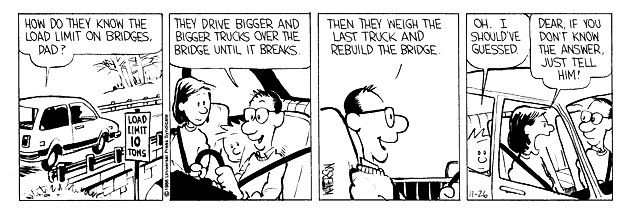
\includegraphics[width = .8\textwidth]{images/CalvinBridgeLoad2.png}
\end{center}

% \noindent Or maybe not quite like that one.

\section*{Thought experiment -- How many dimes?}
Here's a thought experiment for you.  Suppose a middle school class has collected a 
large number of dimes (10-cent coinds) in a sack.  Before bringing the money to the bank, they would like
to estimate how many dimes they have (using tools and methods that 6th graders have at
their disposal).  You've been brought in to consult with them about how they should do this.
\begin{enumerate}
	\item
What method would you suggest?  Why?
\item
What other methods would be possible?  What makes your proposed method better?
\item
For your favorite method and others, identify factors that lead the resulting estimate
to be different from the exact number of dimes in the sack.  
\end{enumerate}


\section*{Some important terms}

\begin{description}
	\item[estimand/measureand]{ The number we want to know.  The ``truth." 
    In our example this is the number
		of dimes in the bag.  Typically this will be a number that describes some process
		or population, and typically it will be impossible to know the value exactly.}

	\item[estimate/measurement]{The value calculated from our data.  This may be 
		as simple as recording a value reported by some device, or it may involve
		recording multiple values, perhaps of multiple variables, maybe at multiple times,
    and making some computations with that data.}  

	\item[error]{The difference between the estimate and the estimand.  Because we don't
		know the estimand exactly, we can't know the error exactly either.  But thinking
		about what the error could be is a big part of understanding the statistical
		properties of an estimation method.  Generally, we want methods where errors 
		tend to be small (so our estimate is ``likely to be close to the estimand")
		and centered around 0 (so we're ``right on average").}
	\item
		[systematic (component of) error]{a component of error that makes our estimate
    biased -- in other words, leads the estimate to be either an over- or under-estimate.
    For example, neglecting the weight of the sack would
		lead us to overestimate the weight of the dimes, and therefore overestimate 
		the number of dimes.  Another way to express this idea is ``a tendency to be off in
		a certain direction."}
	\item
		[random (component of) error]{a component of error that leads to variability
		in estimates (but not a particular tendency toward over- or under-estimation).
    If random errors are larger, there will be more variability 
		in estimates, so we will be less confident that the estimand and estimate are 
		close together -- although some estimates may still be very close to the estimand,
    just by chance.}
\end{description}

One of the big questions in statistics is this:  
\emph{What does our estimate tell us about the estimand?}
We will eventually learn techniques for quantifying (and attempting to reduce)
the effects of error in our measurements. 





\Chapter{Graphical Summaries of Data}



\section{Getting Started With \RStudio}

\begin{figure}
\begin{center}
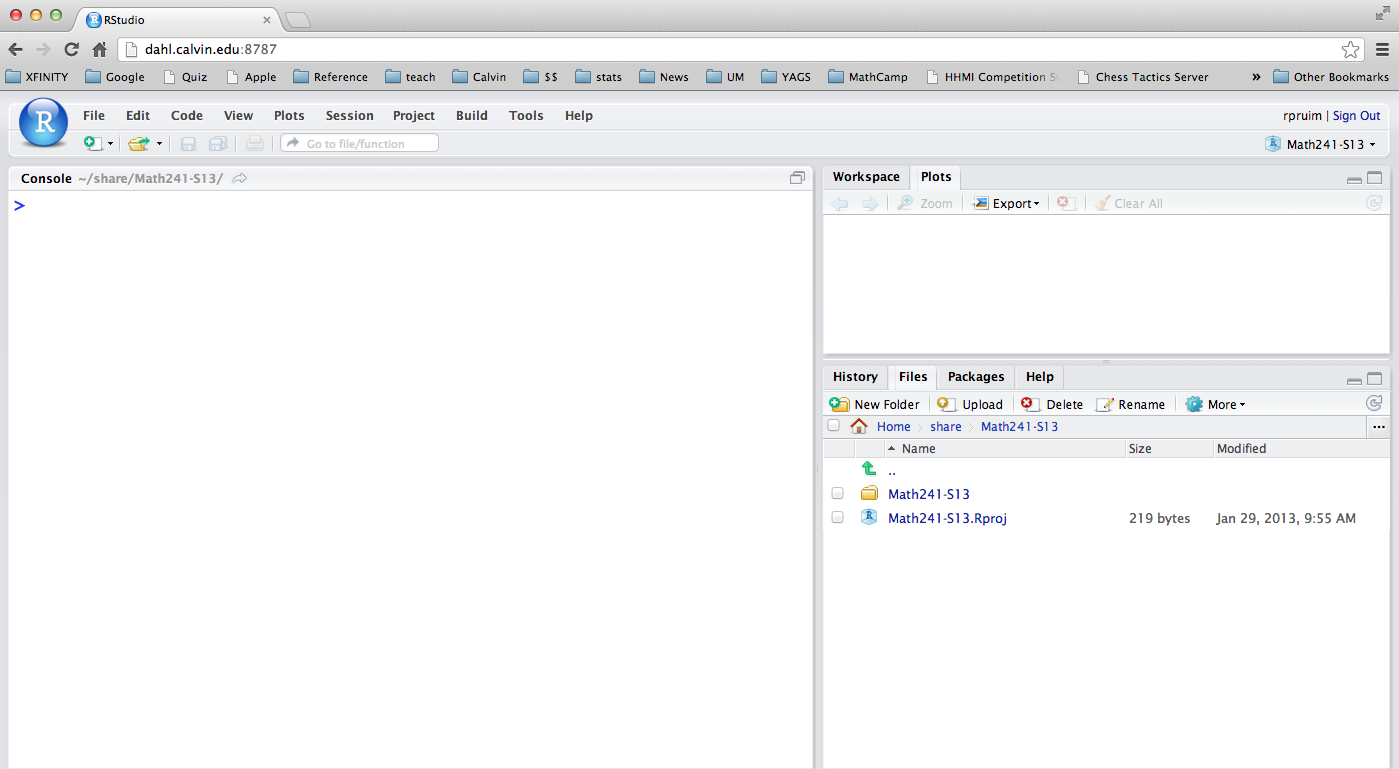
\includegraphics[width = .85\textwidth]{images/RStudio-Welcome.png}
\end{center}
\caption{Welcome to \Rstudio.}
\label{fig:Rstudio-welcome}%
\end{figure}

%You can access the Calvin \RStudio{} server via links from our course
%web site (\url{http://www.calvin.edu/~rpruim/courses/m241/S13/}) or from
%\url{http://dahl.calvin.edu}.
\RStudio{} is an integrated development environment (IDE) for \R,  
a freely available language and environment for statistical computing and graphics.
Both are freely available for Mac, PC, and Linux.  

In addition to running \RStudio{} on your local machine, you have the option
of accessing an \RStudio{} server via a web browser.  (For best results, avoid 
Internet Explorer.)

% \subsection{Logging in and changing your password}
% When you navigate to an \RStudio{} server, you will be prompted to login.  
% % Your login and password are both your Calvin
% % userid.  
% Once you are logged in, you will see something like 
% Figure~\ref{fig:Rstudio-welcome}.
% 
% To change your password:
% \begin{enumerate}
% 	\item From the \tab{Tools} menu, select \tab{Shell...}
% 	\item
% 		Type \code{yppasswd}
% 	\item
% 		You will be prompted for your old password, then your new password twice.
% 	\item
% 		If you give a sufficiently strong new password, then
% 		you will receive notice that your password has been reset.  
% 		If there was a problem, you will see a message about it and can try again.
% 	\item
% 		Once you have reset your password, click on \tab{Close} to close the 
% 		shell and get back to \RStudio.
% \end{enumerate}

\subsection{Using R as a calculator}

Notice that \Rstudio\ divides its world into four panels.  Several of the panels
are further subdivided into multiple tabs.
The console panel is where we type commands that \R\ will execute. 

\R\ can be used as a calculator.  Try typing the following commands in the console panel.
\Rindex{sqrt()}%
\Rindex{log()}%
\Rindex{log10()}%
\begin{knitrout}
\definecolor{shadecolor}{rgb}{0.969, 0.969, 0.969}\color{fgcolor}\begin{kframe}
\begin{alltt}
\hlnum{5} \hlopt{+} \hlnum{3}
\end{alltt}
\begin{verbatim}
## [1] 8
\end{verbatim}
\begin{alltt}
\hlnum{15.3} \hlopt{*} \hlnum{23.4}
\end{alltt}
\begin{verbatim}
## [1] 358
\end{verbatim}
\begin{alltt}
\hlkwd{sqrt}\hlstd{(}\hlnum{16}\hlstd{)}
\end{alltt}
\begin{verbatim}
## [1] 4
\end{verbatim}
\end{kframe}
\end{knitrout}
You can save values to named variables for later reuse
\begin{knitrout}
\definecolor{shadecolor}{rgb}{0.969, 0.969, 0.969}\color{fgcolor}\begin{kframe}
\begin{alltt}
\hlstd{product} \hlkwb{=} \hlnum{15.3} \hlopt{*} \hlnum{23.4}       \hlcom{# save result}
\hlstd{product}                     \hlcom{# show the result}
\end{alltt}
\begin{verbatim}
## [1] 358
\end{verbatim}
\begin{alltt}
\hlstd{product} \hlkwb{<-} \hlnum{15.3} \hlopt{*} \hlnum{23.4}      \hlcom{# <- is assignment operator, same as =}
\hlstd{product}
\end{alltt}
\begin{verbatim}
## [1] 358
\end{verbatim}
\begin{alltt}
\hlnum{15.3} \hlopt{*} \hlnum{23.4} \hlkwb{->} \hlstd{newproduct}   \hlcom{# -> assigns to the right}
\hlstd{newproduct}
\end{alltt}
\begin{verbatim}
## [1] 358
\end{verbatim}
\begin{alltt}
\hlnum{.5} \hlopt{*} \hlstd{product}                \hlcom{# half of the product}
\end{alltt}
\begin{verbatim}
## [1] 179
\end{verbatim}
\begin{alltt}
\hlkwd{log}\hlstd{(product)}                \hlcom{# (natural) log of the product}
\end{alltt}
\begin{verbatim}
## [1] 5.881
\end{verbatim}
\begin{alltt}
\hlkwd{log10}\hlstd{(product)}              \hlcom{# base 10 log of the product}
\end{alltt}
\begin{verbatim}
## [1] 2.554
\end{verbatim}
\begin{alltt}
\hlkwd{log}\hlstd{(product,} \hlkwc{base} \hlstd{=} \hlnum{2}\hlstd{)}        \hlcom{# base 2 log of the product}
\end{alltt}
\begin{verbatim}
## [1] 8.484
\end{verbatim}
\end{kframe}
\end{knitrout}

The semi-colon can be used to place multiple commands on one line.  
One frequent use of this is to save and print a value all in one go:
\begin{knitrout}
\definecolor{shadecolor}{rgb}{0.969, 0.969, 0.969}\color{fgcolor}\begin{kframe}
\begin{alltt}
\hlnum{15.3} \hlopt{*} \hlnum{23.4} \hlkwb{->} \hlstd{product; product}    \hlcom{# save result and show it}
\end{alltt}
\begin{verbatim}
## [1] 358
\end{verbatim}
\end{kframe}
\end{knitrout}

\subsection{Loading packages}

\R\ is divided up into packages.  A few of these are loaded every time you
run \R, but most have to be selected.  This way you only have as much of \R\ as you
need.

In the \tab{Packages} tab, check the boxes next to the following packages to
load them:
\begin{itemize}
	\item \pkg{mosaic}  (a package from Project MOSAIC)
	\item \pkg{DAAG}  (a package that goes with the book \textit{Data Analysis and Graphic})
\end{itemize}
You an also load packages by typing, for example
\begin{knitrout}
\definecolor{shadecolor}{rgb}{0.969, 0.969, 0.969}\color{fgcolor}\begin{kframe}
\begin{alltt}
\hlkwd{library}\hlstd{(DAAG)}       \hlcom{# loads the DAAG package if it is not already loaded}
\end{alltt}
\end{kframe}
\end{knitrout}

\subsection{Four Things to Know About \R}
\begin{enumerate}
\item \R\ is case-sensitive

If you mis-capitalize something in \R, it won't do what you want.

\item 
Functions in \R\ use the following syntax:
\begin{knitrout}
\definecolor{shadecolor}{rgb}{0.969, 0.969, 0.969}\color{fgcolor}\begin{kframe}
\begin{alltt}
\hlkwd{functionname}\hlstd{( argument1, argument2, ... )}
\end{alltt}
\end{kframe}
\end{knitrout}
\vspace{-5mm}
\begin{itemize}
\item The arguments are \underline{always} \emph{surrounded by (round) parentheses} and 
\emph{separated by commas}.

Some functions (like \function{data()}) 
have no required arguments, but you still need the parentheses.

\item
If you type a function name without the parentheses, you will see the \emph{code} for that
function -- which probably isn't what you want at this point.
\end{itemize}
\item
TAB completion and arrows can improve typing speed and accuracy.

If you begin a command and hit the TAB key, \R\ will show you a list of
possible ways to complete the command.  If you hit TAB after the opening
parenthesis of a function, it will show you the list of arguments it expects.
The up and down arrows can be used to retrieve past commands.
\item Hit ESCAPE to break out of a mess.
	
	If you get into some sort of mess typing (usually indicated by extra '$+$' 
	signs along the left edge, indicating that \R\ is waiting for more 
	input -- perhaps because you have some sort of error in what has gone before), 
	you can hit the escape key to get back to a clean prompt.
\end{enumerate}


\section{Data in \R}

\myindex{data frame}%
\myindex{observation unit}%
\myindex{variable}%

\subsection{Data Frames}
Most often, data sets in \R\ are stored in a structure called a 
\term{data frame}.  A data frame is designed to hold ``rectangular data".  
The people or things being measured or observed are called 
\term{observational units} (or subjects or cases when they are people).  
Each observational unit is represented by one row. 
The different pieces of information recorded for each observational unit are stored in
separate columns, called \term{variables}.  

\subsection{Data in Packages}
There are a number of data sets built into \R\
and many more that come in various add on packages.  

You can see a list of data sets in a particular package like this:
\begin{knitrout}
\definecolor{shadecolor}{rgb}{0.969, 0.969, 0.969}\color{fgcolor}\begin{kframe}
\begin{alltt}
\hlkwd{library}\hlstd{(mosaicData)}            \hlcom{# load the package}
\hlkwd{data}\hlstd{(}\hlkwc{package} \hlstd{=} \hlstr{"mosaicData"}\hlstd{)}   \hlcom{# see what data sets are in it}
\end{alltt}
\end{kframe}
\end{knitrout}

You can find a longer list of all data sets available in any loaded package
using 
\begin{knitrout}
\definecolor{shadecolor}{rgb}{0.969, 0.969, 0.969}\color{fgcolor}\begin{kframe}
\begin{alltt}
\hlkwd{data}\hlstd{()}
\end{alltt}
\end{kframe}
\end{knitrout}


\subsection{The HELPrct data set}
The \dataframe{HELPrct} data frame from the \pkg{mosaic} package
contains data from the Health Evaluation and Linkage to Primary Care
randomized clinical trial.  You can find out more about the study and
the data in this data frame by typing
\begin{knitrout}
\definecolor{shadecolor}{rgb}{0.969, 0.969, 0.969}\color{fgcolor}\begin{kframe}
\begin{alltt}
\hlopt{?}\hlstd{HELPrct}
\end{alltt}
\end{kframe}
\end{knitrout}

Among other things, this will tell us something about the subjects (observational units) in
this study:
\begin{quote}
	Eligible subjects were adults, who spoke Spanish or English, reported
	alcohol, heroin or cocaine as their first or second drug of choice, resided
	in proximity to the primary care clinic to which they would be referred or
	were homeless. Patients with established primary care relationships they
	planned to continue, significant dementia, specific plans to leave the
	Boston area that would prevent research participation, failure to provide
	contact information for tracking purposes, or pregnancy were excluded.

Subjects were interviewed at baseline during their detoxification stay and
follow-up interviews were undertaken every 6 months for 2 years.
\end{quote}

It is often handy to look at the first few rows of a data frame.  It will
show you the names of the variables and the kind of data in them:
\begin{knitrout}
\definecolor{shadecolor}{rgb}{0.969, 0.969, 0.969}\color{fgcolor}\begin{kframe}
\begin{alltt}
\hlkwd{head}\hlstd{(HELPrct)}
\end{alltt}
\begin{verbatim}
##   age anysubstatus anysub cesd d1 daysanysub dayslink drugrisk e2b female    sex g1b
## 1  37            1    yes   49  3        177      225        0  NA      0   male yes
## 2  37            1    yes   30 22          2       NA        0  NA      0   male yes
## 3  26            1    yes   39  0          3      365       20  NA      0   male  no
## 4  39            1    yes   15  2        189      343        0   1      1 female  no
## 5  32            1    yes   39 12          2       57        0   1      0   male  no
## 6  47            1    yes    6  1         31      365        0  NA      1 female  no
##   homeless i1 i2 id indtot linkstatus link    mcs   pcs pss_fr racegrp satreat sexrisk
## 1   housed 13 26  1     39          1  yes 25.112 58.41      0   black      no       4
## 2 homeless 56 62  2     43         NA <NA> 26.670 36.04      1   white      no       7
## 3   housed  0  0  3     41          0   no  6.763 74.81     13   black      no       2
## 4   housed  5  5  4     28          0   no 43.968 61.93     11   white     yes       4
## 5 homeless 10 13  5     38          1  yes 21.676 37.35     10   black      no       6
## 6   housed  4  4  6     29          0   no 55.509 46.48      5   black      no       5
##   substance treat avg_drinks max_drinks hospitalizations
## 1   cocaine   yes         13         26                3
## 2   alcohol   yes         56         62               22
## 3    heroin    no          0          0                0
## 4    heroin    no          5          5                2
## 5   cocaine    no         10         13               12
## 6   cocaine   yes          4          4                1
\end{verbatim}
\end{kframe}
\end{knitrout}

When there are a lot of variable, this format is hard to read.  The \function{glimps()} or \function{inspect()}
functions proved some other options.

\begin{knitrout}
\definecolor{shadecolor}{rgb}{0.969, 0.969, 0.969}\color{fgcolor}\begin{kframe}
\begin{alltt}
\hlkwd{glimpse}\hlstd{(HELPrct)}
\end{alltt}
\begin{verbatim}
## Rows: 453
## Columns: 30
## $ age              <int> 37, 37, 26, 39, 32, 47, 49, 28, 50, 39, 34, 58, 58, 60, 36, ...
## $ anysubstatus     <int> 1, 1, 1, 1, 1, 1, NA, 1, 1, 1, NA, 0, 1, 1, 1, 1, 1, 0, 0, 1...
## $ anysub           <fct> yes, yes, yes, yes, yes, yes, NA, yes, yes, yes, NA, no, yes...
## $ cesd             <int> 49, 30, 39, 15, 39, 6, 52, 32, 50, 46, 46, 49, 22, 36, 43, 3...
## $ d1               <int> 3, 22, 0, 2, 12, 1, 14, 1, 14, 4, 0, 3, 5, 10, 2, 6, 1, 2, 0...
## $ daysanysub       <int> 177, 2, 3, 189, 2, 31, NA, 47, 31, 115, NA, 192, 6, 6, 0, 27...
## $ dayslink         <int> 225, NA, 365, 343, 57, 365, 334, 365, 365, 382, 365, 365, 36...
## $ drugrisk         <int> 0, 0, 20, 0, 0, 0, 0, 7, 18, 20, 8, 0, 0, 0, 0, 0, 0, 0, 10,...
## $ e2b              <int> NA, NA, NA, 1, 1, NA, 1, 8, 7, 3, NA, NA, NA, 1, NA, 2, NA, ...
## $ female           <int> 0, 0, 0, 1, 0, 1, 1, 0, 1, 0, 1, 1, 0, 0, 0, 1, 0, 0, 1, 0, ...
## $ sex              <fct> male, male, male, female, male, female, female, male, female...
## $ g1b              <fct> yes, yes, no, no, no, no, yes, yes, no, no, no, no, no, no, ...
## $ homeless         <fct> housed, homeless, housed, housed, homeless, housed, housed, ...
## $ i1               <int> 13, 56, 0, 5, 10, 4, 13, 12, 71, 20, 0, 13, 20, 13, 51, 0, 0...
## $ i2               <int> 26, 62, 0, 5, 13, 4, 20, 24, 129, 27, 0, 13, 31, 20, 51, 0, ...
## $ id               <int> 1, 2, 3, 4, 5, 6, 7, 8, 9, 10, 11, 12, 14, 15, 16, 17, 18, 1...
## $ indtot           <int> 39, 43, 41, 28, 38, 29, 38, 44, 44, 44, 34, 11, 40, 41, 38, ...
## $ linkstatus       <int> 1, NA, 0, 0, 1, 0, 0, 0, 0, 0, 0, 0, 0, 1, 0, 1, 0, 0, 1, 0,...
## $ link             <fct> yes, NA, no, no, yes, no, no, no, no, no, no, no, no, yes, n...
## $ mcs              <dbl> 25.112, 26.670, 6.763, 43.968, 21.676, 55.509, 21.793, 9.161...
## $ pcs              <dbl> 58.41, 36.04, 74.81, 61.93, 37.35, 46.48, 24.52, 65.14, 38.2...
## $ pss_fr           <int> 0, 1, 13, 11, 10, 5, 1, 4, 5, 0, 0, 13, 13, 1, 1, 7, 9, 1, 1...
## $ racegrp          <fct> black, white, black, white, black, black, black, white, whit...
## $ satreat          <fct> no, no, no, yes, no, no, yes, yes, no, yes, no, yes, yes, no...
## $ sexrisk          <int> 4, 7, 2, 4, 6, 5, 8, 6, 8, 0, 2, 0, 1, 4, 8, 3, 4, 4, 3, 7, ...
## $ substance        <fct> cocaine, alcohol, heroin, heroin, cocaine, cocaine, cocaine,...
## $ treat            <fct> yes, yes, no, no, no, yes, no, yes, no, yes, yes, no, no, ye...
## $ avg_drinks       <int> 13, 56, 0, 5, 10, 4, 13, 12, 71, 20, 0, 13, 20, 13, 51, 0, 0...
## $ max_drinks       <int> 26, 62, 0, 5, 13, 4, 20, 24, 129, 27, 0, 13, 31, 20, 51, 0, ...
## $ hospitalizations <int> 3, 22, 0, 2, 12, 1, 14, 1, 14, 4, 0, 3, 5, 10, 2, 6, 1, 2, 0...
\end{verbatim}
\begin{alltt}
\hlkwd{inspect}\hlstd{(HELPrct)}
\end{alltt}
\begin{verbatim}
## 
## categorical variables:  
##        name  class levels   n missing                                  distribution
## 1    anysub factor      2 246     207 yes (77.2%), no (22.8%)                      
## 2       sex factor      2 453       0 male (76.4%), female (23.6%)                 
## 3       g1b factor      2 453       0 no (72%), yes (28%)                          
## 4  homeless factor      2 453       0 housed (53.9%), homeless (46.1%)             
## 5      link factor      2 431      22 no (62.2%), yes (37.8%)                      
## 6   racegrp factor      4 453       0 black (46.6%), white (36.6%) ...             
## 7   satreat factor      2 453       0 no (71.5%), yes (28.5%)                      
## 8 substance factor      3 453       0 alcohol (39.1%), cocaine (33.6%) ...         
## 9     treat factor      2 453       0 no (50.3%), yes (49.7%)                      
## 
## quantitative variables:  
##                   name   class    min     Q1 median     Q3    max     mean       sd   n
## ...1               age integer 19.000  30.00  35.00  40.00  60.00  35.6534   7.7103 453
## ...2      anysubstatus integer  0.000   1.00   1.00   1.00   1.00   0.7724   0.4202 246
## ...3              cesd integer  1.000  25.00  34.00  41.00  60.00  32.8477  12.5145 453
## ...4                d1 integer  0.000   1.00   2.00   3.00 100.00   3.0596   6.1876 453
## ...5        daysanysub integer  0.000   5.00  33.00 164.25 268.00  75.3074  79.2374 244
## ...6          dayslink integer  2.000  74.00 361.00 365.00 456.00 255.6056 151.0227 431
## ...7          drugrisk integer  0.000   0.00   0.00   1.00  21.00   1.8872   4.3365 452
## ...8               e2b integer  1.000   1.00   2.00   3.00  21.00   2.5047   2.5245 214
## ...9            female integer  0.000   0.00   0.00   0.00   1.00   0.2362   0.4252 453
## ...10               i1 integer  0.000   3.00  13.00  26.00 142.00  17.9073  20.0202 453
## ...11               i2 integer  0.000   4.00  18.00  33.00 184.00  24.5475  28.0202 453
## ...12               id integer  1.000 119.00 233.00 348.00 470.00 233.4018 134.7467 453
## ...13           indtot integer  4.000  32.00  38.00  41.00  45.00  35.7285   7.1522 453
## ...14       linkstatus integer  0.000   0.00   0.00   1.00   1.00   0.3782   0.4855 431
## ...15              mcs numeric  6.763  21.68  28.60  40.94  62.18  31.6767  12.8393 453
## ...16              pcs numeric 14.074  40.38  48.88  56.95  74.81  48.0485  10.7846 453
## ...17           pss_fr integer  0.000   3.00   7.00  10.00  14.00   6.7064   3.9950 453
## ...18          sexrisk integer  0.000   3.00   4.00   6.00  14.00   4.6424   2.8002 453
## ...19       avg_drinks integer  0.000   3.00  13.00  26.00 142.00  17.9073  20.0202 453
## ...20       max_drinks integer  0.000   4.00  18.00  33.00 184.00  24.5475  28.0202 453
## ...21 hospitalizations integer  0.000   1.00   2.00   3.00 100.00   3.0596   6.1876 453
##       missing
## ...1        0
## ...2      207
## ...3        0
## ...4        0
## ...5      209
## ...6       22
## ...7        1
## ...8      239
## ...9        0
## ...10       0
## ...11       0
## ...12       0
## ...13       0
## ...14      22
## ...15       0
## ...16       0
## ...17       0
## ...18       0
## ...19       0
## ...20       0
## ...21       0
\end{verbatim}
\end{kframe}
\end{knitrout}

From this we see that there are 453 observational
units in this data set and 30 variables.
That's plenty of variables to get us started with exploration of data.

\subsection{The KidsFeet data set}
Here is another data set in the \pkg{mosaic} package:
\begin{knitrout}
\definecolor{shadecolor}{rgb}{0.969, 0.969, 0.969}\color{fgcolor}\begin{kframe}
\begin{alltt}
\hlkwd{head}\hlstd{(KidsFeet)}
\end{alltt}
\begin{verbatim}
##     name birthmonth birthyear length width sex biggerfoot domhand
## 1  David          5        88   24.4   8.4   B          L       R
## 2   Lars         10        87   25.4   8.8   B          L       L
## 3   Zach         12        87   24.5   9.7   B          R       R
## 4   Josh          1        88   25.2   9.8   B          L       R
## 5   Lang          2        88   25.1   8.9   B          L       R
## 6 Scotty          3        88   25.7   9.7   B          R       R
\end{verbatim}
\end{kframe}
\end{knitrout}

\subsection{The oldfaith data set}
A final example data set comes from the \pkg{alr4} package.  This package is probably not 
loaded (unless you already loaded it).  You can load it from the \tab{Packages} tab or
by typing the command
\begin{knitrout}
\definecolor{shadecolor}{rgb}{0.969, 0.969, 0.969}\color{fgcolor}\begin{kframe}
\begin{alltt}
\hlkwd{library}\hlstd{(alr4)}      \hlcom{# require(alr4) will also work}
\end{alltt}
\end{kframe}
\end{knitrout}
Once you have done that, you will have access to the data set containing information about
Old Faithful eruptions.
\begin{knitrout}
\definecolor{shadecolor}{rgb}{0.969, 0.969, 0.969}\color{fgcolor}\begin{kframe}
\begin{alltt}
\hlkwd{head}\hlstd{(oldfaith)}
\end{alltt}
\begin{verbatim}
##   Duration Interval
## 1      216       79
## 2      108       54
## 3      200       74
## 4      137       62
## 5      272       85
## 6      173       55
\end{verbatim}
\end{kframe}
\end{knitrout}

If you want to know the size of your data set, you can ask it how many rows and columns it has
with
\function{nrow}, \function{ncol}, or \function{dim}:
\begin{knitrout}
\definecolor{shadecolor}{rgb}{0.969, 0.969, 0.969}\color{fgcolor}\begin{kframe}
\begin{alltt}
\hlkwd{nrow}\hlstd{(oldfaith)}
\end{alltt}
\begin{verbatim}
## [1] 270
\end{verbatim}
\begin{alltt}
\hlkwd{ncol}\hlstd{(oldfaith)}
\end{alltt}
\begin{verbatim}
## [1] 2
\end{verbatim}
\begin{alltt}
\hlkwd{dim}\hlstd{(oldfaith)}
\end{alltt}
\begin{verbatim}
## [1] 270   2
\end{verbatim}
\end{kframe}
\end{knitrout}
In this case we have 270 observations of each of two variables.
In a data frame, the observational units are always in the rows and the variables
are always in the columns.  If you create data for use in \R\ (or most other 
statistical packages), you need to make sure your data are also in this shape.


\subsection{Using your own data}

In the Environment tab you will ``Import Dataset".  Click on this import data 
from a CSV file, Excel spreadsheet, or a few other formats.  When you 
do this, the R code will be displayed, so you can see how it is done in 
\R{} code.

If you are using the RStudio server, you will first need to upload your file to the server (unless you can
access the file via URL).  To do this, choose ``Upload" from the Files tab.


\section{Graphical and Numerical Summaries of Data}

\subsection{The Most Important Template}

Using the \pkg{mosiac} and \pkg{ggformula} packages, 
we can compute a wide variety of graphical and numerical summaries 
using the following general template:

\begin{center}
	\Large 
	\texttt{ \fbox{\texttt{ goal \strut{}}} ( \fbox{\texttt{ y\strut{} }} $\sim$ \fbox{\texttt{ x\strut{} }}, data = \fbox{\texttt{ mydata\strut{} }} ) }
\end{center}
We will see this same template used again for linear and non-linear 
modeling as well, so it is is important to master it.\footnote{This is textbook speak for "you should really 
take note of this -- probably memorize it."}

\begin{itemize}
	\item \texttt{goal}: The name of the function generally describes your goal, 
		the thing you want the computer to produce for you.  In the case of plotting,
		it is the name of the plot.  When we do numerical summaries it will be the 
		name of the numerical summary (mean, median, etc.).
	\item \texttt{y}: For plots, this is the variable that goes on the y-axis. 
	\item \texttt{x}: For plots, this is the variable that goes on the x-axis. 
	\item
		\texttt{formula}: Together, \texttt{y ~ x} is called a \term{formula}.
		Very often we can think of \texttt{y ~ x} as ``y depends on x''.
		We will see that sometimes we can omit \texttt{y} ore replace \texttt{x} with \texttt{.} (there must
		always be something on the right-hand side).  We will even see things like 
		\texttt{y ~ x | z}.  But the most important formula to learn is \texttt{y ~ x}.
	\item
		\texttt{mydata:} A data frame must be given in which the variables mentioned in
		the formula can be found.  Variables not found there will be looked for in the 
		enclosing environment.  Sometimes we will take advantage of this to avoid creating
		a temporary data frame just to make a quick plot, but generally it is best to have
		all the information inside a data frame.
\end{itemize}


\section{Scatterplots}

The most common way to look at two quantitative variables is with a 
scatter plot.  The \pkg{ggformula} function for this is \function{gf_point()}, 
and the basic syntax is

\begin{knitrout}
\definecolor{shadecolor}{rgb}{0.969, 0.969, 0.969}\color{fgcolor}\begin{kframe}
\begin{alltt}
\hlkwd{gf_point}\hlstd{( yvar} \hlopt{~} \hlstd{xvar,} \hlkwc{data} \hlstd{= dataName)}
\end{alltt}
\end{kframe}
\end{knitrout}

Let's look at an example. Let's see how bill length is realted to body mass in some penguins.

\begin{knitrout}
\definecolor{shadecolor}{rgb}{0.969, 0.969, 0.969}\color{fgcolor}\begin{kframe}
\begin{alltt}
\hlkwd{library}\hlstd{(palmerpenguins)}
\end{alltt}


{\ttfamily\noindent\bfseries\color{errorcolor}{\#\# Error in library(palmerpenguins): there is no package called 'palmerpenguins'}}\begin{alltt}
\hlkwd{head}\hlstd{(penguins)}
\end{alltt}


{\ttfamily\noindent\bfseries\color{errorcolor}{\#\# Error in h(simpleError(msg, call)): error in evaluating the argument 'x' in selecting a method for function 'head': object 'penguins' not found}}\begin{alltt}
\hlkwd{gf_point}\hlstd{(bill_length_mm} \hlopt{~} \hlstd{body_mass_g,} \hlkwc{data} \hlstd{= penguins)}
\end{alltt}


{\ttfamily\noindent\bfseries\color{errorcolor}{\#\# Error in gf\_ingredients(formula = gformula, data = data, gg\_object = object, : object 'penguins' not found}}\end{kframe}
\end{knitrout}

That's all there is to it.  We can replace \code{bill_length_mm}, \code{body_mass_g}, and 
\code{penguins} with any variables and data set we like to get the scatter plot we want.

\subsection{Adding Color}

Let's add some color. Consider the next two examples.

\begin{knitrout}
\definecolor{shadecolor}{rgb}{0.969, 0.969, 0.969}\color{fgcolor}\begin{kframe}
\begin{alltt}
\hlkwd{gf_point}\hlstd{(bill_length_mm} \hlopt{~} \hlstd{body_mass_g,} \hlkwc{color} \hlstd{=} \hlstr{"navy"}\hlstd{,} \hlkwc{data} \hlstd{= penguins)}
\end{alltt}


{\ttfamily\noindent\bfseries\color{errorcolor}{\#\# Error in gf\_ingredients(formula = gformula, data = data, gg\_object = object, : object 'penguins' not found}}\end{kframe}
\end{knitrout}

\begin{knitrout}
\definecolor{shadecolor}{rgb}{0.969, 0.969, 0.969}\color{fgcolor}\begin{kframe}
\begin{alltt}
\hlkwd{gf_point}\hlstd{(bill_length_mm} \hlopt{~} \hlstd{body_mass_g,} \hlkwc{color} \hlstd{=} \hlopt{~} \hlstd{species,} \hlkwc{data} \hlstd{= penguins)}
\end{alltt}


{\ttfamily\noindent\bfseries\color{errorcolor}{\#\# Error in gf\_ingredients(formula = gformula, data = data, gg\_object = object, : object 'penguins' not found}}\end{kframe}
\end{knitrout}

\begin{itemize}
\item
In the first we are \term{setting} the color of the dots to be navy.
\item
In the second, we are \term{mapping} color based on \code{species}.
Think of \code{color = ~ species} as ``color depends on  species".
\end{itemize}

\subsection{Transparency and dot size}

With so much data in so little space, overplotting (dots on top of each other) can make 
it hard to see what is going on. We can improve this plot by making the dots smaller
and semi-transparent.

\begin{knitrout}
\definecolor{shadecolor}{rgb}{0.969, 0.969, 0.969}\color{fgcolor}\begin{kframe}
\begin{alltt}
\hlkwd{gf_point}\hlstd{(bill_length_mm} \hlopt{~} \hlstd{body_mass_g,} \hlkwc{color} \hlstd{=} \hlopt{~} \hlstd{species,} \hlkwc{data} \hlstd{= penguins,}
         \hlkwc{size} \hlstd{=} \hlnum{0.8}\hlstd{,} \hlkwc{alpha} \hlstd{=} \hlnum{0.5}\hlstd{)}
\end{alltt}


{\ttfamily\noindent\bfseries\color{errorcolor}{\#\# Error in gf\_ingredients(formula = gformula, data = data, gg\_object = object, : object 'penguins' not found}}\end{kframe}
\end{knitrout}

There are many other options we can use to refine our plots.  We'll learn about some of them as we 
go along. You can use \R{}'s built-in help to find out more.  Our you can type

\begin{knitrout}
\definecolor{shadecolor}{rgb}{0.969, 0.969, 0.969}\color{fgcolor}\begin{kframe}
\begin{alltt}
\hlkwd{gf_point}\hlstd{()}
\end{alltt}


{\ttfamily\noindent\itshape\color{messagecolor}{\#\# gf\_point() uses \\\#\#\ \ \ \  * a formula with shape y \textasciitilde{} x. \\\#\#\ \ \ \  * geom:\ \ point \\\#\#\ \ \ \  * key attributes:\ \ alpha, color, size, shape, fill, group, stroke\\\#\# \\\#\# For more information, try ?gf\_point}}\end{kframe}
\end{knitrout}

\subsection{Conditional plots (aka Faceting)}

The formula for a \pkg{ggformula} plot can be extended to create multiple
panels, called facets, based on a ``condition'', often given by another variable. 
The  general syntax for this becomes
\begin{knitrout}
\definecolor{shadecolor}{rgb}{0.969, 0.969, 0.969}\color{fgcolor}\begin{kframe}
\begin{alltt}
\hlkwd{plotname}\hlstd{( y} \hlopt{~} \hlstd{x} \hlopt{|} \hlstd{condition,} \hlkwc{data} \hlstd{= dataName )}
\end{alltt}
\end{kframe}
\end{knitrout}

You can read the formula \code{y ~ x | condition} as saying that we want to know how y depends on x separately
for each condition.
In our penguins example, we might divide up the data according to the islands on which the penguins were spotted.

\begin{knitrout}
\definecolor{shadecolor}{rgb}{0.969, 0.969, 0.969}\color{fgcolor}\begin{kframe}
\begin{alltt}
\hlkwd{gf_point}\hlstd{(bill_length_mm} \hlopt{~} \hlstd{body_mass_g} \hlopt{|} \hlstd{island,} \hlkwc{color} \hlstd{=} \hlopt{~} \hlstd{species,} \hlkwc{data} \hlstd{= penguins,}
         \hlkwc{size} \hlstd{=} \hlnum{0.8}\hlstd{,} \hlkwc{alpha} \hlstd{=} \hlnum{0.5}\hlstd{)}
\end{alltt}


{\ttfamily\noindent\bfseries\color{errorcolor}{\#\# Error in gf\_ingredients(formula = gformula, data = data, gg\_object = object, : object 'penguins' not found}}\end{kframe}
\end{knitrout}

\subsection{Other types of plots}

A scatter plot will be our most common plot for two quantitative variables, but we can use the same
template for any otehr type of plot.  Here are two examples.

\begin{knitrout}
\definecolor{shadecolor}{rgb}{0.969, 0.969, 0.969}\color{fgcolor}\begin{kframe}
\begin{alltt}
\hlkwd{gf_density2d}\hlstd{(bill_length_mm} \hlopt{~} \hlstd{body_mass_g,} \hlkwc{color} \hlstd{=} \hlopt{~} \hlstd{species,} \hlkwc{data} \hlstd{= penguins,} \hlkwc{alpha} \hlstd{=} \hlnum{0.5}\hlstd{)}
\end{alltt}


{\ttfamily\noindent\bfseries\color{errorcolor}{\#\# Error in gf\_ingredients(formula = gformula, data = data, gg\_object = object, : object 'penguins' not found}}\begin{alltt}
\hlkwd{gf_hex}\hlstd{(bill_length_mm} \hlopt{~} \hlstd{body_mass_g,} \hlkwc{data} \hlstd{= penguins,} \hlkwc{binwidth} \hlstd{=} \hlkwd{c}\hlstd{(}\hlnum{250}\hlstd{,} \hlnum{2}\hlstd{))}
\end{alltt}


{\ttfamily\noindent\bfseries\color{errorcolor}{\#\# Error in gf\_ingredients(formula = gformula, data = data, gg\_object = object, : object 'penguins' not found}}\end{kframe}
\end{knitrout}


\section{Graphing the Distribution of One Variable}

A \textbf{distribution} is described by telling what values occur 
and with what frequency.  That is, the distribution answers two 
questions:
\begin{itemize}
	\item What values?  
	\item How often?
\end{itemize}

Statisticians have devised a number of graphs to help us see 
distributions of a variable visually.  
In these graphs, \R{} can compute the y-variable for us.  In this case, we simply
omit the \code{y} part of the formula, so the
general syntax for making a graph or numerical summary
of one variable in a data frame is
\begin{knitrout}
\definecolor{shadecolor}{rgb}{0.969, 0.969, 0.969}\color{fgcolor}\begin{kframe}
\begin{alltt}
\hlkwd{plotname}\hlstd{(} \hlopt{~} \hlstd{variable,} \hlkwc{data} \hlstd{= dataName )}
\end{alltt}
\end{kframe}
\end{knitrout}
In other words, there are three pieces of information we must provide to 
\R\ in order to get the plot we want:
\begin{itemize}
	\item
		The kind of plot. 
		  (\function{gf_histogram()}, \function{gf_bar()}, 
		 \function{gf_density()}, \function{gf_boxplot()}, etc.) 
	\item
		The name of the variable
	\item
		The name of the data frame this variable is a part of.
\end{itemize}

Note: The same syntax works for numerical summaries as well -- thanks to the \pkg{mosaic}
package we can apply the same syntax for 
		\function{mean}, \function{median}, \function{sd},
		\function{var}, \function{max}, \function{min}, etc.
		Later we will use this syntax again to compute linear and 
		nonlinear models.

\subsection{Histograms (and density plots) for quantitative variables}

Histograms (and density plots) are the two most common ways of displaying the distribution 
of a quantitative variable.


Here are a couple examples:

\begin{knitrout}
\definecolor{shadecolor}{rgb}{0.969, 0.969, 0.969}\color{fgcolor}\begin{kframe}
\begin{alltt}
\hlkwd{gf_histogram}\hlstd{(} \hlopt{~} \hlstd{Duration,} \hlkwc{data} \hlstd{= oldfaith)}
\hlkwd{gf_histogram}\hlstd{(} \hlopt{~} \hlstd{age,} \hlkwc{data} \hlstd{= HELPrct)}
\end{alltt}
\end{kframe}

{\centering 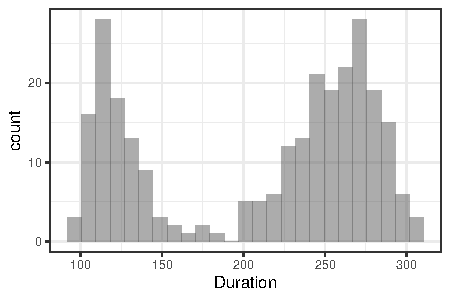
\includegraphics[width=\maxwidth]{figures/fig-histogram-1} 
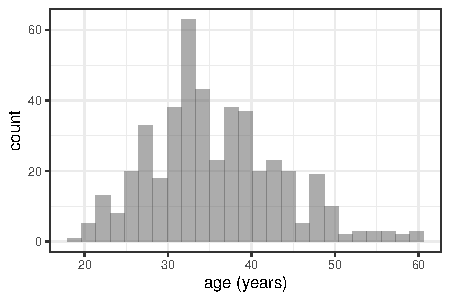
\includegraphics[width=\maxwidth]{figures/fig-histogram-2} 

}



\end{knitrout}

In each of these plots the height of the bar indicates how many observations
fall within the range indicated by the bottom of the bar. So in the histogram below,
the red bar indicates that there are almost 60 eruptions of duration between 100 and 125 seconds
in this data set.

\begin{knitrout}
\definecolor{shadecolor}{rgb}{0.969, 0.969, 0.969}\color{fgcolor}\begin{kframe}
\begin{alltt}
\hlkwd{gf_histogram}\hlstd{(} \hlopt{~} \hlstd{Duration,} \hlkwc{data} \hlstd{= oldfaith,} \hlkwc{binwidth} \hlstd{=} \hlnum{25}\hlstd{,} \hlkwc{boundary} \hlstd{=} \hlnum{100}\hlstd{)} \hlopt
  \hlkwd{gf_histogram}\hlstd{(} \hlopt{~} \hlstd{Duration,} \hlkwc{data} \hlstd{= oldfaith} \hlopt \hlkwd{filter}\hlstd{(Duration} \hlopt{>}\hlnum{100}\hlstd{, Duration} \hlopt{<=} \hlnum{125}\hlstd{),}
                \hlkwc{fill} \hlstd{=} \hlstr{"red"}\hlstd{,} \hlkwc{color} \hlstd{=} \hlstr{"black"}\hlstd{,}
                \hlkwc{binwidth} \hlstd{=} \hlnum{25}\hlstd{,} \hlkwc{boundary} \hlstd{=} \hlnum{100}\hlstd{)}
\end{alltt}
\end{kframe}

{\centering 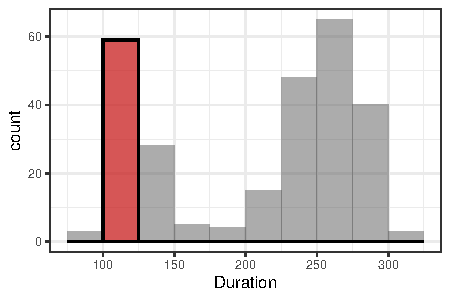
\includegraphics[width=\maxwidth]{figures/fig-histogram-explained-1} 

}



\end{knitrout}

We can control the (approximate) number of bins using the \option{bins}.
The number of bins (and to a lesser extent the positions of the bins)
can make a histogram look quite different.
\begin{knitrout}
\definecolor{shadecolor}{rgb}{0.969, 0.969, 0.969}\color{fgcolor}\begin{kframe}
\begin{alltt}
\hlkwd{gf_histogram}\hlstd{(} \hlopt{~} \hlstd{Duration,} \hlkwc{data} \hlstd{= oldfaith,} \hlkwc{bins} \hlstd{=} \hlnum{8} \hlstd{)}
\hlkwd{gf_histogram}\hlstd{(} \hlopt{~} \hlstd{Duration,} \hlkwc{data} \hlstd{= oldfaith,} \hlkwc{bins} \hlstd{=} \hlnum{15} \hlstd{)}
\hlkwd{gf_histogram}\hlstd{(} \hlopt{~} \hlstd{Duration,} \hlkwc{data} \hlstd{= oldfaith,} \hlkwc{bins} \hlstd{=} \hlnum{30} \hlstd{)}
\end{alltt}
\end{kframe}

{\centering 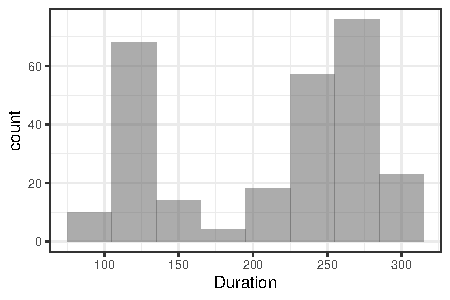
\includegraphics[width=.3\textwidth]{figures/fig-histogram2-1} 
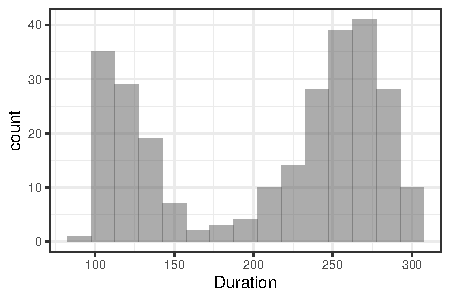
\includegraphics[width=.3\textwidth]{figures/fig-histogram2-2} 
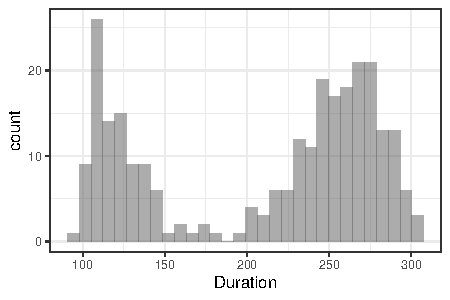
\includegraphics[width=.3\textwidth]{figures/fig-histogram2-3} 

}



\end{knitrout}


We can use \option{binwidth} to set the width of the bins.

\begin{knitrout}
\definecolor{shadecolor}{rgb}{0.969, 0.969, 0.969}\color{fgcolor}\begin{kframe}
\begin{alltt}
\hlkwd{gf_histogram}\hlstd{(} \hlopt{~} \hlstd{Duration,} \hlkwc{data} \hlstd{= oldfaith,} \hlkwc{binwidth} \hlstd{=} \hlnum{60} \hlstd{)}
\hlkwd{gf_histogram}\hlstd{(} \hlopt{~} \hlstd{Duration,} \hlkwc{data} \hlstd{= oldfaith,} \hlkwc{binwidth} \hlstd{=} \hlnum{20} \hlstd{)}
\hlkwd{gf_histogram}\hlstd{(} \hlopt{~} \hlstd{Duration,} \hlkwc{data} \hlstd{= oldfaith,} \hlkwc{binwidth} \hlstd{=} \hlnum{5} \hlstd{)}
\end{alltt}
\end{kframe}

{\centering 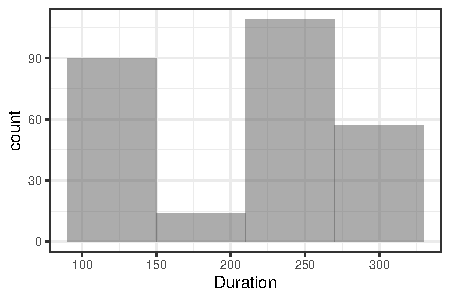
\includegraphics[width=.3\textwidth]{figures/fig-binwidth-1} 
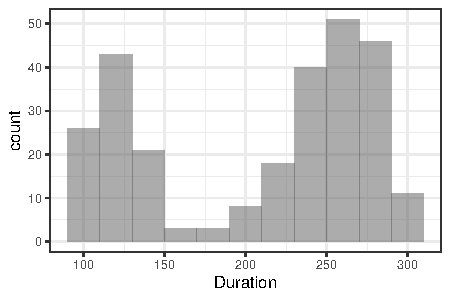
\includegraphics[width=.3\textwidth]{figures/fig-binwidth-2} 
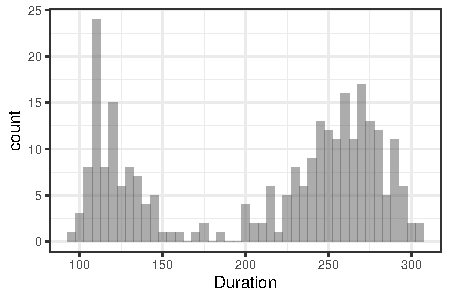
\includegraphics[width=.3\textwidth]{figures/fig-binwidth-3} 

}



\end{knitrout}

\R\ also provides a ``smooth'' version called a density plot and a triangular version
called a frequency polygon:; 

\begin{knitrout}
\definecolor{shadecolor}{rgb}{0.969, 0.969, 0.969}\color{fgcolor}\begin{kframe}
\begin{alltt}
\hlkwd{gf_density}\hlstd{(} \hlopt{~} \hlstd{Duration,} \hlkwc{data} \hlstd{= oldfaith )}
\hlkwd{gf_dens}\hlstd{(} \hlopt{~} \hlstd{Duration,} \hlkwc{data} \hlstd{= oldfaith )}
\hlkwd{gf_freqpoly}\hlstd{(} \hlopt{~} \hlstd{Duration,} \hlkwc{data} \hlstd{= oldfaith )}
\end{alltt}


{\ttfamily\noindent\itshape\color{messagecolor}{\#\# `stat\_bin()` using `bins = 30`. Pick better value with `binwidth`.}}\end{kframe}

{\centering 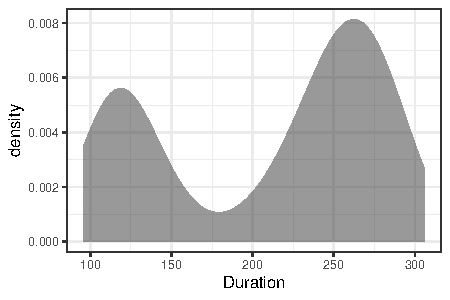
\includegraphics[width=.3\textwidth]{figures/fig-density-1} 
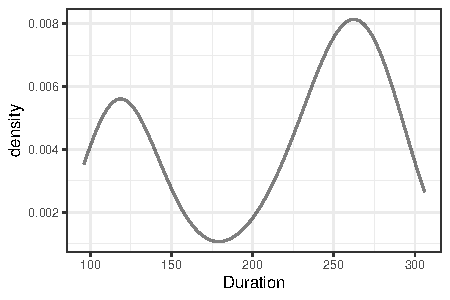
\includegraphics[width=.3\textwidth]{figures/fig-density-2} 
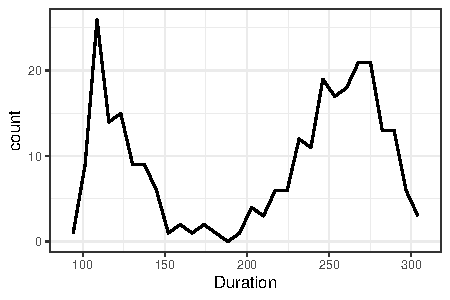
\includegraphics[width=.3\textwidth]{figures/fig-density-3} 

}



\end{knitrout}


\subsection{Describing the shape of a distribution}

If we make a histogram of our data, we can describe the overall shape of the distribution.
Keep in mind that the shape of a particular histogram may depend on the choice of bins.
Choosing too many or too few bins can hide the true shape of the distribution.  (When in doubt, make
more than one histogram.)

Here are some words we use to describe shapes of distributions.
\begin{description}
\item[symmetric] The left and right sides are mirror images of each other.
\item[skewed] The distribution stretches out farther in one direction than in the other.  
(We say the distribution is skewed toward the long tail.)
\item[uniform] The heights of all the bars are (roughly) the same.  
(So the data are equally likely to be anywhere within some range.)
\item[unimodal] There is one major ``bump'' where there is a lot of data.
\item[bimodal] There are two ``bumps''.
\item[outlier] An observation that does not fit the overall pattern of the rest of 
the data.
\end{description}

We'll learn about another graph used for quantitative variables (boxplots)
soon.

\subsection{Bar graphs for categorical variables}

Bar graphs are a way of displaying the distribution of a categorical variable.

\begin{knitrout}
\definecolor{shadecolor}{rgb}{0.969, 0.969, 0.969}\color{fgcolor}\begin{kframe}
\begin{alltt}
\hlkwd{gf_bar}\hlstd{(} \hlopt{~} \hlstd{species,} \hlkwc{data} \hlstd{= penguins)}   \hlcom{# vertical bars}
\end{alltt}


{\ttfamily\noindent\bfseries\color{errorcolor}{\#\# Error in gf\_ingredients(formula = gformula, data = data, gg\_object = object, : object 'penguins' not found}}\begin{alltt}
\hlkwd{gf_bar}\hlstd{(species} \hlopt{~} \hlstd{.,} \hlkwc{data} \hlstd{= penguins)}  \hlcom{# horizontal bars}
\end{alltt}


{\ttfamily\noindent\bfseries\color{errorcolor}{\#\# Error in gf\_ingredients(formula = gformula, data = data, gg\_object = object, : object 'penguins' not found}}\end{kframe}
\end{knitrout}

Statisticians rarely use pie charts because they are harder to read except in a few special cases (like comparing
a proportion to 50\%).

\subsection{Overlaying and faceting data}

Overlaying and faceting work the same for these one variables plots as they did for the scatterplots above.

\begin{knitrout}
\definecolor{shadecolor}{rgb}{0.969, 0.969, 0.969}\color{fgcolor}\begin{kframe}
\begin{alltt}
\hlkwd{gf_bar}\hlstd{(} \hlopt{~} \hlstd{species} \hlopt{|} \hlstd{island,} \hlkwc{data} \hlstd{= penguins)}
\end{alltt}


{\ttfamily\noindent\bfseries\color{errorcolor}{\#\# Error in gf\_ingredients(formula = gformula, data = data, gg\_object = object, : object 'penguins' not found}}\begin{alltt}
\hlkwd{gf_histogram}\hlstd{(} \hlopt{~} \hlstd{body_mass_g} \hlopt{|} \hlstd{species,} \hlkwc{data} \hlstd{= penguins)}
\end{alltt}


{\ttfamily\noindent\bfseries\color{errorcolor}{\#\# Error in gf\_ingredients(formula = gformula, data = data, gg\_object = object, : object 'penguins' not found}}\begin{alltt}
\hlkwd{gf_dens}\hlstd{(} \hlopt{~} \hlstd{body_mass_g,} \hlkwc{color} \hlstd{=} \hlopt{~} \hlstd{species,} \hlkwc{data} \hlstd{= penguins)}
\end{alltt}


{\ttfamily\noindent\bfseries\color{errorcolor}{\#\# Error in gf\_ingredients(formula = gformula, data = data, gg\_object = object, : object 'penguins' not found}}\end{kframe}
\end{knitrout}

For example, we might like to see how the ages of men and women compare 
in the HELP study, or whether the distribution of weights of male mosquitoes 
is different from the distribution for females.

\begin{knitrout}
\definecolor{shadecolor}{rgb}{0.969, 0.969, 0.969}\color{fgcolor}\begin{kframe}
\begin{alltt}
\hlkwd{gf_histogram}\hlstd{(} \hlopt{~} \hlstd{age} \hlopt{|} \hlstd{sex,} \hlkwc{data} \hlstd{= HELPrct,} \hlkwc{binwidth} \hlstd{=} \hlnum{5}\hlstd{)}
\hlkwd{gf_dens}\hlstd{(} \hlopt{~} \hlstd{length} \hlopt{|} \hlstd{sex,} \hlkwc{data} \hlstd{= KidsFeet )}
\end{alltt}
\end{kframe}

{\centering 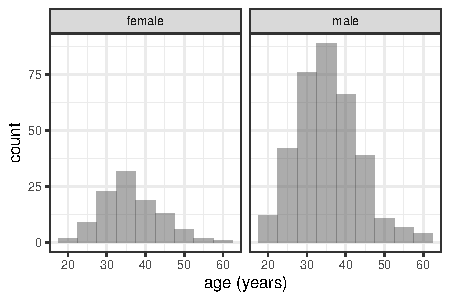
\includegraphics[width=\maxwidth]{figures/fig-compare-ages-1} 
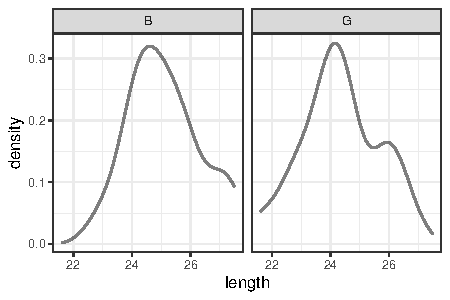
\includegraphics[width=\maxwidth]{figures/fig-compare-ages-2} 

}



\end{knitrout}


We can do the same thing for bar graphs.

\begin{knitrout}
\definecolor{shadecolor}{rgb}{0.969, 0.969, 0.969}\color{fgcolor}\begin{kframe}
\begin{alltt}
\hlkwd{gf_bar}\hlstd{(} \hlopt{~} \hlstd{substance} \hlopt{|} \hlstd{sex,} \hlkwc{data} \hlstd{= HELPrct)}
\end{alltt}
\end{kframe}

{\centering 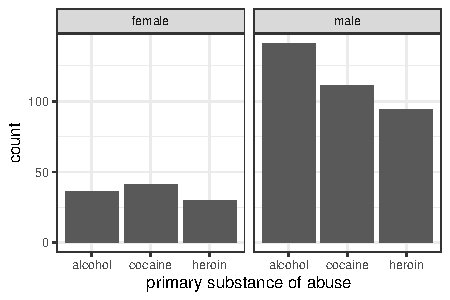
\includegraphics[width=\maxwidth]{figures/fig-substance-by-sex-1} 

}



\end{knitrout}

\subsection{Grouping and bar charts}

When dividing bar charts into multiple colors, we can present the segmented bars "stacked" (the default)
or "dodged":

\begin{knitrout}
\definecolor{shadecolor}{rgb}{0.969, 0.969, 0.969}\color{fgcolor}\begin{kframe}
\begin{alltt}
\hlkwd{gf_bar}\hlstd{(}\hlopt{~}\hlstd{substance,} \hlkwc{fill} \hlstd{=} \hlopt{~}\hlstd{sex,} \hlkwc{data} \hlstd{= HELPrct)}
\hlkwd{gf_bar}\hlstd{(}\hlopt{~}\hlstd{substance,} \hlkwc{fill} \hlstd{=} \hlopt{~}\hlstd{sex,} \hlkwc{data} \hlstd{= HELPrct,} \hlkwc{position} \hlstd{=} \hlstr{"dodge"}\hlstd{)}
\end{alltt}
\end{kframe}

{\centering 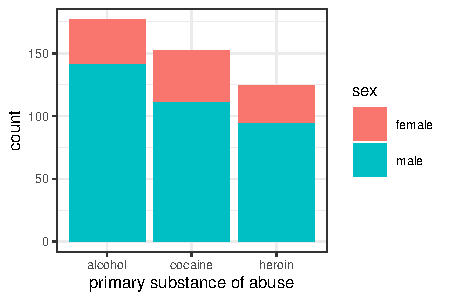
\includegraphics[width=\maxwidth]{figures/fig-groups-1} 
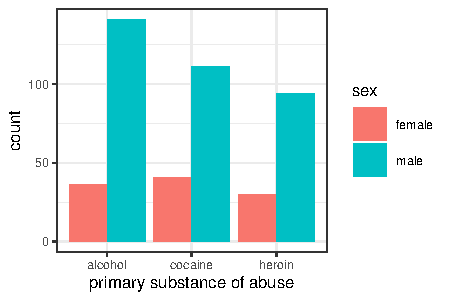
\includegraphics[width=\maxwidth]{figures/fig-groups-2} 

}



\end{knitrout}

\subsection{Proportions and bar charts}

Sometimes it is better to display bars with proportions rather than counts. But then we must decide
what to use for the denominator.
In the first example below, the total of all teh bars adds to 1. In the second plot, the total
adds to one for each x variable, which makes it easier to see how the proportions of male and female
.

\begin{knitrout}
\definecolor{shadecolor}{rgb}{0.969, 0.969, 0.969}\color{fgcolor}\begin{kframe}
\begin{alltt}
\hlkwd{gf_props}\hlstd{(}\hlopt{~}\hlstd{substance,} \hlkwc{fill} \hlstd{=} \hlopt{~}\hlstd{sex,} \hlkwc{data} \hlstd{= HELPrct)}
\hlkwd{gf_props}\hlstd{(}\hlopt{~}\hlstd{substance,} \hlkwc{fill} \hlstd{=} \hlopt{~}\hlstd{sex,} \hlkwc{data} \hlstd{= HELPrct,} \hlkwc{denom} \hlstd{=} \hlopt{~} \hlstd{x)}
\end{alltt}
\end{kframe}

{\centering 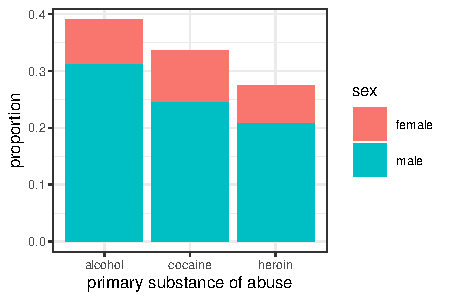
\includegraphics[width=\maxwidth]{figures/fig-gf-props-1} 
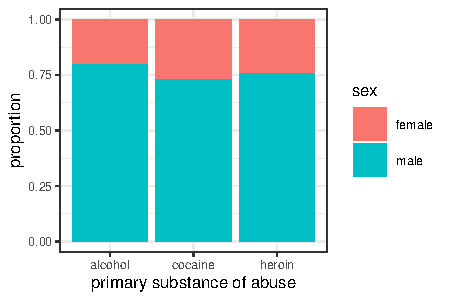
\includegraphics[width=\maxwidth]{figures/fig-gf-props-2} 

}



\end{knitrout}

\section{Labeling plots}

Often the defaults labels are not ideal for publication purposes. You can add titles and captions
and change the labeling of variables using \function{gf_labs()}.

\begin{knitrout}
\definecolor{shadecolor}{rgb}{0.969, 0.969, 0.969}\color{fgcolor}\begin{kframe}
\begin{alltt}
\hlkwd{gf_point}\hlstd{(bill_length_mm} \hlopt{~} \hlstd{body_mass_g} \hlopt{|} \hlstd{island,} \hlkwc{color} \hlstd{=} \hlopt{~} \hlstd{species,} \hlkwc{data} \hlstd{= penguins,}
         \hlkwc{size} \hlstd{=} \hlnum{0.8}\hlstd{,} \hlkwc{alpha} \hlstd{=} \hlnum{0.5}\hlstd{)} \hlopt
  \hlkwd{gf_labs}\hlstd{(}\hlkwc{x} \hlstd{=} \hlstr{"body mass (g)"}\hlstd{,} \hlkwc{y} \hlstd{=} \hlstr{"bill length (mm)"}\hlstd{,}
          \hlkwc{title} \hlstd{=} \hlstr{"Some penguin measurments"}\hlstd{,} \hlkwc{caption} \hlstd{=} \hlstr{"Data Source: palmerpenguins"}\hlstd{)}
\end{alltt}


{\ttfamily\noindent\bfseries\color{errorcolor}{\#\# Error in gf\_ingredients(formula = gformula, data = data, gg\_object = object, : object 'penguins' not found}}\end{kframe}
\end{knitrout}

Notice the \verb!%>%! in the example above.  This important and connects the labeling
below to the plot above.

\section{Exporting Plots}

You can save plots to files or copy them to the clipboard using the 
\tab{Export} menu in the \tab{Plots} tab.  It is quite simple to copy the 
plots to the clipboard and then paste them into a Word document, for example.
You can even adjust the height and width of the plot first to get it the 
shape you want.  \emph{But there are much better ways to produce documents 
with \R{} graphics in them!}  See the next section.

\section{Reproducible Research}

Copy-and-paste is a bad workflow for lots of reasons, including:
\begin{itemize}
	\item It is tedious, unless there is very little to copy and paste.
	\item It is error-prone -- it's easy to copy to little or too much, or to grab the wrong thing,
		or to copy when you want to cut or cut when you want to copy.
	\item
		If something changes, you have to start all over.
	\item
		You have no record of what you did (unless you are an unusual person who
		takes detailed notes about all the copying and pasting).
\end{itemize}
So while copy-and-paste seems easy and convenient, it is not \emph{reproducible}.
Reproducibility is important when projects are large, when it is important to have record of 
exactly what was done, or when the same analysis is applied to multiple data sets (or a data set
that is growing over time).

\RStudio\ makes it easy to use techniques of reproducible research to create
documents that include text, \R\ commands, \R\ output, and \R\ graphics.  

\subsection{R Markdown}
The simplest version of this uses a format called R Markdown.  Markdown is a simple
mark up language that allows for a few basic improvements on plain text
(section headers, bulleted lists, numbered lists, bold, italics, etc.)  R
Markdown adds the ability to mix in the \R\ stuff.  
The end product is an HTML file, so it is especially good for producing web 
documents.\footnote{You can actually mix in arbirary HTML and even css, so if you
are good at HTML, you can have quite a bit of control over how things look.  Here will
will focus on the basics.}

\subsubsection{Creating a new document}
To create a new R Markdown document, go to ``File", ``New File", then ``R Markdown":
\begin{center}
	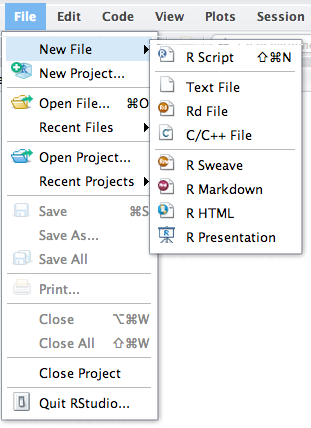
\includegraphics[width = 3in]{images/NewRMarkdown.png}
\end{center}

From there, choose either ``document" or ``from template".  The \pkg{mosaic} plain 
template is a good starting point.

\begin{center}
	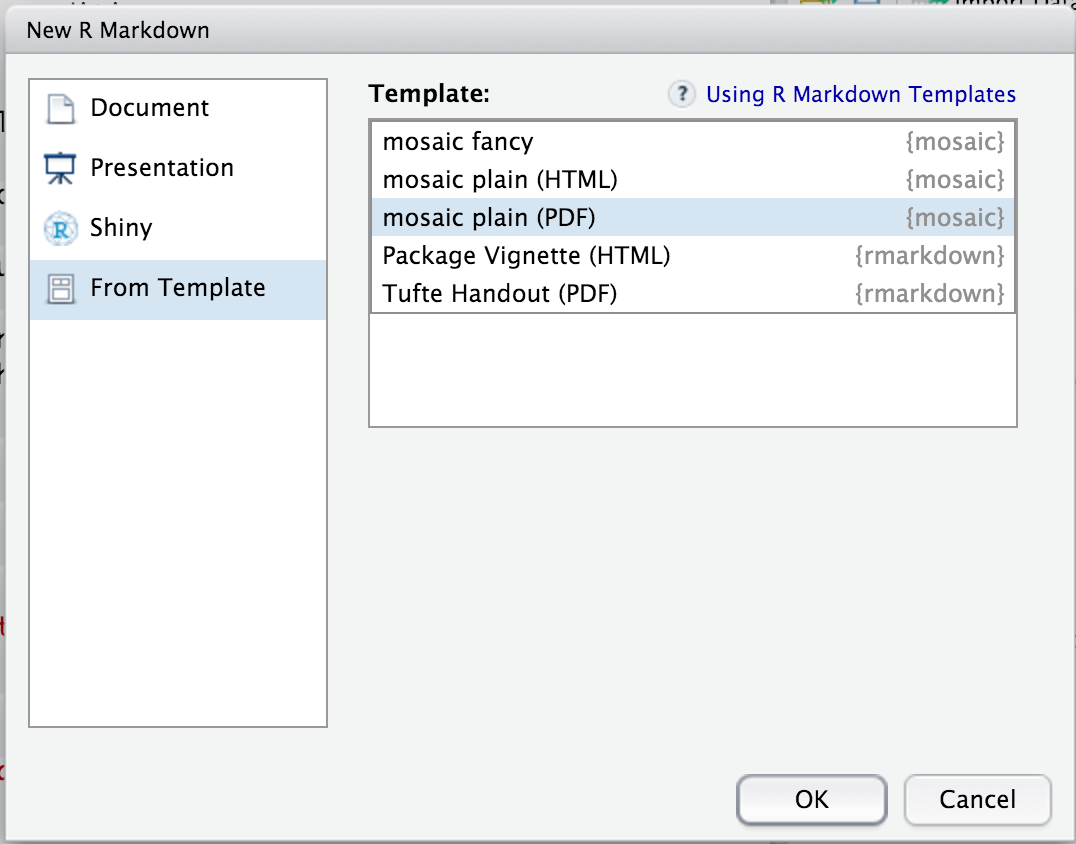
\includegraphics[width = 3in]{images/FromTemplate.png}
\end{center}


When you do this, a file editing pane will open with a template inserted.  If
you click on ``Knit HTML", \RStudio\ will turn this into an HTML file and
display it for you.  Give it a try.  You will be asked to name your file if you
haven't already done so.  If you are using the \RStudio\ server in a browser,
then your file will live on the server (``in the cloud'') rather than on your
computer.

If you look at the template file you will see that the file has two kinds of
sections.  Some of this file is just normal text (with some extra symbols to
make things bold, add in headings, etc.)  You can get a list of all of these
mark up options by selecting the ``Markdown Quick Reference" in the help
menu.

\begin{center}
	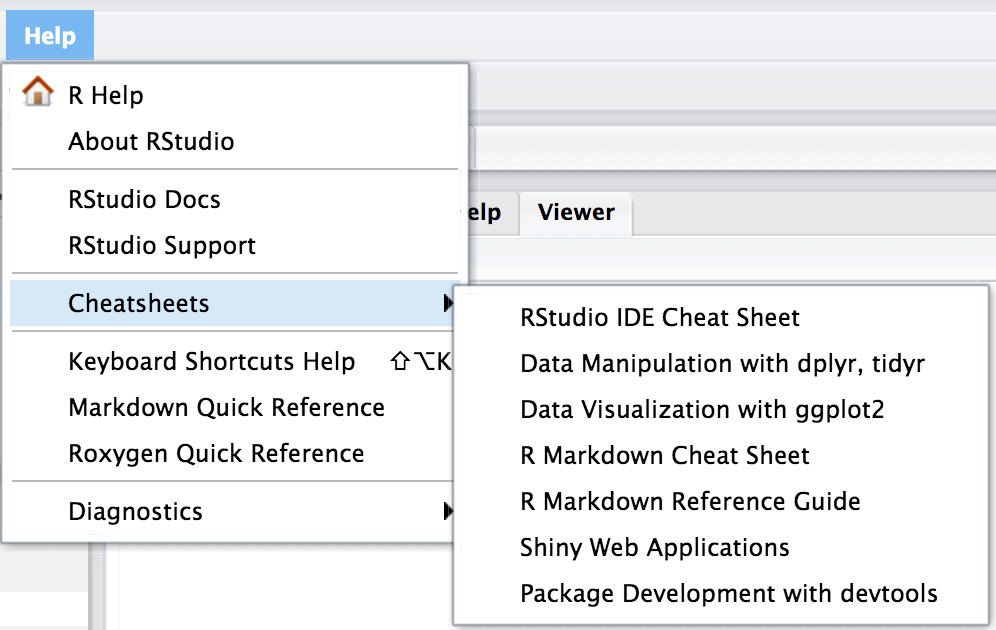
\includegraphics[width = 3.5in]{images/MarkdownQuickReference.png}
\end{center}

The second type of section is an \R\ code chunk.  These are colored differently to make them
easier to see.  You can insert a new code chunk by selecting by selecting
the appropriate chunk type (R in our case) from the menu below.
\begin{center}
	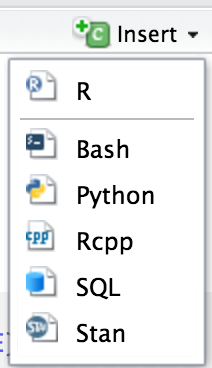
\includegraphics[width = 1.2in]{images/InsertChunk.png}
\end{center}

\noindent
You can also type 
\begin{knitrout}
\definecolor{shadecolor}{rgb}{0.969, 0.969, 0.969}\color{fgcolor}\begin{kframe}
\begin{alltt}
```\{r\}
```
\end{alltt}
\end{kframe}
\end{knitrout}
to begin and end the code chunk if you would rather type.
You can put any \R\ code in these code chunks and the results (text output or graphics) as well
as the \R\ code will be displayed in your HTML file.

%There are options to do things like (a) run \R\ code without displayng it, (b) run \R\ code without
%displaying the output, (c) controling size of plots, etc., etc.  
%But for starting out, this is really all you need to know.

\subsection*{R Markdown files must be self-contained}
R Markdown files do not have access to things you have done in your console.  (This is good, else 
your document would change based on things not in the file.)  This means that you must explicitly
load any data packages that you use \emph{in the R Markdown file}. In this class,
this means that most of your R Markdown files will have a chunk near the beginning that 
includes

\begin{knitrout}
\definecolor{shadecolor}{rgb}{0.969, 0.969, 0.969}\color{fgcolor}\begin{kframe}
\begin{alltt}
\hlkwd{library}\hlstd{(mosaic)}
\end{alltt}
\end{kframe}
\end{knitrout}

\noindent
If you use one of the RMarkdown templates provided, 
this (and some otehr things) will be included in the template and save you some time.

\iffalse
\subsubsection{Creating an R Markdown document}
To create an R Markdown document, choose ``File", then ``New File", then ``R Markdown".  The file
will open with a template already loaded.   Take a quick look and you will see that most 
of this is easy to read.  You can see some text with a few extra symbols thrown in here and 
there and some chunks of \R\ code.
Now click on the "knit HTML" button and this document will be converted to HTML.

To create your own content, simply delete out the things you don't want or need
and replace them with your own content.  If you forget the markup, there is a help button
that will lead you to a quick reference guide.  To add a chunk of \R\ code, click on 
``Chunk" and then ``Insert Chunk" and put your \R\ code inside the chunk.

In addition to knitting the document to HTML, you can do a number of other things that will
make your work more efficient.  In the ``Chunk" menu, you can choose to run a single chunk 
or all the chunks.  This will execute your commands in the console so you can make sure 
your \R\ code is working one chunk at a time.  There is also a ``run" button that allows you
to run just one line from within a chunk.

\subsubsection{R Markdown files do not have access to the console environment}
One thing you need to remember about R Markdown documents is that the file must be self-contained.
This ensures that the document is portable.  It also means that the docuemnt does not have 
access to the things in your console environment.  All data must be loaded in the file.  
Similarly, all packages you use must also be loaded in the file.  If you start getting messages 
about objects not being found, one possible cause is that you have forgotten to get some 
data or some package loaded inside your file.  (Typos are another cause for these messages -- 
check your spelling and capitalization.)
\fi

\subsection{Chunk options}
R Markdown provides a number of chunk options that control how \R\ code is processed.  
You can use them to do things like:
\begin{itemize}
	\item
		run the code without displaying it (good for polished reports -- your client doesn't want to see the code)
	\item
		show the code without running it -- mainly useful for demonstration purposes
	\item
		control the size and alignment of graphics
\end{itemize}
You can set default values for the chunk options and you can also override them in individual
chunks.  See the R Markdown help for more information about chunk options.

The default plots are often bigger than required.  The following chunk options are a place to 
start.  They can be adjusted as necessary.
\begin{knitrout}
\definecolor{shadecolor}{rgb}{0.969, 0.969, 0.969}\color{fgcolor}\begin{kframe}
\begin{alltt}
\hlkwd{library}\hlstd{(knitr)}
\hlstd{opts_chunk}\hlopt{$}\hlkwd{set}\hlstd{(}\hlkwc{fig.width} \hlstd{=} \hlnum{5}\hlstd{,} \hlkwc{fig.height} \hlstd{=} \hlnum{2}\hlstd{,} \hlkwc{fig.align} \hlstd{=} \hlstr{"center"}\hlstd{,} \hlkwc{fig.show} \hlstd{=} \hlstr{"hold"}\hlstd{)}
\end{alltt}
\end{kframe}
\end{knitrout}

Some of these document settings can also be set in the YAML header 
(the top few lines of the RMarkdown file).

\subsection{knitr/latex}
There is another system that produces PDFs by combining \LaTeX\ and \R.  This is the system
used to create this document and it gives much more control over paper-like formatting.  The
quality is good enough for profession publishing.  If you already knwow \LaTeX, it is very
easy to learn.  If you don't know \LaTeX, then you need to learn the basics of \LaTeX\ to get
going, but it isn't very difficult.

\R\ code and output can be copied and pasted as well.  It's best to use a 
fixed width font (like Courier) for \R\ code so that things align properly.

Note:  \RStudio\ provide some nice utilities for creating documents that include
text, code, graphics, and statistical analyses all in one document.  That's how this 
document was produced.  The simpler of these is called RMarkdown.  The resulting file
will be an HTML file with embedded plots.  You can gain more control over the output
by using \pkg{knitr} which provides a way to combine \LaTeX\ and \R in a single
document.  The resulting document in this case is a high quality PDF

\iffalse
\section{A Few Bells and Whistles}
There are lots of arguments that control how these plots look.  Here are just a
few examples, some of which we have already seen.

% \subsection{auto.key}
% \option{auto.key = TRUE} turns on a simple legend for the grouping variable.  
% (There are ways to have more control, if you need it.)
% <<iris-xyplot-key,cache = TRUE,fig.width = 2.6,fig.height = 2.4>>=
% xyplot(Sepal.Length ~ Sepal.Width, groups = Species, data = iris, 
% 	auto.key = TRUE)   
% @

\subsection{alpha, size}
Sometimes it is nice to have elements of a plot be partly transparent.  When
such elements overlap, they get darker, showing us where data are ``piling up."
Setting the \argument{alpha} argument to a value between 0 and 1 controls the
degree of transparency: 1 is completely opaque, 0 is invisible.  The
\argument{size} argument controls the size of lines and points.

Here is another example using data on 150 iris plants of three species.
\begin{knitrout}
\definecolor{shadecolor}{rgb}{0.969, 0.969, 0.969}\color{fgcolor}\begin{kframe}
\begin{alltt}
\hlkwd{gf_point}\hlstd{(Sepal.Length} \hlopt{~} \hlstd{Sepal.Width,} \hlkwc{color} \hlstd{=} \hlopt{~} \hlstd{Species,} \hlkwc{data} \hlstd{= iris,}
        \hlkwc{alpha} \hlstd{=} \hlnum{.5}\hlstd{,}
        \hlkwc{size} \hlstd{=} \hlnum{1.3}\hlstd{)}
\end{alltt}
\end{kframe}

{\centering 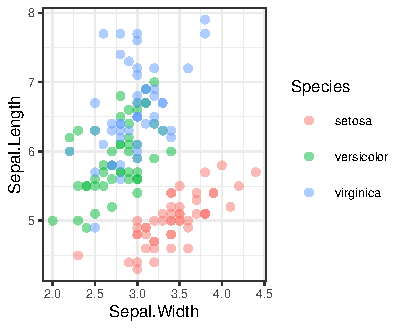
\includegraphics[width=\maxwidth]{figures/fig-iris-xyplot-alpha-1} 

}



\end{knitrout}

\subsection*{main, sub, xlab, ylab}

You can add a title or subtitle, or change the default labels of the axes.
\begin{knitrout}
\definecolor{shadecolor}{rgb}{0.969, 0.969, 0.969}\color{fgcolor}\begin{kframe}
\begin{alltt}
\hlkwd{gf_point}\hlstd{(Sepal.Length} \hlopt{~} \hlstd{Sepal.Width,} \hlkwc{color} \hlstd{=} \hlopt{~}\hlstd{Species,} \hlkwc{data} \hlstd{= iris,}
        \hlkwc{main} \hlstd{=} \hlstr{"Some Iris Data"}\hlstd{,}
        \hlkwc{sub} \hlstd{=} \hlstr{"(R. A. Fisher analysized this data in 1936)"}\hlstd{,}
        \hlkwc{xlab} \hlstd{=} \hlstr{"sepal width (cm)"}\hlstd{,}
        \hlkwc{ylab} \hlstd{=} \hlstr{"sepal length (cm)"}\hlstd{,}
        \hlkwc{alpha} \hlstd{=} \hlnum{.5}
\hlstd{)}
\end{alltt}
\end{kframe}

{\centering 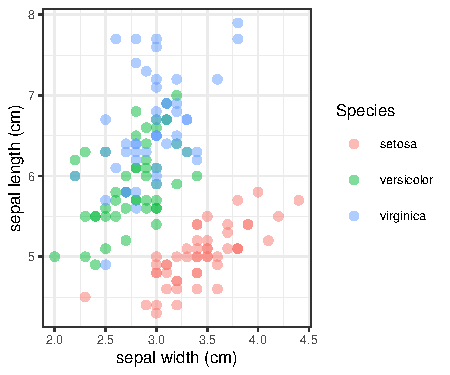
\includegraphics[width=\maxwidth]{figures/fig-iris-xyplot-text-1} 

}



\end{knitrout}


\subsubsection*{linetype, shape}
These can be used to change the line type, line width, plot character, and
color.  To specify multiples (one for each group), use the \function{c()} function 
(see below).

\begin{knitrout}
\definecolor{shadecolor}{rgb}{0.969, 0.969, 0.969}\color{fgcolor}\begin{kframe}
\begin{alltt}
\hlkwd{gf_dens}\hlstd{(} \hlopt{~}\hlstd{age,} \hlkwc{data} \hlstd{= HELPrct,} \hlkwc{color} \hlstd{=} \hlopt{~} \hlstd{sex,} \hlkwc{linetype} \hlstd{=} \hlopt{~} \hlstd{sex)}
\hlkwd{gf_dens}\hlstd{(} \hlopt{~}\hlstd{age,} \hlkwc{data} \hlstd{= HELPrct,} \hlkwc{color} \hlstd{=} \hlopt{~} \hlstd{sex,} \hlkwc{linetype} \hlstd{=} \hlstr{"dotted"}\hlstd{)}
\hlkwd{gf_histogram}\hlstd{(} \hlopt{~} \hlstd{age,} \hlkwc{data} \hlstd{= HELPrct,} \hlkwc{fill} \hlstd{=} \hlstr{'steelblue'}\hlstd{)}
\end{alltt}
\end{kframe}

{\centering 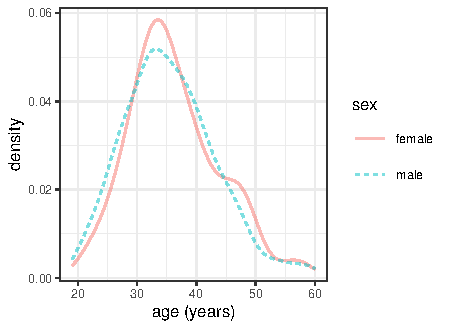
\includegraphics[width=\maxwidth]{figures/fig-pch-lwd-lty-1} 
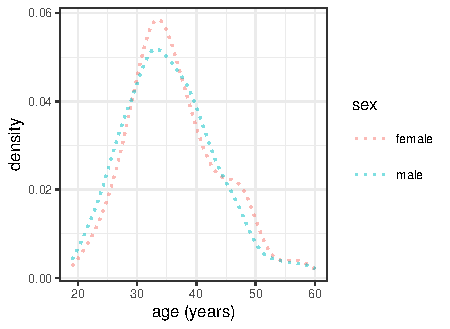
\includegraphics[width=\maxwidth]{figures/fig-pch-lwd-lty-2} 
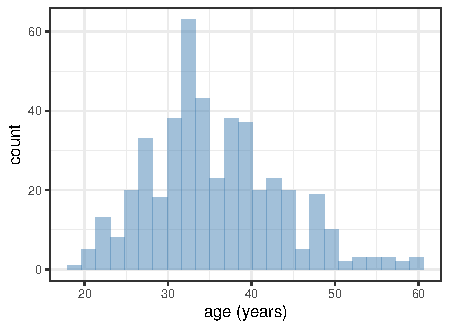
\includegraphics[width=\maxwidth]{figures/fig-pch-lwd-lty-3} 

}



\end{knitrout}

You can see a list of the hundreds of available color names using
\Rindex{colors()}%
\begin{knitrout}
\definecolor{shadecolor}{rgb}{0.969, 0.969, 0.969}\color{fgcolor}\begin{kframe}
\begin{alltt}
\hlkwd{colors}\hlstd{()}
\end{alltt}
\end{kframe}
\end{knitrout}

\subsection{trellis.par.set()}
Default settings for graphics properties can be set as follows:

\begin{knitrout}
\definecolor{shadecolor}{rgb}{0.969, 0.969, 0.969}\color{fgcolor}\begin{kframe}
\begin{alltt}
\hlkwd{theme_set}\hlstd{(}\hlkwd{theme_classic}\hlstd{(}\hlkwc{base_size} \hlstd{=} \hlnum{6}\hlstd{))}    \hlcom{# base size for text is 6 point; classic theme.}
\hlkwd{gf_dens}\hlstd{(} \hlopt{~}\hlstd{age,} \hlkwc{data} \hlstd{= HELPrct,} \hlkwc{color} \hlstd{=} \hlopt{~} \hlstd{sex,} \hlkwc{linetype} \hlstd{=} \hlstr{"dashed"}\hlstd{)}
\hlkwd{theme_set}\hlstd{(}\hlkwd{theme_bw}\hlstd{(}\hlkwc{base_size} \hlstd{=} \hlnum{8}\hlstd{))}
\hlkwd{gf_dens}\hlstd{(} \hlopt{~}\hlstd{age,} \hlkwc{data} \hlstd{= HELPrct,} \hlkwc{color} \hlstd{=} \hlopt{~} \hlstd{sex,} \hlkwc{linetype} \hlstd{=} \hlstr{"dashed"}\hlstd{)}
\end{alltt}
\end{kframe}

{\centering 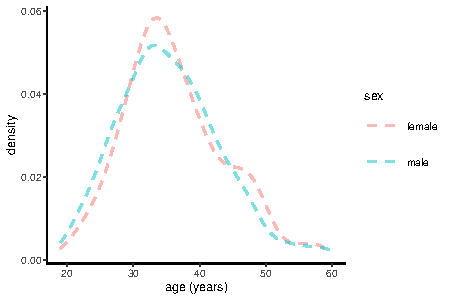
\includegraphics[width=\maxwidth]{figures/fig-fontsize-1} 
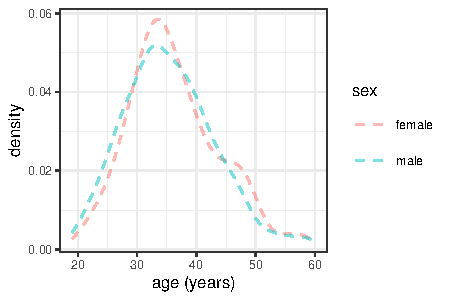
\includegraphics[width=\maxwidth]{figures/fig-fontsize-2} 

}



\end{knitrout}
\fi

\section{Getting Help in RStudio}

\subsection{The \RStudio\ help system}
There are several ways to get \RStudio\ to help you when you forget something.
Most objects in packages have help files that you can access by typing something 
like:
\begin{knitrout}
\definecolor{shadecolor}{rgb}{0.969, 0.969, 0.969}\color{fgcolor}\begin{kframe}
\begin{alltt}
\hlopt{?}\hlstd{bargraph}
\hlopt{?}\hlstd{histogram}
\hlopt{?}\hlstd{HELPrct}
\end{alltt}
\end{kframe}
\end{knitrout}
You can search the help system using
\begin{knitrout}
\definecolor{shadecolor}{rgb}{0.969, 0.969, 0.969}\color{fgcolor}\begin{kframe}
\begin{alltt}
\hlkwd{help.search}\hlstd{(}\hlstr{'Grand Rapids'}\hlstd{)}    \hlcom{# Does R know anything about Grand Rapids?}
\end{alltt}
\end{kframe}
\end{knitrout}
This can be useful if you don't know the name of the function or data set you 
are looking for.

\subsection{Tab completion}
As you type the name of a function in \RStudio, you can hit the tab key and it
will show you a list of all the ways you could complete that name, and after
you type the opening parenthesis, if you hit the tab key, you will get a list
of all the arguments and (sometimes) some helpful hints about what they are.)

\subsection{History}
If you know you have done something before, but can't remember how, you can
search your history.  The history tab shows a list of recently executed
commands.  There is also a search bar to help you find things from longer ago.

\subsection{Error messages}
When things go wrong, \R\ tries to help you out by providing an error message.
If you can't make sense of the message, you can try copying and pasting your
command and the error message and sending to me in an email.  One common error
message is illustrated below.
\begin{knitrout}
\definecolor{shadecolor}{rgb}{0.969, 0.969, 0.969}\color{fgcolor}\begin{kframe}
\begin{alltt}
\hlstd{fred} \hlkwb{<-} \hlnum{23}
\hlstd{frd}
\end{alltt}


{\ttfamily\noindent\bfseries\color{errorcolor}{\#\# Error in eval(expr, envir, enclos): object 'frd' not found}}\end{kframe}
\end{knitrout}
The object \code{frd} is not found because it was mistyped.  It should have
been \code{fred}.  If you see an ``object not found'' message, check your
typing and check to make sure that the necessary packages have been loaded.

\section{Graphical Summaries -- Important Ideas}

\subsection{The Most Important Template}

The plots we have created have all followed a single template

\begin{center}
	\Large 
	\texttt{ \fbox{\texttt{ goal }} ( \fbox{\texttt{ formula }}, data = \fbox{\texttt{ mydata }}, ... ) }
\end{center}
We will see this same template used again for numerical summaries and linear and non-linear 
modeling as well, so it is is important to master it.

\begin{itemize}
	\item \texttt{goal}: The name of the function generally describes your goal, 
		the thing you want the computer to produce for you.  In the case of plotting,
		it is the name of the plot.  When we do numerical summaries it will be the 
		name of the numerical summary (mean, median, etc.).
	\item
		\texttt{formula}: For plotting, the formula describes which variables are 
		used on the x-axis, the y-axis and for conditioning.  The general scheme is
\begin{knitrout}
\definecolor{shadecolor}{rgb}{0.969, 0.969, 0.969}\color{fgcolor}\begin{kframe}
\begin{alltt}
\hlstd{y} \hlopt{~} \hlstd{x} \hlopt{|} \hlstd{z}
\end{alltt}
\end{kframe}
\end{knitrout}
		where \texttt{z} is the conditioning variable.  Sometimes \texttt{y} or \texttt{z} 
		are missing (but the right-hand side \texttt{x} must always be included in a formula).
	\item
		\texttt{mydata:} A data frame must be given in which the variables mentioned in
		the formula can be found.  Variables not found there will be looked for in the 
		enclosing environment.  Sometimes we will take advantage of this to avoid creating
		a temporary data frame just to make a quick plot, but generally it is best to have
		all the information inside a data frame.
	\item
	\texttt{...} There are many optional arguments to control sizes, colors, etc.
	We will introduce these as they are needed. Consult the help files for assistance.
		
\end{itemize}

Just fill in the boxes and get your plot.

\subsection{Patterns and Deviations from Patterns}
The goal of a statistical plot is to help us see 
\begin{itemize}
\item 
potential patterns in the data, and 
\item
deviations from those patterns.  
\end{itemize}

\subsection{Different Plots for Different Kinds of Variables}
Graphical summaries can help us see the \emph{distribution} of a variable 
or the \emph{relationships} between two (or more) variables.  The type of plot
used will depend on the kinds of variables involved.
There is a nice summary of these on page~48.  You can use \function{demo()} to see how
to get \R\ to make the plots in this section.

Later, when we do statistical analysis, we will see that the analysis we use will 
also depend on the kinds of variables involved, so this is an important idea.

\subsection{Side-by-side Plots and Overlays Can Reveal Importance of Additional Factors}
The \pkg{ggformula} graphics plots make it particularly easy to generate plats that 
divide the data into groups and either produce a panel for each group (using \verb!|!)
or display each group in a different way (different colors or symbols, using 
the \argument{groups} argument).  These plots can reveal the 
possible influence of additional variables -- sometimes called covariates.

\subsection{Area = (relative) frequency}

Many plots are based on the key idea that our eyes are good at comparing areas.  Plots 
that use area (e.g., histograms, mosaic plots, bar charts, pie charts) should always obey
this principle
\begin{center}
\large
Area $ = $ (relative) frequency
\end{center}
Plots that violate this principle can be deceptive and distort the true nature
of the data.  

% \subsubsection*{An Example: Histogram with unequal bin widths}
% 
% It is possible to make histograms with bins that have different widths.
% But in this case it is important that the height of the bars is chosen so 
% that area (\emph{NOT height}) is proportional to frequency.  
% Using height instead of area would distort the picture.
% 
% When unequal bin sizes are specified, \function{histogram()} by default chooses
% the density scale:
% 
% <<hist-unequal-bins,fig.width = 3,fig.height = 2>>=
% gf_histogram( ~ Sepal.Length, data = iris, breaks = c(4,5,5.5,5.75,6,6.5,7,8,9))
% @
% The density scale is important.
% It tells \R\ to use a scale such that 
% the area (height $\times$ width) of the rectangles is equal to the relative frequency.
% For example, the bar from 5.0 to 5.5 has width $\frac12$ and height about $0.36$, so 
% the area is $0.18$, which means approximately 18\% of the sepal lengths are 
% between 5.0 and 5.5.
% 
% 
% It would be incorrect to choose \option{type = "count"} or \option{type = "proportion"} since
% this distorts the picture of the data.  Fortunately, \R\ will warn you if you try:
% <<hist-unequal-bins-bad-echo,fig.width = 3,fig.height = 2,eval = FALSE>>=
% histogram( ~ Sepal.Length, data = iris, breaks = c(4,5,5.5,5.75,6,6.5,7,8,9), type = 'count')
% @
% <<hist-unequal-bins-bad,fig.width = 3,fig.height = 2,echo = FALSE>>=
% trellis.par.set(theme = col.fastR2(bw = T))
% histogram( ~ Sepal.Length, data = iris, breaks = c(4,5,5.5,5.75,6,6.5,7,8,9),type = "count")
% trellis.focus('panel',1,1)
% grid.text(y = .7,'Never do this!', gp = gpar(col = 'red',cex = 2,alpha = .6))
% trellis.unfocus()
% trellis.par.set(theme = col.mosaic())
% @
% 
% Notice how different this looks.  Now the heights are equal to the relative
% frequency, but this makes the wider bars have too much area.


\section{Exercises}

The solutions to these exercises should be done using an RMarkdown document
and knitTHML in RStudio.
Include both the plots and the code you used to make them as well as any
required discussion.  Once you get the plots figured out, feel free to 
use some of the bells and whistles to make the plots even better.

\begin{problem}
	Create a scatterplot using the two variables in the \dataframe{oldfaith}
	data frame (available in the \pkg{alr4} package).  
	What do we learn about Old Faithful eruptions from this plot?
\end{problem}


\begin{problem}
	Where do the data in the \dataframe{CPS85} data frame (in the 
	\pkg{mosaic} package) come from?  What are the observational 
	units?  How many are there?
\end{problem}

\begin{problem}
	Choose a quantitative variable that interests you in the \dataframe{CPS85}
	data set.  Make an appropriate plot and comment on what you see.
\end{problem}

\begin{problem}
	Choose a categorical variable that interests you in the \dataframe{CPS85}
	data set.  Make an appropriate plot and comment on what you see.
\end{problem}

\begin{problem}
	Create a plot that displays two or more variables from the 
	\dataframe{CPS85} data.  At least one should be quantitative 
	and at least one should be categorical.
	Comment on what you can learn from your plot.
\end{problem}

\begin{problem}
	Where do the data in the \dataframe{mpg} data frame (in the 
	\pkg{ggplot2} package) come from?  What are the observational 
	units?  How many are there?
\end{problem}

\begin{problem}
	Choose a quantitative variable that interests you in the \dataframe{mpg}
	data set.  Make an appropriate plot and comment on what you see.
\end{problem}

\begin{problem}
	Choose a categorical variable that interests you in the \dataframe{mpg}
	data set.  Make an appropriate plot and comment on what you see.
\end{problem}

\begin{problem}
	Create a plot that displays two or more variables from the 
	\dataframe{mpg} data.  At least one should be quantitative 
	and at least one should be categorical.
	Comment on what you can learn from your plot.
\end{problem}

\begin{problem}The file at \url{http://www.calvin.edu/~rpruim/data/Fires.csv}
	is a csv file containing data on wild lands fires in the US over a number of years.
You can load this data one of two ways.
\begin{itemize}
	\item
		Go to the workspace tab, select \tab{Import Data Set}, choose \tab{From Web URL...}
		and follow the instructions.
	\item
		Use the following command in \R:
		
\begin{knitrout}
\definecolor{shadecolor}{rgb}{0.969, 0.969, 0.969}\color{fgcolor}\begin{kframe}
\begin{alltt}
\hlcom{# equivalent to "From Text (base)" in RStudio}
\hlstd{Fires} \hlkwb{<-} \hlkwd{read.csv}\hlstd{(}\hlstr{"https://rpruim.github.io/Engineering-Statistics/data/Fires.csv"}\hlstd{)}

\hlcom{# alternative method -- equivalent to "From Text (readr)" in RStudio}
\hlkwd{library}\hlstd{(readr)}
\hlstd{Fires} \hlkwb{<-} \hlkwd{read_csv}\hlstd{(}\hlstr{"https://rpruim.github.io/Engineering-Statistics/data/Fires.csv"}\hlstd{)}
\end{alltt}


{\ttfamily\noindent\itshape\color{messagecolor}{\#\# \\\#\# -- Column specification ------------------------------------------------------------------\\\#\# cols(\\\#\#\ \  Year = col\_double(),\\\#\#\ \  Fires = col\_double(),\\\#\#\ \  Acres = col\_double()\\\#\# )}}\end{kframe}
\end{knitrout}
\end{itemize}
You can also use either of these methods to read from a file rather than from a
web URL, so this is a good way to get your own data into \R.
\begin{enumerate}
	\item
		The source for these data claim that data before a certain year should not be compared
		to data from after that year because the older data were computed a different way and
		are not considered as reliable.  What year is the break point?  Use graphs of the data 
		over time to estimate when something changed.
	\item
		You can trim the data to just the subset you want using \function{subset()}.  For 
		example, to get just the subset of years since 1966, you would use
\begin{knitrout}
\definecolor{shadecolor}{rgb}{0.969, 0.969, 0.969}\color{fgcolor}\begin{kframe}
\begin{alltt}
\hlstd{Fires2} \hlkwb{<-} \hlkwd{subset}\hlstd{(Fires, Year} \hlopt{>} \hlnum{1966}\hlstd{)}
\end{alltt}
\end{kframe}
\end{knitrout}
		Be sure to use a new name if you want to keep the original data available.

		Do this to create a data set that contains only the data from the new data regime (based on your answer in the previous problem).
	\item
		Using only the data from this smaller set, how would describe what is happening with 
		fires over time?
\end{enumerate}
\end{problem}

\begin{problem}
	Use \R's help system to find out what the \variable{i1} and \variable{i2}
	variables are in the \dataframe{HELPrct} data frame.  Make histograms
	for each variable and comment on what you find out.  How would you describe
	the shape of these distributions?  Do you see any outliers (observations
	that don't seem to fit the pattern of the rest of the data)?  
\end{problem}
\begin{problem}
	Compare the distributions of \variable{i1} and \variable{i2} among men
	and women.
\end{problem}
\begin{solution}
\begin{knitrout}
\definecolor{shadecolor}{rgb}{0.969, 0.969, 0.969}\color{fgcolor}\begin{kframe}
\begin{alltt}
\hlkwd{gf_dens}\hlstd{(} \hlopt{~}\hlstd{max_drinks,} \hlkwc{color} \hlstd{=} \hlopt{~} \hlstd{sex,} \hlkwc{data} \hlstd{= HELPrct )}
\hlkwd{gf_dens}\hlstd{(} \hlopt{~}\hlstd{avg_drinks,} \hlkwc{color} \hlstd{=} \hlopt{~} \hlstd{sex,} \hlkwc{data} \hlstd{= HELPrct )}
\end{alltt}
\end{kframe}

{\centering 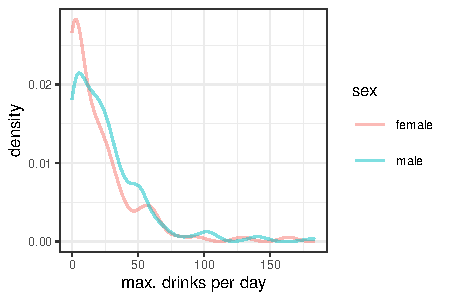
\includegraphics[width=\maxwidth]{figures/fig-unnamed-chunk-26-1} 
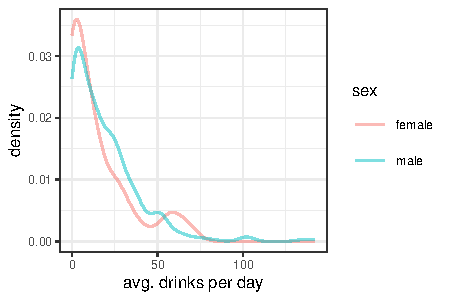
\includegraphics[width=\maxwidth]{figures/fig-unnamed-chunk-26-2} 

}



\end{knitrout}
\end{solution}

\begin{problem}
	Compare the distributions of \variable{i1} and \variable{i2} among 
	the three \variable{substance} groups.
\end{problem}
\begin{solution}
\begin{knitrout}
\definecolor{shadecolor}{rgb}{0.969, 0.969, 0.969}\color{fgcolor}\begin{kframe}
\begin{alltt}
\hlkwd{gf_dens}\hlstd{(} \hlopt{~}\hlstd{i1,} \hlkwc{color} \hlstd{=} \hlopt{~} \hlstd{substance,} \hlkwc{data} \hlstd{= HELPrct )}
\hlkwd{gf_dens}\hlstd{(} \hlopt{~}\hlstd{i2,} \hlkwc{color} \hlstd{=} \hlopt{~} \hlstd{substance,} \hlkwc{data} \hlstd{= HELPrct )}
\end{alltt}
\end{kframe}

{\centering 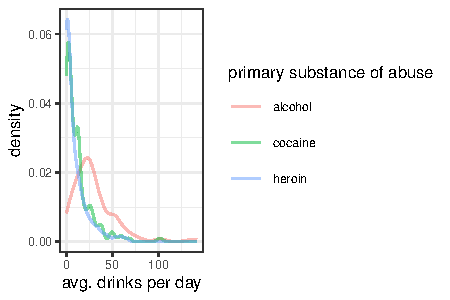
\includegraphics[width=\maxwidth]{figures/fig-unnamed-chunk-27-1} 
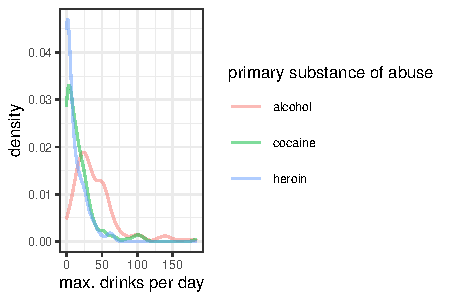
\includegraphics[width=\maxwidth]{figures/fig-unnamed-chunk-27-2} 

}



\end{knitrout}
\begin{knitrout}
\definecolor{shadecolor}{rgb}{0.969, 0.969, 0.969}\color{fgcolor}\begin{kframe}
\begin{alltt}
\hlkwd{gf_dens}\hlstd{(} \hlopt{~}\hlstd{i1} \hlopt{|} \hlstd{sex,} \hlkwc{color} \hlstd{=} \hlopt{~} \hlstd{substance,} \hlkwc{data} \hlstd{= HELPrct )}
\hlkwd{gf_dens}\hlstd{(} \hlopt{~}\hlstd{i2} \hlopt{|} \hlstd{sex,} \hlkwc{color} \hlstd{=} \hlopt{~} \hlstd{substance,} \hlkwc{data} \hlstd{= HELPrct )}
\end{alltt}
\end{kframe}

{\centering 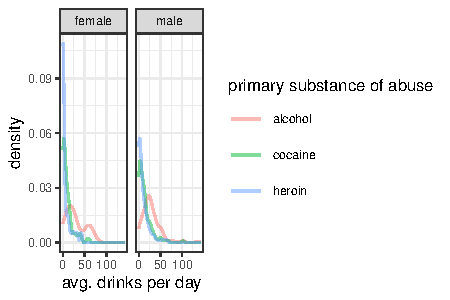
\includegraphics[width=\maxwidth]{figures/fig-unnamed-chunk-28-1} 
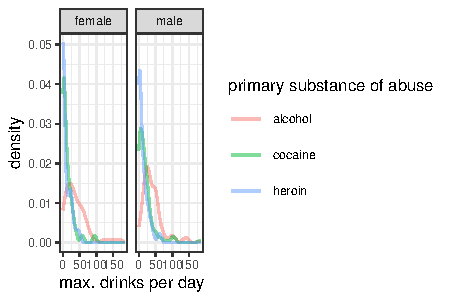
\includegraphics[width=\maxwidth]{figures/fig-unnamed-chunk-28-2} 

}



\end{knitrout}
\begin{knitrout}
\definecolor{shadecolor}{rgb}{0.969, 0.969, 0.969}\color{fgcolor}\begin{kframe}
\begin{alltt}
\hlkwd{gf_point}\hlstd{( i2} \hlopt{~} \hlstd{i1,} \hlkwc{color} \hlstd{=} \hlopt{~} \hlstd{sex,} \hlkwc{data} \hlstd{=  HELPrct,} \hlkwc{alpha} \hlstd{=} \hlnum{.6}\hlstd{,} \hlkwc{size} \hlstd{=} \hlnum{.6} \hlstd{)}
\end{alltt}
\end{kframe}

{\centering 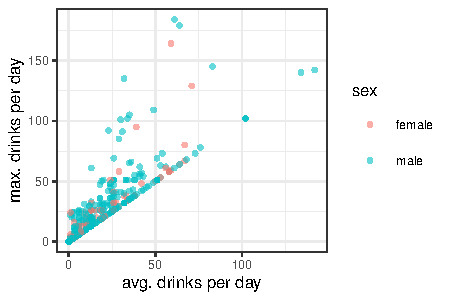
\includegraphics[width=\maxwidth]{figures/fig-unnamed-chunk-29-1} 

}



\end{knitrout}
\end{solution}

\begin{problem}
	The \dataframe{SnowGR} contains historical data on snowfall in Grand Rapids, MI.
	The snowfall total for January, 2014 was 36.6 inches.
	\begin{enumerate}
		\item
			Create a histogram of January snowfall totals.  How unusual is 36.6 inches of 
			snow in January?
		\item
			If there is a lot of snow in January, should we expect to have unusually much
			or little snow in February?  Make a scatter plot comparing January and February
			snowfall totals and comment on what you see there.
	\end{enumerate}
\end{problem}

\begin{solution}
\begin{knitrout}
\definecolor{shadecolor}{rgb}{0.969, 0.969, 0.969}\color{fgcolor}\begin{kframe}
\begin{alltt}
\hlkwd{gf_histogram}\hlstd{(} \hlopt{~} \hlstd{Jan,} \hlkwc{data} \hlstd{= SnowGR)}
\end{alltt}


{\ttfamily\noindent\color{warningcolor}{\#\# Warning: Removed 1 rows containing non-finite values (stat\_bin).}}\end{kframe}

{\centering 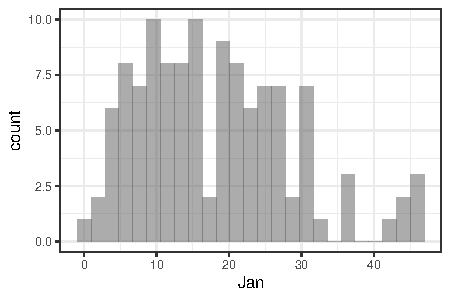
\includegraphics[width=\maxwidth]{figures/fig-unnamed-chunk-30-1} 

}



\end{knitrout}
36.6 inches is pretty high, but not the highest ever for a January.  Certainly well above average.

\begin{knitrout}
\definecolor{shadecolor}{rgb}{0.969, 0.969, 0.969}\color{fgcolor}\begin{kframe}
\begin{alltt}
\hlkwd{gf_point}\hlstd{(Feb} \hlopt{~} \hlstd{Jan,} \hlkwc{data} \hlstd{= SnowGR)}
\end{alltt}


{\ttfamily\noindent\color{warningcolor}{\#\# Warning: Removed 2 rows containing missing values (geom\_point).}}\end{kframe}

{\centering 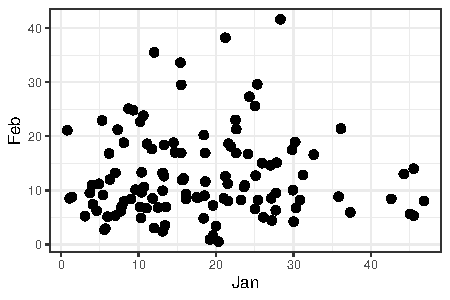
\includegraphics[width=\maxwidth]{figures/fig-unnamed-chunk-31-1} 

}



\end{knitrout}
There is no clear trend.  Somtime the snow keeps on coming, but a heavy snow
January could be followed by either a heavy or light snow February.
\end{solution}
\shipoutProblems

\ifsolutions
\ifsolutionslocal
\newpage
\section*{Solutions}
\shipoutSolutions
\fi
\fi




\Chapter{Numerical Summaries}

\section{Tabulating Data}
A table is one kind of numerical summary of a data set.  In fact, you can think of histograms
and bar graphs as graphical representations of summary tables.  But sometimes it is nice to
have the table itself.  \R\ provides several ways of obtaining such tables.

\subsection{Tabulating a categorical variable}

\subsubsection*{The formula interface}

There are several functions for tabulating categorical variables.  
\function{tally()}  uses a syntax that is very similar to \function{bargraph()}.    
We'll call this method the \term{formula interface}.
(\R\ calls anything with a tilde (\code{\~}) a formula.)
\Rindex{tally()}%
\Rindex{table()}%
\begin{knitrout}
\definecolor{shadecolor}{rgb}{0.969, 0.969, 0.969}\color{fgcolor}\begin{kframe}
\begin{alltt}
\hlkwd{tally}\hlstd{(} \hlopt{~} \hlstd{sex,} \hlkwc{data} \hlstd{= KidsFeet )}
\end{alltt}
\begin{verbatim}
## sex
##  B  G 
## 20 19
\end{verbatim}
\begin{alltt}
\hlkwd{tally}\hlstd{(} \hlopt{~} \hlstd{sex,} \hlkwc{data} \hlstd{= KidsFeet,} \hlkwc{format} \hlstd{=} \hlstr{"prop"} \hlstd{)}
\end{alltt}
\begin{verbatim}
## sex
##      B      G 
## 0.5128 0.4872
\end{verbatim}
\begin{alltt}
\hlkwd{tally}\hlstd{(} \hlopt{~} \hlstd{sex,} \hlkwc{data} \hlstd{= KidsFeet,} \hlkwc{format} \hlstd{=} \hlstr{"perc"} \hlstd{)}
\end{alltt}
\begin{verbatim}
## sex
##     B     G 
## 51.28 48.72
\end{verbatim}
\end{kframe}
\end{knitrout}

\subsubsection*{The \$-interface}
\function{table()} and its cousins use the \code{\$} operator which selects one variable 
out of a data frame.
\begin{knitrout}
\definecolor{shadecolor}{rgb}{0.969, 0.969, 0.969}\color{fgcolor}\begin{kframe}
\begin{alltt}
\hlstd{KidsFeet}\hlopt{$}\hlstd{sex}      \hlcom{# general syntax: dataframe$variable}
\end{alltt}
\begin{verbatim}
##  [1] B B B B B B B G G B B B B B G G G G G G B B G G G B G B B B G G G B B G G G G
## Levels: B G
\end{verbatim}
\begin{alltt}
\hlkwd{table}\hlstd{(KidsFeet}\hlopt{$}\hlstd{sex)}
\end{alltt}
\begin{verbatim}
## 
##  B  G 
## 20 19
\end{verbatim}
\begin{alltt}
\hlcom{# tally() is ambidextrous:}
\hlkwd{tally}\hlstd{(KidsFeet}\hlopt{$}\hlstd{sex)}
\end{alltt}
\begin{verbatim}
## X
##  B  G 
## 20 19
\end{verbatim}
\end{kframe}
\end{knitrout}
We'll call this interface the \code{\$}-interface.

\subsubsection*{Two interfaces}
Some functions in \R\ require the formula interface, some require the
\code{\$}-interface, and some allow you to use either one.%
\footnote{One of the things that the \pkg{mosaic} package does is provide a
formula interface for many functions that only had a \code{\$}-interface
before.}
% For example, histogram will also work like this.
% % gf_histogram( HELPrct$age )
% But notice that the output is not quite as nice, since the default label 
% for the horizontal axis now shows both the data frame name and the variable name
% with a \code{\$} between.  

\emph{My advice is to use formula interfaces whenever they are available and to choose
tools that make this possible.}

\subsection{Tabulating a quantitative variable}

Although \function{tally()} and \function{table()} work with quantitative variables
as well as categorical variables, this is only useful when there are not too
many different values for the variable.

\begin{knitrout}
\definecolor{shadecolor}{rgb}{0.969, 0.969, 0.969}\color{fgcolor}\begin{kframe}
\begin{alltt}
\hlkwd{tally}\hlstd{(} \hlopt{~}\hlstd{age,} \hlkwc{data} \hlstd{= HELPrct )}
\end{alltt}
\begin{verbatim}
## age
## 19 20 21 22 23 24 25 26 27 28 29 30 31 32 33 34 35 36 37 38 39 40 41 42 43 44 45 46 47 48 
##  1  2  3  8  5  8  7 13 18 15 18 18 20 28 35 18 25 23 20 18 27 10 20 10 13  7 13  5 14  5 
## 49 50 51 52 53 54 55 56 57 58 59 60 
##  8  2  1  1  3  1  2  1  2  2  2  1
\end{verbatim}
\end{kframe}
\end{knitrout}

\subsubsection*{Tabulating in bins (optional)}
Usually a graph is the best way to display and summarize quantitative data, but if you need to creat a summary table, you may need to group quantitative data into bins.  We just have to tell \R\ what the bins are.
For example, suppose we wanted to group the 20s, 30s, 40s, etc. together.
\Rindex{cut()}%
\Rindex{xtabs()}%
\Rindex{mtable()}%
\Rindex{table()}%
\begin{knitrout}
\definecolor{shadecolor}{rgb}{0.969, 0.969, 0.969}\color{fgcolor}\begin{kframe}
\begin{alltt}
\hlcom{# let's add a new variable to HELPrct}
\hlstd{HELPrct} \hlkwb{<-} \hlstd{HELPrct} \hlopt
  \hlkwd{mutate}\hlstd{(}\hlkwc{binnedAge} \hlstd{=} \hlkwd{cut}\hlstd{(age,} \hlkwc{breaks}\hlstd{=}\hlkwd{c}\hlstd{(}\hlnum{10}\hlstd{,}\hlnum{20}\hlstd{,}\hlnum{30}\hlstd{,}\hlnum{40}\hlstd{,}\hlnum{50}\hlstd{,}\hlnum{60}\hlstd{,}\hlnum{70}\hlstd{) ))}
\hlkwd{head}\hlstd{(HELPrct)}
\end{alltt}
\begin{verbatim}
##   age anysubstatus anysub cesd d1 daysanysub dayslink drugrisk e2b female    sex g1b
## 1  37            1    yes   49  3        177      225        0  NA      0   male yes
## 2  37            1    yes   30 22          2       NA        0  NA      0   male yes
## 3  26            1    yes   39  0          3      365       20  NA      0   male  no
## 4  39            1    yes   15  2        189      343        0   1      1 female  no
## 5  32            1    yes   39 12          2       57        0   1      0   male  no
## 6  47            1    yes    6  1         31      365        0  NA      1 female  no
##   homeless i1 i2 id indtot linkstatus link    mcs   pcs pss_fr racegrp satreat sexrisk
## 1   housed 13 26  1     39          1  yes 25.112 58.41      0   black      no       4
## 2 homeless 56 62  2     43         NA <NA> 26.670 36.04      1   white      no       7
## 3   housed  0  0  3     41          0   no  6.763 74.81     13   black      no       2
## 4   housed  5  5  4     28          0   no 43.968 61.93     11   white     yes       4
## 5 homeless 10 13  5     38          1  yes 21.676 37.35     10   black      no       6
## 6   housed  4  4  6     29          0   no 55.509 46.48      5   black      no       5
##   substance treat avg_drinks max_drinks hospitalizations binnedAge
## 1   cocaine   yes         13         26                3   (30,40]
## 2   alcohol   yes         56         62               22   (30,40]
## 3    heroin    no          0          0                0   (20,30]
## 4    heroin    no          5          5                2   (30,40]
## 5   cocaine    no         10         13               12   (30,40]
## 6   cocaine   yes          4          4                1   (40,50]
\end{verbatim}
\begin{alltt}
\hlkwd{tally}\hlstd{(} \hlopt{~} \hlstd{binnedAge,} \hlkwc{data} \hlstd{= HELPrct)}
\end{alltt}
\begin{verbatim}
## binnedAge
## (10,20] (20,30] (30,40] (40,50] (50,60] (60,70] 
##       3     113     224      97      16       0
\end{verbatim}
\end{kframe}
\end{knitrout}
That's not quite what we wanted: 30 is in with the 20s, for example.
Here's how we fix that.

\begin{knitrout}
\definecolor{shadecolor}{rgb}{0.969, 0.969, 0.969}\color{fgcolor}\begin{kframe}
\begin{alltt}
\hlstd{HELPrct} \hlkwb{<-} \hlstd{HELPrct} \hlopt
  \hlkwd{mutate}\hlstd{(}\hlkwc{binnedAge} \hlstd{=} \hlkwd{cut}\hlstd{(age,} \hlkwc{breaks}\hlstd{=}\hlkwd{c}\hlstd{(}\hlnum{10}\hlstd{,}\hlnum{20}\hlstd{,}\hlnum{30}\hlstd{,}\hlnum{40}\hlstd{,}\hlnum{50}\hlstd{,}\hlnum{60}\hlstd{,}\hlnum{70}\hlstd{),} \hlkwc{right}\hlstd{=}\hlnum{FALSE}\hlstd{) )}
\hlkwd{tally}\hlstd{(} \hlopt{~} \hlstd{binnedAge,} \hlkwc{data} \hlstd{= HELPrct )}
\end{alltt}
\begin{verbatim}
## binnedAge
## [10,20) [20,30) [30,40) [40,50) [50,60) [60,70) 
##       1      97     232     105      17       1
\end{verbatim}
\end{kframe}
\end{knitrout}


We won't use this very often, since typically seeing this information in a histogram is 
more useful.  


\subsection{Cross-tables: Tabulating two or more variables}

\function{tally()} can also compute cross tables for two (or more) variables.
\begin{knitrout}
\definecolor{shadecolor}{rgb}{0.969, 0.969, 0.969}\color{fgcolor}\begin{kframe}
\begin{alltt}
\hlkwd{tally}\hlstd{(sex} \hlopt{~} \hlstd{substance,} \hlkwc{data}\hlstd{=HELPrct)}
\end{alltt}
\begin{verbatim}
##         substance
## sex      alcohol cocaine heroin
##   female      36      41     30
##   male       141     111     94
\end{verbatim}
\begin{alltt}
\hlkwd{tally}\hlstd{(}\hlopt{~} \hlstd{sex} \hlopt{+} \hlstd{substance,} \hlkwc{data}\hlstd{=HELPrct)}
\end{alltt}
\begin{verbatim}
##         substance
## sex      alcohol cocaine heroin
##   female      36      41     30
##   male       141     111     94
\end{verbatim}
\end{kframe}
\end{knitrout}

\section{Working with Pre-Tabulated Data}

Sometimes data arrive pre-tabulated.  We can use \function{gf_col()} instead
of \function{gf_bar()} to graph pre-tabulated data.

\begin{knitrout}
\definecolor{shadecolor}{rgb}{0.969, 0.969, 0.969}\color{fgcolor}\begin{kframe}
\begin{alltt}
\hlkwd{library}\hlstd{(abd)}           \hlcom{# data sets from Analysis of Biological Data}
\hlstd{TeenDeaths}
\end{alltt}
\begin{verbatim}
##                          cause deaths
## 1                    Accidents   6688
## 2                     Homicide   2093
## 3                      Suicide   1615
## 4              Malignant tumor    745
## 5                Heart disease    463
## 6     Congenital abnormalities    222
## 7  Chronic respiratory disease    107
## 8      Influenza and pneumonia     73
## 9     Cerebrovascular diseases     67
## 10                 Other tumor     52
## 11            All other causes   1653
\end{verbatim}
\begin{alltt}
\hlkwd{gf_col}\hlstd{(deaths} \hlopt{~} \hlstd{cause,} \hlkwc{data}\hlstd{=TeenDeaths)} \hlopt
  \hlkwd{gf_refine}\hlstd{(}\hlkwd{coord_flip}\hlstd{())}
\end{alltt}
\end{kframe}

{\centering 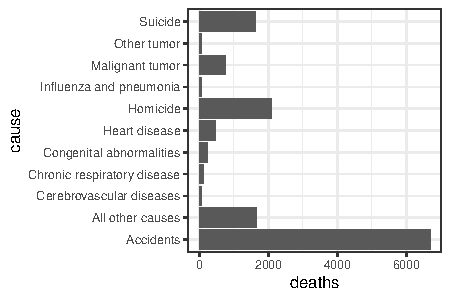
\includegraphics[width=\maxwidth]{figures/fig-teen-deaths-1} 

}



\end{knitrout}

Notice that by default the causes are displayed in alphabetical order.  
\R\ assumes that categorical data is nominal 
(that is, there is no particular natural or logical ordering to the categories) 
unless you say otherwise.

Here is an easy way to have things appear in a different order. The causes of death are reordered in order of increasing number of \variable{deaths} caused.
\begin{knitrout}
\definecolor{shadecolor}{rgb}{0.969, 0.969, 0.969}\color{fgcolor}\begin{kframe}
\begin{alltt}
\hlkwd{gf_col}\hlstd{( deaths} \hlopt{~} \hlkwd{reorder}\hlstd{(cause, deaths),} \hlkwc{data} \hlstd{= TeenDeaths)} \hlopt
  \hlkwd{gf_refine}\hlstd{(}\hlkwd{coord_flip}\hlstd{())} \hlopt
  \hlkwd{gf_labs}\hlstd{(}\hlkwc{x} \hlstd{=} \hlstr{'Cause of Death'}\hlstd{,} \hlkwc{y} \hlstd{=} \hlstr{'Number of Deaths'}\hlstd{)}
\end{alltt}
\end{kframe}

{\centering 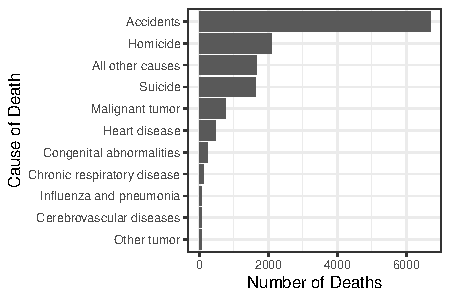
\includegraphics[width=\maxwidth]{figures/fig-teen-deaths-order-1} 

}



\end{knitrout}


\section{Summarizing Distributions of Quantitative Variables}
\subsubsection*{Important Note}
Numerical summaries are a convenient way to 
describe a distribution, but remember that numerical summaries 
do not necessarily tell you everything there is to know about a distribution.  When working with a new dataset, it is \emph{always} important to explore the data as fully as possible (commonly including graphical as well as numerical summaries, and sometimes even examining the data table directly) before accepting any simplified summary as a good representation of the data.  You might discover certain patterns in the data, interesting features, or even outliers or mistakes in the data, that make certain summaries misrepresentations of the whole.

\subsubsection*{Notation}
In statistics $n$ (or sometimes $N$) almost always means the number 
of observations (i.e., the number of rows in a data frame).

If $y$ is a variable in a data set with $n$ cases, we 
can denote the $n$ values of $y$ as 
\begin{itemize}
\item
$y_1, y_2, y_3, \dots, y_n$ (in the original order of the data).
\item
$y_{(1)}, y_{(2)}, y_{(3)}, \dots y_{(n)}$ (in sorted order from smallest to largest).

\end{itemize}

The symbol $\displaystyle \sum$ represents summation (adding up a bunch of values).

\section{Measures of Center}
Measures of center attempt to give us a sense of what is a
typical value for the distribution.

%\subsection{Mean}

\begin{align*}
\mbox{mean of $y$} 
&=
\mean{y}
= \frac{\displaystyle \sum_{i = 1}^{n} y_i}{n}
= \frac{\mbox{sum of values}}{\mbox{number of values}}  
\\[3mm]
\mbox{median of $y$}
&=
\mbox{the ``middle'' number (after putting the numbers in increasing order)
} 
\end{align*}

\begin{itemize}
\item
The mean is the ``balancing point'' of the distribution.
\item
The median\footnote{A note about calculating medians: If the number of datapoints is odd, the median is the middle value (after putting the observations in increasing order). In cases where there is an even number of observations, the median is the
  average of the middle two observations.} is the 50th percentile: half of the distribution is below the median,
half is above.
\item
If the distribution is symmetric, then the mean and median are the same.
\item
In a skewed distribution, the mean is pulled farther toward the tail than the median is.
\item
\emph{A few very large or very small values can change the mean a lot,}
so the mean is \term{sensitive to outliers} and is a better measure of center
when the distribution is symmetric than when it is skewed.
\item
The median is a \term{resistant measure} (resistant to the presence of outlier) -- it is not affected much by a few very large or very small values.
\end{itemize}


%\subsection{Median}

\section{Measures of Spread}

\begin{align*}
\mbox{variance of $y$} 
= s^2_y 
&= 
\frac{\displaystyle \sum_{i = 1}^{n} (y_i - \mean y)^2 }{n-1}
\\[4mm]
\mbox{standard deviaiton of $y$} = s_y 
&= \sqrt{s^2_y} 
\\
&= \mbox{square root of variance}
\\[4mm]
\mbox{interquartile range} = \mbox{IQR}
&= Q_3 - Q_1 
\\
& = \mbox{difference between first and third quartiles (defined shortly)}
\end{align*}

\begin{itemize}
\item
Roughly, the standard deviation is the ``average deviation from the mean".  (That's not
exactly right because of the squaring involved and because we are dividing
by $n-1$ instead of by $n$.  More on that denominator later.)  
\item
The mean and standard deviation are especially useful for describing 
\term{normal distributions} and other unimodal, symmetric distributions that
are roughly ``bell-shaped''.  (We'll learn more about normal distributions later.)
\item
Like the mean, the variance and standard deviation are 
sensitive to outliers and less suited for summarizing skewed distributions.
\item
It is perhaps of some value to compute the variance and standard deviation by hand
once or twice to make sure you understand how these measures are defined, but we will
typically let \R\ do the calculations for us.
\end{itemize}

To get a numerical summary of a variable (a statistic), we need to tell 
\R\ which statistic we want and the variable and data frame involved.  
There several ways we can do this in \R.  
Here are several ways to get the mean, for example:
\Rindex{mean()}%
\begin{knitrout}
\definecolor{shadecolor}{rgb}{0.969, 0.969, 0.969}\color{fgcolor}\begin{kframe}
\begin{alltt}
\hlkwd{mean}\hlstd{(HELPrct}\hlopt{$}\hlstd{age)}            \hlcom{# this is the old fashioned way}
\end{alltt}
\begin{verbatim}
## [1] 35.65
\end{verbatim}
\begin{alltt}
\hlkwd{mean}\hlstd{(}\hlopt{~} \hlstd{age,} \hlkwc{data} \hlstd{= HELPrct)}  \hlcom{# similar to our plotting methods; only works for some functions}
\end{alltt}
\begin{verbatim}
## [1] 35.65
\end{verbatim}
\begin{alltt}
\hlkwd{df_stats}\hlstd{(}\hlopt{~} \hlstd{age,} \hlkwc{data} \hlstd{= HELPrct, mean)}  \hlcom{# formula-based and very flexible}
\end{alltt}
\begin{verbatim}
##   response  mean
## 1      age 35.65
\end{verbatim}
\end{kframe}
\end{knitrout}
Using the formula style, we can now compute several different statistics.
\Rindex{sd()}%
\Rindex{var()}%
\begin{knitrout}
\definecolor{shadecolor}{rgb}{0.969, 0.969, 0.969}\color{fgcolor}\begin{kframe}
\begin{alltt}
\hlkwd{mean}\hlstd{(} \hlopt{~} \hlstd{age,} \hlkwc{data} \hlstd{= HELPrct)}
\end{alltt}
\begin{verbatim}
## [1] 35.65
\end{verbatim}
\begin{alltt}
\hlkwd{sd}\hlstd{(} \hlopt{~} \hlstd{age,} \hlkwc{data} \hlstd{= HELPrct)}
\end{alltt}
\begin{verbatim}
## [1] 7.71
\end{verbatim}
\begin{alltt}
\hlkwd{var}\hlstd{(} \hlopt{~} \hlstd{age,} \hlkwc{data} \hlstd{= HELPrct)}
\end{alltt}
\begin{verbatim}
## [1] 59.45
\end{verbatim}
\end{kframe}
\end{knitrout}
\Rindex{median()}%
\Rindex{IQR()}%
\Rindex{df_stats()}%
\begin{knitrout}
\definecolor{shadecolor}{rgb}{0.969, 0.969, 0.969}\color{fgcolor}\begin{kframe}
\begin{alltt}
\hlkwd{median}\hlstd{(} \hlopt{~} \hlstd{age,} \hlkwc{data} \hlstd{= HELPrct)}
\end{alltt}
\begin{verbatim}
## [1] 35
\end{verbatim}
\begin{alltt}
\hlkwd{IQR}\hlstd{(} \hlopt{~} \hlstd{age,} \hlkwc{data} \hlstd{= HELPrct)}
\end{alltt}
\begin{verbatim}
## [1] 10
\end{verbatim}
\begin{alltt}
\hlkwd{df_stats}\hlstd{(} \hlopt{~} \hlstd{age,} \hlkwc{data} \hlstd{= HELPrct)}  \hlcom{# this computes several statistics at once}
\end{alltt}
\begin{verbatim}
##   response min Q1 median Q3 max  mean   sd   n missing
## 1      age  19 30     35 40  60 35.65 7.71 453       0
\end{verbatim}
\end{kframe}
\end{knitrout}

It is also possible to compute these statistics separately for each of several groups.
The syntax is much like the the syntax we used when plotting.  In fact, we have two 
choices for the formula:  \verb!y ~ x! or \verb! ~ x | z!.

\begin{knitrout}
\definecolor{shadecolor}{rgb}{0.969, 0.969, 0.969}\color{fgcolor}\begin{kframe}
\begin{alltt}
\hlkwd{mean}\hlstd{(age} \hlopt{~} \hlstd{sex,} \hlkwc{data} \hlstd{= HELPrct)}
\end{alltt}
\begin{verbatim}
## female   male 
##  36.25  35.47
\end{verbatim}
\begin{alltt}
\hlkwd{sd}\hlstd{(age} \hlopt{~} \hlstd{sex,} \hlkwc{data} \hlstd{= HELPrct)}
\end{alltt}
\begin{verbatim}
## female   male 
##  7.585  7.750
\end{verbatim}
\begin{alltt}
\hlkwd{df_stats}\hlstd{(} \hlopt{~} \hlstd{age} \hlopt{|} \hlstd{sex,} \hlkwc{data} \hlstd{= HELPrct )}
\end{alltt}
\begin{verbatim}
##   response    sex min Q1 median   Q3 max  mean    sd   n missing
## 1      age female  21 31     35 40.5  58 36.25 7.585 107       0
## 2      age   male  19 30     35 40.0  60 35.47 7.750 346       0
\end{verbatim}
\end{kframe}
\end{knitrout}

\subsection{A word of caution}
None of these measures (especially the mean and median) 
is a particularly good summary of a distribution if the distribution is not unimodal.  
The histogram below shows the lengths of eruptions of the Old Faithful geyser
at Yellowstone National Park.
\begin{knitrout}
\definecolor{shadecolor}{rgb}{0.969, 0.969, 0.969}\color{fgcolor}\begin{kframe}
\begin{alltt}
\hlkwd{df_stats}\hlstd{(}\hlopt{~} \hlstd{Duration,} \hlkwc{data} \hlstd{= oldfaith)}
\end{alltt}
\begin{verbatim}
##   response min  Q1 median    Q3 max  mean    sd   n missing
## 1 Duration  96 130    240 267.8 306 209.9 68.39 270       0
\end{verbatim}
\begin{alltt}
\hlkwd{gf_histogram}\hlstd{(} \hlopt{~} \hlstd{Duration,} \hlkwc{data} \hlstd{= oldfaith,}  \hlkwc{bins} \hlstd{=} \hlnum{20}\hlstd{)} \hlopt
        \hlkwd{gf_labs}\hlstd{(}\hlkwc{title} \hlstd{=} \hlstr{"Old Faithful Eruption Times"}\hlstd{,} \hlkwc{x} \hlstd{=} \hlstr{"duration (sec)"}\hlstd{)}
\end{alltt}
\end{kframe}

{\centering 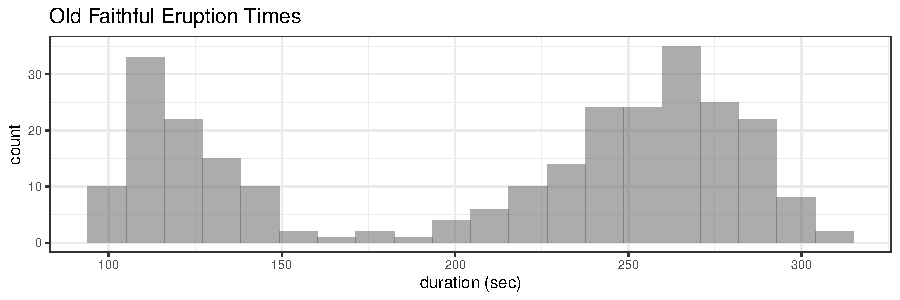
\includegraphics[width=\maxwidth]{figures/fig-faithful-1} 

}



\end{knitrout}
Notice that the mean and median do not represent typical eruption times very well.  
Nearly all eruptions are either quite a bit shorter or quite a bit longer.  
(This is especially true of the mean.)


\subsection{Box plots}

Boxplots (also called box-and-whisker plots) are a graphical representation of a 
\term{5-number summary} of a quantitative variable.  The five numbers are
the five \term{quantiles}:
\begin{itemize}
	\item $Q_0$, the minimum
	\item $Q_1$, the first quartile (25th percintile) 
	\item $Q_2$, the median (50th percentile)
	\item $Q_3$, the third quartile (75th percentile)
	\item $Q_4$, the maximum
\end{itemize}
\begin{knitrout}
\definecolor{shadecolor}{rgb}{0.969, 0.969, 0.969}\color{fgcolor}\begin{kframe}
\begin{alltt}
\hlkwd{gf_boxplot}\hlstd{(}\hlopt{~}\hlstd{age,} \hlkwc{data}\hlstd{=HELPrct)}
\end{alltt}
\end{kframe}

{\centering 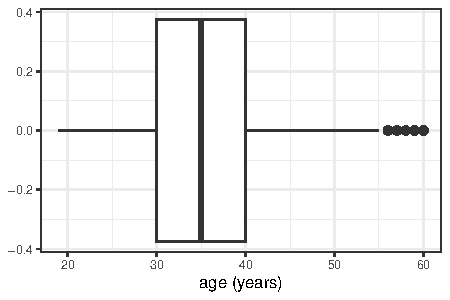
\includegraphics[width=\maxwidth]{figures/fig-bwplot-1} 

}



\end{knitrout}

Boxplots provide a way of comparing multiple groups that is especially informative and visually effective.  Here is one way to make boxplots of multiple groups (it 
should look familiar from what we know about histogram):
\begin{knitrout}
\definecolor{shadecolor}{rgb}{0.969, 0.969, 0.969}\color{fgcolor}\begin{kframe}
\begin{alltt}
\hlkwd{gf_boxplot}\hlstd{(}\hlopt{~}\hlstd{age} \hlopt{|} \hlstd{substance,} \hlkwc{data}\hlstd{=HELPrct)}
\end{alltt}
\end{kframe}

{\centering 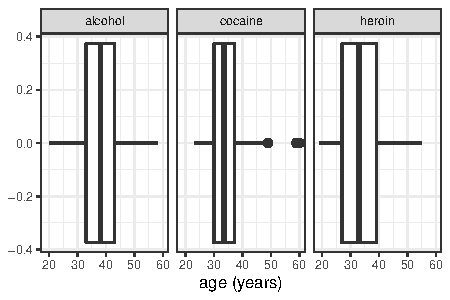
\includegraphics[width=\maxwidth]{figures/fig-bwplot1-1} 

}



\end{knitrout}
But \function{gf_boxplot()} has a better way.  Put the quantitative variable on one side of the
wiggle and the categorical on the other.  The placement determines which goes along the 
vertical axis and which along the horizontal axis -- just like it did for \function{gf_point()}.
\begin{knitrout}
\definecolor{shadecolor}{rgb}{0.969, 0.969, 0.969}\color{fgcolor}\begin{kframe}
\begin{alltt}
\hlkwd{gf_boxplot}\hlstd{(substance} \hlopt{~} \hlstd{age,} \hlkwc{data}\hlstd{=HELPrct)}
\hlkwd{gf_boxplot}\hlstd{(age} \hlopt{~} \hlstd{substance,} \hlkwc{data}\hlstd{=HELPrct)}
\end{alltt}
\end{kframe}

{\centering 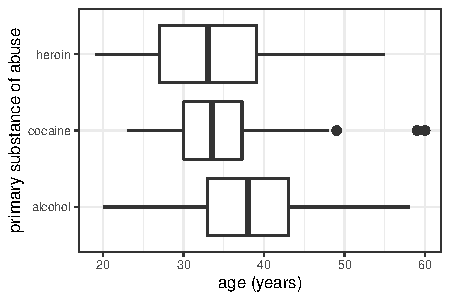
\includegraphics[width=\maxwidth]{figures/fig-bwplot2-1} 
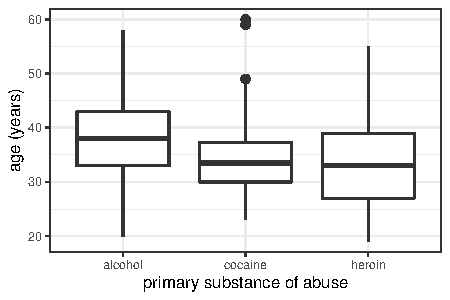
\includegraphics[width=\maxwidth]{figures/fig-bwplot2-2} 

}



\end{knitrout}

And we can combine this idea with conditioning. Careful: The quantitative variable must be the ``y" variable in the formula.

\begin{knitrout}
\definecolor{shadecolor}{rgb}{0.969, 0.969, 0.969}\color{fgcolor}\begin{kframe}
\begin{alltt}
\hlkwd{gf_boxplot}\hlstd{(age} \hlopt{~} \hlstd{substance} \hlopt{|} \hlstd{homeless,} \hlkwc{data}\hlstd{=HELPrct)}
\end{alltt}
\end{kframe}

{\centering 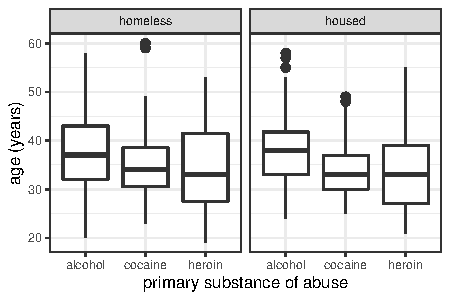
\includegraphics[width=\maxwidth]{figures/fig-bwplot3-1} 

}



\end{knitrout}

\subsection{Small data sets}
When we have relatively small data sets, it may not make sense to use a boxplot.  
With very few observations, boxplots can be misleading, in that they suggest the presence of 
more observations than are really contained in the dataset.
In these cases, it may be better to display all the data.  \function{gf_jitter()} allows you to put a categorical variable along one axis and a quantitative variable along the other.  
For some data sets, either option can produce a plot that gives a good picture
of the data.
\begin{knitrout}
\definecolor{shadecolor}{rgb}{0.969, 0.969, 0.969}\color{fgcolor}\begin{kframe}
\begin{alltt}
\hlkwd{gf_jitter}\hlstd{( weight} \hlopt{~} \hlstd{sex,} \hlkwc{data} \hlstd{= Mosquitoes,} \hlkwc{width} \hlstd{=} \hlnum{0.1}\hlstd{,} \hlkwc{height} \hlstd{=} \hlnum{0}\hlstd{)}
\hlkwd{gf_boxplot}\hlstd{( weight} \hlopt{~} \hlstd{sex,} \hlkwc{data} \hlstd{= Mosquitoes)}
\end{alltt}
\end{kframe}

{\centering 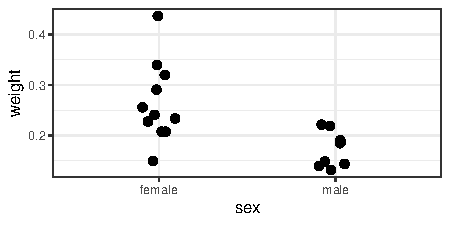
\includegraphics[width=\maxwidth]{figures/fig-xyplot-quant-by-cat-1} 
\includegraphics[width=\maxwidth]{figures/fig-xyplot-quant-by-cat-2} 

}



\end{knitrout}

Note the effect of the  \code{width = 0.1, height = 0} -- 
this tells \function{gf_jitter()} to move each data point slightly left or right, but not at all up or down. 
to reduces overplotting (data points being plotted exactly on top of one another) without losing any information,
making it clearer how many data points were observed for each possible combination of x- and y-values. 

\section{Summarizing Categorical Variables}

The most common summary of a categorical variable is the \term{proportion} 
of observations in each category. For a single category:
\begin{align*}
\hat p & = \frac{\mbox{number in one category}}{n}
\end{align*}
Proportions can be expressed as fractions, decimals or percents.  
For example, if there are 
10 observations in one category and $n = 50$ observations in all, then 
\[
\hat p = \frac{10}{25} = \frac{2}{5} =  0.40 = 40\%
\]

If we code our categorical variable using 1 for observations in a
single category of interst -- ``the one category" --
and 0 for observations in any other category, then
\emph{a proportion is a sample mean}.

\[
\frac{ 1 + 1 + 1 + 1 + 1 + 1 + 1 + 1 + 1 + 1 + 
0 + 0 + 0 + 0 + 0 + 0 + 0 + 0 + 0 + 0 + 0 + 0 + 0 + 0 + 0 }{25} = \frac{10}{25}
\]

\section{Relationships Between Two Variables}

It is also possible to give numerical summaries of the relationship
between two variables.  The most common one is the \term{correlation coefficient},
which we will learn about later.

\newpage
\section{Exercises}

\begin{problem}
	Create a data set with $n = 6$ values, each an integer between 0 and 10 (inclusive) 
	that has the smallest possible variance.  
	Compute the mean and variance of this data set ``by hand''
	(that is, without using \function{mean()} or \function{sd()} or \function{var()} 
	in \R\ or similar
	features on a calculator).
\end{problem}

\begin{solution}
	The variance will be smallest if all the values are equal to the mean value.
	In that case the variance will be 0.

	If you require all of the numbers to be distinct, the best you can do is 
	6 consecutive numbers
\begin{knitrout}
\definecolor{shadecolor}{rgb}{0.969, 0.969, 0.969}\color{fgcolor}\begin{kframe}
\begin{alltt}
\hlstd{x} \hlkwb{<-} \hlnum{1}\hlopt{:}\hlnum{6}
\hlkwd{mean}\hlstd{(}\hlopt{~}\hlstd{x)}
\end{alltt}
\begin{verbatim}
## [1] 3.5
\end{verbatim}
\begin{alltt}
\hlkwd{sd}\hlstd{(}\hlopt{~}\hlstd{x)}
\end{alltt}
\begin{verbatim}
## [1] 1.871
\end{verbatim}
\end{kframe}
\end{knitrout}
\end{solution}

\begin{problem}
	Create a data set with $n = 6$ values, each an integer between 0 and 10 (inclusive) 
	that has the largest possible variance.  
	Compute the variance of this data set ``by hand''
	(that is, without using \function{mean()} or \function{sd()} or 
	\function{var()} in \R\ or similar features on a calculator).
\end{problem}

\begin{solution}
	The variance will be smallest if all the values are far from the mean.
	If we have a data set with three 0's and 3 10's, then the mean is 5 and the 
	variance is
\begin{knitrout}
\definecolor{shadecolor}{rgb}{0.969, 0.969, 0.969}\color{fgcolor}\begin{kframe}
\begin{alltt}
\hlstd{(} \hlnum{3}\hlopt{*}\hlstd{(}\hlnum{0}\hlopt{-}\hlnum{5}\hlstd{)}\hlopt{^}\hlnum{2} \hlopt{+} \hlnum{3}\hlopt{*}\hlstd{(}\hlnum{10}\hlopt{-}\hlnum{5}\hlstd{)}\hlopt{^}\hlnum{2} \hlstd{)} \hlopt{/} \hlnum{5}
\end{alltt}
\begin{verbatim}
## [1] 30
\end{verbatim}
\end{kframe}
\end{knitrout}
	If you require the numbers to be distinct, then the best we can do is
\begin{knitrout}
\definecolor{shadecolor}{rgb}{0.969, 0.969, 0.969}\color{fgcolor}\begin{kframe}
\begin{alltt}
\hlstd{x} \hlkwb{<-} \hlkwd{c}\hlstd{(}\hlnum{0}\hlstd{,}\hlnum{1}\hlstd{,}\hlnum{2}\hlstd{,}\hlnum{8}\hlstd{,}\hlnum{9}\hlstd{,}\hlnum{10}\hlstd{)}
\hlkwd{mean}\hlstd{(}\hlopt{~}\hlstd{x)}
\end{alltt}
\begin{verbatim}
## [1] 5
\end{verbatim}
\begin{alltt}
\hlkwd{sd}\hlstd{(}\hlopt{~}\hlstd{x)}
\end{alltt}
\begin{verbatim}
## [1] 4.472
\end{verbatim}
\end{kframe}
\end{knitrout}
\end{solution}

\begin{problem}
	Create side-by-side boxplots of the variable \variable{i1} (average number of
	drinks per day) comparing the different \variable{substance} groups
	in the \dataframe{HELPrct} data frame.

	For each \variable{substance} group, explain how you can tell from the 
	boxplots whether the mean will be larger than the median or the median 
	larger than the mean.
\end{problem}

\begin{solution}
\begin{knitrout}
\definecolor{shadecolor}{rgb}{0.969, 0.969, 0.969}\color{fgcolor}\begin{kframe}
\begin{alltt}
\hlkwd{gf_boxplot}\hlstd{(i1} \hlopt{~} \hlstd{substance ,} \hlkwc{data} \hlstd{= HELPrct)}
\end{alltt}
\end{kframe}

{\centering \includegraphics[width=\maxwidth]{figures/fig-unnamed-chunk-36-1} 

}



\end{knitrout}
	The means are larger because the distributions have longer tails in the 
	higher direction.  
\end{solution}

\begin{problem}
	Compute the mean and median values of \variable{i1} (average number of
	drinks per day) for each of the \variable{substance} groups in the 
	\dataframe{HELPrct} data frame.
\end{problem}

\begin{solution}
\begin{knitrout}
\definecolor{shadecolor}{rgb}{0.969, 0.969, 0.969}\color{fgcolor}\begin{kframe}
\begin{alltt}
\hlkwd{mean}\hlstd{(i1} \hlopt{~} \hlstd{substance,} \hlkwc{data} \hlstd{= HELPrct)}
\end{alltt}
\begin{verbatim}
## alcohol cocaine  heroin 
##  29.192  12.132   8.879
\end{verbatim}
\begin{alltt}
\hlkwd{median}\hlstd{(i1} \hlopt{~} \hlstd{substance,} \hlkwc{data} \hlstd{= HELPrct)}
\end{alltt}
\begin{verbatim}
## alcohol cocaine  heroin 
##      25       6       4
\end{verbatim}
\end{kframe}
\end{knitrout}
\end{solution}

\shipoutProblems

\ifsolutions
\ifsolutionslocal
\newpage
\section*{Solutions}
\shipoutSolutions
\fi
\fi




\Chapter{Probability}

\section{Key Definitions and Ideas}

\begin{description}
\item[random process]
A repeatable process that has multiple unpredictable potential outcomes.

Although we sometimes use language that suggests that a \emph{particular result} is 
random, it is really the \emph{process} that is random, not its results.

\item[outcome]
A potential result of a random process.

\item[sample space]
The set of all possible potential outcomes of a random process.

\item[event]
A subset of the sample space.  
That is, a set of outcomes (possibly all or none of the outcomes).

Statisticians often use capital letters from the beginning of the alphabet
for events.

\item[trial] One repetition of a random process.

\item[mutually exclusive] events.
Events that cannot happen on the same trial.

\item[probability] A numerical value between 0 and 1 assigned to 
an event to indicate how often the event occurs (in the long run).

\item[random variable]
A random variable is a variable whose value is a numerical outcome of a random process.

Examples of random variables: 
\begin{itemize}
\item
Roll a die and record the number.
\item
Roll two dice and record the sum.
\item
Flip 100 coins and count the number of heads.
\item
Sample 1000 people and count how many approve of the job the president is doing.
\end{itemize}

Note: Statisticians usually use capital letters (often from the end of the alphabet)
for random variables, like this:  
Let $X$ be the number of heads in 10 flips of a fair coin.  What is $\Prob(X = 5)$?


\item[probability distribution]
The distribution of a random variable.
(Remember that a distribution describes \emph{what values?} and 
\emph{with what freqency?})
\end{description}

As an example of a probability distribution, we can first consider a \emph{discrete} random variable.  Most of the examples of random variables given above are discrete. In other words, the values they can take on come from a set containing a finite number of possible values.  For example, if you roll a 6-sided die and record the number that comes up, there are only size possible outcomes, which are equally likely: the integers 1, 2, 3, 4, 5 and 6.  For discrete random variables, the probability distribution shows all the possible values on the x-axis, and the likelihood of observing each of those values on the y-axis.  Since there are a finite number of possible values that can be observed, these likelihoods are actually the \emph{probabilities} of observing each outcome, and the sum of all the probabilities must be 1 (see section 3.3 for details).  For our example, where we rolled a die and recorded the value:

\begin{knitrout}
\definecolor{shadecolor}{rgb}{0.969, 0.969, 0.969}\color{fgcolor}

{\centering \includegraphics[width=\maxwidth]{figures/fig-discrete-pmf-1} 

}



\end{knitrout}

Things are a bit more complicated for \emph{continuous} random variables (the ones that can take on any numerical value).  Here, there sample space (the set of possible distinct values the random variable can take on) is infinite.  One consequence of this fact is that the interpretation of the y-axis values of the probability distribution changes.  The y-axis will still indicate the relative likelihood of observing any given value of the random variable.  However, here the random variable can take on an infinite number of possible values.  In this case, we can't interpret the y-axis values as probabilities.  They y axis units are called ``Likelihood" or "Density", and they indicate the relative frequency of each outcome. For a densityplot, Density is scaled such that the integral over all possible x-values (the area under the curve) is 1. (For a histogram, Density is scaled so that the total area of all the boxes added together is 1.)  We can think of the histograms and density plots we have been creating using continuous variables from R datasets as attempts to use data to approximate the distributions of random variables.  For example, we might consider the growth of flower petals of the iris \textit{Iris setosa} as a random process, and let \texttt{X} be a random variable that is the length of each iris petal.  We could plot a histogram to approximate the distribution of \texttt{X} using the variable \texttt{Petal.Length} from the \dataframe{iris} data (from the \pkg{datasets} package in base R).

\begin{knitrout}
\definecolor{shadecolor}{rgb}{0.969, 0.969, 0.969}\color{fgcolor}

{\centering \includegraphics[width=\maxwidth]{figures/fig-cont-pdf-1} 

}



\end{knitrout}

\newpage

\section{Calculating Probabilities Empirically}

We would like to calculate the probability of an event
$A$, denoted $\Prob(A)$.

In the next section, we will see how to calculate probabilities based on the Axioms of probability, and logic.  But first, we will consider ways to make the calculations empirically -- based on observing many repetitions of a random process (in real life or in a computer simulation) and observing how often an event of interest occurs.

Random processes are repeatable, so practically, we can calculate empirical probabilities by simply repeating the process
over and over and keeping track of how often the event $A$ occurs.
For example, we could flip a coin 10,000 times and see what fraction 
are heads.\footnote{This has actually been done a couple of times 
in history, including once by mathematician John Kerrich while he was a prisoner of war during World War II.}

\[
\mbox{Empirical Probability} = 
\frac{\mbox{number of times $A$ occured}}
{\mbox{number of times random process was repeated}}
\]

Modern computing provides another way to compute empirical probabilities.
If we can simulate our random process on a computer, then we can 
repeat the process many times very quickly.  

\begin{example}
\question
What is the probability of getting exactly 5 heads 
if you flip a fair coin 10 times?  Using our random variable notation, let $X$ 
be the number of heads in 10 flips of a fair coin.  We want to know $\Prob(X=5)$.

\answer 
The \function{rflip()} function simulates flipping a coin as many times as we like.
\begin{knitrout}
\definecolor{shadecolor}{rgb}{0.969, 0.969, 0.969}\color{fgcolor}\begin{kframe}
\begin{alltt}
\hlkwd{rflip}\hlstd{(}\hlnum{10}\hlstd{)}
\end{alltt}
\begin{verbatim}
## 
## Flipping 10 coins [ Prob(Heads) = 0.5 ] ...
## 
## T T H T H H T H T T
## 
## Number of Heads: 4 [Proportion Heads: 0.4]
\end{verbatim}
\end{kframe}
\end{knitrout}
The \function{do()} function allows us to execute an R command ("do" somthing in R) over and over, as many times as we choose.  Here, our \function{rflip()} command simulates 10 coin-flips.  First we'll "do" our command three times and show the results.  
Then we'll do it 10,000 times and store the results in a variable called \texttt{tosses}, so we 
can create a table and a plot showing the empirical distribution.

\begin{knitrout}
\definecolor{shadecolor}{rgb}{0.969, 0.969, 0.969}\color{fgcolor}\begin{kframe}
\begin{alltt}
\hlkwd{do}\hlstd{(}\hlnum{3}\hlstd{)} \hlopt{*} \hlkwd{rflip}\hlstd{(}\hlnum{10}\hlstd{)}
\end{alltt}
\begin{verbatim}
##    n heads tails prop
## 1 10     3     7  0.3
## 2 10     6     4  0.6
## 3 10     6     4  0.6
\end{verbatim}
\begin{alltt}
\hlkwd{do}\hlstd{(}\hlnum{10000}\hlstd{)} \hlopt{*} \hlkwd{rflip}\hlstd{(}\hlnum{10}\hlstd{)} \hlkwb{->} \hlstd{tosses}
\hlkwd{tally}\hlstd{(}\hlopt{~} \hlstd{heads,} \hlkwc{data} \hlstd{= tosses,} \hlkwc{format} \hlstd{=} \hlstr{"prop"}\hlstd{)}
\end{alltt}
\begin{verbatim}
## heads
##      0      1      2      3      4      5      6      7      8      9     10 
## 0.0003 0.0086 0.0458 0.1157 0.2044 0.2468 0.2092 0.1160 0.0423 0.0103 0.0006
\end{verbatim}
\begin{alltt}
\hlkwd{gf_histogram}\hlstd{(} \hlopt{~} \hlstd{heads,} \hlkwc{data} \hlstd{= tosses,} \hlkwc{binwidth} \hlstd{=} \hlnum{1}\hlstd{)}
\end{alltt}
\end{kframe}

{\centering \includegraphics[width=\maxwidth]{figures/fig-coin-tosses-1} 

}



\end{knitrout}


Based on this sample, we would estimate that 
$\Prob(X = 5) \approx 0.247$.
\end{example}

\begin{example}
\question Use simulations to estimate the probability of rolling doubles
using two fair standard dice.

\answer
We can simulate rolling a die with the following code:
\begin{knitrout}
\definecolor{shadecolor}{rgb}{0.969, 0.969, 0.969}\color{fgcolor}\begin{kframe}
\begin{alltt}
\hlnum{1}\hlopt{:}\hlnum{6}                \hlcom{# the numbers 1 through 6}
\end{alltt}
\begin{verbatim}
## [1] 1 2 3 4 5 6
\end{verbatim}
\begin{alltt}
\hlkwd{resample}\hlstd{(}\hlkwc{x} \hlstd{=} \hlnum{1}\hlopt{:}\hlnum{6}\hlstd{,} \hlkwc{size}\hlstd{=}\hlnum{10}\hlstd{)}  \hlcom{# ten rolls of a 6-sided die}
\end{alltt}
\begin{verbatim}
##  [1] 6 5 2 6 6 5 6 3 4 4
\end{verbatim}
\end{kframe}
\end{knitrout}
The first 2 input arguments of \function{resample()} are \texttt{x} (the set of values from which you want to resample) and \texttt{size} (the number of items to choose from \texttt{x}).  You can also think of \texttt{size} as the number of \emph{times} to sample from \texttt{x}, if you are imagining sampling one item from \texttt{x} each time.

If we do this 10,000 times for each of two dice...
\begin{knitrout}
\definecolor{shadecolor}{rgb}{0.969, 0.969, 0.969}\color{fgcolor}\begin{kframe}
\begin{alltt}
\hlstd{die1} \hlkwb{<-} \hlkwd{resample}\hlstd{(}\hlnum{1}\hlopt{:}\hlnum{6}\hlstd{,} \hlnum{10000}\hlstd{)}
\hlstd{die2} \hlkwb{<-} \hlkwd{resample}\hlstd{(}\hlnum{1}\hlopt{:}\hlnum{6}\hlstd{,} \hlnum{10000}\hlstd{)}
\hlcom{# let's check that things look reasonable}
\hlkwd{head}\hlstd{(die1)}
\end{alltt}
\begin{verbatim}
## [1] 6 1 2 4 1 5
\end{verbatim}
\begin{alltt}
\hlkwd{head}\hlstd{(die2)}
\end{alltt}
\begin{verbatim}
## [1] 5 5 3 5 6 2
\end{verbatim}
\end{kframe}
\end{knitrout}
Then we can tabulate how often the two numbers matched in one of two ways:
\begin{knitrout}
\definecolor{shadecolor}{rgb}{0.969, 0.969, 0.969}\color{fgcolor}\begin{kframe}
\begin{alltt}
\hlkwd{tally}\hlstd{(} \hlopt{~}\hlstd{(die1}\hlopt{==}\hlstd{die2) )}    \hlcom{# NOTE the double == here}
\end{alltt}
\begin{verbatim}
## (die1 == die2)
##  TRUE FALSE 
##  1712  8288
\end{verbatim}
\begin{alltt}
\hlkwd{prop}\hlstd{(} \hlopt{~}\hlstd{(die1}\hlopt{==}\hlstd{die2) )}     \hlcom{# NOTE the double == here}
\end{alltt}
\begin{verbatim}
## prop_TRUE 
##    0.1712
\end{verbatim}
\end{kframe}
\end{knitrout}
So the probability appears to be approximately 0.171.

\end{example}


\begin{example}
\question
	Use simulation to estimate the probability of rolling a sum of 8 when rolling two fair six-sided dice.

\answer
We have already generated 10000 random rolls, so let's just reuse them.  (Alternatively, we could generate new rolls.)
\begin{knitrout}
\definecolor{shadecolor}{rgb}{0.969, 0.969, 0.969}\color{fgcolor}\begin{kframe}
\begin{alltt}
\hlstd{s} \hlkwb{<-} \hlstd{die1} \hlopt{+} \hlstd{die2}
\hlcom{# R adds element-wise: }
\hlcom{#   first entry of die1 + first of die2, }
\hlcom{#   second to second, etc.}
\hlkwd{prop}\hlstd{(} \hlopt{~} \hlstd{(s} \hlopt{==} \hlnum{8}\hlstd{) )}
\end{alltt}
\begin{verbatim}
## prop_TRUE 
##    0.1387
\end{verbatim}
\end{kframe}
\end{knitrout}

We can estimate the probability of any sum the same way.
\begin{knitrout}
\definecolor{shadecolor}{rgb}{0.969, 0.969, 0.969}\color{fgcolor}\begin{kframe}
\begin{alltt}
\hlkwd{tally}\hlstd{(} \hlopt{~} \hlstd{s )}
\end{alltt}
\begin{verbatim}
## s
##    2    3    4    5    6    7    8    9   10   11   12 
##  292  536  870 1085 1397 1701 1387 1073  830  557  272
\end{verbatim}
\begin{alltt}
\hlkwd{tally}\hlstd{(} \hlopt{~} \hlstd{s,} \hlkwc{format} \hlstd{=} \hlstr{"percent"} \hlstd{)}   \hlcom{# if we are too lazy to divide by 10000 ourselves}
\end{alltt}
\begin{verbatim}
## s
##     2     3     4     5     6     7     8     9    10    11    12 
##  2.92  5.36  8.70 10.85 13.97 17.01 13.87 10.73  8.30  5.57  2.72
\end{verbatim}
\end{kframe}
\end{knitrout}

Here's a slightly fancier version that puts all the information into a data frame.  Note the use of the function \function{data.frame()} to create the data table:
\begin{knitrout}
\definecolor{shadecolor}{rgb}{0.969, 0.969, 0.969}\color{fgcolor}\begin{kframe}
\begin{alltt}
\hlstd{rolls} \hlkwb{<-} \hlkwd{data.frame}\hlstd{(} \hlkwc{first} \hlstd{= die1,} \hlkwc{second} \hlstd{= die2,} \hlkwc{sum} \hlstd{= die1} \hlopt{+} \hlstd{die2 )}
\hlkwd{head}\hlstd{(rolls)}
\end{alltt}
\begin{verbatim}
##   first second sum
## 1     6      5  11
## 2     1      5   6
## 3     2      3   5
## 4     4      5   9
## 5     1      6   7
## 6     5      2   7
\end{verbatim}
\begin{alltt}
\hlkwd{tally}\hlstd{(} \hlopt{~}\hlstd{sum,} \hlkwc{data} \hlstd{= rolls,} \hlkwc{format} \hlstd{=} \hlstr{"proportion"}\hlstd{)}
\end{alltt}
\begin{verbatim}
## sum
##      2      3      4      5      6      7      8      9     10     11     12 
## 0.0292 0.0536 0.0870 0.1085 0.1397 0.1701 0.1387 0.1073 0.0830 0.0557 0.0272
\end{verbatim}
\begin{alltt}
\hlkwd{gf_histogram}\hlstd{(} \hlopt{~} \hlstd{sum,} \hlkwc{data} \hlstd{= rolls,} \hlkwc{binwidth} \hlstd{=} \hlnum{1}\hlstd{)}    \hlcom{# setting width is important for integer data}
\end{alltt}
\end{kframe}

{\centering \includegraphics[width=\maxwidth]{figures/fig-unnamed-chunk-44-1} 

}



\end{knitrout}
\end{example}

\section{Calculating Probabilities Theoretically}

The theoretical method combines
\begin{enumerate}
\item Some basic facts about probability (the Probability Axioms and Rules),
\item Some assumptions about the particular situation at hand, and 
\item Mathematical reasoning (arithmetic, algebra, logic, etc.).
\end{enumerate}

\subsection{The Three Probability Axioms}

Let $S$ be the sample space and let $A$ and $B$ be events.
\begin{enumerate}
\item Probability is between 0 and 1: $0 \le \Prob(A) \le 1$.
\item The probability of the sample space is 1: $\Prob(S) = 1$.
\item Additivity: 
If $A$ and $B$ are mutually exclusive, then 
$\Prob(A \tor B) = \Prob(A) + \Prob(B)$.
\end{enumerate}

\subsubsection{Notation Notes}
$\Prob(A \tor B)$ is the probability that either $A$ or $B$ (or both) 
occurs.  Often this is written $\Prob(A \union B)$.  $A \union B$ is usually read
``$A$ union $B$''.  The union of two sets is the set that contains all elements of both sets.

$\Prob(A \tand B)$ is the probability that \emph{both} $A$ and $B$ occur.
This is also written $\Prob (A \intersect B)$.  $A \intersect B$ is usually read
``$A$ intersect $B$''.  

Saying that $A$ and $B$ are mutually exclusive is the same as saying that there are no
outcomes in $A\intersect B$, i.e., that $A \intersect B = \emptyset$.

\subsection{Other Probability Rules}
These rules all follow from the axioms (although we will not necessarily prove them all here).
\subsubsection*{The Addition Rule}

If events $A$  and $B$ are mutually exclusive, then 
\[
\Prob(A \tor B) = \Prob(A) + \Prob(B)
\; .
\]

More generally,
\[
\Prob(A \tor B) = \Prob(A) + \Prob(B) - \Prob(A \tand B)
\; .
\]


\subsubsection*{The Complement Rule}

\[
\Prob(\tnot A) = 1 - \Prob(A)
\]


\subsubsection*{The Equally Likely Rule}

If the sample space consists of $n$ equally likely outcomes, then
the probability of an event $A$ is given by
\[
\Prob(A) = \frac{ \mbox{number of outcomes in $A$}}{n}
=\frac{ \card{A} }{\card{S} }\; .
\]

\emph{Warning:} One of the most common mistakes in probability is to apply this rule
when the outcomes are not equally likely.

\begin{examples}
\begin{enumerate}
\item Coin Toss: $\Prob(\mbox{heads}) = \frac{1}{2}$ if heads and tails are 
equally likely.
\item Rolling a Die: $\Prob(\mbox{even}) = \frac{3}{6}$ if the die is 
fair (each of the six numbers equally likely to occur).

\newpage

\item
Sum of two Dice: the sum is a number between 2 and 12, but these numbers
are NOT equally likely.  

There are 36 equally likely combinations of two dice:

\begin{center}
\large
\begin{tabular}{|*{6}{c|}}
\hline
1,1 & 2,1 & 3,1 & 4,1 & 5,1 & 6,1 
\\ \hline
1,2 & 2,2 & 3,2 & 4,2 & 5,2 & 6,2 
\\ \hline
1,3 & 2,3 & 3,3 & 4,3 & 5,3 & 6,3 
\\ \hline
1,4 & 2,4 & 3,4 & 4,4 & 5,4 & 6,4 
\\ \hline
1,5 & 2,5 & 3,5 & 4,5 & 5,5 & 6,5 
\\ \hline
1,6 & 2,6 & 3,6 & 4,6 & 5,6 & 6,6
\\ \hline
\end{tabular}
\end{center}

Let $X$ be the sum of two dice.
\begin{itemize}
\item $\Prob(X = 3) = \frac{2}{36} = \frac{1}{18}$
\item $\Prob(X = 7) = \frac{6}{36} = \frac{1}{6}$
\item $\Prob(\mbox{doubles}) = \frac{6}{36} = \frac{1}{6}$
\end{itemize}


\item
Punnet Squares

\begin{center}
\large
\begin{tabular}{c|cc}
& A & a \\ \hline
A & AA & Aa \\ 
a & Aa & aa \\ 
\end{tabular}
\end{center}
This example comes from animal or human genetics. Here, we consider a gene with two alleles:  A is the dominant allele, and a is the recessive one.  Each individual has two copies of every gene, so there are three possible combinations of alleles (called ``genotypes"): AA, Aa, and aa. AA and Aa individuals have the dominant A physical characteristic (called the ``phenotype"); aa individuals have the recessive a phenotype. Imagine that two Aa individuals mate and produce offspring. In this Aa $\times$ Aa cross,
if A is the dominant allele, then the probability of the dominant
phenotype is $\frac{3}{4}$, and the probability of the recessive 
phenotype is $\frac{1}{4}$ because each of the four possible crossings is equally likely.

\begin{center}
	\includegraphics[width = .5\textwidth]{images/date-punnet.png}
  
  Cartoon credit: \url{http://xkcd.com/634/}
\end{center}

\end{enumerate}

\end{examples}

\newpage

\section{Conditional Probability}


\begin{example}
\label{condKids}%
\label{example:condKids}%
  \question
  Suppose a family has two children and one of them is a boy.
  What is the probability that the other is a girl?

  \answer
 % First we introduce some notation.  Let $X$ be a random variable
 % that counts the number of girls and let $Y$ be a random variable
 % that counts the number of boys (since they have Y chromosomes).
 % We'll also 
  We'll make the simplifying assumption that boys and girls are 
  equally likely (which is not exactly true).  Under that assumption,
  there are four equally likely families:  BB, BG, GB, and GG.  But only three
  of these have at least one boy, and we already know our family has at least one boy, so our sample space is really
  $\set{ BB, BG, GB}$.
  Of these, two have a girl as well as a boy.
  So the probability is $2/3$ (see Figure~\ref{fig:condKids}).  
  \authNote{moved illustration to a figure -- 2010-12-06}%

\begin{figure}[h]
	\begin{center}
	  GG \qquad \fbox{\textbf{GB} \qquad \textbf{BG} \qquad {BB}}  
	\qquad \qquad $\mbox{probability} = 2/3$
  \end{center}
\caption{Illustrating the sample space for Example~\ref{example:condKids}.}
\label{fig:condKids}%
\end{figure}

  We can also think of this in a different way.   In our original sample space
  of four equally likely families,
  \begin{align*}
	\evProb{at least one girl} & =  3/4 \; , \\ % \mbox{ , and } \\
	\evProb{at least one girl \emph{and} at least one boy} & =  2/4 \; , \tand\\
	\frac{2/4}{3/4} & =  2/3 \; ;
  \end{align*}
  so $2/3$ of the time when there is at least one boy, there is also a girl.
  We will denote this probability as 
  $\evProb{at least one girl $\mid$ at least one boy}$.
  We'll read this as ``the probability that there is at least one girl \emph{given that} 
  there is at least one boy''.  
  See Figure~\ref{fig:VennConditional} and Definition~\ref{def:condProb}.
\end{example}


\begin{figure}[h]
\begin{center}
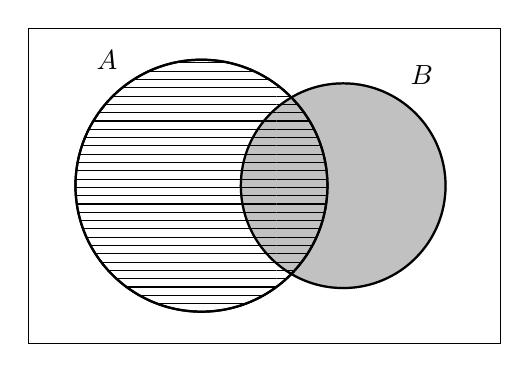
\begin{tikzpicture}
  \draw(0,0) rectangle (6,4);
  \draw(1,3.6) node{$A$};
  \draw(5,3.4) node{$B$};
  \draw[thick,fill = black!80,opacity = 0.3](4,2) circle(1.3cm);
  \draw[thick,pattern = horizontal lines](2.2,2) circle(1.6cm);
  \draw[thick](2.2,2) circle(1.6cm);
  \draw[thick](4,2) circle(1.3cm);
\end{tikzpicture}
\end{center}
\caption{A Venn diagram illustrating the definition of conditional probability.
$\Prob(A \mid B)$ is the ratio of the area of the football shaped region that is both
shaded and striped ($A \intersect B$) to the area of the shaded circle ($B$).
}
\label{fig:VennConditional}
\end{figure}

%The example above indicates how we should define conditional probability 
%generally.

%\todo{Venn Diagram}

\begin{boxedText}
%\begin{definition}[Conditional Probability]
  \label{def:condProb}%
  \myindex{conditional probability|defidx}%
  Let $A$ and $B$ be two events such that $\Prob(B) \neq 0$.  
  The \textbf{conditional probability} of $A$ given $B$ is defined by
  \[
  \Prob(A \mid B) = \frac{\Prob(A \intersect B) }{ \Prob(B) }
  \; .
  \]
  If $\Prob(B) = 0$, then $\Prob(A \mid B)$ is undefined.
%  \qed
\end{boxedText}

\begin{example}
  A class of $5$th graders was asked what color should be used for the class
  T-shirt, red or purple. 
  The table below contains a summary of the students' responses:

  \begin{center}
	\medskip
	\begin{tabular}{|l||r|r|}
	  \hline
  & \multicolumn{2}{c|}{Color}\\ 
          & Red & Purple \\ \hline \hline
	Girls & $7$    & $9$ \\ \hline
	Boys  & $10$   & $8$ \\ \hline
  \end{tabular}
  \medskip
\end{center}

  \question Suppose we randomly select a student from this class.
  Let $R$ be the event that a child prefers a red T-shirt.
  Let $B$ be the event that the child is a boy, and let $G$ be 
  the event that the child is a girl.  
  Express each of the following probabilities in words and 
  determine their values:
  \begin{multicols}{3}
  \begin{itemize}
	\item
	  $\Prob(R)$,
	\item
	  $\Prob(R \mid B)$,
	\item
	  $\Prob(B \mid R)$,
	\item
	  $\Prob(R \mid G)$,
	\item
	  $\Prob(G \mid R)$,
	\item
	  $\Prob(B \mid G)$.
  \end{itemize}
  \end{multicols}

  \answer 
  The conditional probabilities can be computed in two ways.  We can use the
  formula from the definition of conditional probability directly,
  or we can consider the condition event to be a new, smaller sample space
  and read the conditional probability from the table.
  \begin{itemize}
	\item
	  $\Prob(R) = 17/34 = 1/2$ because $17$ of the $34$ kids prefer red

	  This is the probability that a randomly selected student prefers red
	\item
	  $\displaystyle \Prob(R \mid B) = \frac{10/34}{18/34} = \frac{10}{18}$ 
	  because $10$ of the $18$ boys prefer red

	  This is the probability that a randomly selected boy prefers red
	\item
	  $\displaystyle \Prob(B \mid R)= \frac{10/34}{17/34} = \frac{10}{17}$ 
	  because $10$ of the $17$ students who prefer red are boys.

	  This is the probability that a randomly selected student who
	  prefers red is a boy.
	\item
	  $\displaystyle \Prob(R \mid G) = \frac{7/34}{16/34} = \frac{7}{16}$ 
	  because $7$ of the $16$ girls prefer red

	  This is the probability that a randomly selected girl prefers red

	\item
	  $\displaystyle \Prob(G \mid R) = \frac{7/34}{17/34} = \frac{7}{17}$ 
	  because $7$ of the $17$ kids who prefer red are girls.

	  This is the probability that a randomly selected kid who prefers red
	  is a girl.

	\item
	  $\displaystyle \Prob(B \mid G) = \frac{0}{16/34} = 0 $ because none of
	  the girls are boys.

	  This is the probability that a randomly selected girl is a boy.
%	  \qedskip
  \end{itemize}
\end{example}

One important use of conditional probability is as a tool to calculate the 
probability of an intersection.

\bigskip  %improve page break

\begin{boxedText}
  \label{lem:probOfInt}
  Let $A$ and $B$ be events with non-zero probability.  Then 
  \begin{align*}
  \Prob(A \intersect B) & =  \Prob(A) \cdot \Prob(B \mid A) \\
  	& =  \Prob(B) \cdot \Prob(A \mid B)  \;.
\end{align*}

  This follows directly from the definition of conditional probability by
  a little bit of algebra and can be generalized to more than two events.
\end{boxedText}

\begin{example}
  \question
  \myindex{dice|exampleidx}%
  If you roll two standard dice, what is the probability of doubles?
  (Doubles is when the two numbers match.)

  \answer
  Let $A$ be the event that we get a number between $1$ and $6$ on the first die.
  So $\Prob(A) = 1$.  Let $B$ be the event that the second number matches
  the first.  Then the probability of doubles is 
  $\Prob(A \intersect B) = \Prob(A) \cdot \Prob(B \mid A) = 1 \cdot \frac16 = \frac16$
  since regardless of what is rolled on the first die, $1$ of the $6$ possibilities 
  for the second die will match it.
\end{example}


\bigskip % improve page break

\begin{example}
  \myindex{cards|exampleidx}%
  \question
  A $5$-card hand is dealt from a standard $52$-card deck.
  What is the probability of getting a flush (all cards the same suit)?

  \answer
  Imagine dealing the cards in order.
  Let $A_i$ be the event that the $i$th card is the same suit as all
  previous cards.
  Then 
  \begin{eqnarray*}
\evProb{flush} & = & \Prob(A_1 
  \intersect  A_2
  \intersect  A_3
  \intersect  A_4
  \intersect  A_5) \\
  & = &  \Prob(A_1) 
  	\cdot \Prob(A_2 \mid A_1)
  	\cdot \Prob(A_3 \mid A_1 \intersect A_2)
  	\cdot \Prob(A_4 \mid A_1 \intersect A_2 \intersect A_3)
	\\ & &
  	\cdot \Prob(A_5 \mid A_1 \intersect A_2 \intersect A_3 \intersect A_4) \\
	& = & 1 \cdot \frac{12}{51} \cdot \frac{11}{50} \cdot \frac{10}{49} 
	\cdot \frac{9}{48} \; 
\end{eqnarray*}
%\otherqedskip
\end{example}

\begin{example}
\newcommand*\redheart{\Large \ensuremath{{\color{red!80!white}\heartsuit}}}
\newcommand*\blueheart{\Large \ensuremath{{\color{blue!80!black}\varheartsuit}}}
	\question
	In a bowl are 4 red Valentine hearts and 2 blue Valentine hearts.  

	If you reach in
	without looking and select two of the Valentines, let $X$ be the number of blue
	Valentines.  Fill in the following probability table.

	\begin{center}
		\begin{tabular}{|l|c|c|c|}
			\hline
			value of $X$ & \qquad 0 \ \qquad & \qquad 1 \ \qquad & \qquad 2 \ \qquad  
			\\
			\hline
			probability & & & 
			\\
			\hline
		\end{tabular}
	\end{center}

	\answer
$\Prob(X = 2) 
	= \Prob(\mbox{first is blue} \tand \mbox{second is blue})
	= \Prob(\mbox{first is blue}) \cdot \Prob( \mbox{second is blue} \mid \mbox{first is blue})
	= \frac26 \cdot \frac15 = \frac{2}{30}
$.
Similarly $\Prob(X = 0) 
	= \Prob(\mbox{first is red} \tand \mbox{second is red})
	= \Prob(\mbox{first is red}) \cdot \Prob( \mbox{second is red} \mid \mbox{first is red})
	= \frac46 \cdot \frac35 = \frac{12}{30}
$
Finally, $\Prob(X = 1) = 1 - \Prob(X = 0) - \Prob(X = 2) = 1 - \frac{14}{30} = \frac{16}{30}$

We can represent this using a \term{tree diagram} as well.

\begin{center}
	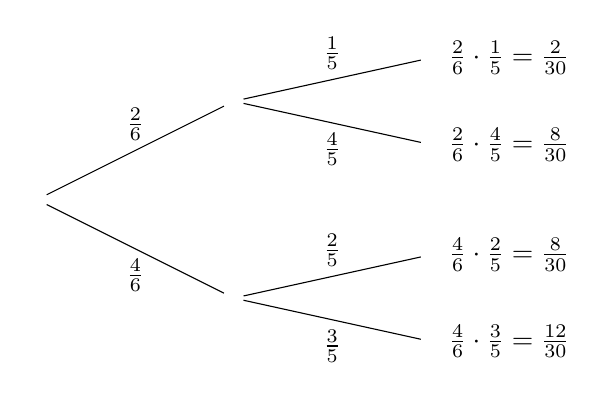
\begin{tikzpicture}
		[level 1/.style = {sibling distance = 25mm},
		 level 2/.style = {sibling distance = 11mm},
		 level distance = 25mm] 
			\node {} [grow' = right]
			child {node {\blueheart} 
				child {node (bb) {\blueheart} edge from parent node[above]{$\frac15$}} 
				child {node (br) {\redheart}  edge from parent  node[below]{$\frac45$}} 
				edge from parent node[above]{$\frac26$} 
				}
			child {node {\redheart}  
				child {node (rb) {\blueheart} edge from parent  node[above]{$\frac25$}} 
				child {node (rr) {\redheart}  edge from parent  node[below]{$\frac35$}} 
				edge from parent node[below]{$\frac46$} 
			} ; 
			\node [right of = bb] {$\frac26 \cdot \frac15 = \frac{2}{30}$};
			\node [right of = br] {$\frac26 \cdot \frac45 = \frac{8}{30}$};
			\node [right of = rb] {$\frac46 \cdot \frac25 = \frac{8}{30}$};
			\node [right of = rr] {$\frac46 \cdot \frac35 = \frac{12}{30}$};
	\end{tikzpicture}
\end{center}
The edges in the tree represent conditional probabilities which we can multiply together
to the probability that all events on a particular branch happen.  The first level of branching 
represents what kind of Valentine is selected first, the second level represents the 
second selection.
	
\end{example}

\newpage

\begin{example}
  \label{example:sensitivitySpecificity}%
  \question
  Suppose a test correctly 
%  \myindex{sensitivity|exampleidx}%
%  \myindex{specificity|exampleidx}%
  \myindex{medical testing|exampleidx}%
  identifies diseased people $99$\% of the time and correctly
  identifies healthy people $98$\% of the time.  
  Furthermore assume that in a certain population,
  one person in $1000$ has the disease.  
  If a random person is tested and the test comes back positive, 
  what is the probability that the person has the disease?

  \answer
  We begin by introducing some notation.  Let $D$ be the event that
  a person has the disease.  Let $H$ be the event that the person is
  healthy.  Let $+$ be the event that the test comes back positive (meaning 
  it indicates disease -- probably a negative from the perspective 
  of the person tested).  Let $-$ be the event that the test is negative.
	\begin{itemize}
	  \item $\Prob(D) = 0.001$, so $\Prob(H) = 0.999$.

	  \item $\Prob(+ \mid D) = 0.99$, so 
	  $\Prob(- \mid D) = 0.01$.

		$\Prob(+ \mid D)$ is called the \term{sensitivity} of the test.
		(It tells how sensitive the test is to the presence of the disease.)
	  \item 
		$\Prob(-\mid H) = 0.98$, so $\Prob(+\mid H) = 0.02$.
		\medskip

	  $\Prob(- \mid H)$ is called the \term{specificity} of the test.
		\smallskip

	  \item $\!\!\!\!\!$
	  \begin{tabular}[t]{rcl}
	  $\ds \Prob(D \mid +) $
		&$\! = \!$& $\displaystyle \frac{\Prob(D \intersect +)}{\Prob(+)}$
		\\[5mm]
		&$\; = \;$& 
		$\displaystyle \frac{\Prob(D) \cdot \Prob(+ \mid D)}{\Prob(D \intersect +) 
			+ \Prob(H \intersect +)  }$
			\\[5mm]
			& $\! = \!$ & $\displaystyle 
				\frac{0.001 \cdot 0.99}{0.001 \cdot 0.99 + 0.999 \cdot 0.02}
		            \; = \;  0.047$. 
		\end{tabular}
	  \end{itemize}
	  A tree diagram is a useful way to visualize these calculations.
\begin{center}
	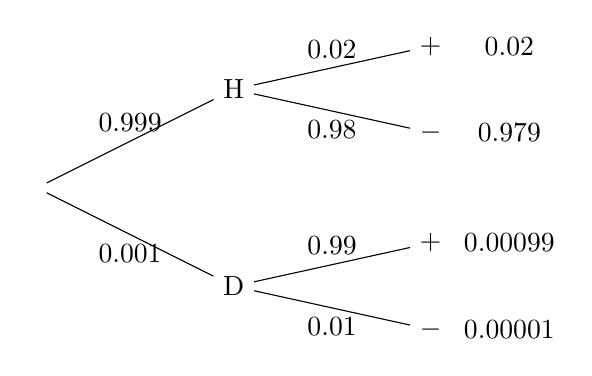
\begin{tikzpicture}
		[level 1/.style = {sibling distance = 25mm},
		 level 2/.style = {sibling distance = 11mm},
		 level distance = 25mm] 
			\node {} [grow' = right]
			child {node {H} 
				child {node (bb) {$+$} edge from parent node[above]{$0.02$}} 
				child {node (br) {$-$}  edge from parent  node[below]{$0.98$}} 
				edge from parent node[above]{$0.999$} 
				}
			child {node {D}  
				child {node (rb) {$+$} edge from parent  node[above]{$0.99$}} 
				child {node (rr) {$-$}  edge from parent  node[below]{$0.01$}} 
				edge from parent node[below]{$0.001$} 
			} ; 
			\node [right of = bb] {0.02 };
			\node [right of = br] {0.979 };
			\node [right of = rb] {0.00099 };
			\node [right of = rr] {0.00001 };
	\end{tikzpicture}
\end{center}

	  This low probability surprises most people the first time they see it.
	  This means that if the test result of a random person comes back positive,
	  the probability that that person has the disease is less than $5$\%, 
	  even though the test is ``highly accurate''.   
	  This is one reason why we do not routinely 
	  screen an entire population for a rare disease -- such screening would 
	  produce many more false positives than true positives.

	  Of course, if a doctor orders a test, it is usually because there 
	  are some other symptoms.  This changes the \emph{a priori} probability
	  that the patient has the disease.  
%	  Exercise~\ref{prob:bayesDisease}
%	  gives you a chance to explore this further.
\end{example}

\newpage

\subsection{Independence}

\begin{boxedText}
  \label{def:independentEvents}%
  \myindex{independent events|defidx}%
  Let $A$ and $B$ be two events such that $\Prob(B) = \Prob(B \mid A)$.
  Such events are called \term{independent}.
\end{boxedText}

When events are independent, then 
$\Prob(A \tand B) = \Prob(A) \cdot \Prob(B \mid A) = \Prob(A) \cdot \Prob(B)$.
This makes probability calculations much simpler -- but it only applies
for independent events.

\begin{example}
	\question 
	What is the probability of rolling double sixes with standard 6-sided dice?

	\answer
	Let $A$ be the event that the first die is a 6 and let $B$ be the event that the 
	second die is a 6.  Since $A$ and $B$ are independent, 
	$\Prob(A \tand B) = \Prob(A) \cdot \Prob(B) = \frac16 \cdot \frac16 = \frac{1}{36}$.
\end{example}

\begin{example}
	\question What is the probability of flipping a coin five times and getting 5 heads?

	\answer  Since each coin toss is independent of the others, the probability
	of getting five heads is the product of the probabilities of each coin coming up
	heads:

	\[ 
	\Prob(\mbox{5 heads in 5 flips}) = (0.5)^5 = 0.031 
	\]

	
\end{example}

\begin{example}
	\question
	A manufacturer claims that 99\% of its parts will still be functioning properly 
	two years after purchase.  If you purchase 10 of these parts, what is the probability
	that all 10 of them are still functioning properly two years later (assuming the
	manufacturer's claim is correct)?

	\answer
	Let $G_i$ be the event that part $i$ is still functioning properly after two years.
	We want to calculate 
	\[
	\Prob(G_1 \tand G_2 \tand \cdots \tand G_{10})\;.
	\]
	If we assume the lifetimes of the parts are independent, then 
	\[
	\Prob(G_1 \tand G_2 \tand \cdots \tand G_{10})
	=
	\underbrace{.99 \cdot .99 \cdot .99 \cdots .99 = .99^{10}}_{\mbox{10 of these}}
	= 0.904\;.
	\]

	The independence assumption may or may not be valid.  That depends on the manufacturing
	process.  For example, if the primary way a part goes bad is that the package 
	is dropped during shipping, then if you by a box of 10 and the first part is bad, 
	they will all be bad.  And if the box was handled carefully and never dropped, and the first part used is good, they will likely all be good.  So in
	that extreme case, the probability that all 10 are functioning properly after two years
	is 99\%.



\end{example}

\newpage
\section{Exercises}

\begin{problem}
	Amy is a 92\% free throw shooter.  If she shoots
	100 free throws after practice, what is the probability that she
	makes at least 95 of them?  Use simulation to estimate this probability.

	(You can use \function{rflip()} to simulate shooting free throws.
	The \option{prob} argument lets you set the probability.  In this case,
	you need to set it to $0.92$.  Then think of a head as a made free throw
	and a tail as a missed free throw.)
\end{problem}

\begin{solution}
\begin{knitrout}
\definecolor{shadecolor}{rgb}{0.969, 0.969, 0.969}\color{fgcolor}\begin{kframe}
\begin{alltt}
\hlkwd{set.seed}\hlstd{(}\hlnum{123}\hlstd{)}    \hlcom{# so we get the same simulated results each time we compile.}
\hlstd{sims} \hlkwb{<-} \hlkwd{do}\hlstd{(}\hlnum{1000}\hlstd{)} \hlopt{*} \hlkwd{rflip}\hlstd{(}\hlnum{100}\hlstd{,} \hlkwc{prob} \hlstd{=} \hlnum{0.92}\hlstd{)}
\hlkwd{tally}\hlstd{(} \hlopt{~} \hlstd{heads} \hlopt{>} \hlnum{95}\hlstd{,} \hlkwc{data} \hlstd{= sims)}
\end{alltt}
\begin{verbatim}
## heads > 95
##  TRUE FALSE 
##    94   906
\end{verbatim}
\end{kframe}
\end{knitrout}
So the probability that Amy makes more than 95 shots in 100 attempts is approximately
0.094
\end{solution}

\begin{problem}
	\begin{enumerate}
		\item
	Use simulation to estimate the probability of rolling a difference of 2 when rolling
	two fair six-sided dice.
\item
	Make a histogram showing the results for all of the possible differences.
	\end{enumerate}

\end{problem}

\begin{solution}
\begin{knitrout}
\definecolor{shadecolor}{rgb}{0.969, 0.969, 0.969}\color{fgcolor}\begin{kframe}
\begin{alltt}
\hlstd{d} \hlkwb{<-} \hlstd{die1} \hlopt{-} \hlstd{die2}
\hlkwd{tally}\hlstd{(} \hlopt{~} \hlstd{d )}
\end{alltt}
\begin{verbatim}
## d
##   -5   -4   -3   -2   -1    0    1    2    3    4    5 
##  305  560  829 1100 1366 1712 1337 1141  851  535  264
\end{verbatim}
\begin{alltt}
\hlkwd{prop}\hlstd{(} \hlopt{~} \hlstd{(d} \hlopt{==} \hlnum{8}\hlstd{) )}
\end{alltt}
\begin{verbatim}
## prop_TRUE 
##         0
\end{verbatim}
\begin{alltt}
\hlkwd{gf_histogram}\hlstd{(} \hlopt{~} \hlstd{d,} \hlkwc{binwidth} \hlstd{=} \hlnum{1}\hlstd{)}    \hlcom{# setting width is important for integer data}
\end{alltt}
\end{kframe}

{\centering \includegraphics[width=\maxwidth]{figures/fig-unnamed-chunk-46-1} 

}



\end{knitrout}
\end{solution}

\begin{problem}
	Use simulation to estimate the probability that when dealing 
	5 cards from a standard (well-shuffled) deck of 52 cards
	all five are diamonds.  

	You can simulate the deck of cards using the numbers 1 through 52 and consider the numbers
	1 through 13 to be the diamonds.  Instead of using \function{resample()}, which would allow
	you to get the same card more than once, we need to use \function{sample()}, which does not.
	(You can also use \function{deal()} which does the same thing.)
\begin{knitrout}
\definecolor{shadecolor}{rgb}{0.969, 0.969, 0.969}\color{fgcolor}\begin{kframe}
\begin{alltt}
\hlkwd{sample}\hlstd{(}\hlnum{1}\hlopt{:}\hlnum{52}\hlstd{,} \hlnum{5}\hlstd{)}
\end{alltt}
\begin{verbatim}
## [1] 10 38 43 25 37
\end{verbatim}
\begin{alltt}
\hlkwd{sample}\hlstd{(}\hlnum{1}\hlopt{:}\hlnum{52}\hlstd{,} \hlnum{5}\hlstd{)}
\end{alltt}
\begin{verbatim}
## [1] 19 15 36 24 31
\end{verbatim}
\begin{alltt}
\hlkwd{deal}\hlstd{(}\hlnum{1}\hlopt{:}\hlnum{52}\hlstd{,} \hlnum{5}\hlstd{)}
\end{alltt}
\begin{verbatim}
## [1] 46 43 20 29 40
\end{verbatim}
\begin{alltt}
\hlkwd{deal}\hlstd{(}\hlnum{1}\hlopt{:}\hlnum{52}\hlstd{,} \hlnum{5}\hlstd{)}
\end{alltt}
\begin{verbatim}
## [1] 17 24 10 11 37
\end{verbatim}
\end{kframe}
\end{knitrout}
	There is another way to make the calculation, using the function \function{sum}. \R\ can tell you how many cards are below 14 using \function{sum} because \R\ turns TRUE into 1
	and FALSE into 0 when you do a sum.
\begin{knitrout}
\definecolor{shadecolor}{rgb}{0.969, 0.969, 0.969}\color{fgcolor}\begin{kframe}
\begin{alltt}
\hlkwd{sum}\hlstd{(} \hlkwd{sample}\hlstd{(}\hlnum{1}\hlopt{:}\hlnum{52}\hlstd{,} \hlnum{5}\hlstd{)} \hlopt{<} \hlnum{14} \hlstd{)}
\end{alltt}
\begin{verbatim}
## [1] 2
\end{verbatim}
\begin{alltt}
\hlkwd{sum}\hlstd{(} \hlkwd{sample}\hlstd{(}\hlnum{1}\hlopt{:}\hlnum{52}\hlstd{,} \hlnum{5}\hlstd{)} \hlopt{<} \hlnum{14} \hlstd{)}
\end{alltt}
\begin{verbatim}
## [1] 0
\end{verbatim}
\begin{alltt}
\hlkwd{sum}\hlstd{(} \hlkwd{sample}\hlstd{(}\hlnum{1}\hlopt{:}\hlnum{52}\hlstd{,} \hlnum{5}\hlstd{)} \hlopt{<} \hlnum{14} \hlstd{)}
\end{alltt}
\begin{verbatim}
## [1] 1
\end{verbatim}
\end{kframe}
\end{knitrout}
	You can use \function{do()} to do this many times. (Three is \emph{not} many\! We just do a small number here 
	for illustration purposes.)
\begin{knitrout}
\definecolor{shadecolor}{rgb}{0.969, 0.969, 0.969}\color{fgcolor}\begin{kframe}
\begin{alltt}
\hlkwd{do}\hlstd{(}\hlnum{3}\hlstd{)} \hlopt{*} \hlkwd{sum}\hlstd{(} \hlkwd{sample}\hlstd{(} \hlnum{1}\hlopt{:}\hlnum{52}\hlstd{,} \hlnum{5} \hlstd{)} \hlopt{<} \hlnum{14} \hlstd{)}
\end{alltt}
\begin{verbatim}
##   sum
## 1   0
## 2   0
## 3   1
\end{verbatim}
\end{kframe}
\end{knitrout}
\end{problem}

\begin{solution}
\begin{knitrout}
\definecolor{shadecolor}{rgb}{0.969, 0.969, 0.969}\color{fgcolor}\begin{kframe}
\begin{alltt}
\hlkwd{tally}\hlstd{(} \hlopt{~} \hlstd{sum,} \hlkwd{do}\hlstd{(}\hlnum{10000}\hlstd{)} \hlopt{*} \hlkwd{sum}\hlstd{(}\hlkwd{sample}\hlstd{(}\hlnum{1}\hlopt{:}\hlnum{52}\hlstd{,} \hlnum{5}\hlstd{)} \hlopt{<} \hlnum{14}\hlstd{) )}
\end{alltt}
\begin{verbatim}
## sum
##    0    1    2    3    4    5 
## 2218 3992 2826  853  107    4
\end{verbatim}
\end{kframe}
\end{knitrout}
\end{solution}

\begin{problem}
Parts in a manufacturing plant go through two quality control checks before they
are shipped.  99\% of parts pass inspection A and 98\% parts pass inspection B.
0.5\% fail both inspections.  

What percentage of parts pass both inspections?
\end{problem}

\begin{solution}
	$\Prob(\mbox{fail at least one}) = \Prob(\mbox{fail A or fail B}) =
	\Prob(\mbox{fail A}) + \Prob(\mbox{fail B}) - \Prob(\mbox{fail both})
	= 0.01 + 0.02 - 0.05 = 0.025$.

	So $\Prob(\mbox{pass both}) = 1 - 0.025 = 0.975$.
\end{solution}

\begin{problem} 
	Let $X$ be the sum of the results of rolling two fair six-sided dice.
	\begin{enumerate}
		\item
			What is $\Prob(\mbox{$X$ is even and $X < 5$})$?
		\item
			What is $\Prob(\mbox{$X$ is even or $X < 5$})$? 
	\end{enumerate}
\end{problem}

\begin{solution}
	$\Prob(\mbox{$X$ is even and $X < 5$}) 
	= \Prob(X = 2 \tor X = 4) = 1/36 + 3/36 = 4/36 = 0.083$

$\Prob(\mbox{$X$ is even or $X < 5$}) = \Prob(\mbox{$X$ is even}) + \Prob(X = 3)
= 18/36 + 2/36 = 20/36 = 0.556$.
\end{solution}

\begin{problem}
Let $Y$ be the difference between the larger and smaller number when two fair dice 
are rolled.  (So if you roll a 2 and a 4, then the value of $Y$ is 2.)  
\begin{enumerate}
	\item 
		What is $\Prob(Y = 2)$?
	\item
		What are the other possible values of $Y$?
	\item 
		Calculate the probability for each possible value of $Y$
		and put those values in a table.
\end{enumerate}
\end{problem}

\begin{solution}
	$Y = 2$ for rolls of $(3,1)$, $(4,2)$, $(5,3)$, and $(6,4)$.  Each of these 
	can also happen in the other order, so the probability is $8/36 = 2/9 = 0.222$.

\begin{center}
	\begin{tabular}{lrrrrrr}
		\hline
		value of $Y$ & 0 & 1 & 2 & 3 & 4 & 5 \\
		\hline
		probability & 6/36 & 10/36 & 8/36 & 6/36 & 4/36 & 2/36 \\
		\hline
	\end{tabular}
\end{center}
\begin{knitrout}
\definecolor{shadecolor}{rgb}{0.969, 0.969, 0.969}\color{fgcolor}\begin{kframe}
\begin{alltt}
\hlkwd{c}\hlstd{(}\hlnum{6}\hlstd{,}\hlnum{10}\hlstd{,}\hlnum{8}\hlstd{,}\hlnum{6}\hlstd{,}\hlnum{4}\hlstd{,}\hlnum{2}\hlstd{)} \hlopt{/} \hlnum{36}
\end{alltt}
\begin{verbatim}
## [1] 0.16667 0.27778 0.22222 0.16667 0.11111 0.05556
\end{verbatim}
\end{kframe}
\end{knitrout}
\end{solution}

\begin{problem}
For the probabilities below, you may assume the that for each birth,
the probability of having a boy or a girl is $1/2$ and that each birth is
independent of other births.
\begin{enumerate}
\item
Suppose a family has three kids. 
What is the probability that at least one of the kids is a boy?
\item
Suppose a family has three kids, at least one of which is a girl.
Now what is the probability that at least one of the kids is a boy?
\item
Suppose a family has three kids, at least two of which are girls.
Now what is the probability that at least one of the kids is a boy?
\end{enumerate}
\end{problem}


\begin{problem}
	A device is assembled from two primary parts.  2\% of the first type of part
	are defective and 3\% of the other type of part are defective.  The device
	only functions properly if both parts are functioning properly.
	\begin{enumerate}
	\item
	What assumption do you need to make to calculate the probability
	that a device assembled in this way will function properly?
	Is it a reasonable assumption in this situation?  Explain.
	\item
	What is the probability that that a device assembled in this way will 
	function properly?
	\end{enumerate}
\end{problem}

\begin{solution}
	Assuming failure of each part is independent of failure of the other,
	the probability that both function properly is 
	$0.98 \cdot 0.97 = 0.951$.
	
	Alternatively, if we assume that failures are mutually exclusive, then the probability of 
	failure would be $0.02 + 0.03 = 0.05$ and the probability of proper functioning would be 
	$0.95$.
	
	The independence assumption is reasonable if, for example, the two parts are made 
	by separate manufacturing processes and the device is assembled by randomly selecting a 
	part of each type, which may or may not be a good part right from the start.  
	
	The mutually exclusive failure is probably harder to justify, since likely there will
	be some situations in which both parts fail.
\end{solution}

\begin{problem}
In the situation of Example \ref{example:sensitivitySpecificity},
how does the answer change if the baseline probability of having 
the disease is $1/10$ instead of $1/1000$? (This might be the case 
if a person is exhibiting symptoms, for example.)
\end{problem}


\begin{solution}
\begin{knitrout}
\definecolor{shadecolor}{rgb}{0.969, 0.969, 0.969}\color{fgcolor}\begin{kframe}
\begin{alltt}
\hlcom{# P(D) = 0.001}
\hlnum{0.001} \hlopt{*} \hlnum{0.99} \hlopt{/} \hlstd{(}\hlnum{0.001} \hlopt{*} \hlnum{0.99} \hlopt{+} \hlnum{0.999} \hlopt{*} \hlnum{0.02}\hlstd{)}
\end{alltt}
\begin{verbatim}
## [1] 0.04721
\end{verbatim}
\begin{alltt}
\hlcom{# P(D) = 0.10}
\hlnum{0.1} \hlopt{*} \hlnum{0.9} \hlopt{/} \hlstd{(}\hlnum{0.10} \hlopt{*} \hlnum{0.99} \hlopt{+} \hlnum{0.9} \hlopt{*} \hlnum{0.02}\hlstd{)}
\end{alltt}
\begin{verbatim}
## [1] 0.7692
\end{verbatim}
\end{kframe}
\end{knitrout}
\end{solution}

\begin{problem}
According to the CDC, ``Compared to nonsmokers, men who smoke are about 23
times more likely to develop lung cancer and women who smoke are about 13 times
more likely.''  According to the American Lung Association: 
``In 2008, 21.1 million (18.3\%) women smoked in the United States 
compared to 24.8 million (23.1\%) men.''

\begin{enumerate}
	\item
		If you learn that a person is a smoker and no nothing else 
		about the person, what is the probability that the person is a woman?
	\item
		If you learn that a woman has been diagnosed with lung cancer,
		and you know nothing else about her, what is the probability that she is a
		smoker?
	\item
		If you learn that a man has been diagnosed with lung cancer,
		and you know nothing else about him, what is the probability that he is a
		smoker?
\end{enumerate}
\end{problem}

\begin{solution}
\begin{knitrout}
\definecolor{shadecolor}{rgb}{0.969, 0.969, 0.969}\color{fgcolor}\begin{kframe}
\begin{alltt}
\hlcom{# a)}
\hlnum{21.1} \hlopt{/} \hlstd{(} \hlnum{21.1} \hlopt{+} \hlnum{24.8}\hlstd{)}
\end{alltt}
\begin{verbatim}
## [1] 0.4597
\end{verbatim}
\end{kframe}
\end{knitrout}
Part b is the most interesting (once you can do that, you can do part c the same way).
Let $W$ be the event that someone is a woman, $S$ that they are a smoker, and $C$ that they
get cancer. Let $x = \Prob( C | W \intersect S^c)$.  Then $\Prob( C | W \intersect S ) = 13x$.

\begin{align*}
	\Prob( S | W \intersect C ) 
	& = \frac{ \Prob(S \intersect W \intersect C) }{\Prob(W \intersect C)}
	\\
	& = \frac{ \Prob(S \intersect W \intersect C) }
	{\Prob(S \intersect W \intersect C) + \Prob( S^c \intersect W \intersect C)}
\end{align*}
So we just need to compute the two probabilities in the denominator.
\begin{align*}
	\Prob(S \intersect W \intersect C)
	&= \Prob(W) \cdot \Prob(S \mid W) \cdot \Prob(C \mid W \intersect S) 
	\\
	&= \Prob(W) \cdot 0.183 \cdot 13x
	\\
	\Prob(S^c \intersect W \intersect C)
	&= \Prob(W) \cdot \Prob(S^c \mid W) \cdot \Prob(C \mid W \intersect S^c) 
	\\
	&= \Prob(W) \cdot 0.817 \cdot x
\end{align*}
After factoring out $x \cdot \Prob(W)$, the arithmetic is now easy:

\begin{knitrout}
\definecolor{shadecolor}{rgb}{0.969, 0.969, 0.969}\color{fgcolor}\begin{kframe}
\begin{alltt}
\hlcom{# b) After factoring out a constant from numerator and denominator we are left with}
\hlnum{0.183} \hlopt{*} \hlnum{13} \hlopt{/} \hlstd{(} \hlnum{0.183} \hlopt{*} \hlnum{13} \hlopt{+} \hlnum{.817} \hlopt{*} \hlnum{1} \hlstd{)}
\end{alltt}
\begin{verbatim}
## [1] 0.7444
\end{verbatim}
\begin{alltt}
\hlcom{# c) After factoring out a constant from numerator and denominator we are left with}
\hlnum{0.231} \hlopt{*} \hlnum{23} \hlopt{/} \hlstd{(} \hlnum{0.231} \hlopt{*} \hlnum{23} \hlopt{+} \hlnum{.769} \hlopt{*} \hlnum{1} \hlstd{)}
\end{alltt}
\begin{verbatim}
## [1] 0.8736
\end{verbatim}
\end{kframe}
\end{knitrout}

Note: Another approach to part b is to consider the sample space to be only the women.
If you do it that way, you can avoid mentioning any probabilities involving $W$.  (In the end, 
they factor out anyway.)  Of course, you can do a similar thing for the men.
\end{solution}

\begin{problem}
A manufacturing plant has kept records that show that the number of parts produced each 
day and on the proportion of parts that are defective.

\begin{center}
\begin{tabular}{|lrrrr|}
	\hline
	& Monday & Tuesday & Wednesday & Thursday \\
	\hline
	Proportion of weekly production & 20\% & 25\% & 28\% & 27\%  
	\\
	Rate of defective parts & 2\% & 1.5\% & 1\%  & 3\% 
	\\
	\hline
\end{tabular}
\end{center}
\begin{enumerate}
	\item
		If you order a part from this company, what is the probability that it was produced
		on a Monday or a Thursday?
\item
If you order a part from this company and it is defective, 
what is the probability that it was produced on a Monday or a Thursday?
\item
	If you order a part from this company and it functions properly, 
	what is the probability that it was produced on a Monday or Thursday?
\end{enumerate}
Express your answers to 3 significant digits and avoid internal rounding.

\end{problem}

\begin{solution}
You may find a tree diagram useful here to visualize these probabilities.
\begin{knitrout}
\definecolor{shadecolor}{rgb}{0.969, 0.969, 0.969}\color{fgcolor}\begin{kframe}
\begin{alltt}
\hlcom{# part a}
\hlnum{.20} \hlopt{+} \hlnum{.27}
\end{alltt}
\begin{verbatim}
## [1] 0.47
\end{verbatim}
\begin{alltt}
\hlcom{# part b: P( Wed-Thur | defective ) = P( Wed-Thur and defective ) / P(defective)}
\hlstd{a} \hlkwb{<-} \hlnum{.20} \hlopt{*} \hlnum{.02} \hlopt{+}       \hlcom{# Monday and defective}
     \hlnum{.27} \hlopt{*} \hlnum{.03}         \hlcom{# Thursday and defective}
\hlstd{b} \hlkwb{<-} \hlnum{.25} \hlopt{*} \hlnum{.015} \hlopt{+}      \hlcom{# Tuesday and defective}
     \hlnum{.28} \hlopt{*} \hlnum{.01}         \hlcom{# Wednesday and defective }
\hlstd{a} \hlopt{/} \hlstd{(a} \hlopt{+} \hlstd{b)}
\end{alltt}
\begin{verbatim}
## [1] 0.6488
\end{verbatim}
\begin{alltt}
\hlcom{# part c: P( Wed-Thur | good ) = P( Wed-Thur and good ) / P(good)}
\hlstd{c} \hlkwb{<-} \hlnum{.20} \hlopt{*} \hlnum{.98} \hlopt{+}       \hlcom{# Monday and good}
     \hlnum{.27} \hlopt{*} \hlnum{.97}         \hlcom{# Thursday and good}
\hlstd{d} \hlkwb{<-} \hlnum{.25} \hlopt{*} \hlnum{.985} \hlopt{+}      \hlcom{# Tuesday and good}
     \hlnum{.28} \hlopt{*} \hlnum{.99}         \hlcom{# Wednesday and good }
\hlstd{c} \hlopt{/} \hlstd{(c} \hlopt{+} \hlstd{d)}
\end{alltt}
\begin{verbatim}
## [1] 0.4666
\end{verbatim}
\end{kframe}
\end{knitrout}
\end{solution}

% \begin{problem}
% %% modified from
% %% http://allendowney.blogspot.com/2011/10/my-favorite-bayess-theorem-problems.html
% %% Note: not a Bayes Theorem probelm
% John had a twin brother who died at birth.  
% What is the probability that John was an identical twin?
% 
% To answer this one, you need some background information. 
% According to a Wikipedia article on twins:  
% ``Twins are estimated to be approximately 1.9\% of the world population, 
% with monozygotic [identical] twins making up 0.15\% of the total popultion---and 8\% 
% of all twins.''
% \end{problem}

\begin{problem}
An engineer orders a shipment of 100 indentical parts.  
Before accepting the shipment, he tests three  of them.  
If the they all test good, he accepts the entire shipment.  
If any of them tests bad, he rejects the shipment.

Given the good price he has gotten on these parts, the engineer
would be satisfied if at least 95\% of the parts are good.
\begin{enumerate}
\item
Suppose that there are 5 bad parts in the shipment.  What is the probability
that the shipment is rejected (even though the engineer would actually have
been satisfied with the shipment)?
\item
Suppose that there are 10 bad parts in the shipment.  What is the probability
that the shipment is accepted (even though the engineer would not be satisfied 
with this shipment)?
\end{enumerate}
\end{problem}

\begin{solution}

\begin{enumerate}
\item The engineer will accept if all three are among the 95 good parts.
The probability of accepting is
\begin{knitrout}
\definecolor{shadecolor}{rgb}{0.969, 0.969, 0.969}\color{fgcolor}\begin{kframe}
\begin{alltt}
\hlnum{95}\hlopt{/}\hlnum{100} \hlopt{*} \hlnum{94}\hlopt{/}\hlnum{99} \hlopt{*} \hlnum{93}\hlopt{/}\hlnum{98}
\end{alltt}
\begin{verbatim}
## [1] 0.856
\end{verbatim}
\end{kframe}
\end{knitrout}
The probability of rejecting is 
\begin{knitrout}
\definecolor{shadecolor}{rgb}{0.969, 0.969, 0.969}\color{fgcolor}\begin{kframe}
\begin{alltt}
\hlnum{1} \hlopt{-} \hlnum{95}\hlopt{/}\hlnum{100} \hlopt{*} \hlnum{94}\hlopt{/}\hlnum{99} \hlopt{*} \hlnum{93}\hlopt{/}\hlnum{98}
\end{alltt}
\begin{verbatim}
## [1] 0.144
\end{verbatim}
\end{kframe}
\end{knitrout}

\item
Now we accept if all three are among the 90 good parts. 
The probability of accepting is
\begin{knitrout}
\definecolor{shadecolor}{rgb}{0.969, 0.969, 0.969}\color{fgcolor}\begin{kframe}
\begin{alltt}
\hlnum{90}\hlopt{/}\hlnum{100} \hlopt{*} \hlnum{89}\hlopt{/}\hlnum{99} \hlopt{*} \hlnum{88}\hlopt{/}\hlnum{98}
\end{alltt}
\begin{verbatim}
## [1] 0.7265
\end{verbatim}
\end{kframe}
\end{knitrout}
\end{enumerate}
We see that this is not the most effective test.  It could be improved by taking 
a larger sample, and similar arithmetic could be used to determine how well a 
new protocol works (perhaps one that takes a larger sample).
\end{solution}

\begin{problem}
%% http://allendowney.blogspot.com/2011/10/my-favorite-bayess-theorem-problems.html
The blue M\&M was introduced in 1995.  
Before then, the color mix in a bag of plain M\&Ms was 
30\% Brown, 20\% Yellow, 20\% Red, 10\% Green, 10\% Orange, 10\% Tan.  
Afterward it was 24\% Blue , 20\% Green, 16\% Orange, 14\% Yellow, 13\% Red, 
13\% Brown. 

A friend of mine has two bags of M\&Ms, and he tells me that one is from 
1994 and one from 1996.  He won't tell me which is which, but he gives me one 
M\&M from each bag.  One is yellow and one is green.  
What is the probability that the yellow M\&M came from the 1994 bag?
\end{problem}

\begin{solution}
Let's use the following notation for events related to this problem:
  \begin{itemize}
  \item $G_4 = $ green from 1994 bag
  \item $G_6 = $ green from 1996 bag
  \item $Y_4 = $ yellow from 1994 bag
  \item $Y_6 = $ yellow from 1996 bag
  \end{itemize}

Then our question becomes 
\begin{align*}
\Prob( Y_4 \tand G_6 \mid 
       (Y_4 \tand G_6) \tor (Y_6 \tand G_4) )
       & =
\frac{\Prob( Y_4 \tand G_6 ) }
     {\Prob( (Y_4 \tand G_6) \tor (Y_6 \tand G_4) )}
\\
& = \frac{\Prob( Y_4 \tand G_6 ) }
     {\Prob(Y_4 \tand G_6) + \Prob(Y_6 \tand G_4)}
\end{align*}
The individual probabilities can be worked out as
\[
\Prob(Y_4 \tand G_6) = \Prob(Y_4) \cdot \Prob(G_6 \mid Y_4)
=
.20 \cdot .20 = 0.04
\]

\[
\Prob(Y_6 \tand G_4) = \Prob(Y_6) \cdot \Prob(G_4 \mid Y_6)
=
.14 \cdot .10 = 0.014
\]

Putting this all together we get

% O: .20 Y, .10 G
% N: .14 Y, .20 G
\begin{knitrout}
\definecolor{shadecolor}{rgb}{0.969, 0.969, 0.969}\color{fgcolor}\begin{kframe}
\begin{alltt}
\hlnum{.20} \hlopt{*} \hlnum{.20} \hlopt{/} \hlstd{(}\hlnum{.20} \hlopt{*} \hlnum{.20} \hlopt{+} \hlnum{.14} \hlopt{*} \hlnum{.10}\hlstd{)}
\end{alltt}
\begin{verbatim}
## [1] 0.7407
\end{verbatim}
\end{kframe}
\end{knitrout}

A tree diagram could be used to depict these probabilities as well.
\end{solution}

\shipoutProblems

\vfill

\begin{center}
	\includegraphics[width = .4\textwidth]{images/cigarettes-cartoon}
\end{center}

\ifsolutions
\ifsolutionslocal
\newpage
\section*{Solutions}
\shipoutSolutions
\fi
\fi




\chapter{Random Variables}

\begin{description}
\item[random variable]a random process that results in a number
\end{description}

We have already seen notation for and a few examples of random variables.
In this chapter we will learn a bit more about random variables.  We will
focus our attention on two types of random variables: discrete random variables
and continuous random variables.\footnote{There are important examples 
of random variables that are neither discrete nor continuous.}

\section{Discrete Random Variables}

A discrete random variable takes on values from a discrete set of possibilities,
typically either a finite set or a subset of the integers.  Here are some examples.
\begin{enumerate}
\item If we roll a die and record the number, there are six possible values,
so the random variable is discrete.
\item
If we keep flipping a coin until we get a head and record the number of coin
tosses, then the possible values of the random variable are $1, 2, 3, \dots$
This is also a discrete random variable.
\end{enumerate}


For each of the possible values of a discrete random variable, there is some
probability of that value occuring.  So to specify a discrete random variable,
we need to specify those probabilities.  When there are only a small number 
of possible value, we can do this with a table.

\begin{center}
\begin{tabular}{lccc}
\hline
value of $X$ & 0 & 1 & 2 \\
probability & 0.2 & 0.5 & 0.3 \\
\hline
\end{tabular}
\end{center}

This is really just one way of describing a function, called the 
\textbf{probability mass function} (or pmf).  The pmf satisfies
\[
f(x) = \Prob(X = x)
\]
Sometimes instead of providing a table, we will be able to specify
the pmf using a formula.  For example, we could define a pmf $g$ by

\[ g(y) = (2 - |1-y|) / 4 \mbox{ for $y \in \{0, 1, 2\}$} \]
which is the same as specifying $g$ with the following table.

\begin{center}
\begin{tabular}{lccc}
\hline
value of $Y$ & 0 & 1 & 2 \\
probability & 0.25 & 0.5 & 0.25 \\
\hline
\end{tabular}
\end{center}

Here's one more example.  Let $W$ be a random varaible that can take on any integer
value and has pmf given by
\[
h(w) = \left(\frac{1}{2}\right)^{w+1} \mbox {for $w = 0, 1, 2, 3, \dots$}
\]
So, for example, $\Prob(W = 2) = h(2) = \left(\frac12 \right)^3 = \frac18$.

Probabilities can be obtained from the pmf by adding:


\begin{itemize}
\item
$\Prob( X > 0 ) = 0.5 + 0.3 - 0.8$
\item
$\Prob( Y > 0) = 0.5 + 0.25$
\item
$\Prob(W > 0) = \frac14 + \frac18 + \frac1{16} + \cdots = \frac12$
\item
$\Prob(W > 0) = 1 - \Prob(W = 0) = 1 - \frac{1}{2} = \frac{1}{2}$
\end{itemize}

The only restrictions on a pmf are that 
\begin{enumerate}
\item
the values must all be non-negative, and 
\item
the sum (over all possible values of the random variable) must be 1.
\end{enumerate}
That way the probabilities will behave the way probabilities should.


\begin{example}
\question
Amy is a 92\% free throw shooter.  We watch her take shots until she misses and let 
$X$ be the number of shots.  What is the pmf for $X$?

\answer
This time our table would be infinite (since there is no limit to how many consecutive
free throws Amy might make), so we won't be able to write the whole table down.
But we can work out the first few probabilities:

\begin{itemize}
\item
$f(0) = \Prob(X = 0) = 0.08$.  (She has to miss the first shot.)
\item
$f(1) = \Prob(X = 1) = (0.92)(0.08)$.  (She has to make the first and miss the second.)
\item
$f(2) = \Prob(X = 2) = (0.92)^2(0.08)$.  (She has to make the first two, then miss the third.)
\end{itemize}
At this point, we see there is a general pattern that allows us to write down an 
algebraic form for the pmf:
\[
f(x) = \Prob(X = x) = (0.92)^{x-1}(0.08)
\]
where $x$ is a positive integer.  (If $x$ is not an integer, or $x < 1$, then $f(x) = 0$, since
those values are not possible.)
\end{example}


\section{Continuous Random Variables}

\subsection{Density histograms, density plots, density functions}
\myindex{density|defidx}%
A histogram is a simple picture describing the ``density" of data. 
Histogram bars are tall in regions where there is more data -- i.e., where the data are 
more ``dense''.  
\begin{knitrout}
\definecolor{shadecolor}{rgb}{0.969, 0.969, 0.969}\color{fgcolor}\begin{kframe}
\begin{alltt}
\hlkwd{library}\hlstd{(alr4)}
\hlkwd{gf_histogram}\hlstd{(}  \hlopt{~} \hlstd{Duration,} \hlkwc{data} \hlstd{= oldfaith)}
\hlkwd{gf_dhistogram}\hlstd{(} \hlopt{~} \hlstd{Duration,} \hlkwc{data} \hlstd{= oldfaith)}
\end{alltt}
\end{kframe}

{\centering \includegraphics[width=\maxwidth]{figures/fig-histograms-count-density-1} 
\includegraphics[width=\maxwidth]{figures/fig-histograms-count-density-2} 

}



\end{knitrout}

The density scale is the same scale that is used by \function{gf_dens()} and \function{gf_density()}, 
and it is the default scale for histograms created using \function{gf_dhistogram()}.

\begin{knitrout}
\definecolor{shadecolor}{rgb}{0.969, 0.969, 0.969}\color{fgcolor}\begin{kframe}
\begin{alltt}
\hlkwd{library}\hlstd{(alr4)}
\hlkwd{gf_dhistogram}\hlstd{(} \hlopt{~} \hlstd{Duration,} \hlkwc{data} \hlstd{= oldfaith,} \hlkwc{binwidth} \hlstd{=} \hlnum{20}\hlstd{,} \hlkwc{center} \hlstd{=} \hlnum{110}\hlstd{)} \hlopt
\hlkwd{gf_dens}\hlstd{(} \hlopt{~} \hlstd{Duration,} \hlkwc{data} \hlstd{= oldfaith)}
\end{alltt}
\end{kframe}

{\centering \includegraphics[width=\maxwidth]{figures/fig-histogram-density-1} 

}



\end{knitrout}

The density scale is chosen so that the area of each rectangular bar (width times height)
is equal to the proportion of the data set represented by the rectangle. 

\begin{example}
	\question Use the histogram of Old Faithful eruption times to estimate
	the proportion of eruptions that last between 100 and 120 seconds.

	\answer
In our histogram of Old Faithful eruption durations, the bar corresponding to the 
bin from 100--120 appears to have a height of about 0.09.  That gives an area of 
0.18 and indicates that approximately 18\% of the eruptions last between 100 and 120
seconds.
\begin{knitrout}
\definecolor{shadecolor}{rgb}{0.969, 0.969, 0.969}\color{fgcolor}\begin{kframe}
\begin{alltt}
\hlkwd{tally}\hlstd{(} \hlopt{~} \hlstd{(} \hlnum{100} \hlopt{<} \hlstd{Duration} \hlopt{&} \hlstd{Duration} \hlopt{<=} \hlnum{120}\hlstd{),} \hlkwc{data} \hlstd{= oldfaith,} \hlkwc{format} \hlstd{=} \hlstr{"prop"} \hlstd{)}
\end{alltt}
\begin{verbatim}
## (100 < Duration & Duration <= 120)
##   TRUE  FALSE 
## 0.1889 0.8111
\end{verbatim}
\end{kframe}
\end{knitrout}
\end{example}

The key idea behind the density scale can be expressed as 

\begin{center}
	Probability $ = $ area
\end{center}
This association of area with probability means that
the total area of all the bars will always be equal to 1 if we use the density
scale.  

It also provides us with a way to describe a distribution with a mathematical function.


\begin{boxedText}
  \label{def:pdf}%
  \myindex{probability density function|defidx}%
  \myindex{density function|defidx}%
  \myindex{pdf|see{probability density function}}%
  Let $f$ be a function such that %: \reals \to \reals$ be a function such that
  \begin{enumerate}
	  \item $f(x) \ge 0$ for all $x$,
	  \item $\displaystyle \int_{-\infty}^{\infty} f(x) \; dx = 1$.
   \end{enumerate}
   Then $f$ is called a \textbf{density function} (or probability density function,
   abbreviated pdf) and describes a continuous random variable $X$ such that
   \[
   \Prob(a\le X \le b) = \int_a^b f(x) \; dx \;.
   \]
\end{boxedText}



\begin{example}
\label{ex:triangle}%
	Let $f$ be defined by
	\[
	f(x) = \begin{cases}  
		1 - |x| & x \in [-1,1] \\
		0 & \mbox{otherwise}\\
	\end{cases}
	\]
Show that $f$ is a density function.  Let $X$ be the associated random 
variable, and compute the following probabilities:
\begin{enumerate}
	\item
		$\Prob(X\le0)$
	\item
		$\Prob(X \le 1)$
	\item
		$\Prob(X \le \frac12)$
	\item
		$\Prob(-\frac12 X \le \frac12)$
\end{enumerate}

\answer
While we could set up integrals for these, it is easier to solve them using geometry.%
\footnote{\R\ cleverly turns TRUE and FALSE into 1 and 0 when you use them in arithmetic
expressions.  The definition of \code{f()} makes use of this conversion to simplify specifying
the cases.}
\begin{knitrout}
\definecolor{shadecolor}{rgb}{0.969, 0.969, 0.969}\color{fgcolor}\begin{kframe}
\begin{alltt}
\hlstd{f} \hlkwb{<-} \hlkwd{makeFun}\hlstd{( (}\hlnum{1} \hlopt{-} \hlkwd{abs}\hlstd{(x))} \hlopt{*} \hlstd{(}\hlkwd{abs}\hlstd{(x)} \hlopt{<=} \hlnum{1}\hlstd{)} \hlopt{~} \hlstd{x )}
\hlkwd{gf_fun}\hlstd{(} \hlkwd{f}\hlstd{(x)} \hlopt{~} \hlstd{x,} \hlkwc{xlim} \hlstd{=} \hlkwd{c}\hlstd{(}\hlopt{-}\hlnum{1.5}\hlstd{,} \hlnum{1.5}\hlstd{) )}
\end{alltt}
\end{kframe}

{\centering \includegraphics[width=\maxwidth]{figures/fig-unnamed-chunk-61-1} 

}



\end{knitrout}

The entire area under the curve can be found as the area of a triangle with base 2 and height 1.
\[
\int_{-\infty}^{\infty} f(x) \; dx 
=
\int_{-1}^1 f(x) \; dx
=
\frac 12 \cdot 2 \cdot 1 = 1
\]
This implies that $f$ is a density function.

\begin{enumerate}
	\item
$\Prob(X \le 1) 
=
\int_{-\infty}^{1} f(x) \; dx 
=
\int_{-1}^{1} f(x) \; dx = 1
$
\item
		$\Prob(X \le \frac12)
		=
\int_{-\infty}^{1/2} f(x) \; dx 
=
\int_{-1}^{1/2} f(x) \; dx = 1 - \frac12 \cdot \frac12 \cdot \frac12 = \frac78
$

\item
	$\Prob( -\frac12 \le X \le \frac 12 ) 
	=
	\int_{-1/2}^{1/2} f(x) \; dx 
	=
	1 - \frac28 = \frac34
	$
\end{enumerate}

We can also let \R\ do (numerical) integration for us.  There are two ways to do this.
The first method uses the \function{integrate()} function.
\begin{knitrout}
\definecolor{shadecolor}{rgb}{0.969, 0.969, 0.969}\color{fgcolor}\begin{kframe}
\begin{alltt}
\hlkwd{integrate}\hlstd{( f,} \hlopt{-}\hlnum{Inf}\hlstd{,} \hlnum{1} \hlstd{)}
\end{alltt}
\begin{verbatim}
## 1 with absolute error < 9.2e-05
\end{verbatim}
\begin{alltt}
\hlcom{# this will be more accurate since we aren't asking R to approximate}
\hlcom{# something that we already know is exactly 0}
\hlkwd{integrate}\hlstd{( f,} \hlopt{-}\hlnum{1}\hlstd{,} \hlnum{1}\hlstd{)}
\end{alltt}
\begin{verbatim}
## 1 with absolute error < 1.1e-14
\end{verbatim}
\begin{alltt}
\hlkwd{integrate}\hlstd{( f,} \hlopt{-}\hlnum{.5}\hlstd{,} \hlnum{.5} \hlstd{)}
\end{alltt}
\begin{verbatim}
## 0.75 with absolute error < 8.3e-15
\end{verbatim}
\begin{alltt}
\hlcom{# if you just want the value without the text saying how accurate the approximation is}
\hlcom{# here are two equivalent ways to get it}
\hlkwd{value}\hlstd{(}\hlkwd{integrate}\hlstd{( f,} \hlopt{-}\hlnum{.5}\hlstd{,} \hlnum{.5} \hlstd{))}        \hlcom{# extract the value using val()}
\end{alltt}
\begin{verbatim}
## [1] 0.75
\end{verbatim}
\begin{alltt}
\hlkwd{integrate}\hlstd{( f,} \hlopt{-}\hlnum{.5}\hlstd{,} \hlnum{.5} \hlstd{)} \hlopt \hlkwd{value}\hlstd{()}   \hlcom{# %>% is the "then" operator}
\end{alltt}
\begin{verbatim}
## [1] 0.75
\end{verbatim}
\end{kframe}
\end{knitrout}

An alternative approach uses \function{antiD()} from the \pkg{mosaic} package.
\begin{knitrout}
\definecolor{shadecolor}{rgb}{0.969, 0.969, 0.969}\color{fgcolor}\begin{kframe}
\begin{alltt}
\hlstd{F} \hlkwb{<-} \hlkwd{antiD}\hlstd{(} \hlkwd{f}\hlstd{(x)} \hlopt{~} \hlstd{x)}
\hlkwd{F}\hlstd{(}\hlnum{1}\hlstd{)} \hlopt{-} \hlkwd{F}\hlstd{(}\hlopt{-}\hlnum{1}\hlstd{)}        \hlcom{# total probability -- better be 1}
\end{alltt}
\begin{verbatim}
## [1] 1
\end{verbatim}
\begin{alltt}
\hlkwd{F}\hlstd{(}\hlnum{.5}\hlstd{)} \hlopt{-} \hlkwd{F}\hlstd{(}\hlopt{-}\hlnum{1}\hlstd{)}       \hlcom{# P( -1 <= X <= 0.5 )}
\end{alltt}
\begin{verbatim}
## [1] 0.875
\end{verbatim}
\begin{alltt}
\hlkwd{F}\hlstd{(}\hlnum{.5}\hlstd{)} \hlopt{-} \hlkwd{F}\hlstd{(}\hlopt{-}\hlnum{.5}\hlstd{)}      \hlcom{# P( -.5 <= X <= .5 )}
\end{alltt}
\begin{verbatim}
## [1] 0.75
\end{verbatim}
\end{kframe}
\end{knitrout}
\end{example}

\subsection{Kernels}
\myindex{kernel|defidx}%
The \term{kernel} of a continuous random variable is a function that is a 
constant multiple of the pdf.  The reason that these are interesting
is that any kernel can be converted into a pdf by dividing by this constant.
In particular, if 
\[ 
\int_{-\infty}^{\infty} k(x) \; dx = A \;, 
\]
then $k$ is the kernel of a random variable with pdf
\[ 
f(x) = \frac{k(x)}{A} \;.
\]

\begin{example}
\label{ex:kernel}%
	\question
	The kernel of a random variable is given by 
	\[
	k(x) = x^2 \; \boolval{ x \in [0,2] } \; .
	\]
	Determine the pdf.

	\answer First we determine the value of the integral
	\[
\int_{-\infty}^{\infty} k(x) \; dx \;. 
\]
\begin{knitrout}
\definecolor{shadecolor}{rgb}{0.969, 0.969, 0.969}\color{fgcolor}\begin{kframe}
\begin{alltt}
\hlstd{k} \hlkwb{<-} \hlkwd{makeFun}\hlstd{( x}\hlopt{^}\hlnum{2} \hlopt{*} \hlstd{(} \hlnum{0} \hlopt{<=} \hlstd{x} \hlopt{&} \hlstd{x} \hlopt{<=} \hlnum{2}\hlstd{)} \hlopt{~} \hlstd{x )}
\hlkwd{plotFun}\hlstd{(}\hlkwd{k}\hlstd{(x)} \hlopt{~} \hlstd{x,} \hlkwc{xlim} \hlstd{=} \hlkwd{c}\hlstd{(}\hlopt{-}\hlnum{1}\hlstd{,}\hlnum{3}\hlstd{))}
\hlkwd{integrate}\hlstd{( k,} \hlnum{0}\hlstd{,} \hlnum{2}\hlstd{)}
\end{alltt}
\begin{verbatim}
## 2.667 with absolute error < 3e-14
\end{verbatim}
\begin{alltt}
\hlstd{K} \hlkwb{<-} \hlkwd{antiD}\hlstd{(}\hlkwd{k}\hlstd{(x)} \hlopt{~} \hlstd{x,} \hlkwc{lower.bound} \hlstd{=} \hlnum{0}\hlstd{)}
\hlkwd{K}\hlstd{(}\hlnum{2}\hlstd{)}
\end{alltt}
\begin{verbatim}
## [1] 2.667
\end{verbatim}
\end{kframe}

{\centering \includegraphics[width=\maxwidth]{figures/fig-unnamed-chunk-64-1} 

}



\end{knitrout}
Since the total area is $8/3$, if $\frac{k(x)}{8/3}$ is the pdf.
\end{example}

\subsection{Cumulative distribution functions}

\myindex{cumulative distribution function|defidx}%
\myindex{cdf|see{cumulative distribution function}}%

% The \textbf{cumulative distribution function} (cdf) returns the probability of being
% less than or equal to some value.  We generally use a capital letter ($F$, $G$, etc.)
% to denote a cdf.
% \[
% F_X(x) = \Prob( X \le x)  \; .
% \]

% If we help \R\ choose the anti-derivative, we get a useful function called 
% the \term{cumulative distribution function}, abbreviated cdf.


\begin{boxedText}
	If $X$ is a random variable, then the \term{cumulative distribution function} (cdf) for 
	$X$, often denoted $F_X$, is the function defined by
	\[
	F_X(x)  = \Prob(X \le x)
	\]
	That is, the output of the cdf reports the probability of being below a particular value.
\end{boxedText}

For a continuous random variable, the cdf is a particular anti-derivative
of the pdf.  The derivative of the cdf is the pdf.

\begin{example}
Continuing with our previous example, if we choose -1 as our lower endpoint,
then the anti-derivative will be the cdf.
\begin{knitrout}
\definecolor{shadecolor}{rgb}{0.969, 0.969, 0.969}\color{fgcolor}\begin{kframe}
\begin{alltt}
\hlstd{f} \hlkwb{<-} \hlkwd{makeFun}\hlstd{((}\hlnum{1} \hlopt{-} \hlkwd{abs}\hlstd{(x))} \hlopt{*} \hlstd{(}\hlkwd{abs}\hlstd{(x)} \hlopt{<=} \hlnum{1}\hlstd{)} \hlopt{~} \hlstd{x)}
\hlstd{F} \hlkwb{<-} \hlkwd{antiD}\hlstd{(} \hlkwd{f}\hlstd{(x)} \hlopt{~} \hlstd{x,} \hlkwc{lower.bound} \hlstd{=} \hlopt{-}\hlnum{1}\hlstd{)}   \hlcom{# We can use -1 instead of -Inf here.}
\hlkwd{F}\hlstd{(}\hlopt{-}\hlnum{1}\hlstd{)}               \hlcom{# this should be 0 since we chose -1 as the lower bound.}
\end{alltt}
\begin{verbatim}
## [1] 0
\end{verbatim}
\begin{alltt}
\hlkwd{F}\hlstd{(}\hlnum{1}\hlstd{)}                \hlcom{# P(X <= 1); should be 1}
\end{alltt}
\begin{verbatim}
## [1] 1
\end{verbatim}
\begin{alltt}
\hlkwd{F}\hlstd{(}\hlnum{.5}\hlstd{)}               \hlcom{# P(X <= 0.5)}
\end{alltt}
\begin{verbatim}
## [1] 0.875
\end{verbatim}
\begin{alltt}
\hlkwd{F}\hlstd{(}\hlnum{.5}\hlstd{)} \hlopt{-} \hlkwd{F}\hlstd{(}\hlopt{-}\hlnum{.5}\hlstd{)}      \hlcom{# P( -0.5 <= X <= 0.5 )}
\end{alltt}
\begin{verbatim}
## [1] 0.75
\end{verbatim}
\end{kframe}
\end{knitrout}
\end{example}

%\section{Working with Probability Density Funcitons}

We have already seen that we can use a pdf $f$ to calculate probabilities via integration, 
and that there is a special anti-derivative of $f$ called the cdf such that the cdf $F$
satisfies
\[
F(x) = \Prob(X \le x)
\]
This function can also be used to compute probabilities, since
\[
\Prob(a \le X \le b) = \int_a^b f(x) \; dx = F(b) - F(a)
\]
Indeed, once we learn how to get the cdf function in \R\ this will 
be our primary way to calculate probabilities in applications.

\section{Mean and Variance}
\subsection{The mean of a random variable}

The definition for the mean of a random variable will be motivated 
by the calculation of a mean of some data.

\begin{example}
	\question
  Suppose a student has taken $10$ courses
  and received $5$ A's, $4$ B's, and $1$ C.  Using the traditional numerical scale where 
  an A is worth $4$, a B is worth $3$, and a C is worth $2$, what is this student's 
  GPA (grade point average)?

  \answer
  The first thing to notice is that $\frac{4 + 3 + 2}{3} = 3$ is \emph{not} correct.
  We cannot simply add up the values and divide by the number of values.  Clearly
  this student should have a GPA that is higher than $3.0$, since there were more A's than
  C's.

  Consider now a correct way to do this calculation:
  \begin{align*}
	\mbox{GPA} &= \frac{4 + 4 + 4 + 4 + 4 + 3 + 3 + 3 + 3 + 2}{10}
	\\[2mm]
	& = \frac{5\cdot 4 + 4\cdot 3 + 1 \cdot 2}{10} \\[1mm]
	& = \frac{5}{10} \cdot 4 + \frac{4}{10}\cdot 3 + \frac{1}{10} \cdot 2 \\
	& = 4 \cdot \frac{5}{10} + 3 \cdot \frac{4}{10} + 2 \cdot \frac{1}{10} \\
	& =  3.4 \;.
\end{align*}
\end{example}
The key idea here is that the mean is a \textbf{sum of values times probabilities}.  
\[
\mbox{mean} = \sum \mbox{value} \cdot \mbox{probability}
\]
For a discrete random variable this translates to
\[
\E(X) = \sum x f(x)
\]
where the sum is taken over all possible values of $X$.

The mean of a random variable also goes by another name: \textbf{expected value}.  We 
can denote the mean of $X$ by either $\mu_X$ or $\E(X)$.

\begin{example}
Let $X$ be discrete random variable with probablilities given in the table 
below.

\begin{center}
\begin{tabular}{lccc}
\hline
value of $X$ & 0 & 1 & 2 \\
probability & 0.2 & 0.5 & 0.3 \\
\hline
\end{tabular}
\end{center}

\question What is the mean (expected value) of $X$?

\answer
$E(X) = 0 \cdot 0.2 + 1 \cdot 0.5 + 2 \cdot 0.3 = 0.5 + 0.6 = 1.1$
This value reflects the fact that the random variable is larger than
1 a bit more often than it is less than 1.
\end{example}



\begin{example}
\label{ex:raffle}%
\label{ex:raffle2}%
  A local charity is holding a raffle.  They are selling $1000$ raffle tickets 
  for \$$5$ each.  The owners of five of the raffle tickets will win a prize.  The 
  five prizes are valued at \$$25$, \$$50$, \$$100$, \$$1000$, and \$$2000$.  Let $X$ 
  be the value of the prize associated with a random raffle ticket ($0$ for 
  non-winning tickets). 
  Then:
  \begin{itemize}
	\item $\evProb{the ticket wins a prize} = \Prob(X > 0) = 5/1000$.
	\item $\evProb{the ticket wins the grand prize} = \Prob(X = 2000) = 1/1000$.
	\item $\evProb{the ticket wins a prize worth more than \$$75$} 
	  	= \Prob(X > 75) = 3/1000$.
  \end{itemize}
  
  The expected value of a ticket is
  
\[
  0 \cdot \frac{995}{1000} 
  + 25 \cdot \frac{1}{1000}
  + 50 \cdot \frac{1}{1000}
  + 100 \cdot \frac{1}{1000}
  + 1000 \cdot \frac{1}{1000}
  + 2000 \cdot \frac{1}{1000}
\]
\begin{knitrout}
\definecolor{shadecolor}{rgb}{0.969, 0.969, 0.969}\color{fgcolor}\begin{kframe}
\begin{alltt}
\hlnum{25} \hlopt{*} \hlnum{.001} \hlopt{+} \hlnum{50} \hlopt{*} \hlnum{0.001} \hlopt{+} \hlnum{100} \hlopt{*} \hlnum{0.001} \hlopt{+} \hlnum{1000} \hlopt{*} \hlnum{0.001} \hlopt{+} \hlnum{2000} \hlopt{*} \hlnum{0.001}
\end{alltt}
\begin{verbatim}
## [1] 3.175
\end{verbatim}
\begin{alltt}
\hlcom{# R can help us set up this sum:}
\hlkwd{sum}\hlstd{(}\hlkwd{c}\hlstd{(}\hlnum{25}\hlstd{,} \hlnum{50}\hlstd{,} \hlnum{100}\hlstd{,} \hlnum{1000}\hlstd{,} \hlnum{2000}\hlstd{)} \hlopt{*} \hlnum{0.001}\hlstd{)}
\end{alltt}
\begin{verbatim}
## [1] 3.175
\end{verbatim}
\end{kframe}
\end{knitrout}
%%% \qedskip
\end{example}


When working with a continuous random variable, 
we replace the sum with an integral and replace the 
probabilities with our density function to get the following definition:

\[
\E(X) = \mu_X = \int_{-\infty}^{\infty} x f(x) \; dx
\]

If you recall doing center of mass problems you may recognize this integral as 
the first moment.
(For pdfs, we don't need to divide by the ``mass'' because the total ``mass'' is the area under the curve, which will always be 1 for a random variable).

Note: It is possible that the integral used to define the mean will fail to converge.
In that case, we say that the random variable has no mean or that the mean fails to exist.%
\footnote{Actually, we will require that $\int_{\infty}^{\infty} |x| f(x) \; dx$ converges.  
If this integral fails to converge, we will also say that the distribution has no mean.}

\begin{example}
	\question Compute the mean of our triangle distribution from Example~\ref{ex:triangle}.

	\answer We simply compute the integral from the definition.

	\begin{align*}
	\E(X) & = \int_{-1}^{1} x f(x) \; dx 
	\\
	& = \int_{-1}^{0} x (x-1) \; dx + \int_{0}^1 x ( 1-x ) \; dx 
	\\
	& = \int_{-1}^{0} x^2-x) \; dx + \int_{0}^1 x-x^2 ) \; dx  
	\\
	& = \left.\frac{x^3}{3} - \frac{x^2}{2} \right|_{-1}^0
	+ \left. \frac{x^2}{2} - \frac{x^3}{3} \right|_{0}^1
	\\
	& = \frac13 - \frac12 + \frac12 - \frac13 = 0
	\end{align*}

	This isn't surprising, by symmetry we would expect this result.

	We could also calculate this numerically in \R:
\begin{knitrout}
\definecolor{shadecolor}{rgb}{0.969, 0.969, 0.969}\color{fgcolor}\begin{kframe}
\begin{alltt}
\hlstd{f} \hlkwb{<-} \hlkwd{makeFun}\hlstd{( (}\hlnum{1} \hlopt{-} \hlkwd{abs}\hlstd{(x))} \hlopt{*} \hlstd{(}\hlkwd{abs}\hlstd{(x)} \hlopt{<=} \hlnum{1}\hlstd{)} \hlopt{~} \hlstd{x)}
\hlstd{xf} \hlkwb{<-} \hlkwd{makeFun}\hlstd{( x} \hlopt{*} \hlkwd{f}\hlstd{(x)} \hlopt{~} \hlstd{x )}
\hlkwd{integrate}\hlstd{(xf,} \hlopt{-}\hlnum{1}\hlstd{,} \hlnum{1}\hlstd{)}
\end{alltt}
\begin{verbatim}
## 0 with absolute error < 3.7e-15
\end{verbatim}
\begin{alltt}
\hlstd{F} \hlkwb{<-} \hlkwd{antiD}\hlstd{( x} \hlopt{*} \hlkwd{f}\hlstd{(x)} \hlopt{~} \hlstd{x,} \hlkwc{lower.bound} \hlstd{=} \hlopt{-}\hlnum{1}\hlstd{)}
\hlkwd{F}\hlstd{(}\hlopt{-}\hlnum{1}\hlstd{)}  \hlcom{# should be 0}
\end{alltt}
\begin{verbatim}
## [1] 0
\end{verbatim}
\begin{alltt}
\hlkwd{F}\hlstd{(}\hlnum{1}\hlstd{)}
\end{alltt}
\begin{verbatim}
## [1] 0
\end{verbatim}
\end{kframe}
\end{knitrout}
\end{example}

\subsection{Variance}

Arguing similarly, we can compute the variance of a discrete or continuous random
variable using 
\begin{itemize}
\item discrete:
\(
\Var(X) = \sigma^2_X = \sum_x (x-\mu_X)^2 f(x) \; dx  
\)
\item
continuous:
\(
\Var(X) = \sigma^2_X = \int_{-\infty}^{\infty} (x-\mu_X)^2 f(x) \; dx
\)
\end{itemize}
These can be combined into a single definition by writing
\[
\Var(X) = \E((X - \mu_X)^2) \;.
\]

Note: It is possible that the sum or integral used to define the mean (or the variance) will fail 
to converge. In that case, we say that the random variable has no mean (or variance) or that the 
mean (or variance)  fails to exist.%
\footnote{Actually, we will require that 
$\int_{\infty}^{\infty} |x| f(x) \; dx$ converges and   
$\int_{\infty}^{\infty} |x|^2 f(x) \; dx$ converges.  
If these integrals (or the corresponding sums for discrete random variables) fail to converge, 
we will say that the distribution has no mean (or variance).}

\begin{example}
	\question Compute the variance of the triangle random variable
	from the Example~\ref{ex:triangle}.
	
\answer
\begin{knitrout}
\definecolor{shadecolor}{rgb}{0.969, 0.969, 0.969}\color{fgcolor}\begin{kframe}
\begin{alltt}
\hlstd{f} \hlkwb{<-} \hlkwd{makeFun}\hlstd{( (}\hlnum{1} \hlopt{-} \hlkwd{abs}\hlstd{(x))} \hlopt{*} \hlstd{(}\hlkwd{abs}\hlstd{(x)} \hlopt{<=} \hlnum{1}\hlstd{)} \hlopt{~} \hlstd{x)}
\hlstd{xxf} \hlkwb{<-} \hlkwd{makeFun}\hlstd{( (x}\hlopt{-}\hlnum{0}\hlstd{)}\hlopt{^}\hlnum{2} \hlopt{*} \hlkwd{f}\hlstd{(x)} \hlopt{~} \hlstd{x )}
\hlkwd{integrate}\hlstd{(xxf,} \hlopt{-}\hlnum{1}\hlstd{,} \hlnum{1}\hlstd{)}
\end{alltt}
\begin{verbatim}
## 0.1667 with absolute error < 1.9e-15
\end{verbatim}
\begin{alltt}
\hlstd{G} \hlkwb{<-} \hlkwd{antiD}\hlstd{( (x}\hlopt{-}\hlnum{0}\hlstd{)}\hlopt{^}\hlnum{2} \hlopt{*} \hlkwd{f}\hlstd{(x)} \hlopt{~} \hlstd{x)}
\hlkwd{G}\hlstd{(}\hlnum{1}\hlstd{)} \hlopt{-} \hlkwd{G}\hlstd{(}\hlopt{-}\hlnum{1}\hlstd{)}
\end{alltt}
\begin{verbatim}
## [1] 0.1667
\end{verbatim}
\end{kframe}
\end{knitrout}
\end{example}

Some simple algebraic manipulations of the sum or integral above shows that
\begin{align}
\Var(X) &= \E(X^2) - \E(X)^2
\label{eqn:varshortcut}
\end{align}

\begin{problem} 
Let $f(x) = 5/4 - x^3$  on $[0,1]$.  

\begin{enumerate}
	\item
		Show that $f$ is a pdf.
	\item
			Calculate $\Prob(X \le \frac12)$.
	\item
			Calculate $\Prob(X \ge \frac12)$.
	\item
			Calculate $\Prob(X = \frac12)$.
\end{enumerate}

\end{problem}

\begin{solution}
\begin{knitrout}
\definecolor{shadecolor}{rgb}{0.969, 0.969, 0.969}\color{fgcolor}\begin{kframe}
\begin{alltt}
\hlstd{f} \hlkwb{<-} \hlkwd{makeFun}\hlstd{( (}\hlnum{5}\hlopt{/}\hlnum{4} \hlopt{-} \hlstd{x}\hlopt{^}\hlnum{3}\hlstd{)} \hlopt{*} \hlstd{(} \hlkwd{abs}\hlstd{(x}\hlopt{-}\hlnum{.5}\hlstd{)} \hlopt{<=} \hlnum{.5} \hlstd{)} \hlopt{~} \hlstd{x )}
\hlkwd{plotFun}\hlstd{(}\hlkwd{f}\hlstd{(x)} \hlopt{~} \hlstd{x,} \hlkwc{x.lim} \hlstd{=} \hlkwd{c}\hlstd{(}\hlopt{-}\hlnum{1}\hlstd{,}\hlnum{2}\hlstd{))}  \hlcom{# quick plot to make sure things look correct.}
\hlstd{F} \hlkwb{<-} \hlkwd{antiD}\hlstd{(}\hlkwd{f}\hlstd{(x)} \hlopt{~}\hlstd{x)}
\hlcom{# part a:  f(x) >=0, so we just need to check that the total area is 1}
\hlkwd{F}\hlstd{(}\hlnum{1}\hlstd{)} \hlopt{-} \hlkwd{F}\hlstd{(}\hlnum{0}\hlstd{)} \hlopt{==} \hlnum{1}
\end{alltt}
\begin{verbatim}
## [1] TRUE
\end{verbatim}
\begin{alltt}
\hlkwd{F}\hlstd{(}\hlnum{1}\hlopt{/}\hlnum{2}\hlstd{)} \hlopt{-} \hlkwd{F}\hlstd{(}\hlnum{0}\hlstd{)}     \hlcom{# part b}
\end{alltt}
\begin{verbatim}
## [1] 0.6094
\end{verbatim}
\begin{alltt}
\hlkwd{F}\hlstd{(}\hlnum{1}\hlstd{)} \hlopt{-} \hlkwd{F}\hlstd{(}\hlnum{1}\hlopt{/}\hlnum{2}\hlstd{)}     \hlcom{# part c}
\end{alltt}
\begin{verbatim}
## [1] 0.3906
\end{verbatim}
\begin{alltt}
\hlkwd{F}\hlstd{(}\hlnum{1}\hlopt{/}\hlnum{2}\hlstd{)} \hlopt{-} \hlkwd{F}\hlstd{(}\hlnum{1}\hlopt{/}\hlnum{2}\hlstd{)}   \hlcom{# part d}
\end{alltt}
\begin{verbatim}
## [1] 0
\end{verbatim}
\end{kframe}

{\centering \includegraphics[width=\maxwidth]{figures/fig-unnamed-chunk-69-1} 

}



\end{knitrout}
\end{solution}



\begin{example}
	\question Compute the mean and variance of the random variable with pdf given by
	
	\[ g(x) = \frac{3x^2}{8} \boolval{x \in [0,2]} \;. \]
	This is the pdf computed in Example~\ref{ex:kernel}.
	
\answer
\begin{knitrout}
\definecolor{shadecolor}{rgb}{0.969, 0.969, 0.969}\color{fgcolor}\begin{kframe}
\begin{alltt}
\hlstd{g} \hlkwb{<-} \hlkwd{makeFun}\hlstd{( (}\hlnum{3} \hlopt{*} \hlstd{x}\hlopt{^}\hlnum{2}\hlopt{/}\hlnum{8} \hlstd{)} \hlopt{*} \hlstd{(}\hlnum{0} \hlopt{<=} \hlstd{x} \hlopt{&} \hlstd{x} \hlopt{<=} \hlnum{2}\hlstd{)} \hlopt{~} \hlstd{x )}
\hlstd{m} \hlkwb{<-} \hlkwd{antiD}\hlstd{( x} \hlopt{*} \hlkwd{g}\hlstd{(x)} \hlopt{~} \hlstd{x,} \hlkwc{lower.bound} \hlstd{=} \hlnum{0}\hlstd{)(}\hlnum{2}\hlstd{)}  \hlcom{# all in one step instead of defining F or G}
\hlstd{m}
\end{alltt}
\begin{verbatim}
## [1] 1.5
\end{verbatim}
\begin{alltt}
\hlstd{v} \hlkwb{<-} \hlkwd{antiD}\hlstd{( (x} \hlopt{-} \hlstd{m)}\hlopt{^}\hlnum{2} \hlopt{*} \hlkwd{g}\hlstd{(x)} \hlopt{~} \hlstd{x,} \hlkwc{m} \hlstd{= m,} \hlkwc{lower.bound} \hlstd{=} \hlnum{0}\hlstd{)(}\hlnum{2}\hlstd{)}
\hlstd{v}
\end{alltt}
\begin{verbatim}
## [1] 0.15
\end{verbatim}
\begin{alltt}
\hlcom{# here's the alternate computation}
\hlkwd{antiD}\hlstd{( x}\hlopt{^}\hlnum{2} \hlopt{*} \hlkwd{g}\hlstd{(x)} \hlopt{~} \hlstd{x,} \hlkwc{lower.bound} \hlstd{=} \hlnum{0}\hlstd{)(}\hlnum{2}\hlstd{)} \hlopt{-} \hlstd{m}\hlopt{^}\hlnum{2}
\end{alltt}
\begin{verbatim}
## [1] 0.15
\end{verbatim}
\end{kframe}
\end{knitrout}
\end{example}

As with data, the standard deviation is the square root of the variance.

\subsection{Quantiles}

Quantiles solve equations of the form
\[
\int_{-\infty}^x f(t) \; dt = F(x) = \Prob(X \le x) = q
\]
where $q$ is known and $x$ is unknown.  So the 50th percentile (which is the 0.5-quantile
or the median) is the number such that 
\[
\Prob(X \le x) = 0.5 \;.
\]

\begin{example}
	\question What is the 25th percentile of the triangle distribution in
	Example~\ref{ex:triangle}?

	\answer
	We need to solve for $x$ in the following equation:
	\[
	0.25 = \Prob( X \le x)  \; .
	\]
	We can do this by working out the integral involved:
	\begin{align*}
	0.25 &= \int_{-1}^{x} 1 - |t| \; dt 
	\\
	 &= \int_{-1}^{x} 1 + t \; dt 
	 \\
	 &=  \left. t + t^2/2 \right|_{-1}^{x}
	 \\
	 &=   x + x^2/2 + 1 - 1^2/2  
	 \\
	 &=  x + x^2/2 + 1/2
	 \\
	 0 & =  x^2/2 + x + 1/4
	 \\
	 0 & =  2x^2 + 4x + 1
\end{align*}
So by the quadratic formula, $x = \frac12 \sqrt{2} - 1 = -0.293$.

We can check this by evaluating the cdf.
\begin{knitrout}
\definecolor{shadecolor}{rgb}{0.969, 0.969, 0.969}\color{fgcolor}\begin{kframe}
\begin{alltt}
\hlstd{x} \hlkwb{<-} \hlnum{1}\hlopt{/}\hlnum{2}\hlopt{*}\hlkwd{sqrt}\hlstd{(}\hlnum{2}\hlstd{)} \hlopt{-} \hlnum{1}
\hlkwd{F}\hlstd{(x)}
\end{alltt}
\begin{verbatim}
## [1] 0
\end{verbatim}
\end{kframe}
\end{knitrout}

This could also be done geometrically by solving $\frac12 y^2 = \frac14$ and letting
$x = -1 + y$.
\end{example}


\section{Some Important Families of Distributions}

\myindex{parameter}%
For now, we will consider only distributions of continuous random variables (probability density functions).  We will leave set aside discrete random variables (probability mass function) until quite a bit later in the course.

A family of distributions is a collection of distributions that share some
common features.  Typically, these are described by giving a pdf that has
one or more \term{parameters}. A parameter is simply a number that describes
(a feature of) a distribution that distinguishes between members of the family.
In this section we describe briefly
some of the important distributions and how to work with them in \R.

\subsection{Triangle Distributions}
\myindex{triangle distribution|defidx}%
\myindex{triangular distribution|see{triangle distribution}}%
The example distribution in the previous section is usually referred to as a 
triangle distribution (or triangular distribution)
because of the shape of its pdf.  There are, of course,
many triangle distributions.  A triangle distribution is specified with three
numbers: $a$, the minimum; $b$, the maximum, and $c$, the location of the peak.
A triangle distribution is symmetric if the peak is halfway between the minimum
and maximum ($c = \frac{a+b}{2}$).

When $X$ is a random variable with a triangle distribution, we will write
$X \sim \Tri(a,b,c)$.  For many of the most common
distributions, \R\ has several functions that facilitate computation with
those distributions.  The triangle distributions are not in the base \R\ 
distribution, but they can be added by requiring the \pkg{triangle} package.

For each distribution, there are four functions in \R\ that always start
with a single letter followed by a name for the distribution.  In the case 
of the triangle distributions, these functions are 

\begin{center}
\begin{tabular}{ll}
	\hline
	Function & What it does \\
	\hline
	\texttt{dtriangle(x,a,b,c)} & Computes value of the pdf at \texttt{x}
	\\
	\texttt{ptriangle(q,a,b,c)}     & Computes value of the cdf at \texttt{x}, i.e., 
	$\Prob(X \le \texttt{q})$
	\\
	\texttt{qtriangle(p,a,b,c)}     & Computes quantiles, that is a value $q$ so that 
	$\Prob(X \le \texttt{q}) = \texttt{p}$
    \\
	\texttt{rtriangle(n,a,b,c)} & Randomly samples \texttt{n} values from the 
	$\Tri(\texttt{a},\texttt{b},\texttt{c})$ distribution
	\\
	\hline
\end{tabular}
\end{center}


\begin{example}
\label{ex:triangleInR}%
	\question Let $X \sim \Tri(0,4,1)$.  Use \R\ to answer the following questions.
	\begin{enumerate}
		\item Plot the pdf for $X$.
		\item What is $\Prob(X \le 1)$?
		\item What is $\Prob(X \le 2)$?
		\item What is the median of $X$?
		\item What is the mean of $X$?
	\end{enumerate}
	
\answer
The \function{gf_dist} function in the \pkg{ggformula} package allows us to 
graph the pdf for any function \R\ knows how to work with in the standard way.
For example, here is a plot of the pdf of a $\Tri(0, 4, 1)$-distribution.
\begin{knitrout}
\definecolor{shadecolor}{rgb}{0.969, 0.969, 0.969}\color{fgcolor}\begin{kframe}
\begin{alltt}
\hlkwd{library}\hlstd{(triangle)}      \hlcom{# a package that knows about triangle distributions}
\end{alltt}


{\ttfamily\noindent\bfseries\color{errorcolor}{\#\# Error in library(triangle): there is no package called 'triangle'}}\begin{alltt}
\hlkwd{gf_dist}\hlstd{(}\hlstr{"triangle"}\hlstd{,} \hlkwc{a} \hlstd{=} \hlnum{0}\hlstd{,} \hlkwc{b} \hlstd{=} \hlnum{4}\hlstd{,} \hlkwc{c} \hlstd{=} \hlnum{1}\hlstd{)}
\end{alltt}


{\ttfamily\noindent\bfseries\color{errorcolor}{\#\# Error in get(fun, mode = "{}function"{}, envir = envir): object 'dtriangle' of mode 'function' was not found}}\end{kframe}
\end{knitrout}
Here is the \R\ code to answer the remaining questions.
\begin{knitrout}
\definecolor{shadecolor}{rgb}{0.969, 0.969, 0.969}\color{fgcolor}\begin{kframe}
\begin{alltt}
\hlkwd{ptriangle}\hlstd{(}\hlnum{1}\hlstd{,} \hlnum{0}\hlstd{,} \hlnum{4}\hlstd{,} \hlnum{1}\hlstd{)}   \hlcom{# P(X <= 4); notice that his is NOT 1/2}
\end{alltt}


{\ttfamily\noindent\bfseries\color{errorcolor}{\#\# Error in ptriangle(1, 0, 4, 1): could not find function "{}ptriangle"{}}}\begin{alltt}
\hlkwd{ptriangle}\hlstd{(}\hlnum{2}\hlstd{,} \hlnum{0}\hlstd{,} \hlnum{4}\hlstd{,} \hlnum{1}\hlstd{)}   \hlcom{# P(X <= 4); also NOT 1/2}
\end{alltt}


{\ttfamily\noindent\bfseries\color{errorcolor}{\#\# Error in ptriangle(2, 0, 4, 1): could not find function "{}ptriangle"{}}}\begin{alltt}
\hlkwd{qtriangle}\hlstd{(}\hlnum{0.5}\hlstd{,} \hlnum{0}\hlstd{,} \hlnum{4}\hlstd{,} \hlnum{1}\hlstd{)} \hlcom{# median is the 0.5-quantile}
\end{alltt}


{\ttfamily\noindent\bfseries\color{errorcolor}{\#\# Error in qtriangle(0.5, 0, 4, 1): could not find function "{}qtriangle"{}}}\begin{alltt}
\hlstd{T} \hlkwb{<-} \hlkwd{antiD}\hlstd{( x} \hlopt{*} \hlkwd{dtriangle}\hlstd{(x,} \hlnum{0}\hlstd{,}\hlnum{4}\hlstd{,}\hlnum{1}\hlstd{)} \hlopt{~} \hlstd{x,} \hlkwc{lower.bound} \hlstd{=} \hlnum{0}\hlstd{)}
\hlkwd{T}\hlstd{(}\hlnum{4}\hlstd{)}                    \hlcom{# mean of X}
\end{alltt}


{\ttfamily\noindent\bfseries\color{errorcolor}{\#\# Error in dtriangle(x, 0, 4, 1): could not find function "{}dtriangle"{}}}\begin{alltt}
\hlkwd{integrate}\hlstd{(} \hlkwd{makeFun}\hlstd{( x} \hlopt{*} \hlkwd{dtriangle}\hlstd{(x,} \hlnum{0}\hlstd{,}\hlnum{4}\hlstd{,}\hlnum{1}\hlstd{)} \hlopt{~} \hlstd{x) ,} \hlnum{0}\hlstd{,} \hlnum{4}\hlstd{)}
\end{alltt}


{\ttfamily\noindent\bfseries\color{errorcolor}{\#\# Error in dtriangle(x, 0, 4, 1): could not find function "{}dtriangle"{}}}\end{kframe}
\end{knitrout}
\end{example}



\begin{problem}
	Repeat parts (2) -- (4) of Example~\ref{ex:triangleInR} using geometry 
	rather than \R.

\end{problem}

\begin{solution}
	\begin{itemize}
		\item
			$\Prob(X \le 1) = \frac 12 \cdot 1 \cdot \frac12 = \frac 14$
		\item
			$\Prob(X \le 2) = 1 - \Prob(X \ge 2) =  1 - \frac12 \cdot 2 \cdot \frac13 
			= 1 - \frac 13 = \frac23$.
		\item
			The median $m$ is a number between 1 and 2 and satisfies
			$\frac 12 = \Prob(X \ge m) = \frac12 (4-m) \frac{4-m}{6}$.  
			Solving for $m$ we get $m = 4 - \sqrt{6} = 1.551$.
	\end{itemize}
\end{solution}

\begin{problem}
	Let $\displaystyle k(x) = (1 - x^2) \cdot \boolval{ x \in [-1,1] } = 
	\begin{cases}
		1-x^2 & x \in [-1,1] \\ 
		0 & \mbox{otherwise} 
	\end{cases}$ be the kernel of a continuous distribution.
	\begin{enumerate}
		\item
			Determine the pdf for this distribution.
		\item
			Compute the mean and variance for this distribution
	\end{enumerate}
\end{problem}

\begin{solution}
	The integrals are easy enough to do by hand, but here is the \R\ code 
	to compute them.
\begin{knitrout}
\definecolor{shadecolor}{rgb}{0.969, 0.969, 0.969}\color{fgcolor}\begin{kframe}
\begin{alltt}
\hlstd{k} \hlkwb{<-} \hlkwd{makeFun}\hlstd{(} \hlnum{1} \hlopt{-} \hlstd{x}\hlopt{^}\hlnum{2} \hlopt{~} \hlstd{x )}
\hlstd{K} \hlkwb{<-} \hlkwd{antiD}\hlstd{(} \hlkwd{k}\hlstd{(x)} \hlopt{~} \hlstd{x )}
\hlstd{area} \hlkwb{<-} \hlkwd{K}\hlstd{(}\hlnum{1}\hlstd{)} \hlopt{-} \hlkwd{K}\hlstd{(}\hlopt{-}\hlnum{1}\hlstd{); area}
\end{alltt}
\begin{verbatim}
## [1] 1.333
\end{verbatim}
\begin{alltt}
\hlstd{f} \hlkwb{<-} \hlkwd{makeFun}\hlstd{( (}\hlnum{1} \hlopt{-} \hlstd{x}\hlopt{^}\hlnum{2}\hlstd{)}\hlopt{/}\hlstd{A} \hlopt{~} \hlstd{x,} \hlkwc{A} \hlstd{= area )}
\hlstd{F} \hlkwb{<-} \hlkwd{antiD}\hlstd{(}\hlkwd{f}\hlstd{(x)} \hlopt{~} \hlstd{x)}
\hlkwd{F}\hlstd{(}\hlnum{1}\hlstd{)} \hlopt{-} \hlkwd{F}\hlstd{(}\hlopt{-}\hlnum{1}\hlstd{)}    \hlcom{# this should be 1 if we have done things right}
\end{alltt}
\begin{verbatim}
## [1] 1
\end{verbatim}
\begin{alltt}
\hlstd{G} \hlkwb{<-} \hlkwd{antiD}\hlstd{( x} \hlopt{*} \hlkwd{f}\hlstd{(x)} \hlopt{~} \hlstd{x )}
\hlstd{H} \hlkwb{<-} \hlkwd{antiD}\hlstd{( x}\hlopt{^}\hlnum{2} \hlopt{*} \hlkwd{f}\hlstd{(x)} \hlopt{~} \hlstd{x )}
\hlstd{m} \hlkwb{<-} \hlkwd{G}\hlstd{(}\hlnum{1}\hlstd{)} \hlopt{-} \hlkwd{G}\hlstd{(}\hlopt{-}\hlnum{1}\hlstd{); m}               \hlcom{# E(X)}
\end{alltt}
\begin{verbatim}
## [1] 0
\end{verbatim}
\begin{alltt}
\hlkwd{H}\hlstd{(}\hlnum{1}\hlstd{)} \hlopt{-} \hlkwd{H}\hlstd{(}\hlopt{-}\hlnum{1}\hlstd{)}                       \hlcom{# E(X^2)}
\end{alltt}
\begin{verbatim}
## [1] 0.2
\end{verbatim}
\begin{alltt}
\hlkwd{H}\hlstd{(}\hlnum{1}\hlstd{)} \hlopt{-} \hlkwd{H}\hlstd{(}\hlopt{-}\hlnum{1}\hlstd{)} \hlopt{-} \hlstd{m}\hlopt{^}\hlnum{2}                 \hlcom{# Var(X)}
\end{alltt}
\begin{verbatim}
## [1] 0.2
\end{verbatim}
\end{kframe}
\end{knitrout}
\end{solution}

\begin{problem}
	Let $Y \sim \Tri(0,10,4)$.  Compute $\E(Y)$ and the median of $Y$.
\end{problem}
\begin{solution}
\begin{knitrout}
\definecolor{shadecolor}{rgb}{0.969, 0.969, 0.969}\color{fgcolor}\begin{kframe}
\begin{alltt}
\hlcom{# mean:}
\hlstd{m} \hlkwb{<-} \hlkwd{antiD}\hlstd{( x} \hlopt{*} \hlkwd{dtriangle}\hlstd{(x,}\hlnum{0}\hlstd{,}\hlnum{10}\hlstd{,}\hlnum{4}\hlstd{)} \hlopt{~} \hlstd{x,} \hlkwc{lower.bound} \hlstd{=} \hlnum{0}\hlstd{)(}\hlnum{10}\hlstd{)}
\end{alltt}


{\ttfamily\noindent\bfseries\color{errorcolor}{\#\# Error in dtriangle(x, 0, 10, 4): could not find function "{}dtriangle"{}}}\begin{alltt}
\hlstd{m}
\end{alltt}
\begin{verbatim}
## [1] 0
\end{verbatim}
\begin{alltt}
\hlcom{# variance:}
\hlkwd{antiD}\hlstd{( x}\hlopt{^}\hlnum{2} \hlopt{*} \hlkwd{dtriangle}\hlstd{(x,}\hlnum{0}\hlstd{,}\hlnum{10}\hlstd{,}\hlnum{4}\hlstd{)} \hlopt{~} \hlstd{x,} \hlkwc{lower.bound} \hlstd{=} \hlnum{0}\hlstd{)(}\hlnum{10}\hlstd{)} \hlopt{-} \hlstd{m}\hlopt{^}\hlnum{2}
\end{alltt}


{\ttfamily\noindent\bfseries\color{errorcolor}{\#\# Error in dtriangle(x, 0, 10, 4): could not find function "{}dtriangle"{}}}\begin{alltt}
\hlcom{# median}
\hlkwd{qtriangle}\hlstd{(} \hlnum{0.5}\hlstd{,} \hlnum{0}\hlstd{,} \hlnum{10}\hlstd{,} \hlnum{4} \hlstd{)}
\end{alltt}


{\ttfamily\noindent\bfseries\color{errorcolor}{\#\# Error in qtriangle(0.5, 0, 10, 4): could not find function "{}qtriangle"{}}}\end{kframe}
\end{knitrout}
\end{solution}

\subsection{Uniform Distributions}
\myindex{uniform distribution|defidx}%

A uniform distribution is a described by a constant function over some interval.  Its 
shape is a rectangle.  This makes it particularly easy to calculate probabilities 
for a uniform distribution.  Despite its simplicity, the family of uniform distributions
has many applications.

We will let $X \sim \Unif(a,b)$ denote that $X$ is a uniform random variable on 
the interval from $a$ to $b$. 
In \R\, the parameters $a$ and $b$ are given more meaningful names: \code{min} and \code{max}.
We can use the following code to graph the $\Unif(1,4)$ distribution.

\begin{knitrout}
\definecolor{shadecolor}{rgb}{0.969, 0.969, 0.969}\color{fgcolor}\begin{kframe}
\begin{alltt}
\hlkwd{gf_dist}\hlstd{(}\hlstr{"unif"}\hlstd{,} \hlkwc{min} \hlstd{=} \hlnum{1}\hlstd{,} \hlkwc{max} \hlstd{=} \hlnum{4}\hlstd{,} \hlkwc{xlim} \hlstd{=} \hlkwd{c}\hlstd{(}\hlopt{-}\hlnum{1}\hlstd{,} \hlnum{6}\hlstd{))}
\end{alltt}
\end{kframe}

{\centering \includegraphics[width=\maxwidth]{figures/fig-unnamed-chunk-76-1} 

}



\end{knitrout}
Notice that the width of the non-zero portion of the pdf is 3, so the height must be $1/3$.

Probabilities involving uniform distributions are easily calculated using simple geometry,
but \R\ also provides several functions for working with uniform probability distributions.

\begin{center}
\begin{tabular}{ll}
	\hline
	Function & What it does \\
	\hline
	\texttt{dunif(x,min,max)} & Computes value of the pdf at \texttt{x}
	\\
	\texttt{punif(x,min,max)} & Computes value of the cdf at \texttt{x}, i.e., 
	$\Prob(X \le \texttt{x})$
	\\
	\texttt{qunif(p,min,max)} & Computes quantiles, that is a value of $x$ so that 
								$\Prob(X \le x) = \texttt{q}$
    \\
	\texttt{runif(n,min,max)} & Randomly samples \texttt{n} values from the 
								$\Unif(\texttt{min}, \texttt{max})$ distribution
	\\
	\hline
\end{tabular}
\end{center}

Notice the pattern to these names.  They start with the same letters as 
the functions for the triangle distributions, but replace \texttt{triangle}
with \texttt{unif}.  \emph{There are similar functions for all of the distributions
in this chapter.}

\begin{example}
	\question
	Let $X \sim \Unif(1,4)$.  Use \R\ to calculate the following values and 
	check the values using geometry:
	\begin{enumerate}
		\item $\Prob(X \le 2)$
		\item the 80th percentile of the distribution
	\end{enumerate}

	\answer
\begin{knitrout}
\definecolor{shadecolor}{rgb}{0.969, 0.969, 0.969}\color{fgcolor}\begin{kframe}
\begin{alltt}
\hlkwd{punif}\hlstd{(}\hlnum{2}\hlstd{,}\hlnum{1}\hlstd{,}\hlnum{4}\hlstd{)}   \hlcom{# P(X <= 2 )}
\end{alltt}
\begin{verbatim}
## [1] 0.3333
\end{verbatim}
\begin{alltt}
\hlstd{(}\hlnum{2}\hlopt{-}\hlnum{1}\hlstd{)} \hlopt{*} \hlnum{1}\hlopt{/}\hlnum{3}    \hlcom{# P(X <= 2 ) using area}
\end{alltt}
\begin{verbatim}
## [1] 0.3333
\end{verbatim}
\begin{alltt}
\hlkwd{qunif}\hlstd{(}\hlnum{.8}\hlstd{,} \hlnum{1}\hlstd{,}\hlnum{4}\hlstd{)} \hlcom{# 80th percentile}
\end{alltt}
\begin{verbatim}
## [1] 3.4
\end{verbatim}
\end{kframe}
\end{knitrout}
We could also get the 80th percentile by solving the equation $\frac13 (x-1) = 0.8$
From this we get $\frac{x}{3} = 0.8 + 1/3$, so $x = 3 ( 0.8 + 1/3) = 2.4 + 1 = 3.4$.
\end{example}

\begin{problem}
	Let $W \sim \Unif(0,10)$.  Compute $\E(W)$ and $\Var(W)$.
\end{problem}

\begin{solution}
\begin{knitrout}
\definecolor{shadecolor}{rgb}{0.969, 0.969, 0.969}\color{fgcolor}\begin{kframe}
\begin{alltt}
\hlcom{# mean:}
\hlstd{m} \hlkwb{<-} \hlkwd{antiD}\hlstd{( x} \hlopt{*} \hlkwd{dunif}\hlstd{(x,}\hlnum{0}\hlstd{,}\hlnum{10}\hlstd{)} \hlopt{~} \hlstd{x,} \hlkwc{lower.bound} \hlstd{=} \hlnum{0}\hlstd{)(}\hlnum{10}\hlstd{)}
\hlstd{m}
\end{alltt}
\begin{verbatim}
## [1] 5
\end{verbatim}
\begin{alltt}
\hlcom{# variance:}
\hlkwd{antiD}\hlstd{( x}\hlopt{^}\hlnum{2} \hlopt{*} \hlkwd{dunif}\hlstd{(x,}\hlnum{0}\hlstd{,}\hlnum{10}\hlstd{)} \hlopt{~} \hlstd{x,} \hlkwc{lower.bound} \hlstd{=} \hlnum{0}\hlstd{)(}\hlnum{10}\hlstd{)} \hlopt{-} \hlstd{m}\hlopt{^}\hlnum{2}
\end{alltt}
\begin{verbatim}
## [1] 8.333
\end{verbatim}
\end{kframe}
\end{knitrout}
\end{solution}


\subsection{Exponential Distributions}
\myindex{exponential distribution|defidx}%

The exponential distributions are useful for modeling the time until some ``event'' 
occurs.  The model is based on the assumptions that 
\begin{enumerate}
	\item
		The probability of an event occurring in any small interval of time 
		is proportional to the length of the time interval.  The constant
		of proportionality is the rate parameter, usually denoted by $\lambda$.
	\item
		The probabilities of events occurring in two small non-overlapping intervals
		are independent.
\end{enumerate}

\begin{examples}
	Here are some situations that might be well modeled by an exponential distribution:
	\begin{enumerate}
\item
	The time until the next radioactive decay event is detected on a Geiger counter 

\item
	The time until a space satellite is struck by a meteor (or some other space junk) 
	and disabled.

	The model would be good if (over some time span of interest) the chances of getting
	struck are always the same.  It would not be such a good model if the satellite moves
	through time periods of relatively higher and then relatively lower chances of being
	struck (perhaps because we pass through regions of more or less space debris at 
	different times of the year.)

\item
	The lifetime of some manufactured device.

	This is a pretty simple model (we'll learn better ones later) and most often is \emph{too} simple to describe the interesting features of the lifetime of a device.  In this model, failure is due to some external thing ``happening to" the device; the 
	device itself does not wear (or improve) over time.
	\end{enumerate}
\end{examples}

We will let $X \sim \Exp(\lambda)$ denote that $X$ has an exponential distribution
with rate parameter $\lambda$.   
The kernel of such a distribution is 
\[
k(x; \lambda) = e^{-\lambda x} \; \boolval{x \ge 0}
\]
Notice that the function describing this distribution is defined only for x-values that are real numbers greater than or equal to zero (in mathematical notation, the interval $[0, \infty)$.) This interval is sometimes called the ``support" of the distribution.  When using probability distributions to model data, it's important to think about whether the support of the distribution matches well with the range of possible values observed in the data.

The exponential distribution function is a pretty easy function to integrate, but \R\ provides the now familiar
functions to make things even easier.

\begin{center}
\begin{tabular}{ll}
	\hline
	Function & What it does \\
	\hline
	\texttt{dexp(x,rate)} & Computes value of the pdf at \texttt{x}
	\\
	\texttt{pexp(q,rate)}     & Computes value of the cdf at \texttt{x}, i.e., 
	$\Prob(X \le \texttt{q})$
	\\
	\texttt{qexp(p,rate)}     & Computes quantiles, that is a value $q$ so that 
	$\Prob(X \le \texttt{q}) = \texttt{p}$
    \\
	\texttt{rexp(n,rate)} & Randomly samples \texttt{n} values from the 
	$\Exp(\lambda)$ distribution
	\\
	\hline
\end{tabular}
\end{center}

\iffalse
\begin{boxedText}
	We will write $X \sim \Exp(\lambda)$ to indicate that the random variable $X$ has 
	an exponential distribution with rate parameter $\lambda$.
	\begin{center}
		\begin{tabular}{lll}
			\hline 
			parameter & $\lambda$ & \texttt{rate}
			\\
			kernel & $e^{-\lambda x}$
			\\
			pdf & $f(x; \lambda) = \lambda e^{-\lambda x} \boolval{x\ge 0}$ 
			& \texttt{dexp(x,rate)}
			\\
%			mean & $\frac{1}{\lambda}$
%			\\
%			variance & $\frac{1}{\lambda^2}$
%			\\ 
%			\hline
		\end{tabular}
	\end{center}
\end{boxedText}
\fi


\begin{knitrout}
\definecolor{shadecolor}{rgb}{0.969, 0.969, 0.969}\color{fgcolor}\begin{kframe}
\begin{alltt}
\hlkwd{gf_dist}\hlstd{(}\hlstr{"exp"}\hlstd{,} \hlkwc{rate} \hlstd{=} \hlnum{4}\hlstd{)}
\end{alltt}
\end{kframe}

{\centering \includegraphics[width=\maxwidth]{figures/fig-gf-dist-eponential-1} 

}



\end{knitrout}

\begin{problem}
	\begin{enumerate}
		\item Let $X \sim \Exp(4)$.  Use \R\ to compute $\E(X)$.
		\item Let $X \sim \Exp(10)$.  Use \R\ to compute $\E(X)$.
		\item Let $X \sim \Exp(1/5)$.  Use \R\ to compute $\E(X)$.
		\item What pattern do you notice.  Explain in terms of 
			the definition of the exponential distribution why this
			makes sense.
	\end{enumerate}
\end{problem}

\begin{solution}
\begin{knitrout}
\definecolor{shadecolor}{rgb}{0.969, 0.969, 0.969}\color{fgcolor}\begin{kframe}
\begin{alltt}
\hlkwd{antiD}\hlstd{( x} \hlopt{*} \hlkwd{dexp}\hlstd{(x,} \hlnum{4}\hlstd{)} \hlopt{~} \hlstd{x,} \hlkwc{lower.bound} \hlstd{=} \hlnum{0}\hlstd{)(}\hlnum{Inf}\hlstd{)}
\end{alltt}
\begin{verbatim}
## [1] 0.25
\end{verbatim}
\begin{alltt}
\hlkwd{antiD}\hlstd{( x} \hlopt{*} \hlkwd{dexp}\hlstd{(x,} \hlnum{10}\hlstd{)} \hlopt{~} \hlstd{x,} \hlkwc{lower.bound} \hlstd{=} \hlnum{0}\hlstd{)(}\hlnum{Inf}\hlstd{)}
\end{alltt}
\begin{verbatim}
## [1] 0.1
\end{verbatim}
\begin{alltt}
\hlkwd{antiD}\hlstd{( x} \hlopt{*} \hlkwd{dexp}\hlstd{(x,} \hlnum{1}\hlopt{/}\hlnum{5}\hlstd{)} \hlopt{~} \hlstd{x,} \hlkwc{lower.bound} \hlstd{=} \hlnum{0}\hlstd{)(}\hlnum{Inf}\hlstd{)}
\end{alltt}
\begin{verbatim}
## [1] 5
\end{verbatim}
\end{kframe}
\end{knitrout}
	It appears that the mean of an $\Exp(\lambda)$-distribution is $1/\lambda$.  This
	makes sense.  If events have at a rate of $30$ per hour, we would expect to wait
	$1/30$ of an hour (on average) for the first event to happen.
\end{solution}


%\newpage
\subsection{Gamma and Weibull Distributions}
\myindex{Gamma distribution|defidx}%
\myindex{Weibull distribution|defidx}%

The Gamma and Weibull familities of distributions are generalizations of the exponential
distribution.  Each family has two parameters, a rate parameter as in 
the exponential distribution, and an additional parameter called the shape 
parameter (denoted by $\alpha$ below).  The reciprocal of the rate parameter
is called the scale parameter.  For the Gamma distribution, \R\ lets us use
either rate or scale (and the default is rate).  For the Weibull, we must use the 
scale.

\begin{center}
	\begin{tabular}{ll}
		\hline
		distribution & kernel
		\\
		\hline
		$\Gamm(\alpha, \lambda)$ & $ k(x) = x^{\alpha-1} e^{-\lambda x} \; \boolval{x \ge 0}$
		\\
		$\Weibull(\alpha, \lambda)$ & $ k(x) = x^{\alpha-1} e^{-\lambda x^{\alpha}} \; \boolval{x \ge 0}$
		\\
		\hline
	\end{tabular}
\end{center}
Both families of distributions are supported on the interval $[0, \infty)$.)
For the most part, we won't use these formulas in calculations, 
preferring to let \R\ do the work for us. However, notice that each
of these distributions has a pdf that allows for relatively simple integration.  For the 
Gamma distributions, we need to use integration by parts ($\alpha - 1$ times).  For 
the Weibull distributions we can use a substitution: $u = x^{\alpha}$.
In each case, when $\alpha = 1$ we get an exponential distribution.

The now familiar functions are available for each of these distributions.
\begin{center}
\begin{tabular}{ll}
	\hline
	Function & What it does \\
	\hline
	\texttt{dgamma(x, shape, rate, scale = 1/rate)} & Computes value of the pdf at \texttt{x}
	\\
	\texttt{pgamma(q, shape, rate, scale = 1/rate)} 
		& Computes value of the cdf at \texttt{x}, i.e., 
	$\Prob(X \le \texttt{q})$
	\\
	\texttt{qgamma(p, shape, rate, scale = 1/rate)} 
		& Computes quantiles, that is a value $q$ so that 
	$\Prob(X \le \texttt{q}) = \texttt{p}$
    \\
	\texttt{rgamma(n, shape, rate, scale = 1/rate)} & Randomly samples \texttt{n} values from a
	Gamma distribution.
	\\
	\hline
	\texttt{dweibull(x, shape, scale = 1/rate)} & Computes value of the pdf at \texttt{x}
	\\
	\texttt{pweibull(q, shape, scale)} 
		& Computes value of the cdf at \texttt{x}, i.e., 
	$\Prob(X \le \texttt{q})$
	\\
	\texttt{qweibull(p, shape, scale)} 
		& Computes quantiles, that is a value $q$ so that 
	$\Prob(X \le \texttt{q}) = \texttt{p}$
    \\
	\texttt{rweibull(n,shape,scale)} & Randomly samples \texttt{n} values from a
	Weibull distribution.
	\\
	\hline
\end{tabular}
\end{center}

Like the exponential distributions, these distributions are skewed and only take 
on positive values.  
These distributions arise in many applications, including as more general models 
for lifetime.  As the pictures below indicate, the shape and scale parameters
are aptly named.

\begin{knitrout}
\definecolor{shadecolor}{rgb}{0.969, 0.969, 0.969}\color{fgcolor}\begin{kframe}
\begin{alltt}
\hlkwd{gf_dist}\hlstd{(}\hlstr{"gamma"}\hlstd{,} \hlkwc{params} \hlstd{=} \hlkwd{list}\hlstd{(}\hlkwc{shape} \hlstd{=} \hlnum{2}\hlstd{,} \hlkwc{rate} \hlstd{=} \hlnum{1}\hlstd{),} \hlkwc{title} \hlstd{=} \hlstr{"Gamma(2,1)"}\hlstd{)}
\hlkwd{gf_dist}\hlstd{(}\hlstr{"gamma"}\hlstd{,} \hlkwc{params} \hlstd{=} \hlkwd{list}\hlstd{(}\hlkwc{shape} \hlstd{=} \hlnum{5}\hlstd{,} \hlkwc{rate} \hlstd{=} \hlnum{1}\hlstd{),} \hlkwc{title} \hlstd{=} \hlstr{"Gamma(5,1)"}\hlstd{)}
\hlkwd{gf_dist}\hlstd{(}\hlstr{"gamma"}\hlstd{,} \hlkwc{params} \hlstd{=} \hlkwd{list}\hlstd{(}\hlkwc{shape} \hlstd{=} \hlnum{2}\hlstd{,} \hlkwc{scale} \hlstd{=} \hlnum{10}\hlstd{),} \hlkwc{title} \hlstd{=} \hlstr{"Gamma(5,10)"}\hlstd{)}
\hlkwd{gf_dist}\hlstd{(}\hlstr{"gamma"}\hlstd{,} \hlkwc{params} \hlstd{=} \hlkwd{list}\hlstd{(}\hlkwc{shape} \hlstd{=} \hlnum{5}\hlstd{,} \hlkwc{scale} \hlstd{=} \hlnum{10}\hlstd{),} \hlkwc{title} \hlstd{=} \hlstr{"Gamma(5,10)"}\hlstd{)}
\end{alltt}
\end{kframe}

{\centering \includegraphics[width=\maxwidth]{figures/fig-unnamed-chunk-80-1} 
\includegraphics[width=\maxwidth]{figures/fig-unnamed-chunk-80-2} 
\includegraphics[width=\maxwidth]{figures/fig-unnamed-chunk-80-3} 
\includegraphics[width=\maxwidth]{figures/fig-unnamed-chunk-80-4} 

}



\end{knitrout}

\begin{knitrout}
\definecolor{shadecolor}{rgb}{0.969, 0.969, 0.969}\color{fgcolor}\begin{kframe}
\begin{alltt}
\hlkwd{gf_dist}\hlstd{(}\hlstr{"weibull"}\hlstd{,} \hlkwc{params} \hlstd{=} \hlkwd{list}\hlstd{(}\hlkwc{shape} \hlstd{=} \hlnum{2}\hlstd{,} \hlkwc{scale} \hlstd{=} \hlnum{1}\hlstd{),}\hlkwc{title} \hlstd{=} \hlstr{"Weibull(2,1)"}\hlstd{)}
\hlkwd{gf_dist}\hlstd{(}\hlstr{"weibull"}\hlstd{,} \hlkwc{params} \hlstd{=} \hlkwd{list}\hlstd{(}\hlkwc{shape} \hlstd{=} \hlnum{5}\hlstd{,} \hlkwc{scale} \hlstd{=} \hlnum{1}\hlstd{),}\hlkwc{title} \hlstd{=} \hlstr{"Weibull(5,1)"}\hlstd{)}
\hlkwd{gf_dist}\hlstd{(}\hlstr{"weibull"}\hlstd{,} \hlkwc{params} \hlstd{=} \hlkwd{list}\hlstd{(}\hlkwc{shape} \hlstd{=} \hlnum{2}\hlstd{,} \hlkwc{scale} \hlstd{=} \hlnum{10}\hlstd{),}\hlkwc{title} \hlstd{=} \hlstr{"Weibull(2,10)"}\hlstd{)}
\hlkwd{gf_dist}\hlstd{(}\hlstr{"weibull"}\hlstd{,} \hlkwc{params} \hlstd{=} \hlkwd{list}\hlstd{(}\hlkwc{shape} \hlstd{=} \hlnum{5}\hlstd{,} \hlkwc{scale} \hlstd{=} \hlnum{10}\hlstd{),}\hlkwc{title} \hlstd{=} \hlstr{"Weibull(5,10)"}\hlstd{)}
\end{alltt}
\end{kframe}

{\centering \includegraphics[width=\maxwidth]{figures/fig-unnamed-chunk-81-1} 
\includegraphics[width=\maxwidth]{figures/fig-unnamed-chunk-81-2} 
\includegraphics[width=\maxwidth]{figures/fig-unnamed-chunk-81-3} 
\includegraphics[width=\maxwidth]{figures/fig-unnamed-chunk-81-4} 

}



\end{knitrout}

\subsection{Normal Distributions}
\myindex{normal distribution|defidx}%

We come now to the most famous family of distributions -- the normal
distributions (also called Gaussian distributions).  These symmetric 
distributions have the famous ``bell shape'' and are described by two parameters, 
the mean $\mu$ and the standard deviation $\sigma$.  The pdf for a $\Norm(\mu, \sigma)$
distribution is 

\begin{center}
	\begin{tabular}{ll}
		\hline
		distribution & pdf
		\\
		\hline
		$\displaystyle \Norm(\mu, \sigma)$ 
		& $\displaystyle f(x) = \frac{ 1}{\sigma\sqrt{2\pi}} e^{-(x-\mu)^2/2\sigma^2}$
		\\
		\hline
	\end{tabular}
\end{center}


\begin{knitrout}
\definecolor{shadecolor}{rgb}{0.969, 0.969, 0.969}\color{fgcolor}

{\centering \includegraphics[width=\maxwidth]{figures/fig-unnamed-chunk-82-1} 

}



\end{knitrout}
The inflection points 
of the normal distributions are always at $\mu-\sigma$ and $\mu+\sigma$.

Among the normal distributions is one special distribution -- the \term{standard normal
distribution} -- which has mean 0 and standard deviation 1. All other normal 
distributions are simply linear transformations of the standard normal distribution.
That is,
If $Z \sim \Norm(0,1)$ and $Y = a + b X$ , then $Y \sim \Norm(a, b)$.  Conversely,
if $Y \sim \Norm(\mu, \sigma)$, then $Z = \frac{ Y - \mu }{\sigma} \sim \Norm(0,1)$.

As with the other distributions we have encountered, we have four functions
that allow us to work with normal distributions in \R:

\begin{center}
\begin{tabular}{ll}
	\hline
	Function & What it does \\
	\hline
	\texttt{dnorm(x,mean,sd)} & Computes value of the pdf at \texttt{x}
	\\
	\texttt{pnorm(q,meand,sd)} 
		& Computes value of the cdf at \texttt{x}, i.e., 
	$\Prob(X \le \texttt{q})$
	\\
	\texttt{qnorm(p,mean,sd)} 
		& Computes quantiles, that is a value $q$ so that 
	$\Prob(X \le \texttt{q}) = \texttt{p}$
    \\
	\texttt{rnorm(n,mean,sd)} & Randomly samples \texttt{n} values from a
	normal distribution.
	\\
	\hline
\end{tabular}
\end{center}

\subsubsection{The 68-95-99.7 Rule}

Also known as the ``Empirical Rule", the 68-95-99.7 Rule provides a set of probability
benchmarks for the normal distributions because for any normal distribution: 
\begin{itemize} 
	\item
		$\approx 68$\% of the normal distribution is between 
		$\mu-\sigma$ and $\mu + \sigma$.
	\item
		$\approx 95$\% of the normal distribution is between 
		$\mu- 2\sigma$ and $\mu + 2\sigma$.
	\item
		$\approx 99.7$\% of the normal distribution is between 
		$\mu- 3\sigma$ and $\mu + 3\sigma$.
\end{itemize} 

\begin{example}
	\question
	Before they were rescaled, SAT scores used to be approximately normally
	distributed with a mean of 500 and a standard deviation of 100.
	\begin{enumerate}
		\item Approximately what percent of test takers scored between 400 and 600?
		\item Approximately what percent of test takers scored above 600?
		\item Approximately what percent of test takers scored below 300?
		\item Approximately what percent of test takers scored between 400 and 700?
	\end{enumerate}

	\answer
	\begin{enumerate}
		\item
			68\%
		\item
			Since 68\% are bewteen 400 and 600, the other 32\% must be outside that
			range, half above and half below.  So 16\% are above 600.
		\item
			Since 95\% are between 300 and 700, the other 5\% must be outside that 
			range, half above and half below.  So 2.5\% are below 300.
		\item
			16\% are below 400 and 2.5\% are above 700, so the remaining 81.5\% 
			must be between 400 and 700.
	\end{enumerate}

	Of course, we can get more accurate results using \R:
\begin{knitrout}
\definecolor{shadecolor}{rgb}{0.969, 0.969, 0.969}\color{fgcolor}\begin{kframe}
\begin{alltt}
\hlkwd{pnorm}\hlstd{(} \hlnum{600}\hlstd{,} \hlnum{500}\hlstd{,} \hlnum{100}\hlstd{)} \hlopt{-} \hlkwd{pnorm}\hlstd{(}\hlnum{400}\hlstd{,} \hlnum{500}\hlstd{,} \hlnum{100}\hlstd{)}
\end{alltt}
\begin{verbatim}
## [1] 0.6827
\end{verbatim}
\begin{alltt}
\hlkwd{pnorm}\hlstd{(} \hlnum{700}\hlstd{,} \hlnum{500}\hlstd{,} \hlnum{100}\hlstd{)} \hlopt{-} \hlkwd{pnorm}\hlstd{(}\hlnum{300}\hlstd{,} \hlnum{500}\hlstd{,} \hlnum{100}\hlstd{)}
\end{alltt}
\begin{verbatim}
## [1] 0.9545
\end{verbatim}
\begin{alltt}
\hlkwd{pnorm}\hlstd{(} \hlnum{300}\hlstd{,} \hlnum{500}\hlstd{,} \hlnum{100}\hlstd{)}
\end{alltt}
\begin{verbatim}
## [1] 0.02275
\end{verbatim}
\begin{alltt}
\hlkwd{pnorm}\hlstd{(} \hlnum{700}\hlstd{,} \hlnum{500}\hlstd{,} \hlnum{100}\hlstd{)} \hlopt{-} \hlkwd{pnorm}\hlstd{(}\hlnum{400}\hlstd{,} \hlnum{500}\hlstd{,} \hlnum{100}\hlstd{)}
\end{alltt}
\begin{verbatim}
## [1] 0.8186
\end{verbatim}
\end{kframe}
\end{knitrout}

The \function{xpnorm()} function will additionally draw pictures of the normal 
distribution with a portion of the distribution shaded in.
\begin{knitrout}
\definecolor{shadecolor}{rgb}{0.969, 0.969, 0.969}\color{fgcolor}\begin{kframe}
\begin{alltt}
\hlkwd{xpnorm}\hlstd{(}\hlnum{700}\hlstd{,}\hlnum{500}\hlstd{,}\hlnum{100}\hlstd{)} \hlopt{-} \hlkwd{xpnorm}\hlstd{(}\hlnum{400}\hlstd{,} \hlnum{500}\hlstd{,} \hlnum{100}\hlstd{)}
\end{alltt}


{\ttfamily\noindent\itshape\color{messagecolor}{\#\# }}

{\ttfamily\noindent\itshape\color{messagecolor}{\#\# If X \textasciitilde{} N(500, 100), then}}

{\ttfamily\noindent\itshape\color{messagecolor}{\#\# 	P(X <= 700) = P(Z <= 2) = 0.9772}}

{\ttfamily\noindent\itshape\color{messagecolor}{\#\# 	P(X >\ \ 700) = P(Z >\ \ 2) = 0.02275}}

{\ttfamily\noindent\itshape\color{messagecolor}{\#\# }}

{\ttfamily\noindent\itshape\color{messagecolor}{\#\# If X \textasciitilde{} N(500, 100), then}}

{\ttfamily\noindent\itshape\color{messagecolor}{\#\# 	P(X <= 400) = P(Z <= -1) = 0.1587}}

{\ttfamily\noindent\itshape\color{messagecolor}{\#\# 	P(X >\ \ 400) = P(Z >\ \ -1) = 0.8413}}

{\ttfamily\noindent\itshape\color{messagecolor}{\#\# }}\begin{verbatim}
## [1] 0.8186
\end{verbatim}
\end{kframe}

{\centering \includegraphics[width=\maxwidth]{figures/fig-unnamed-chunk-84-1} 
\includegraphics[width=\maxwidth]{figures/fig-unnamed-chunk-84-2} 

}



\end{knitrout}
\end{example}

\begin{example}
	We can use \function{qnorm()} to compute percentiles.  For example, let's calculate
	the 75th percentile for SAT distributions.
\begin{knitrout}
\definecolor{shadecolor}{rgb}{0.969, 0.969, 0.969}\color{fgcolor}\begin{kframe}
\begin{alltt}
\hlkwd{qnorm}\hlstd{(}\hlnum{.75}\hlstd{,} \hlnum{500}\hlstd{,} \hlnum{100}\hlstd{)}
\end{alltt}
\begin{verbatim}
## [1] 567.4
\end{verbatim}
\end{kframe}
\end{knitrout}
\end{example}

\subsection{Beta Distributions}
\myindex{Beta distribution|defidx}%

The Beta distributions have support on the interval $(0,1)$, so they can provide a model for proportions or other quantities that
are bounded between 0 and 1.\footnote{A more general version of the Beta
distributions can do the same thing for quantities bounded by any two numbers.
This more general family of distributions has four parameters.}
The Beta distributions have two parameters, imaginatively 
called \texttt{shape1} and \texttt{shape2}.  The kernel of the Beta distributions
is a product of a power of $x$ and a power of $(1-x)$:
\[
k(x; \alpha, \beta) = x^{\alpha-1} (1-x)^{\beta -1} \; \boolval{ x \in [0,1] }
\]
When $\alpha = \beta$, the distribution is symmetric, and when
$\alpha = \beta =1$, we have the $\Unif(0,1)$-distribution.

The two shape parameters provide a wide variety of shapes.

\begin{knitrout}
\definecolor{shadecolor}{rgb}{0.969, 0.969, 0.969}\color{fgcolor}\begin{kframe}
\begin{alltt}
\hlkwd{gf_dist}\hlstd{(}\hlstr{"beta"}\hlstd{,} \hlkwc{params} \hlstd{=} \hlkwd{list}\hlstd{(}\hlkwc{shape1} \hlstd{=} \hlnum{2}\hlstd{,} \hlkwc{shape2} \hlstd{=} \hlnum{2}\hlstd{),} \hlkwc{title} \hlstd{=} \hlstr{"Beta(2,2)"}\hlstd{)}
\hlkwd{gf_dist}\hlstd{(}\hlstr{"beta"}\hlstd{,} \hlkwc{params} \hlstd{=} \hlkwd{list}\hlstd{(}\hlkwc{shape1} \hlstd{=} \hlnum{2}\hlstd{,} \hlkwc{shape2} \hlstd{=} \hlnum{0.9}\hlstd{),} \hlkwc{title} \hlstd{=} \hlstr{"Beta(2,0.9)"}\hlstd{)}
\hlkwd{gf_dist}\hlstd{(}\hlstr{"beta"}\hlstd{,} \hlkwc{params} \hlstd{=} \hlkwd{list}\hlstd{(}\hlkwc{shape1} \hlstd{=} \hlnum{4}\hlstd{,} \hlkwc{shape2} \hlstd{=} \hlnum{2}\hlstd{),} \hlkwc{title} \hlstd{=} \hlstr{"Beta(4,2)"}\hlstd{)}
\hlkwd{gf_dist}\hlstd{(}\hlstr{"beta"}\hlstd{,} \hlkwc{params} \hlstd{=} \hlkwd{list}\hlstd{(}\hlkwc{shape1} \hlstd{=} \hlnum{0.9}\hlstd{,} \hlkwc{shape2} \hlstd{=} \hlnum{0.85}\hlstd{),} \hlkwc{title} \hlstd{=} \hlstr{"Beta(0.9,0.85)"}\hlstd{)}
\end{alltt}
\end{kframe}

{\centering \includegraphics[width=\maxwidth]{figures/fig-unnamed-chunk-86-1} 
\includegraphics[width=\maxwidth]{figures/fig-unnamed-chunk-86-2} 
\includegraphics[width=\maxwidth]{figures/fig-unnamed-chunk-86-3} 
\includegraphics[width=\maxwidth]{figures/fig-unnamed-chunk-86-4} 

}



\end{knitrout}

\begin{center}
\begin{tabular}{ll}
	\hline
	Function & What it does \\
	\hline
	\texttt{dbeta(x,shape1,shape2)} & Computes value of the pdf at \texttt{x}
	\\
	\texttt{pbeta(q,shape1d,shape2)} 
		& Computes value of the cdf at \texttt{x}, i.e., 
	$\Prob(X \le \texttt{q})$
	\\
	\texttt{qbeta(p,shape1,shape2)} 
		& Computes quantiles, that is a value $q$ so that 
	$\Prob(X \le \texttt{q}) = \texttt{p}$
    \\
	\texttt{rbeta(n,shape1,shape2)} & Randomly samples \texttt{n} values from a
	Beta distribution.
	\\
	\hline
\end{tabular}
\end{center}

\begin{problem}
	Use \R\ to plot the pdf and 
	compute the mean and variance of each of the following distributions.
	\begin{enumerate}
		\item
			$\Beta(2,3)$
		\item
			$\Beta(20,30)$
		\item
			$\Gamm(\texttt{shape} = 2,\texttt{scale} = 3)$
		\item
			$\Weibull(\texttt{shape} = 2,\texttt{scale} = 3)$
	\end{enumerate}
\end{problem}


\begin{solution}
\begin{knitrout}
\definecolor{shadecolor}{rgb}{0.969, 0.969, 0.969}\color{fgcolor}\begin{kframe}
\begin{alltt}
\hlcom{# Beta(2,3)}
\hlstd{m} \hlkwb{<-} \hlkwd{antiD}\hlstd{( x} \hlopt{*} \hlkwd{dbeta}\hlstd{(x,}\hlnum{2}\hlstd{,}\hlnum{3}\hlstd{)} \hlopt{~} \hlstd{x,} \hlkwc{lower.bound} \hlstd{=} \hlnum{0}\hlstd{)(}\hlnum{1}\hlstd{)}
\hlstd{m}
\end{alltt}
\begin{verbatim}
## [1] 0.4
\end{verbatim}
\begin{alltt}
\hlkwd{antiD}\hlstd{( x}\hlopt{^}\hlnum{2} \hlopt{*} \hlkwd{dbeta}\hlstd{(x,}\hlnum{2}\hlstd{,}\hlnum{3}\hlstd{)} \hlopt{~} \hlstd{x,} \hlkwc{lower.bound} \hlstd{=} \hlnum{0} \hlstd{)(}\hlnum{1}\hlstd{)} \hlopt{-} \hlstd{m}\hlopt{^}\hlnum{2}
\end{alltt}
\begin{verbatim}
## [1] 0.04
\end{verbatim}
\end{kframe}
\end{knitrout}
\begin{knitrout}
\definecolor{shadecolor}{rgb}{0.969, 0.969, 0.969}\color{fgcolor}\begin{kframe}
\begin{alltt}
\hlcom{# Beta(20,30)}
\hlstd{m} \hlkwb{<-} \hlkwd{antiD}\hlstd{( x} \hlopt{*} \hlkwd{dbeta}\hlstd{(x,}\hlnum{20}\hlstd{,}\hlnum{30}\hlstd{)} \hlopt{~} \hlstd{x,} \hlkwc{lower.bound} \hlstd{=} \hlnum{0}\hlstd{)(}\hlnum{1}\hlstd{)}
\hlstd{m}
\end{alltt}
\begin{verbatim}
## [1] 0.4
\end{verbatim}
\begin{alltt}
\hlkwd{antiD}\hlstd{( x}\hlopt{^}\hlnum{2} \hlopt{*} \hlkwd{dbeta}\hlstd{(x,}\hlnum{20}\hlstd{,}\hlnum{30}\hlstd{)} \hlopt{~} \hlstd{x,} \hlkwc{lower.bound} \hlstd{=} \hlnum{0} \hlstd{)(}\hlnum{1}\hlstd{)} \hlopt{-} \hlstd{m}\hlopt{^}\hlnum{2}
\end{alltt}
\begin{verbatim}
## [1] 0.004706
\end{verbatim}
\end{kframe}
\end{knitrout}
\begin{knitrout}
\definecolor{shadecolor}{rgb}{0.969, 0.969, 0.969}\color{fgcolor}\begin{kframe}
\begin{alltt}
\hlcom{# Gamma(2,scale = 3)}
\hlstd{m} \hlkwb{<-} \hlkwd{antiD}\hlstd{( x} \hlopt{*} \hlkwd{dgamma}\hlstd{(x,}\hlnum{2}\hlstd{,}\hlkwc{scale} \hlstd{=} \hlnum{3}\hlstd{)} \hlopt{~} \hlstd{x,} \hlkwc{lower.bound} \hlstd{=} \hlnum{0}\hlstd{)(}\hlnum{Inf}\hlstd{)}
\hlstd{m}
\end{alltt}
\begin{verbatim}
## [1] 6
\end{verbatim}
\begin{alltt}
\hlkwd{antiD}\hlstd{( x}\hlopt{^}\hlnum{2} \hlopt{*} \hlkwd{dgamma}\hlstd{(x,}\hlnum{2}\hlstd{,}\hlkwc{scale} \hlstd{=} \hlnum{3}\hlstd{)} \hlopt{~} \hlstd{x,} \hlkwc{lower.bound} \hlstd{=} \hlnum{0} \hlstd{)(}\hlnum{Inf}\hlstd{)} \hlopt{-} \hlstd{m}\hlopt{^}\hlnum{2}
\end{alltt}
\begin{verbatim}
## [1] 18
\end{verbatim}
\end{kframe}
\end{knitrout}
\begin{knitrout}
\definecolor{shadecolor}{rgb}{0.969, 0.969, 0.969}\color{fgcolor}\begin{kframe}
\begin{alltt}
\hlcom{# Weibull(2,scale = 3)}
\hlstd{m} \hlkwb{<-} \hlkwd{antiD}\hlstd{( x} \hlopt{*} \hlkwd{dweibull}\hlstd{(x,}\hlnum{2}\hlstd{,}\hlkwc{scale} \hlstd{=} \hlnum{3}\hlstd{)} \hlopt{~} \hlstd{x,} \hlkwc{lower.bound} \hlstd{=} \hlnum{0}\hlstd{)(}\hlnum{Inf}\hlstd{)}
\hlstd{m}
\end{alltt}
\begin{verbatim}
## [1] 2.659
\end{verbatim}
\begin{alltt}
\hlkwd{antiD}\hlstd{( x}\hlopt{^}\hlnum{2} \hlopt{*} \hlkwd{dweibull}\hlstd{(x,}\hlnum{2}\hlstd{,}\hlkwc{scale} \hlstd{=} \hlnum{3}\hlstd{)} \hlopt{~} \hlstd{x,} \hlkwc{lower.bound} \hlstd{=} \hlnum{0} \hlstd{)(}\hlnum{Inf}\hlstd{)} \hlopt{-} \hlstd{m}\hlopt{^}\hlnum{2}
\end{alltt}
\begin{verbatim}
## [1] 1.931
\end{verbatim}
\end{kframe}
\end{knitrout}
\end{solution}


\begin{problem}
	For each of the following distributions, determine the proportion 
	of the distribution that lies between 0.5 and 1.
	\begin{enumerate}
		\item
			$\Exp(\texttt{rate} = 2)$
		\item
			$\Beta(\texttt{shape1} = 3, \texttt{shape2} = 2)$
		\item
			$\Norm(\texttt{mean} = 1, \texttt{sd = 2})$
		\item
			$\Weibull(\texttt{shape} = 2, \texttt{scale = 1/2})$
		\item
			$\Gamm(\texttt{shape} = 2, \texttt{scale = 1/2})$
	\end{enumerate}
\end{problem}

\begin{solution}
\begin{knitrout}
\definecolor{shadecolor}{rgb}{0.969, 0.969, 0.969}\color{fgcolor}\begin{kframe}
\begin{alltt}
\hlkwd{pexp}\hlstd{(}\hlnum{1}\hlstd{,} \hlnum{2}\hlstd{)} \hlopt{-} \hlkwd{pexp}\hlstd{(}\hlnum{0.5}\hlstd{,} \hlnum{2}\hlstd{)}
\end{alltt}
\begin{verbatim}
## [1] 0.2325
\end{verbatim}
\begin{alltt}
\hlkwd{pbeta}\hlstd{(}\hlnum{1}\hlstd{,} \hlnum{3}\hlstd{,} \hlnum{2}\hlstd{)} \hlopt{-} \hlkwd{pbeta}\hlstd{(}\hlnum{0.5}\hlstd{,} \hlnum{3}\hlstd{,} \hlnum{2}\hlstd{)}
\end{alltt}
\begin{verbatim}
## [1] 0.6875
\end{verbatim}
\begin{alltt}
\hlkwd{pnorm}\hlstd{(}\hlnum{1}\hlstd{,} \hlnum{1}\hlstd{,} \hlnum{2}\hlstd{)} \hlopt{-} \hlkwd{pnorm}\hlstd{(}\hlnum{0.5}\hlstd{,} \hlnum{1}\hlstd{,} \hlnum{2}\hlstd{)}
\end{alltt}
\begin{verbatim}
## [1] 0.09871
\end{verbatim}
\begin{alltt}
\hlkwd{pweibull}\hlstd{(}\hlnum{1}\hlstd{,} \hlnum{2}\hlstd{,} \hlkwc{scale} \hlstd{=} \hlnum{1}\hlopt{/}\hlnum{2}\hlstd{)} \hlopt{-} \hlkwd{pweibull}\hlstd{(}\hlnum{0.5}\hlstd{,} \hlnum{2}\hlstd{,} \hlkwc{scale} \hlstd{=} \hlnum{1}\hlopt{/}\hlnum{2}\hlstd{)}
\end{alltt}
\begin{verbatim}
## [1] 0.3496
\end{verbatim}
\begin{alltt}
\hlkwd{pgamma}\hlstd{(}\hlnum{1}\hlstd{,} \hlnum{2}\hlstd{,} \hlkwc{scale} \hlstd{=} \hlnum{1}\hlopt{/}\hlnum{2}\hlstd{)}   \hlopt{-} \hlkwd{pgamma}\hlstd{(}\hlnum{0.5}\hlstd{,} \hlnum{2}\hlstd{,} \hlkwc{scale} \hlstd{=} \hlnum{1}\hlopt{/}\hlnum{2}\hlstd{)}
\end{alltt}
\begin{verbatim}
## [1] 0.3298
\end{verbatim}
\end{kframe}
\end{knitrout}
\end{solution}

\subsection{Binomial Distributions}

A binomial distribution is a discrete distribution with two parameters ($n$ and $p$,
or as R calls them \verb!size! and \verb!prob!) describing a situation in which
\begin{enumerate}
\item Our random process consists of $n$ identical sub-processes (called trials).
\item Each trial has one of two outcomes (traditionally called success and failure).
\item The probability of success is $p$ for each trial.
\item The outcome of each trial is independent of the others.
\end{enumerate}
The binomial random varialbe counts the number of successes.

\begin{example}
\begin{enumerate}
\item
If we flip a coin 100 times and let $X$ be the number of heads, then
$X \sim \Binom( 100, 0.5)$.
\item
Amy is a 92\% free throw shooter.  If she attempts 50 free throws and we let 
$Y$ be the number that she makes, then $Y \sim \Binom(50, 0.92)$ (assuming that 
each shot is independent of the others.\footnote{Whether an individual shooter's 
shots are independent or exhibit longer runs of ``hot" and ``cold"
streaks that we would expect under indpendence has been investigated by 
many people.  The general conclusion seems to be that the independence 
assumption matches reality pretty closely.})
\end{enumerate}

Here are some example binomial distributions. The distributions are symmetric
when $p = 0.5$.  For a fixed size $n$, the distributions become
more and more skewed as $p$ gets closer to 0 or 1.  For a fixed probability
$p$, the distributions become more and more symmetric as $n$ gets larger.

\begin{knitrout}
\definecolor{shadecolor}{rgb}{0.969, 0.969, 0.969}\color{fgcolor}\begin{kframe}
\begin{alltt}
\hlkwd{gf_dist}\hlstd{(}\hlstr{"binom"}\hlstd{,} \hlkwc{size} \hlstd{=} \hlnum{10}\hlstd{,} \hlkwc{prob} \hlstd{=} \hlnum{0.5}\hlstd{,} \hlkwc{title} \hlstd{=} \hlstr{"Binom(10, 0.5)"}\hlstd{)}
\hlkwd{gf_dist}\hlstd{(}\hlstr{"binom"}\hlstd{,} \hlkwc{size} \hlstd{=} \hlnum{10}\hlstd{,} \hlkwc{prob} \hlstd{=} \hlnum{0.05}\hlstd{,} \hlkwc{title} \hlstd{=} \hlstr{"Binom(10, 0.05)"}\hlstd{)}
\hlkwd{gf_dist}\hlstd{(}\hlstr{"binom"}\hlstd{,} \hlkwc{size} \hlstd{=} \hlnum{100}\hlstd{,} \hlkwc{prob} \hlstd{=} \hlnum{0.5}\hlstd{,} \hlkwc{title} \hlstd{=} \hlstr{"Binom(100, 0.5)"}\hlstd{)}
\hlkwd{gf_dist}\hlstd{(}\hlstr{"binom"}\hlstd{,} \hlkwc{size} \hlstd{=} \hlnum{100}\hlstd{,} \hlkwc{prob} \hlstd{=} \hlnum{0.05}\hlstd{,} \hlkwc{title} \hlstd{=} \hlstr{"Binom(100, 0.05)"}\hlstd{)}
\end{alltt}
\end{kframe}

{\centering \includegraphics[width=\maxwidth]{figures/fig-unnamed-chunk-92-1} 
\includegraphics[width=\maxwidth]{figures/fig-unnamed-chunk-92-2} 
\includegraphics[width=\maxwidth]{figures/fig-unnamed-chunk-92-3} 
\includegraphics[width=\maxwidth]{figures/fig-unnamed-chunk-92-4} 

}



\end{knitrout}

The pmf for a binomial distribution is given by
\[
f(x) = \binom{n}{x} p^x (1-p)^{n-x}
\]
where $\binom{n}{x} = \frac{n!}{x!(n-x)!}$ is the binomial coefficient.
As with the continuous distributions, we have our usual functions available.

\begin{center}
\begin{tabular}{ll}
	\hline
	Function & What it does \\
	\hline
	\texttt{dbinom(x, size, prob)} & Computes value of the pmf at \texttt{x}
	\\
	\texttt{pbinom(q, size, prob)} 
		& Computes value of the cdf at \texttt{x}, i.e., 
	$\Prob(X \le \texttt{q})$
	\\
	\texttt{qbinom(p, size, prob)} 
		& Computes quantiles, that is the smallest value of $x$ so that 
	$\Prob(X \le \texttt{x}) \ge \texttt{p}$
    \\
	\texttt{rbinom(n, size, prob)} & Randomly samples \texttt{n} values from a
	Binomial distribution.
	\\
	\hline
\end{tabular}
\end{center}

\end{example}


\subsection{Poisson Distributions}

The Poisson distributions are generally used as models for counting ``events" that
happen in a specified amount of time or space.  If the probability of an 
event happening at any moment is the same and independent of events happening
at other moments, then the count of events in a fixed amount of time will be 
a Poisson random variable.  The Poisson family has one parameter -- often denoted
$\lambda$ and called the \emph{rate parameter} -- which is the average number
of events that happen over the fixed amount of time or space we are observing.

\begin{example}
\begin{enumerate}
\item Let $X$ be the number of clicks of a Gieger counter in a 1 second interval.
Since each click corresponds to a radioactive decay event which we generally assume
occur ``at random'' but according to some average rate, a Poisson random variable
would be a good model for this.  The rate parameter would be the average number 
of decay events per second.
\item
If you stand on along a busy highway and count the number of red cars that go 
by in 30 minutes, a Poisson random variable might be a good model.  Sometimes 
you will get bunches of red cars or periods of time with few or no red cars,
that is just as a Poisson model predicts.
\end{enumerate}
\end{example}

The Poisson distributions are skewed right, but become less and less skewed as 
the rate parameter increases.  Here are a few example plots.
\begin{knitrout}
\definecolor{shadecolor}{rgb}{0.969, 0.969, 0.969}\color{fgcolor}\begin{kframe}
\begin{alltt}
\hlkwd{gf_dist}\hlstd{(}\hlstr{"pois"}\hlstd{,} \hlkwc{lambda} \hlstd{=} \hlnum{1}\hlstd{,} \hlkwc{title} \hlstd{=} \hlstr{"Pois(1)"}\hlstd{)}
\hlkwd{gf_dist}\hlstd{(}\hlstr{"pois"}\hlstd{,} \hlkwc{lambda} \hlstd{=} \hlnum{5}\hlstd{,} \hlkwc{title} \hlstd{=} \hlstr{"Pois(5)"}\hlstd{)}
\hlkwd{gf_dist}\hlstd{(}\hlstr{"pois"}\hlstd{,} \hlkwc{lambda} \hlstd{=} \hlnum{15}\hlstd{,} \hlkwc{title} \hlstd{=} \hlstr{"Pois(15)"}\hlstd{)}
\hlkwd{gf_dist}\hlstd{(}\hlstr{"pois"}\hlstd{,} \hlkwc{lambda} \hlstd{=} \hlnum{50}\hlstd{,} \hlkwc{title} \hlstd{=} \hlstr{"Pois(50)"}\hlstd{)}
\end{alltt}
\end{kframe}

{\centering \includegraphics[width=\maxwidth]{figures/fig-unnamed-chunk-93-1} 
\includegraphics[width=\maxwidth]{figures/fig-unnamed-chunk-93-2} 
\includegraphics[width=\maxwidth]{figures/fig-unnamed-chunk-93-3} 
\includegraphics[width=\maxwidth]{figures/fig-unnamed-chunk-93-4} 

}



\end{knitrout}

The pmf for a $\Pois(\lambda)$ random variable is 
\[
f(x) = \frac{ e^{-\lambda} \lambda^x}{x!}
\]
and the functions in R for working with Poisson distributions are 
the following:

\begin{center}
\begin{tabular}{ll}
	\hline
	Function & What it does \\
	\hline
	\texttt{dpois(x, lambda)} & Computes value of the pmf at \texttt{x}
	\\
	\texttt{ppois(q, lambda)} 
		& Computes value of the cdf at \texttt{x}, i.e., 
	$\Prob(X \le \texttt{q})$
	\\
	\texttt{qpois(p, lambda)} 
		& Computes quantiles, that is the smallest value of $x$ so that 
	$\Prob(X \le \texttt{x}) \ge \texttt{p}$
    \\
	\texttt{rpois(n, lambda)} & Randomly samples \texttt{n} values from a
	Poisson distribution.
	\\
	\hline
\end{tabular}
\end{center}



\section{Fitting Distributions to Data}

Suppose we think a family of distributions would make a good model for some 
situation.  How do we decide which member of the family to use?  The simple answer
is that we should choose the one that fits ``best."  The trick is deciding what it 
means to fit well.  In fact there is more than one way to measure how well 
a distribution fits a data set.  


\begin{example}
\label{ex:windspeed}
We can use the following code to load a data set that contains three year's worth 
of mean hourly wind speeds (mph) in Twin Falls, ID.  This kind of data is often used
to estimate how much power could be generated from a windmill placed in a given location.


\begin{knitrout}
\definecolor{shadecolor}{rgb}{0.969, 0.969, 0.969}\color{fgcolor}\begin{kframe}
\begin{alltt}
\hlstd{Wind} \hlkwb{<-}
  \hlkwd{read.csv}\hlstd{(}\hlstr{"https://rpruim.github.io/Engineering-Statistics/data/stob/TwinfallsWind.csv"}\hlstd{)}
\hlkwd{head}\hlstd{(Wind,} \hlnum{2}\hlstd{)}
\end{alltt}
\begin{verbatim}
##       date time speed
## 1 1/1/2010 0:00  2.24
## 2 1/1/2010 1:00  2.42
\end{verbatim}
\begin{alltt}
\hlkwd{tail}\hlstd{(Wind,} \hlnum{2}\hlstd{)}
\end{alltt}
\begin{verbatim}
##             date  time speed
## 26272 12/31/2012 22:00  3.88
## 26273 12/31/2012 23:00  5.04
\end{verbatim}
\begin{alltt}
\hlkwd{gf_histogram}\hlstd{(} \hlopt{~} \hlstd{speed,} \hlkwc{data} \hlstd{= Wind,} \hlkwc{binwidth} \hlstd{=} \hlnum{1} \hlstd{)}
\end{alltt}
\end{kframe}

{\centering \includegraphics[width=\maxwidth]{figures/fig-unnamed-chunk-95-1} 

}



\end{knitrout}
As we can see, the distribution is skewed, but it doesn't look like an 
exponential distribution would be a good fit.  Of the distributions we have seen,
it seems like a Weibull or Gamma distribution would be a potentially good choice.
A Weibull model has often been used as a model for mean hourly wind speed, and the 
shape of our histogram indicates that this is a reasonable family of distributions.

\question Which Weibull distribution is the best model for our data?

\answer
The \function{fitdistr()} in the \pkg{MASS} package uses the method of 
\term{maximum likelihood} to fit univariate (one variable) distributions.
\begin{knitrout}
\definecolor{shadecolor}{rgb}{0.969, 0.969, 0.969}\color{fgcolor}\begin{kframe}
\begin{alltt}
\hlkwd{fitdistr}\hlstd{( Wind}\hlopt{$}\hlstd{speed,} \hlstr{"weibull"} \hlstd{)}
\end{alltt}


{\ttfamily\noindent\bfseries\color{errorcolor}{\#\# Error in fitdistr(Wind\$speed, "{}weibull"{}): Weibull values must be > 0}}\end{kframe}
\end{knitrout}
For \function{fitdistr()} to fit a Weibull distribution, all of the data must be positive,
but our data includes some 0's.  
\begin{knitrout}
\definecolor{shadecolor}{rgb}{0.969, 0.969, 0.969}\color{fgcolor}\begin{kframe}
\begin{alltt}
\hlkwd{tally}\hlstd{(} \hlopt{~} \hlstd{(speed} \hlopt{==} \hlnum{0}\hlstd{),} \hlkwc{data} \hlstd{= Wind)}
\end{alltt}
\begin{verbatim}
## (speed == 0)
##  TRUE FALSE 
##    48 26225
\end{verbatim}
\end{kframe}
\end{knitrout}
Let's see how small the smallest non-zero measurements 
are.
\begin{knitrout}
\definecolor{shadecolor}{rgb}{0.969, 0.969, 0.969}\color{fgcolor}\begin{kframe}
\begin{alltt}
\hlkwd{min}\hlstd{(} \hlopt{~} \hlstd{speed,} \hlkwc{data} \hlstd{= Wind} \hlopt \hlkwd{filter}\hlstd{(speed} \hlopt{>} \hlnum{0}\hlstd{))}
\end{alltt}
\begin{verbatim}
## [1] 0.01
\end{verbatim}
\end{kframe}
\end{knitrout}
This may well be a simple rounding issue, since the wind speeds are recorded to the 
nearest 0.01 and 0.01 is the smallest positive value.
Let's create a new variable that moves each value of 0 to 0.0025 and try again.
Why 0.0025?  If we think that 0.01 represents anything in the range 0.005 to 0.015, which
would round to 0.01, then 0 represents anything in the range 0 to 0.005.  
0.0025 is the middle of that range.

\begin{knitrout}
\definecolor{shadecolor}{rgb}{0.969, 0.969, 0.969}\color{fgcolor}\begin{kframe}
\begin{alltt}
\hlstd{Wind} \hlkwb{<-} \hlstd{Wind} \hlopt \hlkwd{mutate}\hlstd{(}\hlkwc{speed2} \hlstd{=} \hlkwd{ifelse}\hlstd{( speed} \hlopt{>} \hlnum{0}\hlstd{, speed,} \hlnum{0.0025}\hlstd{))}
\hlkwd{fitdistr}\hlstd{( Wind}\hlopt{$}\hlstd{speed2,} \hlstr{"weibull"} \hlstd{)}
\end{alltt}
\begin{verbatim}
##     shape      scale  
##   1.694423   6.650587 
##  (0.007958) (0.025552)
\end{verbatim}
\end{kframe}
\end{knitrout}

This says that the best fitting (in the sense of maximum likelihood) Weibull
distribution is the $\Weibull(1.69, 6.65)$-distribution.

The \function{gf_histogram()} function has an option to overlay the distribution
fit by \function{fitdistr()} so we can see how good the fit is graphically.
\begin{knitrout}
\definecolor{shadecolor}{rgb}{0.969, 0.969, 0.969}\color{fgcolor}\begin{kframe}
\begin{alltt}
\hlkwd{gf_dhistogram}\hlstd{(} \hlopt{~} \hlstd{speed2,} \hlkwc{data} \hlstd{= Wind)} \hlopt
  \hlkwd{gf_fitdistr}\hlstd{(} \hlopt{~} \hlstd{speed2,} \hlkwc{data} \hlstd{= Wind,} \hlkwc{dist} \hlstd{=} \hlstr{"weibull"}\hlstd{)}
\end{alltt}
\end{kframe}

{\centering \includegraphics[width=\maxwidth]{figures/fig-xhistogram-Wind-1} 

}



\end{knitrout}

This can be abbreviated a bit:

\begin{knitrout}
\definecolor{shadecolor}{rgb}{0.969, 0.969, 0.969}\color{fgcolor}\begin{kframe}
\begin{alltt}
\hlkwd{gf_dhistogram}\hlstd{(} \hlopt{~} \hlstd{speed2,} \hlkwc{data} \hlstd{= Wind)} \hlopt
  \hlkwd{gf_fitdistr}\hlstd{(}\hlkwc{dist} \hlstd{=} \hlstr{"weibull"}\hlstd{)}
\end{alltt}
\end{kframe}

{\centering \includegraphics[width=\maxwidth]{figures/fig-xhistogram-Wind-2-1} 

}



\end{knitrout}

\function{gf_fitdistr()} is inheriting the formula and data from \function{gf_dhistogram()}.
\end{example}

\begin{example}
As an alternative, we could fit a Gamma distribution to the wind speed data.
\begin{knitrout}
\definecolor{shadecolor}{rgb}{0.969, 0.969, 0.969}\color{fgcolor}\begin{kframe}
\begin{alltt}
\hlkwd{fitdistr}\hlstd{(Wind}\hlopt{$}\hlstd{speed2,} \hlstr{"gamma"}\hlstd{)}
\end{alltt}
\begin{verbatim}
##     shape       rate  
##   2.495583   0.421178 
##  (0.020486) (0.003829)
\end{verbatim}
\begin{alltt}
\hlkwd{gf_dhistogram}\hlstd{(} \hlopt{~} \hlstd{speed2,} \hlkwc{data} \hlstd{= Wind)} \hlopt
  \hlkwd{gf_fitdistr}\hlstd{(}\hlkwc{dist} \hlstd{=} \hlstr{"gamma"} \hlstd{,} \hlkwc{color} \hlstd{=} \hlopt{~} \hlstr{"Gamma"}\hlstd{)} \hlopt
  \hlkwd{gf_fitdistr}\hlstd{(}\hlkwc{dist} \hlstd{=} \hlstr{"weibull"} \hlstd{,} \hlkwc{color} \hlstd{=} \hlopt{~} \hlstr{"Weibull"}\hlstd{)}
\end{alltt}
\end{kframe}

{\centering \includegraphics[width=\maxwidth]{figures/fig-unnamed-chunk-98-1} 

}



\end{knitrout}

By eye, it appears that the Gamma distribution fits this data set slightly better, but
there may other reasons to prefer the Weibull distribution.  In fact,
there has been a good deal of research done regarding which distributions to use 
for wind speed data fitting.  The answer to the question of which distributions should 
be used seems to be that it depends on the purpose for your modeling:  
``The fact that different distributions excel under different applications
motivates further research on model selection based upon the engineering
parameter of interest." \cite{Morgan2011:WindSpeed}
\end{example}

\begin{example}
1986--87 was a good season for Michael Jordan, a famous former NBA basketball player.
Possible models for the points scored each game that season are normal, Weibull, and 
Gamma distributions.
The normal distributions might be a good choice if we think that the distributions
is roughly symetric (very good games are about the same amount above average as
the very poor games are below average).  Weibull and Gamma distributions have
the built in feature that scores cannot be negative and would allow for a
skewed distribution.
The \function{fitdistr()} function in the \pkg{MASS} package can fit each of these.
\begin{knitrout}
\definecolor{shadecolor}{rgb}{0.969, 0.969, 0.969}\color{fgcolor}\begin{kframe}
\begin{alltt}
\hlkwd{library}\hlstd{(fastR2)}     \hlcom{# the Jordan8687 data set is in this package}
\hlkwd{fitdistr}\hlstd{(Jordan8687}\hlopt{$}\hlstd{points,} \hlstr{"normal"}\hlstd{)}
\end{alltt}
\begin{verbatim}
##     mean       sd   
##   37.0854    9.8640 
##  ( 1.0893) ( 0.7702)
\end{verbatim}
\begin{alltt}
\hlkwd{fitdistr}\hlstd{(Jordan8687}\hlopt{$}\hlstd{points,} \hlstr{"weibull"}\hlstd{)}
\end{alltt}
\begin{verbatim}
##     shape     scale 
##    4.1228   40.7746 
##  ( 0.3455) ( 1.1517)
\end{verbatim}
\begin{alltt}
\hlkwd{fitdistr}\hlstd{(Jordan8687}\hlopt{$}\hlstd{points,} \hlstr{"gamma"}\hlstd{)}
\end{alltt}
\begin{verbatim}
##     shape     rate  
##   12.4284    0.3351 
##  ( 1.9154) ( 0.0527)
\end{verbatim}
\end{kframe}
\end{knitrout}
We can use a histogram with overlaid density curve to see how well these fits compare 
to the data.
\begin{knitrout}
\definecolor{shadecolor}{rgb}{0.969, 0.969, 0.969}\color{fgcolor}\begin{kframe}
\begin{alltt}
\hlkwd{gf_dhistogram}\hlstd{(}\hlopt{~} \hlstd{points,} \hlkwc{data} \hlstd{= Jordan8687,} \hlkwc{binwidth} \hlstd{=} \hlnum{5}\hlstd{)} \hlopt
  \hlkwd{gf_fitdistr}\hlstd{(}\hlkwc{dist} \hlstd{=} \hlstr{"dnorm"}\hlstd{,} \hlkwc{color} \hlstd{=} \hlopt{~}\hlstr{"normal"}\hlstd{)} \hlopt
  \hlkwd{gf_fitdistr}\hlstd{(}\hlkwc{dist} \hlstd{=} \hlstr{"dweibull"}\hlstd{,} \hlkwc{color} \hlstd{=} \hlopt{~} \hlstr{"Weibull"}\hlstd{)} \hlopt
  \hlkwd{gf_fitdistr}\hlstd{(}\hlkwc{dist} \hlstd{=} \hlstr{"dgamma"}\hlstd{,} \hlkwc{color} \hlstd{=} \hlopt{~} \hlstr{"Gamma"}\hlstd{)}
\end{alltt}
\end{kframe}

{\centering \includegraphics[width=\maxwidth]{figures/fig-jordan2-1} 

}



\end{knitrout}
The three fits are similar, but not identical.  

\end{example}
\subsection{Maximum Likelihood}

The \function{fitdistr()} function uses the maximum likelihood method to estimate
distribution parameters.
The maximum likelihood method is one of the most commonly used estimation methods
in all of statistics because (1) it can be used in a wide range of applications,
and (2) the resulting estimators have some some desirable properties.  Maximum likelihood estimation tries to choose the parameter values that \emph{maximize} the \emph{likelihood} of the observed data.  

First, let's think about the ``likelihood" of an individual observed data-point.  The likelihood of the data-point is just the probability density function (or probability mass function) for the distribution of interest, evaluated at the value observed in the data. The likelihood gives some indication of how frequently we'd expect to observe this value, but it is \emph{not} a probability (for one thing, likelihoods can exceed 1).  The figure below illustrates that the likelihood of observing a person 80 inches (6 feet, 8 inches) tall, if the person comes from a population whose heights are Normally distributed with a mean of 68 inches and a standard deviation of 6 inches is about 0.009: 
\begin{knitrout}
\definecolor{shadecolor}{rgb}{0.969, 0.969, 0.969}\color{fgcolor}

{\centering \includegraphics[width=\maxwidth]{figures/fig-likelihood-1} 

}



\end{knitrout}


Given a set of specific parameter values, the likelihood of an entire observed data-set can be calculated by obtaining the value of the likelihood of each observed data-point, and summing these over all the observed data points.  Then, we can find the maximum likelihood parameter estimates by trying many candidate parameter values until satisfied that we have found the ones that maximize the likelihood. (The numerical methods used are usually a bit more sophisticated than ``guessing lots of random candidate values", but we won't get into the details here. In some cases, it is also possible to write down a mathematical expression for the likelihood of the data given the parameters, and maximize it analytically.)

We'll illustrate the main ideas of maximum likelihood with a simple example.

\begin{example}
\myindex{dice|exampleidx}%
Michael has three dice in his pocket.  One is a standard die with six sides,
another has four sides, and the third has ten sides.  He challenges you to a
game.  Without showing you which die he is using, Michael is going to roll a 
die 10 times and report to you how many times the resulting number is a 
$1$ or a $2$.  Your challenge is to guess which die he is using.

\question Michael reports that $3$ of the $10$ rolls resulted in a $1$ or a
$2$.  Which die do you think he was using?

\answer
The probability of obtaining a $1$ or a $2$ is one of $\frac12$,
$\frac13$, or $\frac15$, depending on which die is being used.  Our data
are possible with any of the three dice, but let's see how likely they are
in each case.

\begin{itemize}
\item
If $\evProb{roll 1 or 2}  = \frac15$, 
then the probability of obtaining exactly Michael's data is 
\[
\left(\frac15\right)^3 \left(\frac45\right)^7  
=  0.06
\;.
\]
(Whatever the order, there will be 3 events with probability
$1/5$ and 7 with probability $4/5$.  Since the events are independent,
we can multiply all of these probabilities.)
\item
If $\evProb{roll 1 or 2}  = \frac13$, 
then the probability of obtaining exactly Michael's data is 
\[
\left(\frac13\right)^3 \left(\frac23\right)^7 
=  0.002
\;.
\]
\item
If $\evProb{roll 1 or 2}  = \frac12$, 
then the probability of obtaining exactly Michael's data is 
\[
\left(\frac12\right)^3 \left(\frac12\right)^7 = 0.002
\;.
\]
\end{itemize}
Of these, the largest likelihood is for the case that 
$\evProb{roll 1 or 2}  = \frac13$, i.e.,
for the standard, six-sided die.  Our data would be more likely
to occur with that die than with either of the other two -- it is the 
maximum likelihood die.
\end{example}

In general, maximum likelihood calculations are harder because instead of having
only 3 choices, there will be infinitely many choices, and instead of having only
one parameter, there may be multiple parameters.  So techniques from (multi-variable) 
calculus or numerical approximation methods are often used to maximize the likelihood function.
The \function{fitdistr()} function uses pre-derived formulas for some distributions
and numerical approximation methods for others.  In some cases, you will get warning
messages about attempts to apply a function to values that don't make sense (trying to
take logs or square roots of negative numbers, zero in the denominator, etc.) as the 
numerical approximation algorithm explores options in an attempt to find the best fit.
The help documenation for \function{fitdistr()} explains which distributions it can 
handle and what method is used for each.

\subsection{The method of moments}
An easy (but sometimes fairly crude) way to estimate the parameters of a distribution
is the method of moments.  You will often see this method used in engineering textbooks,
espeically if they do not rely on software that implements others methods (like the 
maximum likelihood method).

The basic idea is to set up a system of  equations where we set the mean of the data equal to the mean of the distribution, the variance of the data equal to the variance of the distribution, etc.\footnote{If our distribution has more than 2 parameters, we will need higher moments, which we will not cover here.}  

To employ this method, we need to know the means and variances of our favorite families of distributions (in terms of the parameters of the distributions).  For all of the distributions we have seen, one can work out formulas for the means and variances in terms of the parameters involved.  These are listed in Table~\ref{table:contDist}

\begin{example}
	Let's return to the wind speeds in Example~\ref{ex:windspeed}.
	The formulas for the mean and variance of a Weibull distribution involve
	the gamma function $\Gamma()$, which might be unfamiliar to you.  So let's 
	simplify things.

	Theoretical properties and observations of wind speeds at other locations 
	suggest that using a shape parameter of $\alpha = 2$ is often a good choice (but 
	shape does differ from location to location depending on how consistent or 
	variable the wind speeds are).
	The Weibull distributions with $\alpha = 2$ have a special name, they are 
	called the \term{Rayleigh} distributions.  
	So $\Rayleigh(\beta) = \Weibull(\alpha = 2, \beta)$.
	In this case, from Table~\ref{table:contDist}, we see that to calculate 
	the mean we need the value of $\Gamma(1 + \frac{1}{2}) = \Gamma(1.5) = \sqrt{\pi}/2$.
\begin{knitrout}
\definecolor{shadecolor}{rgb}{0.969, 0.969, 0.969}\color{fgcolor}\begin{kframe}
\begin{alltt}
\hlkwd{gamma}\hlstd{(}\hlnum{1.5}\hlstd{)}
\end{alltt}
\begin{verbatim}
## [1] 0.8862
\end{verbatim}
\begin{alltt}
\hlkwd{sqrt}\hlstd{(pi)}\hlopt{/}\hlnum{2}
\end{alltt}
\begin{verbatim}
## [1] 0.8862
\end{verbatim}
\end{kframe}
\end{knitrout}
	From Table~\ref{table:contDist} we see that the mean of a 
	$\Rayleigh(\beta)$-distribution is 
	\[
	\E(X) = \beta \frac{\sqrt{\pi}}{2}
	\]

	Now we can choose our estimate $\hat \beta$ for $\beta$ so that 
	\[
	\hat \beta \frac{\sqrt{\pi}}{2} = \mean x  ;.
	\]
	That is,
	\[
	\hat\beta = \frac{2 \mean x }{\sqrt{\pi}}
	\]
\begin{knitrout}
\definecolor{shadecolor}{rgb}{0.969, 0.969, 0.969}\color{fgcolor}\begin{kframe}
\begin{alltt}
\hlstd{x.bar} \hlkwb{<-} \hlkwd{mean}\hlstd{(}\hlopt{~}\hlstd{speed,} \hlkwc{data} \hlstd{= Wind)}
\hlstd{x.bar}
\end{alltt}
\begin{verbatim}
## [1] 5.925
\end{verbatim}
\begin{alltt}
\hlstd{beta.hat} \hlkwb{<-} \hlstd{x.bar} \hlopt{*} \hlnum{2} \hlopt{/} \hlkwd{sqrt}\hlstd{(pi)}
\hlstd{beta.hat}
\end{alltt}
\begin{verbatim}
## [1] 6.686
\end{verbatim}
\end{kframe}
\end{knitrout}
So our method of moments fit for the data is a 
$\Rayleigh(6.69) = \Weibull(2, 6.69)$

Although the Rayleigh distributions are not as flexible as the Weibull or Gamma 
distributions, and although maximum likelihood is generally preferred over the
method of moments, the method of moments fit of a Rayliegh distribution does have
one advantage: it can be computed even if all you know is the mean of some sample data.
Sometimes, that is all you can easily get your hands on (because the people who collected
the raw data only report numerical summaries).  You can find average wind speeds of for 
many locations online, for example here:
\url{http://www.wrcc.dri.edu/htmlfiles/westwind.final.html}
\end{example}


\begin{example}
For distributions with two parameters, we solve a system of two equations with two unknowns.
For the normal distributions this is particularly easy since the parameters are the mean
and standard deviation, so we get
\begin{align*}
	\hat\mu &= \mean x\\
	\hat\sigma^2 &= s_x^2\\
\end{align*}
\begin{knitrout}
\definecolor{shadecolor}{rgb}{0.969, 0.969, 0.969}\color{fgcolor}\begin{kframe}
\begin{alltt}
\hlstd{x.bar} \hlkwb{<-} \hlkwd{mean}\hlstd{(}\hlopt{~}\hlstd{speed,} \hlkwc{data} \hlstd{= Wind); x.bar}
\end{alltt}
\begin{verbatim}
## [1] 5.925
\end{verbatim}
\begin{alltt}
\hlstd{v} \hlkwb{<-} \hlkwd{var}\hlstd{(}\hlopt{~}\hlstd{speed,} \hlkwc{data} \hlstd{= Wind); v}
\end{alltt}
\begin{verbatim}
## [1] 13.35
\end{verbatim}
\begin{alltt}
\hlkwd{sqrt}\hlstd{(v)}
\end{alltt}
\begin{verbatim}
## [1] 3.653
\end{verbatim}
\end{kframe}
\end{knitrout}
So the method of moments suggests a $\Norm(5.93, 3.65)$
distribution.  In this case, the method of moments and maximum likelihood methods
give the same results. 

\begin{knitrout}
\definecolor{shadecolor}{rgb}{0.969, 0.969, 0.969}\color{fgcolor}\begin{kframe}
\begin{alltt}
\hlkwd{fitdistr}\hlstd{(Wind}\hlopt{$}\hlstd{speed,} \hlstr{"normal"}\hlstd{)}
\end{alltt}
\begin{verbatim}
##     mean       sd   
##   5.92524   3.65320 
##  (0.02254) (0.01594)
\end{verbatim}
\end{kframe}
\end{knitrout}
But this doesn't mean that the fit is particularly good.  Indeed, a normal distribution is 
not a good choice for this data.  We know that wind speeds can't be negative and we 
have other distributions (exponential, Weibull, and Gamma, for example) that are also
never negative.  So choosing one of those seems like a better idea.
The following plot shows, as we expected, that the normal distribution is not a particularly
good fit.
\begin{knitrout}
\definecolor{shadecolor}{rgb}{0.969, 0.969, 0.969}\color{fgcolor}\begin{kframe}
\begin{alltt}
\hlkwd{histogram}\hlstd{(}\hlopt{~}\hlstd{speed,} \hlkwc{data} \hlstd{= Wind,} \hlkwc{fit} \hlstd{=} \hlstr{"normal"}\hlstd{)}
\end{alltt}
\end{kframe}

{\centering \includegraphics[width=\maxwidth]{figures/fig-unnamed-chunk-103-1} 

}



\end{knitrout}
It is important to remember that the best fit using a poor choice for the family
of distriubtions might not be a useful fit.  
The choice of distributions is made based on a combination of theoretical 
considerations, experience from previous data sets, and the quality of 
the fit for the data set at hand.
\end{example}


\begin{table}
\begin{center}
\small
\begin{tabular}{|p{5mm}p{40mm}p{25mm}p{45mm}|}
\hline
\multicolumn{2}{|l}{\textbf{\sf distribution} }
&&
\\
  & \textbf{\sf pdf or pmf} 
  & \textbf{\sf mean} 
  & \textbf{\sf variance} 
\\[.5mm] \hline
&&& \\[-2mm]
\multicolumn{2}{|l}{  Triangle: $\Tri(a,b,c)$} && \\
  & 
  $\displaystyle 
 	 \begin{cases}
		 \frac{2(x-a)}{(b-a)(c-a)}  &  \mbox{if $x \in [a,c]$} \;,  \\
		 \frac{2(b-x)}{(b-a)(b-c)}  &  \mbox{if $x \in [c,b]$} \;,  \\
		0 & \mbox{otherwise} \\
	  \end{cases}$
	  & $\displaystyle \frac{a + b + c}{3}$ 
	  & $\displaystyle \frac{a^2 + b^2 + c^2 - ab -ac -bc}{18}$
	  \\[5.2mm]
	  \multicolumn{2}{|l}{  Uniform: $\Unif(a,b)$} && \\
  & 
  $\displaystyle 
 	 \begin{cases}
		\frac{1}{b-a}  &  \mbox{if $x \in [a,b]$} \;,  \\
		0 & \mbox{otherwise} \\
	  \end{cases}$
	  & $\displaystyle \frac{b+a}{2}$ 
	  & $\displaystyle \frac{(b-a)^2}{12}$
	  \\[5.2mm]
\multicolumn{2}{|l}{  Standard normal: $\Norm(0,1)$ } && \\
  & 
  $ \displaystyle \frac{1}{\sqrt{2\pi}} {e^{-\frac12 z^2}}$
  	& $0$ & $1$
\\[4.2mm]
\multicolumn{2}{|l}{  Normal: $\Norm(\mu,\sigma)$ } && \\
  & $
	 \displaystyle \frac{1}{\sigma\sqrt{2\pi}} \cdot 
     		e^{-\frac12 (\frac{x-\mu}
			{\sigma})^2}$
  	& $\mu$ & $\sigma^2$
\\[5.2mm]
\multicolumn{2}{|l}{  Exponential: $\Exp(\lambda)$ }  && \\
%  	& $\lambda$
	& $\lambda e^{-\lambda x}$
  	& $1/\lambda$ & $1/\lambda^2$
\\[4.2mm]
\multicolumn{2}{|l}{  Gamma: $\Gamm(\alpha, \lambda = \frac{1}{\beta})$ } && \\
%  	& $\lambda$
	& $\displaystyle \frac{\lambda^\alpha}{\Gamma(\alpha)} x^{\alpha-1} e^{-\lambda x}$
  	& $\alpha/\lambda = \alpha \beta$ 
	& $\alpha/\lambda^2 = \alpha \beta^2$
\\[4.2mm]
\multicolumn{2}{|l}{Weibull: $\Weibull(\alpha,\beta = \frac{1}{\lambda})$} && \\
&
	  $\displaystyle \frac{\alpha}{\beta^\alpha} x^{\alpha-1} e^{-(x/\beta)^\alpha}$
	& 
	  $\beta \Gamma(1 + \frac1{\alpha})$
	&
	  $\beta^2 \left[ \Gamma(1 + \frac{2}{\alpha}) 
	  - \left[ \Gamma(1 + \frac{1}{\alpha}) \right]^2 \right]
	  $ 
\\[4.0mm]
\multicolumn{2}{|l}{  Beta: $\Beta(\alpha, \beta)$ } && \\
	& 
  $\frac{\Gamma(\alpha+\beta)}{\Gamma(\alpha)\Gamma(\beta)} 
		x^{\alpha-1}(1-x)^{\beta-1}$
  	& 
	  $\displaystyle \frac{\alpha}{\alpha + \beta}$
	  &
	  $\displaystyle \frac{\alpha \beta }{(\alpha + \beta)^2(\alpha + \beta + 1)}$
\\[4mm]
\hline
\multicolumn{2}{|l}{  Binomial: $\Binom(n, p)$ } && \\
	& 
	$\displaystyle \binom{n}{x} p^x (1-p)^{n-x}$
	&
	$np$
	&
	$np(1-p)$
\\[4mm]
\multicolumn{2}{|l}{  Poisson: $\Pois(\lambda)$ } && \\
	& 
	$\displaystyle \frac{e^{-\lambda} \lambda^x} {x!}$
	&
	$\lambda$
	&
	$\lambda$
\\[4mm]
\hline
\end{tabular}
\end{center}
\caption{Some common continuous distributions.
Standard names for parameters that appear in several distributions
include \texttt{rate} ($\lambda$), \texttt{shape} ($\alpha$), and \texttt{scale} ($\beta$).
In the normal distributions, $\mu$ and $\sigma$ are called \texttt{mean} and \texttt{sd}
in \R, and in the uniform distirbutions, $a$ and $b$ are called \texttt{min} and \texttt{max}.
The function $\Gamma(x)$ that appears in the formulas for the Weibull and Beta
distributions is a kind of continuous extrapolation from the factorial function.
The \texttt{gamma()} function will calculate these values.}
\label{table:contDist}
\end{table}


\section{Quantile-Quantile Plots}

\myindex{quantile-quantile plot}%
To this point we have looked at how well a distribution fits the data by overlaying a density
curve on a histogram.  While this is instructive, it is not the easiest way to make a 
graphical comparison between a data set and a theoretical distribution.   Our eyes
are much better and judging whether something is linear than they are at judging whether 
shapes have a particular kind of curve.  Furthermore, certain optical misperceptions
tend to cause people to exaggerate some kinds of differences and underestimate others.

Quantile-quantile plots offer an alternative approach.  As the name suggests, the idea is 
to compare the quantiles of our data to the quantiles of a theoretical distribution.  These
are then plotted as a scatter plot.  Let's go through those steps with a small data
set so we can see all the moving parts, then we'll learn how to automate the whole
process using \function{gf_qq()}.

\subsection{Normal-Quantile Plots}
The normal distributions are especially important for statistics, so normal-quantile
plots will be our most important example of quantile-quantiles plots.  Also, special
properties of the normal distributions make normal-quantile plots especially easy
and useful.  We will illustrate the construction of these plots using a data set
containing Michael Jordan's game by game scoring output from the 1986--87 basketball
season.

\begin{example}
Let's begin by forming a randomly selected sample of 10 basketball games.
\begin{knitrout}
\definecolor{shadecolor}{rgb}{0.969, 0.969, 0.969}\color{fgcolor}\begin{kframe}
\begin{alltt}
\hlkwd{set.seed}\hlstd{(}\hlnum{123}\hlstd{)}              \hlcom{# so you can get the same sample if you like.}
\hlstd{SmallJordan} \hlkwb{<-} \hlkwd{sample}\hlstd{(Jordan8687,} \hlnum{10}\hlstd{)}
\hlstd{SmallJordan}
\end{alltt}
\begin{verbatim}
##    game points orig.id
## 31   31     27      31
## 79   79     53      79
## 51   51     43      51
## 14   14     40      14
## 67   67     40      67
## 42   42     49      42
## 50   50     33      50
## 43   43     38      43
## 81   81     61      81
## 25   25     43      25
\end{verbatim}
\end{kframe}
\end{knitrout}

\begin{knitrout}
\definecolor{shadecolor}{rgb}{0.969, 0.969, 0.969}\color{fgcolor}\begin{kframe}
\begin{alltt}
\hlstd{probs} \hlkwb{<-} \hlkwd{seq}\hlstd{(}\hlnum{0.05}\hlstd{,} \hlnum{0.95}\hlstd{,} \hlkwc{by} \hlstd{=} \hlnum{0.10}\hlstd{)}
\hlstd{probs}
\end{alltt}
\begin{verbatim}
##  [1] 0.05 0.15 0.25 0.35 0.45 0.55 0.65 0.75 0.85 0.95
\end{verbatim}
\begin{alltt}
\hlstd{observed} \hlkwb{<-} \hlkwd{sort}\hlstd{(SmallJordan}\hlopt{$}\hlstd{points)}                                    \hlcom{# sorted observations}
\hlstd{theoretical} \hlkwb{<-} \hlkwd{qnorm}\hlstd{( probs,} \hlkwc{mean} \hlstd{=} \hlkwd{mean}\hlstd{(observed),} \hlkwc{sd} \hlstd{=} \hlkwd{sd}\hlstd{(observed) )} \hlcom{# theoretical quantiles}

\hlstd{QQData} \hlkwb{<-} \hlkwd{data.frame}\hlstd{(}\hlkwc{observed} \hlstd{= observed,} \hlkwc{theoretical} \hlstd{= theoretical)}
\hlstd{QQData}
\end{alltt}
\begin{verbatim}
##    observed theoretical
## 1        27       26.64
## 2        33       32.58
## 3        38       36.11
## 4        40       38.94
## 5        40       41.47
## 6        43       43.93
## 7        43       46.46
## 8        49       49.29
## 9        53       52.82
## 10       61       58.76
\end{verbatim}
\end{kframe}
\end{knitrout}
If the observed data matched the theoretical quantiles perfectly, a scatter plot
would place all the points on the line with slope 1 passing through the origin.

\begin{knitrout}
\definecolor{shadecolor}{rgb}{0.969, 0.969, 0.969}\color{fgcolor}\begin{kframe}
\begin{alltt}
\hlkwd{gf_point}\hlstd{( observed} \hlopt{~} \hlstd{theoretical,} \hlkwc{data} \hlstd{= QQData,} \hlkwc{title} \hlstd{=} \hlstr{"Hand made QQ-plot"} \hlstd{)} \hlopt
  \hlkwd{gf_fun}\hlstd{( x} \hlopt{~} \hlstd{x,} \hlkwc{alpha} \hlstd{=} \hlnum{0.6}\hlstd{,} \hlkwc{color} \hlstd{=} \hlstr{"blue"}\hlstd{,} \hlkwc{linetype} \hlstd{=} \hlstr{"dashed"}\hlstd{)}
\end{alltt}
\end{kframe}

{\centering \includegraphics[width=\maxwidth]{figures/fig-hand-qqplot-1} 

}



\end{knitrout}

Even better, we don't need to know the mean and standard deviation in advance, because
all normal distributions are linear transformations of the $\Norm(0,1)$-distribution.
So our standard practice will be to compare our data to the $\Norm(0,1)$-distribution.
If $X \sim \Norm(\mu,\sigma)$, then $X = \mu + \sigma Z$ where $Z \sim \Norm(0,1)$, so 
a plot of $X$ vs. $Z$ will have slope $\sigma$ and intercept $\mu$.

\begin{knitrout}
\definecolor{shadecolor}{rgb}{0.969, 0.969, 0.969}\color{fgcolor}\begin{kframe}
\begin{alltt}
\hlstd{theoretical2} \hlkwb{<-} \hlkwd{qnorm}\hlstd{( probs,} \hlkwc{mean} \hlstd{=} \hlnum{0}\hlstd{,} \hlkwc{sd} \hlstd{=} \hlnum{1} \hlstd{)} \hlcom{# theoretical quantiles from Norm(0,1)}
\hlstd{QQData2} \hlkwb{<-} \hlkwd{data.frame}\hlstd{(}\hlkwc{observed} \hlstd{= observed,} \hlkwc{theoretical} \hlstd{= theoretical2)}
\hlkwd{gf_point}\hlstd{(observed} \hlopt{~} \hlstd{theoretical,} \hlkwc{data} \hlstd{= QQData2,} \hlkwc{title} \hlstd{=} \hlstr{"Hand made QQ-plot"}\hlstd{,} \hlkwc{xlab} \hlstd{=} \hlstr{"theoretical (z)"} \hlstd{)} \hlopt
  \hlkwd{gf_abline}\hlstd{(}\hlkwc{intercept} \hlstd{=} \hlopt{~} \hlkwd{mean}\hlstd{(SmallJordan}\hlopt{$}\hlstd{points),} \hlkwc{slope} \hlstd{=} \hlopt{~} \hlkwd{sd}\hlstd{(SmallJordan}\hlopt{$}\hlstd{points),}
            \hlkwc{alpha} \hlstd{=} \hlnum{0.5}\hlstd{,} \hlkwc{color} \hlstd{=} \hlstr{"navy"}\hlstd{,} \hlkwc{data} \hlstd{=} \hlnum{NA}\hlstd{)} \hlopt
  \hlkwd{gf_hline}\hlstd{(}\hlkwc{yintercept} \hlstd{=} \hlopt{~} \hlkwd{mean}\hlstd{(SmallJordan}\hlopt{$}\hlstd{points),} \hlkwc{alpha} \hlstd{=} \hlnum{0.5}\hlstd{)} \hlopt
  \hlkwd{gf_vline}\hlstd{(}\hlkwc{xintercept} \hlstd{=} \hlopt{~} \hlnum{0}\hlstd{,} \hlkwc{alpha} \hlstd{=} \hlnum{0.5}\hlstd{)}
\end{alltt}
\end{kframe}

{\centering \includegraphics[width=\maxwidth]{figures/fig-unnamed-chunk-106-1} 

}



\end{knitrout}

This whole process is automated by the \function{gf_qq()} function.
\begin{knitrout}
\definecolor{shadecolor}{rgb}{0.969, 0.969, 0.969}\color{fgcolor}\begin{kframe}
\begin{alltt}
\hlkwd{gf_qq}\hlstd{(} \hlopt{~} \hlstd{points,} \hlkwc{data} \hlstd{= SmallJordan,} \hlkwc{title} \hlstd{=} \hlstr{"Sub-sample"} \hlstd{)}
\hlkwd{gf_qq}\hlstd{(} \hlopt{~} \hlstd{points,} \hlkwc{data} \hlstd{= Jordan8687,} \hlkwc{title} \hlstd{=} \hlstr{"Full data set"} \hlstd{)}
\end{alltt}
\end{kframe}

{\centering \includegraphics[width=\maxwidth]{figures/fig-unnamed-chunk-107-1} 
\includegraphics[width=\maxwidth]{figures/fig-unnamed-chunk-107-2} 

}



\end{knitrout}
\end{example}

\subsection{Other distributions}

Working with other distributions is similar, but most families of distributions
don't have a single ``master example" to which we can make all comparisons, so we
need to pick a particular member of the family (either by fitting or for some 
theoretical reason).\footnote{There are a few other families of distributions that
have a prototypical member such that all other members are a linear transformation
of the prototype.  The exponential family is one such family.}

\begin{example}
	Let's build a quantile-quantile plot for our wind speed data comparing 
	to normal, gamma and Weibull distributions.
\iffalse
	As in the previous section, we'll begin by creating it manually using 
	a small subset of the data and then show how to automate the process 
	using \function{gf_qq()}.
\begin{knitrout}
\definecolor{shadecolor}{rgb}{0.969, 0.969, 0.969}\color{fgcolor}\begin{kframe}
\begin{alltt}
\hlstd{SmallWind} \hlkwb{<-} \hlkwd{sample}\hlstd{(Wind,} \hlnum{10}\hlstd{)}
\hlstd{SmallWind}
\end{alltt}
\begin{verbatim}
##             date  time speed speed2 orig.id
## 6746   10/9/2010 23:00  4.26   4.26    6746
## 26203 12/29/2012  1:00 11.02  11.02   26203
## 16128  11/5/2011  0:00  8.00   8.00   16128
## 2757   4/26/2010 18:00  9.42   9.42    2757
## 21491  6/15/2012 17:00  8.65   8.65   21491
## 25529 11/30/2012 23:00  4.99   4.99   25529
## 12636  6/12/2011 12:00  4.46   4.46   12636
## 9209   1/20/2011 15:00  6.56   6.56    9209
## 10205   3/3/2011  3:00  3.76   3.76   10205
## 13667  7/25/2011 11:00  7.17   7.17   13667
\end{verbatim}
\end{kframe}
\end{knitrout}
Now we need to compute the quantiles of our data and the quantiles of our 
theoretical distribution.  We start by selecting 10 evenly spaces 
proportions.
\begin{knitrout}
\definecolor{shadecolor}{rgb}{0.969, 0.969, 0.969}\color{fgcolor}\begin{kframe}
\begin{alltt}
\hlstd{probs} \hlkwb{<-} \hlkwd{seq}\hlstd{(}\hlnum{0.05}\hlstd{,} \hlnum{0.95}\hlstd{,} \hlkwc{by} \hlstd{=} \hlnum{0.10}\hlstd{)}
\hlstd{probs}
\end{alltt}
\begin{verbatim}
##  [1] 0.05 0.15 0.25 0.35 0.45 0.55 0.65 0.75 0.85 0.95
\end{verbatim}
\end{kframe}
\end{knitrout}
Now we compute the quantiles for these probabilities using the parameters
we fit previously.
\begin{knitrout}
\definecolor{shadecolor}{rgb}{0.969, 0.969, 0.969}\color{fgcolor}\begin{kframe}
\begin{alltt}
\hlstd{y} \hlkwb{<-} \hlkwd{qdata}\hlstd{( probs, SmallWind}\hlopt{$}\hlstd{speed2)}                     \hlcom{# quantiles from data}
\end{alltt}


{\ttfamily\noindent\bfseries\color{errorcolor}{\#\# Error in qdata(probs, SmallWind\$speed2): Invalid values of p.\ \ Are your arguments in the wrong order?}}\begin{alltt}
\hlstd{x.gamma} \hlkwb{<-} \hlkwd{qgamma}\hlstd{( probs,} \hlkwc{shape} \hlstd{=} \hlnum{2.496}\hlstd{,} \hlkwc{rate} \hlstd{=} \hlnum{0.421} \hlstd{)}      \hlcom{# quantiles from Gamma dist}
\hlstd{x.weibull} \hlkwb{<-} \hlkwd{qweibull}\hlstd{( probs,} \hlkwc{shape} \hlstd{=} \hlnum{1.694}\hlstd{,} \hlkwc{scale} \hlstd{=} \hlnum{6.651} \hlstd{)} \hlcom{# quantiles from Weibull dist}
\hlstd{x.normal} \hlkwb{<-} \hlkwd{qnorm}\hlstd{( probs,} \hlkwc{mean} \hlstd{=} \hlnum{5.925} \hlstd{,} \hlkwc{sd} \hlstd{=} \hlnum{3.653}  \hlstd{)}       \hlcom{# quantiles from Normal dist}
\end{alltt}
\end{kframe}
\end{knitrout}
Finally, we create the scatter plot
\begin{knitrout}
\definecolor{shadecolor}{rgb}{0.969, 0.969, 0.969}\color{fgcolor}\begin{kframe}
\begin{alltt}
\hlkwd{gf_point}\hlstd{(y} \hlopt{~} \hlstd{x.gamma)}
\end{alltt}


{\ttfamily\noindent\bfseries\color{errorcolor}{\#\# Error in FUN(X[[i]], ...): object 'y' not found}}\begin{alltt}
\hlkwd{gf_point}\hlstd{(y} \hlopt{~} \hlstd{x.weibull)}
\end{alltt}


{\ttfamily\noindent\bfseries\color{errorcolor}{\#\# Error in FUN(X[[i]], ...): object 'y' not found}}\begin{alltt}
\hlkwd{gf_point}\hlstd{(y} \hlopt{~} \hlstd{x.normal)}
\end{alltt}


{\ttfamily\noindent\bfseries\color{errorcolor}{\#\# Error in FUN(X[[i]], ...): object 'y' not found}}\end{kframe}

{\centering \includegraphics[width=\maxwidth]{figures/fig-unnamed-chunk-111-1} 

}



\end{knitrout}
\fi
We can automate this, but we need to tell \function{gf_qq()} how to calculate
the quantiles.
\begin{knitrout}
\definecolor{shadecolor}{rgb}{0.969, 0.969, 0.969}\color{fgcolor}\begin{kframe}
\begin{alltt}
\hlkwd{gf_qq}\hlstd{(} \hlopt{~} \hlstd{speed2,} \hlkwc{data} \hlstd{= Wind)}  \hlcom{# normal-quantile plot; normal is not a good model}
\end{alltt}
\end{kframe}

{\centering \includegraphics[width=\maxwidth]{figures/fig-unnamed-chunk-112-1} 

}



\end{knitrout}

The normal model does not fit well, but both Gamma and Weibull are reasonable models:
\begin{knitrout}
\definecolor{shadecolor}{rgb}{0.969, 0.969, 0.969}\color{fgcolor}\begin{kframe}
\begin{alltt}
\hlkwd{fitdistr}\hlstd{(Wind}\hlopt{$}\hlstd{speed2,} \hlstr{"gamma"}\hlstd{)}
\end{alltt}
\begin{verbatim}
##     shape       rate  
##   2.495583   0.421178 
##  (0.020486) (0.003829)
\end{verbatim}
\begin{alltt}
\hlkwd{fitdistr}\hlstd{(Wind}\hlopt{$}\hlstd{speed2,} \hlstr{"Weibull"}\hlstd{)}
\end{alltt}
\begin{verbatim}
##     shape      scale  
##   1.694423   6.650587 
##  (0.007958) (0.025552)
\end{verbatim}
\begin{alltt}
\hlstd{fittedqgamma} \hlkwb{<-} \hlkwd{makeFun}\hlstd{(} \hlkwd{qgamma}\hlstd{(p,} \hlkwc{shape} \hlstd{=} \hlnum{2.496}\hlstd{,} \hlkwc{rate} \hlstd{=} \hlnum{0.421} \hlstd{)} \hlopt{~} \hlstd{p )}
\hlstd{fittedqweibull} \hlkwb{<-} \hlkwd{makeFun}\hlstd{(} \hlkwd{qweibull}\hlstd{(p,} \hlkwc{shape} \hlstd{=} \hlnum{1.694}\hlstd{,} \hlkwc{scale} \hlstd{=} \hlnum{6.651}\hlstd{)} \hlopt{~} \hlstd{p )}
\hlkwd{gf_qq}\hlstd{(} \hlopt{~}\hlstd{speed2,} \hlkwc{data} \hlstd{= Wind,} \hlkwc{distribution} \hlstd{= fittedqgamma )}
\hlkwd{gf_qq}\hlstd{(} \hlopt{~}\hlstd{speed2,} \hlkwc{data} \hlstd{= Wind,} \hlkwc{distribution} \hlstd{= fittedqweibull )}
\end{alltt}
\end{kframe}

{\centering \includegraphics[width=\maxwidth]{figures/fig-unnamed-chunk-113-1} 
\includegraphics[width=\maxwidth]{figures/fig-unnamed-chunk-113-2} 

}



\end{knitrout}
\end{example}


\newpage
\section{Exercises}

\begin{problem}
	\begin{enumerate}
	\item
Using Table~\ref{table:contDist} and the method of moments,
fit an exponential distribution to the Twin Falls wind speed data.

\begin{knitrout}
\definecolor{shadecolor}{rgb}{0.969, 0.969, 0.969}\color{fgcolor}\begin{kframe}
\begin{alltt}
\hlstd{Wind} \hlkwb{<-}
  \hlkwd{read.csv}\hlstd{(}\hlstr{"https://rpruim.github.io/Engineering-Statistics/data/stob/TwinfallsWind.csv"}\hlstd{)}
\end{alltt}
\end{kframe}
\end{knitrout}

What is the estimated value of the rate parameter?
\item
	Now use \function{fitdistr()} to fit an exponential
	distribution using maximum likelihood.
\item
	How do the two estimates for the rate parameter compare?
\item 
	How well does an exponential distribution fit this data?
\end{enumerate}
\end{problem}

\begin{solution}
	\begin{enumerate}
		\item
			The method of moments fit for $\lambda$ comes from solving 
			$\frac{1}{\lambda} = \mean x$ for $\lambda$, so 
			$\hat \lambda = \frac{1}{\mean x}$
\begin{knitrout}
\definecolor{shadecolor}{rgb}{0.969, 0.969, 0.969}\color{fgcolor}\begin{kframe}
\begin{alltt}
\hlstd{lambda.hat} \hlkwb{<-} \hlnum{1}\hlopt{/} \hlkwd{mean}\hlstd{(}\hlopt{~}\hlstd{speed,} \hlkwc{data} \hlstd{= Wind)}
\hlstd{lambda.hat}
\end{alltt}
\begin{verbatim}
## [1] 0.1688
\end{verbatim}
\end{kframe}
\end{knitrout}
		\item
\begin{knitrout}
\definecolor{shadecolor}{rgb}{0.969, 0.969, 0.969}\color{fgcolor}\begin{kframe}
\begin{alltt}
\hlkwd{fitdistr}\hlstd{(Wind}\hlopt{$}\hlstd{speed,} \hlstr{"exponential"}\hlstd{)}
\end{alltt}
\begin{verbatim}
##      rate  
##   0.168770 
##  (0.001041)
\end{verbatim}
\end{kframe}
\end{knitrout}
		\item
			They are the same in this case.
		\item
			This fit is not that great.
\begin{knitrout}
\definecolor{shadecolor}{rgb}{0.969, 0.969, 0.969}\color{fgcolor}\begin{kframe}
\begin{alltt}
\hlkwd{gf_dhistogram}\hlstd{(}\hlopt{~}\hlstd{speed,} \hlkwc{data} \hlstd{= Wind,} \hlkwc{fit} \hlstd{=} \hlstr{"exponential"}\hlstd{)}
\hlkwd{gf_qq}\hlstd{(} \hlopt{~} \hlstd{speed,} \hlkwc{data} \hlstd{= Wind,} \hlkwc{distribution} \hlstd{= qexp)}
\end{alltt}
\end{kframe}

{\centering \includegraphics[width=\maxwidth]{figures/fig-unnamed-chunk-117-1} 
\includegraphics[width=\maxwidth]{figures/fig-unnamed-chunk-117-2} 

}



\end{knitrout}
	\end{enumerate}
\end{solution}

\begin{problem}
	A Gamma distribution can also be fit using the method of moments.
	Because there are two parameters (shape and rate or shape and scale),
	you will need to solve a system of two equations with two unknowns.
	\begin{enumerate}
		\item
Using Table~\ref{table:contDist} and the method of moments,
fit a Gamma distribution to the Twin Falls wind speed data.
What are the estimated values of the shape and rate parameters?
\item
	How do the method of moments estimates for the parameters compare to the 
	maximum likelihood estimates from \function{fitdistr()}?
	\end{enumerate}
\end{problem}


\begin{solution}
\begin{knitrout}
\definecolor{shadecolor}{rgb}{0.969, 0.969, 0.969}\color{fgcolor}\begin{kframe}
\begin{alltt}
\hlstd{Wind} \hlkwb{<-} \hlstd{Wind} \hlopt \hlkwd{mutate}\hlstd{(}\hlkwc{speed2} \hlstd{=} \hlkwd{ifelse}\hlstd{( speed} \hlopt{>} \hlnum{0}\hlstd{, speed,} \hlnum{0.0025}\hlstd{))}
\hlstd{m} \hlkwb{<-} \hlkwd{mean}\hlstd{(}\hlopt{~}\hlstd{speed2,} \hlkwc{data} \hlstd{= Wind); m}
\end{alltt}
\begin{verbatim}
## [1] 5.925
\end{verbatim}
\begin{alltt}
\hlstd{v} \hlkwb{<-} \hlkwd{var}\hlstd{(}\hlopt{~}\hlstd{speed2,} \hlkwc{data} \hlstd{= Wind); v}
\end{alltt}
\begin{verbatim}
## [1] 13.35
\end{verbatim}
\begin{alltt}
\hlkwd{fitdistr}\hlstd{(Wind}\hlopt{$}\hlstd{speed2,} \hlstr{"gamma"}\hlstd{)}
\end{alltt}
\begin{verbatim}
##     shape       rate  
##   2.495583   0.421178 
##  (0.020486) (0.003829)
\end{verbatim}
\end{kframe}
\end{knitrout}
Now we solve
	\begin{align*}
		\alpha \beta & = \mean x  = 5.925
		\\
		\alpha \beta^2 & = s^2 = 13.346
	\end{align*}
Dividing the second by the first gives $\hat \beta = \sfrac{s^2}{\mean x}$.
From this we obtain $\hat \alpha = \mean{x} / \hat \beta = \sfrac{ \mean x^2}{s^2}$.
\begin{knitrout}
\definecolor{shadecolor}{rgb}{0.969, 0.969, 0.969}\color{fgcolor}\begin{kframe}
\begin{alltt}
\hlstd{beta.hat} \hlkwb{<-} \hlstd{v}\hlopt{/}\hlstd{m; beta.hat}
\end{alltt}
\begin{verbatim}
## [1] 2.252
\end{verbatim}
\begin{alltt}
\hlstd{alpha.hat} \hlkwb{<-} \hlstd{m} \hlopt{/} \hlstd{beta.hat ; alpha.hat}
\end{alltt}
\begin{verbatim}
## [1] 2.631
\end{verbatim}
\begin{alltt}
\hlstd{lambda.hat} \hlkwb{<-} \hlnum{1}\hlopt{/} \hlstd{beta.hat ; lambda.hat}
\end{alltt}
\begin{verbatim}
## [1] 0.444
\end{verbatim}
\end{kframe}
\end{knitrout}
The fitted values are similar to but not identical to the maximum likelihood estimates.
\end{solution}

\begin{problem}
	Sam has found some information about wind speed at a location he
	is interested in online.  Unfortunately, the web site only provides
	the mean and standard deviation of wind speed.  
	\begin{center}
		\begin{tabular}{rl}
			mean: &  10.2 mph
			\\
			standard deviation: & 5.1 mph
		\end{tabular}
	\end{center}
	\begin{enumerate}
		\item
	Use this information and the method of moments to estimate the 
	shape and rate parameters of a Gamma distribution.
\item	
	In principal, we could do the same for a Weibull distribution, but the 
	formulas aren't as easy to work with. 
	Fit a Rayliegh distribution instead (i.e., a Weibull
	distribution with shape parameter equal to 2).
	\end{enumerate}
\end{problem}

\begin{solution}
We can recycle some work from the previous problem to quickly obtain
the method of moments fit for the Gamma distribution:
\begin{knitrout}
\definecolor{shadecolor}{rgb}{0.969, 0.969, 0.969}\color{fgcolor}\begin{kframe}
\begin{alltt}
\hlstd{m} \hlkwb{<-} \hlnum{10.2}
\hlstd{v} \hlkwb{<-} \hlnum{5.1}\hlopt{^}\hlnum{2}
\hlstd{beta.hat} \hlkwb{<-} \hlstd{v}\hlopt{/}\hlstd{m; beta.hat}
\end{alltt}
\begin{verbatim}
## [1] 2.55
\end{verbatim}
\begin{alltt}
\hlstd{alpha.hat} \hlkwb{<-} \hlstd{m} \hlopt{/} \hlstd{beta.hat ; alpha.hat}
\end{alltt}
\begin{verbatim}
## [1] 4
\end{verbatim}
\begin{alltt}
\hlstd{lambda.hat} \hlkwb{<-} \hlnum{1}\hlopt{/} \hlstd{beta.hat ; lambda.hat}
\end{alltt}
\begin{verbatim}
## [1] 0.3922
\end{verbatim}
\end{kframe}
\end{knitrout}
For the Rayliegh distribution we solve 
	\(
	\hat \beta \frac{\sqrt{\pi}}{2} = \mean x  
	\) for 
	\(\hat \beta\) and get
	\[
	\hat\beta = \frac{2 \mean x }{\sqrt{\pi}}
	= \frac{2 \cdot 10.2 }{\sqrt{\pi}}
	= 11.509
	\]	
\end{solution}

\begin{problem}
	In 1964, a study was undertaken to see if IQ at 3 years of age is
	associated with amount of crying at newborn age. In the study, 38 newborns
	were made to cry after being tapped on the foot, and the number of distinct
	cry vocalizations within 20 seconds was counted.
	The subjects were followed up at 3 years of age and their IQs were measured.
%	The data from this study are in the \dataframe{Baby} data frame.  
	You can load this data using
\begin{knitrout}
\definecolor{shadecolor}{rgb}{0.969, 0.969, 0.969}\color{fgcolor}\begin{kframe}
\begin{alltt}
\hlstd{Baby} \hlkwb{<-} \hlkwd{read.csv}\hlstd{(}\hlstr{"https://rpruim.github.io/Engineering-Statistics/data/BabyCryIQ.csv"}\hlstd{)}
\hlkwd{head}\hlstd{(Baby)}
\end{alltt}
\begin{verbatim}
##   cry.count  IQ
## 1        10  87
## 2        20  90
## 3        17  94
## 4        12  94
## 5        12  97
## 6        15 100
\end{verbatim}
\end{kframe}
\end{knitrout}

	The \variable{cry.count} variable records the number of distinct cry vocalizations 
	within 20 seconds.  Choose a family of distributions to fit to this data
	and do the fit using \function{fitdistr()}. Also include a plot showing 
	a histogram and your fitted density curve.
\end{problem}

\begin{solution}
	The distribution is skewed and non-negative, so a gamma or Weibull seems like 
	a good thing to try.  
\begin{knitrout}
\definecolor{shadecolor}{rgb}{0.969, 0.969, 0.969}\color{fgcolor}\begin{kframe}
\begin{alltt}
\hlkwd{fitdistr}\hlstd{(Baby}\hlopt{$}\hlstd{cry.count,} \hlstr{"gamma"}\hlstd{)}
\end{alltt}
\begin{verbatim}
##     shape     rate  
##   12.6338    0.7330 
##  ( 2.8609) ( 0.1693)
\end{verbatim}
\begin{alltt}
\hlkwd{fitdistr}\hlstd{(Baby}\hlopt{$}\hlstd{cry.count,} \hlstr{"Weibull"}\hlstd{)}
\end{alltt}
\begin{verbatim}
##     shape     scale 
##    3.5842   19.1020 
##  ( 0.4245) ( 0.9178)
\end{verbatim}
\begin{alltt}
\hlkwd{gf_dhistogram}\hlstd{(} \hlopt{~} \hlstd{cry.count,} \hlkwc{data} \hlstd{= Baby,} \hlkwc{binwidth} \hlstd{=} \hlnum{1}\hlstd{)} \hlopt
  \hlkwd{gf_fitdistr}\hlstd{(} \hlopt{~} \hlstd{cry.count,} \hlkwc{data} \hlstd{= Baby,} \hlstr{"gamma"}\hlstd{,} \hlkwc{title} \hlstd{=} \hlstr{"Gamma"}\hlstd{)}
\hlkwd{gf_dhistogram}\hlstd{(}\hlopt{~}\hlstd{cry.count,} \hlkwc{data} \hlstd{= Baby,} \hlkwc{title} \hlstd{=} \hlstr{"Weibull"}\hlstd{)} \hlopt
  \hlkwd{gf_fitdistr}\hlstd{(}\hlopt{~} \hlstd{cry.count,} \hlkwc{data} \hlstd{= Baby,} \hlstr{"dweibull"}\hlstd{)}
\end{alltt}
\end{kframe}

{\centering \includegraphics[width=\maxwidth]{figures/fig-unnamed-chunk-121-1} 
\includegraphics[width=\maxwidth]{figures/fig-unnamed-chunk-121-2} 

}



\end{knitrout}
\end{solution}

\iffalse
\begin{problem}
	For each of the following, give a family of distributions
	that might make a reasonable model and say breifly why you chose that family
	\begin{enumerate}
		\item
			Batting averages of MIAA base ball players.  (A batting average is roughly
			the proportion of at bats where the batter gets a hit.)

	\end{enumerate}
\end{problem}
\fi

\begin{problem}
	Create normal quantile plots for the ages of patients in the \dataframe{HELPrct}
	data set separated by \variable{substance}. (Getting separate or overlaid plots
	using \function{gf_qq()} works just like it does for other \pkg{ggformula} plots).

	Comment on the plots.
\newpage
\end{problem}


\begin{solution}
\begin{knitrout}
\definecolor{shadecolor}{rgb}{0.969, 0.969, 0.969}\color{fgcolor}\begin{kframe}
\begin{alltt}
\hlkwd{gf_qq}\hlstd{(} \hlopt{~} \hlstd{age} \hlopt{|} \hlstd{substance,} \hlkwc{data} \hlstd{= HELPrct)}
\end{alltt}
\end{kframe}

{\centering \includegraphics[width=\maxwidth]{figures/fig-unnamed-chunk-122-1} 

}



\end{knitrout}
The qq-plot for the alchol group looks good.  The other two (especially cocaine) show
signs of skew -- indicated by the curve to the qq plot.
\begin{knitrout}
\definecolor{shadecolor}{rgb}{0.969, 0.969, 0.969}\color{fgcolor}\begin{kframe}
\begin{alltt}
\hlkwd{gf_dens}\hlstd{(} \hlopt{~} \hlstd{age} \hlopt{|} \hlstd{substance,} \hlkwc{data} \hlstd{= HELPrct)}
\end{alltt}
\end{kframe}

{\centering \includegraphics[width=\maxwidth]{figures/fig-unnamed-chunk-123-1} 

}



\end{knitrout}
\end{solution}


\begin{problem}
	Match the normal-quantile plots to the histograms.


\begin{knitrout}
\definecolor{shadecolor}{rgb}{0.969, 0.969, 0.969}\color{fgcolor}

{\centering \includegraphics[width=\maxwidth]{figures/fig-compareplots1-1} 
\includegraphics[width=\maxwidth]{figures/fig-compareplots1-2} 

}



\end{knitrout}

\end{problem}

\begin{solution}
a) Y  b) V c) Z d) W  e) X f) U
\end{solution}

\begin{problem}
	Show that $\Var(X) = \E(X^2) - \E(X)^2$ by showing that 
	\[
	\int_{-\infty}^{\infty} (x - \mu_X) ^2 f(x) \; dx
	=
	\int_{-\infty}^{\infty} x^2 f(x) \; dx  -  \mu_X^2
	\]
	whenever $f$ is a pdf and all the integrals involved converge.
\end{problem}

\begin{solution}
	\begin{align*}
	\int_{-\infty}^{\infty} (x - \mu_X) ^2 f(x) \; dx
	&=
	\int_{-\infty}^{\infty} (x^2 - 2\mu_X x + \mu_X^2) f(x) \; dx
	\\
	&=
	\int_{-\infty}^{\infty} (x^2 f(x) \; dx
	- 2 \mu_X \int_{-\infty}^{\infty} x f(x) \; dx
	+ \mu_X^2 \int_{-\infty}^{\infty} f(x) \; dx
	\\
	&=
	\Var(X) - 2 \mu_X^2 + \mu_X^2
	\\
	&=
	\Var(X) - \E(X)^2 
\end{align*}
\end{solution}

\begin{problem}
	The heights of 18--22 year olds in the US follow approximately normal distributions
	within each sex.  Estimated means and standard deviations appear in the table below.
	\begin{center}
		\begin{tabular}{ccc}
			\hline
			& mean & standard deviation \\
			\hline
			women &64.3 in & 2.6 in  
			\\
			men & 70 in & 2.8 in
			\\
			\hline
		\end{tabular}
	\end{center}
	Answer the following questions without using a computer or calculator (except for basic
	arithmetic).
	\begin{enumerate}
		\item If a woman is 68 inches tall, what is her z-score?
		\item If a man is 74 inches tall, what is his z-score?
		\item What is more unusual, a woman who is at least 68 inches tall
			or a man who is at least 74 inches tall?
		\item
			Big Joe has decided to open a club for tall people.  To join his club,
			you must be in the tallest 2.5\% of people of your sex.
			How tall must a woman be to join Big Joe's club?
		\item
			How tall must a man be to join Big Joe's club?
	\end{enumerate}
\end{problem}

\begin{solution}
\begin{enumerate}
\item
\begin{knitrout}
\definecolor{shadecolor}{rgb}{0.969, 0.969, 0.969}\color{fgcolor}\begin{kframe}
\begin{alltt}
\hlstd{(}\hlnum{68} \hlopt{-} \hlnum{64.3}\hlstd{)}\hlopt{/}\hlnum{2.6}
\end{alltt}
\begin{verbatim}
## [1] 1.423
\end{verbatim}
\end{kframe}
\end{knitrout}

\item
\begin{knitrout}
\definecolor{shadecolor}{rgb}{0.969, 0.969, 0.969}\color{fgcolor}\begin{kframe}
\begin{alltt}
\hlstd{(}\hlnum{74} \hlopt{-} \hlnum{70}\hlstd{)} \hlopt{/} \hlnum{2.8}
\end{alltt}
\begin{verbatim}
## [1] 1.429
\end{verbatim}
\end{kframe}
\end{knitrout}

\item
It's pretty close, but the z-score for the man is slightly
larger, so it is slightly more unusual for a man to be that tall.

\item
\begin{knitrout}
\definecolor{shadecolor}{rgb}{0.969, 0.969, 0.969}\color{fgcolor}\begin{kframe}
\begin{alltt}
\hlnum{64.3} \hlopt{+} \hlnum{2} \hlopt{*} \hlnum{2.6}
\end{alltt}
\begin{verbatim}
## [1] 69.5
\end{verbatim}
\end{kframe}
\end{knitrout}

\item
\begin{knitrout}
\definecolor{shadecolor}{rgb}{0.969, 0.969, 0.969}\color{fgcolor}\begin{kframe}
\begin{alltt}
\hlnum{70} \hlopt{+} \hlnum{2} \hlopt{*} \hlnum{2.8}
\end{alltt}
\begin{verbatim}
## [1] 75.6
\end{verbatim}
\end{kframe}
\end{knitrout}
\end{enumerate}
\end{solution}

\begin{problem}
	Use the information from the previous problem to answer the following questions.
	\begin{enumerate}
		\item
			What proportion of women are 5'10" or taller?
		\item
			What proportion of men are 6'4" or taller?
		\item
			If a man is in the 75th percentile for height, how tall is he?
		\item
			If a woman is in the 30th percentile for height, how tall is she?
	\end{enumerate}
\end{problem}

\begin{solution}
\begin{enumerate}
\item
\begin{knitrout}
\definecolor{shadecolor}{rgb}{0.969, 0.969, 0.969}\color{fgcolor}\begin{kframe}
\begin{alltt}
\hlnum{1} \hlopt{-} \hlkwd{pnorm}\hlstd{(}\hlnum{70}\hlstd{,} \hlkwc{mean} \hlstd{=} \hlnum{64.3}\hlstd{,} \hlkwc{sd} \hlstd{=} \hlnum{2.6}\hlstd{)}
\end{alltt}
\begin{verbatim}
## [1] 0.01418
\end{verbatim}
\end{kframe}
\end{knitrout}

\item
\begin{knitrout}
\definecolor{shadecolor}{rgb}{0.969, 0.969, 0.969}\color{fgcolor}\begin{kframe}
\begin{alltt}
\hlnum{1} \hlopt{-} \hlkwd{pnorm}\hlstd{(}\hlnum{76}\hlstd{,} \hlkwc{mean} \hlstd{=} \hlnum{70}\hlstd{,} \hlkwc{sd} \hlstd{=} \hlnum{2.8}\hlstd{)}
\end{alltt}
\begin{verbatim}
## [1] 0.01606
\end{verbatim}
\end{kframe}
\end{knitrout}

\item
\begin{knitrout}
\definecolor{shadecolor}{rgb}{0.969, 0.969, 0.969}\color{fgcolor}\begin{kframe}
\begin{alltt}
\hlkwd{qnorm}\hlstd{(}\hlnum{.75}\hlstd{,} \hlkwc{mean} \hlstd{=} \hlnum{70}\hlstd{,} \hlkwc{sd} \hlstd{=} \hlnum{2.8}\hlstd{)}
\end{alltt}
\begin{verbatim}
## [1] 71.89
\end{verbatim}
\end{kframe}
\end{knitrout}

\item
\begin{knitrout}
\definecolor{shadecolor}{rgb}{0.969, 0.969, 0.969}\color{fgcolor}\begin{kframe}
\begin{alltt}
\hlkwd{qnorm}\hlstd{(}\hlnum{.30}\hlstd{,} \hlkwc{mean} \hlstd{=} \hlnum{64.3}\hlstd{,} \hlkwc{sd} \hlstd{=} \hlnum{2.6}\hlstd{)}
\end{alltt}
\begin{verbatim}
## [1] 62.94
\end{verbatim}
\end{kframe}
\end{knitrout}

\end{enumerate}
\end{solution}

\shipoutProblems

\ifsolutions
\ifsolutionslocal
\newpage
\section*{Solutions}
\shipoutSolutions
\fi
\fi





\Chapter{Transformation and Combinations of Random Variables}

We will often be interested in random variables that are formed by transformations
or combinations other random variables.
\begin{itemize}
	\item
		If we roll to dice and let $X$ and $Y$ be the results on each die,
		then the sum is $X+Y$.
	\item
		If $R$ is the radius of a circle, then $A = \pi R^2$ is its area.
	\item
		If $X$ and $Y$ are the length and width of a rectangle, then
		the area is given by $A = X Y$.
	\item
		If $F$ is a temperature measured in degrees Fahrenheit, then 
		$C = \frac{5}{9}(F-32) = \frac59 F - \frac{160}{9}$ is the 
		temperature in degrees Celsius. (Most other unit conversions
		are even simpler linear functions.)
	\item
		If $W$ is weight in kg and $H$ is height in meters, then
		$B = W/H^2$ is bmi (body mass index)

	\item
		If $X_1, X_2, \dots, X_n$ is a random sample, then the mean of the sample
		is 
		\[
		\mean X = \frac{X_1 + X_2 + \cdots X_n}{n}
		=
		\frac1n X_1 +
		\frac1n X_2 + \cdots +
		\frac1n X_n 
		\]
	\end{itemize}

More generally, we are interested in determining the distribution of the random 
variable $Y$ if 
\[Y = f(X_1, X_2, \dots, X_n)\]
and we already know the distributions of $X_1, X_2, \dots, X_n$.
There are methods for working out the distribution of $Y$ in many such situations, 
Often it is possible to figure out the distribution of variables formed this way,
but the methods require more techniques of probability than we will develop in this 
course.  We will generally be satisfied with one of the following approaches:
\begin{enumerate}
	\item
		Use simulations to approximate the new distribution.
	\item
		Calculate (or estimate) the mean and variance of the new distribution,
		which is often much easier than determining the pdf.
	\item
		Rely on theorems that tell us the new distribution in certain special
		cases.
\end{enumerate}

\section{Simulations}

In this section we will make use of the fact that each of our familiar distributions
has a function in \R\ that lets us simulate randomly sampling data from that distribution.
\begin{knitrout}
\definecolor{shadecolor}{rgb}{0.969, 0.969, 0.969}\color{fgcolor}\begin{kframe}
\begin{alltt}
\hlstd{X} \hlkwb{<-} \hlkwd{runif}\hlstd{(}\hlnum{10000}\hlstd{,} \hlnum{0}\hlstd{,}\hlnum{1}\hlstd{)}
\hlstd{Y} \hlkwb{<-} \hlkwd{runif}\hlstd{(}\hlnum{10000}\hlstd{,} \hlnum{0}\hlstd{,}\hlnum{1}\hlstd{)}
\hlstd{S} \hlkwb{<-} \hlstd{X} \hlopt{+} \hlstd{Y}
\hlstd{P} \hlkwb{<-} \hlstd{X} \hlopt{*} \hlstd{Y}
\hlkwd{gf_dhistogram}\hlstd{(} \hlopt{~} \hlstd{X ,} \hlkwc{main} \hlstd{=} \hlstr{"Sample from Unif(0,1)"}\hlstd{,} \hlkwc{binwidth} \hlstd{=} \hlnum{.05}\hlstd{,} \hlkwc{center} \hlstd{=} \hlnum{0.025}\hlstd{)}
\hlkwd{gf_dhistogram}\hlstd{(} \hlopt{~} \hlstd{Y ,} \hlkwc{main} \hlstd{=} \hlstr{"Another sample from Unif(0,1)"}\hlstd{,} \hlkwc{binwidth} \hlstd{=} \hlnum{.05}\hlstd{,} \hlkwc{center} \hlstd{=} \hlnum{0.025}\hlstd{)}
\end{alltt}
\end{kframe}

{\centering \includegraphics[width=\maxwidth]{figures/fig-runif-1} 
\includegraphics[width=\maxwidth]{figures/fig-runif-2} 

}



\end{knitrout}
\begin{knitrout}
\definecolor{shadecolor}{rgb}{0.969, 0.969, 0.969}\color{fgcolor}\begin{kframe}
\begin{alltt}
\hlkwd{gf_dhistogram}\hlstd{(} \hlopt{~} \hlstd{S ,} \hlkwc{main} \hlstd{=} \hlstr{"Sum of two iid Unif(0,1) rvs"}\hlstd{,} \hlkwc{binwidth} \hlstd{=} \hlnum{0.1}\hlstd{,} \hlkwc{center} \hlstd{=} \hlnum{0.05}\hlstd{)}
\hlkwd{gf_dhistogram}\hlstd{(} \hlopt{~} \hlstd{P ,} \hlkwc{main} \hlstd{=} \hlstr{"Product of two iid Unif(0,1) rvs"}\hlstd{,} \hlkwc{binwidth} \hlstd{=} \hlnum{0.05}\hlstd{,} \hlkwc{center} \hlstd{=} \hlnum{0.025}\hlstd{)}
\end{alltt}
\end{kframe}

{\centering \includegraphics[width=\maxwidth]{figures/fig-sum-product-uniform-iid-1} 
\includegraphics[width=\maxwidth]{figures/fig-sum-product-uniform-iid-2} 

}



\end{knitrout}

\subsubsection*{Independence Matters}
It is important that we have created \texttt{x} and \texttt{y} independently.
Independent random variables that have the same distribution are called 
\term{independent identically distributed} (iid) random variables.  As an illustration
of an extreme situation where the variables in our sum are not independent, let's 
use the values of \texttt{x} in both roles:

\begin{knitrout}
\definecolor{shadecolor}{rgb}{0.969, 0.969, 0.969}\color{fgcolor}\begin{kframe}
\begin{alltt}
\hlstd{S2} \hlkwb{<-} \hlstd{X} \hlopt{+} \hlstd{X}
\hlstd{P2} \hlkwb{<-} \hlstd{X} \hlopt{*} \hlstd{X}
\hlkwd{gf_dhistogram}\hlstd{(} \hlopt{~} \hlstd{S2 ,} \hlkwc{main} \hlstd{=} \hlstr{"Sum of two non-iid Unif(0,1) rvs"}\hlstd{,} \hlkwc{binwidth} \hlstd{=} \hlnum{0.1}\hlstd{,} \hlkwc{center} \hlstd{=} \hlnum{0.05}\hlstd{)}
\hlkwd{gf_dhistogram}\hlstd{(} \hlopt{~} \hlstd{P2 ,} \hlkwc{main} \hlstd{=} \hlstr{"Product of two non-iid Unif(0,1) rvs"}\hlstd{,} \hlkwc{binwidth} \hlstd{=} \hlnum{0.05}\hlstd{,} \hlkwc{center} \hlstd{=} \hlnum{0.025}\hlstd{)}
\end{alltt}
\end{kframe}

{\centering \includegraphics[width=\maxwidth]{figures/fig-sum-product-uniform-non-iid-1} 
\includegraphics[width=\maxwidth]{figures/fig-sum-product-uniform-non-iid-2} 

}



\end{knitrout}
Notice how different the resulting distributions are, especially for the sum.

Similar procedures can be used to give an approximate distribution for any combination
of random variables that we can simulate.

\section{Propagation of Mean and Variance}

Sometimes it is not necessary to know everything about a distribution.  Sometimes knowing 
the mean or variance suffices, and there are several common situations where the mean
and variance are easy to calculate

\subsection{Linear Transformations}
The easiest of these is a linear transformation of a random variable.  

\begin{boxedText}
If $X$ is a random variable with known mean and variance, then 
\begin{align*}
	\E(a X + b) &= a \E(X) + b \; \mbox{, and}
	\\
		\Var(a X + b) &= a^2 \Var (X) \; .
\end{align*}
\end{boxedText}

These are actually pretty easy to prove from the definitions of mean and variance.  (Just 
write down the integrals and do some algebra.)  But these results also match our 
intuition.

\begin{enumerate}
	\item
		If we add or subtract a constant $b$, that increases or decreases every
		value by the same amount.  This will increase the mean by that amount,
		but does nothing to the variance (since everything is no more or less
		spread out than it was before).  This explains the $+b$ in the first
		equation and why $b$ does not appear at all in the formula for the
		variance.

		\begin{align*}
		\E(X + b) &= \int_{-\infty}^{\infty} (x+b) f(x) \; dx  
		      = \int_{-\infty}^{\infty} x f(x) \; dx  
		      	+ \int_{-\infty}^{\infty} b f(x) \; dx  
			  = \E(X) + b
			  \\
		\Var(X+b) &= \int_{-\infty}^{\infty} (x + b - (\mu + b))^2 f(x) \; dx  
					= \int_{-\infty}^{\infty} (x - \mu)^2 f(x) \; dx  = \Var(X) 
		\end{align*}
	\item
		Now consider multiplying each value by the same amount $a$.  
		This scales all the values by $a$, and hence scales the mean by $a$ as well.
		This also makes the values more or less spread out (more when $|a| > 1$, less when
		$|a| < 1$).  
		But it is the standard deviation -- not the 
		variance -- that increases or decreases by the factor $|a|$.
		The variance scales with $a^2$.

		\begin{align*}
		\E(aX) &= \int_{-\infty}^{\infty} ax f(x) \; dx  
		      = a \int_{-\infty}^{\infty} x f(x) \; dx = a \E(X)
			  \\
		\Var(aX) &= \int_{-\infty}^{\infty} (ax - a\mu)^2 f(x) \; dx  
		      = a^2 \int_{-\infty}^{\infty} (x-\mu)^2 f(x) \; dx = a^2 \Var(X)
		\end{align*}
\end{enumerate}

\begin{example}
	\question
	Suppose $X$ has a mean of 5 and a standard deviation of 2.  What are the mean
	and standard deviation of $3 X + 4$?

	\answer
	$\E(3 X + 4) = 3 \E(X) + 4 = 3 \cdot 5 + 4 = 19$

	$\Var(3 X + 4) = 3^2 \Var(X) = 3^2 \cdot 2^2 = 36$.  So he standard deviation of 
	$3X + 4$ is $\sqrt{36} = 6$.  Notice that $6 = 2 \cdot 3$.
\end{example}

\subsection{Sums}

The most important combination of two random variables is a sum.

\begin{boxedText}
	Let $X$ and $Y$ be two random variables with known means and variances, then
\begin{align*}
	\E(X + Y) &= a \E(X) + \E(Y) \; \mbox{, and}
	\\
	\Var(X + Y) &= \Var (X)  + \Var(Y) \; \mbox{, provided $X$ and $Y$ are independent.}
\end{align*}

That is,
\medskip
\begin{itemize}
	\item The expected value of a sum is the sum of the expected values.
	\item The variance of a sum is the sum of the variances -- \emph{provided the variables 
		are independent.}
\end{itemize}
\end{boxedText}
The independence condition for the variance rule is critical.%
\footnote{
These results can be proved by setting up the appropriate integrals and 
rearranging them algebraically.  In this case, one needs to know a bit about 
joint, marginal, and conditional distributions, so for the sake of time we will 
omit the proofs.}

\begin{example}
	\question
	Suppose $X$ and $Y$ are independent random variables with means 3 and 4 and standard 
	deviations 1 and 2.  What are the mean and standard deviation of $X + Y$?

	\answer
	$\E(X+Y) = 3 + 4$.  $\Var(X + Y) = 1^2 + 2^2 = 5$, so $\SD(X + Y) = \sqrt{5} \approx
	2.236$.
\end{example}

\begin{example}
	\question
	Let $X \sim \Unif(0,1)$ and $Y \sim \Unif(0,1)$ be independent random variables
	and let $S = X+Y$.  What are the mean and variance of $S = X + Y$?

	\answer
	$\E(S) = \E(X) + \E(Y) = \frac12 + \frac12 = 1$.
	$\Var(S) = \Var(X) + \Var(Y) = \frac1{12} + \frac1{12} = \frac16$.

	Note that this matches the mean and variance of a $\Tri(0,2,1)$-distribution,
	since 
	\[ \frac{ 0 + 2 + 1}{3} = 1 \;, \]
	and 
	\[
	\frac{ 0^2 + 2^2 + 1^2 - 0 \cdot 2 - 0\cdot 1 - 1\cdot 2}{18} 
	= \frac{3}{18} = \frac16 \;. 
	\]  
	In fact, it can be shown that $S \sim \Tri(0,2,1)$.
\end{example}

\newpage
If we express the rule for variances in terms of standard deviations we get 
\begin{boxedText}
	\textbf{The Pythagorean Theorem for standard deviations.}
	If $X$ and $Y$ are independent random variables, then
	\[
	\SD(X+Y) = \sqrt{ \SD(X)^2 + \SD(Y)^2 }\; .
	\]
	The independence condition plays the role of the right triangle condition
	in the usual Pythagorean Theorem.
\end{boxedText}

\subsection{Linear Combinations}
The results in the preceding sections can be combined and iterated to get results for
arbitrary linear combinations of random variables.

\begin{boxedText}
Let $Y = a_1 X_1 + a_2 X_2 + \cdots + a_k X_k$, then 
\begin{align*}
	\E(Y) & = 
	a_1 \E(X_1) + 
	a_2 \E(X_1) + 
	\cdots
	a_k \E(X_k)  
	\\[2mm]
	\Var(Y) & = 
	a_1^2 \Var(X_1) + 
	a_2^2 \Var(X_1) + 
	\cdots
	a_k^2 \Var(X_k) \; \mbox{, provided $X_1, X_2, \dots, X_k$ are independent.}  
\end{align*}
\end{boxedText}

\begin{example}
	\question
	Suppose the means and standard deviations of three independent random variables
	are as in the table below.  

	\begin{center}
		\begin{tabular}{rrr}
			\hline
			variable & mean & standard deviation 
			\\ \hline
			$X$ & 100 & 15 \\
			$Y$ & 120 & 20 \\
			$Z$ & 110 & 25 \\
			\hline
	\end{tabular}
	\end{center}

	Determine the mean and standard deviation of $X + 2Y - 3Z$.


	\answer  The mean is $100 + 2 (120) - 3(110) = 10$.

	The variance is 
	$1^2\cdot 15^2 + 2^2 \cdot 20^2 + (-3)^2 \cdot 25^2 = 
	7450  $,
	so the standard deviation is 
	$\sqrt{ 7450} =
	86.3$.
\end{example}


\section{Normal distributions are special}

Normal distributions are special because 
\myindex{Central Limit Theorem}

\begin{boxedText}

	\centerline{\textbf{Special Properties of Normal Distributions}}

\begin{enumerate}
	\item
	Linear combinations of independent normal random variables are again normal.

	\medskip

\item
	Sums of iid random variables from \emph{any distribution} are approximately
	normal provided the number of terms in the sum is large enough.

	This result follows from what is known as the \term{Central Limit Theorem}.
	The Central Limit Theorem explains why the normal distributions
	are so important and why so many things have approximately normal distributions.
\end{enumerate}
\end{boxedText}

This means that just knowing the mean and standard deviation 
tells us everything we need to know about the distribution of the linear 
combination of normal random variables.

\begin{example}
	Let $X \sim \Norm(10,2)$ and $Y\sim \Norm(12,4)$.  If $X$ and $Y$ are independent,
	then 
	\[X + Y \sim \Norm(10 + 12, \sqrt{2^2 + 4^2}) 
	= \Norm(22, 4.47) \;.
	\]

\end{example}

\begin{example}
	Let $X \sim \Norm(10,2)$ and $Y\sim \Norm(12,4)$.  If $X$ and $Y$ are independent,
	then 
	\[X - Y \sim \Norm(10 - 12, \sqrt{2^2 + 4^2}) 
	= \Norm(-2, 4.47)\; .
	\]
\end{example}

\begin{example}
	\question Use simulation to illustrate the previous two results.

	\answer
\begin{knitrout}
\definecolor{shadecolor}{rgb}{0.969, 0.969, 0.969}\color{fgcolor}\begin{kframe}
\begin{alltt}
\hlstd{X} \hlkwb{<-} \hlkwd{rnorm}\hlstd{(}\hlnum{5000}\hlstd{,} \hlnum{10}\hlstd{,} \hlnum{2}\hlstd{)}
\hlstd{Y} \hlkwb{<-} \hlkwd{rnorm}\hlstd{(}\hlnum{5000}\hlstd{,} \hlnum{12}\hlstd{,} \hlnum{4}\hlstd{)}
\hlstd{Sum} \hlkwb{<-} \hlstd{X} \hlopt{+} \hlstd{Y}
\hlstd{Diff} \hlkwb{<-} \hlstd{X} \hlopt{-} \hlstd{Y}
\hlkwd{fitdistr}\hlstd{(Sum,} \hlstr{"normal"}\hlstd{)}
\end{alltt}
\begin{verbatim}
##     mean       sd   
##   21.8897    4.4900 
##  ( 0.0635) ( 0.0449)
\end{verbatim}
\begin{alltt}
\hlkwd{fitdistr}\hlstd{(Diff,} \hlstr{"normal"}\hlstd{)}
\end{alltt}
\begin{verbatim}
##      mean        sd   
##   -1.91518    4.52236 
##  ( 0.06396) ( 0.04522)
\end{verbatim}
\begin{alltt}
\hlkwd{gf_dhistogram}\hlstd{(}\hlopt{~} \hlstd{Sum)} \hlopt \hlkwd{gf_fitdistr}\hlstd{(}\hlkwc{dist} \hlstd{=} \hlstr{"norm"}\hlstd{)}
\hlkwd{gf_dhistogram}\hlstd{(}\hlopt{~} \hlstd{Diff)} \hlopt \hlkwd{gf_fitdistr}\hlstd{(}\hlkwc{dist} \hlstd{=} \hlstr{"norm"}\hlstd{)}
\hlkwd{gf_qq}\hlstd{(}\hlopt{~} \hlstd{Sum)}
\hlkwd{gf_qq}\hlstd{(}\hlopt{~} \hlstd{Diff)}
\end{alltt}
\end{kframe}

{\centering \includegraphics[width=\maxwidth]{figures/fig-unnamed-chunk-134-1} 
\includegraphics[width=\maxwidth]{figures/fig-unnamed-chunk-134-2} 
\includegraphics[width=\maxwidth]{figures/fig-unnamed-chunk-134-3} 
\includegraphics[width=\maxwidth]{figures/fig-unnamed-chunk-134-4} 

}



\end{knitrout}
\end{example}

\begin{example}
	Let $X_i \simiid \Unif(0,1)$.  Consider $S = \sum_{i = 1}^{12} X_i$.  
	Since $\E(X_i) = \frac12$ and $\Var(X_i) = \frac{1^2}{12} = \frac1{12}$

	\begin{align*}
	\E(S) &= \frac12  + \frac12  + \cdots \frac12  = 12 \cdot \frac12  = 6
	\\
	\Var(S) & = \frac1{12} + \frac1{12} + \cdots \frac 1{12} = 12 \cdot \frac1{12} = 1
\end{align*}
Furthermore, the normal approximation for $S$ is quite good:

\begin{knitrout}
\definecolor{shadecolor}{rgb}{0.969, 0.969, 0.969}\color{fgcolor}\begin{kframe}
\begin{alltt}
\hlstd{X1} \hlkwb{<-} \hlkwd{runif}\hlstd{(}\hlnum{5000}\hlstd{,}\hlnum{0}\hlstd{,}\hlnum{1}\hlstd{); X2} \hlkwb{<-} \hlkwd{runif}\hlstd{(}\hlnum{5000}\hlstd{,}\hlnum{0}\hlstd{,}\hlnum{1}\hlstd{); X3} \hlkwb{<-} \hlkwd{runif}\hlstd{(}\hlnum{5000}\hlstd{,}\hlnum{0}\hlstd{,}\hlnum{1}\hlstd{)}
\hlstd{X4} \hlkwb{<-} \hlkwd{runif}\hlstd{(}\hlnum{5000}\hlstd{,}\hlnum{0}\hlstd{,}\hlnum{1}\hlstd{); X5} \hlkwb{<-} \hlkwd{runif}\hlstd{(}\hlnum{5000}\hlstd{,}\hlnum{0}\hlstd{,}\hlnum{1}\hlstd{); X6} \hlkwb{<-} \hlkwd{runif}\hlstd{(}\hlnum{5000}\hlstd{,}\hlnum{0}\hlstd{,}\hlnum{1}\hlstd{)}
\hlstd{X7} \hlkwb{<-} \hlkwd{runif}\hlstd{(}\hlnum{5000}\hlstd{,}\hlnum{0}\hlstd{,}\hlnum{1}\hlstd{); X8} \hlkwb{<-} \hlkwd{runif}\hlstd{(}\hlnum{5000}\hlstd{,}\hlnum{0}\hlstd{,}\hlnum{1}\hlstd{); X9} \hlkwb{<-} \hlkwd{runif}\hlstd{(}\hlnum{5000}\hlstd{,}\hlnum{0}\hlstd{,}\hlnum{1}\hlstd{)}
\hlstd{X10} \hlkwb{<-} \hlkwd{runif}\hlstd{(}\hlnum{5000}\hlstd{,}\hlnum{0}\hlstd{,}\hlnum{1}\hlstd{); X11} \hlkwb{<-} \hlkwd{runif}\hlstd{(}\hlnum{5000}\hlstd{,}\hlnum{0}\hlstd{,}\hlnum{1}\hlstd{); X12} \hlkwb{<-} \hlkwd{runif}\hlstd{(}\hlnum{5000}\hlstd{,}\hlnum{0}\hlstd{,}\hlnum{1}\hlstd{)}
\hlstd{S} \hlkwb{<-} \hlstd{X1} \hlopt{+} \hlstd{X2} \hlopt{+} \hlstd{X3} \hlopt{+} \hlstd{X4} \hlopt{+} \hlstd{X5} \hlopt{+} \hlstd{X6} \hlopt{+} \hlstd{X7} \hlopt{+} \hlstd{X8} \hlopt{+} \hlstd{X9} \hlopt{+} \hlstd{X10} \hlopt{+} \hlstd{X11} \hlopt{+} \hlstd{X12}
\hlkwd{fitdistr}\hlstd{(S,} \hlstr{"normal"}\hlstd{)}
\end{alltt}
\begin{verbatim}
##      mean        sd   
##   6.009021   0.999654 
##  (0.014137) (0.009997)
\end{verbatim}
\begin{alltt}
\hlkwd{gf_dhistogram}\hlstd{(}\hlopt{~}\hlstd{S)}  \hlopt \hlkwd{gf_fitdistr}\hlstd{(}\hlkwc{dist} \hlstd{=} \hlstr{"norm"}\hlstd{)}
\hlkwd{gf_qq}\hlstd{(}\hlopt{~}\hlstd{S)}
\end{alltt}
\end{kframe}

{\centering \includegraphics[width=\maxwidth]{figures/fig-unnamed-chunk-135-1} 
\includegraphics[width=\maxwidth]{figures/fig-unnamed-chunk-135-2} 

}



\end{knitrout}
This means that $S - 6 \approx \Norm(0,1)$.  This has been used in computer software
as a relatively easy way to simulate normal data given a good psuedorandom number generator
for $\Unif(0,1)$.
\end{example}

\section{Estimating the Mean of a Population by Sampling}

As important as data are in statistics, typically we are not interested in our 
data set, but rather in what we can learn from our data about some larger situation.
For example,
\begin{enumerate}
	\item
		Quality assurance engineers test a few parts to make a decision about 
		whether the production process is working correctly for all the parts.  
	\item 
	Automobile manufacturers crash a small number of vehicles to learn how
	their (other) cars might perform in an accident.  
\item 
	Public opinion pollsters survey a (relatively) small number of people in order to learn
about the opinions of millions of people.
\item
	In order to estimate the number of dimes in a large sack of times, you decide to
	weigh the sack of dimes and divide by the mean weight of a dime.  To do this you
	need to know the mean weight of a dime.  You decide to carefully weigh 30 dimes
	and use those weights to estimate the mean weight of a dime.
\end{enumerate}

We have now developed enough background to begin learning how this process works. 
We begin by introducing some key terms:
\begin{description}
	\item[population] The collection of individuals, objects, or processes we want to 
		know something about.

	\item[parameter] A number that describes (a feature of) a population.

		In typical applications, parameters are unknown and data are collected
		for the purpose of estimating parameters.

	\item[sample] The collection of individuals, objects, or processes we have data
		about.  Ideally, the sample is a well chosen subset of the population.

	\item[statistic] A number that describes (a feature of) a sample.

	\item[sampling distribution] The distribution of a statistic under random sampling.

		The process of random sampling leads to a random sample, from which a statistic
		could be computed.  Since that number depends on a random process (sampling),
		it is a random variable.  The sampling distribution should not be confused
		with the distribution of an individual sample (nor with the distribution of 
		the population).

\end{description}

\begin{examples}
\begin{enumerate}
	\item
		Quality assurance engineers test a few parts to make a decision about 
		whether the production process is working correctly for all the parts.  
	\begin{itemize}
		\item
			population: all parts produced at the plant
		\item
			sample: the parts tested in the quality control protocol
		\item
			parameter: mean strength of all parts produced at the plant
		\item
			statistic: mean strength of the tested parts
	\end{itemize}

	\item 
	Automobile manufacturers crash a small number of vehicles to learn how
	their (other) cars might perform in an accident.  

		The tested cars are the sample.  All of the cars produced are the population.
	\begin{itemize}
		\item
			population: all cars (of a certain model) produced
		\item
			sample: the small number of cars that were used in the crash test
	\end{itemize}

\item 
	Public opinion pollsters survey a (relatively) small number of people in order to learn
about the opinions of millions of people.

	\begin{itemize}
		\item
			population: all voters
		\item
			sample: people actually contacted
		\item
			parameter: proportion of all voters who will vote for candidate A
		\item
			statistic: proportion of sample who claim they will vote for candidate A
	\end{itemize}

\item
	The mean weight of a dime can be estimated from the weights of 30 dimes.

	\begin{itemize}
		\item
			population: all dimes in the sack  
		\item
			sample: 30 dimes actually weighed
		\item
			parameter: the mean weight of all the dimes in the sack
		\item
			statistic: the mean weight of the 30 dimes actually weighed.
	\end{itemize}

\end{enumerate}
\end{examples}

\begin{boxedText}
{\sf \bfseries The Central Limit Theorem.}
If $X_1, X_1, \dots, X_n$ is an iid random sample (of some quantitative variable) 
from a population with mean $\mu$ and standard deviation $\sigma$,
then the sampling distribution of the sample mean or sample sum 
of a large enough random sample is approximately normally distributed.  In fact,
\medskip

\begin{itemize}
\item $\displaystyle \mean X \approx \Norm(\mu, \frac{\sigma}{\sqrt{n}}) $
\item $\displaystyle \sum_{i = 1}^{n} X_i \approx \Norm(\mu, {\sigma}{\sqrt{n}}) $
\end{itemize}
\medskip

The approximations are better 
\begin{itemize}
\item
when the population distribution is similar to a normal distribution, and 
%(unimodal, nearly symmetric, etc.)
\item
when the sample size is larger,
\end{itemize}
and are exact when the population distribution is normal.

\medskip
The Central Limit Theorem is illustrated nicely in an applet available 
from the Rice Virtual Laboratory in Statistics
(\url{http://onlinestatbook.com/stat_sim/sampling_dist/index.html}).
\end{boxedText}

Important things to note about the Central Limit Theorem
\begin{enumerate}
	\item
		There are three distributions involved: the population, individual sample(s),
		and the sampling distribution.
	\item
		Large enough is usually not all that large (30--40 is large enough for 
		most quantitative population distributions you are likely to encounter).
	\item
		We could already calculate the expected value and variance of means
		and sums, the new information in the Central Limit Theorem is about the
		shape of the resulting sampling distribution.
	\item
		The Central Limit Theorem requires a random sample.  In situations where
		random sampling is not possible, the Central Limit Theorem may still be 
		approximately correct or other more complicated methods may be required.
\end{enumerate}

\subsection{Estimands, estimates, estimators}

When the goal of sampling is to estimate a parameter, it is handy to have the 
following terminology:
\begin{description}
	\item[estimand] A parameter we are trying to estimate.  (Sometimes also called the 
		\term{measureand}.)

	\item[estimate] A statistic calculated from a particular data set and used to 
		estimate the estimand.  (Sometimes called a \term{measurement}.)

	\item[estimator] A random variable obtained by calculating an estimate 
		from a random sample.

	\item[unbiased estimator] An estimator for which the expected value is equal
		to the estimand.  So an unbiased estimator is ``correct on average''.
\end{description}
In this section, our estimand is the mean of the population ($mu$) and our estimator 
is $\mean X$, the mean of a random sample.  We will use $\mean x$ to denote 
the estimate computed from a particular sample; this is an estimate.

\subsection{If we knew $\sigma$}

Typically we will not know $\sigma$ or $\mu$.  (To know them, one would typically
need to know the entire population, but then we would not need to use statistics
to estimate $\mu$ because we would know the exact answer.)  But for the moment,
let's pretend we live in a fantasy world where we know $\sigma$.

\begin{example}
	Suppose the standard deviation of the weight of all dimes in our sack of dimes is $0.03$.
	If we collect a random sample of 25 dimes, then 

	\[
	\mean X \approx \Norm(\mu, \frac{\sigma}{\sqrt{n}}) = \Norm(\mu, 0.006)
	\]
	so 
	\[
	\mean X - \mu  \approx \Norm(0, \frac{\sigma}{\sqrt{n}}) = \Norm(0, 0.006) \;.
	\]

	This means that
	\begin{align*}
	\Prob(| \mean X - \mu | \le 0.006) &\approx 0.68
	\\[4mm]
	\Prob(| \mean X - \mu | \le 0.012) &\approx 0.95
\end{align*}
So we can be quite confident that our sample mean will be within 0.012 g of the $\mu$,
mean weight of all dimes in the sack.

Expressed in words, the claim is that 95\% of random samples lead to a sample mean
that is within 0.012 g of the true mean.  Of course, that means 5\% of samples lead
to a sample mean that is farther away than that.  For any given sample, there is 
no way to know if it is one of the 95\% or one of the 5\%.
\end{example}


\subsection{Confidence Intervals ($\sigma$ known)}

The typical way of expressing this is with a confidence interval.  The key idea 
is this:

\begin{center}
If $\mean X$ is close to $\mu$, then $\mu$ is close to $\mean X$.
\end{center}

So an approximate 95\% confidence interval is 
\[
\mean x \pm 2 SE 
= \mean x \pm 2 \frac{\sigma}{\sqrt{n}}
\]
or more precisely
\[
\mean x \pm 1.96 \frac{\sigma}{\sqrt{n}}
\]
because
\begin{knitrout}
\definecolor{shadecolor}{rgb}{0.969, 0.969, 0.969}\color{fgcolor}\begin{kframe}
\begin{alltt}
\hlkwd{qnorm}\hlstd{(}\hlnum{0.975}\hlstd{)}
\end{alltt}
\begin{verbatim}
## [1] 1.96
\end{verbatim}
\end{kframe}
\end{knitrout}
Notice the switch from $\mean X$ to $\mean x$.  We used $\mean X$ when we were
considering the random variable formed by taking a random sample and computing
the sample mean.  $\mean X$ is a random variable with a distribution.
When we are considering a specific data set, we write $\mean x$ instead.

There is a subtly here that often gets people confused about the interpretation
of a confidence interval.  Although 95\% of samples result in 95\% confidence
intervals that contain the true mean, it is not correct to say that a particular 
confidence interval has a 95\% chance of containing the true mean.  Neither the 
particular confidence interval nor the true mean are random, so no reasonable
probability statement can be made \emph{about a particular confidence interval
computed from a particular data set}.

\subsection{Confidence Intervals ($\sigma$ unknown)}

The more typical situation is that $\sigma$ is not known and needs to be estimated 
from the data.  It has been known for a long time that when randomly sampling 
from a normal population,

\[
\E\left( \sum_{i = 1}^n (X_i - \mean X)^2 \right) = (n-1) \sigma^2
\]

This means that 

\[
S^2 = \frac{ \sum_{i = 1}^n (X_i - \mean X)^2 }{n-1}
\]
is an unbiased estimator of $\sigma^2$.\footnote{In fact more is known.  The
distribution of $S^2$ is a member of the Gamma family of distributions.} This
explains the reason for the $n-1$ in the denominator of the sample
variance.\footnote{Side note: the sample standard deviation is a \emph{biased}
estimator for the population standard deviation.  (On average it will be too
small.)}

An obvious, but not quite correct solution to our unknown $\sigma$ dilemma is to use
$s$ in pace of $\sigma$.  In fact this was routinely done until 1908 
\cite{Student1908}, 
when William Gosset, publishing under the pseudonym Student, pointed out that 
when sampling from a $\Norm(\mu, \sigma)$ popoulation,

\[
\frac{ \mean X - \mu}{\sigma/\sqrt{n}} \sim \Norm(0,1)
\mbox{\;\ but\ } 
\frac{ \mean X - \mu}{s/\sqrt{n}} \sim \Tdist(n-1)
\]
The new family of distributions (called Student's $t$-distributions) are very 
similar to the normal distributions -- but ``shorter and fatter''.  This means that
one must go farther into the tails of a $t$-distribution to capture the central 95\%.

\begin{knitrout}
\definecolor{shadecolor}{rgb}{0.969, 0.969, 0.969}\color{fgcolor}\begin{kframe}
\begin{alltt}
\hlkwd{gf_dist}\hlstd{(}\hlstr{"norm"}\hlstd{,} \hlkwc{main} \hlstd{=} \hlstr{"Normal and T-distributions"}\hlstd{)} \hlopt
  \hlkwd{gf_fun}\hlstd{(}\hlkwd{dt}\hlstd{(x,}\hlkwc{df} \hlstd{=} \hlnum{2}\hlstd{)} \hlopt{~} \hlstd{x,} \hlkwc{col} \hlstd{=} \hlstr{'gray80'}\hlstd{)} \hlopt
  \hlkwd{gf_fun}\hlstd{(}\hlkwd{dt}\hlstd{(x,}\hlkwc{df} \hlstd{=} \hlnum{4}\hlstd{)} \hlopt{~} \hlstd{x,} \hlkwc{col} \hlstd{=} \hlstr{'gray60'}\hlstd{)} \hlopt
  \hlkwd{gf_fun}\hlstd{(}\hlkwd{dt}\hlstd{(x,}\hlkwc{df} \hlstd{=} \hlnum{8}\hlstd{)} \hlopt{~} \hlstd{x,} \hlkwc{col} \hlstd{=} \hlstr{'gray40'}\hlstd{)} \hlopt
  \hlkwd{gf_fun}\hlstd{(}\hlkwd{dt}\hlstd{(x,}\hlkwc{df} \hlstd{=} \hlnum{16}\hlstd{)} \hlopt{~} \hlstd{x,} \hlkwc{col} \hlstd{=} \hlstr{'gray20'}\hlstd{)}
\end{alltt}
\end{kframe}

{\centering \includegraphics[width=\maxwidth]{figures/fig-unnamed-chunk-137-1} 

}



\end{knitrout}

The resulting confidence interval has the form
\[
\mean x \pm t_* \frac{s}{\sqrt{n}}
\]


%\url{http://webspace.ship.edu/pgmarr/Geo441/Readings/Student%201908%20-%20The%20Probable%20error%20of%20a%20Mean.pdf}

\subsection{Standard Error}

The Central Limit Theorem tells us that (under certain condidtions), the standard 
deviation of the sampling distribution for the sample mean is $\frac{\sigma}{\sqrt{n}}$.
Typically we don't know $\sigma$ so we estimate this quantity with 
$\frac{s}{\sqrt{n}}$.
To avoid having to say ``the estimated standard deviation of the sampling distribution'', 
we introduce a new term
\begin{description}
	\item[standard error] the estimated standard deviation of a sampling distribution
\end{description}

We will typically abbreviate standard error as SE. (Some authors use se.)
Statistical software often includes standard errors in output.

Confidence intervals for the mean can now be expressed as 
\[
\mean x \pm t_* SE
\]
We will see other intervals that make use of the $t$-distributions.  All of them
share a common structure:

\begin{boxedText}
		\[
		\mbox{estimate} \pm t_* SE
		\]
\end{boxedText}


The value of $t_*$ needed for a 95\% confidence interval is calculated
similar to the way we calculated $z_*$, but we need to know the degrees 
of freedom parameter for the $t$-distribution ($n-1$ for this situation).

\begin{example}
	Suppose a sample of 30 dimes has a mean weight of 2.258 g and a standard 
	deviation of 0.022 g.  We can calculate a 95\% confidence interval as follows:

\begin{knitrout}
\definecolor{shadecolor}{rgb}{0.969, 0.969, 0.969}\color{fgcolor}\begin{kframe}
\begin{alltt}
\hlstd{x_bar} \hlkwb{<-} \hlnum{2.258}
\hlstd{t_star} \hlkwb{<-} \hlkwd{qt}\hlstd{(}\hlnum{0.975}\hlstd{,} \hlkwc{df} \hlstd{=} \hlnum{29}\hlstd{); t_star}
\end{alltt}
\begin{verbatim}
## [1] 2.045
\end{verbatim}
\begin{alltt}
\hlstd{SE} \hlkwb{<-} \hlnum{0.022}\hlopt{/} \hlkwd{sqrt}\hlstd{(}\hlnum{30}\hlstd{); SE}     \hlcom{# standard error}
\end{alltt}
\begin{verbatim}
## [1] 0.004017
\end{verbatim}
\begin{alltt}
\hlstd{ME} \hlkwb{<-} \hlstd{t_star} \hlopt{*} \hlstd{SE; ME}         \hlcom{# margin of error}
\end{alltt}
\begin{verbatim}
## [1] 0.008215
\end{verbatim}
\begin{alltt}
\hlstd{x_bar} \hlopt{+} \hlkwd{c}\hlstd{(}\hlopt{-}\hlnum{1}\hlstd{,}\hlnum{1}\hlstd{)} \hlopt{*} \hlstd{ME}
\end{alltt}
\begin{verbatim}
## [1] 2.250 2.266
\end{verbatim}
\end{kframe}
\end{knitrout}

If you have the data (and not just the 
the summary statistics $\mean x$ and $s$), \R\ can automate this entire computation
for us with the \function{t.test()} function.

\begin{knitrout}
\definecolor{shadecolor}{rgb}{0.969, 0.969, 0.969}\color{fgcolor}\begin{kframe}
\begin{alltt}
\hlkwd{t.test}\hlstd{(} \hlopt{~} \hlstd{mass,} \hlkwc{data} \hlstd{= Dimes)}
\end{alltt}
\begin{verbatim}
## 
## 	One Sample t-test
## 
## data:  mass
## t = 560, df = 29, p-value <2e-16
## alternative hypothesis: true mean is not equal to 0
## 95 percent confidence interval:
##  2.250 2.266
## sample estimates:
## mean of x 
##     2.258
\end{verbatim}
\begin{alltt}
\hlkwd{confint}\hlstd{(}\hlkwd{t.test}\hlstd{(} \hlopt{~} \hlstd{mass,} \hlkwc{data} \hlstd{= Dimes))}  \hlcom{# just the CI without the other stuff}
\end{alltt}
\begin{verbatim}
##   mean of x lower upper level
## 1     2.258  2.25 2.266  0.95
\end{verbatim}
\end{kframe}
\end{knitrout}
\end{example}

\subsection{Interpreting Confidence Intervals}
Here is an illustration of 100 confidence intervals computed by sampling from a 
normal population with mean $\mu = 100$.

\begin{knitrout}
\definecolor{shadecolor}{rgb}{0.969, 0.969, 0.969}\color{fgcolor}

{\centering \includegraphics[width=\maxwidth]{figures/fig-CIsim01-1} 
\includegraphics[width=\maxwidth]{figures/fig-CIsim01-2} 

}



\end{knitrout}

Notice that some of the samples have larger means (the dots) and some smaller means.
Also some have wider intervals and some narrower (because $s$ varies from sample to
sample).  But most of the intervals contain the estimand (100).  A few do not.

\myindex{confidence level}%
\myindex{coverage rate}%
In the long-run, 95\% of the intervals should ``cover'' the estimand and 5\% should 
fail to cover.  95\% is referred to as the \term{confidence level} or 
\term{coverage rate}.

As we can see, the estimand is not always contained in the confidence interval.
But, in a way that we will be able to make more formal later, a confidence interval 
is a range of plausible values for the estimand -- values that are consistent with 
the data in a probabilistic sense.  The level of confidence is related to 
how strong the evidence must be for us to declare that a value is not consistent
with the data.


\subsection{Other confidence levels}
\myindex{critical value}%
We can use other \term{confidence levels} by using a different 
\term{critical value} $t_*$.  
So the general
form for our confidence interval is

\[
\mean x \pm t_* SE
\]

\begin{example}
	A 98\% confidence interval, for example, requires a larger value of $t_*$.
	If the sample size is $n = 30$, then we use

\begin{knitrout}
\definecolor{shadecolor}{rgb}{0.969, 0.969, 0.969}\color{fgcolor}\begin{kframe}
\begin{alltt}
\hlkwd{qt}\hlstd{(}\hlnum{0.99}\hlstd{,} \hlkwc{df} \hlstd{=} \hlnum{29}\hlstd{)}
\end{alltt}
\begin{verbatim}
## [1] 2.462
\end{verbatim}
\end{kframe}
\end{knitrout}
Notice the use of 0.99 in this command.  We want to find the limits of the 
central 98\% of the standard normal distribution.  If the central portion contains
98\% of the distribution, then each tail contains 1\%.  

%<<results = 'hide', fig.width = 6>>=
%qt(c(0.01, 0.99))
%@

We could also have used the following to calculate $t_*$.
\begin{knitrout}
\definecolor{shadecolor}{rgb}{0.969, 0.969, 0.969}\color{fgcolor}\begin{kframe}
\begin{alltt}
\hlkwd{qt}\hlstd{(}\hlnum{0.01}\hlstd{,} \hlkwc{df} \hlstd{=} \hlnum{29}\hlstd{)}
\end{alltt}
\begin{verbatim}
## [1] -2.462
\end{verbatim}
\end{kframe}
\end{knitrout}
\end{example}

\begin{example}
	\question Compute a 98\% confidence interval for the mean weight of a dime
	based on our \dataframe{dimes} data set.

	\answer
	We can do this by hand:
\begin{knitrout}
\definecolor{shadecolor}{rgb}{0.969, 0.969, 0.969}\color{fgcolor}\begin{kframe}
\begin{alltt}
\hlstd{x_bar} \hlkwb{<-} \hlnum{2.258}
\hlstd{t_star} \hlkwb{<-} \hlkwd{qt}\hlstd{(}\hlnum{0.99}\hlstd{,} \hlkwc{df} \hlstd{=} \hlnum{29}\hlstd{); t_star}
\end{alltt}
\begin{verbatim}
## [1] 2.462
\end{verbatim}
\begin{alltt}
\hlstd{SE} \hlkwb{<-} \hlnum{0.022}\hlopt{/} \hlkwd{sqrt}\hlstd{(}\hlnum{30}\hlstd{); SE}     \hlcom{# standard error}
\end{alltt}
\begin{verbatim}
## [1] 0.004017
\end{verbatim}
\begin{alltt}
\hlstd{ME} \hlkwb{<-} \hlstd{t_star} \hlopt{*} \hlstd{SE; ME}         \hlcom{# margin of error}
\end{alltt}
\begin{verbatim}
## [1] 0.009889
\end{verbatim}
\begin{alltt}
\hlstd{x_bar} \hlopt{+} \hlkwd{c}\hlstd{(}\hlopt{-}\hlnum{1}\hlstd{,}\hlnum{1}\hlstd{)} \hlopt{*} \hlstd{ME}
\end{alltt}
\begin{verbatim}
## [1] 2.248 2.268
\end{verbatim}
\end{kframe}
\end{knitrout}
\noindent
or let \R\ do the work for us:
\begin{knitrout}
\definecolor{shadecolor}{rgb}{0.969, 0.969, 0.969}\color{fgcolor}\begin{kframe}
\begin{alltt}
\hlkwd{t.test}\hlstd{(} \hlopt{~} \hlstd{mass,} \hlkwc{data} \hlstd{= Dimes,} \hlkwc{conf.level} \hlstd{=} \hlnum{0.98}\hlstd{)}
\end{alltt}
\begin{verbatim}
## 
## 	One Sample t-test
## 
## data:  mass
## t = 560, df = 29, p-value <2e-16
## alternative hypothesis: true mean is not equal to 0
## 98 percent confidence interval:
##  2.248 2.268
## sample estimates:
## mean of x 
##     2.258
\end{verbatim}
\begin{alltt}
\hlkwd{confint}\hlstd{(}\hlkwd{t.test}\hlstd{(} \hlopt{~} \hlstd{mass,} \hlkwc{data} \hlstd{= Dimes,} \hlkwc{conf.level} \hlstd{=} \hlnum{0.98}\hlstd{))}
\end{alltt}
\begin{verbatim}
##   mean of x lower upper level
## 1     2.258 2.248 2.268  0.98
\end{verbatim}
\end{kframe}
\end{knitrout}
\end{example}

\subsection{Robustness}
\myindex{robustness}%
The confidence intervals based on the $t$-distributions assume that the population
is normal.  The degree to which a statistical procedure works even when some or all
of the assumptions used to derive its mathematical properties are not satisfied
is referred to as the \term{robustness} of the procedure.  The $t$-based confidence
intervals are quite robust.

Quantifying robustness precisely is difficult because how well a procedure works
may depend on many factors.  The general principles are
\begin{itemize}
	\item The bigger the better. 

		The larger the sample size, the less it mattes what the population
		distribution is.
	\item
		The more normal the better.  

		The closer the population is to a normal distribution,
		the smaller the sample sizes may be.
\end{itemize}

For assistance in particular applications, we offer the following rules of thumb.

\begin{enumerate}
	\item If the population is normal, the confidence intervals achieve
		the stated coverage rate for all sample sizes.

		But since small data sets provide very little indication
		of the shape of the population distribution, the normality assumption
		must be justified by something other than the data.
		(Perhaps other larger data sets collected in a similar fashion 
		have shown that normality is a good assumption or perhaps there
		is some theoretical reason to accept the normality assumption.)

	\item
		For modestly sized samples ($15 \le n \le 40$), the $t$-based 
		confidence is acceptable as long as the distribution appears 
		to be unimodal and is not strongly skewed.

	\item
		For large sample size ($n \ge 40$), the $t$-procedure will work acceptably
		well for most unimodal distributions.

		But keep in mind, if the distribution is strongly skewed, the 
		mean might not be the best parameter to estimate.

	\item
		Because both the sample mean and the sample variance are sensitive
		to outliers, one should proceed with caution when outliers 
		are present.

		Outliers that are due to mistakes and can be corrected, should be.  Outliers that can be verified
		to be incorrect but cannot be corrected should be removed.  It is not
		acceptable to remove an outlier just because you don't want it in your data.
		But sometimes statisticians do ``leave one out analysis" where they run the 
		analysis with and without the outlier.  If the conclusions are the same, then
		the conclusions can be safely drawn.  But if the conclusions are different,
		likely additional data will be needed to resolve the differences.

		Don't forget: sometimes the outliers are the interesting part of the story.
		Determining what makes them different from the rest of the data may be 
		the most important thing.

\end{enumerate}



\newpage
\section{Exercises}

\begin{problem}
	Let $X$ and $Y$ be independent $\Gamm(\texttt{shape} = 2, \texttt{scale} = 3)$ random 
	variables.  
	Let $S = X+Y$ and let $D = X - Y$.
	Use simulations (with 5000 replications) and quantile-quantile pltos 
	to answer the following:

	\begin{enumerate}
		\item
			Fit a normal distribution to $S$ using \function{fitdistr()}.  
			Is the normal distribution a good fit?
		\item
			Fit a Gamma distribution to $S$ using \function{fitdistr()}.  
			Is the Gamma distribution a good fit?
		\item
			Fit a normal distribution to $D$ using \function{fitdistr()}.  
			Is the normal distribution a good fit?
		\item
			Why is it not a good idea to fit a Gamma distribution to $D$?
	\end{enumerate}
\end{problem}

\begin{solution}
\begin{knitrout}
\definecolor{shadecolor}{rgb}{0.969, 0.969, 0.969}\color{fgcolor}\begin{kframe}
\begin{alltt}
\hlstd{n} \hlkwb{<-} \hlnum{5000}
\hlstd{X} \hlkwb{<-} \hlkwd{rgamma}\hlstd{(n,}  \hlkwc{shape} \hlstd{=} \hlnum{2}\hlstd{,} \hlkwc{scale} \hlstd{=} \hlnum{3}\hlstd{)}
\hlstd{Y} \hlkwb{<-} \hlkwd{rgamma}\hlstd{(n,}  \hlkwc{shape} \hlstd{=} \hlnum{2}\hlstd{,} \hlkwc{scale} \hlstd{=} \hlnum{3}\hlstd{)}
\hlstd{S} \hlkwb{<-} \hlstd{X} \hlopt{+} \hlstd{Y}
\hlstd{D} \hlkwb{<-} \hlstd{X} \hlopt{-} \hlstd{Y}
\end{alltt}
\end{kframe}
\end{knitrout}
\begin{knitrout}
\definecolor{shadecolor}{rgb}{0.969, 0.969, 0.969}\color{fgcolor}\begin{kframe}
\begin{alltt}
\hlkwd{fitdistr}\hlstd{(S,} \hlstr{"normal"}\hlstd{)}
\end{alltt}
\begin{verbatim}
##      mean        sd   
##   12.00146    5.90482 
##  ( 0.08351) ( 0.05905)
\end{verbatim}
\begin{alltt}
\hlkwd{gf_qq}\hlstd{(} \hlopt{~} \hlstd{S)}
\hlkwd{gf_density}\hlstd{(} \hlopt{~} \hlstd{S)}
\end{alltt}
\end{kframe}

{\centering \includegraphics[width=\maxwidth]{figures/fig-unnamed-chunk-145-1} 
\includegraphics[width=\maxwidth]{figures/fig-unnamed-chunk-145-2} 

}



\end{knitrout}
\begin{knitrout}
\definecolor{shadecolor}{rgb}{0.969, 0.969, 0.969}\color{fgcolor}\begin{kframe}
\begin{alltt}
\hlkwd{fitdistr}\hlstd{(S,} \hlstr{"gamma"}\hlstd{)}
\end{alltt}
\begin{verbatim}
##     shape       rate  
##   4.065709   0.338768 
##  (0.078205) (0.006936)
\end{verbatim}
\begin{alltt}
\hlkwd{gf_qq}\hlstd{(} \hlopt{~} \hlstd{S,} \hlkwc{distribution} \hlstd{= qgamma,} \hlkwc{dparams} \hlstd{=} \hlkwd{list}\hlstd{(}\hlkwc{shape} \hlstd{=} \hlnum{4.04}\hlstd{,} \hlkwc{rate} \hlstd{=} \hlnum{0.333}\hlstd{))}
\hlkwd{gf_density}\hlstd{(} \hlopt{~} \hlstd{S)}
\end{alltt}
\end{kframe}

{\centering \includegraphics[width=\maxwidth]{figures/fig-unnamed-chunk-146-1} 
\includegraphics[width=\maxwidth]{figures/fig-unnamed-chunk-146-2} 

}



\end{knitrout}
The gamma distribution fits $S$ much better than the normal does.  But notice that the 
shape parameter is larger than the shape parameters for $X$ and $Y$.

\begin{knitrout}
\definecolor{shadecolor}{rgb}{0.969, 0.969, 0.969}\color{fgcolor}\begin{kframe}
\begin{alltt}
\hlkwd{fitdistr}\hlstd{(D,} \hlstr{"normal"}\hlstd{)}
\end{alltt}
\begin{verbatim}
##      mean        sd   
##   0.001746   5.961914 
##  (0.084314) (0.059619)
\end{verbatim}
\begin{alltt}
\hlkwd{gf_qq}\hlstd{(} \hlopt{~} \hlstd{D)}
\hlkwd{gf_density}\hlstd{(} \hlopt{~} \hlstd{D)}
\end{alltt}
\end{kframe}

{\centering \includegraphics[width=\maxwidth]{figures/fig-unnamed-chunk-147-1} 
\includegraphics[width=\maxwidth]{figures/fig-unnamed-chunk-147-2} 

}



\end{knitrout}

This time the distribution is symmetric, so the problems are not as obvious as for $S$, but the 
normal quantile plots shows some clear curve (there is lots of data, so very little noise in
this plot).  The problem is that the shape is not like a normal distribution.  
The density plot perhaps makes this clearer if you are not familiar with qq-plots.
\end{solution}

\begin{problem}
	If $X \sim \Norm(110, 15)$ and $Y \sim \Norm(100, 20)$ are independent
	random varaibles:
	
	\begin{enumerate}
		\item
			What is $\Prob(X \ge 140)$?
		\item
			What is $\Prob(Y \ge 140)$?
		\item
			What is $\Prob(X \ge 150)$?
		\item
			What is $\Prob(Y \ge 150)$?
		\item
			What is $\Prob(X + Y \ge 250)$?
		\item
			What is $\Prob(X \ge Y)$? (Hint: $X \ge Y \Leftrightarrow X - Y \ge 0$.)
	\end{enumerate}
\end{problem}

\begin{solution}
\begin{knitrout}
\definecolor{shadecolor}{rgb}{0.969, 0.969, 0.969}\color{fgcolor}\begin{kframe}
\begin{alltt}
\hlnum{1} \hlopt{-} \hlkwd{pnorm}\hlstd{(}\hlnum{140}\hlstd{,} \hlkwc{mean} \hlstd{=} \hlnum{110}\hlstd{,} \hlkwc{sd} \hlstd{=} \hlnum{15}\hlstd{)} \hlcom{#  P(X > 140)}
\end{alltt}
\begin{verbatim}
## [1] 0.02275
\end{verbatim}
\begin{alltt}
\hlnum{1} \hlopt{-} \hlkwd{pnorm}\hlstd{(}\hlnum{140}\hlstd{,} \hlkwc{mean} \hlstd{=} \hlnum{100}\hlstd{,} \hlkwc{sd} \hlstd{=} \hlnum{20}\hlstd{)} \hlcom{#  P(Y > 140)}
\end{alltt}
\begin{verbatim}
## [1] 0.02275
\end{verbatim}
\begin{alltt}
\hlnum{1} \hlopt{-} \hlkwd{pnorm}\hlstd{(}\hlnum{150}\hlstd{,} \hlkwc{mean} \hlstd{=} \hlnum{110}\hlstd{,} \hlkwc{sd} \hlstd{=} \hlnum{15}\hlstd{)} \hlcom{#  P(X > 150)}
\end{alltt}
\begin{verbatim}
## [1] 0.00383
\end{verbatim}
\begin{alltt}
\hlnum{1} \hlopt{-} \hlkwd{pnorm}\hlstd{(}\hlnum{150}\hlstd{,} \hlkwc{mean} \hlstd{=} \hlnum{100}\hlstd{,} \hlkwc{sd} \hlstd{=} \hlnum{20}\hlstd{)} \hlcom{#  P(Y > 150)}
\end{alltt}
\begin{verbatim}
## [1] 0.00621
\end{verbatim}
\end{kframe}
\end{knitrout}
$X + Y \sim \Norm(210, 25 )$ because $110 + 100 = 210$ and $15^2 + 20^2 = 25^2$.  
So $\Prob(X + Y \ge 250)$ is
\begin{knitrout}
\definecolor{shadecolor}{rgb}{0.969, 0.969, 0.969}\color{fgcolor}\begin{kframe}
\begin{alltt}
\hlnum{1} \hlopt{-} \hlkwd{pnorm}\hlstd{(}\hlnum{250}\hlstd{,} \hlnum{210}\hlstd{,} \hlnum{25}\hlstd{)}
\end{alltt}
\begin{verbatim}
## [1] 0.0548
\end{verbatim}
\end{kframe}
\end{knitrout}
$X - Y \sim \Norm(10, 25 )$ because $110 - 100 = 210$ and $15^2 + 20^2 = 25^2$.  
So $\Prob(X - Y \ge 0)$ is
\begin{knitrout}
\definecolor{shadecolor}{rgb}{0.969, 0.969, 0.969}\color{fgcolor}\begin{kframe}
\begin{alltt}
\hlnum{1} \hlopt{-} \hlkwd{pnorm}\hlstd{(}\hlnum{0}\hlstd{,} \hlnum{10}\hlstd{,} \hlnum{25}\hlstd{)}
\end{alltt}
\begin{verbatim}
## [1] 0.6554
\end{verbatim}
\end{kframe}
\end{knitrout}
\end{solution}

\begin{problem}
	Suppose $X$ and $Y$ are independent random variables with means
	and standard deviations as listed below.

	\begin{center}
		\begin{tabular}{ccc}
			\hline
			& mean & standard deviation\\
			\hline
			$X$ & 54 & 12 \\
			$Y$ & 48 & 9 \\
			\hline
		\end{tabular}
	\end{center}

	What are the mean and standard deviation of each of the following:

	\begin{enumerate}
		\item $X + Y$
		\item $2X$
		\item $2X + 3Y$
		\item $2X - 3Y$
	\end{enumerate}
\end{problem}

\begin{solution}
\begin{knitrout}
\definecolor{shadecolor}{rgb}{0.969, 0.969, 0.969}\color{fgcolor}\begin{kframe}
\begin{alltt}
\hlcom{# part a}
\hlkwd{c}\hlstd{(}\hlkwc{mean} \hlstd{=} \hlnum{54} \hlopt{+} \hlnum{48}\hlstd{,} \hlkwc{sd}\hlstd{=} \hlkwd{sqrt}\hlstd{(}\hlnum{12}\hlopt{^}\hlnum{2} \hlopt{+} \hlnum{9}\hlopt{^}\hlnum{2}\hlstd{))}
\end{alltt}
\begin{verbatim}
## mean   sd 
##  102   15
\end{verbatim}
\begin{alltt}
\hlcom{# part b}
\hlkwd{c}\hlstd{(}\hlkwc{mean} \hlstd{=} \hlnum{2} \hlopt{*} \hlnum{54}\hlstd{,} \hlkwc{sd}\hlstd{=} \hlnum{2} \hlopt{*} \hlnum{12}\hlstd{)}
\end{alltt}
\begin{verbatim}
## mean   sd 
##  108   24
\end{verbatim}
\begin{alltt}
\hlcom{# part c}
\hlkwd{c}\hlstd{(}\hlkwc{mean} \hlstd{=} \hlnum{2} \hlopt{*} \hlnum{54} \hlopt{+} \hlnum{3} \hlopt{*} \hlnum{48}\hlstd{,} \hlkwc{sd}\hlstd{=} \hlkwd{sqrt}\hlstd{(}\hlnum{2}\hlopt{^}\hlnum{2} \hlopt{*} \hlnum{12}\hlopt{^}\hlnum{2} \hlopt{+} \hlnum{3}\hlopt{^}\hlnum{2} \hlopt{*} \hlnum{9}\hlopt{^}\hlnum{2}\hlstd{))}
\end{alltt}
\begin{verbatim}
##   mean     sd 
## 252.00  36.12
\end{verbatim}
\begin{alltt}
\hlcom{# part d}
\hlkwd{c}\hlstd{(}\hlkwc{mean} \hlstd{=} \hlnum{2} \hlopt{*} \hlnum{54} \hlopt{-} \hlnum{3} \hlopt{*} \hlnum{48}\hlstd{,} \hlkwc{sd}\hlstd{=} \hlkwd{sqrt}\hlstd{(}\hlnum{2}\hlopt{^}\hlnum{2} \hlopt{*} \hlnum{12}\hlopt{^}\hlnum{2} \hlopt{+} \hlstd{(}\hlopt{-}\hlnum{3}\hlstd{)}\hlopt{^}\hlnum{2} \hlopt{*} \hlnum{9}\hlopt{^}\hlnum{2}\hlstd{))}
\end{alltt}
\begin{verbatim}
##   mean     sd 
## -36.00  36.12
\end{verbatim}
\end{kframe}
\end{knitrout}
\end{solution}

\begin{problem}
	You are interested to know the mean height of male Calvin students.
	Assuming the standard deviation is similar to that of the population
	at large, we will assume $\sigma = 2.8$ inches.

	\begin{enumerate}
		\item
			What is the distribution of $\mean X - \mu$?
			(Hint: start by determining the distribution of $\mean X$.)

		\item If you measure the heights of a sample of 20 students,
			what is the probability that your mean will be within 
			1 inch of the actual mean?
			
		\item
			How large would your sample need to be to make this probability
			be 95\%?
	\end{enumerate}
\end{problem}
\begin{solution}
	\begin{enumerate}
		\item
			$\Norm(0, \frac{\sigma}{\sqrt{n}}) = 
			 \Norm(0, \frac{2.8}{\sqrt{n}}) $ 
		 \item
\begin{knitrout}
\definecolor{shadecolor}{rgb}{0.969, 0.969, 0.969}\color{fgcolor}\begin{kframe}
\begin{alltt}
\hlkwd{pnorm}\hlstd{(}\hlnum{1}\hlstd{,} \hlkwc{mean} \hlstd{=} \hlnum{0}\hlstd{,} \hlkwc{sd} \hlstd{=} \hlnum{2.8}\hlopt{/}\hlkwd{sqrt}\hlstd{(}\hlnum{20}\hlstd{))} \hlopt{-} \hlkwd{pnorm}\hlstd{(}\hlopt{-}\hlnum{1}\hlstd{,} \hlkwc{mean} \hlstd{=} \hlnum{0}\hlstd{,} \hlkwc{sd} \hlstd{=} \hlnum{2.8}\hlopt{/}\hlkwd{sqrt}\hlstd{(}\hlnum{20}\hlstd{))}
\end{alltt}
\begin{verbatim}
## [1] 0.8898
\end{verbatim}
\end{kframe}
\end{knitrout}
		 \item
			 We would need 1 to be equal to $2 \frac{\sigma}{\sqrt n}$. So
\begin{knitrout}
\definecolor{shadecolor}{rgb}{0.969, 0.969, 0.969}\color{fgcolor}\begin{kframe}
\begin{alltt}
\hlstd{n} \hlkwb{<-} \hlstd{(}\hlnum{2} \hlopt{*} \hlstd{(}\hlnum{2.8}\hlstd{))}\hlopt{^}\hlnum{2}\hlstd{; n}
\end{alltt}
\begin{verbatim}
## [1] 31.36
\end{verbatim}
\begin{alltt}
\hlcom{# double check:}
\hlstd{n} \hlkwb{<-} \hlkwd{round}\hlstd{(n); n}  \hlcom{# should have an integer}
\end{alltt}
\begin{verbatim}
## [1] 31
\end{verbatim}
\begin{alltt}
\hlkwd{pnorm}\hlstd{(}\hlnum{1}\hlstd{,} \hlkwc{mean} \hlstd{=} \hlnum{0}\hlstd{,} \hlkwc{sd} \hlstd{=} \hlnum{2.8}\hlopt{/}\hlkwd{sqrt}\hlstd{(n))} \hlopt{-} \hlkwd{pnorm}\hlstd{(}\hlopt{-}\hlnum{1}\hlstd{,} \hlkwc{mean} \hlstd{=} \hlnum{0}\hlstd{,} \hlkwc{sd} \hlstd{=} \hlnum{2.8}\hlopt{/}\hlkwd{sqrt}\hlstd{(n))}
\end{alltt}
\begin{verbatim}
## [1] 0.9532
\end{verbatim}
\end{kframe}
\end{knitrout}

			 This can also be done by guessing and checking for the value of $n$ (sort of like the 
			 guessing game where someone tells you ``higher'' or ``lower'' after each guess until 
			 you converge on the number they have selected.
\begin{knitrout}
\definecolor{shadecolor}{rgb}{0.969, 0.969, 0.969}\color{fgcolor}\begin{kframe}
\begin{alltt}
\hlstd{prob} \hlkwb{<-} \hlkwd{makeFun}\hlstd{(}\hlkwd{pnorm}\hlstd{(}\hlnum{1}\hlstd{,} \hlkwc{mean} \hlstd{=} \hlnum{0}\hlstd{,} \hlkwc{sd} \hlstd{=} \hlnum{2.8}\hlopt{/}\hlkwd{sqrt}\hlstd{(n))} \hlopt{-} \hlkwd{pnorm}\hlstd{(}\hlopt{-}\hlnum{1}\hlstd{,} \hlkwc{mean} \hlstd{=} \hlnum{0}\hlstd{,} \hlkwc{sd} \hlstd{=} \hlnum{2.8}\hlopt{/}\hlkwd{sqrt}\hlstd{(n))} \hlopt{~} \hlstd{n)}
\hlkwd{prob}\hlstd{(}\hlnum{20}\hlstd{)}
\end{alltt}
\begin{verbatim}
## [1] 0.8898
\end{verbatim}
\begin{alltt}
\hlkwd{prob}\hlstd{(}\hlnum{40}\hlstd{)}
\end{alltt}
\begin{verbatim}
## [1] 0.9761
\end{verbatim}
\begin{alltt}
\hlkwd{prob}\hlstd{(}\hlnum{30}\hlstd{)}
\end{alltt}
\begin{verbatim}
## [1] 0.9496
\end{verbatim}
\begin{alltt}
\hlkwd{prob}\hlstd{(}\hlnum{32}\hlstd{)}
\end{alltt}
\begin{verbatim}
## [1] 0.9566
\end{verbatim}
\begin{alltt}
\hlkwd{prob}\hlstd{(}\hlnum{31}\hlstd{)}
\end{alltt}
\begin{verbatim}
## [1] 0.9532
\end{verbatim}
\end{kframe}
\end{knitrout}
R can even automate this for us:
\begin{knitrout}
\definecolor{shadecolor}{rgb}{0.969, 0.969, 0.969}\color{fgcolor}\begin{kframe}
\begin{alltt}
\hlkwd{uniroot}\hlstd{(}\hlkwd{makeFun}\hlstd{(}\hlkwd{prob}\hlstd{(n)} \hlopt{-} \hlnum{0.95} \hlopt{~} \hlstd{n),} \hlkwd{c}\hlstd{(}\hlnum{20}\hlstd{,} \hlnum{40}\hlstd{))}  \hlcom{# look for a solution between 20 and 40}
\end{alltt}
\begin{verbatim}
## $root
## [1] 30.12
## 
## $f.root
## [1] 4.49e-10
## 
## $iter
## [1] 7
## 
## $init.it
## [1] NA
## 
## $estim.prec
## [1] 6.104e-05
\end{verbatim}
\end{kframe}
\end{knitrout}
We should round the answer, of course.
	\end{enumerate}
\end{solution}

\begin{problem}
Give an approximate 95\% confidence interval for a population mean $\mu$ 
if the sample of size $n = 25$ has mean $\mean x = 8.5$ and the population standard deviation is 
$\sigma = 1.7$.
\end{problem}

\begin{solution}
\begin{knitrout}
\definecolor{shadecolor}{rgb}{0.969, 0.969, 0.969}\color{fgcolor}\begin{kframe}
\begin{alltt}
\hlstd{SE} \hlkwb{<-} \hlnum{1.7} \hlopt{/} \hlkwd{sqrt}\hlstd{(}\hlnum{25}\hlstd{) ; SE} \hlcom{# standard error}
\end{alltt}
\begin{verbatim}
## [1] 0.34
\end{verbatim}
\begin{alltt}
\hlstd{ME} \hlkwb{<-} \hlnum{2} \hlopt{*} \hlstd{SE; ME}          \hlcom{# margin of error}
\end{alltt}
\begin{verbatim}
## [1] 0.68
\end{verbatim}
\begin{alltt}
\hlnum{8.5} \hlopt{+} \hlkwd{c}\hlstd{(}\hlopt{-}\hlnum{1}\hlstd{,}\hlnum{1}\hlstd{)} \hlopt{*} \hlstd{ME}        \hlcom{# approx 95% CI}
\end{alltt}
\begin{verbatim}
## [1] 7.82 9.18
\end{verbatim}
\end{kframe}
\end{knitrout}
\end{solution}


\begin{problem}
	Determine the critical value $t_*$ for each of the following confidence levels and 
	sample sizes.
	\begin{enumerate}
		\item
			95\% confidence level; $n = 4$
		\item
			95\% confidence level; $n = 24$
		\item
			98\% confidence level; $n = 15$
		\item
			90\% confidence level; $n = 20$
		\item
			99\% confidence level; $n = 12$
		\item
			95\% confidence level; $n = 123$
	\end{enumerate}
\end{problem}

\begin{solution}
Here's a fancy version that gets all the answers at once.  (You didn't need to know
you could do it this way, but \R\ is pretty handy this way.)
\begin{knitrout}
\definecolor{shadecolor}{rgb}{0.969, 0.969, 0.969}\color{fgcolor}\begin{kframe}
\begin{alltt}
\hlstd{answers} \hlkwb{<-} \hlkwd{qt}\hlstd{(}\hlkwd{c}\hlstd{(}\hlnum{.975}\hlstd{,} \hlnum{.975}\hlstd{,} \hlnum{.99}\hlstd{,} \hlnum{.95}\hlstd{,} \hlnum{.995}\hlstd{,} \hlnum{.975}\hlstd{),} \hlkwc{df} \hlstd{=} \hlkwd{c}\hlstd{(}\hlnum{3}\hlstd{,}\hlnum{23}\hlstd{,}\hlnum{14}\hlstd{,}\hlnum{19}\hlstd{,}\hlnum{11}\hlstd{,}\hlnum{122}\hlstd{))}
\hlkwd{names}\hlstd{(answers)} \hlkwb{<-} \hlstd{letters[}\hlnum{1}\hlopt{:}\hlkwd{length}\hlstd{(answers)]}
\hlstd{answers}
\end{alltt}
\begin{verbatim}
##     a     b     c     d     e     f 
## 3.182 2.069 2.624 1.729 3.106 1.980
\end{verbatim}
\end{kframe}
\end{knitrout}
\end{solution}

\begin{problem}
	Below is a normal-quantile plot and some summary information from a 
	sample of the stride rates (strides per second) 
	of healthy men.

\begin{knitrout}
\definecolor{shadecolor}{rgb}{0.969, 0.969, 0.969}\color{fgcolor}\begin{kframe}
\begin{verbatim}
##     response  min     Q1 median   Q3  max   mean      sd  n missing
## 1 strideRate 0.78 0.8575   0.93 0.96 1.06 0.9255 0.08095 20       0
\end{verbatim}
\end{kframe}

{\centering \includegraphics[width=\maxwidth]{figures/fig-unnamed-chunk-158-1} 

}



\end{knitrout}
	\begin{enumerate}
		\item
			What is the standard error of the mean for this sample?
		\item 
			Construct a 98\% confidence interval 
			for the mean stride rate of healthy men.  
		\item
			Does the normal-quantile plot suggest any reasons to worry about the 
			normality assumption?
	\end{enumerate}
\end{problem}

\begin{solution}
\begin{knitrout}
\definecolor{shadecolor}{rgb}{0.969, 0.969, 0.969}\color{fgcolor}\begin{kframe}
\begin{alltt}
\hlkwd{t.test}\hlstd{(} \hlopt{~} \hlstd{strideRate,} \hlkwc{data} \hlstd{= ex07.37,} \hlkwc{conf.level} \hlstd{=} \hlnum{0.98}\hlstd{)}
\end{alltt}
\begin{verbatim}
## 
## 	One Sample t-test
## 
## data:  strideRate
## t = 51, df = 19, p-value <2e-16
## alternative hypothesis: true mean is not equal to 0
## 98 percent confidence interval:
##  0.8795 0.9715
## sample estimates:
## mean of x 
##    0.9255
\end{verbatim}
\end{kframe}
\end{knitrout}
	The normal quantile plot is OK but not great.  There are some flat spots in
	the plot indicating ties.  This is probably because the number of steps was
	counted over a short length of time, so the underlying data is probably
	discrete -- leading to the ties.  But the distribution is unimodal and 
	not heavily skewed.  With a sample size of 20 we can probably proceed 
	cautiously.  (In practice, we might want to confirm the results with a method
	taht doesn't require such a strong normality assumption, but we don't know
	any of those methods yet.)
\end{solution}

\begin{problem}
Lake Mary problem.
\end{problem}

% \begin{problem}
% 	The \dataframe{lakemary} data set in the \pkg{Stob} package describes the 
% 	lengths and ages of a sample of fish.  Since size is likely associated with
% 	age, let's create a subset of this sample that includes only the fish 
% 	that are 4 years old:
% <<>>=
% tally(~Age, lakemary)
% fish4 <- subset(lakemary, Age==4)  # note the double == here
% tally(~Age, fish4)
% @
% 	\begin{enumerate}
% 		\item
% 			Compute a 95\% confidence interval for the mean length 
% 			of a 4-year-old fish in Lake Mary.
% 		\item
% 			What assumptions must we be willing to make if we are 
% 			going to interpret this confidence interval in the usual way?
% 		\item
% 			What fraction of the fish in this sample have lengths within
% 			the confidence interval you just constructed?  Does this give 
% 			any cause for worry?
% 		\item
% 			Repeat this for 3-year-old fish.  Does this suggest that 
% 			4-year-old fish are indeed larger than 3-year-old fish?  
% 			
% 			(Note: This is not really the right way to make this sort of comparison.
% 			There is a much better way. Stay tuned.)
% 	\end{enumerate}
% \end{problem}
% 
% \begin{solution}
% 	\begin{enumerate}
% 		\item 4-year-old fish
% Here's the 95\% confidence interval.
% <<>>=
% confint(t.test( ~ Length, data = fish4))
% @
% \noindent
% We must be willing to assume that the sampling process produces a reasonable approximation
% to a random (iid) sample.  (We might need to know something about how the fish were 
% captured to decide if this is reasonable.  A method of catching fish that works better for 
% larger fish than for smaller fish, or vice versa, would be problematic.)  
% A normal-quantile plot doesn't suggest any reason to be overly worried about
% the normality assumption.
% <<>>=
% qqmath(~Length, data = fish4)
% @
% <<tidy = FALSE>>=
% int <- confint(t.test( ~Length, data = fish4))
% int
% lo <- int[2]
% hi <- int[3]
% tally ( ~ (lo < Length & Length < hi), data = fish4)
% @
% None of the fish have a length inside the confidence interval -- this is far below 95\%.  
% \textbf{\emph{This is NOT a problem.}}
% The confidence interval is not about the lengths of individual fish, it is about 
% the mean for the population of fish.  (Side note: It looks like many of the measurements
% were rounded to the nearest 10 cm, and since our confidence interval fit between 150 and 160,
% there were no fish of those lengths.)
% 
% \item 3-year-old fish
% <<tidy = FALSE>>=
% fish3 <- subset(lakemary, Age==3)  # note the double == here
% qqmath(~Length, data = fish3)
% int <- confint(t.test(~Length, data = fish3))
% int
% lo <- int[2]; hi <- int[3]
% lo
% hi
% tally ( ~ (lo < Length & Length < hi), data = fish3)
% @
% 	\item
% 		Since the two confidence intervals do not overlap, we have a pretty strong
% 		indication that the 4-year-olds are (on average) longer.  This isn't really
% 		the right way to test for this -- we'll learn better ways soon.
% 
% 		Here is a plot that shows how length varies by age.
% <<>>=
% bwplot(Length ~ factor(Age), data = lakemary)
% xyplot(Length ~ factor(Age), data = lakemary, cex = 2, alpha = 0.3)
% @
% \end{enumerate}
% \end{solution}

\begin{problem}
	% Devore7; prob 7.32
	A random sample of size $n = 8$ E-glass fiber test specimens of a certain 
	type yielded a sample mean interfacial shear yield stress of 30.2 and a sample
	standard deviation of 3.1.  Assuming that the population of interfacial shear 
	yield stress measurements is approximately normal, compute a 95\% confidence
	interval for the true average stress.
\end{problem}

\begin{solution}
\begin{knitrout}
\definecolor{shadecolor}{rgb}{0.969, 0.969, 0.969}\color{fgcolor}\begin{kframe}
\begin{alltt}
\hlstd{SE} \hlkwb{<-} \hlnum{3.1} \hlopt{/} \hlkwd{sqrt}\hlstd{(}\hlnum{8}\hlstd{); SE}              \hlcom{# standard error}
\end{alltt}
\begin{verbatim}
## [1] 1.096
\end{verbatim}
\begin{alltt}
\hlstd{t_star} \hlkwb{<-} \hlkwd{qt}\hlstd{(}\hlnum{0.975}\hlstd{,} \hlkwc{df} \hlstd{=} \hlnum{7}\hlstd{); t_star}  \hlcom{# critical value}
\end{alltt}
\begin{verbatim}
## [1] 2.365
\end{verbatim}
\begin{alltt}
\hlstd{me} \hlkwb{<-} \hlstd{t_star} \hlopt{*} \hlstd{SE; me}                \hlcom{# margin of error}
\end{alltt}
\begin{verbatim}
## [1] 2.592
\end{verbatim}
\begin{alltt}
\hlnum{30.2} \hlopt{+} \hlkwd{c}\hlstd{(}\hlopt{-}\hlnum{1}\hlstd{,}\hlnum{1}\hlstd{)} \hlopt{*} \hlstd{me}                  \hlcom{# the 95% confidence interval}
\end{alltt}
\begin{verbatim}
## [1] 27.61 32.79
\end{verbatim}
\end{kframe}
\end{knitrout}
\end{solution}


\begin{problem}
	% Devore7; prob 7.33
	The code below will create a data set containing a sample of observations
	of polymerization degree for some paper specimens.  The data have been 
	sorted to assist in typing.  (If the data actually occurred in this order,
	we would probably be doing a different sort of analysis.)
\begin{knitrout}
\definecolor{shadecolor}{rgb}{0.969, 0.969, 0.969}\color{fgcolor}\begin{kframe}
\begin{alltt}
\hlstd{Paper} \hlkwb{<-}
        \hlkwd{tibble}\hlstd{(}
          \hlkwc{polymer} \hlstd{=}
            \hlkwd{c}\hlstd{(}\hlnum{418}\hlstd{,} \hlnum{421}\hlstd{,} \hlnum{421}\hlstd{,} \hlnum{422}\hlstd{,} \hlnum{425}\hlstd{,} \hlnum{427}\hlstd{,} \hlnum{431}\hlstd{,} \hlnum{434}\hlstd{,}
        \hlnum{437}\hlstd{,} \hlnum{439}\hlstd{,} \hlnum{446}\hlstd{,} \hlnum{447}\hlstd{,} \hlnum{448}\hlstd{,} \hlnum{453}\hlstd{,} \hlnum{454}\hlstd{,} \hlnum{463}\hlstd{,} \hlnum{465}\hlstd{))}
\end{alltt}
\end{kframe}
\end{knitrout}
	\begin{enumerate}
		\item Create a normal-quantile plot to see if there are any reasons
			to worry about the assumption that the population is approximately normal.
		\item
				Calculate 
				a 95\% confidence interval for the mean
				degree of polymerization for the population of such paper runs.
				The authors of the paper did this too.
		\item
			Based on your confidence interval, is 440 a plausible value
			for the mean degree of polymerization?  Explain.
	\end{enumerate}
\end{problem}

\begin{solution}
\begin{knitrout}
\definecolor{shadecolor}{rgb}{0.969, 0.969, 0.969}\color{fgcolor}\begin{kframe}
\begin{alltt}
\hlkwd{gf_qq}\hlstd{(} \hlopt{~} \hlstd{polymer,} \hlkwc{data} \hlstd{= Paper)}
\hlkwd{gf_density}\hlstd{(} \hlopt{~} \hlstd{polymer,} \hlkwc{data} \hlstd{= Paper)}
\hlkwd{t.test}\hlstd{(} \hlopt{~} \hlstd{polymer,} \hlkwc{data} \hlstd{= Paper)}
\end{alltt}
\begin{verbatim}
## 
## 	One Sample t-test
## 
## data:  polymer
## t = 119, df = 16, p-value <2e-16
## alternative hypothesis: true mean is not equal to 0
## 95 percent confidence interval:
##  430.5 446.1
## sample estimates:
## mean of x 
##     438.3
\end{verbatim}
\end{kframe}

{\centering \includegraphics[width=\maxwidth]{figures/fig-unnamed-chunk-162-1} 
\includegraphics[width=\maxwidth]{figures/fig-unnamed-chunk-162-2} 

}



\end{knitrout}
The tails of the sample distribution do not stretch quite as far as we would expect 
for a normal distribution, but the distribution is unimodal and not heavily skewed,
so we are probably still OK.
\end{solution}


\begin{problem}
	Using the same data, Alice constructs a 95\% confidence interval
	and Bob creates a 98\% confidence interval.  Which interval will be wider?  Why?
\end{problem}

\begin{solution}
	Bob's interval will be wider because he used a higher level of confidence.  (This will
	cause $t_*$ to be larger.  They will both have the same standard error.)
\end{solution}

\begin{problem}
	Charlie and Denise are working on the same physics lab.  Charlie leaves lab early
	and only has a sample size of $n = 15$.  Denise stays longer and has a sample
	size of $n = 45$.  Each of them construct a 95\% confidence interval from their
	samples.
	\begin{enumerate}
		\item
	Whose confidence interval would you expect to be wider?
\item
	Under what conditions could it be the other way around?
	\end{enumerate}
\end{problem}

\begin{solution}
We would expect the two standard deviations to be fairly close, but since Denise 
has quite a bit more data, her standard error will be smaller.  This will make her
interval narrower.  So Charlie's interval will be wider, unless Charlie gets an unusually 
small standard deviation and Denise gets an unusually large standard deviation.
\end{solution}

\begin{problem}
	Find an article from the engineering or science literature that computes a
	confidence interval for a mean (be careful, you may see confidence intervals
	for many other parameters) and also reports the sample mean and
	standard deviation.  Check their computation to see if you both get the
	same confidence interval.  Give a full citation for the article you used.

	Google scholar might be a useful tool for this.  Or you might ask an
	engineering or physics professor for an appropriate engineering journal to
	page through in the library.  Since the chances are small that two students
	will find the same article if working independently, I expect to see lots
	of different articles used for this problem.

	If your article looks particularly interesting or contains statistical 
	things that you don't understand but would like to understand, let me know,
	and perhaps we can do something later in the semester with your article.
	It's easiest to do this if you can give me a URL for locating the paper online.
\end{problem}

\begin{solution}
Answers will vary.
\end{solution}

\shipoutProblems


\newpage

\section*{Review Exercises}

\begin{problem}
Even when things are running smoothly, 5\% of the parts 
produced by a certain manufacturing process are defective.
\begin{enumerate}
\item
If you select 10 parts at random, what is the probability
that none of them are defective?
\end{enumerate}
Suppose you have a quality control procedure for testing parts 
to see if they are defective, 
but that the test procedure sometimes makes mistakes:
\begin{quote}
\begin{itemize}
\item
If a part is good, it will fail the quality control test 10\% of the time.
\item
20\% of the defective parts go undetected by the test.
\end{itemize}
\end{quote}

\begin{enumerate}
\refstepcounter{enumi}
\item
What percentage of the parts will fail the quality control test?
\item
If a part passes the quality control test, what is the probability
that the part is defective?
\item
	The parts that fail inspection are sold as ``seconds''.
	If you purchase a ``second'', what is the probability that it is 
	defective?
\end{enumerate}
\end{problem}

\begin{solution}
\begin{enumerate}
\item
$\Prob(\mbox{none defective}) = \Prob(\mbox{all are good}) = 
0.95^{10} = 0.599 = 59.9\%$
\item
Even though only $5$\% are defective, nearly $14$\% fail the quality control:
\begin{align*}
\Prob(\mbox{fail test}) 
&= \Prob(\mbox{good \tand fail}) + \Prob(\mbox{bad and fail}) 
\\
& = \Prob(\mbox{good}) \Prob(\mbox{fail}\mid \mbox{good}) 
	+ \Prob(\mbox{bad}) \Prob(\mbox{fail}\mid \mbox{bad}) 
	\\
&= 0.95 (0.10) + 0.05 (.80) = 0.095 + 0.04 = 0.135 = 13.5\%
\end{align*}
\item
If a part passes QC, the probability that it is defective
drops from 5\% to just over 1\%:  
\begin{align*}
\Prob(\mbox{bad} \mid \mbox{pass}) 
&= \frac{ \Prob(\mbox{bad \tand pass})}{\Prob(\mbox{pass})}
\\
& = 
\frac{ 0.05 (0.20) }{ 0.865 }
=
0.01156
\end{align*}
The cost to get this improvement 
in quality is the cost of the QC test plus the cost of discarding $9.5$\% of 
good parts in the QC process.  
\item
	\[
	\Prob(\mbox{bad} \mid \mbox{fail}) = 
	\Prob(\mbox{bad} \tand  \mbox{fail}) = 
	\Prob(\mbox{fail})  
	= 0.04 / (0.04 + 0.095)
	= 0.296
	\]
\begin{knitrout}
\definecolor{shadecolor}{rgb}{0.969, 0.969, 0.969}\color{fgcolor}\begin{kframe}
\begin{alltt}
\hlnum{0.04} \hlopt{/} \hlstd{(}\hlnum{0.04} \hlopt{+} \hlnum{0.095}\hlstd{)}
\end{alltt}
\begin{verbatim}
## [1] 0.2963
\end{verbatim}
\end{kframe}
\end{knitrout}
\end{enumerate}
\end{solution}

\begin{problem}
Here is a normal quantile plot from a data set.
\begin{knitrout}
\definecolor{shadecolor}{rgb}{0.969, 0.969, 0.969}\color{fgcolor}

{\centering \includegraphics[width=\maxwidth]{figures/fig-unnamed-chunk-164-1} 

}



\end{knitrout}
Sketch what a density plot of this same data would look like.
\end{problem}

\begin{solution}
\begin{knitrout}
\definecolor{shadecolor}{rgb}{0.969, 0.969, 0.969}\color{fgcolor}

{\centering \includegraphics[width=\maxwidth]{figures/fig-unnamed-chunk-165-1} 

}



\end{knitrout}
The important feature to get right is the direction of the skew.
\end{solution}

\begin{problem}
	You should know how to compute confidence intervals for a single 
	quantitative variable both ``by hand'' and using \function{t.test()}
	if you have data.  Here is a template problem you can use to practice
	both of these.
	\begin{enumerate}
		\item Select a data set and a quantitative variable in that data set.
			For example, \variable{Length} in the \dataframe{KidsFeet} data
			set.
		\item
			Use \function{df_stats} to compute some summary statistics.
\begin{knitrout}
\definecolor{shadecolor}{rgb}{0.969, 0.969, 0.969}\color{fgcolor}\begin{kframe}
\begin{alltt}
\hlkwd{df_stats} \hlstd{(} \hlopt{~} \hlstd{length,} \hlkwc{data} \hlstd{= KidsFeet)}
\end{alltt}
\begin{verbatim}
##   response  min Q1 median   Q3  max  mean    sd  n missing
## 1   length 21.6 24   24.5 25.6 27.5 24.72 1.318 39       0
\end{verbatim}
\end{kframe}
\end{knitrout}
		\item
			Pick a confidence level.  Example: 90\% confidence.
		\item
			From this information, compute a confidence interval
		\item
			Now check that you got it right using \function{t.test()}
		\item
			It is possible that you chose a variable for which 
			this is not an appropriate procedure.  Be sure to check for that, too.
	\end{enumerate}
You can find other data sets using 
\begin{knitrout}
\definecolor{shadecolor}{rgb}{0.969, 0.969, 0.969}\color{fgcolor}\begin{kframe}
\begin{alltt}
\hlkwd{data}\hlstd{()}
\end{alltt}
\end{kframe}
\end{knitrout}
You won't run out of examples before you run out of energy for doing these.
\end{problem}

\begin{solution}
\begin{knitrout}
\definecolor{shadecolor}{rgb}{0.969, 0.969, 0.969}\color{fgcolor}\begin{kframe}
\begin{alltt}
\hlkwd{df_stats}\hlstd{(} \hlopt{~} \hlstd{length,} \hlkwc{data} \hlstd{= KidsFeet)}
\end{alltt}
\begin{verbatim}
##   response  min Q1 median   Q3  max  mean    sd  n missing
## 1   length 21.6 24   24.5 25.6 27.5 24.72 1.318 39       0
\end{verbatim}
\begin{alltt}
\hlstd{x_bar} \hlkwb{<-} \hlnum{24.72}
\hlstd{n} \hlkwb{<-} \hlnum{39}\hlstd{; n}
\end{alltt}
\begin{verbatim}
## [1] 39
\end{verbatim}
\begin{alltt}
\hlstd{s} \hlkwb{<-} \hlnum{1.32}\hlstd{; s}
\end{alltt}
\begin{verbatim}
## [1] 1.32
\end{verbatim}
\begin{alltt}
\hlstd{SE} \hlkwb{<-} \hlstd{s} \hlopt{/} \hlkwd{sqrt}\hlstd{(n) ; SE}
\end{alltt}
\begin{verbatim}
## [1] 0.2114
\end{verbatim}
\begin{alltt}
\hlstd{t_star} \hlkwb{<-} \hlkwd{qt}\hlstd{(}\hlnum{0.95}\hlstd{,} \hlkwc{df} \hlstd{=} \hlnum{38}\hlstd{) ; t_star}
\end{alltt}
\begin{verbatim}
## [1] 1.686
\end{verbatim}
\begin{alltt}
\hlstd{me} \hlkwb{<-} \hlstd{t_star} \hlopt{*} \hlstd{SE; me}
\end{alltt}
\begin{verbatim}
## [1] 0.3564
\end{verbatim}
\begin{alltt}
\hlkwd{interval}\hlstd{(}\hlkwd{t.test}\hlstd{(} \hlopt{~}\hlstd{length,} \hlkwc{data} \hlstd{= KidsFeet))}
\end{alltt}


{\ttfamily\noindent\bfseries\color{errorcolor}{\#\# Error in interval(t.test(\textasciitilde{}length, data = KidsFeet)): could not find function "{}interval"{}}}\begin{alltt}
\hlkwd{gf_qq}\hlstd{(} \hlopt{~}\hlstd{length,} \hlkwc{data} \hlstd{= KidsFeet)}
\end{alltt}
\end{kframe}

{\centering \includegraphics[width=\maxwidth]{figures/fig-unnamed-chunk-168-1} 

}



\end{knitrout}
The normal-quantile plot does not reveal any causes for concern, but 
we might be concerned that the distributions for boys and girls are different.  Let's do
a graphical check to see if that is a problem.
\begin{knitrout}
\definecolor{shadecolor}{rgb}{0.969, 0.969, 0.969}\color{fgcolor}\begin{kframe}
\begin{alltt}
\hlkwd{gf_boxplot}\hlstd{(length} \hlopt{~} \hlstd{sex,} \hlkwc{data} \hlstd{= KidsFeet)}
\hlkwd{gf_density}\hlstd{(} \hlopt{~} \hlstd{length,} \hlkwc{groups} \hlstd{= sex,} \hlkwc{data} \hlstd{= KidsFeet)}
\end{alltt}


{\ttfamily\noindent\bfseries\color{errorcolor}{\#\# Error in eval(x, env): object 'sex' not found}}\end{kframe}

{\centering \includegraphics[width=\maxwidth]{figures/fig-unnamed-chunk-169-1} 

}



\end{knitrout}
Indeed, it appears that the girls' feet are on average a bit shorter, so perhaps 
we should create a confidence intervals separately for each group.  Now you have two
problems.  You can get started with
\begin{knitrout}
\definecolor{shadecolor}{rgb}{0.969, 0.969, 0.969}\color{fgcolor}\begin{kframe}
\begin{alltt}
\hlkwd{df_stats}\hlstd{(length} \hlopt{~} \hlstd{sex,} \hlkwc{data} \hlstd{= KidsFeet)}
\end{alltt}
\begin{verbatim}
##   response sex  min    Q1 median   Q3  max  mean    sd  n missing
## 1   length   B 22.9 24.35  24.95 25.8 27.5 25.11 1.217 20       0
## 2   length   G 21.6 23.65  24.20 25.1 26.7 24.32 1.330 19       0
\end{verbatim}
\end{kframe}
\end{knitrout}

\end{solution}

\begin{problem}
The {\bf pdf} for a continuous random variable $X$ is
\medskip

$
\displaystyle
f(x) = \begin{cases}
  4(x - x^3) & \mbox{when } 0\le x \le 1 \\
0 & \mbox{otherwise}
\end{cases}
$
\begin{knitrout}
\definecolor{shadecolor}{rgb}{0.969, 0.969, 0.969}\color{fgcolor}

{\centering \includegraphics[width=\maxwidth]{figures/fig-unnamed-chunk-171-1} 

}



\end{knitrout}

\begin{enumerate}
\item
Determine $\Prob(X \le \frac{1}{2})$.
\item
Determine the mean and variance of $X$.
\end{enumerate}
\end{problem}

\begin{solution}
\begin{knitrout}
\definecolor{shadecolor}{rgb}{0.969, 0.969, 0.969}\color{fgcolor}\begin{kframe}
\begin{alltt}
  \hlstd{f} \hlkwb{<-} \hlkwd{makeFun}\hlstd{(}\hlnum{4}\hlopt{*}\hlstd{(x}\hlopt{-}\hlstd{x}\hlopt{^}\hlnum{3}\hlstd{)} \hlopt{~} \hlstd{x)}
  \hlstd{F} \hlkwb{<-} \hlkwd{antiD}\hlstd{(}\hlkwd{f}\hlstd{(x)} \hlopt{~} \hlstd{x)}
 \hlstd{xF} \hlkwb{<-} \hlkwd{antiD}\hlstd{(x} \hlopt{*} \hlkwd{f}\hlstd{(x)} \hlopt{~} \hlstd{x)}
\hlstd{xxF} \hlkwb{<-} \hlkwd{antiD}\hlstd{(x}\hlopt{^}\hlnum{2} \hlopt{*} \hlkwd{f}\hlstd{(x)} \hlopt{~} \hlstd{x)}
\hlkwd{F}\hlstd{(}\hlnum{1}\hlstd{)} \hlopt{-} \hlkwd{F}\hlstd{(}\hlnum{0}\hlstd{)}                   \hlcom{# should be 1}
\end{alltt}
\begin{verbatim}
## [1] 1
\end{verbatim}
\begin{alltt}
\hlstd{m} \hlkwb{<-} \hlkwd{xF}\hlstd{(}\hlnum{1}\hlstd{)} \hlopt{-} \hlkwd{xF}\hlstd{(}\hlnum{0}\hlstd{); m}         \hlcom{# mean}
\end{alltt}
\begin{verbatim}
## [1] 0.5333
\end{verbatim}
\begin{alltt}
\hlkwd{xxF}\hlstd{(}\hlnum{1}\hlstd{)} \hlopt{-} \hlkwd{xxF}\hlstd{(}\hlnum{0}\hlstd{)} \hlopt{-} \hlstd{m}\hlopt{^}\hlnum{2}         \hlcom{# variance}
\end{alltt}
\begin{verbatim}
## [1] 0.04889
\end{verbatim}
\end{kframe}
\end{knitrout}
\end{solution}
	

\begin{problem}
The kernel of a continuous distribution is given by $k(x) = 4-x^2$
on the interval $[-2,2]$.  
\begin{enumerate}
	\item
		Determine the pdf of the distribution.
	\item
		Compute the mean and variance of the distribution.
\end{enumerate}
\newpage
\end{problem}

\begin{solution}
\begin{knitrout}
\definecolor{shadecolor}{rgb}{0.969, 0.969, 0.969}\color{fgcolor}\begin{kframe}
\begin{alltt}
\hlstd{F} \hlkwb{<-} \hlkwd{antiD}\hlstd{(}\hlnum{4} \hlopt{-} \hlstd{x}\hlopt{^}\hlnum{2} \hlopt{~} \hlstd{x)}
\hlkwd{F}\hlstd{(}\hlnum{2}\hlstd{)} \hlopt{-} \hlkwd{F}\hlstd{(}\hlopt{-}\hlnum{2}\hlstd{)}
\end{alltt}
\begin{verbatim}
## [1] 10.67
\end{verbatim}
\end{kframe}
\end{knitrout}
	So the pdf is 
	\[
	f(x) = \frac{4 - x^2}{10.667}
	\]
\begin{knitrout}
\definecolor{shadecolor}{rgb}{0.969, 0.969, 0.969}\color{fgcolor}\begin{kframe}
\begin{alltt}
\hlstd{f} \hlkwb{<-} \hlkwd{makeFun}\hlstd{((}\hlnum{4} \hlopt{-} \hlstd{x}\hlopt{^}\hlnum{2}\hlstd{)} \hlopt{/} \hlstd{C} \hlopt{~} \hlstd{x,} \hlkwc{C} \hlstd{=} \hlkwd{F}\hlstd{(}\hlnum{2}\hlstd{)} \hlopt{-} \hlkwd{F}\hlstd{(}\hlopt{-}\hlnum{2}\hlstd{))}
\hlkwd{integrate}\hlstd{(f,} \hlopt{-}\hlnum{2}\hlstd{,} \hlnum{2}\hlstd{)}
\end{alltt}
\begin{verbatim}
## 1 with absolute error < 1.1e-14
\end{verbatim}
\begin{alltt}
\hlstd{F} \hlkwb{<-} \hlkwd{antiD}\hlstd{(}\hlkwd{f}\hlstd{(x)} \hlopt{~} \hlstd{x)}
\hlkwd{F}\hlstd{(}\hlnum{2}\hlstd{)} \hlopt{-} \hlkwd{F}\hlstd{(}\hlopt{-}\hlnum{2}\hlstd{)}
\end{alltt}
\begin{verbatim}
## [1] 1
\end{verbatim}
\begin{alltt}
\hlstd{xF} \hlkwb{<-} \hlkwd{antiD}\hlstd{(x}\hlopt{*}\hlkwd{f}\hlstd{(x)} \hlopt{~} \hlstd{x)}
\hlstd{m} \hlkwb{<-} \hlkwd{xF}\hlstd{(}\hlnum{2}\hlstd{)} \hlopt{-} \hlkwd{xF}\hlstd{(}\hlopt{-}\hlnum{2}\hlstd{)}           \hlcom{# mean}
\hlstd{xxF} \hlkwb{<-} \hlkwd{antiD}\hlstd{(x}\hlopt{*}\hlstd{x}\hlopt{*}\hlkwd{f}\hlstd{(x)} \hlopt{~} \hlstd{x)}
\hlkwd{xxF}\hlstd{(}\hlnum{2}\hlstd{)} \hlopt{-} \hlkwd{xxF}\hlstd{(}\hlopt{-}\hlnum{2}\hlstd{)} \hlopt{-} \hlstd{m}\hlopt{^}\hlnum{2}        \hlcom{# variance}
\end{alltt}
\begin{verbatim}
## [1] 0.8
\end{verbatim}
\end{kframe}
\end{knitrout}
\end{solution}


\begin{problem}
	Let $X \sim \Gamm(\texttt{shape} = 3, \texttt{rate} = 2) $.
	\begin{enumerate}
		\item
			Plot the pdf of the distribution of $X$.
		\item
			Determine $\Prob(X \le 1)$.
		\item
			What proportion of the distribution is between $1$ and $3$?
		\item
			Use the table to determine the mean, variance, and standard deviation
			of $X$.
		\item
			Use integration to determine the mean, variance, and standard deviation
			of $X$.  (You should get the same answers as above.)
		\item
			Make up other problems like this for any of the distributions
			in the table if you want additional practice.
	\end{enumerate}
\end{problem}

\begin{solution}
\begin{knitrout}
\definecolor{shadecolor}{rgb}{0.969, 0.969, 0.969}\color{fgcolor}\begin{kframe}
\begin{alltt}
\hlkwd{gf_dist}\hlstd{(}\hlstr{"gamma"}\hlstd{,} \hlkwc{params} \hlstd{=} \hlkwd{list}\hlstd{(}\hlkwc{shape} \hlstd{=} \hlnum{3}\hlstd{,} \hlkwc{rate} \hlstd{=} \hlnum{2}\hlstd{))}
\hlkwd{pgamma}\hlstd{(}\hlnum{1}\hlstd{,} \hlkwc{shape} \hlstd{=} \hlnum{3}\hlstd{,} \hlkwc{rate} \hlstd{=} \hlnum{2}\hlstd{)}
\end{alltt}
\begin{verbatim}
## [1] 0.3233
\end{verbatim}
\begin{alltt}
\hlkwd{pgamma}\hlstd{(}\hlnum{3}\hlstd{,} \hlkwc{shape} \hlstd{=} \hlnum{3}\hlstd{,} \hlkwc{rate} \hlstd{=} \hlnum{2}\hlstd{)} \hlopt{-}  \hlkwd{pgamma}\hlstd{(}\hlnum{1}\hlstd{,} \hlkwc{shape} \hlstd{=} \hlnum{3}\hlstd{,} \hlkwc{rate} \hlstd{=} \hlnum{2}\hlstd{)}
\end{alltt}
\begin{verbatim}
## [1] 0.6147
\end{verbatim}
\begin{alltt}
\hlstd{F} \hlkwb{<-} \hlkwd{antiD}\hlstd{(}\hlkwd{dgamma}\hlstd{(x,} \hlkwc{shape} \hlstd{=} \hlnum{3}\hlstd{,} \hlkwc{rate} \hlstd{=} \hlnum{2}\hlstd{)} \hlopt{~} \hlstd{x)}
\hlkwd{F}\hlstd{(}\hlnum{Inf}\hlstd{)} \hlopt{-} \hlkwd{F}\hlstd{(}\hlnum{0}\hlstd{)}    \hlcom{# should be 1.}
\end{alltt}
\begin{verbatim}
## [1] 1
\end{verbatim}
\begin{alltt}
\hlstd{xF} \hlkwb{<-} \hlkwd{antiD}\hlstd{(x} \hlopt{*} \hlkwd{dgamma}\hlstd{(x,} \hlkwc{shape} \hlstd{=} \hlnum{3}\hlstd{,} \hlkwc{rate} \hlstd{=} \hlnum{2}\hlstd{)} \hlopt{~} \hlstd{x)}
\hlstd{m} \hlkwb{<-} \hlkwd{xF}\hlstd{(}\hlnum{Inf}\hlstd{)} \hlopt{-} \hlkwd{xF}\hlstd{(}\hlnum{0}\hlstd{); m}
\end{alltt}
\begin{verbatim}
## [1] 1.5
\end{verbatim}
\begin{alltt}
\hlstd{xxF} \hlkwb{<-} \hlkwd{antiD}\hlstd{(x}\hlopt{^}\hlnum{2} \hlopt{*} \hlkwd{dgamma}\hlstd{(x,} \hlkwc{shape} \hlstd{=} \hlnum{3}\hlstd{,} \hlkwc{rate} \hlstd{=} \hlnum{2}\hlstd{)} \hlopt{~} \hlstd{x)}
\hlkwd{xxF}\hlstd{(}\hlnum{Inf}\hlstd{)} \hlopt{-} \hlkwd{xxF}\hlstd{(}\hlnum{0}\hlstd{)}
\end{alltt}
\begin{verbatim}
## [1] 3
\end{verbatim}
\begin{alltt}
\hlkwd{xxF}\hlstd{(}\hlnum{Inf}\hlstd{)} \hlopt{-} \hlkwd{xxF}\hlstd{(}\hlnum{0}\hlstd{)} \hlopt{-} \hlstd{m}\hlopt{^}\hlnum{2} \hlcom{# variance}
\end{alltt}
\begin{verbatim}
## [1] 0.75
\end{verbatim}
\end{kframe}

{\centering \includegraphics[width=\maxwidth]{figures/fig-unnamed-chunk-175-1} 

}



\end{knitrout}
\end{solution}

	
\begin{problem}
Suppose $X$ an $Y$ are independent random variables with means and 
standard deviations as given in the following table.

\begin{center}
\begin{tabular}{ccc}
variable & mean & standard deviation  \\
$X$ & 40 & 3 \\
$Y$ & 50 & 4 \\
\end{tabular}
\end{center}

Determine the mean and standard deviation of the following:
\begin{center}
\begin{tabular}{|rc|p{2in}|p{2in}|}
\hline
\multicolumn{2}{|c|}{variable} & \multicolumn{1}{c|}{mean} & \multicolumn{1}{c|}{standard deviation}\\[2mm]
\hline
&&& \\
a)& $X + Y$  & & \\[6mm]
\hline
&&& \\
b)& $X - Y$  & & \\[6mm]
\hline
&&& \\
c)& $\frac{1}{2} X + 7$  & & \\[6mm]
\hline
\end{tabular}
\end{center}

Reminder: Expected value is another term for mean.
\end{problem}


\begin{solution}
$\E(X+Y) = \E(X) + \E(Y) = 40 + 50 = 90$.

$\Var(X+Y) = \Var(X) + \Var(Y) = 3^2 + 4^2 = 5^2$.
So standard deviation = $5$.

$\E(X-Y) = \E(X) - \E(Y) = 40 - 50 = -10$.

$\Var(X-Y) = \Var(X + (-Y)) = \Var(X) + \Var(-Y) = 3^2 + 4^2 = 5^2$.
So standard deviation = $5$.

$\E(\frac12 X+7) = \frac12\E(X) + 7 = 27$.

$\Var(\frac12 X+7) = \frac14\Var(X) = \frac94$.
So standard deviation = $\sqrt{\frac94}$.
\end{solution}


\iffalse
%% This data was among the CMU data sets that we removed from mosaic
\begin{problem}
	The \dataframe{StudentSurvey} data set 
	contains student responses to a survey.
	\begin{enumerate}
%		\item
%			What percent of the students in the survey had cell phones?
		\item
			What were the mean and standard deviation of the number 
			of minutes students spend exercising on a typical day?
		\item
			What percent of students responded that they don't exercise
			at all on a typical day?
		\item
			Construct a histogram, a density plot, and a normal-quantile
			plot for number of minutes exercised by these students.
			Comment on any interesting features.
		\item
			Fit a distribution to this distribution.  What family of distributions
			did you choose?  Why?  How well does it appear to fit?
			(Remember that for some distributions you need to decide how you will
			handle 0's and missing values.)
	\end{enumerate}
\end{problem}

\begin{solution}
Notice how similar all of these commands are.  (Also that if there is missing data, \R\ reports
NA when you ask for the mean and standard deviation.)
\begin{knitrout}
\definecolor{shadecolor}{rgb}{0.969, 0.969, 0.969}\color{fgcolor}\begin{kframe}
\begin{alltt}
\hlkwd{mean}\hlstd{(} \hlopt{~} \hlstd{Exer,} \hlkwc{data} \hlstd{= StudentSurvey)}
\end{alltt}


{\ttfamily\noindent\bfseries\color{errorcolor}{\#\# Error in mean\_(x = \textasciitilde{}Exer, data = StudentSurvey): object 'StudentSurvey' not found}}\begin{alltt}
\hlkwd{mean}\hlstd{(} \hlopt{~} \hlstd{Exer,} \hlkwc{data} \hlstd{= StudentSurvey,} \hlkwc{na.rm} \hlstd{=} \hlnum{TRUE}\hlstd{)}
\end{alltt}


{\ttfamily\noindent\bfseries\color{errorcolor}{\#\# Error in mean\_(x = \textasciitilde{}Exer, data = StudentSurvey, na.rm = TRUE): object 'StudentSurvey' not found}}\begin{alltt}
\hlkwd{sd}\hlstd{(} \hlopt{~} \hlstd{Exer,} \hlkwc{data} \hlstd{= StudentSurvey,} \hlkwc{na.rm} \hlstd{=} \hlnum{TRUE}\hlstd{)}
\end{alltt}


{\ttfamily\noindent\bfseries\color{errorcolor}{\#\# Error in sd(\textasciitilde{}Exer, data = StudentSurvey, na.rm = TRUE): object 'StudentSurvey' not found}}\begin{alltt}
\hlkwd{tally}\hlstd{(} \hlopt{~} \hlstd{(Exer} \hlopt{==} \hlnum{0}\hlstd{) ,} \hlkwc{data} \hlstd{= StudentSurvey,} \hlkwc{format} \hlstd{=} \hlstr{"percent"}\hlstd{)}
\end{alltt}


{\ttfamily\noindent\bfseries\color{errorcolor}{\#\# Error in eval(x, data, env): object 'StudentSurvey' not found}}\begin{alltt}
\hlkwd{gf_dhistogram}\hlstd{(} \hlopt{~} \hlstd{Exer,} \hlkwc{data} \hlstd{= StudentSurvey)}
\end{alltt}


{\ttfamily\noindent\bfseries\color{errorcolor}{\#\# Error in gf\_ingredients(formula = gformula, data = data, gg\_object = object, : object 'StudentSurvey' not found}}\begin{alltt}
\hlkwd{gf_density}\hlstd{(} \hlopt{~} \hlstd{Exer,} \hlkwc{data} \hlstd{= StudentSurvey)}
\end{alltt}


{\ttfamily\noindent\bfseries\color{errorcolor}{\#\# Error in gf\_ingredients(formula = gformula, data = data, gg\_object = object, : object 'StudentSurvey' not found}}\begin{alltt}
\hlkwd{gf_qq}\hlstd{(} \hlopt{~} \hlstd{Exer,} \hlkwc{data} \hlstd{= StudentSurvey)}
\end{alltt}


{\ttfamily\noindent\bfseries\color{errorcolor}{\#\# Error in gf\_ingredients(formula = gformula, data = data, gg\_object = object, : object 'StudentSurvey' not found}}\end{kframe}
\end{knitrout}
Let's fit a gamma, since values cannot be below 0 and the distribution is clearly skewed.
(Weibull might be another choice.)
Remember that we need to remove any values of 0 before we do the fit.  In this case, we will
do this by mapping them to a value of 0.5 since the smallest non-zero value in the data set
is 1.  We also have to remove the two students who did not report.
\begin{knitrout}
\definecolor{shadecolor}{rgb}{0.969, 0.969, 0.969}\color{fgcolor}\begin{kframe}
\begin{alltt}
\hlstd{StudentSurvey2} \hlkwb{<-} \hlstd{StudentSurvey} \hlopt
  \hlkwd{filter}\hlstd{(}\hlopt{!}\hlkwd{is.na}\hlstd{(Exer))} \hlopt  \hlcom{# remove non-responders}
  \hlkwd{mutate}\hlstd{(}\hlkwc{Exer2} \hlstd{=} \hlkwd{ifelse}\hlstd{(Exer} \hlopt{<=} \hlnum{0}\hlstd{,} \hlnum{0.5}\hlstd{, Exer))}
\end{alltt}


{\ttfamily\noindent\bfseries\color{errorcolor}{\#\# Error in filter(., !is.na(Exer)): object 'StudentSurvey' not found}}\begin{alltt}
\hlkwd{fitdistr}\hlstd{(StudentSurvey2}\hlopt{$}\hlstd{Exer2,} \hlstr{"gamma"}\hlstd{)}
\end{alltt}


{\ttfamily\noindent\bfseries\color{errorcolor}{\#\# Error in fitdistr(StudentSurvey2\$Exer2, "{}gamma"{}): object 'StudentSurvey2' not found}}\begin{alltt}
\hlkwd{gf_dhistogram}\hlstd{(} \hlopt{~} \hlstd{Exer2,} \hlkwc{data} \hlstd{= StudentSurvey2)} \hlopt
  \hlkwd{gf_fitdistr}\hlstd{(}\hlkwc{dist} \hlstd{=} \hlstr{"gamma"}\hlstd{)}
\end{alltt}


{\ttfamily\noindent\bfseries\color{errorcolor}{\#\# Error in gf\_ingredients(formula = gformula, data = data, gg\_object = object, : object 'StudentSurvey2' not found}}\begin{alltt}
\hlkwd{gf_qq}\hlstd{(} \hlopt{~} \hlstd{Exer2,} \hlkwc{data}\hlstd{=StudentSurvey2,} \hlkwc{dist}\hlstd{=qgamma,} \hlkwc{dparams} \hlstd{=} \hlkwd{list}\hlstd{(}\hlkwc{shape}\hlstd{=}\hlnum{0.442}\hlstd{,} \hlkwc{rate}\hlstd{=}\hlnum{0.0124}\hlstd{))}
\end{alltt}


{\ttfamily\noindent\bfseries\color{errorcolor}{\#\# Error in gf\_ingredients(formula = gformula, data = data, gg\_object = object, : object 'StudentSurvey2' not found}}\end{kframe}
\end{knitrout}
\end{solution}
\fi

\begin{problem}
	\begin{enumerate}
		\item
			What is the difference between a statistic and a parameter?
		\item
			What is a sampling distribution?
		\item
			Create other similar problems using important terms from this class.
	\end{enumerate}
\end{problem}


%% This data was among the CMU data sets that have been pulled from the mosaic package
\begin{problem}
Critical flicker frequency (called \variable{Flicker} in the data set below) is the 
lowest flicker rate at which the human eye
can detect that a light source (from a flourenscent bulb or a computer screen, for example)
is flickering.  Knowing the cff is important for product manufacturing (since detectable
flickering is annoying for the consumer).  The command below loads data from 
from a 1973 study that attempted to determine whether the cff, which varies 
from person to person, is partially determined by eye color.  
\begin{knitrout}
\definecolor{shadecolor}{rgb}{0.969, 0.969, 0.969}\color{fgcolor}\begin{kframe}
\begin{alltt}
\hlstd{Flicker} \hlkwb{<-} \hlkwd{read.file}\hlstd{(}\hlstr{"http://www.statsci.org/data/general/flicker.txt"}\hlstd{)}
\end{alltt}


{\ttfamily\noindent\itshape\color{messagecolor}{\#\# Reading data with read.table()}}\end{kframe}
\end{knitrout}

Create a plot that can be used to visualise the data.  What does your plot suggest
the answer might be? (Does eye color matter?)
\end{problem}

\begin{solution}
Here are two possibilities:
\begin{knitrout}
\definecolor{shadecolor}{rgb}{0.969, 0.969, 0.969}\color{fgcolor}\begin{kframe}
\begin{alltt}
\hlkwd{gf_boxplot}\hlstd{(Flicker} \hlopt{~} \hlstd{Colour,} \hlkwc{data} \hlstd{= Flicker)}
\hlkwd{gf_density}\hlstd{(} \hlopt{~} \hlstd{Flicker,} \hlkwc{fill}\hlstd{=}\hlopt{~}\hlstd{Colour,} \hlkwc{data} \hlstd{= Flicker)} \hlopt
  \hlkwd{gf_refine}\hlstd{(}\hlkwd{scale_fill_manual}\hlstd{(}\hlkwc{values} \hlstd{=} \hlkwd{c}\hlstd{(}\hlstr{'steelblue'}\hlstd{,} \hlstr{'tan4'}\hlstd{,} \hlstr{'forestgreen'}\hlstd{)))}
\end{alltt}
\end{kframe}

{\centering \includegraphics[width=\maxwidth]{figures/fig-unnamed-chunk-179-1} 
\includegraphics[width=\maxwidth]{figures/fig-unnamed-chunk-179-2} 

}



\end{knitrout}
The general trend appears to be that lighter colored eyes (if you consider blue
to be lighter than green) appear to be able to detect higher flicker rates, but
there is overlap among the groups.
\newpage
\end{solution}

\begin{problem}
Let $\mean X_1$ be the distibution of sample means from a population with mean $\mu_1$ and standard deviation $\sigma_1$.
Let $\mean X_2$ be the distibution of sample means from a population with mean $\mu_2$ and standard deviation $\sigma_2$.
What is the distribution of $\mean X_1 - \mean X_2$? (Hint: start by determining the distributions of 
$\mean X_1$ and $\mean X_2$, then use what we know about differences.)
\end{problem}

\begin{problem}
Similar to the previous problem, we can work out the (approximate) sampling distribution for the difference 
between two proportions. Use the fact that the sampling distribution for a sample proportion is approximately
$\Norm(p, \sqrt{\frac{p(1-p)}{\sqrt{n}}})$ to work out the (approximate) sampling distribution for the 
difference between two sample proportions.
\newpage
\end{problem}

\begin{problem}
Below is the summary of some data from a study 
comparing two types of concrete beams by measuring their ultimate load (in kN).

\begin{center}
\begin{tabular}{lccc}
\hline
type & sample size & mean & standard deviation \\
\hline
fiberglass grid & 26 & 33.4 & 2.2 \\
commercial carbon grid & 26 & 42.8 & 4.3 \\
\hline
\end{tabular}
\end{center}

Create a 95\% confidence interval for the difference in the mean ultimate load for 
the two types of beam.
\end{problem}

\begin{solution}
\begin{knitrout}
\definecolor{shadecolor}{rgb}{0.969, 0.969, 0.969}\color{fgcolor}\begin{kframe}
\begin{alltt}
\hlstd{SE} \hlkwb{<-} \hlkwd{sqrt}\hlstd{(} \hlnum{2.2}\hlopt{^}\hlnum{2} \hlopt{/} \hlnum{26} \hlopt{+} \hlnum{4.3}\hlopt{^}\hlnum{2} \hlopt{/} \hlnum{26}\hlstd{); SE}
\end{alltt}
\begin{verbatim}
## [1] 0.9473
\end{verbatim}
\begin{alltt}
\hlstd{tstar} \hlkwb{<-} \hlkwd{qt}\hlstd{(}\hlnum{0.975}\hlstd{,} \hlkwc{df} \hlstd{=} \hlnum{25}\hlstd{); tstar}   \hlcom{# conservative}
\end{alltt}
\begin{verbatim}
## [1] 2.06
\end{verbatim}
\begin{alltt}
\hlnum{42.8} \hlopt{-} \hlnum{33.4} \hlopt{+} \hlkwd{c}\hlstd{(}\hlopt{-}\hlnum{1}\hlstd{,}\hlnum{1}\hlstd{)} \hlopt{*} \hlstd{tstar} \hlopt{*} \hlstd{SE}
\end{alltt}
\begin{verbatim}
## [1]  7.449 11.351
\end{verbatim}
\end{kframe}
\end{knitrout}
\end{solution}

\begin{problem}
The \code{Devore7::ex9.23} data set has data on the extensibility (\%) of two types of fabric, but it is 
arranged awkwardly. Let's fix that:

\begin{knitrout}
\definecolor{shadecolor}{rgb}{0.969, 0.969, 0.969}\color{fgcolor}\begin{kframe}
\begin{alltt}
\hlkwd{library}\hlstd{(tidyr)}
\end{alltt}


{\ttfamily\noindent\itshape\color{messagecolor}{\#\# \\\#\# Attaching package: 'tidyr'}}

{\ttfamily\noindent\itshape\color{messagecolor}{\#\# The following objects are masked from 'package:Matrix':\\\#\# \\\#\#\ \ \ \  expand, pack, unpack}}\begin{alltt}
\hlstd{Fabric} \hlkwb{<-}
  \hlstd{Devore7}\hlopt{::}\hlstd{ex09.23} \hlopt
  \hlkwd{pivot_longer}\hlstd{(} \hlkwd{everything}\hlstd{(),} \hlkwc{names_to} \hlstd{=} \hlstr{"quality"}\hlstd{,} \hlkwc{values_to} \hlstd{=} \hlstr{"extensibility"}\hlstd{,}
                \hlkwc{values_drop_na} \hlstd{=} \hlnum{TRUE}\hlstd{)}
\hlkwd{head}\hlstd{(Fabric)}
\end{alltt}
\begin{verbatim}
## # A tibble: 6 x 2
##   quality extensibility
##   <chr>           <dbl>
## 1 H                 1.2
## 2 P                 1.6
## 3 H                 0.9
## 4 P                 1.5
## 5 H                 0.7
## 6 P                 1.1
\end{verbatim}
\begin{alltt}
\hlkwd{df_stats}\hlstd{(extensibility} \hlopt{~} \hlstd{quality,} \hlkwc{data} \hlstd{= Fabric)}
\end{alltt}
\begin{verbatim}
##        response quality min    Q1 median    Q3 max  mean     sd  n missing
## 1 extensibility       H 0.7 1.175    1.6 1.825 2.3 1.508 0.4442 24       0
## 2 extensibility       P 1.0 1.250    1.5 1.725 2.6 1.588 0.5303  8       0
\end{verbatim}
\end{kframe}
\end{knitrout}

\begin{enumerate}
\item
Use the summary above to compute a 95\% confidence interval for the difference in mean extensitibility
for the two types of fabric.

\item
Then use \function{t.test()} to compute the confidence interval.  How do the degrees of freedom
from \function{t.test()} compare with the upper and lower bounds we have for degrees of freedom?
Which end of the range is it closer to?  Why?

\item Create normal-quantile plots for each group.  Does it seem plausible that that the populations 
are normal? Is it important that this be plausible?
\end{enumerate}

Extensibility is related to the shape and drape when fabric is used to make clothing.
\end{problem}

\begin{solution}
\begin{knitrout}
\definecolor{shadecolor}{rgb}{0.969, 0.969, 0.969}\color{fgcolor}\begin{kframe}
\begin{alltt}
\hlkwd{library}\hlstd{(tidyr)}
\hlstd{Fabric} \hlkwb{<-}
  \hlstd{Devore7}\hlopt{::}\hlstd{ex09.23} \hlopt
  \hlkwd{pivot_longer}\hlstd{(} \hlkwd{everything}\hlstd{(),} \hlkwc{names_to} \hlstd{=} \hlstr{"quality"}\hlstd{,} \hlkwc{values_to} \hlstd{=} \hlstr{"extensibility"}\hlstd{,}
                \hlkwc{values_drop_na} \hlstd{=} \hlnum{TRUE}\hlstd{)}
\hlkwd{head}\hlstd{(Fabric)} \hlopt \hlkwd{pander}\hlstd{()}
\end{alltt}


{\ttfamily\noindent\bfseries\color{errorcolor}{\#\# Error in pander(.): could not find function "{}pander"{}}}\begin{alltt}
\hlkwd{df_stats}\hlstd{(extensibility} \hlopt{~} \hlstd{quality,} \hlkwc{data} \hlstd{= Fabric)}
\end{alltt}
\begin{verbatim}
##        response quality min    Q1 median    Q3 max  mean     sd  n missing
## 1 extensibility       H 0.7 1.175    1.6 1.825 2.3 1.508 0.4442 24       0
## 2 extensibility       P 1.0 1.250    1.5 1.725 2.6 1.588 0.5303  8       0
\end{verbatim}
\begin{alltt}
\hlkwd{t.test}\hlstd{(extensibility} \hlopt{~} \hlstd{quality,} \hlkwc{data} \hlstd{= Fabric)}
\end{alltt}
\begin{verbatim}
## 
## 	Welch Two Sample t-test
## 
## data:  extensibility by quality
## t = -0.38, df = 10, p-value = 0.7
## alternative hypothesis: true difference in means is not equal to 0
## 95 percent confidence interval:
##  -0.5404  0.3820
## sample estimates:
## mean in group H mean in group P 
##           1.508           1.588
\end{verbatim}
\end{kframe}
\end{knitrout}

\end{solution}

\begin{problem}
A sample of parts from two factories was inspected. At factory A, 172 out of 213 were rated "highest quality".
At factory B, 184 out of 207 were rated "highest quality".
\begin{enumerate}
\item
Compute the proportion of highest quality parts produced in each sample.
\item
Compute a 95\% confidence interval for the difference in the proportions of parts that receive the 
highest quality rating from the two factories.  Do this first without using \function{prop.test()}, then
repeat with \function{prop.test()} and compare the results.
\item
Based on this data, can we be confident that one factory is better than the other? Explain.
\end{enumerate}
\end{problem}

\begin{solution}
\begin{knitrout}
\definecolor{shadecolor}{rgb}{0.969, 0.969, 0.969}\color{fgcolor}\begin{kframe}
\begin{alltt}
\hlkwd{prop.test}\hlstd{(} \hlkwd{c}\hlstd{(}\hlnum{172}\hlstd{,} \hlnum{184}\hlstd{),} \hlkwd{c}\hlstd{(}\hlnum{184}\hlstd{,} \hlnum{207}\hlstd{))} \hlopt \hlkwd{confint}\hlstd{()}
\end{alltt}
\begin{verbatim}
##   prop 1 prop 2    lower  upper level
## 1 0.9348 0.8889 -0.01497 0.1068  0.95
\end{verbatim}
\begin{alltt}
\hlkwd{prop.test}\hlstd{(} \hlkwd{c}\hlstd{(}\hlnum{172}\hlstd{,} \hlnum{184}\hlstd{),} \hlkwd{c}\hlstd{(}\hlnum{184}\hlstd{,} \hlnum{207}\hlstd{),} \hlkwc{correct} \hlstd{=} \hlnum{FALSE}\hlstd{)} \hlopt \hlkwd{confint}\hlstd{()}
\end{alltt}
\begin{verbatim}
##   prop 1 prop 2     lower  upper level
## 1 0.9348 0.8889 -0.009835 0.1016  0.95
\end{verbatim}
\end{kframe}
\end{knitrout}
\end{solution}

\shipoutProblems

\ifsolutions
\ifsolutionslocal
\newpage
\section*{Solutions}
\shipoutSolutions
\fi
\fi




\setcounter{chapter}{5}

\chapter{Propagation of Uncertainty}
\label{chap:propagation}% 

\myindex{uncertainty|defidx}
You have probably been told (in physics labs, for example) to report all measurements
along with an \term{uncertainty}.  The reporting often uses the notation:

\[ \mbox{measurement} \pm \mbox{uncertainty} \;. \]
%
But what is uncertainty and how is it calculated?  These are topics for this chapter.

\section{Error and Uncertainty}
Although many people mistakenly conflate the terms \term{error} and \term{uncertainty}, 
these are two different, but related concepts.  
The word ``error" in the context of scientific measurement has a rather
different meaning from its use in everyday English. It does not mean blunder or
goof (although a blunder or goof could increase the amount of experimental error). 
Instead, error refers to the unavoidable fact that
the measurements scientists record are not exactly correct.


Error is easily defined:

\begin{boxedText}
	\[ \mbox{error} = \mbox{estimate} - \mbox{estimand} \]
or, equivalently,
	\[ \mbox{error} = \mbox{measurement} - \mbox{measurand} \]
\end{boxedText}
That is, error is the difference between the number we have measured or calculated and the 
number that calculation is attempting to estimate.  In most applications, we do not know 
the error exactly, because we do not know the estimand.  This is where uncertainty comes in.

\term{Uncertainty} is a numerical measure summarizing how large the error \emph{might be}.  There are several different types, or definitions, or uncertainty.  The different definitions of uncertainty have in common that they are all trying to describe a statistical distribution of errors.  
% Typically, we arrange things so that the mean
% of this distribution is 0 (so that on average our estimates will be correct).  
Knowing something about this distribution
of the errors can tell us how close our estimates tend to be to the estimand.

We will use \term{standard uncertainty} unless we say otherwise.
\begin{boxedText}
	\term{Standard uncertainty} is the (estimated) standard deviation of 
	the distribution of errors.
\end{boxedText}
You may wonder how we can know the distribution of errors when we cannot know the error.
That is a good question, which we will begin to address via an example.

\section{An Example: Estimating the number of dimes in a sack of dimes}


Suppose you want to estimate the number of dimes in a large sack of dimes.  Here is one method
you could use:

\begin{enumerate}
	\item Measure the weight of all the dimes in the bag by placing them (without the bag)
		on an appropriately sized scale.  (Call this $\hat B$, our estimate for $B$,
		the actual weight of the dimes in the bag.)
	\item
		Measure the weight of 30 individual dimes and use those measurements to
		estimate the mean weight of dimes. (Call this $\hat D$.)
	\item
		Combine these two estimates to compute an estimated number of dimes in the bag.
		($\hat N = \hat B / \hat D$.)
\end{enumerate}

Suppose that the dimes in our our bag together weigh 10.2 kg and the mean weight of our 30 
measured dimes is 2.258. 
Then we would estimate the number of dimes to be 
\[
10200 / 2.258 = 4516.805 \;.
\]
But how good is this estimate?  Do we expect to be within a small handful of dimes?  Might we be 
off by 100 or 500?  Standard uncertainty provides a way to quantify this.  But first, 
we need to calculate uncertainty for the two ingredients in this recipe: 
the total weight of all the dimes in the bag ($\hat B$), and the mean weight of the 
30 measured dimes ($\hat D$).

\subsection{Calculating a Standard Uncertainty without Using Data}

We only measure the bag of dimes once (and might expect that the value
observed on the digital read out would be the same if we measured it repeatedly
anyway), so the distribution involved in our uncertainty calculation will be 
based on some assumptions about the workings of our scale.  For example, we could
model a reading of 10.2 kg with
a $\Unif(10.15, 10.25)$-distribution.\footnote{Other models are possible, and the choice of 
model matters for the uncertainty calculation that will result.}  
This model reflects the assumption that if the actual weight is anywhere between 10.15 and 10.25,
the reading will be 10.2 and that the actual weight is equally likely to be anywhere within
that range.

If we interpret the 10.2 reading in this way, then the uncertainty can be
calculated as the standard deviation of a $\Unif(10.15, 10.25)$-distribution:  

\[
u_{\hat B} = \frac{b-a}{\sqrt{12}} 
= \frac{10.25-10.15}{\sqrt{12}} 
= \frac{0.1}{\sqrt{12}} 
= 0.029 kg
= 28.868 g
\]

\subsection{Calculating a Standard Uncertainty Using Data}

The situation for our estimated mean weight of a dime is a little different.  We weighed 30 dimes, 
and calculated the mean mass of one dime from those data.  But if we repeated the measurements many times -- 
taking another 30 dimes, calculating the average...taking \emph{another} 30 dimes, calculating 
\emph{another} average...and so on many times...how much variability would there be in the 
\emph{calculated averages}? 
We will learn how to estimate this quantity ourselves soon; for now, 
we will take it as a given that it is $\frac{s}{\sqrt{n}}$, 
where $s$ is the standard deviation of one sample (the masses of 30 dimes), and $n$ is the sample 
size (here, 30). So the uncertainty in our mean dime weight is about:
% First, note that we measured the masses of 30 individual dimes, so
% we have data that can tell us something about the variability in the weights of dimes.  
% This would not be the case if we simply measured all 30 dimes at once and
% divided by 30 to get the average.  Second, we are interested in how accurately we can
% estimate the mean weight of the dimes in the sack, 
% not in how accurately we can estimate the weight of any particular dime.  
% df_stats( ~ mass, data = Dimes)
%

\[
u_{\hat D} = \frac{s}{\sqrt{n}} 
= \frac{0.022}{\sqrt{30}} 
= 0.004\;.
\]
So we would report our estimate for the mean weight of a dime as 
\[
2.258 \pm 0.004 \;.
\]

% <<<<<<< HEAD:Stat241-Propagation.Rnw
This notation looks like a confidence interval,
and indeed it is a confidence interval.
Since we are using $t_* = 1$, this is approximately a 68\% confidence interval:
%  round(100 * (pt(1,df = 29) - pt(-1,df = 29)),1) \% confidence interval.
\begin{knitrout}
\definecolor{shadecolor}{rgb}{0.969, 0.969, 0.969}\color{fgcolor}\begin{kframe}
\begin{alltt}
\hlkwd{pt}\hlstd{(}\hlnum{1}\hlstd{,}\hlkwc{df} \hlstd{=} \hlnum{29}\hlstd{)} \hlopt{-} \hlkwd{pt}\hlstd{(}\hlopt{-}\hlnum{1}\hlstd{,}\hlkwc{df} \hlstd{=} \hlnum{29}\hlstd{)}
\end{alltt}
\begin{verbatim}
## [1] 0.6744
\end{verbatim}
\end{kframe}
\end{knitrout}
% 
% =======
% >>>>>>> c25168dd6c03b5958e6d874fffc45a873a27e0d5:Math241-Propagation.Rnw

\subsection{Propagating Error by the Delta Method}
Now that we have computed the uncertainties for $B$ and $D$, we need to find a way to combine
them to determine the uncertainty for $B/D$.  For this we use a linear approximation of the function $f(B,D) = B/D$.

Recall from calculus that 
\[
f(x,y) \approx f(a, b)
+
\frac{\partial f}{\partial x} (x-a)
+
\frac{\partial f}{\partial y} (y-b) \;,
\]
where the partial derivatives are evaluated at $(x,y) = (a,b)$.

If we apply this to our estimators $\hat B$ and $\hat D$, we get
\[
f(\hat B,\hat D) \approx f( B, D ) 
+
\frac{\partial f}{\partial \hat B} (\hat B- B)
+
\frac{\partial f}{\partial \hat D} (\hat D- D)
\;.
\]
\iffalse
\[
f(\hat B,\hat D) \approx f( \mu_{\hat B}, \mu_{\hat D}) 
+
\frac{\partial f}{\partial \hat B} (\hat B-\mu_{\hat B})
+
\frac{\partial f}{\partial \hat D} (\hat D-\mu_{\hat D})
\;.
\]
\fi
%where the partial derivatives are evaluated at $(\hat B, \hat D) = (B,D)$.

From this it follows that
\begin{align*}
	\E(f(\hat B,\hat D)) &\approx 
	\E\left(f( B, D)\right)
+
\E\left( \frac{\partial f}{\partial {\hat B}} (\hat B- B) \right)
+
\E\left( \frac{\partial f}{\partial \hat D} (\hat D- D) \right)
\\
&\approx f(B,D) + 0 + 0 
\\
&= f(B,D) \;.
\end{align*}
(The 0's come because our estimators are approximately unbiased: $\E(\hat B) \approx B$ and $\E(\hat D) \approx D$.)
This says that $\hat B/ \hat D$ is a reasonable estimate for $B/D$ -- it is approximately
unbiased.\footnote{There is a small sleight of hand here.  Technically, we should evaluate
the partial derivatives at the unknown values $B$ and $D$.  We will instead plug in our 
particular estimates (from our data) for $\hat B$ and $\hat D$.  To denote all of this 
completely rigorously, we would need to have separate notation for $\hat B$ considered
as a random variable (that has an expected value and variance) and as a number (the value
computed from our particular data).  We're avoiding this extra layer of notation.}

But we really want an expression for the uncertainty -- the variance (which we will turn into a standard deviation).  We use similar logic to the expectation calculation above, and we will need to use the finding (not proven here) that for constants $a$ and $b$ and random variable $X$, $Var(aX+b) = a^2 Var(X)$. Assuming $\hat B$ and $\hat D$ are independent,\footnote{A more general formula
can approximate the propagation of uncertainty in cases where $\hat B$ and $\hat D$ 
cannot be assumed to be independent.} a reasonable assumption in this situation,
we get
\begin{align*}
	\\[5mm]
\Var(f(\hat B,\hat D))
&\approx 
\Var\left(f( B, D)\right)
+
\Var\left( \frac{\partial f}{\partial \hat B} (\hat B - B) \right)
+
\Var\left( \frac{\partial f}{\partial \hat D} (\hat D - D) \right)
\\
&=
0 
+
\left(\frac{\partial f}{\partial \hat B}\right)^2 \Var(\hat B)
+
\left(\frac{\partial f}{\partial \hat D}\right)^2 \Var(\hat D)
\end{align*}
where again we evaluate the partial derivatives with $\hat{B}$ and $\hat{D}$.

Applying this to $f(\hat B,\hat D) = \hat B/\hat D$, we get
\begin{align*}
	\frac{\partial f}{\partial \hat B} &= \frac{1}{\hat D}
	\\
	\frac{\partial f}{\partial \hat D} &= \frac{-\hat B}{\hat D^2}
\end{align*}
So our uncertainty for the estimated number of dimes (remember, we want the standard deviation, which will be the square root of the variance estimate we just derived) is
\[
\sqrt{
\frac{1}{2.258^2} \cdot 28.868^2 
+ \left(\frac{\ensuremath{1.02\times 10^{4}}}{2.258^2}\right)^2 \cdot 0.004^2}
=
15.112 \;,
\]
and we would report our estimated number of dimes as 
\[ 
4517 \pm 15 \; \mbox{dimes} \;.
\]

\myindex{Delta Method|defidx}%
The method described in this example is generally referred to as the
\term{Delta Method}.  Often scientists and engineers who are using this method don't use the hat notation
to distinguish between estimates/estimators and estimands.  In the box below, we've 
dropped the hats.

\begin{boxedText}
	\centerline{\textsf{\bfseries The Delta Method for independent estimates}}

	\medskip

	Let $X$ and $Y$ be independent estimates with uncertainties $u_{X}$ and $u_{Y}$,  
	and let $W = f(X,Y)$.
	Then the uncertainty in the estimate for $W$ can be estimated as 
	\[
	u_{W} \approx
	\sqrt{ 
\left(\frac{\partial f}{\partial X}\right)^2 u_X^2
+
\left(\frac{\partial f}{\partial Y}\right)^2 u_Y^2
	}
	\]
	where the partial derivatives are evaluated using estimated values of $X$ and $Y$.

	\medskip

	The Delta Method can be extended to functions of more (or fewer) than two variables by
	adding (or removing) terms.  Slightly more complicated formulas exist to handle
	situations where the estimators are not independent (but we will not cover those in this course).

	\medskip
	Because this method is based on using a linear approximation to $f$, it works better
	when the linear approximation is better.  In particular, when
	$\frac{\partial^2 f}{\partial X^2}$ or
	$\frac{\partial^2 f}{\partial Y^2}$ are large near the estimated 
	values of $X$ and $Y$, the approximations might not be very good.
\end{boxedText}

\subsection{Estimating Uncertainty via Simulations}

We can also estimate the uncertainty in the estimated number of dimes using simulations.

\begin{knitrout}
\definecolor{shadecolor}{rgb}{0.969, 0.969, 0.969}\color{fgcolor}\begin{kframe}
\begin{alltt}
\hlstd{B} \hlkwb{<-} \hlkwd{runif}\hlstd{(}\hlnum{10000}\hlstd{,} \hlnum{10150}\hlstd{,} \hlnum{10250}\hlstd{)}
\hlstd{SampleMeans} \hlkwb{<-} \hlkwd{do}\hlstd{(}\hlnum{10000}\hlstd{)} \hlopt{*} \hlkwd{mean}\hlstd{(} \hlopt{~} \hlstd{mass,} \hlkwc{data} \hlstd{=} \hlkwd{resample}\hlstd{(Dimes) )}
\hlkwd{head}\hlstd{(SampleMeans ,}\hlnum{3}\hlstd{)}
\end{alltt}
\begin{verbatim}
##    mean
## 1 2.251
## 2 2.261
## 3 2.257
\end{verbatim}
\begin{alltt}
\hlstd{D} \hlkwb{<-} \hlstd{SampleMeans}\hlopt{$}\hlstd{mean}
\hlstd{N} \hlkwb{<-} \hlstd{B} \hlopt{/} \hlstd{D}
\hlkwd{histogram}\hlstd{(} \hlopt{~} \hlstd{N)}
\hlkwd{gf_qq}\hlstd{(} \hlopt{~} \hlstd{N)}
\hlkwd{sd}\hlstd{(N)}
\end{alltt}
\begin{verbatim}
## [1] 15.18
\end{verbatim}
\end{kframe}

{\centering \includegraphics[width=\maxwidth]{figures/fig-dimes-sim-1} 
\includegraphics[width=\maxwidth]{figures/fig-dimes-sim-2} 

}



\end{knitrout}
A few explanatory notes regarding the computation above.
\begin{enumerate}
	\item
		\function{resample()} samples from a data frame \emph{with replacement}.  That is,
		some of the rows may appear more than once, others not at all.  Resampling
		is a common way to estimate a sampling distribution from a single sample.
		\function{resample()} can also be used on a ``bare" vector (that is, a vector of data points not contained within a data frame, as exemplified below).

\begin{knitrout}
\definecolor{shadecolor}{rgb}{0.969, 0.969, 0.969}\color{fgcolor}\begin{kframe}
\begin{alltt}
\hlkwd{resample}\hlstd{(}\hlnum{1}\hlopt{:}\hlnum{10}\hlstd{)}    \hlcom{# some items may be chosen more than once}
\end{alltt}
\begin{verbatim}
##  [1]  3 10  1  9  4  2 10  2  4  1
\end{verbatim}
\begin{alltt}
\hlkwd{sample}\hlstd{(}\hlnum{1}\hlopt{:}\hlnum{10}\hlstd{)}      \hlcom{# no item may be chosen more than once, so this just shuffles}
\end{alltt}
\begin{verbatim}
##  [1]  7  9  3 10  2  6  1  8  4  5
\end{verbatim}
\begin{alltt}
\hlkwd{shuffle}\hlstd{(}\hlnum{1}\hlopt{:}\hlnum{10}\hlstd{)}     \hlcom{# this also shuffles}
\end{alltt}
\begin{verbatim}
##  [1] 10  6  1  8  5  2  3  7  9  4
\end{verbatim}
\end{kframe}
\end{knitrout}
\item
	When \function{do()} doesn't know what to call the result of what it is ``doing'', it
	calls it \variable{result}.  (Sometimes \function{do()} can figure out a better name.)
\item
	The simulated distribution of $N = B/D$ is unimodal, roughly symmetric, and reasonably 
	well approximated by a normal distribution (but clearly not exactly normal).  
	The Delta Method does not guarantee
	that the distribution will be approximately normal -- it only estimates the 
	variance.  Sometimes the distribution will be skewed or have heavier or lighter
	tails than a normal distribution.
\item
	The results of the Delta Method and simulation are very close.  Each is an acceptable method for approximating 
	the same thing, so this is not surprising.
\end{enumerate}

\section{Reporting Measurements and Estimates}

\subsection{What to record, What to report}
 
When you record the results of a measurement for which there is an \emph{a priori}
estimate of uncertainty,  the uncertainty should be recorded along with
the measurement itself.  Similarly, reports of quantities estimated from data
should also include estimated uncertainties.

As a general guideline, a properly reported scientific estimated quantity includes 
the following five elements: 

\begin{enumerate}
\item A number (the estimate)
\item Units (e.g., m  or kg or seconds) 
\item A statement about how it was measured or calculated 
\item A statement about most likely sources of (the largest components of) error
\item An estimate of the uncertainty
\end{enumerate}

\begin{example}
If you measured the length of a pendulum using a meter stick, you
might report the measurement this way: 

\begin{itemize}
	\item
		Length $= 0.834 \pm 0.002$ m 
	\item
Measured with a meter stick from pivot point to the center of the steel weight. 

	\item
Uncertainty reflects the limited accuracy of measurement with a meter stick.
\end{itemize}
\end{example}
In plots, the number is given by the scales of the plot, the units are typically included
in the axes labels, uncertainties may be represented by ``error bars", and a statement 
describing the method of measurement or calculation should appear in the plot legend.
 
\subsection{How many decimal places?}
 
Numerical values and their uncertainties should be recorded to the proper number of
decimal places.  Most software either reports too many significant digits or
rounds numbers too much.  For 
correct professional presentation of your data, follow these guidelines:
%rules \cite[Section 2.2]{Taylor}:
\begin{enumerate}
  \item
The experimental uncertainty should be rounded to one significant 
figure unless the leading digit is a 1, in which case, it is generally better to use two digits.
\item
A measurement should be displayed to the same number of decimal places as the 
uncertainty on that measurement.  
\end{enumerate}
Note carefully the difference between significant figure and decimal place.  
The following examples will help: 

\begin{example}
The timer reports a value of 0.3451 seconds.  The uncertainty on
the measurement is 0.0038 seconds.    
By Rule 1, the uncertainty should be
reported to one significant figure, so we round it to 0.004 seconds.   
By Rule 2, the measurement must also be rounded to the third decimal place.  Thus, the
measurement should be reported as $0.345\pm0.004$ seconds. 
\end{example}
 
                                                 
\begin{example} 
The measured value is $7.92538 \cdot 10^4$, 
and its uncertainty is $2.3872 \cdot 10^2$.    By Rule 1, 
the uncertainty should be rounded to one significant figure, so 
$2 \cdot 10^2$.  
By Rule 2, we report the 
measurement to the same decimal place as the uncertainty, so $7.93 \cdot 10^4$.  
Putting it together, the 
measurement should be reported as $(7.93\pm0.02) 10^4$.   
\end{example}
 
 
\begin{example} 
The estimated value is $89.231$, 
and its uncertainty is $0.1472$.    By Rule 1, 
the uncertainty should be rounded to two significant figures, so $0.15$.
By Rule 2, we report the 
estimate to the same decimal place as the uncertainty, so $89.23  \pm  0.15$.  
\end{example}

%For more on reporting uncertainties and rounding, see section \ref{sec:3F}
 

\subsection{Reporting numbers in a table}
 
Multiple similar measurements should be reported in a table.  The column
headings should clearly and concisely indicate the quantity in each column; the
column heading must include the units.   Uncertainties should be listed in a
separate column, located just to the right of the measurement column.  (Sometimes, uncertainties are listed in parentheses after the estimate instead; just make sure the header and legend of the table makes it clear what values are being reported, and where.) 

\begin{example}
A lab group calculated these numbers for kinetic energy and its uncertainty: 

\begin{center} 
\begin{tabular}{|r|r|}
  \hline
Kinetic Energy & uncertainty 
\\
\hline
0.8682 & 0.059 
\\
1.0661 & 0.071 
\\
1.0536 & 0.070 
\\
1.3881 & 0.058 
\\
0.8782 & 0.108 
\\
\hline
\end{tabular}
\end{center} 

This should be reported with appropriate rounding as

\begin{center} 
\begin{tabular}{|r|r|}
  \hline
Kinetic Energy & uncertainty 
\\
\hline
0.87 & 0.06 
\\
1.07 & 0.07 
\\
1.05 & 0.07 
\\
1.39 & 0.06 
\\
0.88 & 0.11 
\\
\hline
\end{tabular}
\end{center} 
\end{example}


 



\section{Additional Propagation of Uncertainty Examples}
\label{sec:propagationExamples}%

\begin{example}
	\question
	The side of a square is measured and reported as $12.3 \pm 0.2$ mm.
	How should the area be reported?

	\answer
	Our estimate for the area is $12.3^2 = 151.29$. 
	Our transformation is $f(x) = x^2$, so $\Partial{f}{x} = f'(x) = 2x$.  
	Applying the Delta Method, our uncertainty is

	\[
	\sqrt{ (2 (12.3))^2 (0.2)^2 } = 2 (12.3)(0.2) = 4.92
	\]
	and we report the area as
	$151 \pm 5$.

	It is worth looking at the relative uncertainty of the linear and area measurements.
	\begin{align*}
		\frac{0.2}{12.3} &= 0.016
		\\
		\frac{5}{151} 
		&= 0.032
	\end{align*}
So the relative uncertainty of the area measurement is twice the relative uncertainty
of the linear measurement.
\end{example}

The preceding example demonstrates a simplified version of the Delta Method formula 
when we are dealing with only one estimator.

\begin{boxedText}
	\centerline{\textsf{\bfseries The Delta Method for one estimator}}

	Let $X$ be an estimator with uncertainty $u_{X}$ and let $\hat W = f(\hat X)$.
	Then the uncertainty in the estimate $W$ can be estimated as 
	\[
	u_{W} \approx
\left|\frac{df}{dX}\right| u_X
	\]
	where the derivative is evaluated using the estimated value of $X$, $\hat{X}$.
\end{boxedText}



\begin{example}
\label{example:box1}
	\question
	The sides of a rectangle are measured and reported as $12.3 \pm 0.2$ mm and
	$6.3 \pm 0.1$ mm.
	How should the area be reported?

	\answer
	Our estimate for the area is $12.3 \cdot 6.3 = 77.49$.  

	Now we need to estimate the uncertainty.
	Our transformation is $f(x,y) = xy$, so   $\frac{\partial f}{\partial x} = y$ and 
	$\frac{\partial f}{\partial y} = x$. 
\[
\sqrt{ 6.3^2 \cdot 0.2^2 + 12.3^2 \cdot 0.1^2 } =
1.761 
\]
and we should report the area as 
\[
77.5 \pm 
	1.8 
\]
%or
%\[
%round(6.3 * 12.3,0) \pm signif(sqrt(6.3^2 * 0.2^2 + 12.3^2 * 0.1^2),1) 
%\]
\end{example}

\myindex{relative uncertainty}%
Sometimes it is more convenient to think about \term{relative uncertainty}:

\begin{boxedText}
\centerline{\textsf{\bfseries Absolute and relative uncertainty}}
\medskip

\[
\mbox{relative uncertainty} 
= \frac{ \mbox{uncertainty of measurement} }{\mbox{magnitude of measurement}}
\]
For example, if we measure a mass to be $10.2$ g with an uncertainty of $0.3$ g, the 
relative uncertainty is 
\[
\frac{0.3}{10.2} 
= 0.029
= 2.9 \%
\]
Often it is the case that uncertainty grows with the magnitude of the estimate, and relative uncertainty
is a way of comparing the uncertainty in large measured values with the uncertainty of 
small measured values on a more equal basis.  Relative uncertainty is also independent 
of the units used.
\end{boxedText}

In the example above, we get a nice formula if we compute relative uncertainty
instead of absolute uncertainty.  Let $P = XY$ where $X$ and $Y$ have
uncertainties $u_X$ and $u_Y$.  Then $\Partial{P}{X} = Y$ and $\Partial{P}{Y} =
X$, so

\begin{align*}
\frac{u_P}{P} 
& = \sqrt{ \frac{ Y^2 u_X^2 + X^2 u_Y^2}{P^2} }
\\
& = \sqrt{ \frac{ Y^2 u_X^2 + X^2 u_Y^2}{X^2Y^2} }
\\
& = \sqrt{ \frac{ u_X^2}{X^2} + \frac{u_Y^2}{Y^2} }
\\
& = \sqrt{ \left(\frac{ u_X}{X}\right)^2 + \left(\frac{u_Y}{Y}\right)^2 }
\end{align*}
which gives a Pythagorean identity for the relative uncertainties.

The computations are the same for any product.  
So this Pythagorean identity for relative uncertainties can be 
applied to estimate uncertainties for quantities such as 
area (length $\times$ width), 
work (force $\times$ distance), 
distance (velocity $\times$ time), etc.

\begin{example}
	\question
	Use relative uncertainty to estimate the area of the rectangle 
	in 	Example~\ref{example:box1}.

	\answer
	The relative uncertainties in the length and width are 
	\[ 
	\frac{0.2}{12.3} = 0.016 \tand 
	\frac{0.1}{6.3} = 0.016 
	\;.
	\]
	So the relative uncertainty in the area estimation is 
	\[
	\sqrt{ 
	(0.016)^2 +  (0.016)^2 }
	=
	0.023
	\;.
	\]
	Now we solve 
	\[
	\frac{u_A}{77.49} = 0.023
	\]
	to get 
	\[
	u_A = (77.49) (0.023) =
	1.761 
	\;.
	\]
	Notice that this matches the result from 
	Example~\ref{example:box1}.

\end{example}

\begin{example}
	\question
	When two resistors with resistances $R_1$ and $R_2$ are connected in parallel, 
	the combined resistance satisfies
	\[
	R = \frac{R_1 R_2}{R_1 + R_2} 
	\]
	Suppose the resistances of the two resistors are reported as 
	$20 \pm 0.7$ ohms and $50 \pm 1.2$ ohms.  How should you report the combined resistance?

	\answer
	Our estimate is $\hat R = \frac{ 20 \cdot 50}{ 20 + 50} = 14.286$.
	To estimate the uncertainty, we need the partial derivatives 
	$\Partial{R}{R_1}$ and $\partial{R}{R_2}$.

	\begin{align*}
		\Partial{R}{R_1} &= \frac{ (R_1+R_2)R_2 - (R_1 R_2) }{(R_1 + R_2)^2}
		\\
		&= \left( \frac{ R_2}{R_1 + R_2}\right)^2 
		\\
		&= \left( \frac{ 50}{20 + 50}\right)^2  = 0.51
	\end{align*}
	Similarly,
	\begin{align*}
		\Partial{R}{R_2} 
		&= \left( \frac{ R_1}{R_1 + R_2}\right)^2
		\\
		&= \left( \frac{ 20}{20 + 50}\right)^2 = 0.082
	\end{align*}

	So our estimated uncertainty is given by
\[
	u_R = \sqrt{ (0.51)^2 (0.7)^2 + (0.082)^2)(1.2^2) }
	= 0.37 \;.
\]
So we report the combined resistance as 

\[
14.3 \pm 0.4
\]

\end{example}


\section{Experimental Error and Its Causes} % Taylor ref here 2 
There are many reasons for experimental error, and it is important to identify
potential causes for experimental error, to reduce their effects when possible,
and to handle them appropriately in any case.


\subsection{Random error: Same procedure, different results}

Even if measurements are taken by carefully trained scientists using
highly precise instruments, repeated measurements of the ``same thing"
may not always give the same value.

All data collection is done in the context of variability,
and statistics allows us to interpret our data in this context.


\subsubsection{The moving target}
One reason that a measurement may change is that what we are measuring
may be changing.  Some quantities depend on environmental factors (like 
temperature and atmospheric pressure, for example) that may change
between measurements.   This sort of variability can often be reduced
by attempting to  control factors that might lead to such variability.
For example, a delicate experiment might be conducted in a
climate controlled chamber.
Another solution is to use a model that includes additional variables 
for these quantities.  Often a combination of these two approaches is used.

If measurements are made using similar (but not identical) objects, then
differences among those objects may lead to variability in measurements.   If
measurements are made on a sample of living things, the variability from one
individual to the next could be quite large.  But even in the physical
sciences, each run of an experiment may require the use of different
``consumables'' that have slightly different properties that affect 
our measurements.

\iffalse
\subsubsection{Measurement error}

Another source of variability is the measuring process itself.  Every
measurements are made on a sample of living things, the variability from one
individual to the next could be quite large.  But even in the physical
sciences, each run of an experiment may require the use of different
``consumables'' that have slightly different properties that affect 
our measurements.
\fi


\subsubsection{Measurement error}

Another source of error is the measuring process itself.  Every
measuring device has its limits, as do the humans who are using them.
If you repeatedly timed how long it takes for a steel ball to fall from a fixed 
height, it is quite likely 
that you would not get exactly the same result each time.  The amount of 
variability would likely increase if several different students were 
each asked to measure the time as different students
might employ slightly different methods, or be more or less skillful in 
their measuring.

The variability from one measurement to another that would exist even if there
were no moving target effect is called \term{measurement error}.  In practice,
it can be difficult or impossible to isolate the moving target effect from
measurement error, so they may be combined into one source of variability which
we will call 
\term{random error}.
In physics, the moving target effect is often small -- at least in carefully
designed experiments -- so that random error is dominated by the 
difficulties of measuring the quantity under study.  In other disciplines,
the relative magnitudes may be reversed.

The best way to estimate the effects of random error is by making repeated
measurements and comparing them.  The \term{discrepancies} (differences between
measurements) provide an indication of the amount of random error.  

Sometimes
additional information can also be used to help us estimate random error.  This
can be especially important when our ability to take repeated measurements is
limited or when limitations of our measurement apparatus make it impossible
to directly observe the effects of random error.

\subsubsection{Invisible measurement error}
Although there is no theoretical limit to the precision of a numerical quantity 
like mass, time, velocity, etc., every measurement device has limited precision.
Because of this lack of precision in our measurement device, it may well be 
that repeated measuremets will all look identical.  
\emph{But this does not mean that they are exactly correct.}  

For example,
if we measure temperature using a digital thermometer that has a display
showing tenths of a degree C, then any temperature between 57.15 and 57.25 will
be displayed as 57.2.  Any variability within that range will be invisible to
our thermometer.
Similarly, if we meaure with a ruler with a 1/8 inch scale, we can
use interpolation to get not only to the nearest 1/8 inch, but likely to the 
nearest 1/16 inch or (with some practice) perhaps to the nearest 1/32 inch.  But
beyond that, we really cannot tell.  If more precise measurements are required,
a different measuring tool will need to be used.

If other sources of variability are small, this kind of measurement error 
may completely mask them.

\subsection{Systematic error: A tendency to over- or under-estimate}
Even if your target were not moving, and even if there were no 
variability in measurements from time to time, and even if our measurement
apparatus were perfectly precise, there is still
a chance that a measurement might not give the value we are searching 
for because the procedure used might tend to give results that over-
or under-estimate the quantity being measured.  This kind of error may be referred to as either \term{bias} or \term{systematic error}.


\begin{boxedText}
	\term{Bias} or \term{Systematic error} refers to the tendency 
to either over- or under-estimate a quantity.  It is a tendency to ``be off 
in a particular direction''.
\end{boxedText}

\subsubsection{Calibration errors}
Perhaps the easiest type of systematic error to understand is \textbf{calibration error}.
If a measuring device is not properly calibrated, the resulting measurements may be 
too large or too small.
For example, if a timing device uses an internal clock that runs a bit slow, it will
tend to underestimate times.  It might be possible to correct for this bias by
performing calibration exercises comparing this timing device to another 
(more accurate) device.  If several similar timing devices systematically
disagree, but there is no reference to calibrate with, then we have evidence
that at least some of the devices are introducing systematic error, but we may
not know which ones or how much.

Calibrating equipment and procedures by using them to measure or compute
standard quantities is an important part of quality scientific experimentation
because it helps reduce the effects of systematic bias.  


\subsubsection{Design flaws}

Poorly designed experiments can also introduce systematic error.  For example,
imagine an experiment where a steel ball is dropped from a platform at
different heights and the time is recorded until the ball hits the ground.  
To save time, the researchers set the platform at a specified height and drop the ball
multiple times before moving the platform to a new height and repeating.
Using this method, any error in measuring the height of the platform will affect all
the drops from that height \emph{in the same way}.  This introduces an unknown amount
of systematic error into the measurements taken at each height.  An alternative design
in which the heights are done in random order and in which the platform height is 
reset before each drop would likely have somewhat more random error but would avoid this
source of systematic error.

\subsubsection{Dealing with systematic error}
Systematic error is generally more difficult to handle than random error in
part because there is often no good way to measure how large systematic error
might be or even to detect that it is occurring.

\subsection{Relative Magnitudes of Errors from Different Sources}

We have identified several potential sources of error.  
%In the next section we will learn
%how to quantify the uncertainty that results.  But even without quantified methods, 
It is good to get in the habit of qualitatively determining which sources you expect to contribute
relatively larger and smaller amounts of error.  Often we can ignore the sources of relatively
smaller potential error and focus our attention on the sources of relatively larger potential
error.


\section{Uncertainty -- How Much Error Might There Be?}

In Section~\ref{sec:propagationExamples} we did several examples of propagation of 
uncertainty.  But uncertainty cannot be propagated to derived estimates unless we already
have estimated uncertainties for the components of the derivation.
Where do these uncertainty estimates come from?

As we have mentioned before, it is not possible to measure error directly.  
% This makes dealing with error a bit tricky.  In our dimes example we illustrated
% two common ways that uncertainty estimates are obtained. 
If we knew the amount of an error exactly, we would correct for it and obtain the exact, correct 
estimate of the value we were trying to measure.  
Since we do not know the error exactly, we have to try to use our data 
(and our prior knowledge about the situation) to try to estimate it. In this section we focus 
our attention on this part of the uncertainty calculation.

\subsection{Looking at variability in your data}

If you have repeated measurements, a histogram, boxplot, or density plot of these 
measurements can provide a 
visual representations that shows both what is ``typical'' or ``average'' and how much 
variability there is in the data.  

\begin{figure}[h]
\begin{knitrout}
\definecolor{shadecolor}{rgb}{0.969, 0.969, 0.969}\color{fgcolor}

{\centering \includegraphics[width=.3\textwidth]{figures/fig-variability-1} 
\includegraphics[width=.3\textwidth]{figures/fig-variability-2} 
\includegraphics[width=.3\textwidth]{figures/fig-variability-3} 

}



\end{knitrout}
\caption{Three graphical representations of the same 25 measurents.}
\end{figure}


In addition, graphical displays of your data may help isolate outliers -- values
that don't seem to fit the pattern of the rest of the data.  Outliers should not be removed
from your data without furhter investigation.  You need to know why these values are 
different from the rest.  Was there a mistake in the measurement?  Was the value recorded
incorrectly (decimal point in the wrong place, wrong units, transposed digits, typo)?
Or was there something different going on -- so that the potential outlier is \emph{really} an important, informative data point that is trying to tell you something about the process you are measuring?  An outlier might be the key observation in 
your data set -- don't throw it away without investigating.

\subsection{Estimating uncertainty from your data}
\label{sec:uncertainty-from-data}

Whenever possible, you should make multiple measurements of the same phenomenon.
The variability among these measurements allows us to estimate the uncertainty.
If we are using the mean of multiple measurements as our estimate, then the uncertainty
is the ``standard error of the mean" (which we will derive in the following chapter):

\[ 
SE = \frac{s}{\sqrt{n}} 
\]
This is how we estimated the uncertainty in our estimate for the mean weight of a dime.

In other more complicated study designs, some other standard error formula may be used.

\subsection{Estimating uncertainty in other ways}
\label{sec:uncertainty-without-data}
Estimating uncertainty from data is only possible if 
\begin{itemize}
\item You have multiple measurements from which to estimate the variability, and 
\item The measurements actually vary (aren't masked by imprecise measuring devices, 
for example).
\end{itemize}

Frequently, these conditions are not met, but we still want to quantify the uncertainty.

%\subsubsection{Overcoming lack of measurement precision}
\subsubsection{The uniform model for measurement (im)precision}
There are many measuring devises that provide limited precision so that the 
best we may be able to say is that we know the measured value to be in some interval $[a,b]$.
This would be the case for measuring devices with digital displays, for example.  
Imagine a device that displays 8.03 on its digital display.  
Presumably, this means that the actual measurement can lie anywhere between 
8.025 and 8.035.  This value has been rounded for digital display, and we 
have no way of knowing where within that interval the value might be.

We don't want to report the uncertainty as $b-a$ or even $(b-a)/2$.  These would be
overestimates of the ``average" amount of error.
Here, we aren't looking for an upper bound on the potential error; we want to estimate something 
like the average amount of error.

In this case we can estiamte a standard uncertainty based on the \term{uniform distribution}.  
Recall, a uniform
distribution is one in which every value in some interval is ``equally likely''.
A uniform distribution has standard deviation $s = \frac{b-a}{\sqrt{12}}$, so we will
use this as our estimate for standard uncertainty as well.
Notice that 
$\frac{2}{\sqrt{12}} = \frac{1}{\sqrt{3}} = 0.577 $.
This means that adding and subtracting one standard uncertainty from the center 
of the interval
\[
\frac{a+b}{2} \pm \frac{b-a}{\sqrt{12}}
\]
will cover about 58\% of the interval.  
This is quite a bit less than the 68\% covered by the central portion of a normal 
distribution (within 1 standard deviation of the mean).
For a ``back of the envelope'' computation, to use an uncertainty with a similar amount of ``coverage" to the ``coverage" that the standard deviation has for the normal distribution, we might choose to use the approximation 
$\frac{b-a}{\sqrt{12}} \approx \frac{b-a}{3}$,
since this will slightly over-estimate the uncertainty and lead to a central covering
probability of $2/3 \approx 68\%$.

This same idea can be used when working with analog scales, but in this case, we typically
can see that the value is closer to one end than the other or closer to the center than
to the edges.  This reduces our uncertainty by a factor of 2.  For example, given a ruler
marked in mm, if we can tell than a reading is closer to 12.3 mm than it is to 12.4 mm, then we 
are saying we know the value is in the interval $[12.3, 12.35]$, which is only half as 
wide as the scale of the ruler.  We can then use a uniform distribution as above, except that the limits $a$ and $b$ of the distribution are a bit narrower now.  
(On some analog scales, it may be possible to do even better than this.)

\begin{example}
Measuring length on a ruler with a 1 mm scale, we could use $\frac{1/2}{\sqrt{12}}$
as the estimated uncertainty of the measurement if the primary source of error is reading
the scale.  Of course, it may be that lining up the scale with the object being measured
introduces more uncertainty than reading the scale does.  That may lead us to choose a 
larger value for our estimated uncertainty.
\end{example}

\subsubsection{Other models for measurement (im)precision}
Other distributions, most notably the triangle and normal distributions, are sometimes
used instead of the uniform distribution to model errors in measurements made
with various devices.  Each of these models produces a somewhat smaller estimate
for the uncertainty than you would get using a uniform distribution.  In the case of the normal distribution, typically one considers
half the width of the interval to be spanned by 3 standard deviations of the
normal distribution (since that would capture 99.7\% of the distribution.  If $a$ and $b$
are the lower and upper limits of plausible values corresponding to a measurement,
the three uncertainty calculations are as follows:

\begin{center}
	\begin{tabular}{lc}
		\hline
		distribution & uncertainty
		\\
		\hline
		\\[-3mm]
		uniform & $\displaystyle \frac{b-a}{2 \sqrt{3}}$
		\\[5mm]
		triangle & $\displaystyle \frac{b-a}{2 \sqrt{6}}$
		\\[5mm]
		normal & $\displaystyle \frac{b-a}{2 \cdot 3}$
		\\[3mm]
		\hline
	\end{tabular}
\end{center}
This makes the uniform distribution the most conservative and the normal distribution the least conservative.

%Because our uncertainty is based on a standard deviation, we will be able to combine
%it with other uncertainties when we learn about propagation of uncertainty.

\subsubsection{Taking advantage of other data}

Sometimes previous experience with a device or protocol may provide us with a good 
estimate for the uncertainty even before we collect our data.  In such cases, we can 
use these \emph{a priori} uncertainties both in planning and in analysis, but it is also
good to check that the data collected are consistent with the estimated uncertainties.

\begin{problem}
A clinical trial with 30 patients has been performed in
which the volume of distribution 
(the theoretical volume that would be necessary to contain the total 
amount of an administered drug at the same concentration that it is observed 
in the blood plasma) of a new anti-diabetes drug 
was measured for each patient.  The sample mean was 10.2 L with a 
standard deviation of 1.9 L.
\begin{enumerate}
\item
Calculate a 95\% confidence interval
for the the mean volume of distribution.
\item
Calculate a 99\% confidence interval
for the the mean volume of distribution.
\item
Calculate the standard uncertainty for the mean volume of distribution.
\end{enumerate}
\end{problem}

\begin{solution}
\begin{knitrout}
\definecolor{shadecolor}{rgb}{0.969, 0.969, 0.969}\color{fgcolor}\begin{kframe}
\begin{alltt}
\hlcom{# 95 % CI}
\hlstd{t.star} \hlkwb{<-} \hlkwd{qt}\hlstd{(}\hlnum{.975}\hlstd{,} \hlkwc{df} \hlstd{=} \hlnum{29}\hlstd{); t.star}
\end{alltt}
\begin{verbatim}
## [1] 2.045
\end{verbatim}
\begin{alltt}
\hlstd{ME} \hlkwb{<-} \hlstd{t.star} \hlopt{*}  \hlnum{1.9} \hlopt{/} \hlkwd{sqrt}\hlstd{(}\hlnum{30}\hlstd{); ME}
\end{alltt}
\begin{verbatim}
## [1] 0.7095
\end{verbatim}
\begin{alltt}
\hlnum{1.2} \hlopt{+} \hlkwd{c}\hlstd{(}\hlopt{-}\hlnum{1}\hlstd{,}\hlnum{1}\hlstd{)} \hlopt{*} \hlstd{ME}
\end{alltt}
\begin{verbatim}
## [1] 0.4905 1.9095
\end{verbatim}
\begin{alltt}
\hlcom{# 99 % CI}
\hlstd{t.star} \hlkwb{<-} \hlkwd{qt}\hlstd{(}\hlnum{.995}\hlstd{,} \hlkwc{df} \hlstd{=} \hlnum{29}\hlstd{); t.star}
\end{alltt}
\begin{verbatim}
## [1] 2.756
\end{verbatim}
\begin{alltt}
\hlstd{ME} \hlkwb{<-} \hlstd{t.star} \hlopt{*}  \hlnum{1.9} \hlopt{/} \hlkwd{sqrt}\hlstd{(}\hlnum{30}\hlstd{); ME}
\end{alltt}
\begin{verbatim}
## [1] 0.9562
\end{verbatim}
\begin{alltt}
\hlnum{10.2} \hlopt{+} \hlkwd{c}\hlstd{(}\hlopt{-}\hlnum{1}\hlstd{,}\hlnum{1}\hlstd{)} \hlopt{*} \hlstd{ME}
\end{alltt}
\begin{verbatim}
## [1]  9.244 11.156
\end{verbatim}
\begin{alltt}
\hlcom{# standard uncertainty = SE = s / sqrt(n)}
\hlnum{1.9} \hlopt{/} \hlkwd{sqrt}\hlstd{(}\hlnum{30}\hlstd{)}
\end{alltt}
\begin{verbatim}
## [1] 0.3469
\end{verbatim}
\end{kframe}
\end{knitrout}
\end{solution}

\begin{problem}
A handbook gives the value of the coefficient of linear thermal expansion of 
pure copper at 20 degrees C, $\alpha_{20}$(Cu), as 
$16.52 \times 10^{-6} \ {}^\circ C^{-1}$
and simply states that ``the error in this value should not exceed 
$0.40 \times 10^{-6} \ {}^{\circ} C^{-1}$.''
\begin{enumerate}
\item
Based on this limited information, and assuming a rectangular distribution,
compute the standard uncertainty.
\item
Based on this limited information, and assuming a triangular distribution,
compute the standard uncertainty.
\item
Why might one prefer one of these over the other?
\end{enumerate}
\end{problem}

\begin{solution}
\begin{knitrout}
\definecolor{shadecolor}{rgb}{0.969, 0.969, 0.969}\color{fgcolor}\begin{kframe}
\begin{alltt}
\hlcom{# rectangualr: sd = width / sqrt(12) = width / (2 * sqrt(3))}
\hlnum{0.4} \hlopt{*} \hlnum{2} \hlopt{/} \hlkwd{sqrt}\hlstd{(}\hlnum{12}\hlstd{)}
\end{alltt}
\begin{verbatim}
## [1] 0.2309
\end{verbatim}
\begin{alltt}
\hlnum{0.4} \hlopt{/} \hlkwd{sqrt}\hlstd{(}\hlnum{3}\hlstd{)}
\end{alltt}
\begin{verbatim}
## [1] 0.2309
\end{verbatim}
\begin{alltt}
\hlcom{# triangular: sd = width / (2 * sqrt(6))}
\hlnum{0.4} \hlopt{*} \hlnum{2} \hlopt{/} \hlstd{(}\hlnum{2} \hlopt{*} \hlkwd{sqrt}\hlstd{(}\hlnum{6}\hlstd{))}
\end{alltt}
\begin{verbatim}
## [1] 0.1633
\end{verbatim}
\begin{alltt}
\hlnum{0.4} \hlopt{/} \hlkwd{sqrt}\hlstd{(}\hlnum{6}\hlstd{)}
\end{alltt}
\begin{verbatim}
## [1] 0.1633
\end{verbatim}
\end{kframe}
\end{knitrout}

The uniform distribution is a more conservative assumption.  The trianlge distribution should only
be used in situations where errors are more likely to be smaller than larger 
(with the the specified bounds).
\end{solution}

\begin{problem}
The following data are given in in the certificate of a standard solution: 
C(HCl) = ($0.10000 \pm 0.00010$) mol/l. 
No additional information is given on the type of the uncertainty. 
(The $\pm$ part here is not the uncertainty but is supposed to indicate
upper and lower bounds on  the error.)
\begin{enumerate}
\item
Convert the uncertainty to standard uncertainty assuming a
rectangular distribution.
\item
Convert the uncertainty to standard uncertainty assuming a
triangular distribution.
\end{enumerate}
\end{problem}

\begin{solution}
\begin{knitrout}
\definecolor{shadecolor}{rgb}{0.969, 0.969, 0.969}\color{fgcolor}\begin{kframe}
\begin{alltt}
\hlcom{# rectangular}
\hlnum{0.0001} \hlopt{/} \hlkwd{sqrt}\hlstd{(}\hlnum{3}\hlstd{)}
\end{alltt}
\begin{verbatim}
## [1] 5.774e-05
\end{verbatim}
\begin{alltt}
\hlcom{# trianglular}
\hlnum{0.0001} \hlopt{/} \hlkwd{sqrt}\hlstd{(}\hlnum{6}\hlstd{)}
\end{alltt}
\begin{verbatim}
## [1] 4.082e-05
\end{verbatim}
\end{kframe}
\end{knitrout}
\end{solution}

\begin{problem}
The area of a circle is to be calculated from a measured radius.  The measurement and its
standard uncertainty are reported as 
\[
12.5 \pm 0.3 \mbox{m} \;.
\]
What should the researchers report as the area?
\end{problem}

\begin{solution}
Let $f(R) = \pi R^2$.  Then $\Partial{f}{R} = 2\pi R$, so the uncertainty in the area estimation
is 
\[
\sqrt{ (2 \pi R)^2 (0.3)^2 } = 2 \pi R \cdot 0.3  = 23.562 
\mathrm{m}^2
\;.
\]
We can report the area as 
$490 \pm 20$.
\end{solution}


\begin{problem}
	Below are some computer-computed estimates and uncertainties.  They are far too precise (there are way too
	many digits reported).  Use standard practice to report each estimate with the correct number of digits.

	\begin{center}
	\begin{tabular}{rr}
		\hline
		estimate & uncertainty
		\\
		\hline
		5.43210 & 0.024135
		\\
		1535.68 & 12.7342 
		\\
		576.3415 & 3.453567
		\\
		0.00148932 & 0.0000278
		\\
		\hline
	\end{tabular}
	\end{center}
\end{problem}

\begin{solution}
	\begin{center}
	\begin{tabular}{rr}
		\hline
		estimate & uncertainty
		\\
		\hline
		5.43 & 0.02
		\\
		1536 & 13
		\\
		576 & 3
		\\
		0.00149 & 0.00003
		\\
		\hline
	\end{tabular}
	\end{center}
\end{solution}

\begin{problem}
	A student is calculating the volume of a rectangular tank by measuring 
	the length, width, and height.  These measurements are recorded as 
	 $L = 2.65 \pm 0.02$cm, $W = 3.10 \pm 0.02$cm, and $H = 4.61\pm 0.05$ cm.

	 How should the volume be reported?
\end{problem}

\begin{solution}
	In a product the relative uncertainties add, so
\begin{knitrout}
\definecolor{shadecolor}{rgb}{0.969, 0.969, 0.969}\color{fgcolor}\begin{kframe}
\begin{alltt}
\hlstd{L} \hlkwb{<-} \hlnum{2.65}\hlstd{; W} \hlkwb{<-} \hlnum{3.10}\hlstd{; H} \hlkwb{<-} \hlnum{4.61}
\hlstd{uL} \hlkwb{<-} \hlnum{0.02}\hlstd{; uW} \hlkwb{<-} \hlnum{0.02}\hlstd{; uH} \hlkwb{<-} \hlnum{0.05}
\hlstd{V} \hlkwb{<-} \hlstd{L} \hlopt{*} \hlstd{W} \hlopt{*} \hlstd{H; V}
\end{alltt}
\begin{verbatim}
## [1] 37.87
\end{verbatim}
\begin{alltt}
\hlstd{uV} \hlkwb{<-} \hlkwd{sqrt}\hlstd{( (uL}\hlopt{/}\hlstd{L)}\hlopt{^}\hlnum{2} \hlopt{+} \hlstd{(uW}\hlopt{/}\hlstd{W)}\hlopt{^}\hlnum{2} \hlopt{+} \hlstd{(uH}\hlopt{/}\hlstd{H)}\hlopt{^}\hlnum{2}\hlstd{)} \hlopt{*} \hlstd{V; uV}
\end{alltt}
\begin{verbatim}
## [1] 0.5569
\end{verbatim}
\end{kframe}
\end{knitrout}
	So we report $37.9 \pm 0.6$

\end{solution}

\begin{problem}
	Estimate (with uncertainty) 
	the amount of gasoline burned by personal cars in a particular
	year in the US from the following estimates and uncertainties for that
	year:

	% note: estimates found online for 2011.  uncertainties made 
	% up but roughly based on the number of digits reported in online sources.
	\begin{center}
		\begin{tabular}{lrr}
			\hline
			quantity & estimate & uncertainty
			\\
			\hline
			cars per person & 0.80 & 0.12
			\\
			population (millions of people) & 311.6 & .2 
			\\
			fleet fuel efficiency (mpg) & 23.7 & 1.7 
			\\
			average distance driven per vehicle (miles) & 12,000 & 2,000 
			\\
			\hline
		\end{tabular}
	\end{center}

	Note:  Various estimates for these quantities are available online, but 
	most do not report uncertainty.  The uncertainties here reflect the 
	number of significant figures used to report these numbers and the 
	variability between estimates found at different web sites.
	Also, the methodology for determining these values is not always
	clear.  So treat this as an exercise in propagation of error, but 
	understand that better estimates of fuel consumption (and uncertainty)
	would be possible with better data.
\end{problem}


\begin{solution}
The total fuel consumed is given by
\[
F = \frac{kPd}{E}
\]
where $k$ is the cars per person, $P$ is total population, $d$ is average distance 
driven per car, and $E$ is the average efficiency.

\begin{align*}
\Partial{F}{k} &= \frac{Pd}{E} 
\\
\Partial{F}{P} &= \frac{kd}{E}
\\
\Partial{F}{d} &= \frac{kP}{E}
\\
\Partial{F}{E} &= \frac{-kPd}{E^2}
\end{align*}

So the estimated amount of fuel consumed (in millions of gallons) is 
\[
\frac{kPd}{E} = \frac{0.8 \cdot 311.6 \cdot 12000 }{23.7}
= \ensuremath{1.262\times 10^{5}}
\]
and the uncertainty can be computed as follows:
\begin{knitrout}
\definecolor{shadecolor}{rgb}{0.969, 0.969, 0.969}\color{fgcolor}\begin{kframe}
\begin{alltt}
\hlstd{k} \hlkwb{<-} \hlnum{0.8}\hlstd{; u_k} \hlkwb{<-} \hlnum{0.12}
\hlstd{P} \hlkwb{<-} \hlnum{311.6}\hlstd{; u_P} \hlkwb{<-} \hlnum{0.2}
\hlstd{d} \hlkwb{<-} \hlnum{12000}\hlstd{; u_d} \hlkwb{<-} \hlnum{2000}
\hlstd{E} \hlkwb{<-} \hlnum{23.7}\hlstd{; u_E} \hlkwb{<-} \hlnum{1.7}
\hlstd{variances} \hlkwb{<-} \hlkwd{c}\hlstd{(}
            \hlstd{(P}\hlopt{*}\hlstd{d}\hlopt{/}\hlstd{E)}\hlopt{^}\hlnum{2} \hlopt{*} \hlstd{u_k}\hlopt{^}\hlnum{2} \hlstd{,}
            \hlstd{(k}\hlopt{*}\hlstd{d}\hlopt{/}\hlstd{E)}\hlopt{^}\hlnum{2} \hlopt{*} \hlstd{u_P}\hlopt{^}\hlnum{2} \hlstd{,}
            \hlstd{(k}\hlopt{*}\hlstd{P}\hlopt{/}\hlstd{E)}\hlopt{^}\hlnum{2} \hlopt{*} \hlstd{u_d}\hlopt{^}\hlnum{2} \hlstd{,}
            \hlstd{(k} \hlopt{*} \hlstd{P} \hlopt{*} \hlstd{d}\hlopt{/}\hlstd{E}\hlopt{^}\hlnum{2}\hlstd{)}\hlopt{^}\hlnum{2} \hlopt{*} \hlstd{u_E}\hlopt{^}\hlnum{2}
\hlstd{)}
\hlstd{variances}
\end{alltt}
\begin{verbatim}
## [1] 358445548      6563 442525367  81967525
\end{verbatim}
\begin{alltt}
\hlstd{u_F} \hlkwb{<-}
  \hlkwd{sqrt}\hlstd{(}
            \hlstd{(P}\hlopt{*}\hlstd{d}\hlopt{/}\hlstd{E)}\hlopt{^}\hlnum{2} \hlopt{*} \hlstd{u_k}\hlopt{^}\hlnum{2} \hlopt{+}
            \hlstd{(k}\hlopt{*}\hlstd{d}\hlopt{/}\hlstd{E)}\hlopt{^}\hlnum{2} \hlopt{*} \hlstd{u_P}\hlopt{^}\hlnum{2} \hlopt{+}
            \hlstd{(k}\hlopt{*}\hlstd{P}\hlopt{/}\hlstd{E)}\hlopt{^}\hlnum{2} \hlopt{*} \hlstd{u_d}\hlopt{^}\hlnum{2} \hlopt{+}
    \hlstd{(k} \hlopt{*} \hlstd{P} \hlopt{*} \hlstd{d}\hlopt{/}\hlstd{E}\hlopt{^}\hlnum{2}\hlstd{)}\hlopt{^}\hlnum{2} \hlopt{*} \hlstd{u_E}\hlopt{^}\hlnum{2}
    \hlstd{)}
\hlstd{u_F}
\end{alltt}
\begin{verbatim}
## [1] 29714
\end{verbatim}
\begin{alltt}
\hlkwd{sqrt}\hlstd{(}\hlkwd{sum}\hlstd{(variances))}
\end{alltt}
\begin{verbatim}
## [1] 29714
\end{verbatim}
\end{kframe}
\end{knitrout}
\noindent
So we might report fuel consumption as 
\ensuremath{1.3\times 10^{5}} $\pm$ 
\ensuremath{3\times 10^{4}} millions of gallons or 
130 $\pm$ 
30 billions of gallons.

Note: This problem can also be done in stages.  First we estimate the number 
of (millions of) cars using
\[
C = k P \;.
\]

\begin{knitrout}
\definecolor{shadecolor}{rgb}{0.969, 0.969, 0.969}\color{fgcolor}\begin{kframe}
\begin{alltt}
\hlstd{C} \hlkwb{<-} \hlstd{k} \hlopt{*} \hlstd{P; C}
\end{alltt}
\begin{verbatim}
## [1] 249.3
\end{verbatim}
\begin{alltt}
\hlstd{u_C} \hlkwb{<-} \hlkwd{sqrt}\hlstd{( P}\hlopt{^}\hlnum{2} \hlopt{*} \hlstd{u_k}\hlopt{^}\hlnum{2} \hlopt{+} \hlstd{k}\hlopt{^}\hlnum{2} \hlopt{*} \hlstd{u_P}\hlopt{^}\hlnum{2}\hlstd{); u_C}
\end{alltt}
\begin{verbatim}
## [1] 37.39
\end{verbatim}
\end{kframe}
\end{knitrout}

The number of (millions of) miles driven is estimated by $M = C d$:
\begin{knitrout}
\definecolor{shadecolor}{rgb}{0.969, 0.969, 0.969}\color{fgcolor}\begin{kframe}
\begin{alltt}
\hlstd{M} \hlkwb{<-} \hlstd{C} \hlopt{*} \hlstd{d; M}
\end{alltt}
\begin{verbatim}
## [1] 2991360
\end{verbatim}
\begin{alltt}
\hlstd{u_M} \hlkwb{<-} \hlkwd{sqrt}\hlstd{( d}\hlopt{^}\hlnum{2} \hlopt{*} \hlstd{u_C}\hlopt{^}\hlnum{2} \hlopt{+} \hlstd{C}\hlopt{^}\hlnum{2} \hlopt{*} \hlstd{u_d}\hlopt{^}\hlnum{2}\hlstd{); u_M}
\end{alltt}
\begin{verbatim}
## [1] 670747
\end{verbatim}
\end{kframe}
\end{knitrout}

Finally, the fuel used is $F = M / E$.
\begin{knitrout}
\definecolor{shadecolor}{rgb}{0.969, 0.969, 0.969}\color{fgcolor}\begin{kframe}
\begin{alltt}
\hlstd{F} \hlkwb{=} \hlstd{M} \hlopt{/} \hlstd{E}
\hlstd{u_F} \hlkwb{=} \hlkwd{sqrt}\hlstd{( (}\hlnum{1}\hlopt{/}\hlstd{E)}\hlopt{^}\hlnum{2} \hlopt{*} \hlstd{u_M}\hlopt{^}\hlnum{2} \hlopt{+} \hlstd{(M}\hlopt{/}\hlstd{E}\hlopt{^}\hlnum{2}\hlstd{)}\hlopt{^}\hlnum{2} \hlopt{*} \hlstd{u_E}\hlopt{^}\hlnum{2}\hlstd{); u_F}
\end{alltt}
\begin{verbatim}
## [1] 29714
\end{verbatim}
\end{kframe}
\end{knitrout}

This gives the same result (again in millions of gallons of gasoline).

It would also be possible to relative uncertainty to do this problem, since 
we have nice formulas for the relative uncertainty in products and quotients.
\end{solution}

\begin{problem}
	\label{prob:speed-propagation}%
	A physics student is calculating the speed of a falling object by measuring the time
	it takes for the object to move between two timing sensors.
	If she records the time as $0.43 \pm 0.02$ seconds and the distance as 
	$1.637 \pm 0.006$ m, how should she report the speed in $m/s$?
\end{problem}

\begin{solution}
	See the next problem for the answer.
\end{solution}


\begin{problem}
	\begin{enumerate}
		\item
			Work out a formula for the relative uncertainty of $Q = X/Y$ given
			relative uncertainties for $X$ and $Y$.
		\item
			Redo problem~\ref{prob:speed-propagation} using your new formula.
	\end{enumerate}
\end{problem}

\begin{solution}
	Let $Q = X Y^{-1}$.  So 
	$\Partial{Q}{X} = Y^{-1}$ and 
	$\Partial{Q}{Y} = -X Y^{-2}$.  From this we get
\begin{align*}
\frac{u_Q}{Q} 
& = \sqrt{ \frac{ Y^{-2} u_X^2 + X^2 Y^{-4} u_Y^2}{Q^2} }
\\
& = \sqrt{ \frac{ Y^{-2} u_X^2 + X^2 Y^{-4} u_Y^2}{X^2Y^{-2}} }
\\
& = \sqrt{ \frac{ u_X^2}{X^2} + \frac{u_Y^2}{Y^2} }
\\
& = \sqrt{ \left(\frac{ u_X}{X}\right)^2 + \left(\frac{u_Y}{Y}\right)^2 }
\end{align*}
which gives a Pythagorean identity for the relative uncertainties just as it 
did for a product.

\begin{knitrout}
\definecolor{shadecolor}{rgb}{0.969, 0.969, 0.969}\color{fgcolor}\begin{kframe}
\begin{alltt}
\hlstd{V} \hlkwb{<-} \hlnum{1.637} \hlopt{/} \hlnum{0.43}\hlstd{; V}
\end{alltt}
\begin{verbatim}
## [1] 3.807
\end{verbatim}
\begin{alltt}
\hlstd{uV} \hlkwb{<-} \hlkwd{sqrt}\hlstd{( (}\hlnum{0.02}\hlopt{/}\hlnum{.43}\hlstd{)}\hlopt{^}\hlnum{2} \hlopt{+} \hlstd{(}\hlnum{0.006}\hlopt{/}\hlnum{1.637}\hlstd{)}\hlopt{^}\hlnum{2} \hlstd{)} \hlopt{*} \hlstd{V; uV}
\end{alltt}
\begin{verbatim}
## [1] 0.1776
\end{verbatim}
\end{kframe}
\end{knitrout}
So we report
$3.81 \pm 0.18$.
\end{solution}

\newpage
\section{Exercises}
\shipoutProblems

\ifsolutions
\ifsolutionslocal
\newpage
\section*{Solutions}
\shipoutSolutions
\fi
\fi






\setcounter{chapter}{6}

\chapter{Linear Models}

In Chapter~\ref{chap:propagation} we learned how to estimate one quantity based
on its (known) relationship to other quantities.  For example, we estimated the
number of dimes in a sack of dimes from our estimates of the weight of the
dimes and the average weight of a dime.  

In this chapter we will explore how to use data to determine the relationship among
two or more variables when this relationship is not known in advance.  The general
framework we will use is 

\[
Y = f(x_1, x_2, \dots, x_k) + \varepsilon
\]
\begin{itemize}
	\item $Y$ is the \term{response} variable that we are trying to estimate
		from $k$ \term{explanatory} or \term{predictor} variables $x_1, x_2, \dots, x_k$.
	\item
		The relationship between the explanatory variables and the response 
		variables is described by a function $f$.
	\item
		The relationship described by $f$ need not be a perfect fit.  The \term{error}
		term in the model, $\varepsilon$, describes how individual responses
		differ from the value given by $f$.  
		
		We will model $\varepsilon$ with a 
		distribution -- typically a distribution with a mean of 0 -- 
		so another way to think about this model is the for a given 
		values of the predictors, the values of $Y$ have a distribution.  The mean
		of this distribution is specified by $f$ and the shape by $\varepsilon$.
\end{itemize}


\section{The Simple Linear Regression Model}

\[
Y = \beta_0 + \beta_1 x + \varepsilon  \qquad \mbox{where $\varepsilon \sim \Norm(0,\sigma)$.}
\]

In other words:
\begin{itemize}
\item
The mean response for a given predictor value $x$ is given by a linear formula
\[
\mbox{mean response} = \beta_0 + \beta_1 x
\]
This can also be written as 
\[
\E(Y \mid X = x) = \beta_0 + \beta_1 x
\]
\item
The distribution of all responses for a given predictor value $x$ is normal.
\item
The standard deviation of the responses is the same for each predictor value,
\end{itemize}
Furthermore, in this model the values of $\varepsilon$ are independent.

There are many different things we might want to do with a linear model, for example:
\begin{itemize}
	\item Estimate the coefficients $\beta_0$ and $\beta_1$.
	\item Estimate the value $Y$ associated with a particular value of $x$.
	\item Say something about how well a line fits the data.
\end{itemize}

\section{Fitting the Simple Linear Model}

\subsection{The Least Squares Method}

We want to determine the best fitting line to the data.  The usual method is 
the method of least squares\footnote{In this case, it turns out that the least 
squares and maximum likelihood methods produce exactly the same results.},
which chooses the line that has the 
\emph{ smallest possible sum of squares of residuals}, where residuals are defined by

\[
\mbox{residual} = \mbox{observed} - \mbox{predicted}
\]

\begin{example}
Consider the following small data set.
\begin{multicols}{2}
\begin{knitrout}
\definecolor{shadecolor}{rgb}{0.969, 0.969, 0.969}\color{fgcolor}\begin{kframe}
\begin{alltt}
\hlstd{SomeData} \hlkwb{<-} \hlkwd{tibble}\hlstd{(}
  \hlkwc{x} \hlstd{=} \hlkwd{c}\hlstd{(}\hlnum{1}\hlstd{,}\hlnum{2}\hlstd{,}\hlnum{4}\hlstd{,}\hlnum{5}\hlstd{,}\hlnum{6}\hlstd{),}
  \hlkwc{y} \hlstd{=} \hlkwd{c}\hlstd{(}\hlnum{1}\hlstd{,}\hlnum{4}\hlstd{,}\hlnum{3}\hlstd{,}\hlnum{6}\hlstd{,}\hlnum{5}\hlstd{)}
\hlstd{)}
\hlstd{SomeData}
\end{alltt}
\begin{verbatim}
## # A tibble: 5 x 2
##       x     y
##   <dbl> <dbl>
## 1     1     1
## 2     2     4
## 3     4     3
## 4     5     6
## 5     6     5
\end{verbatim}
\end{kframe}
\end{knitrout}
\begin{knitrout}
\definecolor{shadecolor}{rgb}{0.969, 0.969, 0.969}\color{fgcolor}\begin{kframe}
\begin{alltt}
\hlkwd{gf_point}\hlstd{( y} \hlopt{~} \hlstd{x,} \hlkwc{data} \hlstd{= SomeData)} \hlopt
  \hlkwd{gf_lims}\hlstd{(}\hlkwc{y} \hlstd{=} \hlkwd{c}\hlstd{(}\hlnum{0}\hlstd{,} \hlnum{7}\hlstd{),} \hlkwc{x} \hlstd{=} \hlkwd{c}\hlstd{(}\hlnum{0}\hlstd{,} \hlnum{7}\hlstd{))}
\end{alltt}
\end{kframe}

{\centering \includegraphics[width=\maxwidth]{figures/fig-unnamed-chunk-196-1} 

}



\end{knitrout}
\end{multicols}



\begin{enumerate}
	\item
		Add a line to the plot that ``fits the data well".  Don't do any calculations,
		just add the line.
	\item
		Now estimate the residuals for each point relative to your line
	\item
		Compute the sum of the squared residuals, $SSE$.
	\item
		Estimate the slope and intercept of your line.
\end{enumerate}

\newpage
For example, suppose we we select a line that passes through $(1,2)$ and $(6,6)$. 
the equation for this line is $y = 1.2 + 0.8 x$, and it looks like a pretty good fit:
\begin{knitrout}
\definecolor{shadecolor}{rgb}{0.969, 0.969, 0.969}\color{fgcolor}\begin{kframe}
\begin{alltt}
\hlstd{f} \hlkwb{<-} \hlkwd{makeFun}\hlstd{(} \hlnum{1.2} \hlopt{+} \hlnum{0.8} \hlopt{*} \hlstd{x} \hlopt{~} \hlstd{x)}
\hlkwd{gf_point}\hlstd{(y} \hlopt{~} \hlstd{x,} \hlkwc{data} \hlstd{= SomeData)} \hlopt
  \hlkwd{gf_lims}\hlstd{(}\hlkwc{x} \hlstd{=} \hlkwd{c}\hlstd{(}\hlnum{0}\hlstd{,} \hlnum{7}\hlstd{),} \hlkwc{y} \hlstd{=} \hlkwd{c}\hlstd{(}\hlnum{0}\hlstd{,} \hlnum{7}\hlstd{))} \hlopt
  \hlkwd{gf_fun}\hlstd{(} \hlkwd{f}\hlstd{(x)} \hlopt{~} \hlstd{x,} \hlkwc{col} \hlstd{=} \hlstr{"gray50"} \hlstd{)}
\end{alltt}
\end{kframe}

{\centering \includegraphics[width=\maxwidth]{figures/fig-unnamed-chunk-198-1} 

}



\end{knitrout}
The residuals for this function are 
\begin{knitrout}
\definecolor{shadecolor}{rgb}{0.969, 0.969, 0.969}\color{fgcolor}\begin{kframe}
\begin{alltt}
\hlstd{resids} \hlkwb{<-} \hlkwd{with}\hlstd{(SomeData, y} \hlopt{-} \hlkwd{f}\hlstd{(x)) ; resids}
\end{alltt}
\begin{verbatim}
## [1] -1.0  1.2 -1.4  0.8 -1.0
\end{verbatim}
\end{kframe}
\end{knitrout}
and $SSE$ is 
\begin{knitrout}
\definecolor{shadecolor}{rgb}{0.969, 0.969, 0.969}\color{fgcolor}\begin{kframe}
\begin{alltt}
\hlkwd{sum}\hlstd{(resids}\hlopt{^}\hlnum{2}\hlstd{)}
\end{alltt}
\begin{verbatim}
## [1] 6.04
\end{verbatim}
\end{kframe}
\end{knitrout}
The following plot provides a way to visualize the sum of the squared residuals (SSE).
\begin{knitrout}
\definecolor{shadecolor}{rgb}{0.969, 0.969, 0.969}\color{fgcolor}

{\centering \includegraphics[width=\maxwidth]{figures/fig-unnamed-chunk-201-1} 

}



\end{knitrout}

If your line is a good fit, then $SSE$ will be small.  
The best fitting line will have the smallest possible $SSE$.   
The \function{lm()} function will find this best fitting line for us.
\begin{knitrout}
\definecolor{shadecolor}{rgb}{0.969, 0.969, 0.969}\color{fgcolor}\begin{kframe}
\begin{alltt}
\hlstd{model1} \hlkwb{<-} \hlkwd{lm}\hlstd{( y} \hlopt{~} \hlstd{x,} \hlkwc{data} \hlstd{= SomeData ); model1}
\end{alltt}
\begin{verbatim}
## 
## Call:
## lm(formula = y ~ x, data = SomeData)
## 
## Coefficients:
## (Intercept)            x  
##       1.163        0.733
\end{verbatim}
\end{kframe}
\end{knitrout}
This says that the equation of the best fit line is 
\[
\hat y = 1.163 + 0.733 x
\]

\begin{knitrout}
\definecolor{shadecolor}{rgb}{0.969, 0.969, 0.969}\color{fgcolor}\begin{kframe}
\begin{alltt}
\hlkwd{gf_point}\hlstd{(y} \hlopt{~} \hlstd{x,} \hlkwc{data} \hlstd{= SomeData)} \hlopt
  \hlkwd{gf_lm}\hlstd{()}
\end{alltt}
\end{kframe}

{\centering \includegraphics[width=\maxwidth]{figures/fig-unnamed-chunk-203-1} 

}



\end{knitrout}
We can compute $SSE$ using the \function{resid()} function.
\begin{knitrout}
\definecolor{shadecolor}{rgb}{0.969, 0.969, 0.969}\color{fgcolor}\begin{kframe}
\begin{alltt}
\hlstd{SSE} \hlkwb{<-} \hlkwd{sum} \hlstd{(}\hlkwd{resid}\hlstd{(model1)}\hlopt{^}\hlnum{2}\hlstd{); SSE}
\end{alltt}
\begin{verbatim}
## [1] 5.57
\end{verbatim}
\end{kframe}
\end{knitrout}
\begin{knitrout}
\definecolor{shadecolor}{rgb}{0.969, 0.969, 0.969}\color{fgcolor}

{\centering \includegraphics[width=\maxwidth]{figures/fig-unnamed-chunk-205-1} 

}



\end{knitrout}
As we see, this is a better fit than our first attempt -- 
at least according to the least squares criterion.
It will better than \emph{any} other attempt -- it is the least 
squares regression line.
\end{example}

\subsection{Properties of the Least Squares Regression Line}
For a line with equation $y = \hat\beta_0 + \hat\beta_1 x$, the residuals are 
\[
e_i = y_i - (\hat\beta_0 + \hat\beta_1 x) 
\]
and the sum of the squares of the residuals is 
\[
SSE = \sum e_i^2  = \sum (y_i - (\hat\beta_0 + \hat\beta_1 x) )^2
\]
Simple calculus (which we won't do here) allows us to compute the 
best $\hat\beta_0$ and $\hat\beta_1$ possible.  
These best values define the least squares regression line.
We always compute these values using software, but it is good to note that 
the least squares line satisfies two very nice properties.
\begin{enumerate}
\item
The point $(\mean x, \mean y)$ is on the line. 

This means that $\mean y = \hat\beta_0 + \hat\beta_1 \mean x$  (and $\hat\beta_0 = \mean y - \hat\beta_1 \mean x$)
\item
The slope of the line is $\displaystyle b = r \frac{s_y}{s_x}$ where $r$ is the 
\term{correlation coefficient}:
\myindex{correlation coefficient}%
\[
r = \frac{1}{n-1} \sum \frac{ x_i - \mean x }{s_x} \cdot \frac{ y_i - \mean y }{s_y}
\]
\end{enumerate}
Since we have a point and the slope, it is easy to compute the equation for the line
if we know $\mean x$, $s_x$, $\mean y$, $s_y$, and $r$.

\subsection{An Example: Estimating OSA}
\begin{example}
In a study of eye strain caused by visual display terminals, researchers wanted
to be able to estimate ocular surface area (OSA) from palpebral fissure (the
horizontal width of the eye opening in cm) because palpebral fissue is easier
to measure than OSA.

\begin{knitrout}
\definecolor{shadecolor}{rgb}{0.969, 0.969, 0.969}\color{fgcolor}\begin{kframe}
\begin{alltt}
\hlstd{Eyes} \hlkwb{<-}
  \hlkwd{read.table}\hlstd{(}
    \hlstr{"https://rpruim.github.io/Engineering-Statistics/data/PalpebralFissure.txt"}\hlstd{,}
    \hlkwc{header} \hlstd{=} \hlnum{TRUE}\hlstd{)}
\hlkwd{head}\hlstd{(Eyes,} \hlnum{3}\hlstd{)}
\end{alltt}
\begin{verbatim}
##   palpebral  OSA
## 1      0.40 1.02
## 2      0.42 1.21
## 3      0.48 0.88
\end{verbatim}
\begin{alltt}
\hlstd{x.bar} \hlkwb{<-} \hlkwd{mean}\hlstd{(} \hlopt{~} \hlstd{palpebral,} \hlkwc{data} \hlstd{= Eyes)}
\hlstd{y.bar} \hlkwb{<-} \hlkwd{mean}\hlstd{(} \hlopt{~} \hlstd{OSA,} \hlkwc{data} \hlstd{= Eyes)}
\hlstd{s_x} \hlkwb{<-} \hlkwd{sd}\hlstd{(} \hlopt{~} \hlstd{palpebral,} \hlkwc{data} \hlstd{= Eyes)}
\hlstd{s_y} \hlkwb{<-} \hlkwd{sd}\hlstd{(} \hlopt{~} \hlstd{OSA,} \hlkwc{data} \hlstd{= Eyes)}
\hlstd{r} \hlkwb{<-} \hlkwd{cor}\hlstd{( palpebral} \hlopt{~} \hlstd{OSA,} \hlkwc{data} \hlstd{= Eyes)}
\hlkwd{c}\hlstd{(} \hlkwc{x.bar} \hlstd{= x.bar,} \hlkwc{y.bar} \hlstd{= y.bar,} \hlkwc{s_x} \hlstd{= s_x,} \hlkwc{s_y} \hlstd{= s_y,} \hlkwc{r} \hlstd{= r )}
\end{alltt}
\begin{verbatim}
##  x.bar  y.bar    s_x    s_y      r 
## 1.0513 2.8403 0.3798 1.2083 0.9681
\end{verbatim}
\begin{alltt}
\hlstd{slope} \hlkwb{<-} \hlstd{r} \hlopt{*} \hlstd{s_y} \hlopt{/} \hlstd{s_x}
\hlstd{intercept} \hlkwb{<-} \hlstd{y.bar} \hlopt{-} \hlstd{slope} \hlopt{*} \hlstd{x.bar}
\hlkwd{c}\hlstd{(}\hlkwc{intercept} \hlstd{= intercept,} \hlkwc{slope} \hlstd{= slope)}
\end{alltt}
\begin{verbatim}
## intercept     slope 
##   -0.3977    3.0800
\end{verbatim}
\end{kframe}
\end{knitrout}
\end{example}

Fortunately, statistical software packages do all this work for us, so the
calculations of the preceding example don't need to be done in practice.

\begin{example}
In a study of eye strain caused by visual display terminals, researchers wanted
to be able to estimate ocular surface area (OSA) from palpebral fissure (the
horizontal width of the eye opening in cm) because palpebral fissue is easier
to measure than OSA.
\begin{knitrout}
\definecolor{shadecolor}{rgb}{0.969, 0.969, 0.969}\color{fgcolor}\begin{kframe}
\begin{alltt}
\hlstd{osa.model} \hlkwb{<-} \hlkwd{lm}\hlstd{(OSA} \hlopt{~} \hlstd{palpebral,} \hlkwc{data} \hlstd{= Eyes)}
\hlstd{osa.model}
\end{alltt}
\begin{verbatim}
## 
## Call:
## lm(formula = OSA ~ palpebral, data = Eyes)
## 
## Coefficients:
## (Intercept)    palpebral  
##      -0.398        3.080
\end{verbatim}
\end{kframe}
\end{knitrout}
\function{lm()} stands for linear model.  The default output includes the estimates
of the coefficients ($\hat\beta_0$ and $\hat \beta_1$) based on the data.  If that is the 
only information we want, then we can use 
\begin{knitrout}
\definecolor{shadecolor}{rgb}{0.969, 0.969, 0.969}\color{fgcolor}\begin{kframe}
\begin{alltt}
\hlkwd{coef}\hlstd{(osa.model)}
\end{alltt}
\begin{verbatim}
## (Intercept)   palpebral 
##     -0.3977      3.0800
\end{verbatim}
\end{kframe}
\end{knitrout}

This means that the equation of the least squares regression line is 
\[
\hat y = -0.398 + 3.08 x
\]

We use $\hat y$ to indicate that this is not an observed value of the response variable
but an estimated value (based on the linear equation given).

\R\ can add a regression line to our scatter plot if we ask it to.
\begin{center}
\begin{knitrout}
\definecolor{shadecolor}{rgb}{0.969, 0.969, 0.969}\color{fgcolor}\begin{kframe}
\begin{alltt}
\hlkwd{gf_point}\hlstd{( OSA} \hlopt{~} \hlstd{palpebral,} \hlkwc{data} \hlstd{= Eyes)} \hlopt
  \hlkwd{gf_lm}\hlstd{()}
\end{alltt}
\end{kframe}

{\centering \includegraphics[width=\maxwidth]{figures/fig-osa-scatter-1} 

}



\end{knitrout}
\end{center}

We see that the line does run roughly ``through the middle'' of the data but that
there is some variability above and below the line.
\end{example}

\subsection{Explanatory and Response Variables Matter}
It is important that 
the explanatory variable be the ``\variable{x}'' variable
and the response variable be the ``\variable{y}'' variable
when doing regression.  If we reverse the roles of \variable{OSA} and 
\variable{palpebral}
we do not get the same model.  This is because the residuals are measured vertically 
(in the $y$ direction).  


\section{Estimating the Response}

We can use our least squares regression line to estimate the value of the response
variable from the value of the explanatory variable.

\begin{example}
If the palpebral width is 1.2 cm, then we would estimate OSA to be 

\[
\hat{\texttt{osa}} = 
-0.398 + 3.08 \cdot 1.2 
= 3.298 
\]

\R\ can automate this for us too.  The \function{makeFun()} function will
create a function from our model.  
If we input a palpebral measurement into this function, the function
will return the estimated OSA.
\begin{knitrout}
\definecolor{shadecolor}{rgb}{0.969, 0.969, 0.969}\color{fgcolor}\begin{kframe}
\begin{alltt}
\hlstd{estimated.osa} \hlkwb{<-} \hlkwd{makeFun}\hlstd{(osa.model)}
\hlkwd{estimated.osa}\hlstd{(}\hlnum{1.2}\hlstd{)}
\end{alltt}
\begin{verbatim}
##     1 
## 3.298
\end{verbatim}
\end{kframe}
\end{knitrout}

As it turns out, the 17th measurement in our data set had a
\variable{palpebral} measurement of 1.2 cm.
\begin{knitrout}
\definecolor{shadecolor}{rgb}{0.969, 0.969, 0.969}\color{fgcolor}\begin{kframe}
\begin{alltt}
\hlstd{Eyes[}\hlnum{17}\hlstd{,]}
\end{alltt}
\begin{verbatim}
##    palpebral  OSA
## 17       1.2 3.76
\end{verbatim}
\end{kframe}
\end{knitrout}
The corresponding OSA of 3.76 means that the residual for this observation is 
\[
\mbox{observed} - \mbox{predicted} = 3.76 - 3.298 = 
0.462  
\]
\end{example}

\subsection{Cautionary Note: Don't Extrapolate\!}
While it often makes sense to generate model predictions corresponding to x-values \emph{within} the range of values measured in the dataset, it is dangerous to \emph{extrapolate} and make predictions for values \emph{outside} the range included in the dataset.  To assume that the linear relationship observed in the dataset holds for explanatory variable values outside the observed range, we would need a convincing, valid justification, which is usually not available.  If we extrapolate anyway, we risk generating erroneous or even nonsense predictions.  The problem generally gets worse as we stray further from the observed range of explanatory-variable values.

\section{Parameter Estimates}
\subsection{Interpreting the Coefficients}
The coefficients of the linear model tell us how to construct the linear function
that we use to estimate response values, but they can be interesting in their own
right as well.

The intercept $\beta_0$ is the mean response value when the 
explanatory variable is 0.  This may or may not be interesting.
Often $\beta_0$ is not interesting because we are not interested
in the value of the response variable when the predictor is 0.  (That might not 
even be a possible value for the predictor.)  Furthermore, 
if we do not collect data with values of the explanatory variable near 0, then
we will be extrapolating from our data when we talk about the intercept. (Extrapolating is dangerous because we can't really be sure that the relationships we've uncovered with our model really hold for variable values outside the range we measured.)

The estimate for $\beta_1$, on the other hand, is nearly always of interest.
The slope coefficient $\beta_1$ tells us how quickly the response variable changes 
per unit change in the predictor.  This is an interesting value in many more situations.
Furthermore, when $\beta_1 = 0$, then our model does not depend on the predictor at all.
So if we construct a confidence interval for $\beta_1$, and it contains 0, then we do \emph{not} have sufficient evidence to be convinced that our predictor is of any use in predicting the response.

\subsection{Estimating $\sigma$}

There is one more parameter in our model that we have been mostly ignoring so far: $\sigma$ (or 
equivalently $\sigma^2$).  This is the parameter that describes how tightly things should 
cluster around the regression line.  We can estimate $\sigma^2$ from our residuals:

\begin{align*}
\hat\sigma^2 & = MSE = \frac{ \sum_i e_i^2 }{ n -2 }
\\
\hat\sigma & = RMSE = \sqrt{MSE} = \sqrt{\frac{ \sum_i e_i^2 }{ n -2 } }
\end{align*}
The acronyms $MSE$ and $RMSE$ stand for \term{Mean Squared Error} and 
\term{Root Mean Squared Error}.
The numerator in these expressions is the sum of the squares of the residuals
\[
SSE = \sum_i e_i^2 \;.
\]
This is precisely the quantity that we were minimizing to get our least squares fit.
\[
MSE = \frac{SSE}{DFE} 
\]
where $DFE = n-2$ is the \term{degrees of freedom} associated with the
estimation of $\sigma^2$ in a simple linear model.  We lose two degrees of
freedom when we estimate $\beta_0$ and $\beta_1$, just like we lost 1 degree of
freedom when we had to estimate $\mu$ in order to compute a sample variance.

$RMSE = \sqrt{MSE}$ is listed in the summary output for the linear model as the
\term{residual standard error} because it is the estimated standard deviation of 
the error terms in the model.
\begin{knitrout}
\definecolor{shadecolor}{rgb}{0.969, 0.969, 0.969}\color{fgcolor}\begin{kframe}
\begin{alltt}
\hlkwd{summary}\hlstd{(osa.model)}
\end{alltt}
\begin{verbatim}
## 
## Call:
## lm(formula = OSA ~ palpebral, data = Eyes)
## 
## Residuals:
##    Min     1Q Median     3Q    Max 
## -0.609 -0.199 -0.019  0.217  0.664 
## 
## Coefficients:
##             Estimate Std. Error t value Pr(>|t|)
## (Intercept)   -0.398      0.168   -2.37    0.025
## palpebral      3.080      0.151   20.45   <2e-16
## 
## Residual standard error: 0.308 on 28 degrees of freedom
## Multiple R-squared:  0.937,	Adjusted R-squared:  0.935 
## F-statistic:  418 on 1 and 28 DF,  p-value: <2e-16
\end{verbatim}
\end{kframe}
\end{knitrout}
We will learn about other parts of this summary output shortly.
Much is known about the estimator $\sigma^2$, including 
\begin{itemize}
	\item $\hat \sigma^2$ is unbiased (on average it is $\sigma^2$), and 
	\item
		the sampling distribution is related to a Chi-Squared distribution with
		$n-2$ degrees of freedom.  
		(Chi-Squared distributions are a special case of Gamma distributions.)
		More specifically,
		\[
		\frac{SSE}{\sigma^2} = \frac{(n - 2) \hat \sigma^2}{\sigma^2} \sim \Chisq(n-2) \;.
		\]
\end{itemize}


\section{Checking Assumptions}
\subsection{What have we assumed?}
In fitting a linear regression model, we have assumed:
\begin{itemize}
\item A linear relationship between the explanatory and response variables
\item The errors ($\epsilon$) are Normally distributed
\item Independence of the errors (in particular, no correlation over time between successive errors for data points collected over time)
\item Homoscedasticity of the errors -- this means that the variance (spread) of the errors is constant over time, and over the full range of explanatory and predictor variables
\end{itemize}

\subsection{Don't Fit a Line If a Line Doesn't Fit}

The least squares method can be used to fit a line to any data -- even if a line
is not a useful representation of the relationship between the variables.
When doing regression we should always look at the data to see if a line 
is a good fit.  If it is not, then the simple linear model is not a good choice and 
we should look for some other model that does a better job of describing the 
relationship between our two variables.  

\subsection{Checking the Residuals}
We look at the residuals (not just the data scatter plot) because some of our assumptions refer specifically to them.  Also, often, it is easier to assess the linear fit by looking at a plot of the 
residuals than by looking at the natural scatter plot, because on the scale 
of the residuals, violations of our assumptions are easier to see.

So, to verify that our linear regression assumptions are sensible, we can examine the model residuals. Residuals should be checked to see that their distribution looks approximately
normal and that thier standard deviation (the spread of the residuals) remains consistent across the range of our data (and across time).

In addition, especially if the data were collected over time (measurements made in order during an experiment; data points collected at a series of time points), it is important to verify that the residuals are \emph{independent} of one another over time.  To look for this problem, we can look at a scatter plot of the residuals as a function of time, and suspect a problem if we see series of very large, or very small, residuals all in a row.  Another plot that can help us look for non-independence in the residuals is a plot of the autocorrelation function (ACF), obtained using the \texttt{acf()} function in R.  This function computes and plots the correlation coefficient R for the residuals at various ``lags".  For example, the correlation coefficient for lag 1 is the correlation coefficient between each residual (corresponding to the \textit{i}th datapoint) and the preceding one (the \textit{i-1}th data point).  Lag 2 is between the \textit{i}th and \textit{i-2}th data point, and so on.  If the residuals are not independent, then these coefficients will have large absolute values.  (Note: the ``lag 0" coefficient measures the correlation of the \textit{i}th residual with itself, so it is always 1.  This does NOT indicate any problem with the linear regression model.)

In general, we might want to check the following plots of the residuals:
\begin{itemize}
\item Residuals as a function of ``fitted values", or model predictions for the x-values obseved in the actual data set.
\item Residuals as a function of the observed values of the explanatory variable (from the actual data set).
\item Normal quantile-quantile plot of the residuals (note: in Chapter 4, we made these by hand for any distribution; you may also use the shortcut function qqmath() as illustrated below, to make them for the Normal distribution.)
\item Residuals as a function of time (if you know the order in which they were collected, or if the explanatory variable is a time-related one).
\item Residual autocorrelation function plot (if the data points were collected over time, or if the explanatory variable is a time-related one).
\end{itemize}

For all the scatter plots, we want to make sure the residuals ``look random" -- the extent of the spread of the residuals should not vary with time or x or y (``trumpet"-shaped plot).  If there is a pattern, it suggests a problem with the homoscedasticity assumption.  There should not be long runs of similar residuals, especially over time; if there are, it suggests non-independence of the residuals.  There should also be no apparent trends in the plot, linear or non-linear; if there are, it suggests that the relationship between the predictor and response variables was not linear.  In an autocorrelation plot, the correlation coefficients (except for lag 0) should not be too large, far exceeding the dotted guide-lines on the plot; if they are, there is probably a problem with the independence assumption.

\begin{example}
Returning to our OSA data, we can obtain the residuals using the 
\function{resid()} function and plot them.
\begin{knitrout}
\definecolor{shadecolor}{rgb}{0.969, 0.969, 0.969}\color{fgcolor}\begin{kframe}
\begin{alltt}
\hlstd{osa.hat} \hlkwb{<-} \hlkwd{makeFun}\hlstd{(osa.model)}
\hlstd{preds} \hlkwb{<-} \hlkwd{osa.hat}\hlstd{(Eyes}\hlopt{$}\hlstd{palpebral)}
\hlkwd{gf_point}\hlstd{(} \hlkwd{resid}\hlstd{(osa.model)} \hlopt{~} \hlstd{preds,} \hlkwc{data} \hlstd{= Eyes,}
        \hlkwc{title} \hlstd{=}\hlstr{"Residuals versus fitted values"}\hlstd{)}
\hlkwd{gf_qq}\hlstd{(} \hlopt{~} \hlkwd{resid}\hlstd{(osa.model),}  \hlkwc{data} \hlstd{= Eyes,} \hlkwc{title} \hlstd{=} \hlstr{"Normal QQ plot"}\hlstd{)}
\hlkwd{gf_point}\hlstd{(}\hlkwd{resid}\hlstd{(osa.model)} \hlopt{~} \hlstd{palpebral,} \hlkwc{data} \hlstd{= Eyes,}
        \hlkwc{title} \hlstd{=} \hlstr{"Residuals versus explanatory variable"}\hlstd{)}
\end{alltt}
\end{kframe}

{\centering \includegraphics[width=\maxwidth]{figures/fig-unnamed-chunk-213-1} 
\includegraphics[width=\maxwidth]{figures/fig-unnamed-chunk-213-2} 
\includegraphics[width=\maxwidth]{figures/fig-unnamed-chunk-213-3} 

}



\end{knitrout}

\begin{knitrout}
\definecolor{shadecolor}{rgb}{0.969, 0.969, 0.969}\color{fgcolor}\begin{kframe}
\begin{alltt}
\hlkwd{acf}\hlstd{(}\hlkwd{resid}\hlstd{(osa.model),} \hlkwc{ylab} \hlstd{=} \hlstr{"Residual ACF"}\hlstd{,} \hlkwc{main} \hlstd{=} \hlstr{""}\hlstd{)}
\end{alltt}
\end{kframe}

{\centering \includegraphics[width=\maxwidth]{figures/fig-acfplot-1} 

}



\end{knitrout}

\end{example}
If the assumptions of the model are correct, there should be no distinct patterns to these scatter
plots of the residuals, and the normal-quantile plot should be roughly linear
(since the model says that differences between observed responses and the true linear fit
should be random noise following a normal distribution with constant standard deviation).

In this case things look pretty good. 

We can save ourselves a little typing if we create these plots using 
\function{plot()} or \function{mplot()}.
\begin{knitrout}
\definecolor{shadecolor}{rgb}{0.969, 0.969, 0.969}\color{fgcolor}\begin{kframe}
\begin{alltt}
\hlkwd{mplot}\hlstd{(osa.model,} \hlkwc{w} \hlstd{=} \hlnum{1}\hlopt{:}\hlnum{2}\hlstd{)}
\end{alltt}
\begin{verbatim}
## [[1]]
\end{verbatim}


{\ttfamily\noindent\itshape\color{messagecolor}{\#\# `geom\_smooth()` using formula 'y \textasciitilde{} x'}}\begin{verbatim}
## 
## [[2]]
\end{verbatim}
\end{kframe}


{\centering \includegraphics[width=\maxwidth]{figures/fig-unnamed-chunk-214-1} 
\includegraphics[width=\maxwidth]{figures/fig-unnamed-chunk-214-2} 

}



\end{knitrout}
\noindent
The ``standardized" residuals are the residuals that have been adjusted to
have an expected variance (and hence also standard deviation) of 1.  Roughly,
they are the residuals divided by $\hat \sigma$, but there is an additional 
adjustment that is made as well.  This gives us a kind of unitless version
of the residual and the normal-quantile plot using standardized residuals does a 
better job of indicating whether the normality assumption is compatibly with
the data.  (Remember, the normality assumption is about the \emph{errors} not 
the residuals.  The standardized residuals should behave roughly like a normal
distribution if the errors are normally distributed.)  Typically the shape of
the normal-quantile plot made with raw residuals and the one made with standarized
residuals will be very similar.

\subsection{Outliers in Regression}

Outliers can be very influential in regression, especially in small data sets,
and especially if they occur for extreme values of the explanatory variable.
Outliers cannot be removed just because we don't like them, but they should be
explored to see what is going on (data entry error? special case? etc.)

Some researchers will do ``leave-one-out'' analysis, or ``leave some out'' analysis
where they refit the regression with each data point left out once.  If the regression summary changes very little when we do this, this means that the regression line
is summarizing information that is shared among all the points relatively equally.
But if removing one or a small number of values makes a dramatic change, then
we know that that point is exerting a lot of influence over the resulting
analysis (a cause for caution).   

This kind of analysis can be very helpful, especially if you have one or several large potential outliers in your data set, but in this class, we will not generally do it as a matter of course (it's not a required part of model assessment for coursework).

\section{How Good Are Our Estimates?}
Assuming our diagnostics indicate that fitting a linear model is reasonable for our data,
our next question is \emph{How good are our estimates?}
Notice that there are several things we have estimated:
\begin{itemize}
	\item The intercept coefficient $\beta_0$ 
		[estimate: $\hat \beta_0$]
	\item The slope coefficient $\beta_1$ 
		[estimate: $\hat \beta_1$]
	\item Values of $y$ for given values of $x$. 
		[estimate: $\hat y = \hat \beta_0 + \hat \beta_1 x$]
\end{itemize}

We would like to be able to compute uncertainties and confidence intervals for these.
Fortunately, \R\ makes this straightforward.

\subsection{Estimating the $\beta$s}

\begin{example}
	\question
	Returning to the OSA data, compute standard uncertainties and 95\% confidence intervals
	for $\beta_0$ and $\beta_1$.

	\answer
	The \function{summary()} function provides additional information about the 
	model:
\begin{knitrout}
\definecolor{shadecolor}{rgb}{0.969, 0.969, 0.969}\color{fgcolor}\begin{kframe}
\begin{alltt}
\hlkwd{summary}\hlstd{(osa.model)}
\end{alltt}
\begin{verbatim}
## 
## Call:
## lm(formula = OSA ~ palpebral, data = Eyes)
## 
## Residuals:
##    Min     1Q Median     3Q    Max 
## -0.609 -0.199 -0.019  0.217  0.664 
## 
## Coefficients:
##             Estimate Std. Error t value Pr(>|t|)
## (Intercept)   -0.398      0.168   -2.37    0.025
## palpebral      3.080      0.151   20.45   <2e-16
## 
## Residual standard error: 0.308 on 28 degrees of freedom
## Multiple R-squared:  0.937,	Adjusted R-squared:  0.935 
## F-statistic:  418 on 1 and 28 DF,  p-value: <2e-16
\end{verbatim}
\end{kframe}
\end{knitrout}
	We don't know what to do with all of the information displayed here, but we can see
	some familiar things in the coefficient table.  
If we only want the coefficients part of the summary output we can get that using
\begin{knitrout}
\definecolor{shadecolor}{rgb}{0.969, 0.969, 0.969}\color{fgcolor}\begin{kframe}
\begin{alltt}
\hlkwd{coef}\hlstd{(}\hlkwd{summary}\hlstd{(osa.model))}
\end{alltt}
\begin{verbatim}
##             Estimate Std. Error t value  Pr(>|t|)
## (Intercept)  -0.3977     0.1680  -2.367 2.506e-02
## palpebral     3.0800     0.1506  20.453 2.253e-18
\end{verbatim}
\end{kframe}
\end{knitrout}
	From this we see the estimates ($\hat \beta$'s)
	displayed again.  Next to each of those is a standard error.  That is the standard
	uncertainty for these estimates.  So we could report our estimated coefficients as 
	\[
	\beta_0: -0.40 \pm 
		0.17
	\qquad
	\beta_1: 3.08 \pm 
		0.15
	\]

	A confidence interval can be computed using
	\[
	\hat\beta_i \pm t_* SE_{\beta_i}
	\]
	because 
	\begin{itemize}
		\item
	the sampling distribution for $\hat \beta_i$ 
			is normal, 
		\item
	the sampling distribution for $\hat \beta_i$ 
			is unbiased (the mean is $\beta_i$), and
		\item
			the standard deviation of the sampling distribution depends on $\sigma$ 
			(and some other things), but
		\item
			we don't know $\sigma$, so we have to estimate it using $RMSE = \sqrt{MSE}$.
	\end{itemize}

\begin{knitrout}
\definecolor{shadecolor}{rgb}{0.969, 0.969, 0.969}\color{fgcolor}\begin{kframe}
\begin{alltt}
\hlstd{t.star} \hlkwb{<-} \hlkwd{qt}\hlstd{(}\hlnum{.975}\hlstd{,} \hlkwc{df} \hlstd{=} \hlnum{28}\hlstd{); t.star}    \hlcom{# n-2 degrees of freedom for simple linear regression}
\end{alltt}
\begin{verbatim}
## [1] 2.048
\end{verbatim}
\begin{alltt}
\hlstd{t.star} \hlopt{*} \hlnum{0.151}
\end{alltt}
\begin{verbatim}
## [1] 0.3093
\end{verbatim}
\end{kframe}
\end{knitrout}
	So a 95\% confidence interval for $\beta_1$ is 
	\[
	3.08 \pm 0.31
	\]
	The degrees of freedom used are $DFE = n-2$, the same as used in the estimate of $\sigma^2$.
	(We are using a t-distribution instead of a normal distribution because we don't know 
	$\sigma$.  The degrees of freedom are those associated with using $RMSE = \sqrt{MSE}$
	as our estimate for $\sigma$.)

	\R\ can compute confidence intervals for both parameters using the function
	\function{confint()}:
\begin{knitrout}
\definecolor{shadecolor}{rgb}{0.969, 0.969, 0.969}\color{fgcolor}\begin{kframe}
\begin{alltt}
\hlkwd{confint}\hlstd{(osa.model)}
\end{alltt}
\begin{verbatim}
##               2.5 %   97.5 %
## (Intercept) -0.7419 -0.05359
## palpebral    2.7715  3.38843
\end{verbatim}
\end{kframe}
\end{knitrout}
A 68\% confidence interval should have a margin of error of approximately 1 standard
uncertainty:
\begin{knitrout}
\definecolor{shadecolor}{rgb}{0.969, 0.969, 0.969}\color{fgcolor}\begin{kframe}
\begin{alltt}
\hlkwd{confint}\hlstd{(osa.model,} \hlkwc{level} \hlstd{=} \hlnum{0.68}\hlstd{,} \hlstr{"palpebral"}\hlstd{)}
\end{alltt}
\begin{verbatim}
##            16 %  84 %
## palpebral 2.928 3.232
\end{verbatim}
\begin{alltt}
\hlstd{(}\hlnum{3.2325} \hlopt{-} \hlnum{2.9275}\hlstd{)} \hlopt{/} \hlnum{2}   \hlcom{# margin of error}
\end{alltt}
\begin{verbatim}
## [1] 0.1525
\end{verbatim}
\begin{alltt}
\hlkwd{coef}\hlstd{(}\hlkwd{summary}\hlstd{(osa.model))}
\end{alltt}
\begin{verbatim}
##             Estimate Std. Error t value  Pr(>|t|)
## (Intercept)  -0.3977     0.1680  -2.367 2.506e-02
## palpebral     3.0800     0.1506  20.453 2.253e-18
\end{verbatim}
\end{kframe}
\end{knitrout}

\end{example}

\subsection{Confidence and Prediction Intervals for the Response Value}
We can also create interval estimates for the response.    \R\ will compute
this if we simply ask:
\begin{knitrout}
\definecolor{shadecolor}{rgb}{0.969, 0.969, 0.969}\color{fgcolor}\begin{kframe}
\begin{alltt}
\hlstd{estimated.osa} \hlkwb{<-} \hlkwd{makeFun}\hlstd{(osa.model)}
\hlkwd{estimated.osa}\hlstd{(}\hlnum{1.2}\hlstd{,} \hlkwc{interval} \hlstd{=} \hlstr{"confidence"}\hlstd{)}
\end{alltt}
\begin{verbatim}
##     fit   lwr   upr
## 1 3.298 3.174 3.422
\end{verbatim}
\begin{alltt}
\hlkwd{estimated.osa}\hlstd{(}\hlnum{0.8}\hlstd{,} \hlkwc{interval} \hlstd{=} \hlstr{"confidence"}\hlstd{)}
\end{alltt}
\begin{verbatim}
##     fit   lwr   upr
## 1 2.066 1.927 2.205
\end{verbatim}
\end{kframe}
\end{knitrout}
These intervals are confidence intervals for the \emph{mean} response.  Sometimes it
is desirable to create an interval that will have a 95\% chance of containing a new 
\emph{observation} -- that is, including the anticipated error as well as the mean response.  These intervals are called \term{prediction intervals} to distinguish
them from the usual confidence interval.
\begin{knitrout}
\definecolor{shadecolor}{rgb}{0.969, 0.969, 0.969}\color{fgcolor}\begin{kframe}
\begin{alltt}
\hlstd{estimated.osa} \hlkwb{<-} \hlkwd{makeFun}\hlstd{(osa.model)}
\hlkwd{estimated.osa}\hlstd{(}\hlnum{1.2}\hlstd{,} \hlkwc{interval} \hlstd{=} \hlstr{"prediction"}\hlstd{)}
\end{alltt}
\begin{verbatim}
##     fit   lwr   upr
## 1 3.298 2.655 3.941
\end{verbatim}
\begin{alltt}
\hlkwd{estimated.osa}\hlstd{(}\hlnum{0.8}\hlstd{,} \hlkwc{interval} \hlstd{=} \hlstr{"prediction"}\hlstd{)}
\end{alltt}
\begin{verbatim}
##     fit  lwr   upr
## 1 2.066 1.42 2.712
\end{verbatim}
\end{kframe}
\end{knitrout}
Prediction intervals are typically much wider than confidence intervals.  
We have to ``cast a wider net"  to create an interval that is highly likely to contain a new 
observation (which might be quite a bit above or below the mean).

The widths of both types of intervals depend on the value(s) of the explanatory
variable(s) from which we are making the estimate.  Estimates are more
precise near the mean of the predictor variable and become less precise as we move
away from there.  Extrapolation beyond the observed data range is both less precise, and risky,
because we don't have data to know whether the linear pattern seen in the data
extends into that region.

The plot below illustrates both confidence (dotted) and prediction (dashed) 
intervals.
Notice how most of the dots are within the prediction bands, but not within the 
confidence bands.
\begin{knitrout}
\definecolor{shadecolor}{rgb}{0.969, 0.969, 0.969}\color{fgcolor}\begin{kframe}
\begin{alltt}
\hlkwd{gf_point}\hlstd{(OSA} \hlopt{~} \hlstd{palpebral,} \hlkwc{data} \hlstd{= Eyes)} \hlopt
  \hlkwd{gf_lm}\hlstd{(}\hlkwc{interval} \hlstd{=} \hlstr{"confidence"}\hlstd{)} \hlopt
  \hlkwd{gf_lm}\hlstd{(}\hlkwc{interval} \hlstd{=} \hlstr{"prediction"}\hlstd{)}
\end{alltt}
\end{kframe}

{\centering \includegraphics[width=.9\textwidth]{figures/fig-unnamed-chunk-222-1} 

}



\end{knitrout}

\subsubsection{A Caution Regarding Prediction Intervals}
Prediction intervals are much more sensitive to the normality assumption
than confidence intervals are because the Central Limit Theorem does not 
help when we are thinking about individual observations (essentially samples of 
size 1).  So if the true distribution of errors is not really normal, then the prediction intervals we compute using the normality assumption will not be accurate.

\begin{problem}
	Use the output below to answer some questions about rainfall volume  and 
	runoff volume (both in $m^3$) for a particular stretch of a Texas highway.
\begin{knitrout}
\definecolor{shadecolor}{rgb}{0.969, 0.969, 0.969}\color{fgcolor}\begin{kframe}
\begin{verbatim}
## 
## Call:
## lm(formula = runoff ~ rainfall, data = TexasHighway)
## 
## Residuals:
##    Min     1Q Median     3Q    Max 
##  -8.28  -4.42   1.21   3.15   8.26 
## 
## Coefficients:
##             Estimate Std. Error t value Pr(>|t|)
## (Intercept)  -1.1283     2.3678   -0.48     0.64
## rainfall      0.8270     0.0365   22.64  7.9e-12
## 
## Residual standard error: 5.24 on 13 degrees of freedom
## Multiple R-squared:  0.975,	Adjusted R-squared:  0.973 
## F-statistic:  513 on 1 and 13 DF,  p-value: 7.9e-12
\end{verbatim}
\end{kframe}
\end{knitrout}
	\begin{enumerate}
		\item
			How many times were rainfall and runoff recorded?
		\item
			What is the equation for the least squares regression line?
		\item
			Report the slope together with its standard uncertainty.
		\item
			Give a 95\% confidence interval for the slope of this line.
		\item
			What does this slope tell you about runoff on this
			stretch of highway?
		\item
			What is $\hat\sigma$?
	\end{enumerate}
\end{problem}

\begin{solution}
	\begin{enumerate}
		\item
			The residual degrees of freedom is $13$, so there were $13 + 2 = 15$
			observations.
\item
	$\variable{runoff} = -1  + 0.83 \cdot \variable{rainfall}$
\item
	$0.83 \pm 0.04$
\item
\begin{knitrout}
\definecolor{shadecolor}{rgb}{0.969, 0.969, 0.969}\color{fgcolor}\begin{kframe}
\begin{alltt}
\hlkwd{confint}\hlstd{( rain.model,} \hlstr{"rainfall"} \hlstd{)}
\end{alltt}
\begin{verbatim}
##           2.5 % 97.5 %
## rainfall 0.7481 0.9059
\end{verbatim}
\end{kframe}
\end{knitrout}
	We can compute this from the information displayed:
\begin{knitrout}
\definecolor{shadecolor}{rgb}{0.969, 0.969, 0.969}\color{fgcolor}\begin{kframe}
\begin{alltt}
\hlstd{t.star} \hlkwb{<-} \hlkwd{qt}\hlstd{(} \hlnum{.975}\hlstd{,} \hlkwc{df} \hlstd{=} \hlnum{13} \hlstd{)} \hlcom{# 13 df listed for residual standard error}
\hlstd{t.star}
\end{alltt}
\begin{verbatim}
## [1] 2.16
\end{verbatim}
\begin{alltt}
\hlstd{SE} \hlkwb{<-} \hlnum{0.0365}
\hlstd{ME} \hlkwb{<-} \hlstd{t.star} \hlopt{*} \hlstd{SE; SE}
\end{alltt}
\begin{verbatim}
## [1] 0.0365
\end{verbatim}
\begin{alltt}
\hlnum{0.8270} \hlopt{+} \hlkwd{c}\hlstd{(}\hlopt{-}\hlnum{1}\hlstd{,}\hlnum{1}\hlstd{)} \hlopt{*} \hlstd{ME}  \hlcom{# CI as an interval}
\end{alltt}
\begin{verbatim}
## [1] 0.7481 0.9059
\end{verbatim}
\end{kframe}
\end{knitrout}
We should round this using our rounding rules (treating the margin of error
like an uncertainty).
\item
	The slope tells us how much additional run-off there is per additional
	amount of rain that falls.  Since both are in the same units ($m^3$) and
	since the intercept is essentially 0, we can interpret this slope as a
	proportion.  Roughly 83\% of the rain water is being measured as runoff. 
\item
	$5.24$
	\end{enumerate}
\end{solution}


\begin{problem}
	The \dataframe{KidsFeet} data set contains variables giving the widths and lengths
	of feet of some grade school kids.
	\begin{enumerate}
		\item
			Perform our usual diagnostics to see whether there are any reasons
			to be concerned about using a simple linear model in this situation.
		\item Based on this data, what estimate would you give for the width of a 
			Billy's foot if Billy's foot is 24 cm long?  
			(Use a 95\% confidence level.)
		\item Based on this data, what estimate would you give for the average width of a 
			kids' feet that 24 cm long?
			(Use a 95\% confidence level.)
	\end{enumerate}
\end{problem}

\begin{solution}
\begin{knitrout}
\definecolor{shadecolor}{rgb}{0.969, 0.969, 0.969}\color{fgcolor}\begin{kframe}
\begin{alltt}
\hlstd{foot.model} \hlkwb{<-} \hlkwd{lm}\hlstd{(width} \hlopt{~} \hlstd{length,} \hlkwc{data} \hlstd{= KidsFeet)}
\hlkwd{mplot}\hlstd{(foot.model,} \hlkwc{w} \hlstd{=} \hlnum{1}\hlstd{)}
\end{alltt}


{\ttfamily\noindent\itshape\color{messagecolor}{\#\# `geom\_smooth()` using formula 'y \textasciitilde{} x'}}\begin{alltt}
\hlkwd{mplot}\hlstd{(foot.model,} \hlkwc{w} \hlstd{=} \hlnum{2}\hlstd{)}
\end{alltt}
\end{kframe}

{\centering \includegraphics[width=\maxwidth]{figures/fig-unnamed-chunk-226-1} 
\includegraphics[width=\maxwidth]{figures/fig-unnamed-chunk-226-2} 

}



\end{knitrout}
Our diagnostics look pretty good.  The residuals look randomly distributed with
similar amounts of variability throughout the plot.  The normal-quantile plot
is nearly linear.

\begin{knitrout}
\definecolor{shadecolor}{rgb}{0.969, 0.969, 0.969}\color{fgcolor}\begin{kframe}
\begin{alltt}
\hlstd{f} \hlkwb{<-} \hlkwd{makeFun}\hlstd{(foot.model)}
\hlkwd{f}\hlstd{(}\hlnum{24}\hlstd{,} \hlkwc{interval} \hlstd{=} \hlstr{"prediction"}\hlstd{)}
\end{alltt}
\begin{verbatim}
##     fit   lwr   upr
## 1 8.813 7.997 9.629
\end{verbatim}
\begin{alltt}
\hlkwd{f}\hlstd{(}\hlnum{24}\hlstd{,} \hlkwc{interval} \hlstd{=} \hlstr{"confidence"}\hlstd{)}
\end{alltt}
\begin{verbatim}
##     fit   lwr  upr
## 1 8.813 8.666 8.96
\end{verbatim}
\end{kframe}
\end{knitrout}
We can't estimate Billy's foot width very accurately (between 8.0 and 9.6 cm),
but we can estimate the average foot width for all kids with a foot length of
24 cm more accurately (between 8.67 and 8.96 cm).
\end{solution}

\begin{problem}
	Some traffic engineers were interested to study interactions between bicycle and 
	automobile traffic.  One part of the study involved comparing the amount of 
	``available space'' for a bicyclist 
	(distance in feet from bicycle to centerline of the roadway) and 
	``separation distance'' 
	(the average distance between cyclists and passing car, also measured in feet, 
	determined by averaging based on photography over an extend period of time).
	Data were collected at 10 different sites with bicycle lanes.
	The data are available in the \dataframe{ex12.21} data set in 
	the \pkg{Devore7} package.

	\begin{enumerate}
		\item Write out an equation for the least squares regression line for 
			predicting separation distance from available space.
		\item Give an estimate (with uncertainty) for the slope and interpret it.
		\item A new bicycle lane is planned for a street that has 15 feet of available
			space.  Give an interval estimate for the separation distance 
			on this new street.  Should you use a confidence interval or a prediction
			interval?  Why?
		\item
			Give a scenario in which you would use the other kind of interval.
	\end{enumerate}
\end{problem}

\begin{solution}
\begin{knitrout}
\definecolor{shadecolor}{rgb}{0.969, 0.969, 0.969}\color{fgcolor}\begin{kframe}
\begin{alltt}
\hlstd{bike.model} \hlkwb{<-} \hlkwd{lm}\hlstd{( distance} \hlopt{~} \hlstd{space,} \hlkwc{data} \hlstd{= ex12.21 )}
\hlkwd{coef}\hlstd{(}\hlkwd{summary}\hlstd{(bike.model))}
\end{alltt}
\begin{verbatim}
##             Estimate Std. Error t value  Pr(>|t|)
## (Intercept)  -2.1825    1.05669  -2.065 7.275e-02
## space         0.6603    0.06748   9.786 9.975e-06
\end{verbatim}
\begin{alltt}
\hlstd{f} \hlkwb{<-} \hlkwd{makeFun}\hlstd{(bike.model)}
\hlkwd{f}\hlstd{(} \hlnum{15}\hlstd{,} \hlkwc{interval} \hlstd{=} \hlstr{"prediction"} \hlstd{)}
\end{alltt}
\begin{verbatim}
##     fit   lwr   upr
## 1 7.723 6.313 9.132
\end{verbatim}
\end{kframe}
\end{knitrout}
We would use a confidence interval to estimate the average separation distance 
for all streets with 15 feet of available space.
\begin{knitrout}
\definecolor{shadecolor}{rgb}{0.969, 0.969, 0.969}\color{fgcolor}\begin{kframe}
\begin{alltt}
\hlkwd{f}\hlstd{(} \hlnum{15}\hlstd{,} \hlkwc{interval} \hlstd{=} \hlstr{"confidence"} \hlstd{)}
\end{alltt}
\begin{verbatim}
##     fit   lwr   upr
## 1 7.723 7.293 8.152
\end{verbatim}
\end{kframe}
\end{knitrout}
\end{solution}

\begin{problem}
	Select only the non-diabetic men from the \dataframe{pheno} data set using
\begin{knitrout}
\definecolor{shadecolor}{rgb}{0.969, 0.969, 0.969}\color{fgcolor}\begin{kframe}
\begin{alltt}
\hlkwd{library}\hlstd{(fastR2)}
\hlstd{Men} \hlkwb{<-} \hlstd{Pheno} \hlopt \hlkwd{filter}\hlstd{(sex}\hlopt{==}\hlstr{"M"} \hlopt{&} \hlstd{t2d}\hlopt{==}\hlstr{"control"}\hlstd{)}  \hlcom{# note the double == and quotes here}
\hlkwd{head}\hlstd{(Men,} \hlnum{3}\hlstd{)}
\end{alltt}
\begin{verbatim}
##     id     t2d   bmi sex   age smoker chol waist weight height    whr sbp dbp
## 1 1012 control 30.47   M 53.86 former 5.02   104   94.6  176.2 0.9327 143  89
## 2 1110 control 26.75   M 68.08  never 5.63    99   81.0  174.0 0.9252 162  91
## 3 1146 control    NA   M 62.15   <NA>   NA    NA     NA     NA     NA  NA  NA
\end{verbatim}
\end{kframe}
\end{knitrout}
This data set contains some phenotype information for subjects in
a large genetics study.  You can find out more about the data set with
\begin{knitrout}
\definecolor{shadecolor}{rgb}{0.969, 0.969, 0.969}\color{fgcolor}\begin{kframe}
\begin{alltt}
\hlopt{?}\hlstd{pheno}
\end{alltt}
\end{kframe}
\end{knitrout}
\begin{enumerate}
	\item
		Using this data, fit a linear model that can be used 
		to predict weight from height.  What is the equation 
		of the least squares regression line?
	\item
		Give a 95\% confidence interval for the slope of this regression
		and interpret it in context.  (Hint: what are the units?)
	\item
		Give a 95\% confidence interval for the mean weight of all 
		non-diabetic men who are 6 feet tall.  
		
		Note the heights are in cm and the weights are in kg, so you will need to convert 
		units to use inches and pounds.  (2.54 cm per inch, 2.2 pounds per kg)
	\item
		Perform regression diagnostics.  Is there any reason to be concerned
		about this analysis?
\end{enumerate}

\end{problem}

\begin{solution}
	\begin{enumerate}
		\item
\begin{knitrout}
\definecolor{shadecolor}{rgb}{0.969, 0.969, 0.969}\color{fgcolor}\begin{kframe}
\begin{alltt}
\hlstd{model} \hlkwb{<-} \hlkwd{lm}\hlstd{( weight} \hlopt{~} \hlstd{height,} \hlkwc{data} \hlstd{= Men )}
\hlkwd{coef}\hlstd{(}\hlkwd{summary}\hlstd{(model))}
\end{alltt}
\begin{verbatim}
##             Estimate Std. Error t value  Pr(>|t|)
## (Intercept) -69.6989   12.14450  -5.739 1.551e-08
## height        0.8707    0.06994  12.449 1.277e-31
\end{verbatim}
\end{kframe}
\end{knitrout}
% So the equation is 
% 			\[
% 			\variable{weight} = 
% 			as.vector(round(coef(model)[1])) + 
% 			as.vector(round(coef(model)[2],2)) \cdot \variable{height}
% 			\]
		\item
\begin{knitrout}
\definecolor{shadecolor}{rgb}{0.969, 0.969, 0.969}\color{fgcolor}\begin{kframe}
\begin{alltt}
\hlcom{# we can ask for just the parameter we want, if we like}
\hlkwd{confint}\hlstd{(model,} \hlkwc{parm} \hlstd{=} \hlstr{"height"}\hlstd{)}
\end{alltt}
\begin{verbatim}
##         2.5 % 97.5 %
## height 0.7333  1.008
\end{verbatim}
\end{kframe}
\end{knitrout}
The slope tells us how much the average weight (in kg) increases per 
cm of height.
		\item
\begin{knitrout}
\definecolor{shadecolor}{rgb}{0.969, 0.969, 0.969}\color{fgcolor}\begin{kframe}
\begin{alltt}
\hlstd{f} \hlkwb{<-} \hlkwd{makeFun}\hlstd{(model)}
\hlcom{# in kg}
\hlkwd{f}\hlstd{(}\hlnum{6} \hlopt{*} \hlnum{12} \hlopt{*} \hlnum{2.54}\hlstd{,} \hlkwc{interval} \hlstd{=} \hlstr{"confidence"}\hlstd{)}
\end{alltt}
\begin{verbatim}
##     fit   lwr   upr
## 1 89.53 87.98 91.09
\end{verbatim}
\begin{alltt}
\hlcom{# in pounds}
\hlkwd{f}\hlstd{(}\hlnum{6} \hlopt{*} \hlnum{12} \hlopt{*} \hlnum{2.54}\hlstd{,} \hlkwc{interval} \hlstd{=} \hlstr{"confidence"}\hlstd{)} \hlopt{*} \hlnum{2.2}
\end{alltt}
\begin{verbatim}
##   fit   lwr   upr
## 1 197 193.5 200.4
\end{verbatim}
\end{kframe}
\end{knitrout}
		\item
\begin{knitrout}
\definecolor{shadecolor}{rgb}{0.969, 0.969, 0.969}\color{fgcolor}\begin{kframe}
\begin{alltt}
\hlkwd{gf_point}\hlstd{(}\hlkwd{resid}\hlstd{(model)} \hlopt{~} \hlkwd{fitted}\hlstd{(model))}
\hlkwd{gf_qq}\hlstd{(} \hlopt{~} \hlkwd{resid}\hlstd{(model))}
\end{alltt}
\end{kframe}

{\centering \includegraphics[width=\maxwidth]{figures/fig-unnamed-chunk-235-1} 
\includegraphics[width=\maxwidth]{figures/fig-unnamed-chunk-235-2} 

}



\end{knitrout}
We could also have used
\begin{knitrout}
\definecolor{shadecolor}{rgb}{0.969, 0.969, 0.969}\color{fgcolor}\begin{kframe}
\begin{alltt}
\hlkwd{mplot}\hlstd{(model,} \hlkwc{which} \hlstd{=} \hlnum{1}\hlstd{)}
\end{alltt}


{\ttfamily\noindent\itshape\color{messagecolor}{\#\# `geom\_smooth()` using formula 'y \textasciitilde{} x'}}\begin{alltt}
\hlkwd{mplot}\hlstd{(model,} \hlkwc{which} \hlstd{=} \hlnum{2}\hlstd{)}
\end{alltt}
\end{kframe}

{\centering \includegraphics[width=\maxwidth]{figures/fig-unnamed-chunk-236-1} 
\includegraphics[width=\maxwidth]{figures/fig-unnamed-chunk-236-2} 

}



\end{knitrout}
The residual plot looks fine.  There is bit of a bend to the normal-quantile plot, indicating
that the distribution of residuals is a bit skewed (to the right -- the heaviest men are farther above
the mean weight for their height than the lightest men are below).

In this particular case, a log transformation of the weights improves the
residual distribution.  There is still one man whose weight is quite high for
his height, but otherwise things look quite good.
\begin{knitrout}
\definecolor{shadecolor}{rgb}{0.969, 0.969, 0.969}\color{fgcolor}\begin{kframe}
\begin{alltt}
\hlstd{model2} \hlkwb{<-} \hlkwd{lm}\hlstd{(} \hlkwd{log}\hlstd{(weight)} \hlopt{~} \hlstd{height,} \hlkwc{data} \hlstd{= Men)}
\hlkwd{coef}\hlstd{(}\hlkwd{summary}\hlstd{(model2))}
\end{alltt}
\begin{verbatim}
##             Estimate Std. Error t value  Pr(>|t|)
## (Intercept)  2.51348  0.1448876   17.35 2.146e-54
## height       0.01081  0.0008344   12.95 8.626e-34
\end{verbatim}
\begin{alltt}
\hlkwd{gf_point}\hlstd{(}\hlkwd{resid}\hlstd{(model2)} \hlopt{~} \hlkwd{fitted}\hlstd{(model2))}
\hlkwd{gf_qq}\hlstd{(} \hlopt{~} \hlkwd{resid}\hlstd{(model2))}
\end{alltt}
\end{kframe}

{\centering \includegraphics[width=\maxwidth]{figures/fig-unnamed-chunk-237-1} 
\includegraphics[width=\maxwidth]{figures/fig-unnamed-chunk-237-2} 

}



\end{knitrout}
This model says that
\[
\log( \variable{weight} ) 
	= 2.51 + 0.011 \cdot \variable{height}
\]
So
\[
\variable{weight}  
= 12.3 
		\cdot (1.011)^{\variable{height}}
\]
\end{enumerate}
\end{solution}

\begin{problem}
	The \dataframe{anscombe} data set contains four pairs of explanatory 
	(\variable{x1}, \variable{x2}, \variable{x3}, and \variable{x4})
	and response
	(\variable{y1}, \variable{y2}, \variable{y3}, and \variable{y4})
	variables.  These data were constructed by Anscombe 
	\cite{Anscombe:1973:Graphs}.
	\begin{enumerate}
		\item 
			For each of the four pairs, us \R\ to fit a linear model and 
			compare the results.  Use, for example,
\begin{knitrout}
\definecolor{shadecolor}{rgb}{0.969, 0.969, 0.969}\color{fgcolor}\begin{kframe}
\begin{alltt}
\hlstd{model1} \hlkwb{<-} \hlkwd{lm}\hlstd{(y1} \hlopt{~} \hlstd{x1,} \hlkwc{data} \hlstd{= anscombe);} \hlkwd{summary}\hlstd{(model1)}
\end{alltt}
\end{kframe}
\end{knitrout}
			Briefly describe what you notice looking at this output.  (You do not have
			to submit the output itself -- let's save some paper.)
		\item
			For each model, create a scatterplot that includes the regression line.
			(Make the plots fairly small and submit them.
			Use \texttt{fig.width} and \texttt{fig.height} or ``output options" (the little gear icon)
			to control the size of the plots in RMarkdown.)
		\item
			Comment on the results.  Why do you think Anscombe invented these data?
	\end{enumerate}
\end{problem}

\begin{solution}
  Anscombe's data show that it is not sufficient to look only at the 
  numerical summaries produced by regression software.  His four data
  sets produce nearly identical output of \verb!lm()! and \verb!anova()!
  yet show very different fits.  An inspection of the residuals (or even
  simple scatterplots) quickly reveals the various difficulties.
\end{solution}

\begin{problem}
	Find an article from the engineering or science literature that uses 
	a simple linear model and report the following information:
	\begin{enumerate}
		\item
			Print the first page of the article (with title and abstract) and write
			a full citation for the article on it.  Staple this at the end of your
			assigment.
		\item
			If the article is available online, provide a URL where it can be found.
			(You can write that on the printout of the first page of the article, too.)
		\item
			How large was the data set used to fit the linear model?  How do you know?  (How 
			did the authors communicate this information?)
		\item
			What are the explanatory and response variables?
		\item
			Did the paper give an equation for the least squares regression line 
			(or the coefficients, from which you can determine the regression equation)?
			If so, report the equation
		\item
			Did the paper show a scatter plot of the data?  Was the regression line 
			shown on the plot?
		\item
			Did the paper provide confidence intervals or uncertainties for the 
			coefficients in the model?
		\item
			Did the paper show any diagnostic plots (normal-quantile, residuals plots, etc.)?
			If not, did the authors say anything in the text about checking that 
			a linear model is appropriate in their situation?
		\item
			What was the main conclusion of the analysis of the linear model?
		\item
				If there is an indication that the data are available online,
				let me know where in case we want to use these data for an example.
	\end{enumerate}
	Google scholar might be a useful tool for this.  JSTOR (available through Heckman
	Library) also has a large number of scientific articles.  Or you might ask an
	engineering or physics professor for an appropriate engineering journal to
	page through in the library.  Since the chances are small that two students
	will find the same article if working independently, I expect to see lots
	of different articles used for this problem.

	If your article looks particularly interesting or contains statistical 
	things that you don't understand but would like to understand, let me know,
	and perhaps we can do something later in the semester with your article.
	It's easiest to do this if you can give me a URL for locating the paper online.
\end{problem}


\begin{problem}
High population density in Japan leads to many resource usage problems, including
human waste removal.  In a study of a new (in the 1990's) copression machine for 
processing sewage sludge, researchers measures the moisture content of the 
compressed pellets (\%) and the machines filtration rate (kg-DS/m/hr).
You can load the data using
\begin{knitrout}
\definecolor{shadecolor}{rgb}{0.969, 0.969, 0.969}\color{fgcolor}\begin{kframe}
\begin{alltt}
\hlkwd{data}\hlstd{(xmp12.06,} \hlkwc{package} \hlstd{=} \hlstr{"Devore7"}\hlstd{)}
\end{alltt}
\end{kframe}
\end{knitrout}

\begin{enumerate}
	\item What are the least squares estimates for the intercept and slope of a line
		that can be used to estimate the moisture content from the filtration rate?
		(Give them in our usual manner with both estimate and uncertainty.)
	\item
		The first row of the data is
\begin{knitrout}
\definecolor{shadecolor}{rgb}{0.969, 0.969, 0.969}\color{fgcolor}\begin{kframe}
\begin{alltt}
\hlkwd{head}\hlstd{(xmp12.06,} \hlnum{1}\hlstd{)}
\end{alltt}
\begin{verbatim}
##   moistcon filtrate
## 1     77.9    125.3
\end{verbatim}
\end{kframe}
\end{knitrout}
\noindent
Compute the residual for this observation.
	\item
		What is $\hat \sigma$, the estimated value of $\sigma$?
	\item
		Give a 95\% confidence interval for the slope.
	\item
		Give a 95\% confidence interval for the mean moisture content
		when the filtration rate is 170 kg-DS/m/hr.
\end{enumerate}
\end{problem}

\begin{solution}
\begin{knitrout}
\definecolor{shadecolor}{rgb}{0.969, 0.969, 0.969}\color{fgcolor}\begin{kframe}
\begin{alltt}
\hlkwd{data}\hlstd{(xmp12.06,} \hlkwc{package} \hlstd{=} \hlstr{"Devore7"}\hlstd{)}
\hlstd{sewage.model} \hlkwb{<-} \hlkwd{lm}\hlstd{(moistcon} \hlopt{~} \hlstd{filtrate,} \hlkwc{data} \hlstd{= xmp12.06)}
\hlcom{# a)}
\hlkwd{coef}\hlstd{(}\hlkwd{summary}\hlstd{(sewage.model))}  \hlcom{# this includes standard errors; could also use summary() }
\end{alltt}
\begin{verbatim}
##             Estimate Std. Error t value  Pr(>|t|)
## (Intercept) 72.95855   0.697528 104.596 1.616e-26
## filtrate     0.04103   0.004837   8.484 1.052e-07
\end{verbatim}
\begin{alltt}
\hlcom{# b)}
\hlkwd{resid}\hlstd{(sewage.model)[}\hlnum{1}\hlstd{]}
\end{alltt}
\begin{verbatim}
##       1 
## -0.2001
\end{verbatim}
\begin{alltt}
\hlcom{# c)}
\hlkwd{sigma}\hlstd{(sewage.model)}  \hlcom{# can also be read off of the summary() output}
\end{alltt}
\begin{verbatim}
## [1] 0.6653
\end{verbatim}
\begin{alltt}
\hlcom{# d)}
\hlkwd{confint}\hlstd{(sewage.model)[}\hlnum{2}\hlstd{, ,} \hlkwc{drop} \hlstd{=} \hlnum{FALSE}\hlstd{]}
\end{alltt}
\begin{verbatim}
##            2.5 % 97.5 %
## filtrate 0.03087 0.0512
\end{verbatim}
\begin{alltt}
\hlcom{# e) }
\hlstd{estimated.moisture} \hlkwb{<-} \hlkwd{makeFun}\hlstd{(sewage.model)}
\hlkwd{estimated.moisture}\hlstd{(}\hlnum{170}\hlstd{,} \hlkwc{interval} \hlstd{=} \hlstr{"confidence"}\hlstd{)}
\end{alltt}
\begin{verbatim}
##     fit  lwr   upr
## 1 79.93 79.5 80.36
\end{verbatim}
\end{kframe}
\end{knitrout}
\end{solution}

\newpage
\section{Exercises}
\shipoutProblems


\ifsolutions
\ifsolutionslocal
\newpage
\section*{Solutions}
\shipoutSolutions
\fi
\fi









\setcounter{chapter}{7}
% \chapter{Non-Linear Relationships}
\chapter{Beyond Linear Regression}

\section{How big is your $R^2$?}
One part of regression model diagnostics is to check the fitted model's $R^2$ value, which gives an 
indication of the proportion of the variance in the response that has been "explained" by the model.  
A low value (closer to 0) means that data points are spread far around the best fit line; a high one 
(close to 1) means that data points are clustered very tightly around the line.  
A model with a low $R^2$ value is not necessarily "bad" -- it may still provide helpful information 
about a real relationship between your response and predictor. 
However, that relationship is very "noisy," which means that your model will have poor predictive power -- 
it will be unable to make predictions with the accuracy and precision you might hope for.

Often, the predictive power of a model, and the $R^2$ value, can be improved by adding additional 
explanatory variables -- that is, fitting a model with more than one explanatory variable. 
It could have two predictors, three, or as many as you can (sensibly) come up with. 
This kind of model is called multiple regression. Mathematically, it means fitting a model of the form:

$$ y ~ \beta_0 + \beta_1*x_1 + \beta_2*x_2 + \beta_3*x_3 ...$$

Multiple regression often makes sense when you are studying a complex process where there is most likely "more than one thing going on."  For example, you might consider modelling population growth rates worldwide using a data set including a set of social, economic, health, and political indicators compiled using data from the World Health Organization and partner organizations. The dataset description is available online: \url{http://www.exploredata.net/Downloads/WHO-Data-Set}.  One idea might be to look for a linear relationship between per-capita income and population growth rate:
\begin{knitrout}
\definecolor{shadecolor}{rgb}{0.969, 0.969, 0.969}\color{fgcolor}\begin{kframe}
\begin{alltt}
\hlstd{whodat} \hlkwb{<-} \hlkwd{read.csv}\hlstd{(}\hlstr{"http://www.exploredata.net/ftp/WHO.csv"}\hlstd{,}
                   \hlkwc{header} \hlstd{=} \hlnum{TRUE}\hlstd{,} \hlkwc{strip.white} \hlstd{=} \hlnum{TRUE}\hlstd{,} \hlkwc{sep} \hlstd{=} \hlstr{","}\hlstd{)}
\hlcom{#simplify some variable names}
\hlkwd{names}\hlstd{(whodat)[}\hlnum{10}\hlstd{]} \hlkwb{<-} \hlstr{"PopGrowthRate"}
\hlkwd{names}\hlstd{(whodat)[}\hlnum{6}\hlstd{]} \hlkwb{<-} \hlstr{"IncomePerCapita"}
\hlkwd{names}\hlstd{(whodat)[}\hlnum{7}\hlstd{]} \hlkwb{<-} \hlstr{"FemaleSchoolEnrollment"}
\hlkwd{gf_point}\hlstd{(PopGrowthRate} \hlopt{~} \hlstd{IncomePerCapita,} \hlkwc{data} \hlstd{= whodat)}
\end{alltt}


{\ttfamily\noindent\color{warningcolor}{\#\# Warning: Removed 24 rows containing missing values (geom\_point).}}\begin{alltt}
\hlstd{who.m1} \hlkwb{<-} \hlkwd{lm}\hlstd{(PopGrowthRate} \hlopt{~} \hlstd{IncomePerCapita,} \hlkwc{data} \hlstd{= whodat)}
\hlkwd{summary}\hlstd{(who.m1)}
\end{alltt}
\begin{verbatim}
## 
## Call:
## lm(formula = PopGrowthRate ~ IncomePerCapita, data = whodat)
## 
## Residuals:
##     Min      1Q  Median      3Q     Max 
## -2.6805 -0.7100 -0.0201  0.7073  2.7894 
## 
## Coefficients:
##                  Estimate Std. Error t value Pr(>|t|)
## (Intercept)      1.66e+00   1.05e-01   15.81  < 2e-16
## IncomePerCapita -2.87e-05   6.22e-06   -4.61  7.7e-06
## 
## Residual standard error: 1.04 on 176 degrees of freedom
##   (24 observations deleted due to missingness)
## Multiple R-squared:  0.108,	Adjusted R-squared:  0.103 
## F-statistic: 21.2 on 1 and 176 DF,  p-value: 7.72e-06
\end{verbatim}
\end{kframe}

{\centering \includegraphics[width=\maxwidth]{figures/fig-who-slm-1} 

}



\end{knitrout}

The $R^2$ value of this model is very low. But that could be because, unsurprisingly, there are \emph{many} factors contributing to population growth rate, not \emph{just} income.  For example, what about education? Perhaps more-educated women have fewer children, lowering the population growth rate.  So we might want to model population growth rate as a function of \emph{both} income and education.

In R, a multiple regression model can be fitted with a call to \texttt{lm()}.  We just add additional predictors to the right hand side of the model formula, separated by $+$ signs. For the WHO example discussed above, for example, we could try:
\begin{knitrout}
\definecolor{shadecolor}{rgb}{0.969, 0.969, 0.969}\color{fgcolor}\begin{kframe}
\begin{alltt}
\hlkwd{gf_point}\hlstd{(PopGrowthRate} \hlopt{~} \hlstd{FemaleSchoolEnrollment,} \hlkwc{data} \hlstd{= whodat)}
\end{alltt}


{\ttfamily\noindent\color{warningcolor}{\#\# Warning: Removed 23 rows containing missing values (geom\_point).}}\begin{alltt}
\hlstd{who.m2} \hlkwb{<-} \hlkwd{lm}\hlstd{(PopGrowthRate} \hlopt{~} \hlstd{IncomePerCapita} \hlopt{+} \hlstd{FemaleSchoolEnrollment,} \hlkwc{data} \hlstd{= whodat)}
\hlkwd{summary}\hlstd{(who.m2)}
\end{alltt}
\begin{verbatim}
## 
## Call:
## lm(formula = PopGrowthRate ~ IncomePerCapita + FemaleSchoolEnrollment, 
##     data = whodat)
## 
## Residuals:
##     Min      1Q  Median      3Q     Max 
## -2.4337 -0.5298  0.0602  0.5662  2.4805 
## 
## Coefficients:
##                         Estimate Std. Error t value Pr(>|t|)
## (Intercept)             4.10e+00   3.63e-01   11.29  < 2e-16
## IncomePerCapita        -1.10e-05   6.03e-06   -1.83    0.069
## FemaleSchoolEnrollment -3.10e-02   4.50e-03   -6.89  1.1e-10
## 
## Residual standard error: 0.909 on 167 degrees of freedom
##   (32 observations deleted due to missingness)
## Multiple R-squared:  0.31,	Adjusted R-squared:  0.302 
## F-statistic: 37.5 on 2 and 167 DF,  p-value: 3.48e-14
\end{verbatim}
\end{kframe}

{\centering \includegraphics[width=\maxwidth]{figures/fig-who-slm2-1} 

}



\end{knitrout}

We would need to follow up with our diagnostics to fully assess these two models, but comparison of the $R^2$ values immediately shows that $R^2$ is much higher for the second model. In other words, the multiple regression has succeeded in explaining more of the variance in population growth rates than the simple linear regression with only one predictor.  


\section{Violations of Linear Regression Assumptions}
In the previous chapter, we learned how to carry out regression diagnostics -- to check whether or not the assumptions of linear regression analysis were valid for a particular analysis.  If the assumptions are violated, then the conclusions (parameter estimates, but especially standard errors) will be incorrect, and the model results can not be trusted.  

For each type of violation, there are some fixes or modifications we can try in order to fit a valid, trustworthy model to our data and still draw reliable conclusions.  In this course, we will focus mainly on type of "fix":  applying transformations to linearize non-linear relationships, and allow us to apply linear regression to the transformed data.  This approach is covered in detail in the rest of this chapter.

Before beginning our detailed discussion of transformation, we will briefly discuss several other types of "fixes".  The mathematical foundations of these more complex models are essentially beyond the scope of this class, but you should understand when they might be useful (for example, if you see a certain type of pattern in residual diagnostic plots, which technique might help solve the problem?) and be able to implement them in R.

The table below provides an overview of various problems you might uncover as you do regression diagnostics, along with possible solutions.  Each entry in the table is covered in a bit more detail in the subsequent sections of this chapter.

\begin{center}
  	\begin{tabular}{p{1.5in}|p{2in}|p{2.5in}}
			\hline
			Assumption & Description of Problem & Options \\
			 \hline
			Linearity & Scatterplot (or residual plots) indicate nonlinear relationship & Transform explanatory and or response variables. Alternative: fit a non-linear model using the R function \texttt{nls()} \\
			Independence of errors & ACF plot indicates strong dependence of errors over time (or space) & Fit an ``autoregressive" model, where this relationship between subsequent or nearby measurements is expected and accounted for.  To do this in R, replace \texttt{lm(y$\sim$x)} with something like \texttt{gls(y$\sim$x, correlation = corAR1(form = $\sim$1))}.  \\
			Normality of errors & Residual QQ plots indicates departure from normality & First check if other assumptions may also be violated, and try options listed there. If that fails, you may need to add additional predictor variables to your model; or to fit a generalized linear model, a more sophisticated type of regression that we will not cover in this course. \\
      Equal Variance 
      
      (homeoskedasticity) & Variance of errors is not constant over the full range of response values, or over time & First, make sure that the linearity assumption is not violated. Next, if you have the option of including additional predictors in your model, it may be helpful.  Next, transforming the response variable may help. Finally, if none of those options provide a solution, you can fit a model with non-constant error variance. For example, if variance increases with fitted response values, you can replace \texttt{lm(y$\sim$x)} with something like \texttt{nls(y$\sim$x, weights = varPower())}\\ 
			\hline
	\end{tabular}
	\end{center}
\section{Non-Normal Errors}
Sometimes, during diagnostics for a linear regression model, you will find that residual quantile-quantile plots indicate that linear regression residuals are far from normally distributed.  In this case, before trying to modify your model in any way, it is useful to check whether any \emph{other} assumptions of the linear regression have \emph{also} been violated.  If they have, it is worthwhile to try to deal with those problems first, and see if solving them makes the residuals more normal.

If non-normal residuals are the only apparent problem with a linear regression model, adding additional explanatory variables \emph{might} help in some cases.  Most of the time, you would have to turn to a more sophisticated regression model called a generalized linear model (GLM).  Fitting GLMs is beyond the scope of this class, and you will not be asked to do it.

\section{Non-Independence of Errors}
Sometimes, regression diagnostics (particularly a plot of residuals as a function of time, or an ACF plot) will show that the residuals are not independent.  This happens most often when the predictor variable is a temporal or spatial one; data points collected at similar times, or similar locations, are often similar to each other rather than independent.

We will consider a simple example using the price of chicken over time (in constant dollars, adjusted for inflation over time).  It seems to make sense to try to predict the price of chicken as a function of time (it's been getting progressively cheaper for the last century or so):
% # chickn <- read.csv("http://www.calvin.edu/~sld33/data/chickn.csv", header = TRUE)
% # chickn <- read.csv("https://github.com/selva86/datasets/blob/master/chicken.csv") %>%

\begin{knitrout}
\definecolor{shadecolor}{rgb}{0.969, 0.969, 0.969}\color{fgcolor}\begin{kframe}
\begin{alltt}
\hlstd{chickn} \hlkwb{<-} \hlkwd{read.csv}\hlstd{(}\hlstr{"https://sldr.netlify.app/data/chickn.csv"}\hlstd{)}
\hlkwd{gf_point}\hlstd{(Price} \hlopt{~} \hlstd{Year,} \hlkwc{data} \hlstd{= chickn )} \hlopt \hlkwd{gf_lm}\hlstd{()}
\hlstd{chick.mod} \hlkwb{<-} \hlkwd{lm}\hlstd{(Price} \hlopt{~} \hlstd{Year,} \hlkwc{data} \hlstd{= chickn)}
\hlkwd{summary}\hlstd{(chick.mod)}
\end{alltt}
\begin{verbatim}
## 
## Call:
## lm(formula = Price ~ Year, data = chickn)
## 
## Residuals:
##    Min     1Q Median     3Q    Max 
## -57.07 -20.23  -4.75  13.20  79.98 
## 
## Coefficients:
##             Estimate Std. Error t value Pr(>|t|)
## (Intercept) 5792.692    329.995    17.6   <2e-16
## Year          -2.912      0.168   -17.3   <2e-16
## 
## Residual standard error: 28.5 on 68 degrees of freedom
## Multiple R-squared:  0.815,	Adjusted R-squared:  0.812 
## F-statistic:  299 on 1 and 68 DF,  p-value: <2e-16
\end{verbatim}
\end{kframe}

{\centering \includegraphics[width=\maxwidth]{figures/fig-chickn-1} 

}



\end{knitrout}

However, there seems to be a problem with non-independence of the residuals.  Price is not independent from year to year; if you know the price was a bit high one year, it's likely to remain so for the next several years:
\begin{knitrout}
\definecolor{shadecolor}{rgb}{0.969, 0.969, 0.969}\color{fgcolor}\begin{kframe}
\begin{alltt}
\hlkwd{acf}\hlstd{(}\hlkwd{resid}\hlstd{(chick.mod))}
\end{alltt}
\end{kframe}

{\centering \includegraphics[width=\maxwidth]{figures/fig-chick-acf-1} 

}



\end{knitrout}

This is a big problem, because it tends to result in standard error estimates that are artificially small. In other words: we think we have estimated our slope and intercept parameters \emph{much} more precisely than we really have, and would report falsely narrow confidence intervals.
To fix the problem, we can consider replacing our simple linear regression:
$$ y ~ \beta_0 + \beta_1x + \epsilon$$
(where $\epsilon \sim N(0, \sigma)$) with a model that expects that subsequent residuals to depend on previous ones, so that the residual for the data point collected at time $t$ is:
$$ e_t = \rho e_{t-1} + \epsilon$$
(where, still, $\epsilon \sim N(0, \sigma)$; and $\rho$ is a new parameter indicating how strong the dependence over time is.)  This is called an AR(1) process, or an auto-regressive process of order 1.  It can be fit easily in R using the function \texttt{gls()} instead of \text{lm()}. \texttt{gls()} does "generalized least-squares" fitting, and is found in the package \texttt{nlme}.  The function call syntax illustrated in this example will work any time the explanatory variable is the time (or space) one that is causing the non-independence.

\begin{knitrout}
\definecolor{shadecolor}{rgb}{0.969, 0.969, 0.969}\color{fgcolor}\begin{kframe}
\begin{alltt}
\hlkwd{require}\hlstd{(nlme)}
\hlstd{chick.mod2} \hlkwb{<-}
  \hlkwd{gls}\hlstd{(Price} \hlopt{~} \hlstd{Year,} \hlkwc{data} \hlstd{= chickn,} \hlkwc{correlation} \hlstd{=} \hlkwd{corAR1}\hlstd{(}\hlkwc{form} \hlstd{=} \hlopt{~} \hlnum{1}\hlstd{))}
\hlkwd{summary}\hlstd{(chick.mod2)}
\end{alltt}
\begin{verbatim}
## Generalized least squares fit by REML
##   Model: Price ~ Year 
##   Data: chickn 
##     AIC   BIC logLik
##   557.8 566.7 -274.9
## 
## Correlation Structure: AR(1)
##  Formula: ~1 
##  Parameter estimate(s):
##    Phi 
## 0.9483 
## 
## Coefficients:
##             Value Std.Error t-value p-value
## (Intercept)  4764    1600.4   2.977  0.0040
## Year           -2       0.8  -2.921  0.0047
## 
##  Correlation: 
##      (Intr)
## Year -1    
## 
## Standardized residuals:
##     Min      Q1     Med      Q3     Max 
## -1.0594 -0.5673 -0.1571  0.3361  2.0992 
## 
## Residual standard error: 41.39 
## Degrees of freedom: 70 total; 68 residual
\end{verbatim}
\end{kframe}
\end{knitrout}

If you plot the residuals of this new model, and plot the ACF, you will see that the correlation coefficients \emph{still have high vaules}.  However, in the new \texttt{gls()} fit, this correlation has now been taken into account in the standard errors (which are larger -- compare the coefficient tables to verify it), so it is OK now to trust the model parameter estimates and predictions.

\section{Heteroscedasticity (Non-constant Error Variance)}
Sometimes, model diagnostics for a linear regression indicate that variance of errors is not constant over the full range of response values.  Often, it is the case that the error variance grows larger as the predicted response value grows larger, resulting in a "trumpet-like" shape in the plot of residuals versus fitted values.

If you spot this problem, first, make sure that the linearity assumption is not violated. Next, if you have the option of including additional predictors in your model, it may be helpful.  Next, transforming the response variable may help.  Specifically, a log or square-root transformation of the response variable may be useful.  (See more details and examples later in this chapter, when transformations are discussed in detail.) 

Finally, if none of the previous options provide a solution, you can fit a model that actually \emph{expects} and accounts for non-constant error variance. We will not cover this topic in any detail, but this brief example is included for your future reference (outside this class).  Example: if variance increases with fitted response values, you can fit an appropriate model with the \texttt{gls} function from the \texttt{nlme} package.  To do so, replace \texttt{lm(y ~ x)} with something like \texttt{nls(y ~ x, weights = varPower())}.

Here is a brief example, using the \texttt{Ornstein} dataset from the \texttt{car} package.  It gives data on 248 Canadian companies, collected in the mid-1970s.  The variable \texttt{assets} gives each company's assets in millions of dollars, and \texttt{interconnects} gives the number of director and executive positions that are shared with other firms.  A scatter plot shows that the richest companies have many of these "interlocks", so we might model assets as a function of interlocks...however, the residuals have non-constant variance:
\begin{knitrout}
\definecolor{shadecolor}{rgb}{0.969, 0.969, 0.969}\color{fgcolor}\begin{kframe}
\begin{alltt}
\hlkwd{require}\hlstd{(car)}
\hlkwd{gf_point}\hlstd{(assets} \hlopt{~} \hlstd{interlocks,} \hlkwc{data} \hlstd{= Ornstein)}
\hlstd{om} \hlkwb{<-} \hlkwd{lm}\hlstd{(assets} \hlopt{~} \hlstd{interlocks,} \hlkwc{data} \hlstd{= Ornstein)}
\hlkwd{gf_point}\hlstd{(}\hlkwd{resid}\hlstd{(om)} \hlopt{~} \hlkwd{fitted}\hlstd{(om))}
\end{alltt}
\end{kframe}

{\centering \includegraphics[width=\maxwidth]{figures/fig-Ornstein-1} 
\includegraphics[width=\maxwidth]{figures/fig-Ornstein-2} 

}



\end{knitrout}

We can try to correct for this problem by fitting a model that "expects" this non-constant variance, by using the function \texttt{gls} with the input \texttt{weights = varPower()}.  (There are many other ways to model non-constant error variance; this small example gives you just a taste, and for this course, you would not be expected to deal with any cases other than ones like this, where error variance increases with fitted values.)
\begin{knitrout}
\definecolor{shadecolor}{rgb}{0.969, 0.969, 0.969}\color{fgcolor}\begin{kframe}
\begin{alltt}
\hlstd{om2} \hlkwb{<-} \hlkwd{gls}\hlstd{(assets} \hlopt{~} \hlstd{interlocks,} \hlkwc{data} \hlstd{= Ornstein,} \hlkwc{weights} \hlstd{=} \hlkwd{varPower}\hlstd{())}
\end{alltt}
\end{kframe}
\end{knitrout}

As with the non-independence case, if you plot the residuals for this model, you will see that they DO still have non-constant variance...but again, now it is OK because our model has taken it into account, and computed parameter estimates and standard errors appropriately.

\section{Non-linear Relationships}
The rest of this chapter will provide detailed information on how to deal with some non-linear relationships in regression.

Linear regression assumes a linear relationship between predictor and response variables, but not all relationships between pairs of quantitative variables are linear.  There are two common ways to deal with
nonlinear relationships:
\begin{enumerate}
	\item
		Transform the data before beginning linear regression analysis, so that there \emph{is} a linear relationship between the (transformed) variables.
	\item
		Fit a model that explicitly expects, and accounts for, the nonlinear relationship between the two variables. 
\end{enumerate}


\section{Transformations in Linear Regression}
\myindex{transformation!of data}%

The applicability of linear models can be extended through the use of 
various transformations of the data.  
There are several reasons why one might consider a transformation of
the predictor or response (or both).

\begin{itemize}
  \item To correspond to a theoretical model.

	Sometimes we have \emph{a priori} information that tells us what 
	kind of non-linear relationship we should anticipate.  
	For example, an experiment to estimate Planck's constant ($\hbar$) using 
	LED lights and a voltage meter is based on the relationship
	
	\[
	V_a = \frac{\hbar c }{e \lambda} + k
	\]
	where $V_a$ is the activation voltage (the voltage at which the LED just begins to emit
	light), $c$ is the speed of light, $e$ is the energy of an electron, $\lambda$ is the 
	frequency of the light emitted, and $k$ is a constant that relates to the energy 
	losses inside the semiconductor’s p-n junction.
	If we take $c$ and $e$ as known for now (in a fancier version we would work their
	uncertainties into this, too), we can design an experiment that measures $V_a$
	and $\lambda$ for a number of different colors.
	
	A little algebra gives us
	% This might lead us to fit a model with no intercept 
	% (e.g., in R, lm(y ~ 0 + x)) after applying an inverse transformation
	% to the predictor $m$:
	\[
	V_a = \frac{\hbar c }{e} \cdot \frac{1}{\lambda} + k
	\]
	So if we fit a model with $V_a$ as the response and $\frac{1}{\lambda}$ as the predictor,
	then the slope and intercept of the resulting least squares regression line will 
	give us and estimate for $\frac{\hbar c }{e}$, from which we can solve for $\hbar$.
	(Note: if we know uncertainties for $c$, for $e$, and for the slope, we can compute
	an estimated uncertainty for $\hbar$ using our propagation of uncertainty methods.)

  Theory says that a scatter plot of $V_a$ and $1/\lambda$ should form a straight line,
  so the the model we would fit would look something like
\begin{knitrout}
\definecolor{shadecolor}{rgb}{0.969, 0.969, 0.969}\color{fgcolor}\begin{kframe}
\begin{alltt}
\hlkwd{lm}\hlstd{(voltage} \hlopt{~} \hlkwd{I}\hlstd{(}\hlnum{1}\hlopt{/}\hlstd{wavelength),} \hlkwc{data} \hlstd{= mydata)}
\end{alltt}
\end{kframe}
\end{knitrout}
\noindent
We need to wrap \code{1/lambda} in \code{I()} because the arithmetic symbols 
(
\code{+},
\code{-},
\code{*},
\code{/},
and 
\verb!^!
have special meanings inside the formula for a model. 
\code{I()} stands for \emph{inhibit} special interpretation.

Notice that the intercpet is not directly involved in estimating $\hbar$, but that we can't fit
the line and obtain our slope without it.
	
	Many non-linear relationships can be transformed to linearity.  
	Exercise~\ref{prob:transformations} presents several more examples
	and asks you to determine a suitable transformation.

  \item To obtain a better fit.

	If a scatterplot or residual plot shows a clearly non-linear pattern 
	to the data, then it would be inappropriate to fit a linear regression (and conclusions drawn from that model would be incorrect and misleading).  
	In the absence of theoretical reasons to expect a particular mathematical relationship between the variables being studied, we may select 
	transformations based on the shape of the relationship as 
	revealed in a scatterplot.  Section~\ref{sec:ladderOfReexpression}
	provides some guidance for selecting transformations in
	this situation.

  \item To obtain better residual behavior.

	Sometimes transformations are used to improve the agreement between the
	data and the assumptions about the error terms in the model.  For example,
	if the variance in the response appears to increases as the predictor 
	increases, a logarithmic or square root transformation of the response may 
	decrease the disparity in variance.  
	Some transformations are used to improve the agreement between the
	data and the assumptions about the error terms in the model. 
	For example, if data are heteroscedastic -- for example, 
	if the variance in the response appears to increase as the predictor increases -- 
	a logarithmic or square root transformation of the response may help.  
\end{itemize}

In practice, all three of these issues are intertwined.  A transformation that
improves the fit, for example, may or may not have a good theoretical 
interpretation.  
Similarly, a transformation performed to achieve \term{homoskedasticity} 
\myindex{heteroskedasticity}%
\myindex{homoskedasticity}%
(equal variance; the opposite is called \term{heteroskedasticity}) 
may result in a fit that does not match the overall shape of the data very well.
Despite these potential problems, there are many situations where a relatively
simple transformation is all that is needed to greatly improve the model.  Here, when we say "improve" the model, we mean that the assumptions of the model are satisfied, and the model fits the data acceptably well.

\subsection{Three Important Laws}
In the sciences, relationships between variables based on some scientific theory
are often referred to as ``laws".  Many of these fall into one of three categories that
are easily handled by transforming the data and fitting a linear regression model.

\subsubsection{Linear Laws}
We've already talked about linear relationships, but it is worth mentioning them again because there
are so many situations in which a linear relationship arises.

\subsubsection{Power Laws}

Relationships of the form 
\[ y = A x^p \]
are often called power laws.  The two parameters are the exponent $p$ and a constant of proportionality $A$.
Power laws can be linearized by taking logarithms:
\[ \log(y) = \log(A x^p) = \log(A) + p \log(x) \]
So if we fit a model of the form
\begin{knitrout}
\definecolor{shadecolor}{rgb}{0.969, 0.969, 0.969}\color{fgcolor}\begin{kframe}
\begin{alltt}
\hlkwd{lm}\hlstd{(}\hlkwd{log}\hlstd{(y)} \hlopt{~} \hlkwd{log}\hlstd{(x))}
\end{alltt}
\end{kframe}
\end{knitrout}
Then $\beta_0 = \log(A)$ and $\beta_1 = p$.  
If a power law is a good fit for the data then

\begin{knitrout}
\definecolor{shadecolor}{rgb}{0.969, 0.969, 0.969}\color{fgcolor}\begin{kframe}
\begin{alltt}
\hlkwd{gf_point}\hlstd{(} \hlkwd{log}\hlstd{(y)} \hlopt{~} \hlkwd{log}\hlstd{(x) )}
\end{alltt}
\end{kframe}
\end{knitrout}
will produce a roughly linear plot.

Fitting a power law results in estimates for the parameters $\beta_0 = \log(A)$ and $\beta_1 = p$.
Note that we can use logarithms with any base for this transformation.  Typically natural logarithms are used
(that's what \function{log()} does in \R).  
In some specific applications we might use base 10 logarithms (\function{log10()} in \R) 
or base 2 logarithms (\function{log2()} in \R); 
this yields the commonly used scale for 
$\beta_0 = \log(A)$, the constant of proportionality.

Some common situations that are modeled with power laws include drag force vs speed, 
velocity vs. force, and frequency vs. force.

\subsubsection{Exponential Laws}

Relationships of the form 
\[ y = A B^x = A e^{Cx} \]
are often called exponential laws.  
The two parameters are the base $B = e^C$ and a constant of proportionality $A$.
Exponential laws can also be linearized by taking logarithms:
\[ \log(y) = \log(A B^x) = \log(A) + x \log(B) \]
So if we fit a model of the form
\begin{knitrout}
\definecolor{shadecolor}{rgb}{0.969, 0.969, 0.969}\color{fgcolor}\begin{kframe}
\begin{alltt}
\hlkwd{lm}\hlstd{(}\hlkwd{log}\hlstd{(y)} \hlopt{~} \hlstd{x)}
\end{alltt}
\end{kframe}
\end{knitrout}
Then $\beta_0 = \log(A)$ and $\beta_1 = \log(B) = C$.  
If an exponential law is a good fit for the data then
\begin{knitrout}
\definecolor{shadecolor}{rgb}{0.969, 0.969, 0.969}\color{fgcolor}\begin{kframe}
\begin{alltt}
\hlkwd{gf_point}\hlstd{(} \hlkwd{log}\hlstd{(y)} \hlopt{~} \hlstd{x )}
\end{alltt}
\end{kframe}
\end{knitrout}
will produce a roughly linear plot.

Fitting an exponential law results in estimates for the parameters $\beta_0 = \log(A)$ and $\beta_1 = \log(B) = C$.
Again, we will generally use natural logarithms. In this course, if you see a \texttt{log()} without an indication of the base of the logartihm, you can assume it is base "e", a natural logarithm.  Similarly, remember that for R, the function \texttt{log()} takes the natural logarithm.

Some common situations that are modeled with exponential laws include
population growth and radioactive decay.  Note that exponential growth models
are typically only good approximations over a limited range since exponential
functions eventually grow quickly, and often some external constraints will
limit this growth.  For example, a culture of bacteria may grow roughly
exponentially for a while, but eventually, limits on space and nourishment will
make it impossible for exponential growth to continue.

\subsubsection{Log-log and semi-log plots}

Graphs of $\log(y)$ vs. $\log(x)$ (log-log) or $\log(y)$ vs $x$ (semi-log)
can be used to assess whether the power law or exponential law appears to apply
in a given situation.  If the law were a perfect description of the situation,
all the points on the log-log or semi-log plot would fall along a straight line.
In practice, the fit won't be perfect, but the plot is a useful diagnostic. 
For example, you can compare a plot of $y$ as a function of $x$ with a log-log or semi-log plot, 
and see which one shows the most linear relationship between the two variables.

In the old days, before computers could readily transform the data, special
graph paper was produced with semi-log or log-log scales to facilitate this
sort of plot.  
% \R\ can also create plots with transformed scales.  
% Here are some
% examples using artifical data satisfying a power law (with exponent 1.5).
\R\ can easily create plots with transformed scales.  
Use \function{gf_refine()} with input \texttt{scales_*_log10()} to your call 
to \texttt{gf_point()}, as detailed in the example below:
\begin{knitrout}
\definecolor{shadecolor}{rgb}{0.969, 0.969, 0.969}\color{fgcolor}\begin{kframe}
\begin{alltt}
\hlstd{x} \hlkwb{<-} \hlnum{1}\hlopt{:}\hlnum{10}
\hlstd{y} \hlkwb{<-} \hlnum{3} \hlopt{*} \hlstd{x}\hlopt{^}\hlnum{1.5}
\hlkwd{gf_point}\hlstd{(}\hlkwd{log}\hlstd{(y)} \hlopt{~} \hlkwd{log}\hlstd{(x))}
\hlkwd{gf_point}\hlstd{(}\hlkwd{log}\hlstd{(y)} \hlopt{~} \hlstd{x)}
\hlkwd{gf_point}\hlstd{(y} \hlopt{~} \hlstd{x)} \hlopt
  \hlkwd{gf_refine}\hlstd{(}\hlkwd{scale_x_log10}\hlstd{(),} \hlkwd{scale_y_log10}\hlstd{())}

\hlkwd{gf_point}\hlstd{(y} \hlopt{~} \hlstd{x)} \hlopt
  \hlkwd{gf_refine}\hlstd{(}\hlkwd{scale_y_log10}\hlstd{())}
\end{alltt}
\end{kframe}

{\centering \includegraphics[width=\maxwidth]{figures/fig-unnamed-chunk-249-1} 
\includegraphics[width=\maxwidth]{figures/fig-unnamed-chunk-249-2} 
\includegraphics[width=\maxwidth]{figures/fig-unnamed-chunk-249-3} 
\includegraphics[width=\maxwidth]{figures/fig-unnamed-chunk-249-4} 

}



\end{knitrout}
\noindent
As expected, the log-log transformation makes things linear.  Of course, with real data, the 
fit won't be perfect like this.

\subsection{Other Models That Can Be Transformed to Linear}

The three laws above are not the only kinds of relationships that
can be transformed to linear.

\begin{example}
A chemical engineering text book suggest a law of the form
\[
\log( - \frac{dC}{dt} ) =  \log(k) + \alpha \log(C)
\]
where $C$ is concentration and $t$ is time.

This is equivalent to 
\begin{align*}
 - \frac{dC}{dt}  &=  k \cdot C^\alpha
\\
 - \int C^{-\alpha} \; dC  &=  \int k \;dt 
 \\
 - \frac{1}{1-\alpha} C^{1-\alpha} &=  k t + d 
 \\
 \frac{1}{\beta} C^{-\beta} & = k t + d
 \\
C^{-\beta} & = \beta k t + \beta d
\end{align*}

If we know $\beta = \alpha - 1$ (i.e., if we know $\alpha$), 
then we can fit a linear model using
\begin{knitrout}
\definecolor{shadecolor}{rgb}{0.969, 0.969, 0.969}\color{fgcolor}\begin{kframe}
\begin{alltt}
\hlkwd{lm}\hlstd{(C}\hlopt{^}\hlstd{(}\hlopt{-}\hlnum{1}\hlopt{/}\hlstd{beta)} \hlopt{~} \hlstd{t)}
\end{alltt}
\end{kframe}
\end{knitrout}
The intercept of such a model will be $\beta d$ and the slope will be $\beta k$,
from which we can easily recover $d$ and $k$.

Alternatively, if we know $d = 0$ (i.e., if we know that $C = 0$ when $t = 0$), 
then we can use
\begin{align*}
	\log( C^{-\beta} )  = -\beta \log(C) &= \log(\beta k t ) = \log(\beta k) + \log t
 \\
 \log(C) &= - \frac{\log(\beta k)}{\beta} - \frac{1}{\beta} \log t
\end{align*}
Now if we fit a model of the form 
\begin{knitrout}
\definecolor{shadecolor}{rgb}{0.969, 0.969, 0.969}\color{fgcolor}\begin{kframe}
\begin{alltt}
\hlkwd{lm}\hlstd{(C} \hlopt{~} \hlkwd{log}\hlstd{(t))}
\end{alltt}
\end{kframe}
\end{knitrout}
the intercept will be $\frac{-\log(\beta k)}{\beta}$ and the slope will be 
$\frac{-1}{\beta}$.  From this we can solve for $k$ and $\beta$.
\end{example}

\begin{example}
Continuing the previous example, we will fit the following data 
\begin{knitrout}
\definecolor{shadecolor}{rgb}{0.969, 0.969, 0.969}\color{fgcolor}\begin{kframe}
\begin{alltt}
\hlstd{Concentration} \hlkwb{<-} \hlkwd{data.frame}\hlstd{(}
  \hlkwc{time} \hlstd{=} \hlkwd{c}\hlstd{(}\hlnum{0}\hlstd{,} \hlnum{50}\hlstd{,} \hlnum{100}\hlstd{,} \hlnum{150}\hlstd{,} \hlnum{200}\hlstd{,} \hlnum{250}\hlstd{,} \hlnum{300}\hlstd{),}               \hlcom{# minutes}
  \hlkwc{concentration} \hlstd{=} \hlkwd{c}\hlstd{(}\hlnum{50}\hlstd{,} \hlnum{38}\hlstd{,} \hlnum{30.6}\hlstd{,} \hlnum{25.6}\hlstd{,} \hlnum{22.2}\hlstd{,} \hlnum{19.5}\hlstd{,} \hlnum{17.4}\hlstd{)} \hlcom{# mol/dm^3 * 10^3}
\hlstd{)}
\hlkwd{gf_point}\hlstd{(concentration} \hlopt{~} \hlstd{time,} \hlkwc{data} \hlstd{= Concentration)}
\end{alltt}
\end{kframe}

{\centering \includegraphics[width=\maxwidth]{figures/fig-unnamed-chunk-252-1} 

}



\end{knitrout}
under the assumption that 
$\alpha = 2$, so $\beta = 1$.  In this case, our relationship becomes
\[
\frac{1}{C}  = - k t - d \;.
 \]
We can now fit a model and see how well it does.
\begin{knitrout}
\definecolor{shadecolor}{rgb}{0.969, 0.969, 0.969}\color{fgcolor}\begin{kframe}
\begin{alltt}
\hlstd{conc.model} \hlkwb{<-} \hlkwd{lm}\hlstd{(}\hlnum{1}\hlopt{/}\hlstd{concentration} \hlopt{~} \hlstd{time,} \hlkwc{data} \hlstd{= Concentration)}
\hlkwd{summary}\hlstd{(conc.model)}
\end{alltt}
\begin{verbatim}
## 
## Call:
## lm(formula = 1/concentration ~ time, data = Concentration)
## 
## Residuals:
##         1         2         3         4         5         6         7 
## -1.18e-04 -4.14e-05  8.28e-05  2.26e-04 -3.13e-05 -3.40e-05 -8.45e-05 
## 
## Coefficients:
##             Estimate Std. Error t value Pr(>|t|)
## (Intercept) 2.01e-02   8.76e-05     230  3.0e-11
## time        1.25e-04   4.86e-07     257  1.7e-11
## 
## Residual standard error: 0.000129 on 5 degrees of freedom
## Multiple R-squared:     1,	Adjusted R-squared:     1 
## F-statistic: 6.59e+04 on 1 and 5 DF,  p-value: 1.7e-11
\end{verbatim}
\begin{alltt}
\hlkwd{confint}\hlstd{(conc.model)}
\end{alltt}
\begin{verbatim}
##                 2.5 %   97.5 %
## (Intercept) 0.0198923 0.020343
## time        0.0001235 0.000126
\end{verbatim}
\end{kframe}
\end{knitrout}
This provides estimates for 
the intercept $- \beta d$ 
and the slope $- \beta k$ 
of our model.
We can divide by $-\beta$ to obtain estimates for $d$ and $k$.

Of course, we should always look to see whether the fit is a good fit.
% mplot(conc.model, w = 1:2)  # residual plot and qq-plot of residuals
\begin{knitrout}
\definecolor{shadecolor}{rgb}{0.969, 0.969, 0.969}\color{fgcolor}\begin{kframe}
\begin{alltt}
\hlkwd{gf_point}\hlstd{(}\hlkwd{resid}\hlstd{(conc.model)} \hlopt{~} \hlkwd{fitted}\hlstd{(conc.model))}
\hlkwd{gf_qq}\hlstd{(} \hlopt{~} \hlkwd{resid}\hlstd{(conc.model))} \hlopt \hlkwd{gf_qqline}\hlstd{()}
\end{alltt}
\end{kframe}

{\centering \includegraphics[width=\maxwidth]{figures/fig-unnamed-chunk-254-1} 
\includegraphics[width=\maxwidth]{figures/fig-unnamed-chunk-254-2} 

}



\end{knitrout}
Notice that these residuals are very small relative to the values for
concentration.  (We can see this from the vertical scale of the plot and 
also from the small value for residual standard error in the summary output.)
The shape of the residual plot would be more disturbing if the
magnitudes were larger and if there were more data.  
As is, even if there is some systematic problem, it is roughly five orders of 
magnitude smaller than our concentration measurements, which likely can't be 
measured to that degree of accuracy.

If we want to show the fit on top of the original data, we must remember to
untransform the response, since the model we fitted is a model for $1/C$, but we want to show a model for $C$:
\begin{knitrout}
\definecolor{shadecolor}{rgb}{0.969, 0.969, 0.969}\color{fgcolor}\begin{kframe}
\begin{alltt}
\hlkwd{gf_point}\hlstd{( concentration} \hlopt{~} \hlstd{time,} \hlkwc{data} \hlstd{= Concentration )} \hlopt
\hlkwd{gf_line}\hlstd{(} \hlnum{1}\hlopt{/}\hlkwd{fitted}\hlstd{(conc.model)} \hlopt{~} \hlstd{time,} \hlkwc{data} \hlstd{= Concentration)}
\end{alltt}
\end{kframe}

{\centering \includegraphics[width=\maxwidth]{figures/fig-unnamed-chunk-255-1} 

}



\end{knitrout}
\end{example}



\subsection{The Ladder of Re-expression}
\label{sec:ladderOfReexpression}%
\label{sec:tukey-bulge}%
\myindex{bulge rule}%
\myindex{ladder of re-expression}%
\myindex{Tukey, J.}%
\myindex{Tukey, J.}%
Sometimes we have data for which there is no theory (yet) to suggest the form
of a model.  In such a case, we may let the data help suggest a model.
If we find a model that fits well, we can return to the question of whether 
there is an explanation for that type of model.

In the 1970s, Mosteller and Tukey introduced what they called
the \term{ladder of re-expression} and \term{bulge rules} 
\cite{Tukey:1977:EDA,Mosteller:1977:DataAnalysis} that can be used to 
suggest an appropriate transformation to improve the fit when the 
relationship between two variables ($x$ and $y$ in our examples) 
is monotonic and has a single bend.  
Their idea was to apply a power transformation to 
$x$ or $y$ or both -- that is, to work with $x^a$ and $y^b$ for
an appropriate choice of $a$ and $b$.  Tukey called 
this ordered list of transformations the \emph{ladder of re-expression}.
The identity transformation has power~$1$.
The logarithmic transformation is a special case and is included in the 
list associated with a power of $0$.  
The direction of the required transformation can be obtained
from Figure~\ref{fig:TukeyBulge}, which shows four bulge types,
represented by the curves in each of the four quadrants.  
A bulge can potentially be straightened by 
applying a transformation to one or both variables, moving up 
or down the ladder as indicated by the arrows.  More severe bulges
require moving farther up or down the ladder.  
\authNote{ed: There is a standard ordering of quadrants in mathematics, so labeling
isn't needed.  We could use directions (upper right), but I don't want to add 
quadrant numbers to the figure.  Also in next example.  --- 2010-11-8}%
A curve bulging in the 
same direction as the one in the first quadrant of Figure~\ref{fig:TukeyBulge},
for example, might be straightened by moving up the ladder of transformations
for $x$ or $y$ (or both), while a curve like the one in the second quadrant, 
might be straightened by moving up the ladder for $y$ or down the ladder for $x$.
\begin{figure}
\begin{center}
\begin{tikzpicture}[scale = 1.6]
\draw(175:1cm) arc (175:95:1cm);
\draw(85:1cm) arc (85:5:1cm);
\draw(-5:1cm) arc (-5:-85:1cm);
\draw(265:1cm) arc (265:185:1cm);

\draw[->](175:1cm) -- ++(180:0.3cm);
\draw[->](185:1cm) -- ++(180:0.3cm);

\draw[->](95:1cm) -- ++(90:0.3cm);
\draw[->](85:1cm) -- ++(90:0.3cm);

\draw[->](5:1cm) --  ++ (0:0.3cm); 
\draw[->](-5:1cm) -- ++ (0:0.3cm);

\draw[->](265:1cm) -- ++ (270:0.3cm);
\draw[->](275:1cm) -- ++ (270:0.3cm);

\draw(0,2.2) node {\ };
\draw(0,0) + (0:1.3) node[anchor = west]   { move $x$ up };
\draw(0,0) + (270:1.3) node[anchor = north]{ move $y$ down };
\draw(0,0) + (180:1.3) node[anchor = east] { move $x$ down };
\draw(0,0) + (90:1.3) node[anchor = south] { move $y$ up };
\end{tikzpicture}
\hfill
\begin{minipage}{0.35\textwidth}
\vspace*{-1.5in}
\begin{tabular}{rl}
\multicolumn{2}{c}{\textbf{ladder of re-expression}}
\\
\hline
\\[-1mm]
{power} & {transformation}\\
$\vdots$ & $\vdots$ \\
$3$ & $x \mapsto x^3$ \\[1mm]
$2$ & $x \mapsto x^2$ \\[1mm]
%\hline
$1$ & $x \mapsto x$ \\[1mm]
%\hline
$\frac12$ & $x \mapsto \sqrt{x}$ \\[1mm]
$0$ & $x \mapsto \log(x)$ \\[1mm]
$-1$ & $x \mapsto \frac1x$ \\[1mm]
$-2$ & $x \mapsto \frac{1}{x^2}$ \\[1mm]
$\vdots$ & $\vdots$ \\
\end{tabular}
\end{minipage}
\end{center}
%\figureskip
\caption{Bulge rules and ladder of re-expression.}
\label{fig:TukeyBulge}%
\end{figure}
%

This method focuses primarily on transformations designed to improve
the overall fit.  The resulting models may or may not have 
a natural, or obvious, interpretation.  These transformations also affect the 
shape of the distributions of the explanatory and response variables
and, more importantly, of the residuals from the linear model  
(see Exercise~\ref{prob:TukeyBulgeSkew}).
When several different transformations lead to reasonable linear fits, these other
factors may lead us to prefer one over another.


\begin{example}
\myindex{Tukey bulge|exampleidx}%
\question
The scatterplot in Figure~\ref{fig:tukey-bulge-example}
shows a curved relationship between
$x$ and $y$.
What transformations of $x$ and $y$ improve the linear fit?
\begin{figure}
\begin{knitrout}
\definecolor{shadecolor}{rgb}{0.969, 0.969, 0.969}\color{fgcolor}

{\centering \includegraphics[width=\maxwidth]{figures/fig-tukey-bulge1-1} 

}



\end{knitrout}
\caption{A scatterplot illustrating a non-linear relationship between $x$ and $y$.}
\label{fig:tukey-bulge-example}%
\end{figure}

\answer
This type of bulge appears in quadrant IV of Figure~\ref{fig:TukeyBulge},
so we can hope to improve the fit by moving 
up the ladder for $x$ or down the ladder for $y$.
As we see in Figure~\ref{fig:TukeyBulgeMany}, 
the fit generally improves as we move down and to the right -- but not too
far, lest we over-correct.
A $\log$-transformation of the response ($a = 1$, $b = 0$) seems 
to be especially good in this case. Not only is the resulting relationship
quite linear, but the residuals appear to have a better distribution as well.
\end{example}

\begin{figure}
\begin{knitrout}
\definecolor{shadecolor}{rgb}{0.969, 0.969, 0.969}\color{fgcolor}

{\centering \includegraphics[width=\maxwidth]{figures/fig-tuky-bulge-many-1} 

}



\end{knitrout}
\caption{Using the ladder of re-expression to find a better fit.}
\label{fig:TukeyBulgeMany}%
\end{figure}

\begin{example}
\myindex{physics|exampleidx}%
\Rindex{BallDrop}%
\label{example:balldrop}%
Some physics students conducted an experiment in which they dropped steel 
balls from various heights and recorded the time until the ball hit the 
floor.   We begin by fitting a linear model to this data.
\begin{knitrout}
\definecolor{shadecolor}{rgb}{0.969, 0.969, 0.969}\color{fgcolor}\begin{kframe}
\begin{alltt}
\hlstd{ball.model} \hlkwb{<-} \hlkwd{lm}\hlstd{(time} \hlopt{~} \hlstd{height,} \hlkwc{data} \hlstd{= BallDrop)}
\hlkwd{summary}\hlstd{(ball.model)}
\end{alltt}
\begin{verbatim}
## 
## Call:
## lm(formula = time ~ height, data = BallDrop)
## 
## Residuals:
##       Min        1Q    Median        3Q       Max 
## -0.020011 -0.008938  0.000162  0.008202  0.018652 
## 
## Coefficients:
##             Estimate Std. Error t value Pr(>|t|)
## (Intercept)  0.19024    0.00430    44.2   <2e-16
## height       0.25184    0.00552    45.7   <2e-16
## 
## Residual standard error: 0.0101 on 28 degrees of freedom
## Multiple R-squared:  0.987,	Adjusted R-squared:  0.986 
## F-statistic: 2.08e+03 on 1 and 28 DF,  p-value: <2e-16
\end{verbatim}
\begin{alltt}
\hlkwd{gf_point}\hlstd{(time} \hlopt{~} \hlstd{height,} \hlkwc{data} \hlstd{= BallDrop)} \hlopt \hlkwd{gf_lm}\hlstd{()}
\hlkwd{gf_point}\hlstd{(}\hlkwd{resid}\hlstd{(ball.model)} \hlopt{~} \hlkwd{fitted}\hlstd{(ball.model))}
\end{alltt}
\end{kframe}

{\centering \includegraphics[width=\maxwidth]{figures/fig-balldrop-1} 
\includegraphics[width=\maxwidth]{figures/fig-balldrop-2} 

}



\end{knitrout}


\myindex{coefficient of determinism|exampleidx}%
At first glance, the large value of $r^2$ and the reasonably good fit 
in the scatterplot might leave us satisfied that we have found a good model.
But a look at the residual plot 
reveals a clear curvilinear pattern in this data.  
A knowledgeable physics student knows that
(ignoring air resistance) the time should be proportional to the 
\emph{square root} of the height.  
This transformation agrees with Tukey's ladder of re-expression, which suggests
moving down the ladder for \variable{height} or up the ladder for \variable{time}.

\begin{knitrout}
\definecolor{shadecolor}{rgb}{0.969, 0.969, 0.969}\color{fgcolor}\begin{kframe}
\begin{alltt}
\hlstd{ball.modelT} \hlkwb{<-} \hlkwd{lm}\hlstd{(time} \hlopt{~} \hlkwd{sqrt}\hlstd{(height),} \hlkwc{data} \hlstd{= BallDrop)}
\hlkwd{summary}\hlstd{(ball.modelT)}
\end{alltt}
\begin{verbatim}
## 
## Call:
## lm(formula = time ~ sqrt(height), data = BallDrop)
## 
## Residuals:
##       Min        1Q    Median        3Q       Max 
## -0.008777 -0.003885  0.000057  0.003056  0.012555 
## 
## Coefficients:
##              Estimate Std. Error t value Pr(>|t|)
## (Intercept)   0.01608    0.00408    3.94    5e-04
## sqrt(height)  0.43080    0.00486   88.58   <2e-16
## 
## Residual standard error: 0.00523 on 28 degrees of freedom
## Multiple R-squared:  0.996,	Adjusted R-squared:  0.996 
## F-statistic: 7.85e+03 on 1 and 28 DF,  p-value: <2e-16
\end{verbatim}
\begin{alltt}
\hlkwd{gf_point}\hlstd{(time} \hlopt{~} \hlkwd{sqrt}\hlstd{(height),} \hlkwc{data} \hlstd{= BallDrop)} \hlopt
  \hlkwd{gf_lm}\hlstd{(time} \hlopt{~} \hlkwd{sqrt}\hlstd{(height),} \hlkwc{data} \hlstd{= BallDrop)}
\hlkwd{gf_point}\hlstd{(}\hlkwd{resid}\hlstd{(ball.modelT)} \hlopt{~} \hlkwd{fitted}\hlstd{(ball.modelT))}
\end{alltt}
\end{kframe}

{\centering \includegraphics[width=\maxwidth]{figures/fig-balldrop-transT-1} 
\includegraphics[width=\maxwidth]{figures/fig-balldrop-transT-2} 

}



\end{knitrout}
This model does indeed fit better, but the residual plot indicates that
there may be some inaccuracy in the measurement of the height.  
In this experiment, the apparatus was set up once for each height and then several observations were made.  So any error in this set-up affected all time measurements for
that height in the same way.  This could explain why the residuals for 
each height are clustered the way they are since it violates the assumption
that the errors are \emph{independent}.  (See Example~\ref{example:balldropRM}
for a simple attempt to deal with this problem.)
\end{example}

%It is also important to note that although $r^2$ is very large in this model,
%it no longer has the usual interpretation because the model does not
%have an intercept term.  Exercise~\ref{prob:r2NoIntercept} explores 
%this further.

\begin{problem}
\Rindex{BallDrop}%
In Example~\ref{example:balldrop}, we applied a square root transformation
to the height.  Is there another transformation that yields an even 
better fit?
\end{problem}

%\medskip   % to move one line of R output onto next page
\begin{example}
\myindex{physics|exampleidx}%
\label{example:balldropRM}%
One simple way to deal with the lack of independence in the previous example
is to average all the readings made at each height.  
(This works reasonably well in our example because we have nearly
equal numbers of observations at each height.)
We pay for this 
data reduction in a loss of degrees of freedom, but it may be easier to 
justify that the errors in average times at each height are independent 
(if we believe that the errors in the height set-up are independent and 
not systematic).


\begin{knitrout}
\definecolor{shadecolor}{rgb}{0.969, 0.969, 0.969}\color{fgcolor}\begin{kframe}
\begin{alltt}
\hlstd{BallDropAvg} \hlkwb{<-} \hlstd{BallDrop} \hlopt
  \hlkwd{group_by}\hlstd{(height)} \hlopt
  \hlstd{dplyr}\hlopt{::}\hlkwd{summarize}\hlstd{(}\hlkwc{time} \hlstd{=} \hlkwd{mean}\hlstd{(time))}

\hlstd{ball.modelA} \hlkwb{<-} \hlkwd{lm}\hlstd{(time} \hlopt{~} \hlkwd{sqrt}\hlstd{(height),} \hlkwc{data} \hlstd{= BallDropAvg)}
\hlkwd{summary}\hlstd{(ball.modelA)}
\end{alltt}
\begin{verbatim}
## 
## Call:
## lm(formula = time ~ sqrt(height), data = BallDropAvg)
## 
## Residuals:
##         1         2         3         4         5         6 
##  0.003955 -0.004032  0.002823 -0.005172  0.000157  0.002269 
## 
## Coefficients:
##              Estimate Std. Error t value Pr(>|t|)
## (Intercept)   0.01608    0.00740    2.17    0.096
## sqrt(height)  0.43080    0.00882   48.86    1e-06
## 
## Residual standard error: 0.00424 on 4 degrees of freedom
## Multiple R-squared:  0.998,	Adjusted R-squared:  0.998 
## F-statistic: 2.39e+03 on 1 and 4 DF,  p-value: 1.05e-06
\end{verbatim}
\begin{alltt}
\hlkwd{gf_point}\hlstd{(time}\hlopt{~} \hlstd{height,} \hlkwc{data} \hlstd{= BallDropAvg)} \hlopt \hlkwd{gf_lm}\hlstd{()}
\hlkwd{gf_point}\hlstd{(}\hlkwd{resid}\hlstd{(ball.modelA)} \hlopt{~} \hlkwd{fitted}\hlstd{(ball.modelA))}
\end{alltt}
\end{kframe}

{\centering \includegraphics[width=\maxwidth]{figures/fig-balldrop-avg-1} 
\includegraphics[width=\maxwidth]{figures/fig-balldrop-avg-2} 

}



\end{knitrout}
Using a square root transformation on averaged \texttt{height}
measurements in the \texttt{BallDrop} data gives a similar fit but
a very different residual plot.  The interpretation of this model
is also different.

Notice that the parameter estimates are essentially the same as in 
the preceding example.  The estimate for $\sigma$ has decreased some.
This makes sense since we are now estimating the variability in 
\emph{averaged} measurements rather than in individual measurements.

Of course, we've lost a lot of degrees of freedom, and as a result,
the standard error for our parameter estimate is about twice as 
large as before.  This might have been different; had the mean values
fit especially well, our standard error might have been smaller despite
the reduced degrees of freedom.

One disadvantage of the data reduction is that it is hard to interpret
the residuals (because there are fewer of them).  
At first glance there appears to be a downward trend
in the residuals, but this is largely driven by the fact that the largest
residual happened to be for the smallest fit.  
\end{example}


\begin{example}
\label{example:soap}%
\myindex{soap|exampleidx}%
\Rindex{Soap}%
\question
Rex Boggs of Glenmore State High School in Rockhampton, Queensland, had an
interesting hypothesis about the rate at which bar soap is used in the shower.
He writes:
\begin{quote}
    I had a hypothesis that the daily weight of my bar of soap [in grams] 
	in my shower wasn't a linear function, the reason being that the tiny 
	little bar of soap at the end of its life seemed to hang around for just 
	about ever. I wanted to throw it out, but I felt I shouldn't do so until 
	it became unusable. And that seemed to take weeks.

    Also I had recently bought some digital kitchen scales and felt I needed
    to use them to justify the cost. I hypothesized that the daily weight of
    a bar of soap might be dependent upon surface area, and hence would be a
    quadratic function \dots .

The data ends at day 22. On day 23 the soap broke into two pieces and one
piece went down the plughole. 
\end{quote}
The data indicate that although Rex showered daily, he failed to record the 
weight for some of the days.

What do the data say in regard to Rex's hypothesis?

\answer
Rex's assumption that weight should be a (quadratic) function of time 
does not actually fit his intuition.  His intuition corresponds roughly to the 
differential equation
\[
\Partial{t}{W} = k W^{2/3}\,,
\]
for some negative constant $k$ since the rate of change should be 
proportional to the surface area remaining.  
(We are assuming that the bar shrinks in such a way 
that its shape remains proportionally unaltered.)
Solving this equation (by separation of variables) gives
%\[
%\log(W) = k t + C
%\;.
%\]
\[
W^{1/3} = k t + C
\;.
\]
We can fit untransformed and transformed models 
(\verb!weight^(1/3) ~ day!) to this data and compare.
\begin{knitrout}
\definecolor{shadecolor}{rgb}{0.969, 0.969, 0.969}\color{fgcolor}\begin{kframe}
\begin{alltt}
\hlstd{soap.model1} \hlkwb{<-} \hlkwd{lm}\hlstd{(weight} \hlopt{~} \hlstd{day,} \hlkwc{data} \hlstd{= Soap)}
\hlkwd{summary}\hlstd{(soap.model1)}
\end{alltt}
\begin{verbatim}
## 
## Call:
## lm(formula = weight ~ day, data = Soap)
## 
## Residuals:
##    Min     1Q Median     3Q    Max 
## -6.244 -1.295  0.308  1.394  5.504 
## 
## Coefficients:
##             Estimate Std. Error t value Pr(>|t|)
## (Intercept)  123.141      1.382    89.1   <2e-16
## day           -5.575      0.107   -52.2   <2e-16
## 
## Residual standard error: 2.95 on 13 degrees of freedom
## Multiple R-squared:  0.995,	Adjusted R-squared:  0.995 
## F-statistic: 2.72e+03 on 1 and 13 DF,  p-value: <2e-16
\end{verbatim}
\end{kframe}
\end{knitrout}
The scatterplot in Figure~\ref{fig:soap} 
(darker line) indicate that the untransformed model is already a good fit.
%
% \footnote{
% For now, it suffices
% to know that larger values of $r^2$ generally indicate a better fit.
% We will discuss $r^2$ and what it measures in Section~\ref{sec:Rsquared}.
%}
\begin{knitrout}
\definecolor{shadecolor}{rgb}{0.969, 0.969, 0.969}\color{fgcolor}\begin{kframe}
\begin{alltt}
\hlstd{soap.model2} \hlkwb{<-} \hlkwd{lm}\hlstd{(}\hlkwd{I}\hlstd{(weight}\hlopt{^}\hlstd{(}\hlnum{1}\hlopt{/}\hlnum{3}\hlstd{))} \hlopt{~} \hlstd{day,} \hlkwc{data} \hlstd{= Soap)}
\hlkwd{summary}\hlstd{(soap.model2)}
\end{alltt}
\begin{verbatim}
## 
## Call:
## lm(formula = I(weight^(1/3)) ~ day, data = Soap)
## 
## Residuals:
##    Min     1Q Median     3Q    Max 
## -0.311 -0.137  0.016  0.150  0.201 
## 
## Coefficients:
##             Estimate Std. Error t value Pr(>|t|)
## (Intercept)  5.29771    0.08381    63.2  < 2e-16
## day         -0.14698    0.00648   -22.7  7.7e-12
## 
## Residual standard error: 0.179 on 13 degrees of freedom
## Multiple R-squared:  0.975,	Adjusted R-squared:  0.973 
## F-statistic:  515 on 1 and 13 DF,  p-value: 7.67e-12
\end{verbatim}
\end{kframe}
\end{knitrout}
\begin{figure}
\begin{knitrout}
\definecolor{shadecolor}{rgb}{0.969, 0.969, 0.969}\color{fgcolor}

{\centering \includegraphics[width=\maxwidth]{figures/fig-unnamed-chunk-256-1} 

}



\end{knitrout}

\caption{Comparing untransformed (darker) and transformed 
(lighter) fits to soap use data.}
\label{fig:soap}%
\end{figure}
%
The transformed model in this case actually fits worse.
The higher value of $r^2$ for the untransformed model is an indication 
that the untransformed model explains a larger proportion of the variance in soap weights.  It is left as an exercise for you to examine diagnostic plots of the model residuals in both cases; you should see that neither one looks markedly better than the other. (There is perhaps an issue with a small amount of non-independence, or correlation over time, of the residuals; we might expect that with data collected over time.  However, the dataset is so small that it is hard to tell for sure if the problem is real and worth worrying about.)  
Figure~\ref{fig:soap} shows a scatterplot
with both fits.  
The data do not support Rex's assumption that a transformation
is necessary.  
% We can also fit a quadratic model of the form \verb!Weight ~ I(Day^2)!,
% but this model is worse still.  Fitting a full quadratic model requires 
% two predictors (\verb!Day! and \verb!Day^2!) and so will have to wait
% until our discussion of multiple linear regression.  
The scatterplot and especially the residual plots both show that the 
residuals are mostly positive near the ends of the data and negative
near the center.  Part of this is driven by a flattening of the pattern
of data points near the end of the measurement period.  Perhaps as the soap
became very small, Rex used slightly less soap than when the soap was
larger.
Exercise~\ref{prob:soap} asks you to remove the last few observations
and see how that affects the models.

Finally, since a linear model appears to fit at least reasonably well
(but see Exercise~\ref{prob:soap}), 
we can give a confidence interval for $\beta_1$, 
the mean amount of soap Rex uses each shower.
\authNoted{check regression diagnostics for soap models -- some cause for worry}%
\authNote{in text reference for quote from Rex? --2010-11-27}%
\Rindex{confint()}%
\begin{knitrout}
\definecolor{shadecolor}{rgb}{0.969, 0.969, 0.969}\color{fgcolor}\begin{kframe}
\begin{alltt}
\hlkwd{confint}\hlstd{(soap.model1)}
\end{alltt}
\begin{verbatim}
##               2.5 %  97.5 %
## (Intercept) 120.155 126.127
## day          -5.806  -5.344
\end{verbatim}
\end{kframe}
\end{knitrout}
\end{example}


\begin{problem}
\label{prob:soap}%
Remove the last few days from the \dataframe{Soap} data set and 
refit the models in Example~\ref{example:soap}.
How much do things change?  Do the residuals look better, or 
is there still some cause for concern?
\end{problem}


\begin{problem}
\myindex{transformation!of data|probidx}%
\label{prob:transformations}%
  For each of the following relationships between a response $y$ and an
  explanatory variable $x$, 
  if possible find a pair of transformations $f$ and $g$ so that
  $g(y)$ is a linear function of $f(x)$:
  \[
  g(y) = \beta_0 + \beta_1 f(x) \;.
  \]
  For example, if 
	  $y = a e^{bx}$, 
	  then $\log(y) = \log(a) + bx$, so 
	  $g(y) = \log(y)$,
	  $f(x) = x$, 
	  $\beta_0= \log(a)$, and 
	  $\beta_1 = b$.

\begin{multicols}{2}
  \begin{enumerate}
	\item 
	  \( y = a b^x \).
	\item 
	  \( y = a x^b \).
	\item
	  \( y = \frac{1}{a + bx} \).
	\item
	  \( y = \frac{x}{a + bx} \).
	\item
	  \(y = a x^2 + b x + c\).
	\item
	  \( \displaystyle y = \frac{1}{1+e^{a+bx}} \).
	  \smallskip
	\item
	  \( \displaystyle y = \frac{100}{1+e^{a+bx}} \).
  \end{enumerate}
\end{multicols}
\end{problem}

\begin{solution}
  \begin{enumerate}
  \item
	$\log(y) = \log(a) + x \log(b)$, 
	so $g(y) = \log(y)$,
	$f(x) = x$, 
	$\beta_0 = \log(a)$,
	and $\beta_1 = \log(b)$.
  \item
	$\log(y) = \log(a) + b \log(x)$, 
	so $g(y) = \log(y)$,
	$f(x) = \log(x)$, 
	$\beta_0 = \log(a)$,
	and $\beta_1 = b$.
  \item
	$\frac{1}{y} = a + b x$, 
	so $g(y) = \frac{1}{y}$,
	$f(x) = x$, 
	$\beta_0 = a$,
	and $\beta_1 = b$.
  \item
	$\frac{1}{y} = \frac{a}{x} + b$, 
	so $g(y) = \frac{1}{y}$,
	$f(x) = \frac{1}{x}$, 
	$\beta_0 = b$,
	and $\beta_1 = a$.
   \item
	not possible
  \item
	$\frac{1}{y} = 1 + e^{a + bx}$, so
	$\log(\frac{1}{y} - 1) = \log( \frac{1-y}{y} ) = {a + bx}$, 
	so $g(y) = \log(\frac{1-y}{y})$,
	$f(x) = {x}$, 
	$\beta_0 = a$,
	and $\beta_1 = b$.
  \item
	$\frac{100}{y} = 1 + e^{a + bx}$, so
	$\log(\frac{100}{y} - 1) = \log( \frac{100-y}{y} ) = {a + bx}$, 
	so $g(y) = \log(\frac{100-y}{y})$,
	$f(x) = {x}$, 
	$\beta_0 = a$,
	and $\beta_1 = b$.
  \end{enumerate}
\end{solution}

\begin{problem}
%\probNote{Would make a good partial solution for students.}%
  What happens to the role of the error terms ($\varepsilon$) when we transform 
  the data?  For each transformation from Exercise~\ref{prob:transformations},
  start with the form
  \[
  g(y) = \beta_0 + \beta_1 f(x) + \varepsilon
  \]
  and transform back into a form involving the untransformed $y$ and $x$ to
  see how the error terms are involved in these transformed linear regression
  models.

  It is important to remember that when we fit a linear model to transformed
  data, the usual assumptions of the model are that the errors in the (transformed) 
  linear form are additive and normally distributed.  The errors may appear
  differently in the untransformed relationship.
\end{problem}

\begin{problem}
\myindex{Tukey bulge|probidx}%
\label{prob:TukeyBulgeSkew}%
The transformations in the ladder of re-expression also affects the shape
of a distribution.  
\begin{enumerate}
\item
If a distribution is symmetric, how does the shape change as we 
move up the ladder?
\item
If a distribution is symmetric, how does the shape change as we 
move down the ladder?
\item
If a distribution is left skewed, in what direction should we move to 
make the distribution more symmetric?
\item
If a distribution is right skewed, in what direction should we move to 
make the distribution more symmetric?
\end{enumerate}
\end{problem}

\begin{solution}
Moving up the ladder will spread the larger values more than the 
smaller values, resulting in a distribution that is right skewed.
\end{solution}

\begin{problem}
\Rindex{pendulum}%
\myindex{physics|probidx}%
By attaching a heavy object to the end of a string, 
it is easy to construct pendulums of different lengths.  Some physics students
did this to see how the period (time in seconds until a pendulum
returns to the same location) depends on the length (in meters) 
of the pendulum.  
The students constructed pendulums of lengths varying from
$10$ cm to $16$ m and recorded the period length (averaged over several
swings of the pendulum).  The resulting data are in
the \dataframe{Pendulum} data set in the \pkg{fastR2} package.

\begin{enumerate}
	\item
		Fit a power law to this data using a transformation and
		a linear model.  
		How well does the power law fit?  
		What is the estimated power in the power law based on this model?
\item
Fit a power law to this data using a nonlinear model.
How well does the power law fit?  
What is the estimated power in the power law based on this model?

\item
	Compare residual plots and normal-quantile plots for the residuals
	for the two models.  How do the models compare in this regard?
\end{enumerate}
\end{problem}

\begin{solution}
	At first glance, the two models might appear equally good.  In each case the 
	power is a bit below 2 and the fits look good on top of the raw data.  
	% (Note: the 
	% function produced by \function{makeFun()} does not know how to invert the log
	% transformation on the response variable, so we have to do that ourselves.)
\begin{knitrout}
\definecolor{shadecolor}{rgb}{0.969, 0.969, 0.969}\color{fgcolor}\begin{kframe}
\begin{alltt}
\hlstd{model} \hlkwb{<-} \hlkwd{lm}\hlstd{(}\hlkwd{log}\hlstd{(period)} \hlopt{~} \hlkwd{log}\hlstd{(length),} \hlkwc{data} \hlstd{= Pendulum)}
\hlstd{model2} \hlkwb{<-} \hlkwd{nls}\hlstd{(period} \hlopt{~} \hlstd{A} \hlopt{*} \hlstd{length}\hlopt{^}\hlstd{power,} \hlkwc{data} \hlstd{= Pendulum,} \hlkwc{start} \hlstd{=} \hlkwd{list}\hlstd{(}\hlkwc{A} \hlstd{=} \hlnum{1}\hlstd{,} \hlkwc{power} \hlstd{=} \hlnum{2}\hlstd{))}
\hlstd{f} \hlkwb{<-} \hlkwd{makeFun}\hlstd{(model)}
\hlstd{g} \hlkwb{<-} \hlkwd{makeFun}\hlstd{(model2)}
\hlkwd{gf_point}\hlstd{(period} \hlopt{~} \hlstd{length,} \hlkwc{data} \hlstd{= Pendulum)} \hlopt
  \hlkwd{gf_fun}\hlstd{(}\hlkwd{f}\hlstd{(x)} \hlopt{~} \hlstd{x,} \hlkwc{col} \hlstd{=} \hlstr{'gray50'}\hlstd{)}
\hlkwd{gf_point}\hlstd{(period} \hlopt{~} \hlstd{length,} \hlkwc{data} \hlstd{= Pendulum)} \hlopt
  \hlkwd{gf_fun}\hlstd{(}\hlkwd{g}\hlstd{(x)} \hlopt{~} \hlstd{x,} \hlkwc{col} \hlstd{=} \hlstr{'red'}\hlstd{,} \hlkwc{lty} \hlstd{=} \hlnum{2}\hlstd{)}
\hlkwd{coef}\hlstd{(}\hlkwd{summary}\hlstd{(model))}
\end{alltt}
\begin{verbatim}
##             Estimate Std. Error t value  Pr(>|t|)
## (Intercept)   0.7207   0.006361   113.3 2.027e-35
## log(length)   0.4785   0.003938   121.5 3.536e-36
\end{verbatim}
\begin{alltt}
\hlkwd{coef}\hlstd{(}\hlkwd{summary}\hlstd{(model2))}
\end{alltt}
\begin{verbatim}
##       Estimate Std. Error t value  Pr(>|t|)
## A       2.0470   0.022027   92.93 2.844e-33
## power   0.4827   0.004829   99.96 4.611e-34
\end{verbatim}
\end{kframe}

{\centering \includegraphics[width=\maxwidth]{figures/fig-unnamed-chunk-257-1} 
\includegraphics[width=\maxwidth]{figures/fig-unnamed-chunk-257-2} 

}



\end{knitrout}
	But if we look at the residuals, we see that the linear model is clearly 
	better in this case.  The non-linear model suffers from heteroskedasticity.
\begin{knitrout}
\definecolor{shadecolor}{rgb}{0.969, 0.969, 0.969}\color{fgcolor}\begin{kframe}
\begin{alltt}
\hlkwd{gf_point}\hlstd{(}\hlkwd{resid}\hlstd{(model)} \hlopt{~} \hlkwd{fitted}\hlstd{(model))} \hlopt \hlkwd{gf_smooth}\hlstd{()}
\end{alltt}


{\ttfamily\noindent\itshape\color{messagecolor}{\#\# `geom\_smooth()` using method = 'loess'}}\begin{alltt}
\hlkwd{gf_point}\hlstd{(}\hlkwd{resid}\hlstd{(model2)} \hlopt{~} \hlkwd{fitted}\hlstd{(model2))} \hlopt \hlkwd{gf_smooth}\hlstd{()}
\end{alltt}


{\ttfamily\noindent\itshape\color{messagecolor}{\#\# `geom\_smooth()` using method = 'loess'}}\end{kframe}

{\centering \includegraphics[width=\maxwidth]{figures/fig-unnamed-chunk-258-1} 
\includegraphics[width=\maxwidth]{figures/fig-unnamed-chunk-258-2} 

}



\end{knitrout}
	Both residual distributions are reasonably close to normal, but not perfect.
	In the ordinary least squares model, the largets few residuals are not as large
	as we would expect.
\begin{knitrout}
\definecolor{shadecolor}{rgb}{0.969, 0.969, 0.969}\color{fgcolor}\begin{kframe}
\begin{alltt}
\hlkwd{gf_qq}\hlstd{(} \hlopt{~} \hlkwd{resid}\hlstd{(model))}
\hlkwd{gf_qq}\hlstd{(} \hlopt{~} \hlkwd{resid}\hlstd{(model2))}
\end{alltt}
\end{kframe}

{\centering \includegraphics[width=\maxwidth]{figures/fig-unnamed-chunk-259-1} 
\includegraphics[width=\maxwidth]{figures/fig-unnamed-chunk-259-2} 

}



\end{knitrout}
	
	The residuals in the non-linear model show a clear change 
	in variance as the fitted value increases.  This is counteracted by the logarithmic
	transformation of the explanatory variable.  (In other cases, the non-linaer model
	might have the preferred residual distribution.)
	
The estimated power based on the linear model is $0.478 \pm 0.004$.
\end{solution}


\begin{problem}
The \dataframe{pressure} data set contains 
data on the relation between temperature in degrees Celsius and 
vapor pressure in millimeters (of mercury).
With temperature as the predictor and pressure as the response,
use transformations or nonlinear models as needed to obtain a good fit.
Make a list of all the models you considered and explain
how you chose your best model.
What does your model say about the relationship between 
pressure and temperature?
\end{problem}

\begin{solution}
Using Tukey's buldge rules it is pretty easy to land at something like one of the following

\begin{knitrout}
\definecolor{shadecolor}{rgb}{0.969, 0.969, 0.969}\color{fgcolor}\begin{kframe}
\begin{alltt}
\hlkwd{gf_point}\hlstd{(}\hlkwd{log}\hlstd{(pressure)} \hlopt{~} \hlstd{temperature,} \hlkwc{data} \hlstd{= pressure)}
\hlkwd{gf_point}\hlstd{(}\hlkwd{log}\hlstd{(pressure)} \hlopt{~} \hlkwd{log}\hlstd{(temperature),} \hlkwc{data} \hlstd{= pressure)}
\end{alltt}
\end{kframe}

{\centering \includegraphics[width=\maxwidth]{figures/fig-unnamed-chunk-260-1} 
\includegraphics[width=\maxwidth]{figures/fig-unnamed-chunk-260-2} 

}



\end{knitrout}

Neither of these is pefect (although both are much more linear than the original untransformed relationship).
But if you think in degrees Kelvin instead, you might find a much better transformation.
\begin{knitrout}
\definecolor{shadecolor}{rgb}{0.969, 0.969, 0.969}\color{fgcolor}\begin{kframe}
\begin{alltt}
\hlkwd{gf_point}\hlstd{(}\hlkwd{log}\hlstd{(pressure)} \hlopt{~} \hlstd{(}\hlnum{273.15} \hlopt{+} \hlstd{temperature),} \hlkwc{data} \hlstd{= pressure)}
\hlkwd{gf_point}\hlstd{(}\hlkwd{log}\hlstd{(pressure)} \hlopt{~} \hlkwd{log}\hlstd{(}\hlnum{273.15} \hlopt{+} \hlstd{temperature),} \hlkwc{data} \hlstd{= pressure)}
\hlkwd{gf_point}\hlstd{(}\hlkwd{log}\hlstd{(pressure)} \hlopt{~} \hlnum{1}\hlopt{/}\hlstd{(}\hlnum{273.15} \hlopt{+} \hlstd{temperature),} \hlkwc{data} \hlstd{= pressure)}
\end{alltt}
\end{kframe}

{\centering \includegraphics[width=\maxwidth]{figures/fig-unnamed-chunk-261-1} 
\includegraphics[width=\maxwidth]{figures/fig-unnamed-chunk-261-2} 
\includegraphics[width=\maxwidth]{figures/fig-unnamed-chunk-261-3} 

}



\end{knitrout}

Ah, that last one looks quite good.  Let's try that one.
\begin{knitrout}
\definecolor{shadecolor}{rgb}{0.969, 0.969, 0.969}\color{fgcolor}\begin{kframe}
\begin{alltt}
\hlstd{model} \hlkwb{<-} \hlkwd{lm}\hlstd{(}\hlkwd{log}\hlstd{(pressure)} \hlopt{~} \hlkwd{I}\hlstd{(}\hlnum{1}\hlopt{/}\hlstd{(}\hlnum{273.15} \hlopt{+} \hlstd{temperature)),} \hlkwc{data} \hlstd{= pressure)}
\hlkwd{mplot}\hlstd{(model,} \hlnum{1}\hlopt{:}\hlnum{2}\hlstd{)}
\end{alltt}
\begin{verbatim}
## [[1]]
\end{verbatim}


{\ttfamily\noindent\bfseries\color{errorcolor}{\#\# Error in FUN(X[[i]], ...): object '.resid' not found}}\end{kframe}

{\centering \includegraphics[width=\maxwidth]{figures/fig-unnamed-chunk-262-1} 

}



\end{knitrout}
Things still aren't perfect. There's a bit of a bow in the residual plot, but the size of the residuals is
quite small relative to the scale of the log-of-pressure values:
\begin{knitrout}
\definecolor{shadecolor}{rgb}{0.969, 0.969, 0.969}\color{fgcolor}\begin{kframe}
\begin{alltt}
\hlkwd{range}\hlstd{(} \hlopt{~} \hlkwd{resid}\hlstd{(model))}
\end{alltt}
\begin{verbatim}
## [1] -0.07456  0.15171
\end{verbatim}
\begin{alltt}
\hlkwd{range}\hlstd{(} \hlopt{~} \hlkwd{log}\hlstd{(pressure),} \hlkwc{data} \hlstd{= pressure)}
\end{alltt}
\begin{verbatim}
## [1] -8.517  6.692
\end{verbatim}
\end{kframe}
\end{knitrout}
Also the residual for the fourth observation is quite a bit larger than the rest.
\end{solution}

\begin{problem}
\Rindex{cornit}%
\Rindex{faraway}%
The \dataframe{cornnit} data set in the package \pkg{faraway} 
contains data from a study investigating the relationship between 
corn yield (bushels per acre) and nitrogen (pounds per acre) fertilizer 
application in Wisconsin.
Using nitrogen as the predictor and corn yield as the response,
use transformations (if necessary) to obtain a good fit.
Make a list of all the models you considered and explain
how you chose your best model.
\end{problem}



\begin{problem}
\Rindex{ACTgpa}%
\myindex{ACT}%
\myindex{grade point average}%
The data set \dataframe{ACTgpa} (in the \pkg{fastR2} package)
%  \url{http://www.calvin.edu/~stob/courses/m344/S07/data/actgpanona.csv}
contains the ACT composite scores and GPAs of some randomly selected seniors 
at a Midwest liberal arts college.

  \begin{enumerate}
	\item
	  Give a 95\% confidence interval for the mean ACT score 
	  of seniors at this school.
	\item
	  Give a 95\% confidence interval for the mean GPA 
	  of seniors at this school.
	\item
	  Use the data to estimate with 95\% confidence 
	  the average GPA for all students who score 25 on the ACT.
	\item
	  Suppose you know a high school student who scored 30 on the ACT.
	  Estimate with 95\% confidence his GPA as a senior in college.
	\item
	  Are there any reasons to be concerned about the analyses you
	  have just done?  Explain.
  \end{enumerate}
\end{problem}

\begin{solution}
	\begin{enumerate}
		\item
			We can build a confidence interval for the mean by fitting 
			a model with only an intercept term.
\begin{knitrout}
\definecolor{shadecolor}{rgb}{0.969, 0.969, 0.969}\color{fgcolor}\begin{kframe}
\begin{alltt}
\hlstd{grades} \hlkwb{<-} \hlstd{ACTgpa}
\hlkwd{confint}\hlstd{(}\hlkwd{lm}\hlstd{(ACT} \hlopt{~} \hlnum{1}\hlstd{,} \hlkwc{data} \hlstd{= grades))}
\end{alltt}
\begin{verbatim}
##             2.5 % 97.5 %
## (Intercept) 24.25   27.9
\end{verbatim}
\end{kframe}
\end{knitrout}
But this isn't the only way to do it.  Here are some other ways.
\begin{knitrout}
\definecolor{shadecolor}{rgb}{0.969, 0.969, 0.969}\color{fgcolor}\begin{kframe}
\begin{alltt}
\hlcom{# here's another way to do it; but you don't need to know about it}
\hlkwd{t.test}\hlstd{(grades}\hlopt{$}\hlstd{ACT)}
\end{alltt}
\begin{verbatim}
## 
## 	One Sample t-test
## 
## data:  grades$ACT
## t = 29, df = 25, p-value <2e-16
## alternative hypothesis: true mean is not equal to 0
## 95 percent confidence interval:
##  24.25 27.90
## sample estimates:
## mean of x 
##     26.08
\end{verbatim}
\begin{alltt}
\hlcom{# or you can do it by hand}
\hlstd{x.bar} \hlkwb{<-} \hlkwd{mean}\hlstd{(} \hlopt{~} \hlstd{ACT,} \hlkwc{data} \hlstd{= grades); x.bar}
\end{alltt}
\begin{verbatim}
## [1] 26.08
\end{verbatim}
\begin{alltt}
\hlstd{n} \hlkwb{<-} \hlkwd{nrow}\hlstd{(grades); n}
\end{alltt}
\begin{verbatim}
## [1] 26
\end{verbatim}
\begin{alltt}
\hlstd{t.star} \hlkwb{<-} \hlkwd{qt}\hlstd{(}\hlnum{.975}\hlstd{,} \hlkwc{df} \hlstd{= n}\hlopt{-}\hlnum{1}\hlstd{); t.star}
\end{alltt}
\begin{verbatim}
## [1] 2.06
\end{verbatim}
\begin{alltt}
\hlstd{SE} \hlkwb{<-} \hlkwd{sd}\hlstd{(} \hlopt{~} \hlstd{ACT,} \hlkwc{data} \hlstd{= grades)} \hlopt{/} \hlkwd{sqrt}\hlstd{(n); SE}
\end{alltt}
\begin{verbatim}
## [1] 0.8874
\end{verbatim}
\begin{alltt}
\hlstd{ME} \hlkwb{<-} \hlstd{t.star} \hlopt{*} \hlstd{SE; ME}
\end{alltt}
\begin{verbatim}
## [1] 1.828
\end{verbatim}
\end{kframe}
\end{knitrout}
			So the CI is $26.077 \pm 1.828$.  Of course, that is too many digits, we 
			should do some rounding to
			$26.1 \pm 1.8$.  
		\item
\begin{knitrout}
\definecolor{shadecolor}{rgb}{0.969, 0.969, 0.969}\color{fgcolor}\begin{kframe}
\begin{alltt}
\hlkwd{confint}\hlstd{(}\hlkwd{lm}\hlstd{(GPA} \hlopt{~} \hlnum{1}\hlstd{,} \hlkwc{data} \hlstd{= grades))}
\end{alltt}
\begin{verbatim}
##             2.5 % 97.5 %
## (Intercept) 3.185  3.579
\end{verbatim}
\begin{alltt}
\hlcom{# this could also be done the other ways shown above.}
\end{alltt}
\end{kframe}
\end{knitrout}
		\item
\begin{knitrout}
\definecolor{shadecolor}{rgb}{0.969, 0.969, 0.969}\color{fgcolor}\begin{kframe}
\begin{alltt}
\hlstd{grades.model} \hlkwb{<-} \hlkwd{lm}\hlstd{(GPA} \hlopt{~} \hlstd{ACT,} \hlkwc{data} \hlstd{= grades)}
\hlstd{f} \hlkwb{<-} \hlkwd{makeFun}\hlstd{(grades.model)}
\hlkwd{f}\hlstd{(}\hlkwc{ACT} \hlstd{=} \hlnum{25}\hlstd{,} \hlkwc{interval} \hlstd{=} \hlstr{"confidence"}\hlstd{)}
\end{alltt}
\begin{verbatim}
##     fit   lwr  upr
## 1 3.288 3.167 3.41
\end{verbatim}
\end{kframe}
\end{knitrout}
		
		\item
\begin{knitrout}
\definecolor{shadecolor}{rgb}{0.969, 0.969, 0.969}\color{fgcolor}\begin{kframe}
\begin{alltt}
\hlkwd{f}\hlstd{(}\hlkwc{ACT} \hlstd{=} \hlnum{30}\hlstd{,} \hlkwc{interval} \hlstd{=} \hlstr{"prediction"}\hlstd{)}
\end{alltt}
\begin{verbatim}
##     fit   lwr   upr
## 1 3.723 3.101 4.346
\end{verbatim}
\end{kframe}
\end{knitrout}
		\item
\begin{knitrout}
\definecolor{shadecolor}{rgb}{0.969, 0.969, 0.969}\color{fgcolor}\begin{kframe}
\begin{alltt}
\hlkwd{gf_point}\hlstd{(GPA} \hlopt{~} \hlstd{ACT,} \hlkwc{data} \hlstd{= grades)} \hlopt
  \hlkwd{gf_lm}\hlstd{(}\hlkwc{interval} \hlstd{=} \hlstr{"confidence"}\hlstd{)} \hlopt
  \hlkwd{gf_lm}\hlstd{(}\hlkwc{interval} \hlstd{=} \hlstr{"prediction"}\hlstd{)}
\hlkwd{gf_point}\hlstd{(}\hlkwd{resid}\hlstd{(grades.model)} \hlopt{~} \hlkwd{fitted}\hlstd{(grades.model))} \hlopt \hlkwd{gf_smooth}\hlstd{()}
\end{alltt}


{\ttfamily\noindent\itshape\color{messagecolor}{\#\# `geom\_smooth()` using method = 'loess'}}\end{kframe}

{\centering \includegraphics[width=\maxwidth]{figures/fig-unnamed-chunk-268-1} 
\includegraphics[width=\maxwidth]{figures/fig-unnamed-chunk-268-2} 

}



\end{knitrout}
			There are no major concerns with the regression model. The
			residuals look pretty good.  (There is perhaps a bit more variability
			in GPA for the lower ACT scores and if you said you were worried about
			that, I would not argue.)  

			The prediction intervals are very wide and hardly useful, however.
			It's pretty hard to give a precise estimate for an individual
			person -- there's just too much variability from preson to person, 
			even among people with the same ACT score. 
	\end{enumerate}
\end{solution}

\begin{problem}
\Rindex{drag}%
\myindex{physics|probidx}%
\label{prob:drag1}
In the absence of air resistance, a dropped object will continue to accelerate
as it falls.  But if there is air resistance, the situation is different.
The drag force due to air resistance depends on the velocity of an object
and operates in the opposite direction of motion.  Thus as the object's velocity
increases, so does the drag force until it eventually equals the force
due to gravity.  At this point the net force is $0$ and the object 
ceases to accelerate, remaining at a constant velocity called the 
terminal velocity.
\myindex{terminal velocity|probidx}

Now consider the following experiment to determine how terminal velocity
depends on the mass (and therefore on the downward force of gravity) of 
the falling object.  A helium balloon is rigged with a small basket and 
just the right ballast to make it neutrally buoyant.  Mass is then added
and the terminal velocity is calculated by measuring the time it takes to
fall between two sensors once terminal velocity has been reached.

The \dataframe{Drag} data set (in the \pkg{fastR2} package) contains the results 
of such an experiment
conducted by some undergraduate physics students.  Mass is measured 
in grams and velocity in meters per second.  
(The distance between the two sensors used for determining
terminal velocity is given in the \variable{height} variable.)

By fitting models to this data, determine which of the following ``drag laws'' matches the data best:
\begin{itemize}
\item
Drag is proportional to velocity.
\item
Drag is proportional to the square of velocity.
\item
Drag is proportional to the square root of velocity.
\item
Drag is proportional to the logarithm of velocity.
\end{itemize}
\end{problem}

\begin{solution}
The best of these four models is a model that says drag is proportional
to the square of velocity.
Given the design of the experiment, it makes the most sense to fit
velocity as a function of drag force.  Here are several ways we could 
do the fit:
\begin{knitrout}
\definecolor{shadecolor}{rgb}{0.969, 0.969, 0.969}\color{fgcolor}\begin{kframe}
\begin{alltt}
\hlstd{model1} \hlkwb{<-} \hlkwd{lm}\hlstd{(velocity}\hlopt{^}\hlnum{2} \hlopt{~} \hlstd{force.drag,} \hlkwc{data} \hlstd{= Drag)}
\hlstd{model2} \hlkwb{<-} \hlkwd{lm}\hlstd{(velocity} \hlopt{~} \hlkwd{sqrt}\hlstd{(force.drag),} \hlkwc{data} \hlstd{= Drag)}
\hlstd{model3} \hlkwb{<-} \hlkwd{lm}\hlstd{(}\hlkwd{log}\hlstd{(velocity)} \hlopt{~} \hlkwd{log}\hlstd{(force.drag),} \hlkwc{data} \hlstd{= Drag)}
\end{alltt}
\end{kframe}
\end{knitrout}
\begin{knitrout}
\definecolor{shadecolor}{rgb}{0.969, 0.969, 0.969}\color{fgcolor}\begin{kframe}
\begin{alltt}
\hlkwd{coef}\hlstd{(}\hlkwd{summary}\hlstd{(model1))}
\end{alltt}
\begin{verbatim}
##             Estimate Std. Error t value  Pr(>|t|)
## (Intercept) -0.06227   0.221931 -0.2806 7.805e-01
## force.drag   0.08400   0.002321 36.1966 3.449e-32
\end{verbatim}
\end{kframe}
\end{knitrout}
\begin{knitrout}
\definecolor{shadecolor}{rgb}{0.969, 0.969, 0.969}\color{fgcolor}\begin{kframe}
\begin{alltt}
\hlkwd{coef}\hlstd{(}\hlkwd{summary}\hlstd{(model2))}
\end{alltt}
\begin{verbatim}
##                  Estimate Std. Error t value  Pr(>|t|)
## (Intercept)      -0.03586   0.054832 -0.6539 5.169e-01
## sqrt(force.drag)  0.29098   0.006807 42.7478 5.239e-35
\end{verbatim}
\end{kframe}
\end{knitrout}
\begin{knitrout}
\definecolor{shadecolor}{rgb}{0.969, 0.969, 0.969}\color{fgcolor}\begin{kframe}
\begin{alltt}
\hlkwd{coef}\hlstd{(}\hlkwd{summary}\hlstd{(model3))}
\end{alltt}
\begin{verbatim}
##                 Estimate Std. Error t value  Pr(>|t|)
## (Intercept)      -1.1623    0.04540  -25.60 2.021e-26
## log(force.drag)   0.4745    0.01241   38.23 4.104e-33
\end{verbatim}
\end{kframe}
\end{knitrout}
Note that \variable{model1}, \variable{model2}, and \variable{model3} are not 
equivalent, but they all tell roughly the same story.
\begin{knitrout}
\definecolor{shadecolor}{rgb}{0.969, 0.969, 0.969}\color{fgcolor}\begin{kframe}
\begin{alltt}
\hlstd{f1} \hlkwb{<-} \hlkwd{makeFun}\hlstd{(model1)}
\hlstd{f2} \hlkwb{<-} \hlkwd{makeFun}\hlstd{(model2)}
\hlstd{f3} \hlkwb{<-} \hlkwd{makeFun}\hlstd{(model3)}
\hlkwd{gf_point}\hlstd{(velocity} \hlopt{~} \hlstd{force.drag,} \hlkwc{data} \hlstd{= Drag)} \hlopt
  \hlkwd{gf_fun}\hlstd{(}\hlkwd{sqrt}\hlstd{(}\hlkwd{f1}\hlstd{(x))} \hlopt{~} \hlstd{x,} \hlkwc{alpha} \hlstd{=} \hlnum{.4}\hlstd{)} \hlopt
  \hlkwd{gf_fun}\hlstd{(}\hlkwd{f2}\hlstd{(x)} \hlopt{~} \hlstd{x,} \hlkwc{alpha} \hlstd{=} \hlnum{.4}\hlstd{,} \hlkwc{color} \hlstd{=} \hlstr{'red'}\hlstd{)} \hlopt
  \hlkwd{gf_fun}\hlstd{(}\hlkwd{f3}\hlstd{(x)} \hlopt{~} \hlstd{x,} \hlkwc{alpha} \hlstd{=} \hlnum{.4}\hlstd{,} \hlkwc{color} \hlstd{=} \hlstr{'brown'}\hlstd{)}
\end{alltt}
\end{kframe}

{\centering \includegraphics[width=\maxwidth]{figures/fig-unnamed-chunk-272-1} 

}



\end{knitrout}

The fit for these models reveals some 
potential errors in the design of this experiment.  Separating out the data
by the height used to determine velocity suggests that perhaps some of the 
velocity measurements are not yet at terminal velocity.
In both groups, the velocities for the greatest drag forces are 
not as fast as the pattern of the remaining data would lead us to expect.

\begin{knitrout}
\definecolor{shadecolor}{rgb}{0.969, 0.969, 0.969}\color{fgcolor}\begin{kframe}
\begin{alltt}
\hlkwd{gf_point}\hlstd{(velocity}\hlopt{^}\hlnum{2} \hlopt{~} \hlstd{force.drag,} \hlkwc{data} \hlstd{= Drag,} \hlkwc{color} \hlstd{=} \hlopt{~} \hlstd{height)}
\hlkwd{mplot}\hlstd{(model1,} \hlkwc{w} \hlstd{=} \hlnum{1}\hlstd{)}
\end{alltt}


{\ttfamily\noindent\bfseries\color{errorcolor}{\#\# Error in FUN(X[[i]], ...): object '.resid' not found}}\begin{alltt}
\hlkwd{gf_point}\hlstd{(}\hlkwd{log}\hlstd{(velocity)} \hlopt{~} \hlkwd{log}\hlstd{(force.drag),} \hlkwc{data} \hlstd{= Drag,} \hlkwc{color} \hlstd{=} \hlopt{~} \hlstd{height)}
\hlkwd{gf_point}\hlstd{(velocity} \hlopt{~} \hlstd{force.drag,} \hlkwc{data} \hlstd{= Drag,} \hlkwc{color} \hlstd{=} \hlopt{~} \hlstd{height)} \hlopt
  \hlkwd{gf_refine}\hlstd{(}\hlkwd{scale_x_log10}\hlstd{(),} \hlkwd{scale_y_log10}\hlstd{())}
\hlkwd{mplot}\hlstd{(model3,} \hlkwc{w} \hlstd{=} \hlnum{1}\hlstd{)}
\end{alltt}


{\ttfamily\noindent\bfseries\color{errorcolor}{\#\# Error in FUN(X[[i]], ...): object '.resid' not found}}\end{kframe}

{\centering \includegraphics[width=\maxwidth]{figures/fig-drag-plots-1} 
\includegraphics[width=\maxwidth]{figures/fig-drag-plots-2} 
\includegraphics[width=\maxwidth]{figures/fig-drag-plots-3} 
\includegraphics[width=\maxwidth]{figures/fig-drag-plots-4} 

}



\end{knitrout}
\end{solution}

\begin{problem}
\Rindex{drag}%
\myindex{physics|probidx}%
\label{prob:drag-problems}%
Construct a plot that reveals a likely systematic problem with the 
\dataframe{Drag} (see Exercise~\ref{prob:drag1}) data set.
Speculate about a potential cause for this.
\end{problem}

\begin{solution}
See previous problem.
\end{solution}

\begin{problem}
\Rindex{drag}%
\myindex{physics|probidx}%
Exercise~\ref{prob:drag-problems} suggests that some
of the data should be removed before analyzing the \dataframe{Drag} data set.
Redo Exercise~\ref{prob:drag1} after removing this data.
\end{problem}

\begin{problem}
\Rindex{Spheres}%
\myindex{physics|probidx}%
The \dataframe{Spheres} data set (in the \pkg{fastR2} package)
contains measurements of the diameter (in meters)
and mass (in kilograms) of a set of steel ball bearings.  We would expect
the mass to be proportional to the cube of the diameter.  Fit a model 
and see if the data reflect this.
\end{problem}


\begin{problem}
\Rindex{Spheres}%
\myindex{physics|probidx}%
The \dataframe{Spheres} data set (in the \pkg{fastR2} package)
contains measurements of the diameter (in meters)
and mass (in kilograms) of a set of steel ball bearings.  We would expect
the mass to be proportional to the cube of the diameter.  
Using appropriate transformations fit two models: one that predicts 
mass from diameter and one that predicts diameter from mass.  
How do the two models compare?
\end{problem}

\begin{problem}
\label{prob:utilities-therms-by-temp}%
\Rindex{utilities}%
The \dataframe{Utilities} data set has information from utilities
bills at a Minnesota residence.
Fit a linear model that predicts \variable{thermsPerDay} from \variable{temp}.
\begin{enumerate}
\item
What observations should you remove from the data before doing the 
analysis? Why?  
\item
Are any transformations needed?
\item
How happy are you with the fit of your model?  Are there any reasons
for concern?
\item
Interpret your final model (even if it is with some reservations listed in
part c)).  
What does it say about the relationship between average monthly temperature 
and the amount of gas used at this residence?  What do the parameters represent?
\end{enumerate}
\end{problem}


\section{Nonlinear Least Squares}

Another approach to non-linear relationships is called \term{nonlinear least squares}
or \term{nonlinear regression}.  In this approach, instead of attempting to transform
the relationship until it becomes linear, we fit a nonlinear function by minimizing the 
the sum of the squared residuals relative to that (paramterized) nonlinear
function (form).  That is, our model now becomes
\[
y = f(x) + \varepsilon
\]
where $f$ may be any parameterized function.

The \R\ function for fitting these
models is \function{nls()}.  This function works much like \function{lm()},
but there are some important differences:
	\begin{enumerate}
		\item
			Because the model does not have to be linear, we have
			to use a more verbose description of the model.
		\item
			Numerical optimization is used to fit the model, and the algorithm
			used needs to be given a reasonable starting point for its search.
			Specifying this starting point simultaneously lets \R\ know what the 
			parameters of the model are.  (Each quantity with a starting value
			is considered a parameter, and the algorithm will adjust all the parameters
			looking for the best fit -- i.e., the smallest MSE (and hence also
			the smallest SSE and RMSE).
	\end{enumerate}

Let's illustrate with an example.

\begin{example}
	Returning to the ball dropping experiment, let's fit 
	\begin{align}
	\variable{time} &= \alpha_0 + \alpha_1 \sqrt{\variable{height}}
	\label{eq:balldrop}
	\end{align}
	using nonlinear least squares.  
\begin{knitrout}
\definecolor{shadecolor}{rgb}{0.969, 0.969, 0.969}\color{fgcolor}\begin{kframe}
\begin{alltt}
\hlstd{nls.model} \hlkwb{<-} \hlkwd{nls}\hlstd{(time} \hlopt{~} \hlstd{alpha0} \hlopt{+} \hlstd{alpha1} \hlopt{*} \hlkwd{sqrt}\hlstd{(height),}
                  \hlkwc{data} \hlstd{= BallDrop,}
                  \hlkwc{start} \hlstd{=} \hlkwd{list}\hlstd{(}\hlkwc{alpha0} \hlstd{=} \hlnum{0}\hlstd{,} \hlkwc{alpha1} \hlstd{=} \hlnum{1}\hlstd{))}
\end{alltt}
\end{kframe}
\end{knitrout}
	Notice how the model formula compares with the formula in (\ref{eq:balldrop}).
	The starting point for the algorithm is specified with 
	\code{start = list(alpha0 = 0, alpha1 = 1)}, which also declares 
	the parameters to be fit.

	We can obtain the coefficients of the fitted model with
\begin{knitrout}
\definecolor{shadecolor}{rgb}{0.969, 0.969, 0.969}\color{fgcolor}\begin{kframe}
\begin{alltt}
\hlstd{nls.model}
\end{alltt}
\begin{verbatim}
## Nonlinear regression model
##   model: time ~ alpha0 + alpha1 * sqrt(height)
##    data: BallDrop
## alpha0 alpha1 
## 0.0161 0.4308 
##  residual sum-of-squares: 0.000765
## 
## Number of iterations to convergence: 1 
## Achieved convergence tolerance: 2.11e-07
\end{verbatim}
\end{kframe}
\end{knitrout}
or
\begin{knitrout}
\definecolor{shadecolor}{rgb}{0.969, 0.969, 0.969}\color{fgcolor}\begin{kframe}
\begin{alltt}
\hlkwd{coef}\hlstd{(nls.model)}
\end{alltt}
\begin{verbatim}
##  alpha0  alpha1 
## 0.01608 0.43080
\end{verbatim}
\end{kframe}
\end{knitrout}
A more complete summary can be obtained by
\begin{knitrout}
\definecolor{shadecolor}{rgb}{0.969, 0.969, 0.969}\color{fgcolor}\begin{kframe}
\begin{alltt}
\hlkwd{summary}\hlstd{(nls.model)}
\end{alltt}
\begin{verbatim}
## 
## Formula: time ~ alpha0 + alpha1 * sqrt(height)
## 
## Parameters:
##        Estimate Std. Error t value Pr(>|t|)
## alpha0  0.01608    0.00408    3.94    5e-04
## alpha1  0.43080    0.00486   88.58   <2e-16
## 
## Residual standard error: 0.00523 on 28 degrees of freedom
## 
## Number of iterations to convergence: 1 
## Achieved convergence tolerance: 2.11e-07
\end{verbatim}
\end{kframe}
\end{knitrout}
We can restrict our attention to the coefficients table with
\begin{knitrout}
\definecolor{shadecolor}{rgb}{0.969, 0.969, 0.969}\color{fgcolor}\begin{kframe}
\begin{alltt}
\hlkwd{coef}\hlstd{(}\hlkwd{summary}\hlstd{(nls.model))}
\end{alltt}
\begin{verbatim}
##        Estimate Std. Error t value  Pr(>|t|)
## alpha0  0.01608   0.004084   3.937 4.976e-04
## alpha1  0.43080   0.004863  88.580 7.732e-36
\end{verbatim}
\end{kframe}
\end{knitrout}

\begin{knitrout}
\definecolor{shadecolor}{rgb}{0.969, 0.969, 0.969}\color{fgcolor}\begin{kframe}
\begin{alltt}
\hlstd{f} \hlkwb{<-} \hlkwd{makeFun}\hlstd{(nls.model)}
\hlkwd{gf_point}\hlstd{(time} \hlopt{~} \hlstd{height,} \hlkwc{data} \hlstd{= BallDrop)} \hlopt
  \hlkwd{gf_fun}\hlstd{(}\hlkwd{f}\hlstd{(height)} \hlopt{~} \hlstd{height,} \hlkwc{color} \hlstd{=} \hlstr{'gray40'}\hlstd{)}
\hlkwd{gf_point}\hlstd{(}\hlkwd{resid}\hlstd{(nls.model)} \hlopt{~} \hlkwd{fitted}\hlstd{(nls.model))}
\end{alltt}
\end{kframe}

{\centering \includegraphics[width=\maxwidth]{figures/fig-unnamed-chunk-278-1} 
\includegraphics[width=\maxwidth]{figures/fig-unnamed-chunk-278-2} 

}



\end{knitrout}

We can compare this to the ordinary least squares model by plotting both together on the same plot.
\begin{knitrout}
\definecolor{shadecolor}{rgb}{0.969, 0.969, 0.969}\color{fgcolor}\begin{kframe}
\begin{alltt}
\hlstd{lm.model} \hlkwb{<-} \hlkwd{lm}\hlstd{(time} \hlopt{~} \hlkwd{sqrt}\hlstd{(height),} \hlkwc{data} \hlstd{= BallDrop)}
\hlstd{g} \hlkwb{<-} \hlkwd{makeFun}\hlstd{(lm.model)}
\hlkwd{gf_point}\hlstd{(time} \hlopt{~} \hlstd{height,} \hlkwc{data} \hlstd{= BallDrop)} \hlopt
  \hlkwd{gf_fun}\hlstd{(}\hlkwd{f}\hlstd{(height)} \hlopt{~} \hlstd{height,} \hlkwc{color} \hlstd{=} \hlstr{'gray80'}\hlstd{,} \hlkwc{size} \hlstd{=} \hlnum{1.5}\hlstd{)} \hlopt
  \hlkwd{gf_fun}\hlstd{(}\hlkwd{g}\hlstd{(height)} \hlopt{~} \hlstd{height,} \hlkwc{color} \hlstd{=} \hlstr{'red'}\hlstd{,} \hlkwc{size} \hlstd{=} \hlnum{0.5}\hlstd{,} \hlkwc{linetype} \hlstd{=} \hlnum{2}\hlstd{)}
\end{alltt}
\end{kframe}

{\centering \includegraphics[width=\maxwidth]{figures/fig-unnamed-chunk-279-1} 

}



\end{knitrout}
In this particular case, there is very little difference between the two models, but this is not always the case.
\begin{knitrout}
\definecolor{shadecolor}{rgb}{0.969, 0.969, 0.969}\color{fgcolor}\begin{kframe}
\begin{alltt}
\hlkwd{coef}\hlstd{(nls.model)}
\end{alltt}
\begin{verbatim}
##  alpha0  alpha1 
## 0.01608 0.43080
\end{verbatim}
\begin{alltt}
\hlkwd{coef}\hlstd{(lm.model)}
\end{alltt}
\begin{verbatim}
##  (Intercept) sqrt(height) 
##      0.01608      0.43080
\end{verbatim}
\end{kframe}
\end{knitrout}
\end{example}

\begin{example}
	Here is example where we fit a different model to the \dataframe{BallDrop} data, namely
	\[
	\variable{time} = \alpha * \variable{height}^p
	\]
\begin{knitrout}
\definecolor{shadecolor}{rgb}{0.969, 0.969, 0.969}\color{fgcolor}\begin{kframe}
\begin{alltt}
\hlstd{power.model} \hlkwb{<-} \hlkwd{nls}\hlstd{(time} \hlopt{~} \hlstd{alpha} \hlopt{*} \hlstd{height}\hlopt{^}\hlstd{power,} \hlkwc{data} \hlstd{= BallDrop,}
                   \hlkwc{start} \hlstd{=} \hlkwd{c}\hlstd{(}\hlkwc{alpha} \hlstd{=} \hlnum{1}\hlstd{,} \hlkwc{power} \hlstd{=} \hlnum{.5}\hlstd{))}
\hlkwd{coef}\hlstd{(}\hlkwd{summary}\hlstd{(power.model))}
\end{alltt}
\begin{verbatim}
##       Estimate Std. Error t value  Pr(>|t|)
## alpha   0.4472   0.001343  333.09 6.333e-52
## power   0.4797   0.005805   82.63 5.388e-35
\end{verbatim}
\end{kframe}
\end{knitrout}

A power law can also be fit using \function{lm()} by using a log-log transformation.
\begin{knitrout}
\definecolor{shadecolor}{rgb}{0.969, 0.969, 0.969}\color{fgcolor}\begin{kframe}
\begin{alltt}
\hlstd{power.model2} \hlkwb{<-} \hlkwd{lm}\hlstd{(}\hlkwd{log}\hlstd{(time)} \hlopt{~} \hlkwd{log}\hlstd{(height),} \hlkwc{data} \hlstd{= BallDrop)}
\hlkwd{coef}\hlstd{(}\hlkwd{summary}\hlstd{(power.model2))}
\end{alltt}
\begin{verbatim}
##             Estimate Std. Error t value  Pr(>|t|)
## (Intercept)  -0.8076   0.004330 -186.49 7.101e-45
## log(height)   0.4719   0.006425   73.45 1.431e-33
\end{verbatim}
\end{kframe}
\end{knitrout}
Again, the parameter estimates (and uncertainties) are very similar.  Recall that to 
compare our intercept in the second model to the $\alpha$ value in the first model,
we must untransform:
\begin{knitrout}
\definecolor{shadecolor}{rgb}{0.969, 0.969, 0.969}\color{fgcolor}\begin{kframe}
\begin{alltt}
\hlkwd{exp}\hlstd{(}\hlkwd{coef}\hlstd{(power.model2)[}\hlnum{1}\hlstd{])}
\end{alltt}
\begin{verbatim}
## (Intercept) 
##      0.4459
\end{verbatim}
\end{kframe}
\end{knitrout}
We can use the delta method to estimate the uncertainty.  Since 
$\frac{d}{dx} e^x = e^x$ the uncertainty is approximately
\[ 
0.446 \cdot 0.004
=
0.002
\]

\end{example}

\begin{example}
	In addition to comparing estimated parameters and their uncertainties, we should
	always look at the residuals of our model.  For both the linear regression and 
	the nonlinear least squares models, the assumption is that the error terms are
	independent, normally distributed, and have a common standard deviation.
	From the plots below we see
	\begin{enumerate}
		\item The nonlinear least squares model is a better match for these assumptions
			than the linear regression model.
		\item
			Both models reveal a lack of independence -- at a given height, the 
			residuals move up or down as a cluster as was discussed in the 
			previous section.  Neither model is designed to handle 
			this flaw in the design of the experiment.
		\end{enumerate}
\begin{knitrout}
\definecolor{shadecolor}{rgb}{0.969, 0.969, 0.969}\color{fgcolor}\begin{kframe}
\begin{alltt}
\hlkwd{gf_qq}\hlstd{(} \hlopt{~} \hlkwd{resid}\hlstd{(power.model),} \hlkwc{main} \hlstd{=} \hlstr{"model 1"}\hlstd{)}
\hlkwd{gf_qq}\hlstd{(} \hlopt{~} \hlkwd{resid}\hlstd{(power.model2))}
\hlkwd{gf_point}\hlstd{(}\hlkwd{resid}\hlstd{(power.model)} \hlopt{~} \hlkwd{fitted}\hlstd{(power.model))}
\hlkwd{gf_point}\hlstd{(}\hlkwd{resid}\hlstd{(power.model2)} \hlopt{~} \hlkwd{fitted}\hlstd{(power.model2))}
\end{alltt}
\end{kframe}

{\centering \includegraphics[width=\maxwidth]{figures/fig-unnamed-chunk-284-1} 
\includegraphics[width=\maxwidth]{figures/fig-unnamed-chunk-284-2} 
\includegraphics[width=\maxwidth]{figures/fig-unnamed-chunk-284-3} 
\includegraphics[width=\maxwidth]{figures/fig-unnamed-chunk-284-4} 

}



\end{knitrout}

\end{example}

Now let's take a look at an example where we need the extra flexibilty
of the nonlinear least squares approach.

\begin{example}
	A professor at Macalester College put hot water in a mug and recorded the temperature as it cooled. 
	Let's see if we can fit a reasonable model to this data
\begin{knitrout}
\definecolor{shadecolor}{rgb}{0.969, 0.969, 0.969}\color{fgcolor}\begin{kframe}
\begin{alltt}
\hlkwd{gf_point}\hlstd{(temp} \hlopt{~} \hlstd{time,} \hlkwc{data} \hlstd{= CoolingWater,} \hlkwc{ylab} \hlstd{=} \hlstr{"temp (C)"}\hlstd{,} \hlkwc{xlab} \hlstd{=} \hlstr{"time (sec)"}\hlstd{)}
\end{alltt}
\end{kframe}

{\centering \includegraphics[width=\maxwidth]{figures/fig-unnamed-chunk-285-1} 

}



\end{knitrout}

Our first guess might be some sort of exponential decay
\begin{knitrout}
\definecolor{shadecolor}{rgb}{0.969, 0.969, 0.969}\color{fgcolor}\begin{kframe}
\begin{alltt}
\hlstd{cooling.model1} \hlkwb{<-}
  \hlkwd{nls}\hlstd{(temp} \hlopt{~} \hlstd{A} \hlopt{*} \hlkwd{exp}\hlstd{(} \hlopt{-}\hlstd{k} \hlopt{*} \hlstd{time),} \hlkwc{data} \hlstd{= CoolingWater,}
      \hlkwc{start} \hlstd{=} \hlkwd{list}\hlstd{(}\hlkwc{A} \hlstd{=} \hlnum{100}\hlstd{,} \hlkwc{k} \hlstd{=} \hlnum{0.1}\hlstd{))}
\hlstd{f1} \hlkwb{<-} \hlkwd{makeFun}\hlstd{(cooling.model1)}
\hlkwd{gf_point}\hlstd{(temp} \hlopt{~} \hlstd{time,} \hlkwc{data} \hlstd{= CoolingWater,} \hlkwc{xlim} \hlstd{=} \hlkwd{c}\hlstd{(}\hlopt{-}\hlnum{50}\hlstd{,} \hlnum{300}\hlstd{),} \hlkwc{ylim} \hlstd{=} \hlkwd{c}\hlstd{(}\hlnum{0}\hlstd{,} \hlnum{110}\hlstd{),}
        \hlkwc{ylab} \hlstd{=} \hlstr{"temp (C)"}\hlstd{,} \hlkwc{xlab} \hlstd{=} \hlstr{"time (sec)"}\hlstd{)} \hlopt
\hlkwd{gf_fun}\hlstd{(}\hlkwd{f1}\hlstd{(time)} \hlopt{~} \hlstd{time)}
\end{alltt}
\end{kframe}

{\centering \includegraphics[width=\maxwidth]{figures/fig-unnamed-chunk-286-1} 

}



\end{knitrout}

That doesn't fit very well, and there is a good reason.  The model says that eventually the water will freeze because
\[
\lim_{t \to \infty} A e^{-k t} = 0
\]
when $k >0$.  But clearly our water isn't going to freeze sitting on a lab table.  We can fix this by 
adding in an offset to account for the ambient temperature:
\begin{knitrout}
\definecolor{shadecolor}{rgb}{0.969, 0.969, 0.969}\color{fgcolor}\begin{kframe}
\begin{alltt}
\hlstd{cooling.model2} \hlkwb{<-} \hlkwd{nls}\hlstd{(temp} \hlopt{~} \hlstd{ambient} \hlopt{+} \hlstd{A} \hlopt{*} \hlkwd{exp}\hlstd{(k} \hlopt{*} \hlstd{(}\hlnum{1}\hlopt{+}\hlstd{time)),} \hlkwc{data} \hlstd{= CoolingWater,}
                      \hlkwc{start} \hlstd{=} \hlkwd{list}\hlstd{(}\hlkwc{ambient} \hlstd{=} \hlnum{20}\hlstd{,} \hlkwc{A} \hlstd{=} \hlnum{80}\hlstd{,} \hlkwc{k} \hlstd{=} \hlopt{-}\hlnum{.1}\hlstd{) )}
\hlstd{f2} \hlkwb{<-} \hlkwd{makeFun}\hlstd{(cooling.model2)}
\hlkwd{gf_point}\hlstd{(temp} \hlopt{~} \hlstd{time,} \hlkwc{data} \hlstd{= CoolingWater,} \hlkwc{xlim} \hlstd{=} \hlkwd{c}\hlstd{(}\hlopt{-}\hlnum{50}\hlstd{,} \hlnum{300}\hlstd{),} \hlkwc{ylim} \hlstd{=} \hlkwd{c}\hlstd{(}\hlnum{0}\hlstd{,} \hlnum{110}\hlstd{),}
        \hlkwc{ylab} \hlstd{=} \hlstr{"temp (C)"}\hlstd{,} \hlkwc{xlab} \hlstd{=} \hlstr{"time (sec)"}\hlstd{)} \hlopt
\hlkwd{gf_fun}\hlstd{(}\hlkwd{f1}\hlstd{(time)} \hlopt{~} \hlstd{time,} \hlkwc{linetype} \hlstd{=} \hlnum{2}\hlstd{,} \hlkwc{color} \hlstd{=} \hlstr{"gray80"}\hlstd{)} \hlopt
\hlkwd{gf_fun}\hlstd{(}\hlkwd{f2}\hlstd{(time)} \hlopt{~} \hlstd{time,} \hlkwc{color} \hlstd{=} \hlstr{"steelblue"}\hlstd{)}
\end{alltt}
\end{kframe}

{\centering \includegraphics[width=\maxwidth]{figures/fig-unnamed-chunk-287-1} 

}



\end{knitrout}
This fits much better.  Furthermore, this model can be derived from a differential equation
\[
\frac{dT}{dt} = -k (T_0 - T_{\mathrm{ambient}})
\;,
\]
known as Newton's Law of Cooling.
\myindex{Newton's Law of Cooling}%

Let's take a look at the residual plot
\begin{knitrout}
\definecolor{shadecolor}{rgb}{0.969, 0.969, 0.969}\color{fgcolor}\begin{kframe}
\begin{alltt}
\hlkwd{gf_point}\hlstd{(}\hlkwd{resid}\hlstd{(cooling.model2)} \hlopt{~} \hlstd{time,} \hlkwc{data} \hlstd{= CoolingWater)}
\hlkwd{plot}\hlstd{(cooling.model2,} \hlkwc{which} \hlstd{=} \hlnum{1}\hlstd{)}
\end{alltt}
\end{kframe}

{\centering \includegraphics[width=\maxwidth]{figures/fig-unnamed-chunk-288-1} 
\includegraphics[width=\maxwidth]{figures/fig-unnamed-chunk-288-2} 

}



\end{knitrout}
Hmm.  These plots show a clear pattern and very little noise.
The fit doesn't look as good when viewed this way.  
It suggests that Newton's Law of Cooling does not take into account all that is going on here.
In particular, there is a considerable amount of evaporation (at least at the beginning when the 
water is warmer).  More complicated models that take this into account can fit even better.
For a discussion of a model that includes evaporation, 
see \url{http://stanwagon.com/public/EvaporationPortmannWagonMiER.pdf}.\footnote{
The model with evaporation adds another complication in that the resulting
differential equation cannot be solved algebraically, so there is no algebraic
formula to fit with \function{nls()}.  
But the method of least squares can still be used by creating a parameterized
numerical function that computes the sum of squares and using a numerical
minimizer to find the optimal parameter values.  Since the use of numerical
differential equation solvers is a bit beyond the scope of this course, we'll
leave that discussion for another day.}
\end{example}

\subsection{Choosing Between Linear and Non-linear Models}

So how do we choose between linear and non-linear models?  Let's enumerate some
of the differences between them:

\begin{enumerate}
	\item
		Some models cannot be expressed as linear models, even after transformations.

		In this case we only have one option, the non-linear model.

	\item
		Linear models can be fit quickly and accurately without numerical
		optimization algorithms because they satisfy nice linear algebra
		properties.

		The use of numerical optimizers in non-linear least squares models
		makes them subject to potential problems with the optimizers.  They may
		not converge, may converge to the wrong thing, or convergence may depend
		on choosing an appropriate starting point for the search.

	\item
		The two types of models make different assumptions about the error terms.

		In particular, when we apply transformations to achieve a linear model,
		those transformations often affect the distribution of the error terms as 
		well.  For example, if we apply a log-log transformation to fit a power law,
		then the model is
		\begin{align*}
		\log( y ) &= \beta_0 + \beta_1 \log(x) + \varepsilon
		\\
		y &= e^{\beta_0}  x^{\beta_1} e^\varepsilon
		\\
		y &= \alpha  x^{\beta_1} e^\varepsilon
	\end{align*}
	So the errors are multiplicative rather than additive and
	they have a normal distribution \emph{after} applying the logarithmic
	transformation.  This implies that the relative errors should be about
	the same magnitude rather than the absolute errors.
	
	This is potentially very different from the nonlinear
	model where the errors are additive:
	\[
	y = \alpha x^\beta + \varepsilon
	\]

		Plots of residuals vs. fits and qq-plots for residuals can help us diagnose
		whether the assumptions of a model are reasonable for a particular 
		data set.

	\item
		Linear models provide an easy way to produce confidence intervals for 
		a mean response or an individual response.

		The models fit using \function{nls()} do not have this capability.
\end{enumerate}


\newpage
\section{Exercises}
\shipoutProblems


\ifsolutions
\ifsolutionslocal
\newpage
\section*{Solutions}
\shipoutSolutions
\fi
\fi




\chapter{Hypothesis Testing}

This chapter is concerned with statistical hypothesis testing, and how we can use it to make inferences and draw conclusions from data about questions of scientific interest.

\section{Experimental Design in Statistics}
Before we begin to talk about hypothesis testing, let's review the general process of designing and carrying out a statistical experiment.

\begin{enumerate}
  \item Determine the question of interest.

	Just what is it we want to know?  It may take some effort to 
	make a vague idea precise.  The precise questions may not exactly
	correspond to our vague questions, and the very exercise of 
	stating the question precisely may modify our question.  Sometimes
	we cannot come up with any way to answer the question we really want
	to answer, so we have to live with some other question that is 
	not exactly what we wanted but is something we can study and will
	(we hope) give us some information about our original question.


  \item 
	Determine the \term{population}. 
	\myindex{population}%

	Just who or what do we want to know about?  For example, are we only interested in
	one specific person, or women in general, or all women, or all people?  Or, are we interested in the energy efficiency of one particular device, or all the machines in a certain factory, or all machines of a certain type, or all machines of a certain class, or all factories in a certain industry?

  \item
	Select \term{measurements}.

	We are going to need some data.  
	We get our data by making some measurements.
	These might be physical measurements with some device (like a ruler
	or a scale).
	But there are other sorts of measurements too, 
	like the answer to a question on a form.
	Sometimes it is tricky to figure out just what to measure.
	(How do we measure happiness or intelligence, for example?)
	Just how we do our measuring will have important consequences 
	for the subsequent statistical analysis.
	The recorded values of these measurements are called
	\term{variables} (because the values vary from one individual to another).

	  \item
	Determine the \term{sample}.
	\myindex{sample}%

	Usually we cannot measure every individual in our population; we have 
	to select some to measure.  
	But how many and which ones?  
	These are important questions that must be answered.
	Generally speaking, bigger is better, but it is also more expensive.
	Moreover, no size is large enough if the sample is selected inappropriately.

  For example, if we wanted to draw conclusions about energy use across a whole industry, we would have to be careful not to sample from just a single factory, or a single type of manufacturing device.  If we wanted to draw conclusions about all people, we would have to be careful not to study only male college students.  The sample should be a random selection from the whole population (or as close as we can get to that standard).	


  \item
	Make and record the measurements.

	Once we have the design figured out, we have to do the legwork of 
	data collection.  This can be a time-consuming and tedious process.
	A study of public opinion may require many thousands of phone calls or 
	personal interviews.
	In a laboratory setting, each measurement might be the result 
	of a carefully performed laboratory experiment.

  \item Organize the data.

	Once the data have been collected, it is often necessary or useful
	to organize them.  Data are typically stored in spreadsheets or 
	in other formats that are convenient for processing with 
	statistical packages.  Very large data sets are often stored in 
	databases.  
	
	Part of the organization of the data may involve producing graphical and
	numerical summaries of the data.  These summaries may give us initial
	insights into our questions or help us detect errors that may have occurred
	to this point.

  \item Draw conclusions from data.

	Once the data have been collected, organized, and analyzed, we need
	to reach a conclusion.  
	What is the answer to our scientific question? Is our idea or hypothesis about the way things work incorrect, or do the data support it? How sure are we about these conclusions?

  \item Produce a report.

		Typically the results of a statistical study are reported in 
		some manner.  This may be as a refereed article in an academic 
		journal, as an internal report to a company, or as a solution
		to a problem on a homework assignment.  These reports may themselves
		be further distilled into press releases, newspaper articles,
		advertisements, and the like.  The mark of a good report
		is that it provides the essential information about each 
		of the steps of the study.

\end{enumerate}

At this point, you may be wondering who the innovative scientist was and 
what the results of the experiment were.
\myindex{Fisher, R. A.}%
The scientist was R. A. Fisher, who first described this situation
as a pedagogical example in his 1925 book on 
statistical methodology \cite{Fisher:1925:Methods}.
Fisher developed statistical methods that are among the most
important and widely used methods to this day, and most of his 
applications were biological.
\nocite{Fisher:1970:Methods}%


\section{Coins and Cups}
You might also be curious about how the experiment came out.
How many cups of tea were prepared?  How many did the woman 
correctly identify?  What was the conclusion?

Fisher never says.  In his book he is interested in the method, not the 
particular results.  But let's suppose we decide to test the lady with
ten cups of tea.  
We'll flip a coin to decide which way to prepare the cups.  
If we flip a head, we will pour the milk in first; if tails, we 
put the tea in first.
Then we present the ten cups to the lady and have her state which ones she
thinks were prepared each way.  

It is easy to give her a score (9 out of 10, or 7 out of 10, or whatever
it happens to be).  It is trickier to figure out what to do with her score.
Even if she is just guessing and has no idea, she could get lucky and 
get quite a few correct -- maybe even all 10.  But how likely is that?

Let's try an experiment.  I'll flip 10 coins.  You guess which are heads and
which are tails, and we'll see how you do.  

$\vdots$

Comparing with your classmates, we will undoubtedly see that some 
of you did better and others worse.

Now let's suppose the lady gets 9 out of 10 correct.  That's not perfect,
but it is better than we would expect for someone who was just guessing.
On the other hand, it is not impossible to get 9 out of 10 just by guessing.
So here is Fisher's great idea:  Let's figure out how hard it is to get
9 out of 10 by guessing.  If it's not so hard to do, then perhaps that's 
just what happened, so we won't be too impressed with the lady's tea tasting
ability.  On the other hand, if it is really unusual to get 9 out of 10 
correct by guessing, then we will have some evidence that she must 
be able to tell something.

But how do we figure out how unusual it is to get 9 out of 10 just by 
guessing?  We'll learn another method later, but for now, let's just 
flip a bunch of coins and keep track.  If the lady is just guessing, she 
might as well be flipping a coin.

So here's the plan.  We'll flip 10 coins.  We'll call the heads correct 
guesses and the tails incorrect guesses.  Then we'll flip 10 more coins,
and 10 more, and 10 more, and \dots.  That would get pretty tedious.
Fortunately, computers are good at tedious things, so we'll let the computer 
do the flipping for us using a tool in the \pkg{mosaic} package.
%This package is already installed in our \RStudio\ server.  If you are running
%your own installation of \R\ you can install \pkg{mosaic} using the following 
%command:
%<<install-mosaic,eval = FALSE>>=
%install.packages("mosaic")
%@
The \function{rflip()} function can flip one coin

\begin{knitrout}
\definecolor{shadecolor}{rgb}{0.969, 0.969, 0.969}\color{fgcolor}\begin{kframe}
\begin{alltt}
\hlkwd{library}\hlstd{(mosaic)}
\hlkwd{rflip}\hlstd{()}
\end{alltt}
\begin{verbatim}
## 
## Flipping 1 coin [ Prob(Heads) = 0.5 ] ...
## 
## H
## 
## Number of Heads: 1 [Proportion Heads: 1]
\end{verbatim}
\end{kframe}
\end{knitrout}
or a number of coins
\begin{knitrout}
\definecolor{shadecolor}{rgb}{0.969, 0.969, 0.969}\color{fgcolor}\begin{kframe}
\begin{alltt}
\hlkwd{rflip}\hlstd{(}\hlnum{10}\hlstd{)}
\end{alltt}
\begin{verbatim}
## 
## Flipping 10 coins [ Prob(Heads) = 0.5 ] ...
## 
## T H T H H T H H H T
## 
## Number of Heads: 6 [Proportion Heads: 0.6]
\end{verbatim}
\end{kframe}
\end{knitrout}
and show us the results.

Typing \code{rflip(10)} a bunch of times is almost as tedious as 
flipping all those coins.   But it is not too hard to 
tell \R\ to \function{do()} this a bunch of times.
\begin{knitrout}
\definecolor{shadecolor}{rgb}{0.969, 0.969, 0.969}\color{fgcolor}\begin{kframe}
\begin{alltt}
\hlkwd{do}\hlstd{(}\hlnum{2}\hlstd{)} \hlopt{*} \hlkwd{rflip}\hlstd{(}\hlnum{10}\hlstd{)}
\end{alltt}
\begin{verbatim}
##    n heads tails prop
## 1 10     5     5  0.5
## 2 10     6     4  0.6
\end{verbatim}
\end{kframe}
\end{knitrout}
Let's get \R\ to \function{do()} it for us 10,000 times and make 
a table and a histogram of the results.

\begin{knitrout}
\definecolor{shadecolor}{rgb}{0.969, 0.969, 0.969}\color{fgcolor}\begin{kframe}
\begin{alltt}
\hlstd{RandomLadies} \hlkwb{<-} \hlkwd{do}\hlstd{(}\hlnum{10000}\hlstd{)} \hlopt{*} \hlkwd{rflip}\hlstd{(}\hlnum{10}\hlstd{)}
\hlkwd{histogram}\hlstd{(} \hlopt{~} \hlstd{heads,} \hlkwc{data} \hlstd{= RandomLadies,} \hlkwc{width} \hlstd{=} \hlnum{1}\hlstd{)}
\end{alltt}
\end{kframe}

{\centering \includegraphics[width=\maxwidth]{figures/fig-flip4-1} 

}



\end{knitrout}
\begin{knitrout}
\definecolor{shadecolor}{rgb}{0.969, 0.969, 0.969}\color{fgcolor}\begin{kframe}
\begin{alltt}
\hlkwd{tally}\hlstd{(} \hlopt{~} \hlstd{heads,} \hlkwc{data} \hlstd{= RandomLadies)}
\end{alltt}
\begin{verbatim}
## heads
##    0    1    2    3    4    5    6    7    8    9   10 
##    5  102  467 1203 2048 2470 2035 1140  415  108    7
\end{verbatim}
\begin{alltt}
\hlkwd{tally}\hlstd{(} \hlopt{~} \hlstd{heads,} \hlkwc{data} \hlstd{= RandomLadies,} \hlkwc{format} \hlstd{=} \hlstr{'percent'}\hlstd{)}
\end{alltt}
\begin{verbatim}
## heads
##     0     1     2     3     4     5     6     7     8     9    10 
##  0.05  1.02  4.67 12.03 20.48 24.70 20.35 11.40  4.15  1.08  0.07
\end{verbatim}
\begin{alltt}
\hlkwd{tally}\hlstd{(} \hlopt{~} \hlstd{heads,} \hlkwc{data} \hlstd{= RandomLadies,} \hlkwc{format} \hlstd{=} \hlstr{'proportion'}\hlstd{)}
\end{alltt}
\begin{verbatim}
## heads
##      0      1      2      3      4      5      6      7      8      9     10 
## 0.0005 0.0102 0.0467 0.1203 0.2048 0.2470 0.2035 0.1140 0.0415 0.0108 0.0007
\end{verbatim}
\end{kframe}
\end{knitrout}


You might be surprised to see that the number of correct guesses
is exactly 5 (half of the 10 tries) only 
25\%
of the time.  But most of the results are quite close to 5 correct.
67\% of the results are 
4, 5, or 6, for example.
And 90\% of the results 
are  between 3 and 7 (inclusive).
But getting 8 correct is a bit unusual, and getting 9 or 10 correct is even 
more unusual.  

So what do we conclude?  It is possible that the lady could get 9 or 10 correct
just by guessing, but it is not very likely (it only happened in about
1.2\% of our simulations). 
So \emph{one of two things must be true}:
\begin{itemize}
\item The lady got unusually ``lucky", or 
\item The lady is not just guessing.
\end{itemize}

Although Fisher did not say how the experiment came out, others have reported
that the lady correctly identified all 10 cups!
\cite{salsburg}

This same reasoning can be applied to answer a wide range of questions that
have a similar form.  For example, the question of whether dogs can smell
cancer could be answered essentially the same way (although it would be a bit
more involved than preparing tea and presenting cups to the Lady).




\section{A General Framework}
In statistical hypothesis testing, we can follow the following general procedure.  We usually begin with some idea about how the process we are studying should work.  For example, we might have a hunch that highway bridges with higher traffic flows are in poorer condition, and therefore merit more frequent repairs.  For statistical hypothesis testing, we must translate that ``hunch" into a \emph{testable} \textbf{null hypothesis}, often called $H_0$:  one that can be demonstrated to be very unlikely in light of our data.  In the case of the bridges, a testable null hypothesis might be that bridge condition \emph{does not} depend on traffic flow.  Then, if our data shows a strong apparent relationship between condition and traffic, we have evidence to \emph{reject} the null hypothesis, and the data support the idea that there is some relationship between condition and traffic.

Null hypothesis are usually ``boring," no-result hypotheses:  there is no pattern; there is no relationship between the variables of interest; there is no difference between the two samples of interest.  If we can reject the null hypothesis in a certain case, we have some evidence -- but \emph{NOT} proof -- that there \emph{is} an interesting pattern in our data, and thus in the population we are trying to draw conclusions about. 

The alternative to the null hypothesis is called the alternative hypothesis, often called $H_1$.  The alternative hypothesis, stated most generally, is usually some form of ``the null hypothesis is not true" -- so there IS a pattern in the data, or a difference between the samples, etc.

\begin{description}
	\item[hypothesis] A statement that can be true or false.
	\item[statistical hypothesis] A hypothesis about a parameter or parameters.
\end{description}

In our bridge example, a statistical null hypothesis $H_0$ might be: the true slope of the regression of condition as a function of traffic is 0.

\begin{examples}
	The following are examples of null hypotheses.
	\begin{enumerate}
		\item
			$H_0: \mu = 0$.  (The population mean is 0.)
		\item
			$H_0: \beta_1=0$.  (The ``true'' slope is 0 -- assuming a model like $\E(Y) = \beta_0 + \beta_1 x$.)  
		\item
			$H_0: \beta_1 = \beta_2$ (Two parameters in the model are equal.)
		\item
			$H_0: \beta_2 = \beta_3 = 0$ (Two parameters in the model are both equal to 0.)
	\end{enumerate}
\end{examples}

\subsection{The Four Step Process}
Hypothesis testing generally follows a four-step process.
\begin{enumerate}
	\item 
		State the null ($H_0$) and alternative ($H_1$) hypotheses.

		The null hypothesis is on trial and innocent until proven guilty.  We will
		render one of two verdicts:  Reject the null hypothesis (guilty) or do not reject
		the null hypothesis (not guilty).  \emph{Important!  We can never \textbf{accept} or \textbf{prove} either hypothesis -- only reject the null as unlikely, or fail to reject the null since it seems likely.}

	\item
		Compute a test statistic.

		For a statistical hypothesis test, all the evidence against the null hypothesis must be summarized in a
		single number called the test statistic.  It is a statistic because 
		it is a number computed from the data.  It is called a test statistic
		because we are using it to do hypothesis testing.

	\item
		Determine the p-value.

		The p-value is a probability:  \emph{Assuming} the null hypothesis is true,
		how likely are we to get at least as much evidence against it as we have in our data (i.e., \emph{a
		test statistic at least as unusual as the one observed}) just by random chance?

	\item
		Interpret the results.

		If the p-value is small, then one of two things is true:
		\begin{enumerate}
			\item The null hypothesis is true and something very unlikely occurred
				in our sample, or 
			\item The null hypothesis is false, so it is unsurprising that our observed data yield statistics that seem unlikely based on that (incorrect, untrue) hypothesis.
		\end{enumerate}
		For this reason we consider small p-values to provide evidence against the null
		hypothesis.
\end{enumerate}

% <<<<<<< HEAD:Stat241-HypothesisTesting.Rnw
\subsection{The Lady Tasting Tea, Revisted}
\begin{example}
\label{example:lady-binom}
For the lady tasting tea, this process looks like
\begin{enumerate}
	\item
		$H_0$: The probability of being correct is $0.5$ (she's just guessing).

		$H_a$ The probability of being correct is larger than $0.5$ (she can do
		better than someone who just guesses).
	\item
		Test statistic: $x = 9$ (of $n = 10$) were correct.
	\item
		P-value

		\begin{enumerate}
			\item
				Based on our empirical method, we estimate a p-value of
\begin{knitrout}
\definecolor{shadecolor}{rgb}{0.969, 0.969, 0.969}\color{fgcolor}\begin{kframe}
\begin{alltt}
\hlkwd{prop}\hlstd{(} \hlopt{~} \hlstd{(heads} \hlopt{>=} \hlnum{9}\hlstd{),} \hlkwc{data} \hlstd{= RandomLadies)}
\end{alltt}
\begin{verbatim}
## prop_TRUE 
##    0.0115
\end{verbatim}
\end{kframe}
\end{knitrout}

	\item
		The probabilities for the number of correct guesses 
		can be worked out theoretically as well.  The resulting distribution
		is called a \term{binomial} distribution.  As with other distributions we 
		have seen, \R\ includes the functions 
		\function{dbinom()}, 
		\function{pbinom()}, 
		\function{qbinom()}, and 
		\function{rbinom()}. 
\begin{knitrout}
\definecolor{shadecolor}{rgb}{0.969, 0.969, 0.969}\color{fgcolor}\begin{kframe}
\begin{alltt}
\hlkwd{gf_dist}\hlstd{(}\hlstr{"binom"}\hlstd{,} \hlkwc{size} \hlstd{=} \hlnum{10}\hlstd{,} \hlkwc{prob} \hlstd{=} \hlnum{0.5}\hlstd{)}    \hlcom{# size = # of flips; prob = probability of heads}
\hlkwd{dbinom}\hlstd{(}\hlnum{9}\hlstd{,} \hlnum{10}\hlstd{,} \hlnum{.5}\hlstd{)} \hlopt{+} \hlkwd{dbinom}\hlstd{(}\hlnum{10}\hlstd{,} \hlnum{10}\hlstd{,} \hlnum{.5}\hlstd{)}
\end{alltt}
\begin{verbatim}
## [1] 0.01074
\end{verbatim}
\begin{alltt}
\hlnum{1} \hlopt{-} \hlkwd{pbinom}\hlstd{(}\hlnum{8}\hlstd{,} \hlnum{10}\hlstd{,} \hlnum{.5}\hlstd{)}                      \hlcom{# Note: P(X >=9) = 1 - P(X <=8)}
\end{alltt}
\begin{verbatim}
## [1] 0.01074
\end{verbatim}
\end{kframe}

{\centering \includegraphics[width=\maxwidth]{figures/fig-unnamed-chunk-290-1} 

}



\end{knitrout}
\end{enumerate}
\item Interpret the p-value.

% =======
How small is ``small", and how small does a p-value have to be before we reject the null hypothesis?  Often, a \textbf{significance level} (usually called $\alpha$) of 0.05 is used.  Sometimes $\alpha = 0.01$ is used instead.  Basically, this corresponds to a 5\% chance of seeing results as extreme as those found in our data, were the null hypothesis really true.  If we want to be more conservative about our judgement (not rejecting the null hypothesis unless the evidence in the data is stronger against it), we could use a smaller $\alpha$ value.
% >>>>>>> c25168dd6c03b5958e6d874fffc45a873a27e0d5:Math241-HypothesisTesting.Rnw

It is also common for researchers to simply report the p-values they obtain from their analysis, allowing readers to draw conclusions on their own.
\end{enumerate}
\end{example}

% If talking about the results of a statistical hypothesis test in a report, the following language may be useful.  It relates statements about the strength of the evidence found in the data with p-values (approximately -- there are no universal standards and rules here, just guidelines).

% <<<<<<< HEAD:Stat241-HypothesisTesting.Rnw
\begin{example}
	This situation is so common that there is a function to do the calculations for us.
	We just need to provide the values of $x$ and $n$:
\begin{knitrout}
\definecolor{shadecolor}{rgb}{0.969, 0.969, 0.969}\color{fgcolor}\begin{kframe}
\begin{alltt}
\hlkwd{binom.test}\hlstd{(}\hlkwc{x} \hlstd{=} \hlnum{9}\hlstd{,} \hlkwc{n} \hlstd{=} \hlnum{10}\hlstd{)}           \hlcom{# default test is 2-sided}
\end{alltt}
\begin{verbatim}
## 
## 
## 
## data:  9 out of 10
## number of successes = 9, number of trials = 10, p-value = 0.02
## alternative hypothesis: true probability of success is not equal to 0.5
## 95 percent confidence interval:
##  0.5550 0.9975
## sample estimates:
## probability of success 
##                    0.9
\end{verbatim}
\end{kframe}
\end{knitrout}
	The output above doesn't match what we obtained in Example~\ref{example:lady-binom}
	because the alternative hypothesis is different.  It accepts both low number of correct
	identifications (0 or 1) and high numbers (9 or 10) as evidence against the null
	hypothesis.  If we want a one-sided p-value, we just need to ask:
\begin{knitrout}
\definecolor{shadecolor}{rgb}{0.969, 0.969, 0.969}\color{fgcolor}\begin{kframe}
\begin{alltt}
\hlkwd{binom.test}\hlstd{(}\hlkwc{x} \hlstd{=} \hlnum{9}\hlstd{,} \hlkwc{n} \hlstd{=} \hlnum{10}\hlstd{,} \hlkwc{alternative} \hlstd{=} \hlstr{"greater"}\hlstd{)}
\end{alltt}
\begin{verbatim}
## 
## 
## 
## data:  9 out of 10
## number of successes = 9, number of trials = 10, p-value = 0.01
## alternative hypothesis: true probability of success is greater than 0.5
## 95 percent confidence interval:
##  0.6058 1.0000
## sample estimates:
## probability of success 
##                    0.9
\end{verbatim}
\end{kframe}
\end{knitrout}
% =======
\begin{center}
\begin{tabular}{r|r}
Approximate p-value & Translation\\
\hline
$> 0.10$ & No convincing evidence against the null hypothesis\\
$0.05-0.10$ & Weak evidence against the null hypothesis\\
$0.01-0.05$ & Some evidence against the null hypothesis\\
$<0.01$ & Strong evidence against the null hypothesis\\
$<0.001$ & Very strong evidence against the null hypothesis\\
\hline
\end{tabular}
\end{center}
% >>>>>>> c25168dd6c03b5958e6d874fffc45a873a27e0d5:Math241-HypothesisTesting.Rnw

\end{example}

\section{Statistical Significance}
The word ``significant" has a special meaning in statistics.  If we say that a difference or relationship between variables is significant, that means that we have applied a hypothesis test, and have \emph{failed} to reject the null hypothesis -- in other words, we have data that provides some evidence against the null hypothesis, and supporting the alternative.

So, a pattern strong enough cause us to reject a null hypothesis of ``no difference" or ``no pattern" or ``no relationship" is called a \term{statistically significant} difference, pattern, or relationship.  Differences or relationships may fail to be statistically
significant if they are small or weak, if they are masked by underlying variability, or if there is too 
little data.  Good studies will collect enough data and work to reduce variability (if that is possible)
in order to have a reasonable expectation of detecting differences if they are large enough to 
be scientifically interesting.

\section{T-tests}

\authNote{Check the examples here.  Seems to be some mixing of two examples through each other.}

Many hypothesis tests are conducted based on a $t$-distribution, and so they are called ``t-tests". This is because, according to the Central Limit Theorem, the sampling distributions of most of our statistics (parameter estimates calculated from data) follow Normal distributions.  But just as we did when computing confidence intervals, we'll always have to use the t-distribution rather than the normal distribution, since we don't know $\sigma$ (the true population standard deviation), and since our sample size is finite.   These t-tests all use a similar sort
of test statistic:

\[
t = \frac{\mbox{estimate} - \mbox{hypothesized value}}{\mbox{standard error}}
\]

The numerator tells us that the more the estimate and the hypothesized value differ, 
the stronger the evidence.  The denominator tells us that differences mean more when the standard
deviation is small than when the standard deviation is large.

The test statistic is converted to a p-value by comparing it to the t-distribution with appropriate
degrees of freedom.  For linear models, this is the degrees of freedom associated with the 
residual standard error.  If considering some statistic (say, the mean value) for a single variable, the degrees of freedom will be n-1, where n is the sample size.

\subsection{The 1-sample t-test}
The 1-sample t-test tests the null hypothesis
\begin{itemize}
	\item $H_0: \mu = \mu_0$, vs.
	\item $H_a: \mu \neq 0$.
\end{itemize}
That is, it tests whether there is evidence that the mean of some population ($\mu$) is different
from some hypothesized value ($\mu_0$) -- often $\mu_0 = 0$.

\begin{example}
Let's look at some data on weight loss programs.  In this data set, there were two groups.  One group
received a monetary incentive if they lost weight while following a weight loss program.  The controls
did not receive a monetary incentive, but followed the same program otherwise.  Our null hypothesis is that the control participants would not lose weight -- that the true weight loss without incentives would average 0 pounds. Let's see whether on average the controls lost weight:
\begin{knitrout}
\definecolor{shadecolor}{rgb}{0.969, 0.969, 0.969}\color{fgcolor}\begin{kframe}
\begin{alltt}
\hlkwd{library}\hlstd{(Stat2Data)}
\hlkwd{data}\hlstd{(WeightLossIncentive)}
\hlstd{Controls} \hlkwb{<-} \hlstd{WeightLossIncentive} \hlopt \hlkwd{filter}\hlstd{(Group} \hlopt{==} \hlstr{"Control"}\hlstd{)}
\hlkwd{df_stats}\hlstd{(} \hlopt{~} \hlstd{WeightLoss,} \hlkwc{data} \hlstd{= Controls )}
\end{alltt}
\begin{verbatim}
##     response min Q1 median    Q3 max  mean    sd  n missing
## 1 WeightLoss -17 -2      3 11.25  20 3.921 9.108 19       0
\end{verbatim}
\begin{alltt}
\hlkwd{gf_boxplot}\hlstd{(} \hlopt{~} \hlstd{WeightLoss,} \hlkwc{data} \hlstd{= Controls)}
\end{alltt}
\end{kframe}

{\centering \includegraphics[width=\maxwidth]{figures/fig-unnamed-chunk-293-1} 

}



\end{knitrout}

The standard error when doing inference for a mean is 
\[
SE = \frac{s}{\sqrt{n}} = 
\frac{ 
	9.108
}{
	\sqrt{ 19 } 
}
=
2.089 
\]
\begin{knitrout}
\definecolor{shadecolor}{rgb}{0.969, 0.969, 0.969}\color{fgcolor}\begin{kframe}
\begin{alltt}
\hlstd{SE} \hlkwb{<-} \hlnum{9.108} \hlopt{/} \hlkwd{sqrt}\hlstd{(}\hlnum{19}\hlstd{); SE}
\end{alltt}
\begin{verbatim}
## [1] 2.09
\end{verbatim}
\end{kframe}
\end{knitrout}
If we want to test our null hypothesis, then we compute a t-statistic:
\begin{knitrout}
\definecolor{shadecolor}{rgb}{0.969, 0.969, 0.969}\color{fgcolor}\begin{kframe}
\begin{alltt}
\hlstd{t} \hlkwb{<-} \hlstd{(}\hlnum{3.92} \hlopt{-} \hlnum{0}\hlstd{)} \hlopt{/} \hlstd{SE; t}
\end{alltt}
\begin{verbatim}
## [1] 1.876
\end{verbatim}
\end{kframe}
\end{knitrout}
and from this a p-value, which is the tails probability for a t-distribution with 18 degrees of freedom.  In other words, the p-value gives the probability of getting a test statistic at least as big as the one we really got, assuming that the test statistic follows a t-distribution with $n-1$ degrees of freedom.

First, we find the probability of observing a test statistic of $t= 1.876$ or larger.  Then, we have to double this value -- it would be at least as unlikely to see a test statistic of $-1.876$ or smaller.  Our p-value should give the area under the t-distribution curve for x-values smaller than $-1.876$ \emph{and} larger than $1.876$; it's the shaded area in the figure below:
\begin{knitrout}
\definecolor{shadecolor}{rgb}{0.969, 0.969, 0.969}\color{fgcolor}

{\centering \includegraphics[width=\maxwidth]{figures/fig-unnamed-chunk-296-1} 

}



\end{knitrout}

\begin{knitrout}
\definecolor{shadecolor}{rgb}{0.969, 0.969, 0.969}\color{fgcolor}\begin{kframe}
\begin{alltt}
\hlnum{1} \hlopt{-} \hlkwd{pt}\hlstd{( t,} \hlkwc{df} \hlstd{=} \hlnum{19}\hlopt{-}\hlnum{1} \hlstd{)}
\end{alltt}
\begin{verbatim}
## [1] 0.03848
\end{verbatim}
\begin{alltt}
\hlnum{2} \hlopt{*} \hlstd{(} \hlnum{1} \hlopt{-} \hlkwd{pt}\hlstd{( t,} \hlkwc{df} \hlstd{=} \hlnum{19}\hlopt{-}\hlnum{1} \hlstd{) )}
\end{alltt}
\begin{verbatim}
## [1] 0.07696
\end{verbatim}
\end{kframe}
\end{knitrout}
Our p-value is $0.077$ (1 or 2 significant digits are sufficient for reporting 
p-values).  This is not compelling evidence that the weight loss program (without incentives) actually leads to a change in weight.  A change this large could occur just by chance in nearly 8\% of samples.
\end{example}

\begin{example}
In R, there is also a function to automate this t-test:

\begin{knitrout}
\definecolor{shadecolor}{rgb}{0.969, 0.969, 0.969}\color{fgcolor}\begin{kframe}
\begin{alltt}
\hlkwd{t.test}\hlstd{(} \hlopt{~} \hlstd{WeightLoss,} \hlkwc{data} \hlstd{= Controls)}
\end{alltt}
\begin{verbatim}
## 
## 	One Sample t-test
## 
## data:  WeightLoss
## t = 1.9, df = 18, p-value = 0.08
## alternative hypothesis: true mean is not equal to 0
## 95 percent confidence interval:
##  -0.4688  8.3109
## sample estimates:
## mean of x 
##     3.921
\end{verbatim}
\end{kframe}
\end{knitrout}

If we don't want so much out put, we can ask R to report only the p-value:
\begin{knitrout}
\definecolor{shadecolor}{rgb}{0.969, 0.969, 0.969}\color{fgcolor}\begin{kframe}
\begin{alltt}
\hlkwd{pval}\hlstd{(}\hlkwd{t.test}\hlstd{(} \hlopt{~} \hlstd{WeightLoss,} \hlkwc{data} \hlstd{= Controls))}
\end{alltt}
\begin{verbatim}
## p.value 
## 0.07688
\end{verbatim}
\end{kframe}
\end{knitrout}
By default, \texttt{t.test()} uses a significance level $\alpha = 0.05$. If we want to specify a different $\alpha$, we can use the input \texttt{conf.level} as follows:
\begin{knitrout}
\definecolor{shadecolor}{rgb}{0.969, 0.969, 0.969}\color{fgcolor}\begin{kframe}
\begin{alltt}
\hlkwd{t.test}\hlstd{(} \hlopt{~} \hlstd{WeightLoss,} \hlkwc{data} \hlstd{= Controls,} \hlkwc{conf.level} \hlstd{=} \hlnum{0.01}\hlstd{)}
\end{alltt}
\begin{verbatim}
## 
## 	One Sample t-test
## 
## data:  WeightLoss
## t = 1.9, df = 18, p-value = 0.08
## alternative hypothesis: true mean is not equal to 0
## 1 percent confidence interval:
##  3.894 3.948
## sample estimates:
## mean of x 
##     3.921
\end{verbatim}
\end{kframe}
\end{knitrout}
\end{example}

\subsection{The paired 2-sample t-test}
Sometimes, a dataset contains \emph{paired} observations.  These might be, for example, two measurements on the same experimental subject before and after some experimental treatment; measurements on the same subject at two times, or in two different situations; (or others).  In this case, we can not consider the measurements within a pair to be independent of each other.  But what we are really interested in is the magnitude of the difference between the 2 observations in each pair.  So this ``paired t-test" problem reduces to a one-sample t-test, where the test statistic is constructed using the \emph{differences} $D$ between the 2 measurements in each pair:

\[
t = \frac{\mbox{observed average difference} - \mbox{hypothesized average difference}}{\mbox{standard error}}
\]

Let's consider an example.
\begin{example}
The following table provides the corneal thickness in microns of
both eyes of patients who have glaucoma in one eye:

\begin{center}
\begin{tabular}{c|cccccccc}
Healthy & 484 & 478 & 492 & 444 & 436 & 398 & 464 & 476 \\
Glaucoma & 488 & 478 & 480 & 426 & 440 & 410 & 458 & 460 \\
\hline Difference & 4 & 0 & -12 & -18 & 4 & 12 & -6 & -16
\end{tabular}
\end{center}




The corneal thickness is likely to be similar in the two eyes of any
single patient, so that the two observations on the same patient
cannot be assumed to be independent. But maybe (after accounting for differences between people), there is some difference in corneal thickness that has to do with the presence or absence of glaucoma.  First, we can have a look at the data:

\begin{knitrout}
\definecolor{shadecolor}{rgb}{0.969, 0.969, 0.969}\color{fgcolor}\begin{kframe}
\begin{alltt}
\hlstd{Glaucoma} \hlkwb{<-} \hlkwd{tibble}\hlstd{(}
  \hlkwc{subject} \hlstd{=} \hlnum{1}\hlopt{:}\hlnum{8}\hlstd{,}
  \hlkwc{glaucoma} \hlstd{=} \hlkwd{c}\hlstd{(}\hlnum{488}\hlstd{,} \hlnum{478}\hlstd{,} \hlnum{480}\hlstd{,} \hlnum{426}\hlstd{,} \hlnum{440}\hlstd{,} \hlnum{410}\hlstd{,} \hlnum{458}\hlstd{,} \hlnum{460}\hlstd{),}
  \hlkwc{healthy} \hlstd{=} \hlkwd{c}\hlstd{(}\hlnum{484}\hlstd{,} \hlnum{478}\hlstd{,} \hlnum{492}\hlstd{,} \hlnum{444}\hlstd{,} \hlnum{436}\hlstd{,} \hlnum{398}\hlstd{,} \hlnum{464}\hlstd{,} \hlnum{476}\hlstd{),}
  \hlkwc{diff} \hlstd{= glaucoma} \hlopt{-} \hlstd{healthy}
\hlstd{)}

\hlkwd{gf_point}\hlstd{(glaucoma} \hlopt{~} \hlstd{subject,} \hlkwc{data} \hlstd{= Glaucoma,}
         \hlkwc{color} \hlstd{=} \hlopt{~}\hlstr{"glaucoma"}\hlstd{,} \hlkwc{shape} \hlstd{=} \hlopt{~}\hlstr{"glaucoma"}\hlstd{,} \hlkwc{size} \hlstd{=} \hlnum{3}\hlstd{,} \hlkwc{alpha} \hlstd{=} \hlnum{0.9}\hlstd{)} \hlopt
\hlkwd{gf_point}\hlstd{(healthy} \hlopt{~} \hlstd{subject,} \hlkwc{data} \hlstd{= Glaucoma,}
         \hlkwc{color} \hlstd{=} \hlopt{~}\hlstr{"healthy"}\hlstd{,} \hlkwc{shape} \hlstd{=} \hlopt{~}\hlstr{"healthy"}\hlstd{,} \hlkwc{size} \hlstd{=} \hlnum{3}\hlstd{,} \hlkwc{alpha} \hlstd{=} \hlnum{0.6}\hlstd{)}
\end{alltt}
\end{kframe}

{\centering \includegraphics[width=\maxwidth]{figures/fig-unnamed-chunk-302-1} 

}



\end{knitrout}



It looks like healthy corneas are often thicker.  To try to quantify this, we consider the difference
between each pair of observations, denoted by $d_i$. We wish to
test,
\[
H_0: \mu = 0 \qquad \mbox{ vs } \qquad H_1: \mu \ne 0.
\]
Under $H_0$,
\[
T = \frac{\bar{D}}{S/\sqrt{n}} \sim t_{n-1}.
\]

In R, we can compute $D$ (the average of $d_i$) and its standard error to obtain the test statistic $t$ and the corresponding p-value:

\authNote{Check on this -- base plot? lm or t test?}

\begin{knitrout}
\definecolor{shadecolor}{rgb}{0.969, 0.969, 0.969}\color{fgcolor}\begin{kframe}
\begin{alltt}
\hlstd{n} \hlkwb{<-} \hlkwd{nrow}\hlstd{(Glaucoma); n}
\end{alltt}
\begin{verbatim}
## [1] 8
\end{verbatim}
\begin{alltt}
\hlkwd{df_stats}\hlstd{(}\hlopt{~} \hlstd{diff,} \hlkwc{data} \hlstd{= Glaucoma, mean, sd)}
\end{alltt}
\begin{verbatim}
##   response mean    sd
## 1     diff   -4 10.74
\end{verbatim}
\begin{alltt}
\hlstd{meanD} \hlkwb{<-} \hlkwd{mean}\hlstd{(} \hlopt{~} \hlstd{diff,} \hlkwc{data} \hlstd{= Glaucoma); meanD}
\end{alltt}
\begin{verbatim}
## [1] -4
\end{verbatim}
\begin{alltt}
\hlstd{SE} \hlkwb{<-} \hlkwd{sd}\hlstd{(} \hlopt{~} \hlstd{diff,} \hlkwc{data} \hlstd{= Glaucoma)} \hlopt{/} \hlkwd{sqrt}\hlstd{(n); SE}
\end{alltt}
\begin{verbatim}
## [1] 3.798
\end{verbatim}
\begin{alltt}
\hlstd{t} \hlkwb{<-} \hlstd{(meanD} \hlopt{-} \hlnum{0}\hlstd{)} \hlopt{/} \hlstd{SE; t}
\end{alltt}
\begin{verbatim}
## [1] -1.053
\end{verbatim}
\begin{alltt}
\hlstd{pval} \hlkwb{<-} \hlnum{2} \hlopt{*} \hlkwd{pt}\hlstd{(t,} \hlkwc{df}\hlstd{=n}\hlopt{-}\hlnum{1}\hlstd{); pval}
\end{alltt}
\begin{verbatim}
## [1] 0.3273
\end{verbatim}
\end{kframe}
\end{knitrout}


Note that we used 2 * pt(...) because our test statistic $t$ was negative.  If it had been positive, we would have used 2 * (1-pt(...)) instead.  The illustration below may help make this clearer -- the p-value we are computing corresponds to the shaded areas in the plot. 
\begin{knitrout}
\definecolor{shadecolor}{rgb}{0.969, 0.969, 0.969}\color{fgcolor}

{\centering \includegraphics[width=\maxwidth]{figures/fig-unnamed-chunk-305-1} 

}



\end{knitrout}

We can also let R make all the computations for us. Notice that we use the \emph{differences} between pairs as the input data, rather than the raw data itself.

\authNote{lm or t test?}

\begin{knitrout}
\definecolor{shadecolor}{rgb}{0.969, 0.969, 0.969}\color{fgcolor}\begin{kframe}
\begin{alltt}
\hlkwd{df_stats}\hlstd{(WeightLoss} \hlopt{~} \hlstd{Group,} \hlkwc{data} \hlstd{= WeightLossIncentive)}
\end{alltt}
\begin{verbatim}
##     response     Group   min   Q1 median    Q3 max   mean    sd  n missing
## 1 WeightLoss   Control -17.0 -2.0      3 11.25  20  3.921 9.108 19       0
## 2 WeightLoss Incentive  -0.5  7.5     18 24.00  30 15.676 9.414 17       2
\end{verbatim}
\begin{alltt}
\hlstd{model2} \hlkwb{<-} \hlkwd{lm}\hlstd{(WeightLoss} \hlopt{~} \hlstd{Group,} \hlkwc{data} \hlstd{= WeightLossIncentive)}
\hlkwd{coef}\hlstd{(}\hlkwd{summary}\hlstd{(model2))}
\end{alltt}
\begin{verbatim}
##                Estimate Std. Error t value  Pr(>|t|)
## (Intercept)       3.921      2.123   1.847 0.0734506
## GroupIncentive   11.755      3.089   3.805 0.0005635
\end{verbatim}
\end{kframe}
\end{knitrout}

\end{example}

\subsection{The (unpaired) 2-sample t-test}
In some cases, our research sample may contain data from 2 different categories of observational units.  For example, in the weight loss data, there were the control participants we considered above; there were also a number of incentivized participants, who received money if they lost weight.  We might be interested in considering whether the incentive made a difference.  Before we begin, we can plot the data:

\begin{knitrout}
\definecolor{shadecolor}{rgb}{0.969, 0.969, 0.969}\color{fgcolor}\begin{kframe}
\begin{alltt}
\hlkwd{gf_boxplot}\hlstd{(WeightLoss} \hlopt{~} \hlstd{Group,} \hlkwc{data} \hlstd{= WeightLossIncentive)}
\end{alltt}


{\ttfamily\noindent\color{warningcolor}{\#\# Warning: Removed 2 rows containing non-finite values (stat\_boxplot).}}\end{kframe}

{\centering \includegraphics[width=\maxwidth]{figures/fig-unnamed-chunk-307-1} 

}



\end{knitrout}

It looks like the incentive group lost more weight.  But how can we judge whether the difference between groups is really an effect of the incentive, and not just random variation?

In this case, the null hypothesis $H_0$ would be that the average weight loss by control participants ($\mu_c$) was the same as the average weight loss by incentivized participants ($\mu_i$) -- $H_0: \mu_c = \mu_i$.  The alternative hypothesis would be $H_1: \mu_c \neq \mu_i$ -- there was a difference between the two groups.

But in this case -- with data from 2 different categories -- how can we compute the appropriate standard error and test statistic for a t-test?  We have to consider the fact that there may be different numbers of data points in the 2 categories.  Let $n$ be the sample size within the first category $X$ (control participants in the example), and $m$ be the sample size in the other category $Y$ (incentive participants in the example). How can we compute a standard error for a difference in means between the two groups?

In this case, if we assume that the sample variaces are equal between the two categories, then we can define the pooled sample variance $s_p$:

$$s^2_p = \frac{(n-1)s_X^2 + (m-1)s_Y^2}{(m+n-2)}$$

Here, $s_Y$ and $s_X$ are the sample standard deviations within each category.  We will not provide proof here, but it is known that in this case, the test statistic is:

\[
T = \frac{\bar{X}-\bar{Y}}{S_p\sqrt{\frac{1}{m}+\frac{1}{n}}}
\sim t_{m+n-2}.
\]

As written in the equation above, this test statistic follows a t-distribution with $m+n-2$ degrees of freedom.  We could carry out a two-sample t-test by hand using the test statistic defined above, or we can use the function \texttt{t.test()} and R will do the computations for us. For the weight loss example:

\begin{knitrout}
\definecolor{shadecolor}{rgb}{0.969, 0.969, 0.969}\color{fgcolor}\begin{kframe}
\begin{alltt}
\hlkwd{head}\hlstd{(WeightLossIncentive,} \hlnum{4}\hlstd{)}
\end{alltt}
\begin{verbatim}
##   WeightLoss   Group Month7Loss
## 1       12.5 Control       -2.0
## 2       12.0 Control        7.0
## 3        1.0 Control       19.5
## 4       -5.0 Control       -0.5
\end{verbatim}
\begin{alltt}
\hlkwd{t.test}\hlstd{(} \hlopt{~} \hlstd{WeightLoss,} \hlkwc{groups} \hlstd{= Group,} \hlkwc{data} \hlstd{= WeightLossIncentive,}
       \hlkwc{var.equal} \hlstd{=} \hlnum{TRUE}\hlstd{)}
\end{alltt}
\begin{verbatim}
## 
## 	Two Sample t-test
## 
## data:  WeightLoss by Group
## t = -3.8, df = 34, p-value = 6e-04
## alternative hypothesis: true difference in means is not equal to 0
## 95 percent confidence interval:
##  -18.033  -5.478
## sample estimates:
##   mean in group Control mean in group Incentive 
##                   3.921                  15.676
\end{verbatim}
\end{kframe}
\end{knitrout}

Note the ``var.equal=TRUE" input argument.  With this input, R will carry out the t-test assuming equal variance between the two categories.  If we want to avoid making this assumption, there is a modified version of the two-sample t-test called the Welch two-sample t-test, which does not assume equal variances.  If we omit the ``var.equal" input, or set it to ``var.equal=FALSE", then R will do a Welch two-sample t-test for us. (We will not cover in this course how to do a Welch test by hand).

We might be able to judge informally whether the equal-variance assumption is valid by looking at the distributions of our variable of interest grouped by category, and computing the sample standard deviations by groups:
\begin{knitrout}
\definecolor{shadecolor}{rgb}{0.969, 0.969, 0.969}\color{fgcolor}\begin{kframe}
\begin{alltt}
\hlkwd{densityplot}\hlstd{(}\hlopt{~} \hlstd{WeightLoss,} \hlkwc{groups} \hlstd{= Group,} \hlkwc{data} \hlstd{= WeightLossIncentive)}
\hlkwd{sd}\hlstd{(} \hlopt{~} \hlstd{WeightLoss} \hlopt{|} \hlstd{Group,} \hlkwc{data} \hlstd{= WeightLossIncentive,} \hlkwc{na.rm} \hlstd{=} \hlnum{TRUE}\hlstd{)}
\end{alltt}
\begin{verbatim}
##   Control Incentive 
##     9.108     9.414
\end{verbatim}
\end{kframe}

{\centering \includegraphics[width=\maxwidth]{figures/fig-unnamed-chunk-309-1} 

}



\end{knitrout}

We don't have an obvious indication of unequal variances. (This assumption can also be tested statistically, although we won't learn how in this class, and it's generally not recommended to do such a test prior to running a t-test).  If we wanted to do the t-test without the equal variance assumption, in R, we would use:
\begin{knitrout}
\definecolor{shadecolor}{rgb}{0.969, 0.969, 0.969}\color{fgcolor}\begin{kframe}
\begin{alltt}
\hlkwd{t.test}\hlstd{(} \hlopt{~} \hlstd{WeightLoss,} \hlkwc{groups} \hlstd{= Group,} \hlkwc{data} \hlstd{= WeightLossIncentive)}
\end{alltt}
\begin{verbatim}
## 
## 	Welch Two Sample t-test
## 
## data:  WeightLoss by Group
## t = -3.8, df = 33, p-value = 6e-04
## alternative hypothesis: true difference in means is not equal to 0
## 95 percent confidence interval:
##  -18.050  -5.461
## sample estimates:
##   mean in group Control mean in group Incentive 
##                   3.921                  15.676
\end{verbatim}
\end{kframe}
\end{knitrout}

\emph{In practice, there is no real disadvantage to simply using Welch's test all the time.}  So in general, if you are doing a 2-sample unpaired test, you should always use \texttt{var.equal=FALSE} (or omit the input \texttt{var.equal}, and it will default to FALSE).


\subsection{Testing Model Coefficients}

We can also use t-tests to test the null hypothesis that there is no relationship between the predictor and explanatory variables in a regression model.  If we can't reject that hypothesis, then we have evidence that there \emph{is} really some relationship, and that the response can be predicted based upon the explanatory variable.



\begin{example}
Suppose you suspect that drag force should be proportional to the square of velocity.  Let's see
if that is consistent with the data collected by some physics students.  
In this experiment, the students rigged up neutrally buoyant balloon and then loaded it 
with different amounts of weight and dropped it until and recorded its terminal velocity.
At that point the force due to gravity (determined by the mass loaded to the balloon) 
is equal to the drag force (because there is no acceleration).

We'll fit a power law model
\[
\variable{force.drag} = A \cdot \variable{velocity}^a
\]
and test the hypothesis that $a = 2$.  We can fit this model using a log-log transformation:
\[
\log(\variable{force.drag}) = \log(A)  +  a \log( \variable{velocity} )
\]
So $a = \beta_1$ in our usual linear model notation.

\begin{knitrout}
\definecolor{shadecolor}{rgb}{0.969, 0.969, 0.969}\color{fgcolor}\begin{kframe}
\begin{alltt}
\hlstd{drag.model} \hlkwb{<-} \hlkwd{lm}\hlstd{(}\hlkwd{log}\hlstd{(force.drag)} \hlopt{~} \hlkwd{log}\hlstd{(velocity),} \hlkwc{data} \hlstd{= Drag)}
\hlkwd{gf_point}\hlstd{(}\hlkwd{log}\hlstd{(force.drag)} \hlopt{~} \hlkwd{log}\hlstd{(velocity),} \hlkwc{data} \hlstd{= Drag)}
\end{alltt}
\end{kframe}

{\centering \includegraphics[width=\maxwidth]{figures/fig-drag-again-1} 

}



\end{knitrout}
The fit is not perfect, and in fact suggests a systematic problem with the way
these data were collected:%
\footnote{There is some evidence in this data that some of the observations did not reach
critical velocity.  
It would be good to refit this data with those observations removed from the data.
See Exercise~\ref{prob:drag-refit}.
}
\begin{knitrout}
\definecolor{shadecolor}{rgb}{0.969, 0.969, 0.969}\color{fgcolor}\begin{kframe}
\begin{alltt}
\hlkwd{gf_point}\hlstd{(}\hlkwd{resid}\hlstd{(drag.model)} \hlopt{~} \hlkwd{fitted}\hlstd{(drag.model))}
\hlkwd{gf_qq}\hlstd{(} \hlopt{~} \hlkwd{resid}\hlstd{(drag.model))}
\end{alltt}
\end{kframe}

{\centering \includegraphics[width=\maxwidth]{figures/fig-unnamed-chunk-311-1} 
\includegraphics[width=\maxwidth]{figures/fig-unnamed-chunk-311-2} 

}



\end{knitrout}

\begin{knitrout}
\definecolor{shadecolor}{rgb}{0.969, 0.969, 0.969}\color{fgcolor}\begin{kframe}
\begin{alltt}
\hlkwd{summary}\hlstd{(drag.model)}
\end{alltt}
\begin{verbatim}
## 
## Call:
## lm(formula = log(force.drag) ~ log(velocity), data = Drag)
## 
## Residuals:
##     Min      1Q  Median      3Q     Max 
## -0.3416 -0.1497 -0.0467  0.0666  0.6615 
## 
## Coefficients:
##               Estimate Std. Error t value Pr(>|t|)
## (Intercept)     2.4737     0.0442    55.9   <2e-16
## log(velocity)   2.0515     0.0537    38.2   <2e-16
## 
## Residual standard error: 0.245 on 40 degrees of freedom
## Multiple R-squared:  0.973,	Adjusted R-squared:  0.973 
## F-statistic: 1.46e+03 on 1 and 40 DF,  p-value: <2e-16
\end{verbatim}
\end{kframe}
\end{knitrout}
None of the p-values produced in this output is what we want.  
They are testing the hypotheses that $\beta_0 = $ and that $\beta_1 = 0$.
$\beta_1 = 0$.  
But we can easily calculate the p-value we want since we have the standard error
and degrees of freedom.

%<<<<<<< HEAD:Stat241-HypothesisTesting.Rnw

\begin{knitrout}
\definecolor{shadecolor}{rgb}{0.969, 0.969, 0.969}\color{fgcolor}\begin{kframe}
\begin{alltt}
\hlstd{beta1.hat} \hlkwb{<-} \hlnum{2.051}
\hlstd{SE} \hlkwb{<-} \hlnum{0.05366}
\hlstd{t} \hlkwb{<-}  \hlstd{( beta1.hat} \hlopt{-} \hlnum{2} \hlstd{)} \hlopt{/} \hlstd{SE; t}
\end{alltt}
\begin{verbatim}
## [1] 0.9504
\end{verbatim}
\begin{alltt}
\hlnum{2} \hlopt{*} \hlkwd{pt}\hlstd{(} \hlopt{-} \hlkwd{abs}\hlstd{(t),} \hlkwc{df}\hlstd{=} \hlnum{40} \hlstd{)}
\end{alltt}
\begin{verbatim}
## [1] 0.3476
\end{verbatim}
\end{kframe}
\end{knitrout}
With this large a p-value, we cannot reject the null hypothesis that $p = 2$.
\textbf{A large p-value does not prove that $p = 2$, 
but it does say that our data are consistent with that value.}  
Of course, our data may be consistent with many other values of $p$ as well.
\end{example}

\begin{example}
	We could also do the previous example using a nonlinear model
\begin{knitrout}
\definecolor{shadecolor}{rgb}{0.969, 0.969, 0.969}\color{fgcolor}\begin{kframe}
\begin{alltt}
\hlstd{drag.model2} \hlkwb{<-} \hlkwd{nls}\hlstd{(force.drag} \hlopt{~} \hlstd{A} \hlopt{*} \hlstd{velocity}\hlopt{^}\hlstd{p,} \hlkwc{data} \hlstd{= Drag,} \hlkwc{start} \hlstd{=} \hlkwd{list}\hlstd{(}\hlkwc{A} \hlstd{=} \hlnum{1}\hlstd{,}\hlkwc{p} \hlstd{=} \hlnum{2}\hlstd{))}
\hlkwd{summary}\hlstd{(drag.model2)}
\end{alltt}
\begin{verbatim}
## 
## Formula: force.drag ~ A * velocity^p
## 
## Parameters:
##   Estimate Std. Error t value Pr(>|t|)
## A  12.9053     1.6136     8.0    8e-10
## p   1.9299     0.0944    20.4   <2e-16
## 
## Residual standard error: 12.5 on 40 degrees of freedom
## 
## Number of iterations to convergence: 6 
## Achieved convergence tolerance: 3.74e-06
\end{verbatim}
\end{kframe}
\end{knitrout}
Again, the p-values listed are not of interest (they are testing the hypotheses that 
each coefficient is 0).  But we can compute the p-value of interest as follows:
\begin{knitrout}
\definecolor{shadecolor}{rgb}{0.969, 0.969, 0.969}\color{fgcolor}\begin{kframe}
\begin{alltt}
\hlstd{t} \hlkwb{<-} \hlstd{(}\hlnum{2} \hlopt{-} \hlnum{1.92989}\hlstd{)} \hlopt{/} \hlnum{0.0944}\hlstd{; t}
\end{alltt}
\begin{verbatim}
## [1] 0.7427
\end{verbatim}
\begin{alltt}
\hlnum{2} \hlopt{*} \hlkwd{pt}\hlstd{(} \hlopt{-} \hlkwd{abs}\hlstd{(t),} \hlkwc{df} \hlstd{=} \hlnum{40}\hlstd{)}
\end{alltt}
\begin{verbatim}
## [1] 0.462
\end{verbatim}
\end{kframe}
\end{knitrout}
Although the two p-values are different, the conclusion is the same using either model:  
Our data are consistent with the hypothesis that $p = 2$.
\end{example}

\begin{example}
\begin{knitrout}
\definecolor{shadecolor}{rgb}{0.969, 0.969, 0.969}\color{fgcolor}\begin{kframe}
\begin{alltt}
\hlkwd{data}\hlstd{(PorschePrice,} \hlkwc{package} \hlstd{=} \hlstr{"Stat2Data"}\hlstd{)}
\hlkwd{head}\hlstd{(PorschePrice)}
\end{alltt}
\begin{verbatim}
##   Price Age Mileage
## 1  69.4   3    21.5
## 2  56.9   3    43.0
## 3  49.9   2    19.9
## 4  47.4   4    36.0
## 5  42.9   4    44.0
## 6  36.9   6    49.8
\end{verbatim}
\begin{alltt}
\hlstd{porsche.model} \hlkwb{<-} \hlkwd{lm}\hlstd{(Price} \hlopt{~} \hlstd{Mileage,} \hlkwc{data} \hlstd{= PorschePrice)}
\hlkwd{summary}\hlstd{(porsche.model)}
\end{alltt}
\begin{verbatim}
## 
## Call:
## lm(formula = Price ~ Mileage, data = PorschePrice)
## 
## Residuals:
##     Min      1Q  Median      3Q     Max 
## -19.308  -4.047  -0.395   3.837  12.676 
## 
## Coefficients:
##             Estimate Std. Error t value Pr(>|t|)
## (Intercept)  71.0905     2.3699    30.0   <2e-16
## Mileage      -0.5894     0.0566   -10.4    4e-11
## 
## Residual standard error: 7.17 on 28 degrees of freedom
## Multiple R-squared:  0.795,	Adjusted R-squared:  0.787 
## F-statistic:  108 on 1 and 28 DF,  p-value: 3.98e-11
\end{verbatim}
\begin{alltt}
\hlkwd{gf_point}\hlstd{(} \hlkwd{resid}\hlstd{(porsche.model)} \hlopt{~} \hlkwd{fitted}\hlstd{(porsche.model))} \hlopt \hlkwd{gf_smooth}\hlstd{()}
\end{alltt}


{\ttfamily\noindent\itshape\color{messagecolor}{\#\# `geom\_smooth()` using method = 'loess'}}\begin{alltt}
\hlkwd{gf_qq}\hlstd{(} \hlopt{~} \hlkwd{resid}\hlstd{(porsche.model) )}
\end{alltt}
\end{kframe}

{\centering \includegraphics[width=\maxwidth]{figures/fig-unnamed-chunk-315-1} 
\includegraphics[width=\maxwidth]{figures/fig-unnamed-chunk-315-2} 

}



\end{knitrout}
The model looks reasonable.  What are the two hypotheses being tested?
\begin{enumerate}
	\item $H_0: \beta_0 = 0$.

		Often this is not an interesting test because often we are not so interested in the intercept
		$\beta_0$, and especially not in whether it is 0.  In this case, the intercept might
		be interesting because it tells us the price of a Porsche with no miles.  On the other hand,
		we might not expect a used car, even one with very few miles to fit the same pattern as 
		a new car.  There is probably a loss in value that occurs as soon as a car is purchased.
		
		In any case, it is clear that the intercept will not be 0; we don't need a hypothesis test
		to tell us that.  Indeed, the evidence is incredibly strong.

		A confidence interval for the intercept is more interesting since it gives a sort 
		of ``starting price'' for used Porches.
\begin{knitrout}
\definecolor{shadecolor}{rgb}{0.969, 0.969, 0.969}\color{fgcolor}\begin{kframe}
\begin{alltt}
\hlkwd{confint}\hlstd{(porsche.model)}
\end{alltt}
\begin{verbatim}
##               2.5 %  97.5 %
## (Intercept) 66.2360 75.9449
## Mileage     -0.7054 -0.4734
\end{verbatim}
\end{kframe}
\end{knitrout}


	\item
		$H_0: \beta_1 = 0$.

		There is strong evidence against this hypothesis as well.  This is also not surprising.
		If $\beta_1 = 0$, that would mean that the price of the cars does not depend on the mileage.

		A test of $\beta_1 = 0$ in a simple linear model is often called the \term{model utility test}
		because it is testing whether the predictor (without any others) is of any use to us or not.
		
\authNote{
		A test of $\beta_1=0$ in a regression model is often used for \emph{model selection} -- if we can not reject the null hypothesis of no relationship between the predictor and the response, then the predictor is not really a useful predictor at all. We might want to use (or \emph{select}) a model without that predictor, instead.}

	\item
		$H_0: \beta_1 = \beta_{10}$.

		Although the output above doesn't do all of the work for us, we can test other
		hypotheses as well.  (The notation above is a bit tricky, $\beta_{10}$ should be read
		``$\beta_1$ null" -- it is a hypothesized value for $\beta_1$.)
		
		For example, let's test $\beta_1 = -1$.  That the hypothesis that the value 
		drops one dollar per mile driven.
    
    While this example is interesting as an exercise, it is quite rare to have a sensible hypothesized value for a regression slope parameter that we want to test.  It is much more common to ask, as we did above, ``is there a pattern here indicating that the predictor is a useful predictor of the response"?

\begin{knitrout}
\definecolor{shadecolor}{rgb}{0.969, 0.969, 0.969}\color{fgcolor}\begin{kframe}
\begin{alltt}
\hlstd{t} \hlkwb{<-} \hlstd{(}\hlopt{-}\hlnum{0.5894} \hlopt{-} \hlstd{(}\hlopt{-}\hlnum{1}\hlstd{) )} \hlopt{/} \hlnum{0.0566}\hlstd{; t}
\end{alltt}
\begin{verbatim}
## [1] 7.254
\end{verbatim}
\begin{alltt}
\hlnum{2} \hlopt{*} \hlkwd{pt}\hlstd{(} \hlopt{-} \hlkwd{abs}\hlstd{(t),} \hlkwc{df} \hlstd{=} \hlnum{28} \hlstd{)}
\end{alltt}
\begin{verbatim}
## [1] 6.749e-08
\end{verbatim}
\end{kframe}
\end{knitrout}
This p-value is small enough to cause us to reject this value for $\beta_1$.
\end{enumerate}
\end{example}

\section{Connection to Confidence Intervals}
\label{sec:CI-HT-duality}

There is a natural duality between t-based hypothesis tests and confidence intervals.
Since the p-value is computed using tail probabilities of the t-distribution and confidence
level describes the central probability, the p-value will be below 0.05 exactly when the 
hypothesized value is not contained in the 95\% confidence interval.  (Similar statements can
be made for other confidence levels.)
%So a confidence interval generally conveys more information than a p-value in these situations.

\begin{example}
	In the preceding example we rejected the null hypothesis that $\beta_1 = -1$.
In fact, we will reject (at the $\alpha = 0.05$ level) any hypothesized value not contained 
in the 95\% confidence interval.
\begin{knitrout}
\definecolor{shadecolor}{rgb}{0.969, 0.969, 0.969}\color{fgcolor}\begin{kframe}
\begin{alltt}
\hlstd{t} \hlkwb{<-} \hlstd{(}\hlopt{-}\hlnum{0.5894} \hlopt{-} \hlstd{(}\hlopt{-} \hlnum{.71}\hlstd{))} \hlopt{/} \hlnum{0.0566}\hlstd{; t}
\end{alltt}
\begin{verbatim}
## [1] 2.131
\end{verbatim}
\begin{alltt}
\hlnum{2} \hlopt{*} \hlkwd{pt}\hlstd{(} \hlopt{-} \hlkwd{abs}\hlstd{(t),} \hlkwc{df} \hlstd{=} \hlnum{28}\hlstd{)}
\end{alltt}
\begin{verbatim}
## [1] 0.04203
\end{verbatim}
\end{kframe}
\end{knitrout}
But we won't reject values inside the confidence interval.
\begin{knitrout}
\definecolor{shadecolor}{rgb}{0.969, 0.969, 0.969}\color{fgcolor}\begin{kframe}
\begin{alltt}
\hlstd{t} \hlkwb{<-} \hlstd{(}\hlopt{-}\hlnum{0.5894} \hlopt{-} \hlstd{(}\hlopt{-} \hlnum{.70}\hlstd{))} \hlopt{/} \hlnum{0.0566}\hlstd{; t}
\end{alltt}
\begin{verbatim}
## [1] 1.954
\end{verbatim}
\begin{alltt}
\hlnum{2} \hlopt{*} \hlkwd{pt}\hlstd{(} \hlopt{-} \hlkwd{abs}\hlstd{(t),} \hlkwc{df} \hlstd{=} \hlnum{28} \hlstd{)}
\end{alltt}
\begin{verbatim}
## [1] 0.06075
\end{verbatim}
\end{kframe}
\end{knitrout}
\end{example}


\begin{example}
	The output below illustrates this duality.
\begin{knitrout}
\definecolor{shadecolor}{rgb}{0.969, 0.969, 0.969}\color{fgcolor}\begin{kframe}
\begin{alltt}
\hlstd{drag.model} \hlkwb{<-} \hlkwd{lm}\hlstd{(}\hlkwd{log}\hlstd{(force.drag)} \hlopt{~} \hlkwd{log}\hlstd{(velocity),} \hlkwc{data} \hlstd{= Drag)}
\hlkwd{coef}\hlstd{(}\hlkwd{summary}\hlstd{(drag.model))}
\end{alltt}
\begin{verbatim}
##               Estimate Std. Error t value  Pr(>|t|)
## (Intercept)      2.474    0.04425   55.91 1.358e-39
## log(velocity)    2.051    0.05366   38.23 4.104e-33
\end{verbatim}
\begin{alltt}
\hlstd{beta1.hat} \hlkwb{<-} \hlnum{2.051}
\hlstd{SE} \hlkwb{<-} \hlnum{0.05366}
\hlstd{t} \hlkwb{<-}  \hlstd{( beta1.hat} \hlopt{-} \hlnum{2} \hlstd{)} \hlopt{/} \hlstd{SE; t}
\end{alltt}
\begin{verbatim}
## [1] 0.9504
\end{verbatim}
\begin{alltt}
\hlnum{2} \hlopt{*} \hlkwd{pt}\hlstd{(} \hlopt{-} \hlkwd{abs}\hlstd{(t),} \hlkwc{df}\hlstd{=} \hlnum{40} \hlstd{)}
\end{alltt}
\begin{verbatim}
## [1] 0.3476
\end{verbatim}
\begin{alltt}
\hlkwd{confint}\hlstd{(drag.model)}
\end{alltt}
\begin{verbatim}
##               2.5 % 97.5 %
## (Intercept)   2.384  2.563
## log(velocity) 1.943  2.160
\end{verbatim}
\end{kframe}
\end{knitrout}
Since the confidence interval for $p$ (i.e., for $\beta_1$) includes 2, 
2 is a plausible value for the power (i.e., consistent with our data).
A 2-sided p-value larger than 0.05 says the same thing at the same level of confidence.  
\end{example}

\begin{problem}
	An experiment was conducted to see if the number of clicks 
	on a Geiger counter in a 7.5 minute interval is related to
	the distance (in m) between a radioactive source and the detection 
	device according to an inverse square law:
	\[
	\mbox{clicks} =	A + \frac{k}{\mbox{distance}^{2}}
	\]
	Answer the questions below using the following output

\begin{knitrout}
\definecolor{shadecolor}{rgb}{0.969, 0.969, 0.969}\color{fgcolor}\begin{kframe}
\begin{alltt}
\hlstd{model} \hlkwb{<-} \hlkwd{lm}\hlstd{( clicks} \hlopt{~} \hlkwd{I}\hlstd{(}\hlnum{1}\hlopt{/}\hlstd{(distance}\hlopt{^}\hlnum{2}\hlstd{)),} \hlkwc{data} \hlstd{= Geiger)}
\hlkwd{summary}\hlstd{(model)}
\end{alltt}
\begin{verbatim}
## 
## Call:
## lm(formula = clicks ~ I(1/(distance^2)), data = Geiger)
## 
## Residuals:
##    Min     1Q Median     3Q    Max 
## -32.23 -15.82   4.03  10.90  34.09 
## 
## Coefficients:
##                   Estimate Std. Error t value Pr(>|t|)
## (Intercept)          114.3       10.8    10.6  5.5e-06
## I(1/(distance^2))     31.5        1.0    31.5  1.1e-09
## 
## Residual standard error: 22.5 on 8 degrees of freedom
## Multiple R-squared:  0.992,	Adjusted R-squared:  0.991 
## F-statistic:  990 on 1 and 8 DF,  p-value: 1.13e-09
\end{verbatim}
\begin{alltt}
\hlkwd{plot}\hlstd{(model,} \hlkwc{w} \hlstd{=} \hlnum{1}\hlopt{:}\hlnum{2}\hlstd{)}
\end{alltt}
\end{kframe}

{\centering \includegraphics[width=\maxwidth]{figures/fig-unnamed-chunk-322-1} 
\includegraphics[width=\maxwidth]{figures/fig-unnamed-chunk-322-2} 

}



\end{knitrout}
\begin{enumerate}
	\item
		Are there are any reasons (from what you can tell in the output
		above) to be concerned about using this model?
	\item
		What does $A$ tell us about this situation?  
		What would it mean if $A$ were 0?  What if $A \neq 0$?
\item
	What is the estimate for $A$?  Express this as an estimate $\pm$ uncertainty
	using our rules for numbers of digits.
\item
	What is the p-value for the test of the null hypothesis that $A = 0$?
	What conclusion do we draw from this?
\item
	What does $k$ tell us about this situation?  In what situations would $k$
	be larger or smaller?  What would it mean if $k$ were 0?

	\item
		Express the estimate for $k$ as an estimate $\pm$ uncertainty.
\item
	What is the p-value for the test of the null hypothesis that $k = 0$?
	What conclusion do we draw from this?
\item
A standard radioactive substance has a value of $k = 29.812$.  Might that be the
substance we are using here?  Conduct an appropriate hypothesis test to answer
this question.  Carefully show all four steps.
\end{enumerate}
\end{problem}

\begin{solution}
	\begin{enumerate}
			\item
				The normal-quantile plot looks pretty good for a sample of this size.
				The residual plot is perhaps not quite as ``noisy'' as we would like 
				(the first few residuals cluster above zero, then next few below), but it 
				is not terrible either. Ideally we would like to have a larger 
				data set to see whether this pattern persists or whether things look more
				noisy as we "fill-in" with more data.
			\item
				$A$ is a measure of background radiation levels, it is the amount of clicks 
				we would get if our test substance were ``at infinity'', i.e., so far away (or 
				beyond some shielding) that it does not affect the Geiger counter.
			\item
				$114 \pm 11$
			\item
				\ensuremath{5.5\times 10^{-6}}.  This gives strong evidence that there is some background radiation
				being measured by the Geiger counter.
			\item
				$k$ measures the rate at which our test substance is emitting radioactive 
				particles.  If $k$ is 0, then our substance is not radioactive (or at least not
				being detected by the Geiger counter).
			\item
				$31.5  \pm 1.0$
			\item
				\ensuremath{1.1\times 10^{-9}}.  We have strong evidence that our substance is decaying and 
				contributing to the Geiger counter clicks.
			\item
				$H_0: k = 29.812$;  $H_a: k \neq 29.812$
\begin{knitrout}
\definecolor{shadecolor}{rgb}{0.969, 0.969, 0.969}\color{fgcolor}\begin{kframe}
\begin{alltt}
\hlstd{t} \hlkwb{<-} \hlstd{(}\hlnum{31.5} \hlopt{-} \hlnum{29.812}\hlstd{)} \hlopt{/} \hlnum{1.0}\hlstd{; t}     \hlcom{# test statistic}
\end{alltt}
\begin{verbatim}
## [1] 1.688
\end{verbatim}
\begin{alltt}
\hlnum{2} \hlopt{*} \hlstd{(}\hlnum{1} \hlopt{-} \hlkwd{pt}\hlstd{(t,} \hlkwc{df} \hlstd{=} \hlnum{8}\hlstd{))}           \hlcom{# p -value}
\end{alltt}
\begin{verbatim}
## [1] 0.1299
\end{verbatim}
\end{kframe}
\end{knitrout}
				Conclusion.  With a p-value this large, we cannot reject the null hypothesis.
				Our data are consistent with the hypothesis that our test substance is the same
				as the standard substance.
	\end{enumerate}
\end{solution}


\begin{problem} %[title = Gentleman Tasting Wine]
\myindex{wine!gentleman tasting|probidx}%
  A gentleman claims he can distinguish between four vintages of 
  a particular wine.  His friends, assuming he has probably just 
  had too much of each, decide to test him.  They prepare one glass
  of each vintage and present the gentleman with four unlabeled glasses
  of wine.  What is the probability that the gentleman correctly 
  identifies all four simply by guessing?
\end{problem}

\begin{solution}
  We can use the product of conditional probabilities:
  
  \[ \
  frac14 \cdot \frac13 \cdot \frac12 \cdot \frac11 = \frac1{24}
  \]
  Since the probability of guessing the first glass correctly is $\frac 14$,
  the probability of guess the second correctly -- assuming the first was 
  correctly guessed -- is $\frac13$; 
  the probability of guessing the third correctly -- assuming the first two were 
  correctly guessed -- is $\frac 12$; and if 
  the first three are guessed correctly, the last is guaranteed to be correct.

  Altnernative solution:
  The wines can be presented in $4 \cdot 3 \cdot 2 \cdot 1 = 24$ different
  orders, so the probability of guessing correctly is $1/24$.
\end{solution}

\begin{problem}
\label{prob:drag-refit}
	Redo the drag force analysis after removing observations that appear not to have reached
	terminal velocity.

	If you can describe the rows you want to remove logically, the \function{filter()} command
	works well for this.  You can also remove rows by row number.  For example, the following
	removes rows 1, 3, 5 and 7:
\begin{knitrout}
\definecolor{shadecolor}{rgb}{0.969, 0.969, 0.969}\color{fgcolor}\begin{kframe}
\begin{alltt}
\hlstd{Drag[} \hlopt{-} \hlkwd{c}\hlstd{(}\hlnum{1}\hlstd{,} \hlnum{3}\hlstd{,} \hlnum{5}\hlstd{,} \hlnum{7}\hlstd{), ]}
\end{alltt}
\end{kframe}
\end{knitrout}
\end{problem}

\begin{solution}
Let's remove the fastest values at each height setting.  Although they are the fastest, it appears 
that terminal velocity has not yet been reached.  At least, these points would fit the 
overall pattern better if the velocity were larger.
\begin{knitrout}
\definecolor{shadecolor}{rgb}{0.969, 0.969, 0.969}\color{fgcolor}\begin{kframe}
\begin{alltt}
\hlkwd{gf_point}\hlstd{( force.drag} \hlopt{~} \hlstd{velocity,} \hlkwc{data} \hlstd{= Drag,}
          \hlkwc{show.legend} \hlstd{=} \hlnum{FALSE}\hlstd{,}
  \hlkwc{color} \hlstd{=} \hlopt{~} \hlstd{(velocity} \hlopt{<} \hlnum{3.9}\hlstd{)} \hlopt{& !}\hlstd{(velocity} \hlopt{>} \hlnum{1} \hlopt{&} \hlstd{velocity} \hlopt{<} \hlnum{1.5}\hlstd{))} \hlopt
  \hlkwd{gf_theme}\hlstd{(}\hlkwc{legend.position} \hlstd{=} \hlstr{"top"}\hlstd{)}
\hlstd{Drag2} \hlkwb{<-} \hlstd{Drag} \hlopt \hlkwd{filter}\hlstd{((velocity} \hlopt{<} \hlnum{3.9}\hlstd{)} \hlopt{& !}\hlstd{(velocity} \hlopt{>} \hlnum{1} \hlopt{&} \hlstd{velocity} \hlopt{<} \hlnum{1.5}\hlstd{))}
\end{alltt}
\end{kframe}

{\centering \includegraphics[width=\maxwidth]{figures/fig-unnamed-chunk-325-1} 

}



\end{knitrout}
\begin{knitrout}
\definecolor{shadecolor}{rgb}{0.969, 0.969, 0.969}\color{fgcolor}\begin{kframe}
\begin{alltt}
\hlstd{drag2.model} \hlkwb{<-} \hlkwd{lm}\hlstd{(}\hlkwd{log}\hlstd{(force.drag)} \hlopt{~} \hlkwd{log}\hlstd{(velocity),} \hlkwc{data} \hlstd{= Drag2)}
\hlkwd{summary}\hlstd{(drag2.model)}
\end{alltt}
\begin{verbatim}
## 
## Call:
## lm(formula = log(force.drag) ~ log(velocity), data = Drag2)
## 
## Residuals:
##     Min      1Q  Median      3Q     Max 
## -0.3158 -0.1050  0.0179  0.0801  0.2542 
## 
## Coefficients:
##               Estimate Std. Error t value Pr(>|t|)
## (Intercept)     2.3659     0.0272    86.9   <2e-16
## log(velocity)   2.1142     0.0368    57.5   <2e-16
## 
## Residual standard error: 0.137 on 28 degrees of freedom
## Multiple R-squared:  0.992,	Adjusted R-squared:  0.991 
## F-statistic: 3.3e+03 on 1 and 28 DF,  p-value: <2e-16
\end{verbatim}
\begin{alltt}
\hlkwd{mplot}\hlstd{(drag2.model,} \hlkwc{w} \hlstd{=} \hlnum{1}\hlopt{:}\hlnum{2}\hlstd{)}
\end{alltt}
\begin{verbatim}
## [[1]]
\end{verbatim}


{\ttfamily\noindent\bfseries\color{errorcolor}{\#\# Error in FUN(X[[i]], ...): object '.resid' not found}}\end{kframe}

{\centering \includegraphics[width=\maxwidth]{figures/fig-unnamed-chunk-326-1} 

}



\end{knitrout}
The model is still not as good as we might like, and it seams like the fit is different for the 
heavier objects than for the lighter ones.  This could be due to some flaw in the design of the 
experiment or because drag force actually behaves differently at low speeds vs. higher speeds.
Notice the data suggest an exponent on velocity that is just a tiny bit larger than 2:
\begin{knitrout}
\definecolor{shadecolor}{rgb}{0.969, 0.969, 0.969}\color{fgcolor}\begin{kframe}
\begin{alltt}
\hlkwd{confint}\hlstd{(drag2.model)}
\end{alltt}
\begin{verbatim}
##               2.5 % 97.5 %
## (Intercept)   2.310  2.422
## log(velocity) 2.039  2.190
\end{verbatim}
\end{kframe}
\end{knitrout}
So our data (for whichever reason, potentially still due to design issues) is not compatible 
with the hypothesis that this exponent should be 2.
\end{solution}

\begin{problem}
	Sixteen samples of a certain brand of hydrogenated vegetable oil were tested to determine 
	their melting point.  The mean melting point for the 16 samples was 94.32 degrees 
	and the standard deviation was 1.2 degrees.

	\begin{enumerate}
		\item
    Conduct a test of the hypothesis $\mu = 95$.  Follow the four step procedure.
\item
	Will 95 be inside or outside of a 95\% confidence interval for the melting point?
	How do you know?
	\end{enumerate}
\end{problem}

\begin{solution}
\begin{knitrout}
\definecolor{shadecolor}{rgb}{0.969, 0.969, 0.969}\color{fgcolor}\begin{kframe}
\begin{alltt}
\hlstd{SE} \hlkwb{<-} \hlnum{1.2} \hlopt{/} \hlkwd{sqrt}\hlstd{(}\hlnum{16}\hlstd{); SE}
\end{alltt}
\begin{verbatim}
## [1] 0.3
\end{verbatim}
\begin{alltt}
\hlstd{t} \hlkwb{<-} \hlstd{(}\hlnum{94.32} \hlopt{-} \hlnum{95}\hlstd{)} \hlopt{/} \hlstd{SE; t}
\end{alltt}
\begin{verbatim}
## [1] -2.267
\end{verbatim}
\begin{alltt}
\hlstd{p_val} \hlkwb{<-} \hlnum{2} \hlopt{*} \hlkwd{pt}\hlstd{(t,} \hlkwc{df} \hlstd{=} \hlnum{15}\hlstd{); p_val}    \hlcom{# p-value}
\end{alltt}
\begin{verbatim}
## [1] 0.03863
\end{verbatim}
\end{kframe}
\end{knitrout}
	95 will be 
	outside 
	the confidence interval because the p-value is 
	less than 0.05. 
	As a double check, here is the 95\% confidence interval.
\begin{knitrout}
\definecolor{shadecolor}{rgb}{0.969, 0.969, 0.969}\color{fgcolor}\begin{kframe}
\begin{alltt}
\hlstd{t_star} \hlkwb{<-} \hlkwd{qt}\hlstd{(}\hlnum{.975}\hlstd{,} \hlkwc{df} \hlstd{=} \hlnum{11}\hlstd{); t_star}
\end{alltt}
\begin{verbatim}
## [1] 2.201
\end{verbatim}
\begin{alltt}
\hlnum{94.32} \hlopt{+} \hlkwd{c}\hlstd{(}\hlopt{-}\hlnum{1}\hlstd{,}\hlnum{1}\hlstd{)} \hlopt{*} \hlstd{t_star} \hlopt{*} \hlstd{SE}
\end{alltt}
\begin{verbatim}
## [1] 93.66 94.98
\end{verbatim}
\end{kframe}
\end{knitrout}
\end{solution}

\begin{problem}
	The Charpy V-notch impact test (\url{https://en.wikipedia.org/wiki/Charpy_impact_test})
	is a common way to test the toughness of a material.
	This test was applied to 42 specimens of a particular alloy at 110 degrees F.
	The mean amount of transverse lateral expansion was computed to be
	73.1 mils with a sample standard deviation of 5.9 mils.

	To be suitable for a particular application, the true amount of expansion must be less than 75 mils.
	The alloy will not be used unless their is strong evidence (a p-value below 0.01) that 
	this specification is met.

	\begin{enumerate}
		\item
			Use a p-value to decide whether this alloy may be used.
		\item
			Use a confidence interval to decide whether this alloy may be used.
		\item
			Are there advantages to one approach over the other?  If you had to present
			an argument to your boss, which approach would you use?
	\end{enumerate}
\end{problem}

\begin{solution}
	\begin{enumerate}
		\item
			In this situation it makes sense to do a one-sided test since we will reject
			the alloy only if the amount of expansion is to high, not if it is too low.
\begin{knitrout}
\definecolor{shadecolor}{rgb}{0.969, 0.969, 0.969}\color{fgcolor}\begin{kframe}
\begin{alltt}
\hlstd{SE} \hlkwb{<-} \hlnum{5.9}\hlopt{/}\hlkwd{sqrt}\hlstd{(}\hlnum{42}\hlstd{); SE}
\end{alltt}
\begin{verbatim}
## [1] 0.9104
\end{verbatim}
\begin{alltt}
\hlstd{t} \hlkwb{<-} \hlstd{(}\hlnum{73.1} \hlopt{-} \hlnum{75}\hlstd{)} \hlopt{/} \hlstd{SE; t}
\end{alltt}
\begin{verbatim}
## [1] -2.087
\end{verbatim}
\begin{alltt}
\hlkwd{pt}\hlstd{(t,} \hlkwc{df} \hlstd{=} \hlnum{41}\hlstd{)}
\end{alltt}
\begin{verbatim}
## [1] 0.02157
\end{verbatim}
\end{kframe}
\end{knitrout}
		\item
			Corresponding to a 1-sided test with a significance level of $\alpha = 0.01$,
			we could make a 98\% confidence interval (1\% in each tail).  The upper end of this
			would be the same as for a 1-sided 99\% confidence interval
\begin{knitrout}
\definecolor{shadecolor}{rgb}{0.969, 0.969, 0.969}\color{fgcolor}\begin{kframe}
\begin{alltt}
\hlstd{t_star} \hlkwb{<-} \hlkwd{qt}\hlstd{(}\hlnum{0.99}\hlstd{,} \hlkwc{df} \hlstd{=} \hlnum{41}\hlstd{)}
\hlnum{73.1} \hlopt{+} \hlkwd{c}\hlstd{(}\hlopt{-}\hlnum{1}\hlstd{,} \hlnum{1}\hlstd{)} \hlopt{*} \hlstd{t_star} \hlopt{*} \hlstd{SE}
\end{alltt}
\begin{verbatim}
## [1] 70.9 75.3
\end{verbatim}
\end{kframe}
\end{knitrout}
		\item
			If all we are interested in is a decision, the two methods are equivalent.
			I confidence interval might be easier to explain to someone less familiar with
			statistics.
	\end{enumerate}
\end{solution}

% \begin{problem}
% 	Data from a 1993 study to see how well lichens serve as an indicator for air pollution are in the 
% 	\dataframe{ex12.20} data set in the \pkg{Devore7} package. 
% 	In that paper, a simple linear model was fit to see how the wet deposition of $NO^{-}_3$ 
% 	related to the percentage dry weight of lichen.
% 	Using this model, 
% 	\begin{enumerate}
% 		\item
% 			Test the hypothesis that the slope of the linear relationship is 1.
% 		\item
% 			Compute a 90\% confidence interval for the slope of the linear relationship.
% 	\end{enumerate}
% <<>>=
% library(Devore7)
% summary(lm( LichenN ~ deposition, data = ex12.20))
% @
% \end{problem}
% \begin{solution}
% <<tidy = FALSE>>=
% t <- (0.967 - 1) / 0.183
% 2 * pt( -abs(t), df = 11 )           # p-value
% @
% With such a large p-value, we do not reject the null hypothesis.  Our data are consistent 
% with the hypothesis that the slope is 1.
% <<>>=
% t_star <- qt(.95, df = 11); t_star
% .967 + c(-1,1) * t_star * 0.183    # 90% CI
% @
% Notice that this interval includes 1.  We knew it would because 1 would not be rejected at the 
% $\alpha = 0.10$ level.
% <<>>=
% t_star <- qt(.975, df = 11)
% 95 + c(-1,1) * t_star * SE
% @
% \end{solution}

\newpage
\section{Exercises}
\shipoutProblems


\ifsolutions
\ifsolutionslocal
\newpage
\section*{Solutions}
\shipoutSolutions
\fi
\fi




\chapter{More Examples}

\section{Heat Exchanger Example}


In this section will discuss several parts of the statistical
analysis of a laboratory experiment involving a heat exchanger.

% \def\PartialFrac#1#2{\frac{\partial #1}{\partial #2}}
% \def\Partial#1#2{\frac{\partial}{\partial #2} #1}

\subsection{Apparatus and Measurements}

Figure~\ref{fig:HXerFigure} shows a diagram illustrating the 
heat exchanger.  Fluids of different temperatures flow in the annulus 
($\dot{m}_{3}$) and in the inner tube ($\dot{m}_{1}$).
The entire apparatus is insulated, 
so we expect little or no heat to be exchanged with the surroundings.

\begin{figure}
    \centering
    \includegraphics[width = 3.5in]{images/HXerFig.pdf}
    \caption{Heat exchanger with statepoints.}
    \label{fig:HXerFigure}
\end{figure}


Mass flow rates ($\dot{m}$) are controlled via valves.
Two mass flow rates ($\dot{m}_{1}$ and $\dot{m}_{3}$)
are measured by rotameters.\footnote{See 
\url{http://www.omega.com/prodinfo/rotameters.html}
for an introduction.}
Temperatures ($T_{1}$--$T_{4}$) are measured by thermocouples.\footnote{See 
\url{http://www.omega.com/techref/themointro.html} for an introduction.}


%\section{Observations}

Each observation consists of four~(4) temperature measurements 
and two~(2) mass flow rate measurements. 
Here is an example data set with one set of measurements at each of 6
experimental conditions:
%<<include = FALSE>>=
%HeatX <- data.frame(
%  trial = 1:6,
%  T.cold.in = c(14.3, 14.1, 14.1, 14.2, 14.1, 14.1),
%  T.cold.out = c(18.6, 18.7, 19.4, 18.4, 17.4, 16.9),
%  # T.hot.in = c(38.2, 35.9, 35.9, 35.8, 35.7, 35.8),
%  T.hot.in = c(38.2, 35.9, 35.9, 35.8, 35.7, 35.8),
%  T.hot.out = c(33.9, 32.8, 33.4, 31.8, 30.9, 30.4),
%  m.cold = c(10, 7.5, 5, 5, 7.5, 10),
%  m.hot = c(10, 10, 10, 5, 5, 5)
%)  
%@

\begin{knitrout}
\definecolor{shadecolor}{rgb}{0.969, 0.969, 0.969}\color{fgcolor}\begin{kframe}
\begin{alltt}
\hlkwd{library}\hlstd{(fastR2)}
\hlstd{HeatX}
\end{alltt}
\begin{verbatim}
##   trial T.cold.in T.cold.out T.hot.in T.hot.out m.cold m.hot
## 1     1      14.3       18.6     38.2      33.9   10.0    10
## 2     2      14.1       18.7     35.9      32.8    7.5    10
## 3     3      14.1       19.4     35.9      33.4    5.0    10
## 4     4      14.2       18.4     35.8      31.8    5.0     5
## 5     5      14.1       17.4     35.7      30.9    7.5     5
## 6     6      14.1       16.9     35.8      30.4   10.0     5
\end{verbatim}
\begin{alltt}
\hlkwd{gf_point}\hlstd{(m.hot} \hlopt{~} \hlstd{m.cold,} \hlkwc{data} \hlstd{= HeatX,} \hlkwc{main} \hlstd{=} \hlstr{"Experimental Configurations"}\hlstd{,} \hlkwc{size} \hlstd{=} \hlnum{3}\hlstd{)}
\end{alltt}
\end{kframe}

{\centering \includegraphics[width=\maxwidth]{figures/fig-unnamed-chunk-332-1} 

}



\end{knitrout}

% Note: \function{read.csv()} can read data from a file as well.  If you are using the server
% version of \RStudio\ you first need to upload your CSV file to the server.  Look in the \tab{Files} 
% pane for the upload button to upload your own data.

\subsection{Standardizing Units}

The recorded flow rates are in L/min.  We will convert them to L/sec and use seconds as
our standard unit of time troughout the analyses.
\begin{knitrout}
\definecolor{shadecolor}{rgb}{0.969, 0.969, 0.969}\color{fgcolor}\begin{kframe}
\begin{alltt}
\hlstd{HeatX} \hlkwb{<-} \hlstd{HeatX} \hlopt
  \hlkwd{mutate}\hlstd{(}
    \hlkwc{m.hot} \hlstd{= m.hot} \hlopt{/} \hlnum{60}\hlstd{,}
    \hlkwc{m.cold} \hlstd{= m.cold} \hlopt{/} \hlnum{60}
  \hlstd{)}
\end{alltt}
\end{kframe}
\end{knitrout}

We could also convert temperatures to degrees Kelvin, but since temperatures only appear 
as differences between two temperatures in the expression used here, we can leave them
in degrees Celsius.


%\subsection{Notation}

Table~\ref{tab:definitions} contains notation and definitions of important quantities
involved in the heat exchanger experiment.

\begin{table}
\caption{Notation for quantities involved in the heat exchanger experiment. 
Note, some of the physical ``constants'' are actually temperature dependant.  
In these cases, a value has been chosen that reflects the temperature range 
(approx. 15--35 degrees C) seen in the data.}
\begin{center}
\begin{tabular}{r @{\hspace{2em}} lll}
  \toprule
	Symbol           &   Definition & Units & Estimate\\
	\midrule
	$\dot{Q}$ &  heat transfer rate & W  &\\
	$\dot{m}$ &  mass flow rate & kg/s & \\
	$C_{p}$   &  specific heat & kJ/(kg$\cdot$K) & $4.18 \pm 0.1$ \\ % $4185.5 \pm 0.2$ \\
	$T$       & temperature & K & \\
	$D$       & diameter of inner tube & m & $0.0143 \pm 0.0004$ m \\
	          & && ($9/16 \pm 1/64$ inches) \\
	$L$       & length of the heat exchanger & m &  $1.626 \pm 0.006$ \\
	          &                              &   &  ($64 \pm 1/4$ inches) \\
	$A$       & surface area of the inner tube ($\pi D L$) [m$^{2}$] \\
	$U$       & heat transfer coefficient W/(m$^{2}$$\cdot$K) & \\
	$h$		  & convective heat transfer coefficient ($\approx 2 U$) & W/(m$^2$$\cdot$K) & \\
	$\Delta T_{lm}$ & logarithmic mean temperature difference & K & \\
	$Nu_{D}$  & Nusselt number based on $D$ & -- & \\
	$Re_{D}$  & Reynolds number based on $D$ & -- & \\
	$Pr$      & Prandtl number & -- & \\
	$\mu$     & dynamic viscosity & kg/(m$\cdot$s) & $0.00102 \pm 0.00001$ \\
	$k$      & water thermal conductivity & W/(m$\cdot$K) & $0.598 \pm 0.004$\\
	\bottomrule
\end{tabular}
\end{center}
\label{tab:definitions}
\end{table}



\iffalse
\section{Experimental plan}

One possible experimental plan is to take data at
four~(4) values of $\dot{m_{1}}$ and two~(2) values of $\dot{m}_{3}$,
for a total of 8 observations.
Repeated observations could be obtained at one combination of 
$\dot{m}_{1}$ and $\dot{m}_{3}$.
\fi


\subsection{Calculating the heat transfer, $\dot Q$}

The amount of heat exchanged between the hot and cold water can be determined
from the temperature change and the mass flow rate as follows:

\begin{equation}
    \dot{Q}_{1} = \dot{m}_{1} C_{p} (T_{2} - T_{1})
\end{equation}

\begin{equation}
    \dot{Q}_{3} = \dot{m}_{3} C_{p} (T_{4} - T_{3})
\end{equation}

We can estimate the values of $\dot{Q}$ from our data by direct caclulation:
\begin{knitrout}
\definecolor{shadecolor}{rgb}{0.969, 0.969, 0.969}\color{fgcolor}\begin{kframe}
\begin{alltt}
\hlstd{C_p} \hlkwb{<-} \hlnum{4.18}
\hlstd{HeatX2} \hlkwb{<-} \hlstd{HeatX} \hlopt
  \hlkwd{mutate}\hlstd{(}
    \hlkwc{Q.cold} \hlstd{= m.cold} \hlopt{*} \hlstd{C_p} \hlopt{*} \hlstd{(T.cold.out} \hlopt{-} \hlstd{T.cold.in),}
    \hlkwc{Q.hot}  \hlstd{= m.hot}  \hlopt{*} \hlstd{C_p} \hlopt{*} \hlstd{(T.hot.out}  \hlopt{-} \hlstd{T.hot.in),}
    \hlkwc{Q.env}  \hlstd{= Q.cold} \hlopt{+} \hlstd{Q.hot}
  \hlstd{)}
\hlstd{HeatX2}
\end{alltt}
\begin{verbatim}
##   trial T.cold.in T.cold.out T.hot.in T.hot.out  m.cold   m.hot Q.cold  Q.hot      Q.env
## 1     1      14.3       18.6     38.2      33.9 0.16667 0.16667  2.996 -2.996 -2.220e-15
## 2     2      14.1       18.7     35.9      32.8 0.12500 0.16667  2.403 -2.160  2.438e-01
## 3     3      14.1       19.4     35.9      33.4 0.08333 0.16667  1.846 -1.742  1.045e-01
## 4     4      14.2       18.4     35.8      31.8 0.08333 0.08333  1.463 -1.393  6.967e-02
## 5     5      14.1       17.4     35.7      30.9 0.12500 0.08333  1.724 -1.672  5.225e-02
## 6     6      14.1       16.9     35.8      30.4 0.16667 0.08333  1.951 -1.881  6.967e-02
\end{verbatim}
\end{kframe}
\end{knitrout}

\subsection{Estimating heat exchanged with environment}
If no heat were exchanged with the environment and all measurements were without error,
then our two estimates of $\dot Q$ would sum to 0.  (Heat lost to one fluid is gained by the 
other.)  

Assuming any loss to (or gain from) the environment is essentially constant for
the apparatus over the experimental conditions analysed, we can use our 6
observations to estimate the amount of heat exchanged with the environment:
\begin{knitrout}
\definecolor{shadecolor}{rgb}{0.969, 0.969, 0.969}\color{fgcolor}\begin{kframe}
\begin{alltt}
\hlkwd{df_stats}\hlstd{(} \hlopt{~} \hlstd{Q.env,} \hlkwc{data} \hlstd{= HeatX2)}
\end{alltt}
\begin{verbatim}
##   response       min     Q1  median      Q3    max    mean      sd n missing
## 1    Q.env -2.22e-15 0.0566 0.06967 0.09579 0.2438 0.08999 0.08274 6       0
\end{verbatim}
\begin{alltt}
\hlkwd{gf_point}\hlstd{(} \hlstr{""} \hlopt{~} \hlstd{Q.env,} \hlkwc{data} \hlstd{= HeatX2,} \hlkwc{alpha} \hlstd{=} \hlnum{.6}\hlstd{,} \hlkwc{cex} \hlstd{=} \hlnum{3}\hlstd{,} \hlkwc{jitter.data} \hlstd{=} \hlnum{TRUE}\hlstd{)}
\end{alltt}
\end{kframe}

{\centering \includegraphics[width=\maxwidth]{figures/fig-unnamed-chunk-335-1} 

}



\end{knitrout}
From this we can compute either a p-value for the hypothesis test that the mean 
difference in heat change is 0 or create a confidence interval for the mean difference
in heat change.
The information above is enough to do this ``by hand'' using the standard error 
formula $SE = \frac{s}{\sqrt{n}}$ and a t-distribution with $n-1 = 5$ degrees of freedom.

\begin{knitrout}
\definecolor{shadecolor}{rgb}{0.969, 0.969, 0.969}\color{fgcolor}\begin{kframe}
\begin{alltt}
\hlstd{SE} \hlkwb{=} \hlnum{0.08274} \hlopt{/}\hlkwd{sqrt}\hlstd{(}\hlnum{6}\hlstd{); SE}
\end{alltt}
\begin{verbatim}
## [1] 0.03378
\end{verbatim}
\begin{alltt}
\hlnum{0.09003} \hlopt{+} \hlkwd{c}\hlstd{(}\hlopt{-}\hlnum{1}\hlstd{,}\hlnum{1}\hlstd{)} \hlopt{*} \hlkwd{qt}\hlstd{(}\hlnum{0.975}\hlstd{,} \hlkwc{df} \hlstd{=} \hlnum{5}\hlstd{)} \hlopt{*} \hlstd{SE}       \hlcom{# 95% CI}
\end{alltt}
\begin{verbatim}
## [1] 0.0032 0.1769
\end{verbatim}
\begin{alltt}
\hlstd{t} \hlkwb{<-} \hlstd{(}\hlnum{0.08999} \hlopt{-} \hlnum{0}\hlstd{)} \hlopt{/} \hlstd{SE; t}
\end{alltt}
\begin{verbatim}
## [1] 2.664
\end{verbatim}
\begin{alltt}
\hlnum{2} \hlopt{*} \hlkwd{pt}\hlstd{(} \hlopt{-}\hlkwd{abs}\hlstd{(t),} \hlkwc{df} \hlstd{=} \hlnum{5} \hlstd{)}                        \hlcom{# p-value}
\end{alltt}
\begin{verbatim}
## [1] 0.04466
\end{verbatim}
\end{kframe}
\end{knitrout}

Or we can let \R\ do all the computations for us:

%qplot( Q.env, " ", data = HeatX2, 
%       geom = "point", size = I(6), alpha = I(.5), 
%       position = position_jitter(width = 0, height = .1))
\begin{knitrout}
\definecolor{shadecolor}{rgb}{0.969, 0.969, 0.969}\color{fgcolor}\begin{kframe}
\begin{alltt}
\hlkwd{t.test}\hlstd{(} \hlopt{~} \hlstd{Q.env,} \hlkwc{data} \hlstd{= HeatX2)}
\end{alltt}
\begin{verbatim}
## 
## 	One Sample t-test
## 
## data:  Q.env
## t = 2.7, df = 5, p-value = 0.04
## alternative hypothesis: true mean is not equal to 0
## 95 percent confidence interval:
##  0.003159 0.176813
## sample estimates:
## mean of x 
##   0.08999
\end{verbatim}
\end{kframe}
\end{knitrout}
In our example data, there is modest evidence for exchange with the environment, but
the estimated amount of heat gained from the environment is not very precisely 
estimated.  Even at the highest end of the confidence interval, the heat exchanged 
with the environment is an order of magnitude smaller than the heat exchanged 
within in the apparatus.

Notes:
\begin{enumerate}
\item
The fact that heat is gained to the system suggests that the cold water was in the
outer pipe and hot water in the inner pipe.
\item  This analysis assumes that the amount of heat gained/lost is constant over 
the different set-ups.  From this small data set, there is not clear evidence 
of some other relationship between heat exchanged with the environment
and the experimental set up:
\begin{knitrout}
\definecolor{shadecolor}{rgb}{0.969, 0.969, 0.969}\color{fgcolor}\begin{kframe}
\begin{alltt}
\hlkwd{gf_point}\hlstd{(Q.env} \hlopt{~} \hlstd{m.cold,} \hlkwc{data} \hlstd{= HeatX2,} \hlkwc{color} \hlstd{=} \hlopt{~} \hlkwd{paste}\hlstd{(}\hlstr{"m.hot ="}\hlstd{,} \hlkwd{round}\hlstd{(m.hot,}\hlnum{2}\hlstd{)))}
\end{alltt}
\end{kframe}

{\centering \includegraphics[width=\maxwidth]{figures/fig-unnamed-chunk-338-1} 

}



\end{knitrout}
\item
The t-test and interval are based on the assumption that the distribution
of deviations between the measured environment heat exchange and the actual
is normally distributed.  The data set is too small to provide much evidence
upon which to judge whether this is a reasonable assumption.  The largest value is 
quite a bit larger than the rest, but even if we remove that observation, our 
conclusions don't change dramatically:
\begin{knitrout}
\definecolor{shadecolor}{rgb}{0.969, 0.969, 0.969}\color{fgcolor}\begin{kframe}
\begin{alltt}
\hlkwd{t.test}\hlstd{(} \hlopt{~} \hlstd{Q.env,} \hlkwc{data} \hlstd{=} \hlkwd{subset}\hlstd{(HeatX2, Q.env} \hlopt{<} \hlkwd{max}\hlstd{(Q.env)) )}
\end{alltt}
\begin{verbatim}
## 
## 	One Sample t-test
## 
## data:  Q.env
## t = 3.5, df = 4, p-value = 0.03
## alternative hypothesis: true mean is not equal to 0
## 95 percent confidence interval:
##  0.01184 0.10660
## sample estimates:
## mean of x 
##   0.05922
\end{verbatim}
\end{kframe}
\end{knitrout}
\end{enumerate}

Overall, we conclude that there is likely some heat exchanged with the environment, but 
the amount of heat exchange with the environment
appears to be at most a small factor in this situation.

\subsection{Estimating heat transfer between hot and cold water, $\dot{Q}$}

Estimating $\dot{Q}$ with uncertainty is not possible from this data alone since since 
$\dot{Q}$ is not measured directly, and we have only one measurement for each experimental
condition (so no way to look at how variable such measurements are without additional information.
Furthermore, the design doesn't provide a method for estimating the 
uncertainty in $\dot{m}$ and $T$.

If, however, there are external estimates of the uncertainties for temperature
and flow rate, and if we can assume these uncertainties are approximately
independent, then we can use propagation of uncertainty to estimate the
uncertainty in our estimates for heat exchanged.  Such uncertainties might come 
from specifications of the equipment used or be based on past experience of the
researcher.

For example, suppose that the uncertainties in temperature and flow rate 
measurements  are approximately constant (over the range of temperatures involved): 
$u_T$, and  $u_{\dot{m}}$.  Then the uncertainty in the difference between two
independent temperatures is 
$\sqrt{ u_T^2 + u_T^2 } = \sqrt{2} u_T$, and we can estimate the uncertainty in
$\dot Q$ using the delta method.

\begin{itemize}
\item
Let $\dot{Q}(\dot{m}, \Delta T) = C_p \dot{m} \Delta T$
\item
$ \displaystyle \Partial{\dot{Q}}{\dot m} = C_p \Delta T$ and 
$ \displaystyle \Partial{\dot{Q}}{\Delta T} = C_p \dot{m}$, so
\item
$ \displaystyle
u_{\dot Q} \approx C_p \sqrt{ (\Delta T)^2 u^2_{\dot m}  + \dot{m}^2 u_{\Delta T}^2 }
$
\end{itemize}

If we estimate the uncertainty in measured temperatures
to be $1$ degree C and the uncertainty in flow rate to be $0.5$ liters per
minute (i.e., 0.008 L/sec), then we can compute the uncertainties in 
the $\dot{Q}$ values as follows
\begin{knitrout}
\definecolor{shadecolor}{rgb}{0.969, 0.969, 0.969}\color{fgcolor}\begin{kframe}
\begin{alltt}
\hlstd{HeatX2}\hlkwb{<-} \hlstd{HeatX2} \hlopt
  \hlkwd{mutate}\hlstd{(}
    \hlkwc{u.Q.cold} \hlstd{= C_p} \hlopt{*}\hlkwd{sqrt}\hlstd{( (T.cold.out} \hlopt{-} \hlstd{T.cold.in)}\hlopt{^}\hlnum{2} \hlopt{*} \hlstd{(}\hlnum{0.5}\hlopt{/}\hlnum{60}\hlstd{)}\hlopt{^}\hlnum{2}  \hlopt{+} \hlstd{m.cold}\hlopt{^}\hlnum{2} \hlopt{*} \hlnum{2}\hlstd{),}
    \hlkwc{u.Q.hot} \hlstd{=  C_p} \hlopt{*}\hlkwd{sqrt}\hlstd{( (T.hot.out}  \hlopt{-} \hlstd{T.hot.in)}\hlopt{^}\hlnum{2}  \hlopt{*} \hlstd{(}\hlnum{0.5}\hlopt{/}\hlnum{60}\hlstd{)}\hlopt{^}\hlnum{2}  \hlopt{+}  \hlstd{m.hot}\hlopt{^}\hlnum{2} \hlopt{*} \hlnum{2}\hlstd{)}
  \hlstd{)}
\hlstd{HeatX2}
\end{alltt}
\begin{verbatim}
##   trial T.cold.in T.cold.out T.hot.in T.hot.out  m.cold   m.hot Q.cold  Q.hot      Q.env
## 1     1      14.3       18.6     38.2      33.9 0.16667 0.16667  2.996 -2.996 -2.220e-15
## 2     2      14.1       18.7     35.9      32.8 0.12500 0.16667  2.403 -2.160  2.438e-01
## 3     3      14.1       19.4     35.9      33.4 0.08333 0.16667  1.846 -1.742  1.045e-01
## 4     4      14.2       18.4     35.8      31.8 0.08333 0.08333  1.463 -1.393  6.967e-02
## 5     5      14.1       17.4     35.7      30.9 0.12500 0.08333  1.724 -1.672  5.225e-02
## 6     6      14.1       16.9     35.8      30.4 0.16667 0.08333  1.951 -1.881  6.967e-02
##   u.Q.cold u.Q.hot
## 1   0.9966  0.9966
## 2   0.7561  0.9911
## 3   0.5261  0.9891
## 4   0.5139  0.5119
## 5   0.7478  0.5202
## 6   0.9901  0.5273
\end{verbatim}
\end{kframe}
\end{knitrout}
Note: We are using the fact that $u_{\Delta T} = \sqrt{2} u_T$.

We can also use \function{deltaMethod()} in the \pkg{car} package to do this
arithmetic for us.  In fact, \function{deltaMathod()} can even handle cases
where the estimates are not independent.  To do it's job,
\function{deltaMethod()} requires
\begin{itemize}
\item A named vector of estimates,
\begin{knitrout}
\definecolor{shadecolor}{rgb}{0.969, 0.969, 0.969}\color{fgcolor}\begin{kframe}
\begin{alltt}
\hlstd{estimates} \hlkwb{<-} \hlstd{HeatX[}\hlnum{1}\hlstd{,} \hlnum{2}\hlopt{:}\hlnum{7}\hlstd{]} \hlopt \hlkwd{unlist}\hlstd{()}  \hlcom{# unlist() turns the data frame into a vector}
\hlstd{estimates}
\end{alltt}
\begin{verbatim}
##  T.cold.in T.cold.out   T.hot.in  T.hot.out     m.cold      m.hot 
##    14.3000    18.6000    38.2000    33.9000     0.1667     0.1667
\end{verbatim}
\end{kframe}
\end{knitrout}
\item 
	An expression for the derived quantity as a quoted string 
	(it will do the derivatives for us!),
\begin{knitrout}
\definecolor{shadecolor}{rgb}{0.969, 0.969, 0.969}\color{fgcolor}\begin{kframe}
\begin{alltt}
\hlstd{exprforQ} \hlkwb{<-} \hlstr{"(T.cold.out - T.cold.in) * C_p * m.cold"}
\end{alltt}
\end{kframe}
\end{knitrout}
\item A variance-covariance matrix.  In the simple case where things are
	independent, this is just a matrix with the squared uncertainties on the
	diagonal and 0 everywhere else.
\begin{knitrout}
\definecolor{shadecolor}{rgb}{0.969, 0.969, 0.969}\color{fgcolor}\begin{kframe}
\begin{alltt}
\hlstd{vc} \hlkwb{<-} \hlkwd{diag}\hlstd{(} \hlkwd{c}\hlstd{(}\hlnum{1}\hlstd{,}\hlnum{1}\hlstd{,}\hlnum{1}\hlstd{,}\hlnum{1}\hlstd{,}\hlnum{.5}\hlopt{/}\hlnum{60}\hlstd{,}\hlnum{.5}\hlopt{/}\hlnum{60}\hlstd{)}\hlopt{^}\hlnum{2}\hlstd{)}
\hlstd{vc}
\end{alltt}
\begin{verbatim}
##      [,1] [,2] [,3] [,4]      [,5]      [,6]
## [1,]    1    0    0    0 0.000e+00 0.000e+00
## [2,]    0    1    0    0 0.000e+00 0.000e+00
## [3,]    0    0    1    0 0.000e+00 0.000e+00
## [4,]    0    0    0    1 0.000e+00 0.000e+00
## [5,]    0    0    0    0 6.944e-05 0.000e+00
## [6,]    0    0    0    0 0.000e+00 6.944e-05
\end{verbatim}
\end{kframe}
\end{knitrout}
\end{itemize}
Let's see how it compares to the (first row of the) results above:
\begin{knitrout}
\definecolor{shadecolor}{rgb}{0.969, 0.969, 0.969}\color{fgcolor}\begin{kframe}
\begin{alltt}
\hlkwd{library}\hlstd{(car)}
\hlkwd{deltaMethod}\hlstd{(estimates, exprforQ, vc)}
\end{alltt}
\begin{verbatim}
##                                         Estimate    SE 2.5 % 97.5 %
## (T.cold.out - T.cold.in) * C_p * m.cold    2.996 0.997 1.042   4.95
\end{verbatim}
\end{kframe}
\end{knitrout}


The \pkg{deltaMethod} package adds additional interfaces for \function{deltaMethod()} to 
make this even easier.

\begin{knitrout}
\definecolor{shadecolor}{rgb}{0.969, 0.969, 0.969}\color{fgcolor}\begin{kframe}
\begin{alltt}
\hlkwd{library}\hlstd{(deltaMethod)}
\hlkwd{deltaMethod}\hlstd{(HeatX, exprforQ,}
  \hlkwc{uncertainties} \hlstd{=} \hlkwd{c}\hlstd{(}\hlkwc{T.cold.in} \hlstd{=} \hlnum{1.0}\hlstd{,} \hlkwc{T.cold.out} \hlstd{=} \hlnum{1.0}\hlstd{,} \hlkwc{m.cold} \hlstd{=} \hlnum{0.5} \hlopt{/} \hlnum{60}\hlstd{))}
\end{alltt}


{\ttfamily\noindent\itshape\color{messagecolor}{\#\# Converting uncertainties to a covariance matrix assuming independence ...}}\begin{verbatim}
##   T.cold.in T.cold.out  m.cold Estimate     SE  2.5 % 97.5 %
## 1      14.3       18.6 0.16667    2.996 0.9966 1.0425  4.949
## 2      14.1       18.7 0.12500    2.403 0.7561 0.9216  3.885
## 3      14.1       19.4 0.08333    1.846 0.5261 0.8151  2.877
## 4      14.2       18.4 0.08333    1.463 0.5139 0.4558  2.470
## 5      14.1       17.4 0.12500    1.724 0.7478 0.2586  3.190
## 6      14.1       16.9 0.16667    1.951 0.9901 0.0102  3.891
\end{verbatim}
\end{kframe}
\end{knitrout}

\subsubsection{Dealing with uncertainties that are not constant}

Sometimes the uncertainties of a given variable are different at different values.
In that case, we can put the uncertainties into the data frame.  For the current 
example, this is just extra work, but we include it here to show how it works.
\begin{knitrout}
\definecolor{shadecolor}{rgb}{0.969, 0.969, 0.969}\color{fgcolor}\begin{kframe}
\begin{alltt}
\hlstd{HeatX3} \hlkwb{<-} \hlstd{HeatX} \hlopt
  \hlkwd{mutate}\hlstd{(}
    \hlkwc{u.cold.in} \hlstd{=} \hlnum{1}\hlstd{,} \hlkwc{u.cold.out} \hlstd{=} \hlnum{1}\hlstd{,} \hlkwc{u.hot.in} \hlstd{=} \hlnum{1}\hlstd{,} \hlkwc{u.hot.out} \hlstd{=} \hlnum{1}\hlstd{,}
    \hlkwc{u.m.cold} \hlstd{=} \hlnum{0.5}\hlopt{/}\hlnum{60}\hlstd{,} \hlkwc{u.m.hot} \hlstd{=} \hlnum{0.5}\hlopt{/}\hlnum{60}
  \hlstd{)}
\hlstd{HeatX3}
\end{alltt}
\begin{verbatim}
##   trial T.cold.in T.cold.out T.hot.in T.hot.out  m.cold   m.hot u.cold.in u.cold.out
## 1     1      14.3       18.6     38.2      33.9 0.16667 0.16667         1          1
## 2     2      14.1       18.7     35.9      32.8 0.12500 0.16667         1          1
## 3     3      14.1       19.4     35.9      33.4 0.08333 0.16667         1          1
## 4     4      14.2       18.4     35.8      31.8 0.08333 0.08333         1          1
## 5     5      14.1       17.4     35.7      30.9 0.12500 0.08333         1          1
## 6     6      14.1       16.9     35.8      30.4 0.16667 0.08333         1          1
##   u.hot.in u.hot.out u.m.cold  u.m.hot
## 1        1         1 0.008333 0.008333
## 2        1         1 0.008333 0.008333
## 3        1         1 0.008333 0.008333
## 4        1         1 0.008333 0.008333
## 5        1         1 0.008333 0.008333
## 6        1         1 0.008333 0.008333
\end{verbatim}
\begin{alltt}
\hlkwd{deltaMethod}\hlstd{(HeatX3,}
  \hlstd{exprforQ,}
  \hlkwc{estimates}     \hlstd{=} \hlkwd{c}\hlstd{(}\hlstr{"T.cold.in"}\hlstd{,} \hlstr{"T.cold.out"}\hlstd{,} \hlstr{"m.cold"}\hlstd{),}    \hlcom{# columns with estimates}
  \hlkwc{uncertainties} \hlstd{=} \hlkwd{c}\hlstd{(}\hlstr{"u.cold.in"}\hlstd{,} \hlstr{"u.cold.out"}\hlstd{,} \hlstr{"u.m.cold"}\hlstd{))}  \hlcom{# and uncertainties}
\end{alltt}


{\ttfamily\noindent\itshape\color{messagecolor}{\#\# Converting uncertainties to a covariance matrix assuming independence ...}}\begin{verbatim}
##   T.cold.in T.cold.out  m.cold T.cold.in T.cold.out  m.cold Estimate     SE  2.5 % 97.5 %
## 1      14.3       18.6 0.16667      14.3       18.6 0.16667    2.996 16.617 -29.57  35.56
## 2      14.1       18.7 0.12500      14.1       18.7 0.12500    2.403 12.471 -22.04  26.85
## 3      14.1       19.4 0.08333      14.1       19.4 0.08333    1.846  8.556 -14.92  18.61
## 4      14.2       18.4 0.08333      14.2       18.4 0.08333    1.463  8.227 -14.66  17.59
## 5      14.1       17.4 0.12500      14.1       17.4 0.12500    1.724 11.828 -21.46  24.91
## 6      14.1       16.9 0.16667      14.1       16.9 0.16667    1.951 15.457 -28.34  32.25
\end{verbatim}
\end{kframe}
\end{knitrout}
Although our uncertainties are the same in each row, this method allows for uncertainties 
to be specified separately for each row of the data.

\subsection{Does the uncertainty in $C_p$ matter?}

In the analysis above, we treated $C_p$ as a constant (with arbitrary precision).  
But this number is also known experimentally and has an uncertainty associated with it.
Do our results change if we include this uncertainty in our calculations?

\begin{knitrout}
\definecolor{shadecolor}{rgb}{0.969, 0.969, 0.969}\color{fgcolor}\begin{kframe}
\begin{alltt}
\hlkwd{deltaMethod}\hlstd{( HeatX} \hlopt \hlkwd{mutate}\hlstd{(}\hlkwc{C_p} \hlstd{=} \hlnum{4.18}\hlstd{), exprforQ,}      \hlcom{# add in a column for C_p}
  \hlkwc{uncertainties} \hlstd{=} \hlkwd{c}\hlstd{(}\hlkwc{T.cold.in} \hlstd{=} \hlnum{1.0}\hlstd{,} \hlkwc{T.cold.out} \hlstd{=} \hlnum{1.0}\hlstd{,} \hlkwc{m.cold} \hlstd{=} \hlnum{0.5}\hlopt{/}\hlnum{60}\hlstd{,} \hlkwc{C_p} \hlstd{=} \hlnum{0.1}\hlstd{))}
\end{alltt}


{\ttfamily\noindent\itshape\color{messagecolor}{\#\# Converting uncertainties to a covariance matrix assuming independence ...}}\begin{verbatim}
##   T.cold.in T.cold.out  m.cold  C_p Estimate     SE    2.5 % 97.5 %
## 1      14.3       18.6 0.16667 4.18    2.996 0.9991 1.037409  4.954
## 2      14.1       18.7 0.12500 4.18    2.403 0.7583 0.917292  3.890
## 3      14.1       19.4 0.08333 4.18    1.846 0.5279 0.811450  2.881
## 4      14.2       18.4 0.08333 4.18    1.463 0.5151 0.453474  2.473
## 5      14.1       17.4 0.12500 4.18    1.724 0.7490 0.256333  3.192
## 6      14.1       16.9 0.16667 4.18    1.951 0.9912 0.008047  3.893
\end{verbatim}
\end{kframe}
\end{knitrout}

Comparing these results to the results above we see that the uncertainty
increases, but only by amounts that are barely visible (a few parts per
1,000 -- not enough to affect how we report the uncertainty given our rules
for reporting digits).  This has no meaningful impact on our analysis.

We can often simplify propagation of uncertainty calculations by identifying which 
components of the uncertainty are driving the size of the overall uncertainty.  In this case, 
the imprecision in the estimated value of $C_p$ is unimportant.  If we want to improve our
uncertainty, we must improve our measurements of temperature and/or flow rate.

\subsection{Using relative uncertainty}

Recall that for products, there is a Pythagorean relationship for relative uncertainties.

\[
\frac{u_{\dot Q}}{\dot Q} \approx 
\sqrt{ 
(\frac{u_{\dot m}}{\dot{m}})^2
+
(\frac{u_{\Delta T}}{\Delta T})^2
+
(\frac{u_{C_p}}{C_p})^2
}
\]
This is useful in determining what uncertainties contribute most to the overall uncertainty.
For example, using the values in the first row of the data set.
\begin{itemize}
	\item
		$\displaystyle \frac{u_{\dot{m}}}{\dot{m}} = \frac{0.5/60}{10/60} = 0.05$
	\item
		$\displaystyle \frac{u_{\Delta T}}{\Delta T} = \frac{\sqrt{2}}{4.5} = 0.314$
	\item
		$\displaystyle \frac{u_{C_p}}{C_p} = \frac{0.1}{4.18} = 0.024$
\end{itemize}
From this we can see that it is the imprecise temperature measurements that are our biggest
problem.  Even if we eliminated the other uncertainties, we would still have a relative uncertainty
of over $30$\%.   The details vary a bit from row to row, but the uncertainty in in temperature 
is our biggest obstacle.  In addition to increasing the precision of our temperature sensors, we could 
also potentially improve things by designing a heat exchanger with more dramatic changes in 
temperature.

Suppose, for example, we could estimate temperature with an uncertainty of 0.1 degrees (ten times 
better than we have been assuming).  Then our uncertainties for $\dot{Q}$ would change pretty
dramatically.

\begin{knitrout}
\definecolor{shadecolor}{rgb}{0.969, 0.969, 0.969}\color{fgcolor}\begin{kframe}
\begin{alltt}
\hlkwd{deltaMethod}\hlstd{( HeatX} \hlopt \hlkwd{mutate}\hlstd{(}\hlkwc{C_p} \hlstd{=} \hlnum{4.18}\hlstd{), exprforQ,}      \hlcom{# add in a column for C_p}
  \hlkwc{uncertainties} \hlstd{=} \hlkwd{c}\hlstd{(}\hlkwc{T.cold.in} \hlstd{=} \hlnum{0.1}\hlstd{,} \hlkwc{T.cold.out} \hlstd{=} \hlnum{0.1}\hlstd{,} \hlkwc{m.cold} \hlstd{=} \hlnum{0.5}\hlopt{/}\hlnum{60}\hlstd{,} \hlkwc{C_p} \hlstd{=} \hlnum{0.1}\hlstd{))}
\end{alltt}


{\ttfamily\noindent\itshape\color{messagecolor}{\#\# Converting uncertainties to a covariance matrix assuming independence ...}}\begin{verbatim}
##   T.cold.in T.cold.out  m.cold  C_p Estimate     SE 2.5 % 97.5 %
## 1      14.3       18.6 0.16667 4.18    2.996 0.1931 2.617  3.374
## 2      14.1       18.7 0.12500 4.18    2.403 0.1856 2.040  2.767
## 3      14.1       19.4 0.08333 4.18    1.846 0.1961 1.462  2.231
## 4      14.2       18.4 0.08333 4.18    1.463 0.1583 1.153  1.773
## 5      14.1       17.4 0.12500 4.18    1.724 0.1427 1.444  2.004
## 6      14.1       16.9 0.16667 4.18    1.951 0.1463 1.664  2.237
\end{verbatim}
\end{kframe}
\end{knitrout}

But if we improve the uncertainty in the mass flow rate by a factor of 10, it has only a 
modest impact on our uncertainty for $\dot{Q}$.

\begin{knitrout}
\definecolor{shadecolor}{rgb}{0.969, 0.969, 0.969}\color{fgcolor}\begin{kframe}
\begin{alltt}
\hlkwd{deltaMethod}\hlstd{( HeatX} \hlopt \hlkwd{mutate}\hlstd{(}\hlkwc{C_p} \hlstd{=} \hlnum{4.18}\hlstd{), exprforQ,}      \hlcom{# add in a column for C_p}
  \hlkwc{uncertainties} \hlstd{=} \hlkwd{c}\hlstd{(}\hlkwc{T.cold.in} \hlstd{=} \hlnum{1.0}\hlstd{,} \hlkwc{T.cold.out} \hlstd{=} \hlnum{1.0}\hlstd{,} \hlkwc{m.cold} \hlstd{=} \hlnum{0.5}\hlopt{/}\hlnum{600}\hlstd{,} \hlkwc{C_p} \hlstd{=} \hlnum{0.1}\hlstd{))}
\end{alltt}


{\ttfamily\noindent\itshape\color{messagecolor}{\#\# Converting uncertainties to a covariance matrix assuming independence ...}}\begin{verbatim}
##   T.cold.in T.cold.out  m.cold  C_p Estimate     SE   2.5 % 97.5 %
## 1      14.3       18.6 0.16667 4.18    2.996 0.9880 1.05932  4.932
## 2      14.1       18.7 0.12500 4.18    2.403 0.7413 0.95051  3.856
## 3      14.1       19.4 0.08333 4.18    1.846 0.4949 0.87611  2.816
## 4      14.2       18.4 0.08333 4.18    1.463 0.4941 0.49463  2.431
## 5      14.1       17.4 0.12500 4.18    1.724 0.7402 0.27355  3.175
## 6      14.1       16.9 0.16667 4.18    1.951 0.9864 0.01738  3.884
\end{verbatim}
\end{kframe}
\end{knitrout}

\subsection{Estimating the heat transfer coefficient, $U$}

Next, we estimate a heat transfer coefficient ($U$) for both streams,

\begin{equation}
    U = \frac{\dot{Q}}{A \Delta T_{lm}},
\end{equation}

\noindent{} where 

\begin{equation}
    \Delta T_{lm} \equiv \frac{(T_{1} - T_{4}) - (T_{2} - T_{3})}{\log\left( \frac{T_{1} - T_{4}}{T_{2} - T_{3}} \right)}.
\end{equation}

We can apply the same ideas to estimate the uncertainty in $U$.  This time,
working it out by hand would be considerably more tedious because of the number
of variables involved and the form of the expression to be differentiated.
Fortunately, \R\ is happy to take care of those details if we just specify the
information needed.

\begin{knitrout}
\definecolor{shadecolor}{rgb}{0.969, 0.969, 0.969}\color{fgcolor}\begin{kframe}
\begin{alltt}
\hlstd{exprforU} \hlkwb{<-} \hlkwd{paste}\hlstd{(}\hlstr{"C_p * m.cold * (T.cold.out - T.cold.in) /"}\hlstd{,}
                  \hlstr{"( pi * D *  L  * ((T.cold.out - T.hot.in) - (T.cold.in - T.hot.out)) /"}\hlstd{,}
                  \hlstr{" log ( (T.cold.out - T.hot.in) / (T.cold.in - T.hot.out) ) )"}\hlstd{)}
\hlstd{HeatX4} \hlkwb{<-} \hlstd{HeatX} \hlopt
  \hlkwd{mutate}\hlstd{(}\hlkwc{D} \hlstd{=} \hlnum{0.0143}\hlstd{,} \hlkwc{L} \hlstd{=} \hlnum{1.626}\hlstd{,} \hlkwc{C_p} \hlstd{=} \hlnum{4.18}\hlstd{)}
\hlstd{HeatX4}
\end{alltt}
\begin{verbatim}
##   trial T.cold.in T.cold.out T.hot.in T.hot.out  m.cold   m.hot      D     L  C_p
## 1     1      14.3       18.6     38.2      33.9 0.16667 0.16667 0.0143 1.626 4.18
## 2     2      14.1       18.7     35.9      32.8 0.12500 0.16667 0.0143 1.626 4.18
## 3     3      14.1       19.4     35.9      33.4 0.08333 0.16667 0.0143 1.626 4.18
## 4     4      14.2       18.4     35.8      31.8 0.08333 0.08333 0.0143 1.626 4.18
## 5     5      14.1       17.4     35.7      30.9 0.12500 0.08333 0.0143 1.626 4.18
## 6     6      14.1       16.9     35.8      30.4 0.16667 0.08333 0.0143 1.626 4.18
\end{verbatim}
\begin{alltt}
\hlkwd{deltaMethod}\hlstd{(HeatX4, exprforU,}
  \hlkwc{uncertainties} \hlstd{=} \hlkwd{c}\hlstd{(}
        \hlkwc{T.cold.in} \hlstd{=} \hlnum{1.0}\hlstd{,} \hlkwc{T.cold.out} \hlstd{=} \hlnum{1.0}\hlstd{,} \hlkwc{m.cold} \hlstd{=} \hlnum{0.5}\hlopt{/}\hlnum{60}\hlstd{,}
        \hlkwc{T.hot.in} \hlstd{=} \hlnum{1.0}\hlstd{,} \hlkwc{T.hot.out} \hlstd{=} \hlnum{1.0}\hlstd{,} \hlkwc{m.hot} \hlstd{=} \hlnum{0.5}\hlopt{/}\hlnum{60}\hlstd{,}
        \hlkwc{C_p} \hlstd{=} \hlnum{0.1}\hlstd{,} \hlkwc{D} \hlstd{=} \hlnum{0.0004}\hlstd{,} \hlkwc{L} \hlstd{=} \hlnum{0.0006}\hlstd{),}
  \hlkwc{constants} \hlstd{=} \hlkwd{list}\hlstd{(}\hlkwc{pi} \hlstd{= pi)}
\hlstd{)}
\end{alltt}


{\ttfamily\noindent\itshape\color{messagecolor}{\#\# Converting uncertainties to a covariance matrix assuming independence ...}}\begin{verbatim}
##   T.cold.in T.cold.out  m.cold T.hot.in T.hot.out   m.hot  C_p      D     L Estimate
## 1      14.3       18.6 0.16667     38.2      33.9 0.16667 4.18 0.0143 1.626   -2.563
## 2      14.1       18.7 0.12500     35.9      32.8 0.16667 4.18 0.0143 1.626   -1.834
## 3      14.1       19.4 0.08333     35.9      33.4 0.16667 4.18 0.0143 1.626   -1.415
## 4      14.2       18.4 0.08333     35.8      31.8 0.08333 4.18 0.0143 1.626   -1.144
## 5      14.1       17.4 0.12500     35.7      30.9 0.08333 4.18 0.0143 1.626   -1.346
## 6      14.1       16.9 0.16667     35.8      30.4 0.08333 4.18 0.0143 1.626   -1.520
##          SE      2.5 %     97.5 %
## 1 2.650e+14 -5.194e+14  5.194e+14
## 2 5.918e-01 -2.994e+00 -6.742e-01
## 3 4.169e-01 -2.232e+00 -5.978e-01
## 4 4.096e-01 -1.947e+00 -3.416e-01
## 5 5.893e-01 -2.501e+00 -1.908e-01
## 6 7.754e-01 -3.040e+00 -3.181e-04
\end{verbatim}
\end{kframe}
\end{knitrout}

Note the use of the \option{constants} argument here to specify the value of \variable{pi}.  
We could also have specified $C_p$ this way if we decided to ignore the uncertainty
in that value.  But since it is no harder to include that uncertainty, we included it.


\subsection{Estimating the Nusselt number correlation,  $a$}

Finally, we can estimate
the parameter $a$ in a Nusselt number correlation
for turbulent flow ($Re_{D} > 2300$):

\begin{equation}
    a = \frac{Nu_D}{Re_{D}^{0.8} Pr^{1/3}},
\end{equation}

\noindent{}where

\begin{equation}
	Nu_{D} = \frac{h D}{k} \approx \frac{ 2 U D}{k}, 
\end{equation}

\begin{equation}
    Re_{D} = \frac{4 \dot{m}}{\pi D \mu},
\end{equation}

\noindent{}and

\begin{equation}
    Pr = \frac{\mu C_{p}}{k}.
\end{equation}

The uncertainty in the estimates for $a$ can be estimated in a similar manner.
For that purpose, we assume that the exponents on $Re_{D}$ and $Pr$
(0.8 and 1/3, respectively)
are constant.
The values of $C_{p}$, $k$, and $\mu$ are given in Table~\ref{tab:definitions}.

To complete our uncertainty calculation we must
\begin{enumerate}
	\item
		Create an expression for the quantity we are interested in (as a quoted string).
	\item
		Create a data frame that has all of the components of this expression
		that have uncertainties.
	\item
		Create a named vector of uncertainties.  The names should correspond 
		to the variables names in the data frame, the values are the uncertainties.
		(Alternatively, the uncertainties can be put inside the data frame and 
		the arguments \option{estimtates} and \option{uncertainties} can be 
		used to specify which columns are the estimates and which are the
		corresponding uncertainties.)
	\item
		Create a list that contains the value of any constants (or values for which
		we are ignoring that there is uncertainty because the uncertainty is so 
		small that it doesn't affect the analysis).
\end{enumerate}

This is left as an exercise for you.

\begin{problem}
	Give an estimate with uncertainty for the
	Nusselt number correlation using the data in \dataframe{HeatX} used
	in this chapter.
\end{problem}

\section{Standard Errors in \texttt{fitdistr()} output}

We had not yet learned about uncertainty and standard errors when we learned about 
\function{fitdistr()}, but the output from the function includes an estimated standard
error.
\begin{knitrout}
\definecolor{shadecolor}{rgb}{0.969, 0.969, 0.969}\color{fgcolor}\begin{kframe}
\begin{alltt}
\hlkwd{library}\hlstd{(fastR2)}
\hlkwd{fitdistr}\hlstd{(Jordan8687}\hlopt{$}\hlstd{points,} \hlstr{"normal"}\hlstd{)}
\end{alltt}
\begin{verbatim}
##     mean       sd   
##   37.0854    9.8640 
##  ( 1.0893) ( 0.7702)
\end{verbatim}
\end{kframe}
\end{knitrout}
The parenthesized numbers are the estimated standard errors associated with each
parameter estimate.
In this case, it is easy to compute the standard error for the mean ourselves
using $SE = s / \sqrt{n}$.
\begin{knitrout}
\definecolor{shadecolor}{rgb}{0.969, 0.969, 0.969}\color{fgcolor}\begin{kframe}
\begin{alltt}
\hlkwd{sd}\hlstd{(} \hlopt{~} \hlstd{points,} \hlkwc{data} \hlstd{= Jordan8687)} \hlopt{/} \hlkwd{sqrt}\hlstd{(}\hlnum{82}\hlstd{)}
\end{alltt}
\begin{verbatim}
## [1] 1.096
\end{verbatim}
\end{kframe}
\end{knitrout}


\section{$R^2$}
\label{sec:Rsquared}

\begin{center}
	\emph{Note: the methods in this section assume a linear model with an intercept term.}
\end{center}

Recall that linear models are fit by minimizing the sum of the squares of the residuals:%
\footnote{$RSS$ stands for Residual Sum of Squares; $SSE$ stands for Error Sum of Squares.}
\[
RSS = SSE = \sum_{i = 1}^{n} ( y_i - \hat y)^2
\]
This expression reminds us of%
\footnote{$SST$ stands for Total Sum of Squares.}
\[
SST = \sum_{i = 1}^{n} ( y_i - \mean y)^2 \;,
\]
the numerator of the variance of $y$.  $SST$ is a measure
of the total variation in the response variable.

A little algebra shows that\footnote{SSM stands for Model Sum of Squares.}
\[
SSM = SST - SSE = 
\sum_{i = 1}^{n} ( \hat y - \mean y)^2 \;,
\]
We can now define $R^2$ by
\[
R^2 = \frac{SSM}{SST}  = \frac{SSM}{ SSM + SSE }
= \mbox{proportion of variability in the response explained by the model.}
\]
$R^2$ is always between 0 and 1 and is reported in the summary output
for linear models.  It is the square of the correlation coefficient
that we saw earlier.
\begin{knitrout}
\definecolor{shadecolor}{rgb}{0.969, 0.969, 0.969}\color{fgcolor}\begin{kframe}
\begin{alltt}
\hlkwd{summary}\hlstd{(}\hlkwd{lm}\hlstd{(sat} \hlopt{~} \hlstd{expend,} \hlkwc{data} \hlstd{= SAT))}  \hlcom{# how does the average SAT score depend on money spent?}
\end{alltt}
\begin{verbatim}
## 
## Call:
## lm(formula = sat ~ expend, data = SAT)
## 
## Residuals:
##     Min      1Q  Median      3Q     Max 
## -145.07  -46.82    4.09   40.03  128.49 
## 
## Coefficients:
##             Estimate Std. Error t value Pr(>|t|)
## (Intercept)  1089.29      44.39   24.54   <2e-16
## expend        -20.89       7.33   -2.85   0.0064
## 
## Residual standard error: 69.9 on 48 degrees of freedom
## Multiple R-squared:  0.145,	Adjusted R-squared:  0.127 
## F-statistic: 8.13 on 1 and 48 DF,  p-value: 0.00641
\end{verbatim}
\end{kframe}
\end{knitrout}
Notice that $R^2 < 15\%$ and that the coefficient on \variable{expend} is negative -- indicating 
that spending more is associated with \emph{worse} scores on the SAT.

One reason for this is that in some states most college bound students take the SAT, but in 
other states, the ACT is more common so the pool of students taking the SAT is stronger.
If we add \variable{frac} -- the fraction of students in a given state who took the SAT.
\begin{knitrout}
\definecolor{shadecolor}{rgb}{0.969, 0.969, 0.969}\color{fgcolor}\begin{kframe}
\begin{alltt}
\hlkwd{summary}\hlstd{(}\hlkwd{lm}\hlstd{(sat} \hlopt{~} \hlstd{expend} \hlopt{+} \hlstd{frac,} \hlkwc{data} \hlstd{= SAT))}
\end{alltt}
\begin{verbatim}
## 
## Call:
## lm(formula = sat ~ expend + frac, data = SAT)
## 
## Residuals:
##    Min     1Q Median     3Q    Max 
## -88.40 -22.88   1.97  19.14  68.75 
## 
## Coefficients:
##             Estimate Std. Error t value Pr(>|t|)
## (Intercept)  993.832     21.833   45.52   <2e-16
## expend        12.287      4.224    2.91   0.0055
## frac          -2.851      0.215  -13.25   <2e-16
## 
## Residual standard error: 32.5 on 47 degrees of freedom
## Multiple R-squared:  0.819,	Adjusted R-squared:  0.812 
## F-statistic:  107 on 2 and 47 DF,  p-value: <2e-16
\end{verbatim}
\end{kframe}
\end{knitrout}
Notice how much larger $R^2$ is now, and that the sign of the coefficient on \variable{expend}
is not positive -- as we would have expected.

It is important to note that adding in the additional variable \variable{frac} gives a very
different impression of the effect of \variable{expend} on \variable{sat}.  Most of our examples 
have dealt with one response to one predictor, but in many situations, this is too simplistic and
the inclusion of multiple predictors in the model is required to understand their impact on 
the response.






\newpage
\section{Exercises}

\shipoutProblems


\ifsolutions
\ifsolutionslocal
\newpage
\section*{Solutions}
\shipoutSolutions
\fi
\fi

\backmatter

\bibliographystyle{amsalpha}
\bibliography{bibtex/StatsBook,bibtex/DataSets,bibtex/R} % jamstatassoc,RS,R,kaplan}

\printindex

\ifsolutions
\ifsolutionslocal\relax
\else
\newpage
\chapter*{Solutions}
\shipoutSolutions
\fi
\fi

\end{document}

